\documentclass[10pt,openany,twoside]{book}
\label{packagemaster1}

%Package Listing

\usepackage{tgbonum}
\usepackage[paperwidth=6in,paperheight=9in,inner=0.75in,outer=0.75in,tmargin=1.2in,bmargin=0.8in]{geometry}%paperwidth=6in,paperheight=9in,inner=1.0in,outer=0.5in,tmargin=1.2in,bmargin=0.8in
\usepackage{fancyhdr}
\pagestyle{fancy}
\usepackage{setspace}
\usepackage[T1]{fontenc}
\usepackage{bm}
\usepackage{bibentry}
\usepackage{subcaption}
\usepackage{wrapfig}
\usepackage{amsmath}
\usepackage{mathtools}
\usepackage[inline]{enumitem}
\usepackage{booktabs}
\usepackage[colorlinks, hyperindex]{hyperref}
\usepackage[usenames,dvipsnames,pdftex]{xcolor}
\usepackage{tikz}
\usetikzlibrary{backgrounds,shapes,arrows,positioning,calc,snakes,fit}
\usepgflibrary{decorations.markings}
\usepackage{graphicx} 
\usepackage{todonotes} 
\usepackage[ddmmyyyy,12hr]{datetime}
\renewcommand{\dateseparator}{.}
\usepackage{amssymb}
\usepackage{amsthm}
\usepackage{thmtools}
\usepackage[numbers]{natbib}
\bibliographystyle{plainnat} 
\usepackage{listings}
\usepackage{color}
\usepackage{sectsty}
\usepackage[most]{tcolorbox}
\usepackage{mathrsfs}
\usepackage{caption}
\usepackage{multicol}
\usepackage[margin=10pt, font=footnotesize, labelfont=bf, labelsep=colon]{caption}
\usepackage{breqn}
\catcode`_=12
\catcode`^=12
\usepackage{tensor}
\usepackage{imakeidx}
\usepackage[rule=0.2pt,indentunit=0.75em, initsep=10 pt plus 5 pt minus 3 pt, font=footnotesize, totoc=true]{idxlayout}
\usepackage[titles,subfigure]{tocloft}
\usepackage{minitoc}
\usepackage{etoolbox}
\usepackage{float}
\usepackage[flushmargin, hang]{footmisc}
\usepackage{physics}
\usepackage{slashed}
\usepackage[version=4]{mhchem}
\usepackage{marginnote}
\usepackage[toc,page]{appendix}
\usepackage{microtype}

% Appendix Styling

\renewcommand\appendixpagename{Appendices
%\includegraphics[width=\textwidth]{graphics/cambridge.jpg}
}
\renewcommand\appendixtocname{Appendix}

% Inline equation numbering

\newcommand\inlineeqno{\stepcounter{equation}\ (\theequation)}

% Footnotes

\addtolength{\footnotesep}{1mm}
\setlength{\footnotemargin}{1em}
\numberwithin{footnote}{chapter}
\renewcommand{\thefootnote}{\textbf{\arabic{footnote}}}
\renewcommand\footnoterule{{\hrule height 0.2pt}}

% Caption setup

\captionsetup[table]{position=bottom}

% Chapter styling

\makeatletter
\patchcmd{\@makechapterhead}{\bfseries}{\relax}{}{}% Non-bold \chapter name
\patchcmd{\@makechapterhead}{\bfseries}{\relax}{}{}% Non-bold \chapter title
\makeatother

% ToC styling

\setcounter{tocdepth}{3}
\renewcommand{\cftdot}{.}
\renewcommand{\cftdotsep}{0.5}
\renewcommand{\cftsecdotsep}{2}
\setlength{\cftbeforechapskip}{20pt}
\setlength{\cftbeforesecskip}{3pt plus.2pt}
\setlength{\cftbeforesubsecskip}{2pt}
\cftsetindents{chapter}{0in}{0.4in}
\cftsetindents{section}{0.5in}{0.3in}
\cftsetindents{subsection}{0.85in}{0.4in}
\cftsetindents{subsubsection}{0.95in}{0.4in}
\renewcommand{\cftchapleader}{\hspace{2pt}\small\cftdotfill{\cftdotsep}}
\renewcommand{\cftsecleader}{\hfill}
\renewcommand{\cftsubsecleader}{\hfill}
\renewcommand{\cftsecpagefont}{\small}
\renewcommand{\cftsubsecpagefont}{\small}
\renewcommand\cftchapfont{\normalsize\scshape}
\renewcommand{\cftsecfont}{\small\bfseries}
\renewcommand{\cftsubsecfont}{\small}
\renewcommand{\cftsubsubsecfont}{\footnotesize}
\cftpagenumbersoff{subsection}
\cftpagenumbersoff{subsubsection}
\renewcommand*{\contentsname}{Courses}

% Mini ToC styling

\setcounter{minitocdepth}{3}
\setlength{\mtcindent}{0pt} 
\renewcommand{\mtcfont}{\tiny\rm} 
\renewcommand{\mtcSfont}{\small\rm}
\renewcommand{\mtctitle}{}

%Index setup

\makeindex[title=Index, columns=2, columnseprule=true]
\indexsetup{othercode=\footnotesize}

%\doublespacing (optional)

% Section labelling

\chapterfont{\centering \Huge \textsc}
\sectionfont{\centering \Large \textsc}
\subsectionfont{\large}
\subsubsectionfont{\normalsize}
\renewcommand\thechapter{\arabic{chapter}}
\renewcommand\thesection{\Roman{section}\hspace{-5pt}}
\renewcommand\thesubsection{\arabic{section}.\arabic{subsection}}
\setcounter{secnumdepth}{3} % If you want subsubsections numbered
\renewcommand\thesubsubsection{\arabic{section}.\arabic{subsection}.\arabic{subsubsection}}

% Equation, figure, and table numbering

\numberwithin{equation}{section}
\renewcommand\theequation{\arabic{section}.\arabic{equation}}
\numberwithin{figure}{section}
\renewcommand\thefigure{\arabic{section}.\arabic{figure}}
\numberwithin{table}{section}
\renewcommand\thetable{\arabic{section}.\arabic{table}}

% Theorem definition, numbering, and styling

\newtheoremstyle{mystyle}{\topsep}{\topsep}{\normalfont}{}{\bfseries}{:}{.5em}{}
\theoremstyle{mystyle}
\newtheorem{theorem}{Theorem}
\newtheorem*{example}{Example}
\newtheorem*{definition}{Definition}
\numberwithin{theorem}{section}
\renewcommand\thetheorem{\arabic{section}.\arabic{theorem}}

% Itemize and enumerate styling

\renewcommand{\labelitemi}{\raisebox{0.5ex}{\tiny$\bullet$}}
\renewcommand{\labelenumi}{\raisebox{0.15ex}{\footnotesize\textbf{\arabic{enumi})}}}
\setlist[itemize]{leftmargin=0.4in}
\setlist[enumerate]{leftmargin=0.4in}

% Paragraph, and multicols setup

\setlength{\parindent}{0pt}
\setlength{\columnsep}{1cm}
\setlength{\columnseprule}{0.1pt}

% Document hyperlink setup

\hypersetup{colorlinks=true,linkcolor=black}

% Operator and command definitions

\DeclareMathOperator\artanh{artanh}
%\DeclareMathOperator{\sech}{sech}
\DeclareMathOperator{\sgn}{sgn}
\DeclareMathOperator{\vecspan}{span}
\DeclareMathOperator{\cosec}{cosec}

\renewcommand\vec{\mathbf}
\newcommand{\normord}[1]{\raisebox{0.5pt}{:}\,#1\,\raisebox{0.5pt}{:}}
\newcommand{\dagg}{^{\dagger}}
\newcommand{\pr}{^{\prime}}
\newcommand{\nhat}{\hat{\bm{n}}}
\newcommand{\hamilt}{\mathcal{H}}
\newcommand{\mA}{\mathcal{A}}
\newcommand{\mW}{\mathcal{W}}
\newcommand{\mN}{\mathcal{N}}
\newcommand{\mD}{\mathcal{D}}
\newcommand{\mS}{\mathcal{S}}
\newcommand{\mL}{\mathcal{L}}
\newcommand{\mC}{\mathcal{C}}
\newcommand{\mO}{\mathcal{O}}
\newcommand{\mM}{\mathcal{M}}
\newcommand{\mT}{\mathcal{T}}
\newcommand{\mZ}{\mathcal{Z}}
\newcommand{\mR}{\mathcal{R}}
\newcommand{\II}{\mathbb{I}}
\newcommand{\RR}{\mathbb{R}}
\newcommand{\ZZ}{\mathbb{Z}}
\newcommand{\CC}{\mathbb{C}}
\newcommand{\FF}{\mathbb{F}}
\newcommand{\lie}[1]{\mathcal{L}\left(#1\right)}
\renewcommand{\abs}[1]{\left|#1\right|}
\newcommand{\set}[1]{\left\{#1\right\}}
\newcommand{\SO}[1]{\textrm{SO}\left(#1\right)}
\newcommand{\SU}[1]{\textrm{SU}\left(#1\right)}
\newcommand{\Orth}[1]{\textrm{O}\left(#1\right)}
\newcommand{\Uni}[1]{\textrm{U}\left(#1\right)}
\newcommand{\paraskip}{\vspace{10pt}}
\newcommand*\diff{\mathop{}\!\mathrm{d}}
\newcommand{\del}{\partial}
\newcommand{\TeG}{\mathcal{T}_e(\mathscr{G})}
\newcommand{\TpM}{\mathcal{T}_p(\mathcal{M})}
\newcommand{\TpMs}{\mathcal{T}^{\star}_p(\mathcal{M})}
\newcommand{\etamn}[1]{\eta#1{\mu \nu}}
\newcommand{\upd}[1]{\text{d}#1 \,}
\newcommand{\ud}{\text{d}}
\newcommand{\group}{\mathscr{G}}
\newcommand{\alge}{\mathfrak{g}}
\newcommand{\twobytwo}[4]{\begin{pmatrix}#1&#2 \\ #3&#4 \end{pmatrix}}
\newcommand{\thrbythr}[3]{\begin{pmatrix}#1 \\ #2 \\ #3\end{pmatrix}}
\newcount\colveccount
\newcommand*\colvec[1]{
        \global\colveccount#1
        \begin{pmatrix}
        \colvecnext
}
\def\colvecnext#1{
        #1
        \global\advance\colveccount-1
        \ifnum\colveccount>0
                \\
                \expandafter\colvecnext
        \else
                \end{pmatrix}
        \fi
}

% Colour definitions and code input

\definecolor{codegreen}{rgb}{0,0.6,0}
\definecolor{codegray}{rgb}{0.5,0.5,0.5}
\definecolor{codepurple}{rgb}{0.58,0,0.82}
\definecolor{backcolour}{rgb}{0.95,0.95,0.92}
\definecolor{namecolor}{cmyk}{1,.60,0,.40}
\definecolor{titlepagecolor}{cmyk}{1,.10,0,.10} 

\lstdefinestyle{mystyle}{
  backgroundcolor=\color{backcolour}, commentstyle=\color{codegreen},
  keywordstyle=\color{magenta},
  numberstyle=\tiny\color{codegray},
  stringstyle=\color{codepurple},
  basicstyle=\footnotesize,
  breakatwhitespace=false,
  breaklines=true,
  captionpos=b,
  keepspaces=false,
  numbers=right,
  numbersep=4pt,
  showspaces=false,
  showstringspaces=false,
  showtabs=false,
  tabsize=2
}
\lstset{style=mystyle}

% tcolorbox stylings

\newtcolorbox{chapterbox}[1][]{enhanced,arc=0.1mm,auto outer arc, colback=white!5!white,colframe=red!75!black,leftrule=1pt,rightrule=1pt,toprule=1pt,bottomrule=1pt,left=0mm,right=0mm}

\newtcolorbox{examplebox}[1][]{enhanced,arc=0.1mm,auto outer arc, colback=white!5!white,colframe=black!75!black,leftrule=1pt,rightrule=1pt,toprule=1pt,bottomrule=1pt,left=0mm,right=0mm,fonttitle=\bfseries, title=#1,colbacktitle =white!5!white,coltitle = black,titlerule = 0.5pt,center title}

\newtcolorbox{definitionbox}[1][]{enhanced,arc=0.1mm,auto outer arc, colback=blue!5!white,colframe=blue!75!black,leftrule=1pt,rightrule=1pt,toprule=1pt,bottomrule=1pt,left=0mm,right=0mm,fonttitle=\bfseries, title=#1,colbacktitle =blue!5!white,coltitle = black,titlerule = 0.5pt,center title}

\newtcolorbox{theorembox}[1][]{enhanced,arc=0mm,auto outer arc, colback=black!5!white,colframe=black!75!black,leftrule=1pt,rightrule=1pt,toprule=1pt,bottomrule=1pt,left=0mm,right=0mm,fonttitle=\bfseries, title=#1,colbacktitle =black!5!white,coltitle = black,titlerule = 0.5pt,center title}

% Manage \left \right spacing

\let\originalleft\left
\let\originalright\right
\renewcommand{\left}{\mathopen{}\mathclose\bgroup\originalleft}
\renewcommand{\right}{\aftergroup\egroup\originalright}

% User-defined environments

\newenvironment{thm}[1][]
    {
    \begin{theorembox}[#1]
    \begin{theorem}
    }
    { 
    \end{theorem}
    \end{theorembox}
    }
    
\newenvironment{mygraphic}[4]
    {
    \begin{center}
    \includegraphics[width=#2\textwidth]{graphics/#1.png}
    \nopagebreak[4]\captionof{figure}{#3}
    \label{fig:#4}
    }
    {
    \end{center}
    }
    
\newenvironment{mytable}[1]
    {
    \begin{tabular}{#1} \toprule
    }
    { 
    \\ \bottomrule
    \end{tabular}
    }


% Additional Options
\fancyhead[LO,LE]{\textsc{\nouppercase{\leftmark}}}
\chead{}
\fancyhead[RO,RE]{}
\lfoot{}
\cfoot{\footnotesize{\thepage}}
\rfoot{}

% Begin Document
\begin{document}
\begin{titlepage}
\noindent
\includegraphics[width=\textwidth]{graphics/cambridge.jpg}\\[-1em]
\color{black}
\par\vspace{20pt}
\hrule\vspace{10pt}
\noindent
{\Huge \textbf{University of Cambridge} \\ \textsf{Mathematical Tripos Part III}}
\vskip\baselineskip
\hrule
\vspace{10pt}
\noindent
\Large\textbf{Theoretical Physics Notes 2017-18} \\ \normalsize\textit{\textsf{J.B.G. Alvey (St John's College) - Typeset: \today\hspace{1.5pt}at \currenttime}}
\vspace{40pt}

\normalsize \textit{These are a collection of summaries for courses taken during the 2017-18 academic year. They are distributed freely for whomever may wish to use them. Hopefully they form a comprehensive set of notes that would provide a strong background to a number of fields in Theoretical Physics. They represent the exposition of the theories and ideas that were the reason I started the Tripos 4 years ago. As such, I see them as the end product of a very formative part of my life, as well as hopefully the beginning of yet more physical endeavours.}
\end{titlepage}
\dominitoc
\tableofcontents
\vspace{20pt}
\hrule
\newpage
\label{advcosmo}
\begin{chapterbox}
\vspace{-60pt}
\chapter{Advanced Cosmology}
\vspace{-30pt}
\centering\normalsize\textit{Lent Term 2018 - Dr T. Baldauf, Dr A. Challinor}
\end{chapterbox}
\vspace{20pt}
%\begin{multicols*}{2}
\minitoc
\newpage
\section{Statistics of Cosmological Fluctuations}
No model of inflation, due to its quantum mechanical nature, can produce a deterministic output signature. We could have observed many different histories that are nonetheless statistically equivalent. As such we have to deal with initial conditions that are stochastic in nature. To reconcile this statistical approach with theory and experiment there are a few key underlying concepts;
\begin{enumerate}
\item Statistical Isotropy\index{isotropy}: statistics should be invariant under rotations
\item Statistical Homogeneity\index{homogeneity}: statistics should be invariant under translations
\end{enumerate}
\subsection{Random Fields and Statistics in 3D}
Firstly, we will only consider mean zero fields, $f$, such that $\langle f \rangle = 0$.\footnote{To be more precise, $\langle f \rangle$ is really a quantum mechanical expectation, but we will interpret it simply as an ensemble average.} These include for example;
\begin{itemize}
\item The temperature perturbation in the CMB\index{CMB}: $\theta = \tfrac{T(\vec n)}{\bar{T}}$
\item Overdensity: $\delta = \tfrac{\rho(\vec x)}{\bar{\rho}} - 1$
\end{itemize}
\subsubsection{Power Spectrum}
The power spectrum\index{power spectrum}, $P(k)$\footnote{$P(k)$ measures the power per $\ud^3 k/(2\pi)^3$}, is defined by;
\begin{equation}
\langle \delta(\vec k) \delta(\vec k\pr) \rangle = (2\pi)^3 \delta(\vec k - \vec k\pr)P(k)
\end{equation}
where statistical homogeneity explains the presence of the delta function and isotropy means $P$ depends only on the magnitude of $\vec k$. More generally, we will consider real fields, so $\delta(\vec x) = \delta^{\star}(\vec x) \Rightarrow \delta(\vec k) = \delta^{\star}(- \vec k)$, then;
\begin{equation}
\langle \delta(\vec k) \delta^{\star}(\vec k\pr) \rangle = (2\pi)^3 \delta(\vec k - \vec k\pr)P(k)
\end{equation}
\begin{definitionbox}
We also often make the definition;
\begin{equation}
\Delta^2 (k) = \frac{k^3 P(k)}{2\pi^2}
\end{equation}
This follows by performing the angular integration in $\ud^3 k$ (excluding the integrals);
\begin{equation}
P(k)\frac{\ud^3 k}{(2\pi)^3} = \frac{k^2 \ud \log k}{(2\pi)^2}P(k) = \Delta^2(k) \ud \log k
\end{equation}
So the dimensionless power spectrum\index{power spectrum!dimensionless}, $\Delta^2(k)$, measures the power per scalar logarithmic interval.
\end{definitionbox}
\subsubsection{Correlation Functions}
We define the two-point correlation function\index{correlation function} by;\footnotemark
\footnotetext{
We can interpret this as the excess over the random probability of finding particle pairs; let the number density be $\bar{n} = \tfrac{n}{V}$, then the probability of finding a particle in a volume $\delta V_1$ is $p_1 = \bar{n}\delta V_1$. Now the uncorrelated probability of finding two particles in $\delta V_1$ and $\delta V_2$ is; $p_2 = \bar{n}^2 \delta V_1 \delta V_2$. On the other hand, for a correlated field, $p_2 = \bar{n}^2\left(1 + \xi(\abs{\vec{x}_1 - \vec{x}_2})\right)\delta V_1 \delta V_2$
}
\begin{equation}
\langle \delta(\vec x)\delta(\vec x + \vec r) \rangle = \xi(r)
\end{equation}
We can also define the moments of the field/one-point functions. For example;
\begin{itemize}
\item $\langle \delta^2 (\vec k) \rangle = \sigma^2$, which follows since the mean is zero, and is used in the measure $\sigma_8 \sim 0.8$ for instance; the variance here is taken over spheres of radius $8 \,\, \text{h}^{-1}\text{Mpc}$
\end{itemize}
\subsubsection{Higher Order Correlators for $n$-spectra}
We can define higher order correlators including;
\begin{enumerate}
\item The 3-point correlators, giving us the \emph{bispectrum}\index{bispectrum}, $B(k_1, k_2, k_3)$;
\begin{equation}
\langle \delta(\vec{k}_1) \delta(\vec{k}_2) \delta(\vec{k}_3) \rangle = (2\pi)^3 \delta(\vec{k}_1 + \vec{k}_2 + \vec{k}_3)B(k_1, k_2, k_3)
\end{equation}
The three vectors, $\set{\vec{k}_1, \vec{k}_2, \vec{k}_3}$, form a closed triangle. The dependence on the vectors in $B$ can be noted by observing that from our isotropic and homogeneous assumptions, we can rotate and translate the triangle into any configuration. Thus we need only describe the triangle with $3$ lengths (or $2$ lengths and an angle etc.).
\item This naturally extends to the\emph{trispectrum}\index{trispectrum}. This depends on $6$ variables needed to describe a quadrilateral. In this case we use the lengths of $4$ sides and the two diagonals;
\begin{multline}
\langle \delta(\vec{k}_1)\delta(\vec{k}_2)\delta(\vec{k}_3)\delta(\vec{k}_4) \rangle = (2\pi)^3 \delta(\vec{k}_1 + \vec{k}_2 + \vec{k}_3 + \vec{k}_4) \\ \times T\left(k_1, k_2, k_3, k_4, \abs{\vec{k}_1 + \vec{k}_2}, \abs{\vec{k}_3 + \vec{k}_4}\right)
\end{multline}
\end{enumerate}
\subsection{Fourier Conventions}
We take our Fourier transforms to be;
\begin{align}
\delta(\vec r) &= \int{\frac{\ud^3 k}{(2\pi)^3} \exp(-i\vec{k}\cdot\vec{r})\delta(\vec k)} \\
\delta(\vec k) &= \int{\upd{^3 r} \exp(i\vec{k}\cdot\vec{r})\delta(\vec r)}
\end{align}
Fourier transforms satisfy the convolution property such that;
\begin{equation}
f(\vec r) = h(\vec r) \star g(\vec r) = \int{\upd{^3 \vec{r}\pr} h(\vec{r}\pr)g(\vec{r} - \vec{r}\pr)} \Rightarrow f(\vec k) = h(\vec k)g(\vec k)
\end{equation}
Often we smooth our fields to eliminate variations on scales below which we aren't interested. Suppose we use the standard filter; $W_R(\abs{\vec r}) = \theta\left(R - \abs{\vec r}\right)$, the \emph{spherical top hat filter}\index{filter!spherical top hat}. Then;\footnote{Note that this also makes it easier to compute the unfiltered field, we simply have to divide by $W_R(k)$}
\begin{equation*}
f_R(\vec r) = \int{\upd{^3 y} W_R(\abs{\vec y})f(\vec r - \vec y)} \Rightarrow f_R(\vec k) = f(\vec k) W_R(k)
\end{equation*}
\begin{equation*}
W_R(k) = 3 \frac{\sin(kR) - kR \cos(kR)}{(kR)^3}
\end{equation*}
Furthermore using these conventions we find;
\begin{align*}
\xi(r) &= \langle \delta(\vec x) \delta(\vec x + \vec r) \rangle \\
&= \int{\frac{\ud^3 k \ud^3 k\pr}{(2\pi)^6}e^{-i\vec{k}\cdot\vec{x}}e^{-i\vec{k}\pr \cdot (\vec x + \vec r)}\langle \delta(\vec k)\delta(\vec{k}\pr) \rangle} \\
&= \int{\frac{\ud^3 k}{(2\pi)^3}e^{-i\vec{k}\cdot\vec{r}}P(k)} \\
&=\frac{2\pi}{8\pi^3}\int{k^2\ud k \upd{\cos \theta} e^{-ikr\cos \theta} P(k)} \\
&=\frac{1}{2\pi^2}\int{k^2 \upd{k} j_0(kr) P(k)} \\
\Rightarrow \xi(r) &= \int{\upd{\log k} \frac{k^3 P(k)}{2\pi^2}j_0(kr)} = \int{\upd{\log k} \Delta^2(k) j_0(kr)}
\end{align*}
Performing a very similar calculation we can also find an expression for $\sigma_R^2 = \langle \delta_R(\vec x)^2 \rangle$;
\begin{align*}
\langle \delta_R(\vec x)^2 \rangle &= \int{\frac{\ud^3 k \ud^3 k\pr}{(2\pi)^6}e^{-i\vec{k}\cdot\vec{x}}e^{-i\vec{k}\pr\cdot\vec{x}}\langle \delta(\vec{k})\delta(\vec{k}\pr) \rangle W_R(k) W_R(k\pr)} \\
&= \frac{1}{2\pi^2}\int{k^2 \upd{k} W^2_R(k)P(k)}
\end{align*}
\subsection{Shape of the Power Spectrum}
We know that $P_{\xi \xi}(k) = k^{n_s - 4}$, and that $(n_s - 1) \propto \, \text{slow roll parameters}\, \sim 0$. Planck finds $n_s \sim 0.967$. Defining the transfer function $T(k)$ via;
\begin{equation}
P_{\delta \delta}(k) = T^2(k)k^4 P_{\xi \xi}(k) = Ak^{n_s}T^2(k)
\end{equation}
we have found previously that;
\begin{equation}
T(k) = \begin{cases}\qquad\qquad\qquad1 & k < k_{\text{eq}}\\ \left(\frac{k_{\text{eq}}}{k}\right)^4\left(1 + \log\left(\frac{k}{k_{\text{eq}}}\right)\right)^2 & k > k_{\text{eq}}\end{cases}
\end{equation}
where $k_{\text{eq}}$ refers to the scale that enters the horizon at matter-radiation equality.
\subsection{Gaussian Random Field\index{field!Gaussian random}} \label{sec:grf}
\begin{definitionbox}
A vector $\vec f = (f_1, f_2, \ldots, f_n)$ of random variables is Gaussian if the joint probability density function is a multivariate Gaussian;
\begin{equation}
\mathbb{P}(\vec f) = \frac{1}{\sqrt{(2\pi)^n\abs{C}}}\exp\left(-\tfrac{1}{2}f_{i}C^{-1}_{ij}f_j\right)
\end{equation}
where $C$ is the covariance matrix\index{covariance matrix}. Then, a random field $f : \RR^3 \rightarrow \RR$ is a \emph{Gaussian random field} (GRF) if for arbitrary collections of positions $(\vec{x}_1, \ldots, \vec{x}_n)$ the variables $\set{f(\vec{x}_1), \ldots, f(\vec{x}_n)}$ are joint Gaussian variables. Note that since $f(\vec k)$ are linear in $f(\vec x)$ it follows that if $f(\vec x)$ is a GRF, so is $f(\vec k)$.
\end{definitionbox}
We can show by diagonalising $C = O D^{-1} O^{-1}$ where $D^{-1} = \text{diag}(\lambda^j)$, that;
\begin{equation}
\int{\upd{^n f}\mathbb{P}(\vec f)} = \prod_{i = 1}^n {\int{\upd{Y_i}\frac{1}{\sqrt{2\pi \lambda^i}}\exp\left(-\frac{Y_i^2}{2(\lambda^i)^2}\right)}} = 1
\end{equation}
where $Y = O^{-1}f$. Furthermore define the \emph{characteristic function}\index{characteristic function};
\begin{align}
\left< \exp(\vec{J}\cdot \vec{f}) \right> &= \int{\upd{^n f}\frac{1}{\sqrt{(2\pi)^n \abs{C}}}\exp\left(-\tfrac{1}{2}\vec{f}^{\,\text{T}}C \vec{f} + \vec{J}\cdot \vec{f}\right)} \nonumber \\
&= \exp(-\tfrac{1}{2}\vec{J}^{\,\text{T}}C\vec{J})
\end{align}
We can differentiate the right hand side of this expression to see that;
\begin{align*}
\left.(-1)^k\frac{\del}{\del J_{i_1}}\cdots\frac{\del}{\del J_{i_k}}\left< \exp(\vec{J}\cdot \vec{f}) \right>\right|_{\vec J = 0} & \\
= \int{\upd{^n f}\frac{1}{\sqrt{(2\pi)^n \abs{C}}}f_{i_1}\cdots f_{i_n}}&\exp\left(-\tfrac{1}{2}\vec{f}^{\,\text{T}}C \vec{f} + \vec{J}\cdot \vec{f}\right) = \left< f_{i_1}\cdots f_{i_n} \right>
\end{align*}
So for example with $k = 2$, we find that $\left< f_i f_j \right> = C_{ij}$ as claimed above.
\subsubsection{Wick's Theorem\index{theorem!Wick's}}
For a mean zero GRF, we have;
\begin{enumerate}
\item $\left< f_{i_1}\cdots f_{i_{2p + 1}} \right> = 0$ i.e. vanishes for $k$ odd
\item Expressible in terms of products of $2$-point functions for $k$ even;
\begin{equation}
\left< f_{i_1}\cdots f_{i_{2k}} \right> = \sum_{\sigma}{\prod_{\text{pairs}}{C_{ij}}} = \frac{1}{2^N N!}\underbrace{\left(C_{i_1 i_2}\cdots C_{i_{2k - 1}i_{2k}} + \cdots\right)}_{(2N)! \,\,\text{terms}}
\end{equation}
\end{enumerate}
\subsubsection{Weakly non-Gaussian Fields}
If we work in one variable, $f = \delta$, we introduce the \emph{moment generating function}\index{moment generating function}, $\mM(J)$;
\begin{equation}
\mM(J) = \sum_{p}{\frac{\left< \delta^p \right>}{p!}J^p} = \left< \exp \delta J \right> = \int{\upd{\delta} \mathbb{P}(\delta)\exp J\delta}
\end{equation}
For a GRF we can plug in $\mathbb{P}(\delta)$ to find $\mM(J) = \exp\left(\tfrac{1}{2}J^2 \sigma^2\right)$, then taking an inverse Laplace transform\index{Laplace transform!inverse};
\begin{equation}
\mathbb{P}(\delta) = \int_{-i\infty}^{i\infty}{\frac{\ud J}{2\pi i} \exp(-\delta J)\mM(J)}
\end{equation}
Suppose we have a weak non-Gaussian character to the field; $\left< \delta^3 \right> = S_3 \sigma^2, S_3 \ll 1$. Then we can derive the leading order expression to the \emph{Edgeworth expansion}\index{Edgeworth expansion};
\begin{align}
\mM(J) &\sim \exp(\tfrac{1}{2}J^2 \sigma^2)\left(1 + \frac{\sigma^2 S_3}{3!}J^3\right) \\
\Rightarrow \mathbb{P}(\delta) &\sim \frac{1}{\sqrt{2\pi}\sigma}\exp\left(-\tfrac{1}{2}\sigma^2 J^2\right)\left(1 + \frac{S_3 (\delta^3 - 3\delta \sigma^2)}{3!\sigma^4}\right)
\end{align}
\subsection{Estimators\index{estimator} and Cosmic Variance}
Our universe is only one realisation of an ensemble of different possibilities. Since we only have the one sample, we need estimators to learn about the statistics of the fields involved. Consider a fixed volume, $V$ with $V = L^3$. Then the lowest scale that is manifest is $k_f = 2\pi / L \Rightarrow V_f = (2\pi)^3 / V$. Then any wavevector, $\vec k = k_f \vec i$ where $\vec i$ is an integer vector. As a result of this discreteness we can combine this with our expression for the power spectrum\index{power spectrum};
\begin{align*}
\delta(\vec{k}_i - \vec{k}_j) &= \frac{V}{(2\pi)^3}\delta_{\vec{k}_i, \vec{k}_j} \\
\Rightarrow V \delta _{\vec{k}, -\vec{k}\pr}P\left(\abs{\vec k}\right) &= \left< \delta(\vec k) \delta (\vec{k}\pr) \right>
\end{align*}
\begin{mygraphic}{advcosmo/kbin}{0.5}{Discrete Fourier grid and modes (red points) contributing to a wavenumber bin (gray shaded region) centered around $k$.}{kbin}\end{mygraphic}
Say we want to estimate the power spectrum at a fixed magnitude, $\abs{\vec k}$. We consider a shell in Fourier space shown in \autoref{fig:kbin}, and sum over all the lattice points, dividing by the number of $k$-modes, $N_k$, to get the average, so;
\begin{equation}
\hat{P}(k) = \frac{1}{VN_{k}}\sum_{\vec{k}_i : k_i \in [k_L, k_U]}{\delta(\vec{k}_i)\delta(-\vec{k}_i)}
\end{equation}
We can show this is unbiased;
\begin{equation}
\left< \hat{P} \right> = \frac{1}{VN_k}\sum_{\vec{k}_i}{\left< \delta(\vec{k}_i)\delta(-\vec{k}_i) \right>} = \frac{V}{VN_k}\sum_{\vec{k}_i}{P(k)} = P(k)
\end{equation}
where in the last step we have assumed that because $\vec{k}_i$ lies in the shell in Fourier space, $k_i = k$. We can also calculate the variance of the estimator;
\begin{align}
\left< \hat{P}^2 \right> - \left< \hat{P} \right>^2 &= \frac{1}{N_k^2 V^2}\sum_{\vec{k}_1}{\sum_{\vec{k}_2}{\left< \delta(\vec{k}_1)\delta(-\vec{k}_1)\delta(\vec{k}_2)\delta(-\vec{k}_2) \right>}} - P^2(k) \nonumber \\
&= \frac{1}{N_k^2}\sum_{\vec{k}_i, \vec{k}_j}{P(k_i)P(k_j)} + \frac{2}{N_k^2}\sum_{\vec{k}_1}{P^2(k_i)} - P^2(k)\nonumber \\
&= \frac{2}{N_k}P^2(k)
\end{align}
where going from the first line we have assumed the field is Gaussian and therefore used Wick's Theorem. From the second to the third line, it is the first and the last term that cancel leaving just the middle term. Since $N_k = V_s/V_f = 4\pi k^2 \ud k/V_f$, we see that $N_k$ is lower for lower $k$ as expected. This then explains the higher variance at low $k$ in the plot of the CMB power spectrum for example.
\subsection{Random Fields on the Sphere}
The basis for square integrable functions on the sphere are the spherical harmonics\index{spherical harmonics} $Y_{lm}(\theta, \phi) \coloneqq Y_{lm}(\hat{\bm{n}})$\footnotemark, then for any (suitably smooth) function $f : S^2 \rightarrow \RR$, we can write;
\footnotetext{
In the position space representation, we have $\hat{L}^2 = -\nabla^2, \hat{L}_z = -i\del_\phi$, then the spherical harmonics are simultaneous eigenfunctions of the two operators; $\hat{L}^2 Y_{lm} = l(l + 1)Y_{lm}, \hat{L}_z Y_{lm} = m Y_{lm}$, with $-l \leq m \leq l, m \in \ZZ$. Furthermore, under parity,
\begin{equation*}
Y_{lm}(-\nhat) = (-1)^l Y_{lm}(\nhat)
\end{equation*}
}
\begin{equation}
f(\nhat) = \sum_{lm}{f_{lm}Y_{lm}(\nhat)}
\end{equation}
To be more explicit about the $Y_{lm}$, we have;
\begin{equation}
\label{eq:ylmexplicit}
Y_{lm}(\theta, \phi) = \sqrt{\frac{(2l + 1)(l - m)}{4\pi(l + m)!}}P_l^m(\cos \theta)\exp(im \phi)
\end{equation}
which implies that $Y_{lm}^{\star} = (-1)^m Y_{l, -m}$. The $P_{l}^m$ are the associated Legendre polynomials\index{associated Legendre polynomials}, and satisfy $P_l^0(x) = P_l(x)$. The orthogonality relation\index{spherical harmonics!orthogonality relation} is;
\begin{equation}
\label{eq:ylmorthog}
\int{\upd{^2 \Omega}Y_{lm}(\nhat)Y^{\star}_{l\pr m\pr}(\nhat)} = \delta_{l l\pr}\delta_{m m\pr}
\end{equation}
\begin{equation}
\Rightarrow f_{lm} = \int{\upd{^2 \Omega} f(\nhat) Y_{lm}^\star(\nhat)}
\end{equation}
\begin{definitionbox}[The Angular Power Spectrum]
The only relevant symmetries on the sphere are rotations. Employing statistical isotropy and homogeneity, we deduce that the angular power spectrum $\left< f(\nhat) f(\nhat\pr) \right>$ can only depend on the opening angle of $\nhat, \nhat\pr$ i.e on a single angular variable $\theta$, thus we write;
\begin{equation}
C(\theta) = \left< f(\nhat)f(\nhat\pr) \right> = \sum_{l}{\frac{2l + 1}{4}C_l P_l(\cos \theta)}
\end{equation}
This is now in a suitable form to use the addition formula\index{spherical harmonics!addition formula};
\begin{equation}
P_l(\nhat \cdot \nhat\pr) = P_l(\cos \theta) = \frac{4}{2l + 1}\sum_{m}{Y_{lm}(\nhat) Y_{lm}^{\star}(\nhat\pr)}
\end{equation}
To deduce that;
\begin{equation*}
C(\theta) = \left< f(\nhat)f^{\star}(\nhat\pr) \right> = \sum_{lm}{C_l Y_{lm}(\nhat) Y^{\star}_{lm}(\nhat\pr)}
\end{equation*}
On the other hand though, 
\begin{equation*}
\left< f(\nhat)f^{\star}(\nhat\pr) \right> = \sum_{lm, l\pr m\pr}{\left< f_{lm}f^{\star}_{l\pr m\pr} \right> Y_{lm}(\nhat)Y^{\star}_{l\pr m\pr}(\nhat\pr)}
\end{equation*}
Matching up the two gives;
\begin{equation}
\left< f_{lm} f^{\star}_{l\pr m\pr} \right>
\end{equation}
\end{definitionbox}
\subsubsection{Rotations}
Let $\hat{D}(\alpha, \beta, \gamma)$ denote the operator the generates rotation, where $\alpha, \beta, \gamma$ are the three Euler angles\footnote{We first rotate by $\gamma$ about $\hat{\bm{z}}$, then by $\beta$ about $\hat{\bm{y}}$, and finally by $\alpha$ around $\hat{\bm{z}}$}. Then clearly $\hat{D}^{-1}(\alpha, \beta, \gamma) = \hat{D}(-\gamma, -\beta, -\alpha)$. Furthermore, we can view rotation either as an active, or a passive transformation\index{transformation!active}\index{transformation!passive}. Thus;
\begin{equation}
\hat{D}f(\nhat) = f(\hat{D}^{-1}\nhat)
\end{equation}
We have that;
\begin{align*}
\hat{D}(0, 0, \gamma)Y_{lm}(\nhat) &= Y_{lm}(\theta, \phi - \gamma) = \exp(-im\gamma)Y_{lm}(\theta, \phi) \\
&= \exp\left[-i\hat{L}_z \gamma\right]Y_{lm}(\theta, \phi) \\
\Rightarrow \hat{D}(\alpha, \beta, \gamma) &= \exp\left(-i\alpha \hat{L}_z\right) \exp\left(- i\beta \hat{L}_y\right) \exp\left(- i \gamma\hat{L}_{z}\right)
\end{align*}
Now $\left[\hat{L}^2, \hat{L}_i\right] = 0 \Rightarrow \hat{L^2}\hat{D}Y_{lm} = l(l + 1)\hat{D}Y_{lm}$. So the $\hat{D}Y_{lm}$ are still eigenvectors of $\hat{L}^2$. This means it must be the case that;
\begin{equation}
\hat{D}Y_{lm} = \sum_{n}{D\indices{^{l}_{nm}}}Y_{ln}
\end{equation}
i.e. we just project onto the $m$-space. The $D\indices{^{l}_{nm}}$ are known as the \emph{Wigner} $D$-\emph{matrices}\index{Wigner matrices}. The set $\set{D\indices{^{l}_{mn}}}$ form a $(2l + 1)$-dimensional representation\index{representation} of the rotation group for fixed $l$. 
\begin{examplebox}[Action of Rotation on $f_{lm}$] 
Now consider the action on the field $f(\nhat)$;
\begin{equation*}
\hat{D}f(\nhat) = \sum_{lm}{f_{lm}\hat{D}Y_{lm}} = \sum_{ln}{\sum_{m}{f_{lm} D\indices{^{l}_{nm}}Y_{ln}}}
\end{equation*}
So if we identify $\tilde{f}_{ln} = \sum_{m}{f_{lm}D\indices{^{l}_{nm}}}$, then we see that;
\begin{equation}
\hat{D}f(\nhat) = \sum_{lm}{\tilde{f}_{lm}Y_{lm}}, \qquad \tilde{f}_{lm} = \sum_{n}{D\indices{^{l}_{mn}}f_{ln}}
\end{equation}
\end{examplebox}
We can use the orthogonality relation in \eqref{eq:ylmorthog} with $\nhat \mapsto \hat{\bm{s}}$ for some $\hat{\bm{s}}$. Then;
\begin{align*}
\delta_{m m\pr} &= \int{\upd{\Omega_s} Y_{lm}(\hat{D}^{-1}\hat{\bm{s}}) Y^{\star}_{l m\pr}(\hat{D}^{-1}\hat{\bm{s}})} \\
&= \int{\upd{\Omega_s} \hat{D}Y_{lm}(\hat{\bm{s}})\left[\hat{D}Y_{l m\pr}(\hat{\bm{s}})\right]^{\star}} \\
&= \int{\upd{\Omega_s}\sum_{n, n\pr}{D\indices{^{l}_{nm}}Y_{ln}(\hat{\bm{s}})D\indices{^{\star l}_{n\pr m\pr}}Y^{\star}_{l n\pr}(\hat{\bm{s}})}} \\
&= \sum_{n}{D\indices{^{l}_{nm}}D\indices{^{\star l}_{n m\pr}}} \\
\Rightarrow \delta_{m m\pr} &= \sum_{n}{D\indices{^{l}_{nm}}D\indices{^{\star l}_{n m\pr}}} = \sum_{n}{D\indices{^{\star l}_{mn}}D\indices{^{l}_{m\pr n}}}
\end{align*}
where the second equality follows by performing an active transformation, $\nhat = \hat{D}\hat{\bm{s}}$, instead of a passive one. Now consider a vector $\nhat$ with polar angle $\theta$ and azimuthal angle $\phi$, then $\nhat = \hat{D}(\phi, \theta, 0)\hat{\bm{z}}$, so;
\begin{equation*}
Y_{lm}(\nhat) = Y_{lm}\left(\hat{D}(\phi, \theta, 0)\hat{\bm{z}}\right) = \sum_{n\pr}{D\indices{^{\star l}_{m n\pr}}Y_{l n\pr}(\hat{\bm{z}})}
\end{equation*}
But using the explicit form of $Y_{lm}$ with $\theta = 0$, and using the fact that $P^{m}_{l}(1) = \delta_{m 0}$, we can set $m = 0$ in \eqref{eq:ylmexplicit}, then $Y_{lm}(\hat{\bm{z}}) = \sqrt{\tfrac{2l + 1}{4\pi}}\delta_{m 0}$. Then we see;
\begin{equation}
Y_{lm}(\nhat) = \sqrt{\frac{2l + 1}{4\pi}}D\indices{^{\star l}_{m 0}}(\phi, \theta, 0)
\end{equation}
\begin{examplebox}[The Power Spectrum under Rotation]
We can use these relations to consider the power spectrum under rotations;
\begin{equation*}
\left< \tilde{f}_{lm}\tilde{f}^{\star}_{l\pr m\pr} \right> = \sum_{n n\pr}{D\indices{^{l}_{mn}}D\indices{^{l\pr}_{m\pr n\pr}}\left< f_{ln} f_{l\pr n\pr}^{\star} \right>}
\end{equation*}
But $\left< f_{lm}f_{l\pr m\pr}^{\star} \right> = C_l \delta_{l l\pr}\delta_{m m\pr}$, so;
\begin{align}
\left< f_{lm}f_{l\pr m\pr}^{\star} \right> &= C_l \sum_{n}{D\indices{^{l}_{mn}}D\indices{^{\star l}_{m\pr n}} \delta_{l l\pr}} \\
&= C_l \delta_{m m\pr} \delta_{l l\pr}
\end{align}
So the power spectrum is invariant under rotation. 
\end{examplebox}
\subsubsection{Projections of $3$D Fields}
Suppose we have a field $f(\vec r)$, we want to consider this field at some fixed distance $r$, say. This is the case when we observe the CMB\index{CMB} for example. Then we have the projected field;
\begin{equation}
f(\nhat) = \int{\frac{\ud^3 k}{(2\pi)^3}f(\vec k)\exp(-i\hat{\bm{k}}\cdot \nhat kr)}
\end{equation}
\begin{definitionbox}[The Rayleigh Expansion\index{Raleigh Expansion}]
\begin{equation}
\exp(- i \vec k \cdot \vec r) = 4\pi \sum_{lm}{(-i)^l j_{l}(kr)Y_{lm}^{\star}(\hat{\bm{k}})Y_{lm}(\hat{\bm{r}})}
\end{equation}
\end{definitionbox}
Now using the defintion of the $f_{lm}$ from above, we can put in the Rayleigh expansion to find;
\begin{align*}
f_{lm} &= 4\pi\int{\frac{\ud^3 k}{(2\pi)^3}f(\vec k)\sum_{l\pr m\pr}{(-i)^l j_{l}(kr)Y^{\star}_{l\pr m\pr}\int{\upd{\Omega} Y_{l\pr m\pr}(\nhat)Y^{\star}_{lm}(\nhat)}}} \\
&= 4\pi \int{\frac{\ud^3 k}{(2\pi)^3}f(\vec k)(-i)^{l}j_{l}(kr)Y_{lm}(\hat{\bm{k}})}
\end{align*}
So we have recovered the spherical harmonic modes $f_{lm}$ for a projected field $f(\vec r)$. Finally we can calculate;
\begin{align*}
\left< f_{lm}f_{l\pr m\pr} \right> &= (4\pi)^2 \int{\frac{\ud^3 k \ud^3 k\pr}{(2\pi)^6}\left< f(\vec k) f(\vec k\pr) \right> Y_{lm}(\hat{\bm{k}})Y_{l\pr m\pr}(\hat{\bm{k}}\pr) j_l (kr) j_{l\pr}(k\pr r)}(-i)^l i^{l\pr} \\
&= 4\pi \int{\frac{k^2 \ud k}{2\pi^2}P(k)j_l(kr)j_{l\pr}(kr)(-i)^l i^{l\pr}\int{\upd{\Omega_k}Y_{lm}(\hat{\bm{k}})Y_{l\pr m\pr}(\hat{\bm{k}})}} \\
&= 4\pi\delta_{l l\pr}\delta_{m m\pr}\int{\frac{k^2 \ud k}{2\pi^2}j_l^2(kr)P(k)}
\end{align*}
So we see that the angular power spectrum is given by;
\begin{equation}
C_l = 4\pi \int{\frac{k^2 \ud k}{2\pi^2}j_l^2(kr)P(k)} = 4\pi \int{\upd{\log k}\Delta^2(k)j_l^2(kr)}
\end{equation}
\newpage
\section{Physics of the Cosmic Microwave Background}
In terms of the structure of fluctuations\footnote{Why can we use linear perturbation theory to deal with the CMB? At $\sim 400,000\text{yr}$, non-linear structure had not had time to form, so our analysis works well.} in the CMB\index{CMB} we have the following hierarchy;
\begin{enumerate}
\item $2.73\text{K}$ isotropic radiation
\item $3\text{mK}$ dipole due to the peculiar motion of the Earth
\item Temperature anisotropies\index{anistropy} with an r.m.s. of $10\mu\text{K}$
\end{enumerate}
\subsection{Relativistic Kinetic Theory\index{kinetic theory} and the Boltzmann equation\index{equation!Boltzmann}}
We need a relativistic kinetic theory\footnote{Since we are working on cosmological scales} for the CMB to first order in perturbations about a spatially flat FLRW\index{FLRW universe} universe. As such we take the same conventions as the Cosmology course;\footnote{Note that we can raise and lower latin indices with $\delta_{ij}$ i.e. $B^i = \delta^{ij}B_j$}
\begin{equation}
\label{eq:flrwvar}
\ud s^2 = a^2 (\eta)\set{-(1 + 2A)\ud \eta^2 + 2 B_i \ud x^i \ud \eta  + \left((1 + 2C)\delta_{ij} + 2E_{ij}\right)\ud x^i \ud x^j}
\end{equation}
\subsubsection{Distribution Function}
CMB photons can be described by a one-particle \emph{distribution function}\index{distribution function}, $f(x^{\mu}, p^{\mu})$. We usually parametrise the $4$-momentum in terms of components relative to an \emph{orthonormal tetrad}\index{orthonormal tetrad}, $\set{E_0, E_i}$.
\begin{examplebox}[Orthonormal Tetrad]
We will take $E_0$ to be the $4$-velocity of an observer at rest with respect to the coordinates as defined in \eqref{eq:flrwvar}. We found in Cosmology that this was given by;
\begin{equation}
E_{0}^{\mu} = a^{-1}(1 + A)\delta\indices{^{\mu}_{0}}
\end{equation}
which satisfies $g_{\mu\nu}E_0^{\mu}E_0^{\nu} = -1$. Then the $E_i$ will span the rest frame of the observer. A suitable choice is;
\begin{equation}
E_i^{\mu} = a^{-1}\set{B_i \delta\indices{^{\mu}_{0}} + (1-C)\delta\indices{^{\mu}_{i}} - E\indices{_{i}^{j}}\delta\indices{^{\mu}_{j}}}
\end{equation}
which satisfy $g_{\mu\nu}E_0^{\mu}E_i^{\nu} = 0$, $g_{\mu\nu}E_i^{\mu}E_j^{\nu} = \delta_{ij}$.\footnote{Note that in the absence of perturbations these just point along the co-ordinate directions} Then we write;
\begin{equation}
p^{\mu} = E(E_0)^{\mu} + \vec{p}^i(E_i)^{\mu}
\end{equation}
Here $E$/$\vec p^{i}$ is the energy/$3$-momentum as measured by an observer at rest in these coordinates. We will write $\vec p$ for the $3$-momentum. Note that since $p^{\mu}$ is null\index{null} we have the relation $E = \abs{p}$.
\end{examplebox}
We can now define the distribution function; sit at a local point in spacetime and measure the phase space density of photons. Then the number of photons in a phase space volume is $f \ud^3 \vec p \ud^3 \vec x$ is the distribution function. It satisfies;
\begin{enumerate}
\item $f$ is Lorentz invariant
\item $f$ is conserved along the photon path in phase space in the absence of scattering (a consequence of Liouville's theorem\index{theorem!Liouville})
\end{enumerate}
\subsubsection*{Lorentz Invariance of the Distribution Function}
We consider the massive case and take the limit as $m \rightarrow 0$. Suppose one observer measures a proper $3$-volume $\ud^3 \vec x$ and $3$-momentum $\ud^3 \vec p$, then another observer will see the same particles occupying a phase space volume $\ud^3 \vec{x}\pr \ud^3 \vec{p}\pr$. In QFT we showed that\footnotemark the combination $\ud^3 \vec{p}/E(\vec{p})$ is Lorentz invariant. To show that the full phase space volume is Lorentz invariant, start in a frame where the particles are at rest. Now transform to two frames $S, S\pr$ with Lorentz factors\index{Lorentz factor} $\gamma, \gamma\pr$. Hence in $S$, $V_0 \rightarrow V_0/\gamma$, whilst in $S\pr$ we have $V_0 \rightarrow V_0/\gamma\pr$. In the rest frame $E_0 = m$, so in $S$, $E = \gamma m$ and in $S\pr$, $E\pr = \gamma\pr m$. So we can deduce that;
\footnotetext{
For example by considering the Jacobian\index{Jacobian} of the transformations $E\pr = \gamma(E - \beta p_x)$, $p_x\pr = \gamma\left(p_x - \beta E(\vec{p})\right)$, $p_y\pr = p_y$, $p_z\pr = p_z$
}
\begin{equation}
\gamma\ud^3 \vec{x}\pr = \gamma\pr \ud^3 \vec x \Rightarrow E(\vec p)\ud^3 \vec{x} = E(\vec{p}\pr)\ud^3 \vec{x}\pr
\end{equation}
So $E(\vec p)\ud^3 \vec x$ is Lorentz invariant. Finally we use the fact that $E(\vec p)^{-1}\ud^3 \vec p$ is also Lorentz invariant to deduce that the product
\begin{equation*}
E(\vec p)^{-1}\ud^3 \vec{p} E(\vec p)\ud^3 \vec x = \ud^3 \vec{p}\ud^3 \vec x
\end{equation*}
is Lorentz invariant, as claimed.
\subsubsection*{Liouville's Theorem\index{theorem!Liouville}}
We want to show the phase space volume $\ud^3 x\ud^3 p$ is conserved along the photon path. If this is the case, then for a fixed number of photons in a region of phase space, it must also be the case that the distribution function\index{distribution function} is conserved. In this case it is sufficient to show that the system can be described with a suitable Hamiltonian. If we foliate the spacetime with constant time surfaces threaded by timelike worldlines\index{worldline}, then the photon is characterised by its spatial co-ordinates in some chart $x^i(t)$ and its $3$-momentum $p_i(t)$. The $0^{\text{th}}$ component of the $4$-momentum is then governed by the nullity of $p_\mu$;
\begin{equation}
g^{00}p_0^2 + 2g^{0i}p_0 p_i + g^{ij}p_i p_j = 0
\end{equation}
It can then be shown that the geodesic equation\index{equation!geodesic} is equivalent to the dynamics;
\begin{equation}
\frac{\ud x^i}{\ud t} = \frac{\del \hamilt}{\del p_i}, \quad \frac{\ud p_i}{\ud t} = -\frac{\del\hamilt}{\del x^i} , \quad \hamilt = -p_0
\end{equation}
\subsubsection{The CMB Dipole\index{CMB!dipole}}
Suppose the CMB was isotropic and blackbody\index{isotropic}\index{blackbody} in form with some temperature $\bar{T}_{\text{CMB}}$ in some frame. Now consider moving at speed $\vec v$ with respect to the frame. If we detect a photon with energy $E$ and direction $\vec e$ it must be the case that in the CMB frame, by the relativistic Doppler effect\index{Doppler effect};
\begin{equation}
E_{\text{CMB}} = \gamma E(1 + \vec{e} \cdot \vec{v})
\end{equation}
In the CMB frame, we have a blackbody distribution function;
\begin{equation}
f(p) \propto \left(\exp\left(\frac{E_{\text{CMB}}(p)}{k\bar{T}_{\text{CMB}}}\right) - 1\right)^{-1}
\end{equation}
This is Lorentz invariant so we must also be able to write;
\begin{equation}
f(p) \propto \left(\exp\left(\frac{\gamma E(1 + \vec{e}\cdot \vec{v})}{k\bar{T}_{\text{CMB}}}\right) - 1\right)^{-1}
\end{equation}
This is still a blackbody spectrum, but now it has a direction dependent temperature given by;\footnotemark
\begin{equation}
T(\vec e) = \frac{\bar{T}_{\text{CMB}}}{\gamma(1 + \vec{e}\cdot \vec{v})} \sim \bar{T}_{\text{CMB}}(1 - \vec{e}\cdot\vec{v})
\end{equation}
\footnotetext{
Calculations show that $\abs{\vec{v}} \sim 3 \times 10^{5}\,\,\index{ms}^{-1}$ relative to the ``rest frame'' of the universe. After subtracting this \emph{kinematic dipole}\index{kinematic dipole}, we are left with the true cosmological anisotropies.
}
\subsubsection{The Boltzmann Equation\index{equation!Boltzmann}}
The \emph{Boltzmann equation} describes the evolution of the distribution function in phase space in the presence of scattering.\footnote{The relevant scattering mechanism here is Thomson scattering\index{scattering!Thomson} which is the non-relativistic limit of Compton scattering\index{scattering!Compton}. This is because, at early times, when electrons were relativistic, Compton scattering was extremely efficient. The CMB is tightly coupled to matter and is nearly isotropic. Only through \emph{recombination}\index{recombination} when the number of free charges drops and the photons have a non-negligible mean free path does this scattering have a significant effect. However, at this stage, $E_{\gamma} \sim 1 \text{eV} \ll 0.5\text{MeV} = m_e$, so we are firmly in the non-relativistic regime.}
It is convenient to write the energy and $3$-momentum components in the null tetrad as;\footnote{Note that the dependence on $\epsilon$ in $p^i$ follows from the nullity of $p_{\mu}$}
\begin{equation*}
E = \frac{\epsilon}{a}, \qquad p^i = \frac{\epsilon}{a}e^{i}
\end{equation*}
where $\vec e$ is a unit vector. $\epsilon$ is known as the \emph{comoving energy}\index{comoving energy}, and is introduced to remove the effect of expansion. Indeed, in the absence of perturbations, $\epsilon$ and $\vec e$ are constants. So to first order;
\begin{equation}
p^{\mu} = E(E_0)^{\mu} + p^{i}(E_i)^{\mu} = \epsilon a^{-2}\left(1 - a + e^{i}B_i, (1-C)e^{i} - e^{j}E\indices{^{i}_{j}}\right)
\end{equation}
The photon path is defined by some worldline $x^{\mu}(\lambda)$ then $p^{\mu} = \ud x^\mu / \ud \lambda$. So that;
\begin{equation}
\frac{p^{i}}{p^{0}} = \frac{\ud x^i}{\ud \eta} = e^{i} + \mO(1)
\end{equation}
Now we can consider differentiating our distribution function, $f(\eta, \vec x, \epsilon, \vec e)$;
\begin{equation}
\frac{\ud f}{\ud \eta} = \frac{\del f}{\del \vec e}\cdot\frac{\ud \vec e}{\ud \eta} + \frac{\del f}{\del \epsilon} \frac{\del \epsilon}{\del \eta} + \frac{\del f}{\del \vec x}\cdot\frac{\ud \vec x}{\ud \epsilon} = \left.\frac{\ud f}{\ud \eta}\right|_{\text{scat}}
\end{equation}
Importantly, we only want to work at linear order, so we make the following observations;
\begin{itemize}
\item In an isotropic universe, $\vec e$ is constant and $f$ doesn't depend on direction, so in a perturbed universe, $\del f/\del \vec{e}$ and $\ud \vec{e} / \ud \eta$ are both $\mO(1)$ so we can neglect the second term in the Boltzmann equation.
\item Also, $\del f / \del \vec{x}$ is $\mO(1)$ so we need only take $\ud \vec{x} / \ud \eta = \vec{e} + \mO(1)$.
\item $\ud \epsilon / \ud \eta = \mO(1)$ so it is sufficient to consider only the background value of $f$ i.e. $\del \bar{f} / \del \epsilon$
\item We will later argue that $\left.\ud f / \ud \eta \right|_{\text{scat}}$ is also $\mO(1)$
\end{itemize}
\begin{definitionbox}
Then the Boltzmann equation becomes;
\begin{equation}
\frac{\del f}{\del \eta} + \frac{\del \bar{f}}{\del \log \epsilon}\frac{\ud \log \epsilon}{\ud \eta} + \frac{\del f}{\del \vec{x}} \cdot \vec{e} = \left.\frac{\ud f}{\ud \eta}\right|_{\text{scat}}
\end{equation}
At this point, note that at zeroth order we find $\del_\eta \bar{f} = 0$. In general, for an isotropic\index{isotropic}, homogeneous\index{homogeneous} universe we would expect $f = f(\eta, \epsilon)$. The Boltzmann equation gives us more however, it says that $f = f(\epsilon)$.
\end{definitionbox}
If the distribution function is isotropic and homogeneous it is of the form;\index{Maxwell-Boltzmann distribution}
\begin{equation}
\bar{f} \propto \left(\exp\left(\frac{E}{k\bar{T}_{\text{CMB}}(\eta)}\right) - 1\right)^{-1} = \left(\exp\left(\frac{\epsilon}{k a(\eta)\bar{T}_{\text{CMB}}(\eta)}\right) - 1\right)^{-1}
\end{equation}
So $\del_\eta \bar{f} = 0$ implies;
\begin{equation}
a\bar{T}_{\text{CMB}} = \,\,\text{const.} \Rightarrow \bar{T}_{\text{CMB}} \propto a^{-1}
\end{equation}
In a fixed isotropic, homogeneous background, the form of $\bar{f}(\epsilon)$ is fixed, so the term $\del \bar{f} / \del \log \epsilon$ is essentially constant. This determines the energy dependence of the full distribution function $f(\eta, \vec x, \epsilon, \vec e)$ in the separable form;
\begin{equation}
\label{eq:distrform}
f(\eta, \vec x, \epsilon, \vec e) = \bar{f}(\epsilon) - \frac{\ud \bar{f}}{\ud \log \epsilon}\Theta(\eta, \vec x, \vec e) = \bar{f}(\epsilon)\set{1 - \frac{\ud \log \bar{f}}{\ud \log \epsilon}\Theta}
\end{equation}
where we interpret $\Theta$ as the \emph{fractional temperature fluctuation} in the CMB.\footnotemark
\footnotetext{
We can see this in the case of blackbody radiation where we write $T(\vec e) = \bar{T}_{\text{CMB}}(1 + \Theta)$, then for small $\Theta$;
\begin{align*}
f &\propto \left(\exp\left(\frac{\epsilon/a}{k\bar{T}_{\text{CMB}}(1 + \Theta)}\right) - 1\right)^{-1} \\
\Rightarrow f &\propto \left(\exp\left(\frac{\epsilon(1 - \Theta)}{a k\bar{T}_{\text{CMB}}}\right) - 1\right)^{-1} \\
\Rightarrow f &= \bar{f}(\epsilon) - \theta \epsilon \frac{\ud \bar{f}}{\ud \epsilon} + \cdots
\end{align*}
which corresponds to the expression in \eqref{eq:distrform}.
}
Substituting this into the Boltzmann equation gives;
\begin{equation}
-\frac{\ud \bar{f}}{\ud \log \epsilon}\set{\frac{\del \Theta}{\del \eta} + \vec{e}\cdot\nabla\Theta - \frac{\ud \log \epsilon}{\ud \eta}} = \left.\frac{\ud f}{\ud \eta}\right|_{\text{scat.}}
\end{equation}
\subsubsection*{Collision Term for Thomson Scattering\index{scattering!Thomson}}
We have to make a few assumptions regarding the scattering of the CMB;
\begin{enumerate}
\item We will ignore the non-zero electron temperature i.e. ignore the random thermal motion. This ensures there exists a frame in which all the electrons are at rest.\footnote{As it happens, this only affects calculations to order $10^{-5}$ in $kT/ m_e c^2$, so this is okay. This isn't always the case however, for example in the Sunyaev-Zel'dovich\index{Sunyaev-Zel'dovich effect} where the CMB scatters off electrons in galaxies. There the temperature can be much higher.}
\item We will ignore linear polarisation\index{polarisation} in the CMB (for now)
\end{enumerate}
\begin{mygraphic}{advcosmo/compton_scat}{0.5}{In the limit of non-relativistic Thomson scattering, there is no energy change so $\lambda = \lambda\pr$, but there is a change in direction.}{compton_scat}\end{mygraphic}
To evaluate the right hand side of the Boltzmann equation, we need the differential cross-section\footnote{The rate of photons scattered per solid angle per incident flux}\index{cross-section}\index{cross-section!differential}. For Thomson scattering, this is;
\begin{equation}
\frac{\ud \sigma}{\ud \Omega} = \frac{3\sigma_T}{16\pi}(1 + \cos^2 \theta), \quad \sigma_T = \frac{8\pi}{3}\left(\frac{e^2}{4\pi \epsilon_0 m_e c^2}\right)^2
\end{equation}
Now suppose that the electrons are at rest (i.e. working in their rest frame), then the following relation holds;
\begin{equation*}
\left.\frac{\ud f(\epsilon, \vec e)}{\ud \tau}\right|_{\text{scat.}} = n_e \int{\upd{\vec{e}\pr}\frac{\ud \sigma}{\ud \Omega}\left(f(\epsilon, \vec{e}\pr) - f(\epsilon, \vec{e})\right)}
\end{equation*}
We break this down as follows;
\begin{itemize}
\item The proper time $\tau$ is in the rest frame of the electrons - we will want to relate this to the proper time $\eta$
\item $n_e$ is the proper number density of electrons
\item $\ud \sigma / \ud \Omega \propto 1 + (\vec{e}\cdot\vec{e}\pr)^2$ measures the rate of scattering between directions $\vec{e}$ and $\vec{e}\pr$
\item $f(\epsilon, \vec{e}\pr)$ counts the number of photons scattering from a direction $\vec{e}\pr$ into a direction $\vec{e}$
\item $-f(\epsilon, \vec{e})$ counts the number of photons scattering from a direction $\vec{e}$ to a direction $\vec{e}\pr$
\item It vanishes for a distribution function that is isotropic in the rest frame, explaining our claim that the scattering term is $\mO(1)$. This has the further effect that we can take everything else to zeroth order i.e.
\begin{equation*}
\ud \tau \mapsto a \ud \eta, \qquad n_e \mapsto \bar{n}_e
\end{equation*}
\end{itemize}
We can take out the second term in the integral, use the fact that $\int{\upd{\vec{e}\pr}\ud\sigma/\ud \Omega} = \sigma_T$, and transform to the CMB frame, to write;
\begin{multline*}
\left.\frac{\ud f(\epsilon, \vec{e})}{\ud \tau}\right|_{\text{scat.}} = \frac{3a\bar{n}_e \sigma_T}{16\pi}\int{\upd{\vec{e}\pr} f(\epsilon, \vec{e}\pr)\left(1 + (\vec{e}\cdot\vec{e}\pr)^2\right)} \\ -a\bar{n}_e \sigma_T f(\epsilon, \vec{e}) -a\bar{n}_e \sigma_T \vec{e}\cdot\vec{v}_b \frac{\ud f}{\ud \log \epsilon}
\end{multline*}
where $\vec{v}_b$ is the bulk velocity\index{bulk velocity} of the electrons. Finally then the Boltzmann equation becomes;
\begin{multline}
\frac{\del \Theta}{\del \eta} + \vec{e}\cdot\nabla\Theta - \frac{\ud \log \epsilon}{\ud \eta} = \frac{3}{16\pi}a\bar{n}_e\sigma_T \int{\upd{\vec{e}\pr}\Theta(\vec{e}\pr)\left(1 + (\vec{e}\cdot\vec{e}\pr)^2\right)} \\ -a\bar{n}_e \sigma_T \Theta + a\bar{n}_e \sigma_T \vec{e}\cdot\vec{v}_b
\end{multline}
\subsubsection{Line of Sight Solution}
Consider the convective derivative\index{convective derivative} operator along the background spacetime path of photons;
\begin{equation}
\frac{\del}{\del \eta} - \vec{e}\cdot\nabla \coloneqq \frac{\ud}{\ud \eta}
\end{equation}
In conformal time, this path is defined by $\vec{x}(\eta) = \vec{x}_0 - (\eta_0 - \eta)\vec{e}$. Then the Boltzmann equation becomes;
\begin{equation*}
\frac{\ud \Theta}{\ud \eta} = -a\bar{n}_e \sigma_T \Theta + \frac{\ud \log \epsilon}{\ud \eta} + \cdots
\end{equation*} 
Now introduce the zeroth order \emph{optical depth}\index{optical depth}, $\tau$ where;
\begin{equation}
\tau(\eta) = \int_\eta^{\eta_0}{a\bar{n}_e\sigma_T \ud \eta\pr} \Rightarrow \frac{\ud \tau}{\ud \eta} = -a\bar{n}_e \sigma_T
\end{equation}
This acts as an integrating factor and we see that;
\begin{equation*}
\frac{\ud}{\ud \eta}\left(e^{-\tau}\Theta\right) = \mathcal{S}
\end{equation*}
where;
\begin{equation*}
\mathcal{S} = e^{-\tau}\frac{\ud \log \epsilon}{\ud \eta} + e^{-\tau}a\bar{n}_e \sigma_T \vec{e}\cdot\vec{v}_b + \frac{3e^{-\tau}a\bar{n}_e\sigma_T}{16\pi}\int{\upd{\vec{m}}\Theta(\vec{m})\left(1 + (\vec{e}\cdot\vec{m})^2\right)}
\end{equation*}
Then we could formally integrate this equation along the path described above with $\tau(\eta_0) = 0, \tau(0) = \infty \Rightarrow e^{-\tau(0)} = 0$. Then;
\begin{equation}
\Theta(\eta_0, \vec{x}_0, \vec{e}) = \int_0^{\eta_0}{\upd{\eta\pr}\mathcal{S}\left(\eta\pr, \vec{x}_0 - (\eta_0 - \eta)\vec{e}\right)}
\end{equation}
\hrule
\subsubsection*{An aside: the optical depth\index{optical depth} and the visibility function\index{visibility function}}
Consider a box of cross-sectional area, $A$, width $\ud x$ with electron number density $n_e$. Each electron provides an effective scattering area of $\sigma_T$, so the fraction of area covered by interaction area is;
\begin{equation*}
\frac{n_e A \sigma_T \ud x }{A} = n_e \sigma_T \ud x
\end{equation*}
The \emph{comoving mean free path}\index{mean free path}\index{mean free path!comoving} is defined as the distance $\ud x$ at which this ratio is unity;
\begin{equation}
l_p = \frac{1}{a\bar{n}_e\sigma_T}
\end{equation}
Now consider a time interval $\Delta \eta \ll \mathcal{H}^{-1}$ so we consider $a(\eta)$ as a constant. Dividing the interval into $N$ equal steps, $\Delta \eta/N$, there is a probability of scattering $\Delta \eta / N l_p$, since a photon travels $\Delta \eta/N$ in units where $c = 1$. So we find;
\begin{align*}
&\mathbb{P}(\text{no scattering in}\,\, \Delta \eta) = \lim_{N \rightarrow \infty}\left(1 - \frac{\Delta \eta}{Nl_p}\right) = \exp\left(-\frac{\Delta \eta}{l_p}\right) \\
\Rightarrow \,\,\,&\mathbb{P}(\text{no scattering between}\,\,\eta\,\,\text{and}\,\,\eta_0) = \exp\left(-\int_{\eta_0}^{\eta}{\frac{\ud \eta\pr}{l_p(\eta\pr)}}\right)
\end{align*}
but $l_p^{-1}(\eta) = a(\eta)\bar{n}_e\sigma_T$ this probability is just $e^{-\tau}$. So we interpret the optical depth as a measure of the probability that we see an un-scattered CMB. Clearly for earlier times, the CMB photons have passed through a much greater number of electrons than those originating at later times. The optical depth is very small until recombination\index{recombination} at which point it rises sharply.

\paraskip
The \emph{visibility function}, $g(\eta)$ is the probability density function that a photon last-scattered at time $\eta$. It is given by $g(\eta) = -\del_\eta(\tau)e^{-\tau}$. The visibility function is sharply peaked around the time of recombination, and as such we can define the time of \emph{last-scattering}\index{last-scattering}, $\eta_{\star}$ to be the location of this maximum. These are determined by the parameters in the $\Lambda$CDM model e.g. baryon density which determine the ionisation\index{ionisation} history
\vspace{10pt}\hrule\vspace{10pt}
So what does the optical depth look like as a function of $\eta$. Ignoring reionisation\index{reionisation} we have the following picture;
\begin{mygraphic}{advcosmo/tau}{0.6}{The conformal time $\eta_{\star}$ represents the period of recombination where we have defined $\eta_\star$ such that $\tau(\eta_\star) = 1$. After this point the probability that a photon is not scattered from a time $\eta > \eta_\star$ is $e^{-\tau}$ which is large for $\tau < 1$. Similarly, as $\eta \rightarrow 0$ there is a probability $e^{-\tau}\rightarrow 0$ that the photon is not scattered at any point.}{tau}\end{mygraphic}
The visibility function is the probability density that a photon last scattered at a time $\eta$. If we integrate the visibility function from a time $\eta$ to $\eta_0$ we find the total probability that a photon last scatters between $\eta$ and $\eta_0$, clearly;
\begin{equation*}
\int_\eta^{\eta_0}{\upd{\eta\pr}g(\eta\pr)} = 1 - e^{-\tau(\eta)} \rightarrow 1 \,\,\text{as}\,\,\eta \rightarrow 0
\end{equation*}
From the plots in \autoref{fig:tau} and \autoref{fig:vis}, note that terms in the Boltzmann equation proportional to $a\bar{n}_e \sigma_T e^{-\tau} = g(\eta)$ only contribute in the region around the time of recombination $\eta_\star$ whilst the redshift due to the expansion $e^{-\tau}\ud \log\epsilon / \ud \eta$ is suppressed before recombination $e^{-\tau} \ll 1$ but contributes thereafter.
\begin{mygraphic}{advcosmo/vis}{0.7}{The visibility function\index{visibility function} plotted along with the free electron density, $X_e$. We see that $g(\eta)$ is highly peaked around recombination, $\eta_\star$, with a width of $\sim 20\text{Mpc} \ll 14000\text{Mpc}$, the distance to last scattering.}{vis}\end{mygraphic}
\subsubsection{Stress-Energy Tensor\index{tensor!stress-energy}}
In terms of the distribution function, the stress-energy tensor $T^{\mu\nu}$ is given by;
\begin{equation}
\label{eq:tmn}
T^{\mu\nu} = \int{\frac{\ud^3 p}{E(p)}fp^{\mu}p^{\nu}}
\end{equation}
In tetrad components we have the following;
\begin{itemize}
\item $T^{00}$ represents the energy density;
\begin{equation*}
T^{00} = \bar{\rho}(\eta)\left(1 + \delta(\eta, \vec x)\right)
\end{equation*}
where $\delta$ is the fractional overdensity\index{fractional overdensity}.
\item $T^{0i}$ is the momentum density;
\begin{equation*}
T^{0i} = q^{i} = \left(\bar{\rho}(\eta) + \bar{P}(\eta)\right)v^{i}
\end{equation*}
where $v^{i}$ is the bulk velocity of the CMB relative to the tetrad.
\item $T^{ij}$ is the flux of momentum density in the $i^{\text{th}}$ direction along the $j^{\text{th}}$ axis;
\begin{equation*}
T^{ij} = \left(\bar{P}(\eta) + \delta P(\eta, \vec x)\right)\delta^{ij} - \Pi^{ij}
\end{equation*}
where $\Pi^{ij}$ is the anisotropic stress\index{anisotropic stress}.
\end{itemize}
We want to show this really does agree with the expression in \eqref{eq:tmn}. With respect to the tetrad $p^{\mu} = E(E_0)^{\mu} + p^{i}(E_i)^{\mu}$ we see that;
\begin{equation*}
T^{00} = \int{\upd{^3 p}Ef}, \quad T^{0i} = \int{\upd{^3 p}f p^{i}}, \quad T^{ij} = \int{\upd{^3 p} \frac{\ud^3 p}{E}fp^{j}p^{i}}
\end{equation*}
but $f\ud^3 p$ is the number density of photons and $v^{j} = p^{j}/E$ so this really does represent the same quantities. So we know that;
\begin{align*}
\bar{\rho}(1 + \delta) &= \int{\upd{^3 p} fE} \\
&= \int{a^{-3}\epsilon^2 \ud \epsilon \upd{\vec e} f \frac{\epsilon}{a}} \\
&= a^{-4}\int{\ud\vec e\upd{\epsilon}f\epsilon^3} \\
\Rightarrow \bar{\rho}(1 + \delta) &= a^{-4}\int{\ud \vec e\upd{\epsilon} \epsilon^3 \left(\bar{f}(\epsilon) - \frac{\ud \bar{f}}{\ud \log \epsilon}\Theta\right)}
\end{align*}
This allows us to read off $\bar{\rho}$;
\begin{equation}
\bar{\rho} = 4\pi a^{-4}\int{\upd{\epsilon}\epsilon^3\bar{f}(\epsilon)} \Rightarrow \bar{\rho} \propto a^{-4}
\end{equation}
Using $\ud \bar{f}/ \ud \log \epsilon = \epsilon \ud \bar{f}/ \ud \epsilon$, the perturbation is then
\begin{equation*}
\bar{\rho}\delta = -a^{-4}\int_0^{\infty}{\upd{\epsilon}\epsilon^4 \frac{\ud \bar{f}}{\ud \epsilon}\int{\upd{\vec e}\Theta}}
\end{equation*}
Integrating the first integral by parts we see that;
\begin{align*}
\int_0^{\infty}{\upd{\epsilon}\epsilon^4 \frac{\ud \bar{f}}{\ud \epsilon}} &= -4\int_0^{\infty}{\upd{\epsilon}\epsilon^3 \bar{f}(\epsilon)} \\
\Rightarrow \bar{\rho}\delta &= 4\pi a^{-4}\left(4\int_0^{\infty}{\upd{\epsilon}\epsilon^3 \bar{f}(\epsilon)}\right)\int{\upd{\vec e}\frac{\Theta}{4\pi}} \\
&= 4\bar{\rho}\int{\upd{\vec e}\frac{\Theta}{4\pi}} \\
\Rightarrow \delta &= 4\int{\frac{\ud \vec e}{4\pi}\Theta} \coloneqq 4 \Theta_0
\end{align*}
where we interpret $\Theta_0$ as the monopole component of $\Theta$.\footnote{Also, the $4$ ultimately comes from the fact that $\Theta$ is a temperature anisotropy and $\rho \propto T^{4}$}. We can perform similar calculations to find that;
\begin{align*}
\left(\bar{P} + \delta P\right)\delta^{ij} - \Pi^{ij} &= T^{ij} = \int{\frac{\ud^3 p}{E}fp^{i}p^{j}} \\
&= a^{-3}\int{\ud \vec e \upd{\epsilon}f\epsilon^3 e^{i}e^{j}} \\
&= a^{-3}\int{\ud \vec{e}\upd{\epsilon}f\epsilon^3\left(\left(e^{i}e^{j} - \tfrac{1}{3}\delta^{ij}\right) + \tfrac{1}{3}\delta^{ij}\right)}
\end{align*}
We can split this into a trace-free part and an isotropic part. For the isotropic component;
\begin{equation*}
\left(\bar{P} + \delta P\right) = \frac{1}{3}a^{-3}\int{\ud\vec e\upd{\epsilon}f\epsilon^3}
\end{equation*}
From the discussion above this immediately implies;
\begin{equation}
\bar{P} = \frac{1}{3}\bar{\rho}, \qquad \delta P = \frac{1}{3}\bar{\rho}\delta = \bar{P}\delta
\end{equation}
Now the anisotropic part gives;
\begin{equation*}
\Pi^{ij} = -a^{-3}\int{\ud \vec e\upd{\epsilon}f\epsilon^3 \left(e^{i}e^{j} - \tfrac{1}{3}\delta^{ij}\right)}
\end{equation*}
The zeroth order part of this expression involves $\int{\upd{\vec e}(e^{i}e^{j} - \tfrac{1}{3}\delta^{ij})}$ which vanishes for any $i, j$. If $i \neq j$, then one of the integrals is odd, whilst for $i = j$, the three possibilities $i, j = 1, 2, 3$ must give equal contributions under a rotation. Also $(e^{1})^2 + (e^{2})^2 + (e^{3})^2 = 1$, so each integral $\int{\upd{\vec e}(e^{i})^2} = \tfrac{1}{3}$. So the integral vanishes. Then we find by performing the same integration by parts as above that;
\begin{equation}
\Pi^{ij} = -4\bar{\rho}\int{\frac{\ud \vec e}{4\pi}\Theta\left(e^{i}e^{j} - \frac{1}{3}\delta^{ij}\right)}
\end{equation}
which we interpret as the quadrupole moment of $\Theta$. Finally;
\begin{equation*}
T^{0i} = a^{-3}\int{\ud \vec e \upd{\epsilon}f e^{i}} = \frac{4}{3}\bar{\rho}v^{i}
\end{equation*}
But $\int{\upd{\vec e}e^{i}} = 0$ so the zeroth order bit vanishes and we have;
\begin{equation}
\frac{4}{3}\bar{\rho}v^{i} = 4\bar{\rho}\int{\frac{\ud \vec e}{4\pi}\Theta e^{i}} \Rightarrow \vec v = 3\int{\frac{\ud \vec e}{4\pi}\Theta \vec e}
\end{equation}
which is the dipole contribution of $\Theta$.
\subsection{Temperature anistropies from scalar perturbations}
A scalar perturbation\index{perturbation!scalar} is characterised by the fact that all perturbed tensors are spatial derivatives of some scalar quantities. We want to work in the \emph{conformal Newtonian gauge}\index{gauge!conformal Newtonian} where;
\begin{equation}
\ud s^2 = a^{2}(\eta)\set{-(1 + 2\psi)\ud \eta^2 + (1 - 2\phi)\delta_{ij}\ud x^{i}\ud x^{j}}
\end{equation}
This is useful because it forces the spatial part of the metric to be isotropic. The tetrad vectors then take the form;
\begin{equation}
(E_0)^{\mu} = a^{-1}(1 - \psi)\delta\indices{^{\mu}_{0}}, \quad (E_i)^{\mu} = a^{-1}(1 + \phi)\delta\indices{^{\mu}_{i}}
\end{equation}
so that the $4$-momentum takes the form;
\begin{equation}
p^{\mu} = a^{-2}\epsilon\left(1 - \psi, (1 + \phi)\vec{e}\right)
\end{equation}
\subsubsection{$\ud \log \epsilon/\ud \eta$ for scalar perturbations}
Between collisions, photons propagate along geodesics of the perturbed spacetime;
\begin{equation*}
\frac{\ud p^{\mu}}{\ud \lambda} + \Gamma\indices{^{\mu}_{\nu\rho}}p^{\nu}p^{\rho} = 0, \quad p^{\mu} = \frac{\ud x^{\mu}}{\ud \lambda}
\end{equation*}
Using the fact that $p^{\mu} = \ud x^{\mu}/ \ud \lambda$ we can deduce that;
\begin{equation*}
\frac{\ud \eta}{\ud \lambda} = \frac{\epsilon}{a^2}(1 - \psi), \quad \frac{\ud x^i}{\ud \lambda} = \frac{\epsilon}{a^2}(1 + \phi)e^{i}
\end{equation*}
Hence, to first order we have;
\begin{equation*}
\frac{\ud x^i}{\ud \eta} = (1 + \phi + \psi)e^{i}
\end{equation*}
Thus the geodesic equation in conformal time is;
\begin{equation*}
(1 - \psi)\frac{\epsilon}{a^2}\frac{\ud p^{\mu}}{\ud \eta} + \Gamma\indices{^{\mu}_{\nu \rho}}p^{\nu}p^{\rho} = 0
\end{equation*}
The $0$ component of this equation is then;
\begin{multline*}
\frac{\epsilon}{a^2}(1 - \psi)\frac{\ud}{\ud \eta}\left(\frac{\epsilon}{a^2}(1 - \psi)\right) + \frac{\epsilon^2}{a^4}\left(\Gamma\indices{^{0}_{00}}(1 - 2\psi) \right. \\ \left.+ 2\Gamma\indices{^{0}_{0i}}e^{i} + \Gamma\indices{^{0}_{ij}}(1 + 2\phi)e^{i}e^{j}\right) = 0
\end{multline*}
where we have taken $p^{\mu}p^{\nu}$ to first order (although note that $\Gamma\indices{^{0}_{0i}}$ is already first order in the perturbations, so we consider $p^{0}p^{i}$ only to zeroth order). We can then simply substitute in the connection coefficients, which we derived in the Cosmology course, to find that;
\begin{equation}
\frac{\ud \log \epsilon}{\ud \eta} = -\frac{\ud \psi}{\ud \eta} + (\dot{\phi} + \dot{\psi})
\end{equation}
where $\ud/\ud \eta = \del_\eta + \vec{e}\cdot \nabla$ and $\dot{\psi} = \del_\eta \psi$. Now we make the following observations;
\begin{enumerate}
\item $\epsilon$ is indeed constant in an unperturbed universe
\item $(\dot{\phi} + \dot{\psi})$ only contributes when the potentials evolve in time. This is usually the case only for late times as through matter domination we saw that $\phi, \psi \sim \text{const.}$.
\item $\ud \psi / \ud \eta$ contributes even when $\dot{\psi} = 0$. It encodes the redshift due to spatially varying potential.
\end{enumerate}
We could do an analogous calculation to find an equation that describes \emph{gravitational lensing}\index{gravitational lensing} where the photon direction is disturbed by the gradient of the potential $\phi + \psi$ perpendicular to the line of sight.
\begin{equation}
\frac{\ud \vec{e}}{\ud \eta} = -\left(\nabla - \vec{e}(\vec{e}\cdot\nabla)\right)(\phi + \psi)
\end{equation}
\subsubsection{Temperature Anisotropies}
We can use the expressions above to rewrite the Boltzmann equation as;
\begin{align*}
\frac{\ud}{\ud \eta}\left(e^{-\tau}\Theta\right) &= e^{-\tau}\frac{\ud \log \epsilon}{\ud \eta} + \,\,(\text{doppler/scattering terms.}) \\
&= e^{-\tau}\frac{\ud \psi}{\ud \eta} + e^{-\tau}(\dot{\psi} + \dot{\phi}) + \,\,\text{scat.} \\
&= -\frac{\ud}{\ud \eta}\left(e^{-\tau}\psi\right) - \dot{\tau}e^{-\tau}\psi + e^{-\tau}(\dot{\phi} + \dot{\psi}) + \,\,\text{scat.} \\
\Rightarrow \frac{\ud}{\ud \eta}\left(e^{-\tau}(\Theta + \psi)\right) &= \underbrace{g(\eta)\psi + e^{-\tau}(\dot{\phi} + \dot{\psi}) + \,\,\text{scat.}}_{\mathcal{S}_{\text{scat.}}}
\end{align*}
Then we have the formal integral solution;
\begin{equation*}
\Theta(\eta_0, \vec{x}_0, \vec{e}) + \psi(\eta_0) = \int_0^{\eta_0}{\upd{\eta\pr}\mathcal{S}_{\text{scat.}}\left(\eta\pr, \vec{x}_0 - (\eta_0 - \eta)\vec{e}, \vec{e}\right)}
\end{equation*}
On large scales we can make the following assumptions to make progress;
\begin{itemize}
\item Last scattering\index{last scattering} is sharp: $g(\eta) \sim \delta(\eta - \eta_\star)$
\item We ignore the effect of reionisation\index{reionisation}, so that there is no scattering after $\eta_\star$ i.e. $\tau = 0$ after $\eta = \eta_\star$
\item We will ignore the quadrupole\index{quadrupole} moment of $\Theta$ at last scattering. This is a good approximation; there simply wasn't time for the quadrupole to form during recombination.
\end{itemize}
We now consider the scattering part of $\mathcal{S}_{\text{scat}}$ given by;
\begin{equation*}
\frac{3}{16\pi}g\int{\upd{\vec{m}}\Theta(\vec{m})\left(1 + (\vec{e}\cdot\vec{m})^2\right)} + g\vec{e}\cdot \vec{v}_b
\end{equation*}
We see that $1 + (\vec{e}\cdot\vec{m})^2 = \tfrac{4}{3} + \tfrac{2}{3}P_2(\vec{e}\cdot\vec{m})$, then we can use the addition theorem for spherical harmonics to see;
\begin{equation*}
1 + (\vec{e}\cdot\vec{m})^2 = \frac{4}{3} + \frac{8}{9\pi} \sum_{m = -2}^{2}{Y_{2m}^{\star}(\vec{m})Y_{2m}(\vec{e})}
\end{equation*}
On integration, the first term extracts the monopole contribution to $\Theta$ while $Y^{\star}_{2m}$ extracts the $l = 2$ moment. So with out assumption that we neglect the quadrupole, we find that the scattering term is just $g\Theta_0 + g\vec{e}\cdot\vec{v}_b$. Then doing the integration, our solution with assumptions as above is;
\begin{dmath}
\label{eq:SW}
\Theta(\eta_0, \vec{x}_0, \vec{e}) + \psi(\eta_0, \vec{x}_0) = \Theta_0\left(\eta_\star, \vec{x}_0 - (\eta_0 - \eta_\star)\vec{e}\right) + \vec{e}\cdot\vec{v}_b\left(\eta_\star, \vec{x}_0 - (\eta_0 - \eta_\star)\vec{e}\right) + \psi\left(\eta_\star, \vec{x}_0 - (\eta_0 - \eta_\star)\vec{e}\right) + \int_{\eta_\star}^{\eta_0}{\upd{\eta\pr}(\dot{\phi} + \dot{\psi})}
\end{dmath}
Note that we have assumed that before recombination $e^{-\tau}$ suppresses any contributions. We can then interpret the terms in this expression.
\begin{itemize}
\item $\Theta_0$ measures the intrinsic monopole fluctuations at the time of last scattering
\item $\psi(\eta_0) - \psi(\eta_\star)$ is the gravitational redshift; if the photons are in a deep gravitational well, they need to climb out of the potential $\Rightarrow$ redshift
\item $\vec{e}\cdot\vec{v}_b$ is the doppler shift due to scattering off moving electrons.
\end{itemize}
The relative size of this contributions is illustrated in \autoref{fig:SW}.
\begin{mygraphic}{advcosmo/SW}{0.6}{Contributions from the various terms in \eqref{eq:SW} to the angular power spectrum\index{power spectrum!angular} of the CMB temperature anisotropies. At high $l$, the contributions are (from top to bottom): total power (black); $\Theta_0 + \psi$ (magenta, denoted SW for Sachs-Wolfe\index{Sachs-Wolfe}); Doppler contribution from $\vec{v}_b$; and integrated Sachs-Wolfe\index{Sachs-Wolfe!integrated} (ISW) effect from evolution of the gravitational potentials (green).}{SW}\end{mygraphic}
\subsubsection{Evolution of Plasma Fluctuations}
We see that to evaluate the fluctuations, we need to know $\Theta_0, \psi$ and $\vec{v}_b$ at last scattering\index{last scattering}. In terms of the components of the universe, we have neutrinos $\nu$, CDM, Baryons (protons, electrons) and photons $\gamma$. They all interact with the metric perturbations and the electrons and protons are tightly coupled by Coulomb scattering\index{scattering!Coulomb}. However, the baryons and photons are also coupled via Compton scattering. 
\subsubsection*{The Tight-Coupling Limit}
For a given Fourier mode, $\vec{k}$, there are three relevant length and time scales;
\begin{enumerate}
\item The photon mean-free path\index{mean-free path}, $l_p = -\dot{\tau}^{-1} = 1/a n_e \sigma_T$
\item The expansion time/Hubble radius $\mathcal{H}^{-1}$
\item The wavelength, $k^{-1}$
\end{enumerate}
The \emph{tight-coupling limit}\index{tight-coupling limit} is when $l_p \ll \mathcal{H}^{-1}, k^{-1}$ which leads to very efficient scattering between the baryons and the photons. This leads to the baryon-photon mixture behaving like a single ideal fluid.\footnote{Note that this approximation will definitely not hold after recombination where the mean free path becomes incredibly large. However, we only want the information up until last scattering for our solution, so this isn't an issue necessarily.} Now consider the Boltzmann equation to understand the physics of this limit, we have indicated the approximate order of the terms; (recall that $\dot{\tau} \propto l_{p}^{-1}$ which is large in the tight-coupling limit)
\begin{multline*}
\underbrace{\frac{\ud}{\ud \eta}(\Theta + \psi) + \dot{\phi} + \dot{\psi}}_{\text{max}(k, \hamilt)\Theta} = \dot{\tau}\underbrace{\left(\Theta - \frac{3}{16\pi}\int{\upd{\vec{m}}\Theta(\vec{m})\left(1 + (\vec{e}\cdot\vec{m})^2\right)}\right) - \vec{e}\cdot\vec{v}_b}_{\text{max}\left(k, \hamilt\right)\dot{\tau}^{-1}\Theta \ll \Theta \text{ if } \dot{\tau} \text{ is large}}
\end{multline*}
So deep in the tight coupling limit, the term in brackets on the right hand side must approximately vanish, i.e.;
\begin{equation*}
\Theta(\vec{e}) - \vec{e}\cdot\vec{v}_b - \underbrace{\frac{3}{16\pi}\int{\upd{\vec{m}}\Theta(\vec{m})\left(1 + (\vec{e}\cdot\vec{m})^2\right)}}_{\text{Recall this is } \Theta_0 + \text{ quadrupole part with co-efficient not unity}} \sim 0
\end{equation*}
So thinking about the multipole structure of $\Theta$ we see that the only consistent way for this to vanish is if $\Theta$ has no quadrupole and;
\begin{equation*}
\Theta(\vec{e}) \sim \Theta_0 + \vec{e}\cdot\vec{v}_b
\end{equation*}
Thus we also deduce that the bulk velocity of the CMB is $\vec{v}_\gamma = \vec{v}_b$ and hence the CMB is isotropic in the rest frame of the baryons. In the Cosmology course we derived;
\begin{equation}
\dot{\delta} - \left(1 + \frac{\bar{P}}{\bar{\rho}}\right)(\nabla \cdot \vec{v} - 3\dot{\phi}) + \underbrace{3\hamilt\left(\frac{\delta P}{\bar{\rho}} - \frac{\bar{P}}{\bar{\rho}}\delta\right)}_{\text{\tiny vanishes for adiabatic fluctuations}} = 0
\end{equation}
The Euler equation\index{equation!Euler} tells us how the bulk velocity (or more usefully, the momentum $\vec{q} = (\bar{\rho} + \bar{P})\vec{v}$ which we can add) evolves;\footnote{We've assumed the anisotropic stress vanishes, so in actuality $\phi = \psi$}
\begin{equation}
\dot{\vec{q}} + 4\hamilt\vec{q} + \nabla \delta P + (\bar{\rho} + \bar{P})\nabla \psi = 0
\end{equation}
Now adding the different contributions to the momentum;
\begin{align*}
\vec{q} &= \left(\bar{\rho}_\gamma + \bar{P}_{\gamma}\right)\vec{v}_{\gamma} + \bar{\rho}_b \vec{v}_b \\
&= \frac{4}{3}\bar{\rho}_\gamma \left(1 + R\right) \vec{v}_{\gamma}
\end{align*}
where we have defined the ratio of baryon to photon energy density;\footnote{Note that the baryons have zero pressure}
\begin{equation}
R = \frac{\bar{\rho}_b}{\bar{\rho}_\gamma + \bar{P}_\gamma}
\end{equation}
Note further that $\bar{\rho}_b \propto a^{-3}$ and $\bar{\rho}_\gamma \propto a^{-4}$ so $R \propto a$ and scales with the expansion. Then plugging this form into the Euler equation and noting that $\delta P = \tfrac{1}{3}\bar{\rho}_\gamma \delta_\gamma$ and $\dot{R} = \hamilt R, \dot{\bar{\rho}}_\gamma = -4\hamilt \bar{\rho}_\gamma$;
\begin{equation}
\dot{\vec{v}}_{\gamma} + \frac{\hamilt R}{1 + R} \vec{v}_{\gamma} + \frac{1}{4(1 + R)}\nabla \delta_{\gamma} + \nabla \psi = 0
\end{equation}
The second term in this equation describes the ``drag force'' due to expansion: the baryons try to lose bulk velocity during expansion which is compensated for by the Thomson scattering with the photons. The third term measures the photon pressure gradient scaled by the ratio of photons to baryons. The final term just measures gravitational infall.

\paraskip
We now want to write the continuity equation for the photons. Using the fact that they are adiabatic, we have;\footnote{This is actually the $l = 0$ part of the Boltzmann equation}
\begin{equation}
\dot{\delta}_\gamma + \frac{4}{3}\nabla \cdot \vec{v}_\gamma - 4\dot{\phi} = 0
\end{equation}
Taking a time derivative and combining the Euler and continuity equations, we find;
\begin{equation}
\ddot{\delta}_\gamma + \frac{\hamilt R}{1 + R}\dot{\delta}_\gamma - \frac{1}{3(1 + R)}\nabla^2 \delta_\gamma = 4\ddot{\phi} = \frac{4\hamilt R}{1 + R}\dot{\phi} + \frac{4}{3}\nabla^2 \psi
\end{equation}
Note that in Fourier space we simply take $\nabla^2 \mapsto -k^2$. Interpreting this equation, we see that in an isotropic background we have a sound speed;
\begin{equation*}
c_s^{2} = \frac{1}{3(1 + R)}
\end{equation*}
which varies in time. Overall, in Fourier space we see this is a damped wave equation with a gravitational driving force.
\subsubsection*{Acoustic Oscillations\index{acoustic oscillations}}
Suppose we have a lightly damped oscillator $k c_s \gg \hamilt$, then ignoring the driving terms, the free oscillator is;
\begin{equation*}
\ddot{\delta}_\gamma + \frac{k^2}{3\left(1 + R(\eta)\right)}\delta_{\gamma} \sim 0
\end{equation*}
Then, via something like the WKB approximation\index{WKB approximation} we can find;
\begin{equation}
\delta_\gamma \propto \cos\left(k r_s(\eta)\right), \quad \sin\left(k r_s(\eta)\right)
\end{equation}
where we have defined the \emph{sound horizon}\index{sound horizon};
\begin{equation}
r_s(\eta) = \int_0^{\eta}{\upd{\eta\pr}c_s(\eta\pr)}
\end{equation}
Furthermore, the trace part of the Einstein equation gives;
\begin{equation}
\ddot{\phi} + \frac{1}{3}\nabla^2 (\psi - \phi) + (2 \dot{\hamilt} + \hamilt^2)\psi + \hamilt \dot{\psi} + 2\hamilt \dot{\phi} = 4\pi Ga^2 \delta P
\end{equation}
In matter domination we can ignore anisotropic stress and $\delta P$ is negligible, so $\phi = \psi$ and $a \propto \eta^2$. Then the equation with $\hamilt = 2/\eta$ becomes;
\begin{equation*}
\ddot{\phi} + 3\hamilt \dot{\phi} = 0 \Rightarrow \phi \sim \,\,\text{const.}, \qquad \phi\sim \eta^{-5}
\end{equation*}
We can neglect the decaying term so that the driving term in the equation for $\delta_\gamma$ is then simply $-\tfrac{4}{3}k^2 \psi$. This just shifts the midpoint of the oscillations to $\bar{\delta}_\gamma = -4(1 + R)\psi$
\subsubsection*{Initial Conditions}
Ultimately we need to deal with the continuity equation during radiation domination. We make the following approximations/assumptions;
\begin{enumerate}
\item Ignore the anisotropic effect of free streaming neutrinos, so set $\psi = \phi$
\item Assume we have adiabatic fluctuations so that;
\begin{equation*}
\delta_b = \delta_c = \frac{3}{4}\delta_\gamma = \frac{3}{4}\delta_\nu
\end{equation*}
Thus in radiation domination we can simply take $\delta = \delta_\gamma$
\end{enumerate}
We can then treat the radiation as a fluid with $\delta P_\gamma = \tfrac{1}{3}\delta \rho_\gamma$. The $00$-EFE in the conformal Newtonian gauge is;
\begin{equation}
\nabla^2 \phi = 3\hamilt (\dot{\phi} + \hamilt \psi) + 4\pi G a^2 \bar{\rho}\delta
\end{equation}
and the trace equation is;
\begin{equation}
\ddot{\phi} + \left(2\dot{\hamilt} + \hamilt^2\right)\phi + 2\hamilt \dot{\phi} = 4\pi Ga^2 \delta P = \frac{4}{3}\pi Ga^2 \bar{\rho}\delta
\end{equation}
In radiation domination, we have $a \propto \eta \Rightarrow \hamilt = 1/\eta$ so using $3\hamilt^2 = 8\pi G a^2 \bar{\rho}$ and $\phi = \psi$ in the absence of anisotropic stress, we have;
\begin{equation*}
\ddot{\phi} + \frac{4}{\eta}\dot{\phi} + \frac{1}{3}k^2 \phi = 0
\end{equation*}
The solutions to this are linear combinations of spherical Bessel functions\index{spherical Bessel function};
\begin{equation}
\phi(\eta, \vec{k}) = A(\vec{k})\frac{j_1(k\eta / \sqrt{3})}{k\eta / \sqrt{3}} + B(\vec{k})\frac{n_1(k\eta / \sqrt{3})}{k\eta / \sqrt{3}} 
\end{equation}
For small arguments $j_1(x) \sim \tfrac{1}{3}x + \mO(x^3), n_1(x) \sim x^{-2} + \mO(1)$ so $n_1(x)$ decays and $j_1(x)$ dominates the dynamics in the RD era. Recall that the \emph{comoving gauge curvature perturbation}\index{comoving gauge curvature perturbation} is given by;\footnote{As an aside, physically, the curvature perturbation measures the intrinsic $3$-curvature on hypersurfaces orthogonal to the worldines of constant position and momentum density.}
\begin{equation}
\label{eq:cgcp}
\mathcal{R}(\eta, \vec{x}) = -\phi - \frac{\hamilt (\dot{\phi} + \hamilt \phi)}{4\pi G a^2 (\bar{\rho} + \bar{P})}
\end{equation}
We saw in the Cosmology course that this is conserved on super-Hubble\index{super-Hubble} scales. Now, during radiation domination, $k \ll \hamilt \iff k\eta \ll 1$ so $j_1(k\eta/\sqrt{3})/k\eta/\sqrt{3} \sim \text{const.}$ and hence $\phi \sim \text{const.}$. Plugging $\phi = \text{const.}$ into \eqref{eq:cgcp} we see that;
\begin{equation*}
\mathcal{R} \sim -\frac{3}{2}\phi(\eta, \vec{k}) , \qquad k \eta \ll 1
\end{equation*}
Comparing this to the solution for $\phi(\eta, \vec{k})$, we see that this fixes $A(\vec{k})$. From now on, $\mR(\vec{k})$ is defined to be the value of $\mR$ at the end of inflation for a given mode $\vec{k}$. Then we find that;
\begin{equation}
\phi(\eta, \vec{k}) = - 2 \mR(\vec{k})\frac{j_1(k\eta / \sqrt{3})}{k\eta / \sqrt{3}}
\end{equation}
which we can easily plot as in \autoref{fig:phird};
\begin{mygraphic}{advcosmo/phird}{0.6}{Plotting the ratio of the gravitational potential $\phi$ and the curvature perturbation $\mR$ as a function of $k\eta$. We can interpret this in a number of ways, either by fixing $k$ and exploring it's evolution, or fixing $\eta$ and investigating the spectrum of $k$.}{phird}\end{mygraphic}
Furthermore, asymptotically, we have $j_l(x) \sim \tfrac{1}{x}\sin(x - l\pi/2)$ so that;
\begin{equation}
\phi(\eta, \vec{k}) \sim 6\mR \frac{\cos(k\eta/\sqrt{3})}{(k\eta)^2}, \qquad k \gg \hamilt
\end{equation}
Now, let $\eta_{\text{eq}}$ be the conformal time where matter and radiation have equal energy density, then;
\begin{enumerate}
\item If $k \ll \eta_{\text{eq}}^{-1}$, the mode will have hardly oscillated
\item If $k \gg \eta_{\text{eq}}^{-1}$, the mode will have oscillated and have an amplitude that has been suppressed by $\mO\left((k\eta_{\text{eq}})^{-2}\right)$
\end{enumerate}
We are now in a position to work out the density contrast $\delta_\gamma$ during radiation domination. Using the Poisson equation in Fourier space along with the Friedman equation etc., we have;
\begin{equation*}
\delta_\gamma = -\frac{2}{3}(k\eta)^2 \phi - 2\eta \dot{\phi} - 2\phi
\end{equation*}
So we can deduce the following behaviour;
\begin{enumerate}
\item On large scales $k\eta \ll 1$ we have $\phi \sim \text{const.}$, so the $-2\phi$ term dominates and;
\begin{equation}
\delta_{\gamma}(\eta, \vec{k}) \sim -2\phi(\eta, \vec{k}) = \frac{4}{3}\mR(\vec{k}), \quad k \ll \hamilt
\end{equation}
\item On small scales, $k\eta \gg 1$ and the first term dominates, so we find that;
\begin{equation}
\delta_{\gamma}(\eta, \vec{k}) \sim -\frac{2}{3}(k\eta)^2 \phi \sim -4\mR(\vec{k})\cos\left(\frac{k\eta}{\sqrt{3}}\right)
\end{equation}
\end{enumerate}
We interpret this, in the case of fixed $k$ as follows; we start in a potential well, generated by the energy density $\rho_\gamma$. This begins to accrete photons leading to an increase in $\delta_\gamma$ as it becomes overdense. Then, pressure support kicks in and the accretion bounces back leading to oscillations. This characterises the resonance between $\phi$ and $\delta$ leading to an amplitude increase. These extrema due to the cosine also explain the acoustic peaks in the CMB spectrum. If a mode with a given $k$ reaches recombination at $\eta_{\star}$ at a minima, there will be a subsequent power loss at this wavelength and vice versa.
\subsubsection*{Back to Matter Domination}
We now have the initial conditions for the density perturbations during the matter domination era. Since the baryon density is now non-negligible with respect to the photon energy density, we need to put $R$ back in, although we will treat it as a constant in time.\footnote{Since $\hamilt R = \dot{R}$ this is equivalent to ignoring the damping term in the equation for $\ddot{\delta_\gamma}$} As we showed earlier, the gravitational potentials are all constant during matter domination, so;
\begin{equation*}
\ddot{\delta}_\gamma + kc_s^{2}(\eta)\delta_\gamma \sim -\frac{4}{3}k^2 \psi
\end{equation*}
We don't actually need to use WKB here now as $c_s^{2}$ is constant, then;
\begin{equation*}
\delta_\gamma(\eta, \vec{k}) = C(\vec{k})\cos(kr_s) + D(\vec{k})\sin(kr_s) - 4(1 + R)\psi
\end{equation*}
where $r_s = c_s \eta$ now that $R$ is constant. Then we work in the two regimes;
\begin{enumerate}
\item We want to match up $\delta_\gamma(\eta, \vec{k}) = \tfrac{4}{3}\mR(\vec{k})$ with the solution above, but we need to take into account the fact that $\phi$ decays through the RD-MD transition; $\phi_{\text{RD}} = \tfrac{9}{10}\phi_{\text{RD}}$ which occurs due to the presence of the equation of state in the curvature perturbation. But, we also have from the continuity equation that;
\begin{equation*}
\dot{\delta}_\gamma + \frac{4}{3}\nabla \cdot \vec{v}_\gamma - 4\dot{\phi} = 0
\end{equation*}
On super horizon scales, $\nabla \cdot\vec{v}_\gamma = -\vec{k}\cdot\vec{v}_\gamma$ is negligible and we simply find;
\begin{equation*}
\dot{\delta} - 4\dot{\phi} = 0 \Rightarrow \delta_\gamma - 4\phi = \text{const.}
\end{equation*}
So using $\delta_\gamma = \tfrac{4}{3}\mR(\vec{k})$ and $\phi(\eta, \vec{k}) = -\tfrac{2}{3}\mR(\vec{k})$ for large scales during RD, we see that the constant must be $4\mR(\vec{k})$. Finally then, for $\eta > \eta_{\text{eq}}$, after the potential has decayed, on large scales we must have $\dot{\delta}_\gamma = 0$ and;
\begin{equation}
\delta_\gamma(\eta, \vec{k}) = 4\mR(\vec{k}) + 4 \left(- \frac{3}{5}\mR(\vec{k})\right) = \frac{8}{5}\mR(\vec{k})
\end{equation}
Hence we find that $C(\vec{k}) = -4\mR(\vec k)(1 + 3R)/5$ and $D(\vec k) = 0$;
\begin{equation}
\Rightarrow \delta_\gamma(\eta, \vec{k}) = -\frac{4}{5}\mR(\vec{k})\left((1 + 3R)\cos kr_s - 3(1 + R)\right)
\end{equation}
which describes an oscillation with frequency $kc_s$ with a midpoint shifted by gravity. Now, consider the SW effect $\Theta_0 + \psi$. We know that $\Theta_0 = \delta_\gamma / 4$ so;
\begin{equation}
\label{eq:sw}
\Theta_(\eta, \vec{k}) + \psi(\eta, \vec{k}) = -\frac{1}{5}\mR(\vec{k})\left((1 + 3R)\cos kr_s - 3R\right)
\end{equation}
which takes values in $\left[-\mR(\vec{k})/5, (1 + 6R)\mR(\vec{k}) / 5\right]$. For $kr_s \ll 1$, even though $\delta_\gamma > 0$ we still have that $\Theta_0 + \psi < 0$. This occurs since, even though the photons are overdense, the gravitational redshift leads to a cold spot in the CMB. As the modes enter the sound horizon, the photons are maximally compressed leading to an overdensity with $\Theta_0 + \psi$ maximally positive. Then pressure support reverses the process and there in maximum rarefaction. 
\item For small scales $k \gg k_{\text{eq}}$ we can use the fact that $\phi$ decays rapidly in RD and match the solutions;
\begin{align*}
\delta_\gamma &= C(\vec{k})\cos kr_s + D(\vec{k})\sin kr_s - 4(1 + R)\psi \qquad &(\text{MD})\\
\delta_\gamma &= -4\mR(\vec{k})\cos kr_s &(\text{RD})
\end{align*}
So we find that;
\begin{equation}
\delta_\gamma(\eta, \vec{k}) = -4\mR(\vec{k})\cos kr_s
\end{equation}
\end{enumerate}
\subsubsection*{Photon Bulk Velocity}
For scalar perturbations, we can write;
\begin{equation*}
\vec{v}_\gamma(\eta, \vec{k}) = \int{\frac{\ud^3 k}{(2\pi)^{3/2}}i\vec{k}v_\gamma(\eta, \vec{k})e^{i\vec{k}\cdot\vec{x}}}
\end{equation*}
In MD, $\dot{\phi} = 0$ so the continuity equation is $v_\gamma = 3\dot{\delta}_\gamma / 4k$ so that;
\begin{equation}
v_\gamma(\eta, \vec{k}) = \begin{cases}\frac{3}{5}\mR(\vec{k})(1 + 3R)c_s\sin kr_s&(k \ll k_{\text{eq}})\\3\mR(\vec{k})c_s\sin kr_s&(k\gg k_{\text{eq}})\end{cases}
\end{equation}
\subsubsection{Large-scale Temperature Anisotropies}
On large scales we can simply use \eqref{eq:sw} to determine the SW effect at last scattering. If $kr_s(\eta_{\star}) \ll 1$, then the modes haven't had a chance to oscillate and the velocity is suppressed by a factor of $kr_s$ so we can neglect the Doppler term. Ignoring the ISW effect, we have;
\begin{equation*}
\Theta_0(\eta_0, \vec{x}_0, \vec{e}) + \psi(\eta_0, \vec{x}_0) \sim -\frac{1}{5}\mR(\vec{x}_0 - \chi_{\star}, \vec{e})
\end{equation*}
So the temperature is just a spherical projection of the primordial curvature perturbation. So the power spectra in terms of the primordial power spectra is;
\begin{equation}
C_l = \frac{4\pi}{25}\int{\upd{\log k}\mathcal{P}_{\mR}(k)j_l^2(k\chi_{\star})}
\end{equation}
We see then that if $\mathcal{P}_{\mR}$ is a constant, i.e. a scale invariant power spectrum and integrating the Bessel function that;
\begin{equation}
\frac{l(l + 1)C_l}{2\pi} \sim \frac{1}{25}A_s
\end{equation}
i.e. if primordial spectrum is scale-invariant, we expect a plateau for small $k$ in $l(l + 1)C_l$. 
\subsubsection{Intermediate-scale Temperature Anisotropies}
We need some way to interpolate between;
\begin{equation*}
\left(\Theta_0 + \psi\right)(\eta_\star, \vec{k}) = \begin{cases}-\frac{1}{5}\mR(\vec{k})\left((1 + 3R)\cos kr_s(\eta_\star) - 3R\right)&(k \ll k_{\text{eq}}) \\ -\mR(\vec{k})\cos kr_s(\eta_\star)&(k \gg k_{\text{eq}})\end{cases}
\end{equation*}
We neglect the effect of diffusion damping\index{diffusion damping} and plot this numerically in \autoref{fig:swnum};
\begin{mygraphic}{advcosmo/swnum}{0.6}{SW term evaluated at last scattering with the effects of diffusion damping removed (by enforcing the tight-coupling limit). The black curve shows the modulation of the peak heights due to the baryon offset, whilst subtracting off reveals the monotonic increase.}{swnum}\end{mygraphic}
Now, $\Theta_0 + \psi$ has maximum power at last scattering for modes where $kr_s(\eta_\star) = n\pi$;
\begin{equation}
\Rightarrow l \sim \frac{n\pi\chi_\star}{r_s(\eta_\star)}
\end{equation}
This gives the first peak at approximately $l \sim 220$. Furthermore, oscillations are offset by an amount proportional to $R$ so there is a baryon dependent alternation in peak heights. If we neglect ISW and project $\Theta_0 + \psi$ and $\vec{e}\cdot \vec{v}_b$ we find that;
\begin{equation}
C_l \sim 4\pi \int{\upd{\log k}\mathcal{P}_{\mR}(k)\set{\frac{(\Theta_0 + \psi)}{\mR(\vec{k})}j_l(k\chi_\star) - \frac{v_\gamma(\eta_\star, \vec{k})}{\mR(\vec{k})}j_l\pr(k\chi_\star)}^2}
\end{equation}
The bracketed term is an example of a \emph{transfer function}\index{transfer function}. We find that the Doppler term actually tends to add incoherently so that;
\begin{equation}
\frac{l(l + 1)}{2\pi}C_l \sim \mathcal{P}_{\mR}(k)\left(\frac{(\Theta_0 + \psi)}{\mR(\vec{k})}\right)^2 
\end{equation}
so that $\mathcal{P}_{\mR}$ is contained in the multipole structure of the CMB, modulated by acoustic processing.
\subsection{Scalar Perturbations on Small Scales}
We've previously used tight-coupling limits, however on small scales, this ceases to be valid. This leads to the phenomenon of diffusion damping\index{diffusion damping} encoded in the damping tail of the CMB. We also need to account for the fact that the visibility function\index{visibility function} is not infinitely sharp.
\subsubsection{Machinery for Accurate Calculation} 
Starting from the Boltzmann equation;
\begin{dmath*}
\frac{\del}{\del \eta}\Theta + \vec{e}\cdot\nabla \Theta = \dot{\phi} + \vec{e}\cdot \nabla\psi + \dot{\tau} (\Theta - \Theta_0) - \dot{\tau}\vec{e}\cdot \vec{v}_b - \frac{3}{16\pi}\dot{\tau}\int{\upd{\vec{m}}\Theta(\vec{m})\frac{2}{3}P_2(\vec{e}\cdot\vec{m})}
\end{dmath*}
Taking the Fourier transform of $\Theta(\eta, \vec{x}, \vec{e})$ we can write $\Theta(\eta, \vec{k}, \vec{e})$ in an axisymmetric fashion;
\begin{equation*}
\Theta(\eta, \vec{k}, \vec{e}) = \sum_{l \geq 0}{(-i)^{l}\Theta_l(\eta, \vec{k})P_l(\vec{k}\cdot\vec{e})}
\end{equation*}
Using the addition formula, this becomes;
\begin{align*}
\Theta(\eta, \vec{k}, \vec{e}) &= \sum_{l \geq 0}{(-i)^{l}\sum_{m}{\frac{4\pi}{2l + 1}\Theta_l(\eta, \vec{k})Y_{lm}^{\star}(\vec{k})Y_{lm}(\vec{e})}} \\
\Rightarrow \Theta_{lm}(\eta, \vec{k}) &= (-i)^{l}\frac{4\pi}{2l + 1}\Theta_l(\eta, \vec{k})Y_{lm}^{\star}(\vec{k})
\end{align*}
\subsubsection{Boltzmann Hierarchy\index{Boltzmann hierarchy}}
We have that;
\begin{equation*}
\vec{e}\cdot\nabla \Theta \mapsto i\hat{\vec{k}}\cdot\vec{e}k\sum_{l}{(-i)^{l}\Theta_l(\eta, \vec{k})P_l(\vec{k}\cdot\vec{e})}
\end{equation*}
We can the use $(2l + 1)P_l(\mu) \mu = (l + 1)P_{l + 1}(\mu) + lP_{l - 1}(\mu)$ to find that;
\begin{dmath}
\dot{\Theta}_l + k\left(\frac{l + 1}{2l + 3}\Theta_{l + 1} - \frac{l}{2l - 1}\Theta_{l - 1}\right) = -\dot{\tau}\left((\delta_{l0} - 1)\Theta_0 - \delta_{l1}v_b + \frac{1}{10}\delta_{l2}\Theta_2 + \delta_{l0 \dot{\phi} + \delta_{l1}k\psi}\right)
\end{dmath}
If we consider each multipole separately;
\begin{itemize}
\item $l = 0$: $\dot{\Theta}_0 + \frac{1}{3}k\Theta_1 = \dot{\phi}$, but $\Theta_0 = \delta_\gamma / 4$ so;
\begin{equation*}
\dot{\delta}_\gamma - \frac{4}{3}kv_\gamma - 4\dot{\phi} = 0
\end{equation*}
But this is just the continuity equation for $\delta_\gamma, v_\gamma$. Note that we have used the fact that for scalar perturbations;
\begin{equation*}
\vec{v}_\gamma(\eta, \vec{k}) = 3\int{\frac{\ud \vec{e}}{4\pi}\vec{e}\Theta(\eta, \vec{k}, \vec{e})} \Rightarrow v_\gamma = -\Theta_1
\end{equation*}
\item $l = 1$: $\dot{\Theta_1} + k\left(\frac{2}{5}\Theta_2 - \Theta_0\right) = -\dot{\tau}(- \Theta_1 - v_b) + k\psi$
\begin{equation*}
\Rightarrow \dot{v}_\gamma + \frac{k}{4}\delta_\gamma + k\psi - \frac{2}{3}k\Theta_2 = \dot{\tau}(v_\gamma - v_b)
\end{equation*}
\end{itemize}
\subsection{CMB Anistropies from Gravitational Waves}
In synchronous\index{gauge!synchronous} gauge we have;
\begin{equation*}
\ud s^2 = a^{2}(\eta) \set{\ud \eta^2 + (\delta_{ij} + h_{ij})\ud x^{i}\ud x^{j}}
\end{equation*}
where $h_{ij}$ is trace and divergence free, $\del_i h^{ij} = 0$. The shear $\dot{h}_{ij}$ changes the relative separation of freely falling comoving observers compared to the background expansion. Also, $h_{ij}$ has two polarisation states $h^{\pm}$ so that we can write;
\begin{equation}
h_{ij}(\eta, \vec{x}) = \sum_{\pm}\int{\frac{\ud^3 k}{(2\pi)^{3/2}}h_{ij}^{\pm}(\eta, \vec{k})e^{i\vec{k}\cdot\vec{x}}}
\end{equation}
where now;
\begin{equation*}
h_{ij}^{\pm}(\eta, \vec{k}) = \frac{1}{\sqrt{2}}m_{ij}^{\pm}(\vec{k})h^{\pm}(\eta, \vec{k})
\end{equation*}
and $m_{ij}^{\pm}(k\hat{\bm{z}}) = \tfrac{1}{2}(\hat{x} + i\hat{y})\otimes(\hat{x} + i\hat{y})$.\footnote{We can actively rotate coordinates to find $m_{ij}$ for any $\vec{k}$} Assuming there is equal power in the helicity states;\index{helicity state}
\begin{equation}
\left< h^{p}(\eta, \vec{k})h^{\tilde{p}}(\tilde{\eta}, \tilde{\vec{k}}) \right> = \frac{2\pi^2}{k^3}\mathcal{P}_h(k;\eta, \tilde{\eta})\delta(\vec{k} - \tilde{\vec{k}})\delta^{p\tilde{p}}
\end{equation}
This the implies that;
\begin{equation}
\left< h_{ij}(\eta, \vec{x})h^{ij}(\tilde{\eta}, \vec{x}) \right> = \int{\upd{\log k}\mathcal{P}_h(k; \eta, \tilde{\eta})}
\end{equation}
\subsubsection{Gravitational Waves from Inflation}
The action for the metric perturbations is given by considering the Einstein-Hilbert\index{action!Einstein-Hilbert} and generic matter perturbations to second order;
\begin{equation}
S^{(2)} = \frac{M^2_{\text{pl}}}{8}\int{\ud \eta \upd{^3 x}a^2\left(\dot{h}_{ij}\dot{h}^{ij} - \del_i h_{jk}\del^{i}h^{jk}\right)}
\end{equation}
which after expanding in Fourier modes gives;
\begin{equation*}
S^{(2)} = \sum_{p}{\frac{M^2_{\text{pl}}}{8}\frac{1}{2}\int{\ud \eta \upd{^3 k}a^2 \left((\dot{h}^{p})^2 + k^2 (h^{p})^2\right)}}
\end{equation*}
Comparing this to the action of a free, massless, scalar field we see that each polarisation mode behaves like an independent scalar field with $\delta \phi^{p} = M_{\text{pl}}h^{p}/8$. Thus each mode develops independent quantum fluctutations that freeze out on super Hubble scales with primordial power spectra;
\begin{equation}
\mathcal{P}_h(k) = \frac{8}{M^2_{\text{pl}}}\left(\frac{H_k}{2\pi}\right)^2
\end{equation}
The Friedmann equation has $H^2 = \rho / 3M^2_{\text{pl}} \sim (E^4_{\text{inf}})/3M^2_{\text{pl}}$. Plugging in the numbers;
\begin{equation*}
\mathcal{P}_h(k) \sim 1.93 \times 10^{-11}\left(\frac{E_{\text{inf}}}{10^{16}\,\,\text{GeV}}\right)^4
\end{equation*}
Thus, the amplitude of the primordial power spectrum gives an indication as to the energy scale of inflation. Observational results are usually quoted in terms of the \emph{tensor to scalar ratio}\index{tensor to scalar ratio};
\begin{equation}
r = \frac{\mathcal{P}_h(k_\star)}{\mathcal{P}_{\mR}(k_\star)}
\end{equation}
In simple single field inflation for example,
\begin{equation*}
\mathcal{P}_{\mR} = \frac{1}{2M^2_{\text{pl}}\epsilon}\left(\frac{H_k}{2\pi}\right)^2
\end{equation*}
so that in these very simple models, $r = 16\epsilon$. In other words, $r$ depends on the extent to which inflation departs from de Sitter dynamics. We define a spectral index for tensor perturbations;
\begin{equation}
n_t = \frac{\ud \log \mathcal{P}_h(k)}{\ud \log k}
\end{equation}
Which for single field gives $n_t \sim -2 \epsilon$ since $\log \mathcal{P}_h \sim 2\log H$. Thus we see that for consistent single field inflation, we must have $r = -8n_t$.
\subsubsection{Cosmological Evolution of Gravitational Waves}
The trace-free part of the $ij$-Einstein equation gives;
\begin{equation}
\ddot{h}_{ij} + 2\hamilt \dot{h}_{ij} - \nabla^2 h_{ij} = -16\pi Ga^2 \Pi_{ij}
\end{equation}
Ignoring the anisotropic stress, in Fourier space we have;
\begin{equation*}
\ddot{h}^{\pm} + 2\hamilt \dot{h}^{\pm} + k^2 h^{\pm} = 0
\end{equation*}
Outside the Hubble radius, $k \ll aH$ this is like a lightly damped oscillator with solution $h^{\pm}(\eta, \vec{k}) = \text{const.}$ (and a decaying mode). Thus, we can match it to a primordial quantity $h^{\pm}(\vec{k})$. On smaller scales on the other hand, $k \gg aH$ the damping term becomes small with respect to $k^2 h^{\pm}$, rewriting the equation in the form;
\begin{equation*}
\frac{\del^2}{\del \eta^2}\left(a h^{\pm}\right) + \left(k^2 - \frac{\ddot{a}}{a}\right)(ah^{\pm}) = 0
\end{equation*}
and noting that for $k \gg \hamilt$ we can neglect $\ddot{a}/a$ relative to $k$ we see that;
\begin{equation}
h^{\pm} \propto \frac{e^{\pm ik\eta}}{a}
\end{equation}
\subsubsection{Gravity Waves and the CMB}
In a similar way to scalar perturbations, we set up the tetrad;
\begin{equation*}
E_0^{\mu} = a^{-1}\delta\indices{^{\mu}_{0}}, \quad E_i^{\mu} = a^{-1}\left(\delta\indices{^{\mu}_{i}} - \frac{1}{2}h\indices{_{i}^{j}}\delta\indices{_{j}^{\mu}}\right)
\end{equation*}
So that the photon $4$-momentum is;
\begin{equation*}
p^{\mu} = \frac{\epsilon}{a^2}\left(1, e^{i} - \frac{1}{2}h\indices{^{i}_{j}}e^{j}\right)
\end{equation*}
We can substitute this into the geodesic equation to find that;
\begin{equation*}
\frac{1}{\epsilon}\frac{\ud \epsilon}{\ud \eta} + \frac{1}{2}\dot{h}_{ij}e^{i}e^{j} = 0
\end{equation*}
The Boltzmann equation then takes the form;
\begin{dmath*}
\frac{\del \Theta}{\del \eta} + \vec{e}\cdot\nabla \Theta = - a\bar{n}_e \sigma_T \Theta + \frac{3}{16\pi}a\bar{n}_e\sigma_T \int{\upd{\vec{m}}\Theta(\vec{m})\left(1 + (\vec{e}\cdot\vec{m})^2\right)} - \frac{1}{2}\dot{h}_{ij}e^{i}e^{j}
\end{dmath*}
Note that there's no $\vec{e}\cdot\vec{v}_b$ term since we only have tensor perturbations. As such neglecting the ISW term, we find that the line of sight solution is;\footnote{Note that the integration should start at $\eta = 0$, however $e^{-\tau}$ suppresses any contribution before last scattering.}
\begin{equation}
\Theta(\eta_0, \vec{x}_0, \vec{e}) \sim -\frac{1}{2}\int_{\eta_\star}^{\eta_0}{\upd{\eta\pr}e^{-\tau}\dot{h}_{ij}e^{i}e^{j}}
\end{equation}
If we do this numerically, we find the power spectrum shown in \autoref{fig:hpower};
\begin{mygraphic}{advcosmo/hpower}{0.6}{Angular power spectra of the temperature anisotropies for scalar (density) perturbations (blue) and gravitational waves (magenta) with tensor-to-scalar ratio $r = 1$.}{hpower}\end{mygraphic}
Current constraints from $\Delta T$ are that $r < 0.1$ which is now simply cosmic variance limited. We also have $\mathcal{P}_h(k) < 2.6 \times 10^{-1}$ at $k \sim 0.002 \,\,\text{Mpc}^{-1}$ which gives $E_{\text{inf}} < 1.9\times 10^{16}\,\,\text{GeV}$. Recalling that $r = 16\epsilon$ we find that this already constrains models such as $V \propto m^2 \phi^2 \Rightarrow r \sim 0.16$, which is already too large.
\subsection{CMB Polarisation\index{CMB!polarisation}}
\subsubsection{Stokes Parameters\index{Stokes parameters}}
Suppose we have a quasi-monochromatic electromagnetic wave;
\begin{equation*}
\vec{E} = \RR\left(\colvec{2}{E_x(t)}{E_y(t)}e^{i(kz - \omega t)}\right)
\end{equation*}
Now we consider writing;
\begin{equation*}
\twobytwo{\left< E_x E_x^{\star} \right>}{\left< E_x E_y^{\star} \right>}{\left< E_y E_x^{\star} \right>}{\left< E_y E_y^{\star} \right>} \equiv \frac{1}{2}\twobytwo{I + Q}{U + iV}{U - iV}{I - Q}
\end{equation*}
$I, Q, U, V$ are all real and known as the Stokes parameters. physically;
\begin{itemize}
\item $I$ is the total intensity of radiation ($\left< \abs{E_x}^{2} + \abs{E_y}^{2} \right>$)
\item $Q$ is the difference in intensity between up and down polarisations
\item $U$ is similar to $Q$ but rotated by 45 degrees
\item $V$ measures the intensity of circular polarisation, however we do not expect any for the CMB
\item Also note that $Q$ and $U$ vanish in an isotropic background so they are first order in perturbations. We define the Stokes parameters with respect to the local tetrad by $\hat{\theta}(\vec{e})$ and $\hat{\phi}(\vec{e})$
\end{itemize}
Now consider working in the complex basis $\vec{m}_{\pm} = \hat{\theta} + i\hat{\phi}$. Under a LH rotation about $\vec{e}$ by $\psi$ we have $\vec{m}_{\pm} \mapsto e^{\pm i \psi}\vec{m}_{\pm}$. Then;
\begin{equation*}
Q \pm i U \mapsto e^{\pm 2i\psi} \left(Q \pm i U\right)
\end{equation*}
Consider an object $\eta_s$ on the $2$-sphere that transforms as;
\begin{equation*}
\eta_s(\vec{e}) \mapsto e^{is\psi}\eta_s 
\end{equation*}
Then $\eta_s$ is said to have spin $s$.
\subsection{E and B Mode Decomposition}
Consider linear polarisation described by;
\begin{equation*}
\frac{1}{2}\twobytwo{Q}{U}{U}{-Q} \coloneqq \mathcal{P}(\vec{e})
\end{equation*}
Consider decomposing a vector field into a curl-free and divergence-free part;
\begin{equation*}
V_a = \nabla_a V_E + \epsilon\indices{^{b}_{a}}\nabla_b V_B
\end{equation*}
where $V_{E/B}$ are scalar fields, independent of co-ordinates. Now the spin $\pm 1$ components of $\vec{V}$ are;
\begin{align*}
\vec{m}_{\pm}\cdot\vec{V} &= m_{\pm}^{a}V^{a} \\
&= m_{\pm}^{a}\left(\nabla_a V_E + \epsilon\indices{^{b}_{a}}\nabla_b V_B\right) \\
&= \left(\vec{m}_{\pm} \cdot \nabla\right)V_E + (\underbrace{\epsilon\indices{^{b}_{a}}}_{\text{rotates by 90 deg. } = i}m_{\pm}^{a})\nabla_b V_B \\
&= \left(\vec{m}_{\pm}\cdot\nabla\right)V_E \pm i\nabla_b m_{\pm}^{b}V_B \\
\Rightarrow \vec{m}_{\pm}\cdot \vec{V} &= \left(\vec{m}_{\pm}\cdot \nabla\right)\left(V_E \pm i V_B\right)
\end{align*}
We have $m_{\pm}^{a} = (\del_\theta)^{a} \pm i\cosec\theta (\del_\phi)^{a}$ so that;
\begin{equation*}
\vec{m}_{\pm}\cdot\vec{V} = \left(\del_\theta \pm i \cosec\theta \del_\phi\right)\left(V_E \pm i V_B\right)
\end{equation*}
\subsubsection*{Spin Raising and Lowering Operators}
This allows us to define spin raising and lowering operators for a spin $s$ object $\eta_s$;
\begin{align*}
\slashed{d} \eta_s &= -\sin^s \theta \left(\del_\theta + i\cosec \theta \del_\phi\right)\sin^{-s}\theta \eta_s \\
\bar{\slashed{d}} \eta_s &= -\sin^{-s}\theta \left(\del_\theta - i \cosec \theta \del_\phi\right)\sin^s \theta \eta_s
\end{align*}
Consider the components of the symmetric, trace-free polarisation tensor $P_{ab}$ in terms of scalar fields;
\begin{equation*}
P_{ab} = \left(\nabla_{(a}\nabla_{b)}- \frac{1}{2}g_{ab}\nabla^2\right)P_E + \epsilon\indices{^{c}_{(a}}\nabla_{b)}\nabla_c P_B
\end{equation*}
We have $Q \pm i U = m_{\pm}^{a}m_{\pm}^{b}P_{ab}$ and $m_{\pm}^{a}$ are null so that $g_{ab}m^{a}_{\pm}m^{b}_{\pm} = 0$. Then we find that;
\begin{align*}
Q\pm iU &= m_{\pm}^{a}m_{\pm}^{b}\left(\nabla_a \nabla_b P_E + \epsilon\indices{^{c}_{a}}\nabla_b \nabla_c P_B\right) \\
&= m_{\pm}^{a}m_{\pm}^{b}\nabla_a\nabla_b\left(P_E \pm i P_B\right) \\
&= \left(m_{\pm}^{a}\nabla_a\right)^2 \left(P_E \pm i P_B\right) - (m_{\pm}^{a}\nabla_a m_{\pm}^{b})\nabla_b\left(P_E \pm iP_B\right)
\end{align*}
We can show that $m_{\pm}^{a}\nabla_a m_{\pm}^{b} = \cot \theta m_{\pm}^{b}$ so that;
\begin{equation}
Q\pm iU = (\del_\theta \pm i \cosec \theta \del_\phi)^{2}\left(P_E \pm iP_B\right) - \cot \theta (\del_\theta \pm i\cosec \theta \del_\phi)\left(P_E \pm iP_B\right)
\end{equation}
We can also show that this is equivalent to;
\begin{equation*}
Q + iU = \slashed{d}\slashed{d}\left(P_E + iP_B\right), \quad Q - iU = \bar{\slashed{d}}\bar{\slashed{d}}\left(P_E - iP_B\right)
\end{equation*}
We can also expand the scalar fields as;
\begin{equation}
P_E = \sum_{l\geq 2, m}{\sqrt{\frac{(l - 2)!}{(l + 2)!}}E_{lm}Y_{lm}}, \quad P_E = \sum_{l\geq 2, m}{\sqrt{\frac{(l - 2)!}{(l + 2)!}}B_{lm}Y_{lm}}
\end{equation}
So that;
\begin{equation}
Q \pm iU = \sum_{lm}{(E_{lm}\pm iB_{lm}) _{\pm2}Y_{lm}}
\end{equation}
where we have defined the spin-weighted spherical harmonics\index{spherical harmonic!spin-weighted};
\begin{equation*}
_{s}Y_{lm} = \sqrt{\frac{(l - s)!}{(l + s)!}}\slashed{d}^{s}Y_{lm}\quad (s \geq 0)
\end{equation*}
These form a complete orthonormal basis for expanding a spin $s$ object on the sphere. As a more concrete example consider axisymmetric $P_E$ and $P_B$ (only a function of $\theta$), then;
\begin{equation*}
\slashed{d}P_E = -\del_\theta P_E \Rightarrow \slashed{d}\slashed{d} P_E = \sin\theta \del_\theta (\sin^{-1}\theta \del_\theta P_E)
\end{equation*}
Defining $\mu = \cos \theta$ we find that;
\begin{equation*}
Q \pm i U = (1 - \mu^2) \frac{\ud^2}{\ud \mu^2} (P_E \pm i P_B)
\end{equation*}
so that;
\begin{equation}
Q = (1 - \mu^2)\frac{\ud^2 P_E}{\ud \mu^2}, \quad U = (1 - \mu^2)\frac{\ud^2 P_B}{\ud \mu^2}
\end{equation}
Graphically we can represent linear polarisation by a headless arrow with length $\sqrt{Q^2 + U^2}$ at an angle $\alpha$ to the axis, where;\footnotemark
\footnotetext{
This naturally arises by considering linearly polarised radiation;
\begin{equation*}
\vec{E} = \epsilon \colvec{2}{\cos\alpha}{\sin\alpha}
\end{equation*}
Then we find that;
\begin{equation*}
Q \propto E_x^2 - E_y^2 = \epsilon^2 \cos 2\alpha, \quad U \propto 2E_x E_y = \epsilon^2 \sin 2\alpha
\end{equation*}
}
\begin{equation*}
Q = \sqrt{Q^2 + U^2}\cos 2\alpha, \quad U = \sqrt{Q^2 + U^2}\sin 2\alpha
\end{equation*}
Note that for azimuthally symmetric $P_E$ we generate only $Q$ and similarly for $P_B$ and $U$. Plotting this in the local co-ordinates leads to a characteristic curl pattern for the $B$-modes motivating the definition.
\subsubsection{Statistics of Polarisation}
$P_E$ and $P_B$ are scalar fields, although it turns out that $P_B$ is actually a pseudo-scalar. We can only have correlations between scalars and scalars or similar for pseudo-scalars. Then we can consider the following two-point functions, constrained by statistical isotropy;
\begin{align*}
\left< E_{lm}E^{\star}_{l\pr m\pr} \right> &= C_l^{E} \delta_{l l\pr}\delta_{m m\pr} \\
\left< B_{lm}B^{\star}_{l\pr m\pr} \right> &= C_l^{B} \delta_{l l\pr}\delta_{m m\pr}
\end{align*}
We can also consider $\left< E_{lm}\Theta_{lm} \right>$ but \emph{not} $\left< E_{lm}B_{lm} \right>$ or $\left< B_{lm}\Theta_{lm} \right>$.
\subsubsection{Boltzmann equation for Polarisation}
To linear order, recalling that $Q, U$ are already first order we have;
\begin{equation*}
\frac{\del}{\del \eta}\left(Q \pm iU\right) + \vec{e}\cdot \nabla \left(Q \pm i U\right) = \left.\frac{\ud}{\ud \eta}\left(Q \pm i U\right)\right|_{\text{scat.}}
\end{equation*}
\subsubsection*{Generation of Polarisation by Scattering}
Recall that for the temperature anisotropies we had a scattering term;
\begin{equation*}
\frac{3}{16\pi}a\bar{n}_e \sigma_T \int{\upd{\vec{m}}\Theta(\vec{m})\left(1 + (\vec{e}\cdot\vec{m})^2\right)}
\end{equation*}
\begin{mygraphic}{advcosmo/thompol}{0.6}{Graphical illustration of the net polarisation resulting from a quadrupole temperature anisotropy scattering off an electron}{thompol}\end{mygraphic}
In general the idea is that if we have a temperature quadrupole then this generates linear polarisation. Graphically, as shown in \autoref{fig:thompol} we consider radiation incident on an electron with a quadrupole temperature anistropy. The electron oscillates due to the incoming radiation and emits radiation with a net polarisation due to the differing intensities of the quadrupole anisotropy. Doing the calculations we find that;
\begin{equation*}
d\left(Q \pm i U\right) = -\frac{3}{5}\ud \tau \sum_{m}{\frac{\Theta_{2m}}{\sqrt{6}}\, _{\pm2}Y_{2m}(\vec{e})}
\end{equation*}
So that the Boltzmann equation becomes;
\begin{equation*}
\left(\frac{\del}{\del \eta} + \vec{e}\cdot \nabla\right)\left(Q \pm i U\right) = \dot{\tau}\left(Q \pm i U\right) + \frac{\sqrt{6}}{10}\dot{\tau} \sum_{m}{\Theta_{2m}\, _{\pm2}Y_{2m}}
\end{equation*}
The second term here encodes the fact that scattering tends to destroy the polarisation. Integrating with a similar method to that of scalar perturbations we find;
\begin{dmath*}
(Q \pm iU)(\eta_0, \vec{x}_0, \vec{e}) = -\frac{\sqrt{6}}{10}\int_0^{\eta_0}{\upd{\eta\pr}g(\eta\pr)\sum_{m}{\Theta_{2m}\left(\eta\pr, \vec{x}_0 - (\eta_0 - \eta\pr)\vec{e}\right)\, _{\pm 2}Y_{2m}(\vec{e})}}
\end{dmath*}
This tells us about the temperature quadrupole on the last surface. In general, scattering leads to $l = 2$ $E$ mode polarisation locally. However, if there is spatial variation we will see additional angular structure in higher multipoles and $B$ mode polarisation.
\subsubsection{Polarisation from Scalar Perturbations}
Assume that last scattering is instantaneous and ignore reionisation. Then let $\chi_\star = \eta_0 - \eta_\star$ so that;
\begin{equation*}
\left(Q \pm i U\right)(\eta_0, \vec{x}_0, \vec{e}) = -\frac{\sqrt{6}}{10}\sum_{m}{\Theta_{2m}(\eta_\star,\vec{x}_0 - \chi_\star \vec{e}) \, _{\pm2}Y_{2m}(\vec{e})}
\end{equation*}
and consider a single Fourier mode of scalar perturbations;
\begin{equation*}
(Q \pm iU)(\eta_0, \vec{k}, \vec{e}) \propto \sum_{m}{\Theta_{2m}(\eta_\star, \vec{k})e^{-i\chi_\star \vec{k}\cdot\vec{e}}\, _{\pm2}Y_{2m}(\vec{e})}
\end{equation*}
For scalar perturbations, we showed previously that;
\begin{equation*}
\Theta_{2m}(\eta_\star, \vec{k}) \propto \Theta_2(\eta_\star, \vec{k})Y^{\star}_{2m}(\vec{k})
\end{equation*}
So that;
\begin{equation*}
(Q \pm i U)(\eta_\star, \vec{k}, \vec{e}) \propto \Theta_2(\eta_\star, \vec{k}) \sum_{m}{Y^{\star}_{2m}(\hat{\vec{k}})\, _{\pm2}Y_{2m}(\vec{e})} e^{-i\chi_\star \vec{k}\cdot \vec{e}}
\end{equation*}
If $\vec{k} \propto \vec{z}$ then $m = 0$ is the only contributing mode and $_{\pm2}Y_{20}(\vec{e}) \propto \sin^2 \theta$, so that $Q \pm i U \propto \sin^2 \theta$ and we find $Q \propto \sin^2 \theta$ and $U = 0$. Thus scalar perturbations \emph{only} produce $E$ mode polarisation. 
\begin{mygraphic}{advcosmo/emode}{0.7}{Polarization power spectra from the 2015 Planck release.}{emode}\end{mygraphic}
\newpage
\section{Primordial Non-Gaussianity\index{non-gaussianity}}
Primordial non-gaussianities are the non-linear modifications during inflation that lead to non-Gaussian statistics of observables. If these primordial non-gaussianities exist they can be masked by late time non-gaussianities such as;
\begin{itemize}
\item Gravitational lensing\index{gravitational lensing} of CMB photons
\item Inherent non-linearities in the gravitational evolution
\item Tracers (galaxies) that are related to matter by non-linear transformations
\end{itemize}
\subsection{Local NG and the Shape Function\index{shape function}}
Consider the following model;
\begin{equation}
\xi(\vec{x}) = \xi_g(\vec{x}) + \frac{3}{5}f_{NL}^{\text{\footnotesize{loc.}}}\left(\xi_g^2(\vec{x}) - \left< \xi_g^2 \right>\right)
\end{equation}
In Fourier space we then have;
\begin{equation*}
\xi(\vec{k}) = \xi_g(\vec{k}) + \frac{3}{5}f_{NL}^{\text{\footnotesize{loc.}}} \int{\frac{\ud^3 q}{(2\pi)^3}\xi_g(\vec{q})\xi_g(\vec{k} - \vec{q})}
\end{equation*}
We want to compute the correlator $\left< \xi(\vec{k})\xi^{\star}(\vec{k}\pr) \right>$, this involves terms like;
\begin{itemize}
\item $\left< \xi_g(\vec{k})\xi_g^{\star}(\vec{k}\pr) \right>$
\item $\left< \xi_g(\vec{k})\xi_g^{\star}(\vec{q})\xi_g^{\star}(\vec{k}\pr -\vec{q}) \right> \equiv 0$ by Wick's theorem (for Gaussian fields)
\item $\left< \xi_g(\vec{q})\xi_g(\vec{k} - \vec{q})\xi^{\star}_g(\vec{q}\pr)\xi_g^{\star}(\vec{k}\pr - \vec{q}\pr) \right>$ which we can expand by Wick's theorem
\end{itemize}
Putting these together we find;
\begin{align*}
\left< \xi(\vec{k})\xi^{\star}(\vec{k}\pr) \right> &= \left< \xi_g(\vec{k})\xi_g^{\star}(\vec{k}\pr) \right> \\
&\qquad + \frac{9}{25}f_{NL}^{\text{\footnotesize{loc.}}} \int{\frac{\ud^3 q \ud^3 q\pr}{(2\pi)^6}\left< \xi_g(\vec{q})\xi_g(\vec{k} - \vec{q})\xi_g(\vec{q}\pr)\xi_g(\vec{k}\pr - \vec{q}\pr) \right>} \\
\Rightarrow P_{\xi\xi}(\vec{k}) &= P_{\xi_g \xi_g}(\vec{k}) + \frac{9}{25}f_{NL}^{\text{\footnotesize{loc.}}}\int{\frac{\ud^3 q}{(2\pi)^3}P_{\xi_g\xi_g}(\vec{q})P_{\xi_g \xi_g}(\vec{k} - \vec{q})}
\end{align*}
For the bispectrum, to leading order we have;
\begin{equation*}
\left< \xi(\vec{k}_1)\xi(\vec{k}_2)\xi(\vec{k}_3) \right> = \frac{3}{5}f_{NL}^{\text{\footnotesize{loc.}}}\int{\left< \xi_g(\vec{k}_1)\xi_g(\vec{k}_2) \xi_g(\vec{q})\xi_g(\vec{k}_3 - \vec{q})\right>} + \text{cyc. per.}
\end{equation*}
So that we find;
\begin{dmath*}
(2\pi)^3 B_{\xi}(k_1, k_2, k_3) \delta(\vec{k}_1 + \vec{k}_2 + \vec{k}_3) = \frac{6}{5}f_{NL}^{\text{\footnotesize{loc.}}}\int{\frac{\ud^3 q}{(2\pi)^3}P_{\xi_g \xi_g}(\vec{k}_1)P_{\xi_g \xi_g}(k_2)\delta(\vec{k}_1 + \vec{q}) \delta(\vec{k}_2 + \vec{k}_3 - \vec{q})}
\end{dmath*}
Then at tree level the bispectrum\index{bispectrum} is given by;
\begin{dmath}
B_{\xi}(\vec{k}_1, \vec{k}_2, \vec{k}_3) = \frac{6}{5}f_{NL}^{\text{\footnotesize{loc.}}}\set{P_{\xi_g \xi_g}(\vec{k}_1)P_{\xi_g \xi_g}(\vec{k}_2) + P_{\xi_g \xi_g}(\vec{k}_2)P_{\xi_g \xi_g}(\vec{k}_3) + P_{\xi_g \xi_g}(\vec{k}_1)P_{\xi_g \xi_g}(\vec{k}_3)}
\end{dmath}
Now, recall that the definition of he dimensionless power spectrum is;\footnote{So that given $P \sim k^{n_s - 4}$ if $n_s \sim 1$ then $\Delta \sim k^{0}$}
\begin{equation*}
\Delta_\xi^{2}(k) = \frac{k^3 P_{\xi_g\xi_g}(k)}{2\pi^2}
\end{equation*}
This allows us to write the bispectrum as;
\begin{equation*}
B_{\xi}(k_1, k_2, k_3) = \frac{6}{5}f_{NL}^{\text{\footnotesize{loc.}}}\set{\frac{\Delta^2_{\xi_g}(k_1)\Delta^2_{\xi_g}(k_2)(2\pi)^2}{k_1^3 k_2^3} + \text{2 perm.}}
\end{equation*}
If $\Delta^2_\xi(k)$ really is scale invariant then this becomes;
\begin{equation*}
B_\xi(k_1, k_2, k_3) = \frac{6}{5}f_{NL}^{\text{\footnotesize{loc.}}}\frac{(2\pi^2 \Delta^2_{\xi_g})^2}{(k_1 k_2 k_3)^2} \set{\frac{k_1^2}{k_2 k_3} + \frac{k_2^2}{k_1 k_3} + \frac{k_3^2}{k_1 k_2}}
\end{equation*}
which motivates the definition of the \emph{shape function}\index{shape function}
\begin{equation}
S(k_1, k_2, k_3) \coloneqq \frac{(k_1 k_2 k_3)^2}{(2\pi^2 \Delta^2_{\xi_g})^2}B_{\xi}(k_1, k_2, k_3)
\end{equation}
In this case then we have;
\begin{equation*}
S_{\text{\footnotesize{loc.}}} = \frac{6}{5}f_{NL}^{\text{\footnotesize{loc.}}}\left(\frac{k_1^2}{k_2 k_3} + \frac{k_2^2}{k_1 k_3} + \frac{k_3^2}{k_1 k_2}\right)
\end{equation*}
Then the amplitude for non-Gaussianity $f_{NL}$ is defined to be;
\begin{equation}
f_{NL} \coloneqq \frac{5}{18}S(k, k, k)
\end{equation}
There are other definitions of the shape function that don't include this amplitude and instead normalise according to $\tilde{S}(k, k, k) = 1$. This allows us to work instead with the dimensionless quantities $x_2 = k_2 / k_1$ and $x_3 = k_3 / k_1$ at a fixed $K = \tfrac{1}{3}(k_1 + k_2 + k_3)$. We can avoid degeneracy by insisting that $0 < x_3 < x_2 < 1$ and emplying the triangle inequality to see that $x_2 > 1/2$ and $1 - x_2 < x_3 < x_2$. We can also define a scalar product of shape functions;
\begin{equation*}
S_1 \cdot S_2 \coloneqq \sum_{k}{\frac{S_1(k_1, k_2, k_3) S_2(k_1, k_2, k_3)}{P(k_1)P(k_2)P(k_3)}}
\end{equation*}
We can then think about taking some useful limits. For example in the squeezed limit $k_2, k_3 \gg k_1$ we find that;
\begin{equation*}
\lim_{k_2, k_3 \gg k_1}S_{\text{\footnotesize{loc.}}}(k_1, k_2, k_3) = \frac{12}{5}f_{NL}^{\text{\footnotesize{loc.}}} \frac{k_{2, 3}}{k_1}
\end{equation*}
The local shape is produced by single field, slow roll inflation but $f_{NL}^{\text{\footnotesize{loc.}}} \sim \mO(\epsilon)$. The best constraints from Planck have $f_{NL}^{\text{\footnotesize{loc.}}} = 0.8 \pm 5$. Another form of non-gaussianity is \emph{equilateral non-gaussianity}\index{non-gaussianity!equilateral} where;
\begin{equation*}
\tilde{S}_{\text{\footnotesize{equi.}}}(k_1, k_2, k_3) = \left(\frac{k_1}{k_2} + \text{5 perm.}\right) - \left(\frac{k_1^2}{k_2 k_3} + \text{2 perm.}\right) - 2
\end{equation*} 
which peaks when all sides are equal. It is generated when all modes are equal and inside the horizon which occurs for non-standard kinetic terms, for example. The best constraint again comes from Planck\index{Planck} and is given by $f_{NL}^{\text{\footnotesize{equi.}}} = -4 \pm 43$. Using the scalar product defined above we can also construct the \emph{orthogonal} template;
\begin{equation*}
\tilde{S}_{\text{\footnotesize{orth.}}} \sim -3.84\left(\frac{k_1^2}{k_2 k_3} + \text{2 perm.}\right) + 3.94\left(\frac{k_1}{k_2} + \text{5 perm.}\right) - 11.1
\end{equation*}
which has $f_{NL}^{\text{\footnotesize{orth.}}} = -26 \pm 21$.
\subsection{In-in Formalism}\index{in-in formalism}
The production of primordial non-Gaussianity can occur via;
\begin{enumerate}
\item Quantum effects before horizon exit
\item Classical non-linear evolution or interactions after horizon exit
\end{enumerate}
Starting from the first point of view, at the end of the day we want to calculate;
\begin{equation*}
\left< \xi(\vec{k}_1) \xi(\vec{k}_2) \xi(\vec{k}_3) \right> = \bra{0}\xi(\vec{k}_1, t^{\star})\xi(\vec{k}_2, t^{\star})\xi(\vec{k}_3, t^{\star})\ket{0}
\end{equation*}
where $t^{\star}$ is the time of horizon exit, and $\ket{0}$ is the Bunch-Davies vacuum\index{Bunch-Davies vacuum}. In the Cosmology course we found the two-point correlator via the Mukhanov-Sasaki equation\index{equation!Mukhanov-Sasaki} where we expanded the $\xi(\vec{k})$ into mode functions;
\begin{equation*}
\xi(\vec{k}) = u_{\vec{k}} a(\vec{k}) + u_{\vec{k}}\dagg a\dagg(\vec{k})
\end{equation*}
The general program for calculating the bispectrum involves calculating inflationary correlators in the presence of interactions via the in-in formalism, then applying this to particular cubic actions/Hamiltonians and extracting the bispectrum. In QFT we considered $\bra{\text{out}}\mS \ket{\text{in}}$, however the $\ket{\text{out}}$ is taken in the limit $t \rightarrow \infty$. In inflationary terms, this limit is somewhat meaningless so instead, in Cosmology we consider $\bra{\text{in}}Q\ket{\text{in}}$. We can take for example $Q = \phi_1 \cdots \phi_n$ where $\phi \in \set{\xi, h^{\times}, h^{+}}$. The $\ket{\text{in}}$ states are the vacuum eigenstates of the free Hamiltonian $H_0$ which is second order. The full Hamiltonian is;
\begin{equation*}
H = \bar{H} + \underbrace{H_0 + H_{\text{int}}}_{\tilde{H}}
\end{equation*}
where $\bar{H}$ is the homogeneous background and $H_{\text{int}} = \mO(\phi^3)$. We write;
\begin{align*}
\phi(\vec{x}, t) &= \bar{\phi}(\vec{x}, t) + \delta \phi(\vec{x}, t) \\
\pi(\vec{x}, t) &= \bar{\pi}(\vec{x}, t) + \delta \pi(\vec{x}, t)
\end{align*}
where $\left[\delta \phi(\vec{x}, t), \delta \pi (\vec{y}, t)\right] = i \delta(\vec{x} - \vec{y})$. Then the background evolution is governed by;
\begin{equation*}
\dot{\bar{\phi}} = \frac{\del \bar{\hamilt}}{\del \bar{\pi}} , \quad \dot{\bar{\pi}} = - \frac{\del \bar{\hamilt}}{\del \bar{\phi}}, \quad \bar{H} = \int{\upd{^3 x} \bar{\hamilt}}
\end{equation*}
Then the Heisenberg equations of motion for the perturbations are given by;
\begin{equation*}
\dot{\delta \phi}(\vec{x}, t) = i \left[\tilde{H}(\delta \phi, \delta \pi, t), \delta \phi\right], \quad \dot{\delta\pi}(\vec{x}, t) = i \left[\tilde{H}(\delta \phi, \delta \pi, t), \delta \pi\right]
\end{equation*}
The unitary time evolution operator satisfies $U(t, t) = \mathbb{I}$ and $U\dagg U = \mathbb{I}$ and allows us to write $\delta \phi(\vec{x}, t) = U^{-1}(t, t_i) \delta\phi(\vec{x}, t_i)U(t, t_i)$ which, plugging into the Heisenberg equation of motion gives;
\begin{align*}
\frac{\ud U(t, t_i)}{\ud t} &= -i\tilde{H}(\delta \phi, \delta \pi, t) U(t, t_i) \\
\Rightarrow U(t, t_i) &= \mT \exp\left(-i \int_{t_i}^{t}{\upd{t\pr}\tilde{\hamilt}(t\pr)}\right)
\end{align*}
In the interaction picture the perturbations evolve under the time evolution operator of the free Hamiltonian;
\begin{equation*}
\delta \phi^{I}(\vec{x}, t) = U_0^{-1}(t, t_i) \delta\phi(\vec{x}, t_i) U_0(t, t_i) \Rightarrow \dot{\delta\phi^{I}}(\vec{x}, t) = i\left[H_0(\delta \phi^I, \delta \pi^I, t), \delta \phi^I\right]
\end{equation*}
In particular, note that $\delta \phi^{I}(\vec{x}, t_i) = \delta \phi(\vec{x}, t_i)$ which are the Bunch-Davies vacuum states. We also have;
\begin{equation*}
\frac{\ud U_0(t, t_i)}{\ud t} = -i H_0\left(\delta\phi(\vec{x}, t_i), \delta \pi(\vec{x}, t_i); t\right) U_0(t, t_i)
\end{equation*}
We are interested in calculating;
\begin{align*}
&\bra{0}Q[\delta \phi(\vec{x}, t), \delta\pi(\vec{x}, t)]\ket{0} \\
&\quad = \bra{0}U^{-1}(t, t_i)Q[\delta \phi(\vec{x}, t_i), \delta \pi(\vec{x}, t_i)]U(t, t_i) \ket{0} \\
&\quad = \bra{0}U^{-1}(t, t_i)U_0 U_0^{-1} Q[\delta \phi(\vec{x}, t_i), \delta \pi(\vec{x}, t_i)]U_0 U_0^{-1}U(t, t_i) \ket{0} \\
&\quad = \bra{0}F^{-1}(t, t_i)U_0^{-1}Q[\delta\phi(t_i), \delta\pi(t_i)] U_0 F(t, t_i)\ket{0} \\
&\quad = \bra{0}F^{-1} Q^{I} F\ket{0}
\end{align*}
where $F = U_0^{-1}U$ and $Q^I = Q[\delta \phi^{I}(t), \delta\pi^{I}(t)]$. The equation of motion for $F$ is given bt;
\begin{align*}
\frac{\ud F(t, t_i)}{\ud t} &= \frac{\ud U_{0}^{-1}}{\ud t}U + U_0^{-1}\frac{\ud U}{\ud t} \\
\Rightarrow \frac{\ud F(t, t_i)}{\ud t} &= -i H_{\text{int}}^{I}[\delta \phi^{I}, \delta \pi^{I}, t]F(t, t_i) \\
\Rightarrow F(t, t_i) &= \mT \exp\left(-i \int_{t_i}^{t}{\upd{t\pr} H_{\text{int}}^{I}(t\pr)}\right)
\end{align*}
This allows us to deduce that;
\begin{align*}
\left< Q(t) \right> &= \bra{0}Q(t)\ket{0} \\
&= \bra{0} \mT \exp\left(i \int_{-\infty(1 - i\epsilon)}^{t}{\upd{t\pr}H_{\text{int}}^{I}(t\pr)}\right) Q^{I}(t) \\
&\qquad \qquad \qquad \times\mT \exp\left(-i \int_{-\infty(1 + i\epsilon)}^{t}{\upd{t\pr}H_{\text{int}}^{I}(t\pr)}\right) \ket{0} \\
&\sim \bra{0}i \int_{-\infty(1 - i\epsilon)}^{t}{\upd{t\pr}H_{\text{int}}^{I}(t\pr)} Q^{I}(t) - i Q^{I}(t)\int_{-\infty(1 + i\epsilon)}^{t}{\upd{t\pr}H_{\text{int}}^{I}(t\pr)}\ket{0} \\
\Rightarrow \left< Q(t) \right>&= \text{Re}\left(\bra{0}-2iQ^I(t)\int_{-\infty(1 + i\epsilon)}^{t}{\upd{t\pr}H^{I}_{\text{int}}(t\pr)}\ket{0}\right) + \left< Q^I(t) \right>
\end{align*}
which we understand as integrating along a contour that winds around the negative imaginary axis from just above ($-\infty + i\epsilon$) to just below ($\infty - i \epsilon$), passing through $t$.  
\subsection{Cubic Actions}
\subsubsection{Review of Slow Roll}
Recall that the background equations are given by;
\begin{equation*}
\ddot{\bar{\phi}} + 3H \dot{\bar{\phi}} + V\pr = 0
\end{equation*}
which leads to the Friedman equations;
\begin{equation*}
H^2 = \frac{1}{3}(V + \frac{1}{2}\dot{\bar{\phi}}^2), \quad \dot{H} = - \frac{1}{2}\dot{\bar{\phi}}^2
\end{equation*}
while the slow roll parameters are;
\begin{equation*}
\epsilon = - \frac{\dot{H}}{H^2}, \quad \eta = - \frac{\dot{\epsilon}}{H\epsilon}, \quad \xi = - \frac{\dot{\eta}}{H \eta}
\end{equation*}
\subsection{Introduction to the ADM Formalism\index{ADM formalism}}
We start from the Einstein-Hilbert action\index{Einstein-Hilbert action};
\begin{equation*}
S = \frac{1}{2}\int{\upd{^4 x}\sqrt{-g}R} + \int{\upd{^4 x}\mL_{m}}
\end{equation*}
In the ADM ($\equiv 3 + 1$) formalism, we write the metric in the form;
\begin{equation}
\ud s^2 = - N^2 \ud t^2 + h_{ij}(\ud x^{i} + \mN^{i}\ud t)(\ud x^{j} + \mN^{j}\ud t)
\end{equation}
The functions $\mN^{i}$ and $N$ are known as the \emph{shift} and \emph{lapse} functions respectively\index{shift function}\index{lapse function}. In the formalism we split the spacetime into hypersurfaces $\Sigma_t$. Considering evolution from $\Sigma_t$ to $\Sigma_{t + \delta t}$, the shift and lapse functions encode the evolution by changes $N\delta t$ in the temporal direction, orthogonal to the hypersurface, along $n_{\mu} = (-N, 0, 0, 0)$, and $\mN^{i} \delta t$ within the hypersurface. Now raising and lowering indices with $h_{ij}$ we have the metric;
\begin{equation}
g_{\mu\nu} = \twobytwo{-N^2 + \mN^{i}\mN_i}{\mN_{i}}{\mN_{i}}{h_{ij}}, \quad g^{\mu\nu} = \twobytwo{-\frac{1}{N^2}}{\frac{\mN^{i}}{N^2}}{\frac{\mN^{i}}{N^2}}{h_{ij} - \frac{\mN^{i}\mN^{j}}{N^2}}
\end{equation} 
This ensures that $\sqrt{g} = N\sqrt{h}$ where $h = \det h_{ij}$. Now, the extrinsic curvature is defined by;\index{extrinsic curvature}
\begin{align*}
K_{ij} &= n_{i;j} = n_{i, j} - \Gamma\indices{^{\lambda}_{ij}}n_{\lambda} \\
&= N \Gamma\indices{^{0}_{ij}} = \frac{1}{2N}\left(h_{ij,0} - \mN_{i | j} - \mN_{j | i}\right)
\end{align*}
where $N_{i|j} = ^{(3)}\nabla_j \mN_{i} = \mN_{i, j} - ^{(3)}\Gamma\indices{^{l}_{ij}}\mN_{l}$. In general we use a rescaled version of this;
\begin{equation*}
E_{ij} = N K_{ij} = \frac{1}{2}(\dot{h}_{ij} - \mN_{(i|j)})
\end{equation*}
Furthermore, the \emph{Gauss-Codazzi equation} gives us;
\begin{equation}
R = ^{(3)}R + \frac{1}{N}(E_{ij}E^{ij} - E^2), \quad E = h^{ij}E_{ij}
\end{equation}
\subsection{ADM Formalism for Minimally Coupled Scalar Fields}
We start from the action;
\begin{equation*}
S = \int{\upd{^4 x}\sqrt{-g}\left(\frac{1}{2}R + X(\phi, \del_\mu \phi) - V(\phi)\right)}
\end{equation*}
where $X(\phi, \del_\mu \phi) = -\tfrac{1}{2}g^{\mu\nu}\del_\mu \phi \del_\nu \phi$. In the ADM formalism this becomes;
\begin{dmath*}
S = \frac{1}{2}\int{\upd{^4x}N\sqrt{h}}\left(^{(3)}R + \frac{1}{N^2}(E_{ij}E^{ij} - E^{2}) + \frac{1}{N^2}(\dot{\phi} - \mN^{i} \del_i \phi)^2 - h_{ij}\del_i \phi \del_j \phi - 2V\right)
\end{dmath*}
From this we can deduce the \emph{constraint equations}\index{equation!constraint} which arise by considering $\delta S / \delta N = 0$ and $\delta S / \delta \mN^{i} = 0$, these give respectively;
\begin{align}
^{(3)}R - \frac{1}{N^2}(E_{ij}E^{ij} - E^{2}) &= \frac{1}{N^2}(\dot{\phi} - \mN^{i}\del_i \phi)^2 + 2V + h^{ij}\del_i \phi \del_j \phi \\
^{(3)}\nabla_i \left[\frac{1}{N}(E\indices{^{i}_{j}} - \delta\indices{^{i}_{j}}E)\right] &= -\frac{1}{N}(\dot{\phi} - \mN^{j}\del_j \phi)\del_i \phi
\end{align}
Now, having derived these non-dynamic equations, the true equations of motion for the $3$-metric $h_{ij}$ arise by considering $\delta S / \delta h_{ij}$. From now on we work in comoving gauge\footnotemark\index{comoving gauge} where $\delta \phi = 0$ ($\phi = \bar{\phi} + \delta \phi$) and write;
\footnotetext{
Recall from Cosmology that under a gauge transformation $x^{\mu} \mapsto x^{\mu} + \xi^{\mu}$ where $\xi^{\mu} = (T, \del^i L)$, we have that $\tilde{\delta \phi} = \delta \phi - \bar{\phi}\pr T$ and $\tilde{C} = C - \hamilt T$. In this comoving gauge we have $C = \xi$ and $\delta \phi = 0$
}
\begin{equation*}
h_{ij} = a^2 \exp\left(2 \xi\right)\delta_{ij}
\end{equation*}
With this definition we find that;
\begin{equation*}
^{(3)}R = - 2a^{-2}e^{-2\xi}\left(2\del^2 \xi + (\del \xi)^2\right)
\end{equation*}
Now, we want to solve the constraint equations at order $\xi$ so we write $N = ^{(1)}N + ^{(2)}N + \cdots$ and $\mN^{i} = ^{(1)}\mN^{i} + ^{(2)}\mN^{i} + \cdots$. By plugging in the form of $h_{ij}$ and $^{(3)}R$ into the constraint equations, we find that;
\begin{equation}
^{(1)}N = \frac{\dot{\xi}}{H}, \qquad \psi = -\frac{\xi}{H} + a^2 \frac{\dot{\phi}^2}{2H^2} \del^{-2} \dot{\xi}
\end{equation}
where $^{(1)}\mN^{i} = \del^{i} \psi$. Ultimately we find then that the action is given by;
\begin{equation*}
S_{2} = \int{\upd{^4 x} a^{3}\epsilon \left(\dot{\xi}^2 - \frac{1}{a^2}(\del_i \xi)^2\right)}
\end{equation*}
We can reparametrise this as $v = z\xi$ with $z = a\sqrt{2\epsilon}$ so that;
\begin{equation*}
S_{2} = \int{\ud \tau \upd{^3 x}\left((v\pr)^2 - (\del v)^2 - \frac{z^{\prime\prime}}{z}v^2\right)}
\end{equation*}
The Mukhanov-Sasaki equation\index{equation!Mukhanov-Sasaki} follows immediately as the equations of motion;
\begin{equation*}
v^{\prime\prime} - \del^2 v - \frac{z^{\prime\prime}}{z}v = 0 \Rightarrow v^{\prime\prime} + \left(k^2 - \frac{z^{\prime\prime}}{z}\right)v = 0
\end{equation*}
In de Sitter space this just becomes;
\begin{equation*}
v^{\prime\prime} + \left(k^2 - \frac{2}{\tau^2}\right)v = 0 \Rightarrow v = -\frac{i}{\sqrt{2k^3}\tau}(1 + ik\tau)e^{-ik\tau}
\end{equation*}
Writing;
\begin{align*}
\xi^{I}(x) &= \int{\frac{\ud^3 k}{(2\pi)^3}\left(a^{I}_k u_k(t)e^{i\vec{k} \cdot \vec{x}} + a^{I\dagger}_k u^{\star}_k(t)e^{-i\vec{k}\cdot \vec{x}}\right)} \\
&\coloneqq \xi_+^{I}(\vec{x}, t) + \xi_-^{I}(\vec{x}, t)
\end{align*}
Where $u_k$ is given by;
\begin{equation*}
u_k = \frac{H}{\sqrt{4\epsilon k^3}}(1 + ik\tau)e^{-ik\tau}
\end{equation*}
If we consider the power spectrum we find that;
\begin{align*}
(2\pi)^3 \delta(\vec{k}_1 + \vec{k}_2) P_\xi(k) &= \bra{0}\xi(k_1)\xi(k_2)\ket{0} \\
\Rightarrow P_\xi(k) &= \frac{H^2}{4\epsilon k^3}
\end{align*}
As usual for creation and annihilation operators we have $a_{\vec{k}}\ket{0} = 0$ and $[a_{\vec{k}}, a\dagg_{\vec{k}\pr}] = (2\pi)^3\delta(\vec{k} - \vec{k}\pr)$. The mode functions then satisfy;
\begin{equation*}
u_{\vec{k}} = \frac{H}{\sqrt{4\epsilon k^3}}(1 + ik\tau)e^{-ik\tau} \Rightarrow u\pr_{\vec{k}} = \frac{H}{\sqrt{4\epsilon k^3}}k^2 \tau e^{-ik\tau}
\end{equation*}
This implies that $\bra{0}\xi_{\vec{k}}\xi_{\vec{k}\pr}\ket{0} = (2\pi)^3 \delta(\vec{k} + \vec{k}\pr)u_{\vec{k}}u^{\star}_{\vec{k}\pr}$, as such we find that;
\begin{equation*}
P_{\xi} = \frac{H^2}{4\epsilon k^3}, \quad \Delta_\xi^2 = \frac{H^2}{8\pi\epsilon}, \quad n_s - 1 = \frac{\ud \log \Delta_\xi^2}{\ud \log k} \sim 0.967
\end{equation*}
\subsubsection{The Cubic Action}\index{cubic action}
It turns out that the first order solutions for $N$ and $\mN_i$ are sufficient to find the action to cubic order;
\begin{multline}
S_3 = \int{\upd{^4 x} a^3 \epsilon^2 \xi \dot{\xi}^2 + a \epsilon^2 \xi (\del \xi)^2 - 2a\epsilon^2 \dot{\xi}\del_i \xi \del_i \psi + \frac{a}{2}\epsilon \dot{\eta}\xi^2 \dot{\xi}} \\ + \frac{1}{2}\frac{\epsilon}{a}\del_i \xi \del_i \psi \del^2 \psi + \frac{\epsilon}{4a}\del^2 \xi (\del \psi)^2 + 2 f(\xi) \frac{\delta\mL_{2}}{\delta \xi}
\end{multline}
where $\del^2 \psi = - \del^2 \xi / H + a^2 \bar{\dot{\phi}}^2 / 2H^2$, $\mN_i = \del_i \psi$ and $\mL_2$ is the Lagrangian arising in the second order action. Making a field redefinition $\xi_n = \xi - f(\xi)$ where $f(\xi) = \tfrac{1}{4}\xi^2 + \cdots$, then;
\begin{equation*}
\left< \xi \xi \xi \right> = \left< \xi_n \xi_n \xi_n \right> + \frac{1}{2}\left< \xi_n \xi_n \right>\left< \xi_n \xi_n \right>
\end{equation*}
We then find that the cubic action is;
\begin{multline*}
S_3 = \int{\upd{^4 x} a^3 \epsilon^2 \xi \dot{\xi}^2 - 2a^2 \epsilon^2 \dot{\xi}\del_i \xi \del_i (\del^{-2}\dot{\xi})} + a\epsilon^2 \xi (\del \xi)^2 \\+ \text{higher order in slow roll}
\end{multline*}
We can define the canonical momentum $\pi = \del \mL / \del \dot{\xi}$ then we have, to first order;
\begin{equation*}
H_{\text{int}} = -\int{\upd{^3 x} \mL_{\text{int}}}
\end{equation*}
where $\mL = \mL_{0} + \mL_{\text{int}}$.
\subsection{The three-point function in slow roll single field inflation}
We want to consider the first term in the $S_3$ action and work in conformal time $\tau \in (-\infty, 0)$ so that $\ud t \rightarrow a \ud \tau$ and $a\dot{\xi} \rightarrow \xi\pr$. Then the expression for $\left< Q(t) \right>$ above gives;
\begin{multline*}
\left< \xi(\vec{k}_1, 0) \xi(\vec{k}_2, 0) \xi(\vec{k}_3, 0) \right> \\ = \text{Re}\left(\left< -2i \xi^I(\vec{k}_1, 0) \xi^I(\vec{k}_2, 0) \xi^I(\vec{k}_3, 0) \int{\ud^3 x \upd{\tau} a^2 \epsilon^2}\right. \right.\\
\left.\left.\times \prod_{i = 1}^{3}{\frac{\ud^3 q_i}{(2\pi)^3}e^{-i\vec{q}_i \cdot \vec{x}}\xi^I(\vec{q}_1, \tau)\xi^{I\prime}(\vec{q}_2, \tau) \xi^{I\prime}(\vec{q}_3, \tau)} \right>\right)
\end{multline*}
We use Wick's theorem to expand the expectation to find that the three-point function is given by;
\begin{multline*}
\prod_{i = 1}^{3}\left\{\frac{\ud^3 q_i}{(2\pi)^3}\right\}(2\pi)^3 \delta(\vec{q}_1 + \vec{q}_2 + \vec{q}_3) \left((2\pi)^9 \delta(\vec{k}_1 + \vec{q}_1)\delta(\vec{k}_2 + \vec{q}_2)\delta(\vec{k}_3 + \vec{q}_3)\right. \\ \left.\quad+ \text{perm.}\right) \times \text{Re}\left(-2i\int{\upd{\tau}\frac{\epsilon^2}{(H\tau)^2}u_{k_1}(0)u_{k_2}(0)u_{k_3}(0)u_{q_1}(\tau)u\pr_{q_2}(\tau)u_{q_3}\pr(\tau)}\right)
\end{multline*}
Plugging in the explicit form of the mode functions and reading off the bispectrum we find;
\begin{align*}
B_{\xi \dot{\xi}^2}(k_1, k_2, k_3) &= \frac{H^4}{32\epsilon}\frac{1}{(k_1 k_2 k_3)^2}\text{Re}\left[ik_2^2 k_3^2 \int_{-\infty(1 + i\epsilon)}^{0}{\upd{\tau}(1 + ik_1\tau)e^{-iK\tau}}\right]\\
&\qquad \qquad \qquad + \text{2 perm.}, \qquad K = k_1 + k_2 + k_3 \\
&= \frac{H^4}{32\epsilon}\frac{1}{(k_1 k_2 k_3)^2}\left[\frac{k_2^2 k_3^2}{K} + \frac{k_1 k_2^2 k_3^2}{K^2} + \text{2 perm.}\right] \\
&= \frac{1}{2}\frac{(2\pi^2 \Delta^2_\xi)^2}{(k_1 k_2 k_3)^2}\epsilon\left[\frac{k_2 k_3}{K k_1} + \frac{k_2 k_3}{K^2} + \text{2 perm.}\right]
\end{align*}
Importantly, note that the amplitude of the bispectrum, $f_{\text{NL}} \propto \epsilon$ i.e. it is slow roll suppressed. The full expression for the shape function is;\index{shape function}
\begin{multline*}
\tilde{S} \propto 4\frac{\eta - \epsilon}{8}\left(\frac{k_1^2}{k_2 k_3} + \text{2 perm.}\right) + \frac{\epsilon}{8}\left(\frac{k_1}{k_2} + \text{5 perm.}\right) \\ + \frac{\epsilon}{K}\left(\frac{k_1 k_2}{k_3} + \text{2 perm.}\right)
\end{multline*}
In the squeezed limit this gives;
\begin{equation*}
\lim_{k_1 \ll k_2, k_3}\tilde{S} = (\eta + 2\epsilon)\frac{k_2}{k_1} = (1 - n_s)\frac{k_2}{k_1}
\end{equation*}
\subsubsection{Consistency Condition for Single Field Inflation}
Consider a short wavelength mode $\Lambda_s = k_s^{-1}$ in the background of a long mode $\lambda_l = k_l^{-1}$ with $\lambda_s \ll \lambda_l$. Then the spatial part of $\ud s^2 = -\ud t^2 + a^2 e^{2\zeta_l} \ud x^2$ receives a local rescaling $x \mapsto x(1 + \zeta_l)$. The correlation function $\xi(r) = \left< \zeta(x_1)\zeta(x_2) \right>$ then obeys;
\begin{equation*}
\left.\xi(r)\right|_{\zeta_l} \mapsto \left.\xi(r)\right|_{\zeta_l = 0} + \left.\frac{\ud \xi}{\ud r}\right|_{\zeta_l = 0}\zeta_l + \cdots = \xi[r(1 + \zeta_l)]
\end{equation*}
The power spectrum is then given by;
\begin{equation*}
P_\zeta(k_s) = \int{\upd{^3 r}e^{ik_s r}\xi[r(1 + \zeta_l)}
\end{equation*}
Let $(1 + \zeta_l)r = \tilde{r}$ so that $r = (1 - \zeta_l) \tilde{r}$, then;
\begin{align*}
\left.P_{\zeta}(k_s)\right|_{\zeta_l} &= (1 - \zeta_l)^3 P_\zeta[k_s(1 - \zeta_l)] \\
&= \left.P_\zeta(k_s)\right|_{\zeta_l = 0}\left(1 - 3 \zeta_l - \zeta_l k \frac{P\pr(k)}{P(k)}\right) \\
&= P_{\zeta}(k_s)\left(1 - \zeta_l \frac{\ud \log k^3 P(k)}{\ud \log k}\right) \\
&= \left.P_{\zeta}(k_s)\right|_{\zeta_l = 0}\left(1 + (1 - n_s)\zeta_l\right) \\
&= \left.P_{\zeta}(k_s)\right|_{\zeta_l = 0}\left(1 + (\eta + 2\epsilon)\zeta_l\right)
\end{align*}
Considering the expression $\left< \zeta_l \zeta_s \zeta_s \right>$ and expanding $\zeta_s \zeta_s$ about $\zeta_l = 0$ we find that;
\begin{equation}
\lim_{k_1 \rightarrow 0}\left< \zeta(\vec{k}_1)\zeta(\vec{k}_2)\zeta(\vec{k}_3) \right> = (2\pi)^3 \delta(\vec{k}_1 + \vec{k}_2 + \vec{k}_3) P_{\zeta}(k_1) P_{\zeta}(k_2)(1 - n_s)
\end{equation}
So there is no large squeezed limit in single field inflation, it is suppressed by $(1 - n_s)$. In multi-field inflation, we would have more than one dynamical degree of freedom, so the above discussion does not work.
\subsection{Non-standard Kinetic Terms}
These are often known as $P(X)$ theories\index{P(X) theory} where the standard kinetic terms $X - V$ where $X = -\tfrac{1}{2}g^{\mu\nu}\del_\mu \phi \del_\nu \phi$ are replaced by a generic function $P(X, \phi)$. In general we consider;
\begin{equation}
S = \int{\upd{^4 x} \sqrt{-g}\set{\frac{1}{2}R + P(X, \phi)}}
\end{equation}
which leads to the expressions;
\begin{equation}
\dot{H} = - X P_{,X} , \qquad 3H^2 = 2XP_{,X} - P, \qquad \rho = X P_{, X} - P , \qquad p = P
\end{equation}
with a speed of sound;
\begin{equation}
c_s^2 = \frac{\ud p}{\ud \rho} = \frac{P_{,X}}{P_{, X} + 2X P_{, XX}}
\end{equation}
We make the simplification by imposing homogeneity and isotropy on the background metric, so that $g_{\mu\nu} = \text{diag}(-1, a^2, a^2, a^2)$. Now we write $X = \bar{X} + \delta X$ and $\phi = \bar{\phi} + \delta \phi$. Then, using the explicit form of $g_{\mu\nu}$ we find;
\begin{equation*}
X = \bar{X} + \delta X = \frac{1}{2}\dot{\bar{\phi}}^2 + \dot{\bar{\phi}} \dot{\delta \phi} + \frac{1}{2}\dot{\delta \phi}^2 - \frac{1}{2a^2}(\del_i \delta \phi)^2
\end{equation*}
With a view to matching up the discussion with curvature perturbations, we write $\delta \phi = - \dot{\bar{\phi}}\zeta/H$, then;
\begin{equation*}
\delta X = \frac{\bar{X}}{H^2} \left(- 2H \dot{\zeta} + \dot{\zeta}^2 - \frac{1}{a^2}(\del_i \zeta)^2 + \text{slow roll suppressed}\right)
\end{equation*}
We can then expand;
\begin{equation*}
P(X) = P(\bar{X}) + P_{,X}\delta X + \frac{1}{2}P_{, XX}(\delta X)^2 + \frac{1}{6}P_{,XXX}(\delta X)^3
\end{equation*}
From the matter part of the action we can directly read off;
\begin{multline}
S = \int{\upd{^4 x}} a^3 \left(\frac{XP_{,X}}{H^2}\left(\dot{\zeta}^2 - \frac{1}{a^2}(\del_i \zeta)^2\right)\right) \\ + \frac{X^2P_{, XX}}{2H^2}\left(4H^2 \dot{\zeta}^2 - 4H\dot{\zeta}^3 + \frac{4H}{a^2}\dot{\zeta}(\del_i \zeta)^2 - \frac{4X^3 P_{, XXX}}{3}\dot{\zeta}^3\right)
\end{multline}
From which we can again extract the quadratic and cubic actions;
\begin{equation*}
S_2 = \int{\upd{^4 x}\frac{a^3 \epsilon}{c_s^2}\left(\dot{\zeta}^2 - \frac{c_s^2}{a^2}(\del_i \zeta)^2\right)} \Rightarrow P_{\zeta} = \frac{H^2}{8\pi \epsilon c_s^2}
\end{equation*}
and;
\begin{equation*}
S_3 = \int{\upd{^4 x}\frac{a^3 \epsilon}{c_s^2}\frac{(1 - c_s^2)}{H} \left(\frac{1}{a^2}\dot{\zeta}(\del_i \zeta)^2 + \mathcal{A}\dot{\zeta}^3\right)}
\end{equation*}
where $\mathcal{A} = -1 - 2XP_{,XXX}/3P_{,XX}$. The shape that we get from the first term (which is actually close to the equilateral shape) is;
\begin{equation*}
S_{\dot{\zeta}(\del_i \zeta)^2} = \left(\frac{(k_1^2 - k_2^2 - k_3^2)K}{k_1 k_2 k_3}\left(-1 + \frac{1}{9k^2}\sum{k_i k_j} + \frac{1}{27K^3}k_1 k_2 k_3\right) + \text{perm.}\right)
\end{equation*}
which gives an amplitude;
\begin{equation*}
f_{\text{NL}}^{\dot{\zeta}(\del_i \zeta)^2} = \frac{85}{324}\left(1 - \frac{1}{c_s^2}\right)
\end{equation*}
So we see that the shape is enhanced for $c_s \rightarrow 0$. In a similar manner we find that;
\begin{equation*}
S_{\dot{\zeta}^3} = \frac{k_1 k_2 k_3}{K^3}, \quad f_{\text{NL}}^{\dot{\zeta}^3} = \frac{10}{243}(1 - \frac{1}{c_s^2})\left(\tilde{c}_3 + \frac{3}{2}c_s^2\right)
\end{equation*}
where $\tilde{c}_3 = c_s^2 X P_{, XXX}/P_{, XX}$. This discussion is related to the effective field theory of single field inflation\index{effective field theory!of inflation}, where Planck\index{Planck} has constrained $c_s > 0.024$.\footnote{To read more about this go to \href{https://arxiv.org/pdf/0709.0293.pdf}{this arXiv page} by Cheung et al.} An example of this is \emph{DBI inflation}\index{DBI inflation} where a $3 + 1$ spacetime lives on a brane moving in a higher-dimensional warped background. In this setting the inflaton\index{inflaton} corresponds to the position of the brane in the higher dimensional spacetime;
\begin{equation}
P(X, \phi) = \frac{1}{f(\phi)}\left[1 - \sqrt{1 - 2Xf(\phi)}\right] + V(\phi)
\end{equation}
where $f(\phi)$ is the warp factor. This gives $c_s^2 = 1 - 2Xf \rightarrow 0$. Beyond this, the key takeaway from this section are that there is \emph{no observable non-Gaussianity} if the following hold;
\begin{itemize}
\item Single field inflation\index{inflation!single field}, violation leads to local NG
\item Canonical kinetic terms, violation leads to equilateral NG which is large for $c_s \rightarrow 0$
\item There is no violation of slow roll conditions
\item We have a Bunch-Davies vacuum\index{vacuum!Bunch-Davies}, violation leads to folded NG
\item We have Einstein gravity
\end{itemize}
\newpage
\section{Large Scale Structure}
In the late time universe, we have perturbations that are of order unity leading to a breakdown of the perturbative theory we have used up until this point. We now look to work in the regime where $x \ll H^{-1}$ and $v \ll 1$ so that we are well within the Hubble radius at non-relativistic speeds, allowing us to work in a Newtonian picture.\footnote{At least one within an expanding universe.} Writing $\vec{r} = a\vec{x}$, we have that $\ddot{\vec{r}} = - \nabla_{\vec{r}}\Phi$ is equivalent to;
\begin{equation*}
\frac{1}{a}\left(\hamilt\pr \vec{x} + \hamilt \vec{x}\pr + \vec{x}^{\prime\prime}\right) = -\frac{1}{a}\nabla_{\vec{x}}\Phi
\end{equation*} 
Introducing a peculiar potential, $\phi = \Phi + \tfrac{1}{2}\hamilt\pr \vec{x}\cdot\vec{x}$ we find;
\begin{equation*}
\nabla \phi = \nabla \Phi + \hamilt\pr \vec{x}
\end{equation*}
So we see that the peculiar potential acts to remove the comoving dynamics that are due solely to the background expansion of the universe. Then the peculiar equation of motion is;
\begin{equation}
\vec{x}^{\prime\prime} + \hamilt \vec{x}\pr = -\nabla \phi
\end{equation}
Furthermore, $\phi$ satisfies a Poisson equation;
\begin{equation}
\nabla^2_{\vec{x}}\phi = 4\pi G \bar{\rho}\delta a^2 \equiv \frac{3}{2}\Omega_{m}(a)\hamilt^2 \delta
\end{equation}
where we have introduced the matter density, $\rho(\vec{x}, t) = \bar{\rho}(t)\left(1 + \delta(\vec{x}, t)\right)$ and the fractional matter density $\Omega_m(a) = 8\pi G \bar{\rho}/3\hamilt^2$. Furthermore, we can define a canonical momentum $\vec{p} = am \vec{u}$ so that $\vec{p}\pr = \hamilt \vec{p} + am \vec{x}^{\prime\prime}$. Hence we see that;
\begin{equation*}
\vec{p}\pr = \hamilt am \vec{x}\pr + am \vec{x}^{\prime\prime} = -am \nabla \phi \iff \vec{p}\pr = -am \nabla \phi
\end{equation*}
\subsection{The Fluid Equations}
Now we consider an ensemble of particles with some distribution function $f(\vec{x}, \vec{p}, \tau)$. Since we are considering dark matter\index{dark matter} which is non-interacting, $f$ satisfies a collisionless Boltzmann equation\index{equation!Boltzmann};
\begin{align*}
\frac{\ud f}{\ud \tau} = \frac{\del f}{\del \tau} + \frac{\del f}{\del \vec{x}}\frac{\del \vec{x}}{\del \tau} + \frac{\del f}{\del \vec{p}} &= 0 \\
\Rightarrow \frac{\del f}{\del \tau} + \frac{\vec{p}}{am}\cdot\frac{\del f}{\del \vec{x}} - am\nabla \phi \cdot \frac{\del f}{\del \vec{p}} &= 0
\end{align*}
We have the following moments of the distribution function;\index{distribution function}
\begin{itemize}
\item The density;
\begin{equation*}
\rho(\vec{x}, t) = \frac{m}{a^3}\int{\upd{^3 p}f(\vec{x}, \vec{p}, \tau)}
\end{equation*}
\item The mean streaming velocity;
\begin{equation*}
\vec{v} \delta = \frac{m}{a^3}\int{\upd{^3 p}\frac{\vec{p}}{am}f(\vec{x}, \vec{p}, \tau)}
\end{equation*}
\item The velocity dispersion;
\begin{equation*}
(v_i v_j + \sigma_{ij}) = \frac{m}{a^3}\int{\upd{^3 p}\frac{p_i}{am}\frac{p_j}{am}f(\vec{x}, \vec{p}, \tau)}
\end{equation*}
\end{itemize}
Integrating the Boltzmann equation (Vlaslov equation\index{equation!Vlaslov}) over $\vec{p}$ we find;
\begin{align*}
\int{\upd{^3 p} \frac{\del f}{\del \tau}} + \int{\upd{^3 p}\frac{\vec{p}}{am}\frac{\del f}{\del \vec{x}}} - am \nabla \phi \underbrace{\int{\upd{^3 p}\frac{\del f}{\del \vec{p}}}}_{\text{total deriv.}} &= 0 \\
\Rightarrow \frac{\del}{\del \tau}\frac{\rho a^3}{m} + \frac{a^3}{m}\frac{\del}{\del \vec{x}}(\vec{v}\rho) &= 0
\end{align*} 
Using the definition of $\rho$ and the fact that $\bar{\rho}\pr + 3\hamilt \bar{\rho} = 0$, we find the continuity equation;\index{equation!continuity}
\begin{equation}
\delta\pr + \nabla\cdot\left(\vec{v}\left(1 + \delta\right)\right) = 0
\end{equation}
We can also integrate;
\begin{equation*}
\int{\upd{^3 p}\frac{p_i p_j}{(am)^2}\frac{\ud f}{\ud \tau}} = 0
\end{equation*}
which gives us the Euler equation;\index{equation!Euler}
\begin{equation}
v_i\pr + \hamilt v_i + v_j \nabla_j v_i + \nabla_i \phi = - \frac{1}{\rho}\del_j(\rho \sigma_{ij})
\end{equation}
We can always perform a Helmholtz decomposition\index{Helmholtz decomposition} of the velocity field, splitting it into divergence free and curl free parts; $\vec{v} = \vec{v}_{\perp} + \vec{v}_{\parallel}$, where $\nabla \times \vec{v}_{\parallel} = \nabla\cdot\vec{v}_{\perp} = 0$. We also define the vorticity\index{vorticity} $\vec{w} = \nabla \times \vec{v}$ and the velocity divergence $\theta = \nabla \cdot \vec{v}$.
\subsection{Linearised Equations of Motion} 
Linearising the equations of motion above, we find that;
\begin{equation*}
\delta\pr + \theta = 0, \qquad \vec{v}\pr + \hamilt \vec{v} = - \nabla \phi
\end{equation*}
Combining these we see that;
\begin{equation*}
\theta\pr + \hamilt \theta = - \nabla^2 \phi, \qquad \vec{w}\pr + \hamilt \vec{w} = 0
\end{equation*}
The second of these shows that in the linear theory $\vec{w} \propto a^{-1}$. Combining the first two equations, we find;
\begin{equation}
\delta^{\prime\prime} + \hamilt \delta\pr - \frac{3}{2}\Omega_{m}(a)\hamilt^2 \delta = 0
\end{equation}
which has a growing mode solution as well as a decaying one. Writing;
\begin{equation*}
\delta(\vec{k}, \tau) = D_+(\tau)\delta_{+,0}(\vec{k}) + D_-(\tau)\delta_{-,0}(\vec{k})
\end{equation*}
we find the solutions;
\begin{equation}
D_-(\tau) = \frac{\hamilt}{a}D_{-,0}, \qquad D_+(\tau) = D_{+,0}H(\tau)\int_0^{a(\tau)}{\frac{\ud a\pr}{\hamilt^3(a\pr)}}
\end{equation}
In an Einstein-de Sitter universe\footnote{Which is just the universe in matter domination.}, we find then that $D_- \propto a^{-3/2}$, so we indeed find a decaying mode. In general we also have to account for the cosmological constant, which causes $D_+(\tau)$ to decrease slightly from the Einstein-de Sitter case after approximately redshift $z = 2$. 

\paraskip
At the non-linear level now, take the curl of the Euler equation (ignoring $\sigma_{ij}$) to find;
\begin{equation*}
\vec{w}\pr + \hamilt \vec{w} + \nabla \times (\vec{v} \times \vec{w}) = 0
\end{equation*}
which says that we cannot produce vorticity without it first being present initially. So, in the absence of velocity dispersion, we work with the assumption that $\vec{w} = 0$. Denoting $\rho = D_{+}\rho_{+, 0} \coloneqq D \rho_{+, 0}$ we have, for $\vec{w} = 0$;
\begin{align*}
\theta = - \delta\pr \Rightarrow \theta &= - \frac{\ud \rho}{\ud \tau} = - \frac{\ud D_+}{\ud \tau}\delta_{+,0}(\vec{k}) \\
\Rightarrow \theta &= -\frac{\ud D_+}{\ud a}\frac{\ud a}{\ud \tau} \delta_{+,0} \\
\Rightarrow \theta &= -\frac{\ud \log D_+}{\ud \log a}D_+ \hamilt \delta_{+,0}
\end{align*}
We define the quantity $\ud \log D_+/\ud \log a \coloneqq f$ as the logarithmic growth factor\index{logarithmic growth factor}. We see that in an Einstein-de Sitter universe, $f = 1$. In the $\Lambda$CDM paradigm we have $f_{\Lambda CDM} \sim 0.48$. Now since $\theta = \nabla \cdot \vec{v}$ we find that at linear order;
\begin{equation}
\vec{v}(\vec{k}) = \frac{i\vec{k}}{\abs{\vec{k}}^2}\theta(\vec{k}) = -\frac{i\vec{k}}{\abs{\vec{k}}^2}f\hamilt \delta^{(1)}
\end{equation}
where the second equality holds at linear level. We can then calculate the variance of the velocity;
\begin{align*}
\left< v_i v_j \right> - \left< v_i \right>\left< v_j \right> &= \hamilt^2 f^2 \int{\frac{\ud^3 q \ud^3 q\pr}{(2\pi)^6}\frac{i\vec{q}}{\abs{\vec{q}}^2}\frac{i\vec{q}\pr}{\abs{\vec{q}\pr}^2}\left< \delta^{(1)}(\vec{q})\delta^{(1)}(\vec{q}\pr) \right>} \\
&= \hamilt^2 f^2 \int{\frac{\ud^3 q}{(2\pi)^3}\frac{q_i q_j}{q^4}P_{\text{lin}}(q)}
\end{align*}
We can then define the displacement field, $\bm{\psi}$,\footnote{The second equality follows from the fact that $\theta \sim \delta\pr$, so we can integrate $\int{\delta\pr}$ and $\delta \hamilt f \sim \vec{v}$}
\begin{equation*}
\bm{\psi} = \int{\upd{\tau}\vec{v}(\tau)} = \frac{\vec{v}}{\hamilt f}
\end{equation*}
Then we find that;
\begin{equation*}
\left< \abs{\bm{\psi}}^2 \right> = \frac{1}{\hamilt^2 f^2}\tr{\left< v_i v_j \right>} = \frac{1}{6\pi^2}\int{\upd{q}P_{\text{lin}}(q)} \sim 6 \,\,h^{-1}\text{Mpc}
\end{equation*}
The numerical result indicates that on average particles have moved $6$ Mpc since the beginning of the universe.
\subsection{Fluid Equations in Fourier Space}
We start by noting that;
\begin{equation*}
\nabla\cdot\left(\vec{v}(1 + \delta)\right) = \theta + \nabla \cdot (\vec{v}\delta) = \theta + \theta \delta. + \vec{v}\cdot\nabla \delta
\end{equation*}
Then taking the Fourier transform of the continuity equation we see that;
\begin{multline*}
\int{\upd{^3 x}e^{ikx}\left(\delta\pr(x) + \theta(x) + \theta(x)\delta(x) + \vec{v}(x)\cdot\nabla \delta(x)\right)}  = \delta\pr(k) + \theta(k) \\ + \int{\upd{^3 x}e^{ikx}\int{\frac{\ud^3 q \ud^3 q\pr}{(2\pi)^6}\left(\theta(q)\delta(q\pr)e^{-i(q - q\pr)x} - \frac{i\vec{q}}{q^2}\theta(q)(-i\vec{q}\pr)\delta(q\pr)\right)}}
\end{multline*}
So we find;
\begin{equation*}
\delta\pr(k) + \theta(k) = -\int{\frac{\ud^3 q\ud^3 q\pr}{(2\pi)^6}\delta^{(3)}(\vec{k} - \vec{q}- \vec{q}\pr)\alpha(\vec{q}, \vec{q}\pr)\theta(q)\delta(q\pr)}
\end{equation*}
where we have defined;
\begin{equation*}
\alpha(\vec{q}, \vec{q}\pr) = 1 + \frac{\vec{q}\cdot\vec{q}\pr}{q^2}
\end{equation*}
We can do an analogous calculation for the Euler equation to find that;
\begin{multline*}
\theta\pr(k) + \hamilt \theta(k) + \frac{3}{2}\Omega_m(a) \hamilt^2 \delta(k) = - \int{\frac{\ud^3 q \ud^3 q\pr}{(2\pi)^6}\theta(q)\theta(q\pr)\beta(\vec{q}, \vec{q}\pr)}
\end{multline*}
where again we have defined the function;
\begin{equation*}
\beta(\vec{q}, \vec{q}\pr) = \frac{(\vec{q} + \vec{q}\pr)^2 \vec{q}\cdot\vec{q}\pr}{2q^2 q^{\prime 2}}
\end{equation*}
\subsubsection{Perturbative Solution of the Fluid Equations}
We already know what happens when we set $\alpha = \beta = 0$, this is just the linear solution. Starting in the EdS universe where $D_+ = a$, we make the ansatz;
\begin{equation*}
\delta(\vec{k}, \tau) = \sum_{i = 1}^{\infty}{a^{i}(\tau)\delta^{(i)}(\vec{k})}, \quad \theta(\vec{k}, \tau) = -\hamilt(\tau)\sum_{i = 1}^{\infty}{a^{i}(\tau)\tilde{\theta}^{(i)}(\vec{k})}
\end{equation*}
We can then write the solution as;
\begin{equation}
\delta^{(n)}(\vec{k}) = \prod_{m = 1}^{n}{\int{\frac{\ud^3 q_m}{(2\pi)^3}\delta^{(1)}(\vec{q}_m)}}F_n(\vec{q}_1, \ldots \vec{q}_n)(2\pi)^3 \delta(\vec{k} - \vec{q}_1 - \cdots \vec{q}_n)
\end{equation}
We define $\tilde{\theta}^{(n)}$ similarly with the kernel $F_n \mapsto G_n$. At second order then we see that;
\begin{equation*}
\delta^{(2)}(\vec{k}) = \int{\frac{\ud^3 q\ud^3 q\pr}{(2\pi)^6}\delta^{(1)}(\vec{q})\delta^{(1)}(\vec{q}\pr)(2\pi)^3 \delta(\vec{k} - \vec{q} - \vec{q}\pr)F_2(\vec{q}, \vec{q}\pr)}
\end{equation*}
\begin{mygraphic}{advcosmo/delta2}{0.8}{The diagram representing the interaction of the two linear modes via the kernel $F_2(\vec{q}, \vec{q}\pr)$ that contributes to the second order density perturbation. In general for an $F_n$ vertex, there will be $n$ linear density fields on one side of the diagram, and a single $n^{\text{th}}$ order density field on the other.}{delta2}\end{mygraphic}
We can plug the ansatz into the fluid equations, matching up powers of $a(\tau)$ on either side to find recursion relations for the $F_n$ and $G_n$. The recursion for $F_n$ is given by;
\begin{multline}
F_n(\vec{q}_1, \ldots, \vec{q}_n) = \sum_{m = 1}^{n - 1}{\frac{G_m(\vec{q}_1, \ldots, \vec{q}_m)}{(2n + 3)(n - 1)}}\\ \times \left((2n + 1)\alpha(\vec{q}_1 + \cdots + \vec{q}_m, \vec{q}_{m + 1} + \cdots + \vec{q}_n)F_{n - m}(\vec{q}_{m + 1}, \ldots, \vec{q}_n)\right. \\ \left. + 2\beta(\vec{q}_1 + \cdots + \vec{q}_m, \vec{q}_{m + 1} + \cdots  + \vec{q}_n)G_{n - m}(\vec{q}_{m + 1}, \ldots, \vec{q}_n)\right)
\end{multline}
For example, at second order we have;
\begin{equation*}
F_2(\vec{k}_1, \vec{k}_2) = \frac{5}{7}\alpha(\vec{k}_1, \vec{k}_2) + \frac{2}{7}\beta(\vec{k}_1, \vec{k}_2)
\end{equation*}
Symmetrising over $\vec{k}_1, \vec{k}_2$ we find that;
\begin{equation*}
F_{2,s}(\vec{k}_1, \vec{k}_2) = \frac{5}{7} + \frac{1}{2}\frac{\vec{k}_1\cdot\vec{k}_2}{k_1 k_2}\left(\frac{k_1}{k_2} + \frac{k_2}{k_1}\right) + \frac{2}{7}\frac{(\vec{k}_1 \cdot\vec{k}_2)^2}{k_1^2 k_2^2}
\end{equation*}
So, what happens in $\Lambda$CDM? We make the approximation that we still have $D_+ \sim a$ then we make the ansatz;
\begin{equation}
\delta(\vec{k}, \tau) = \sum_{i = 1}^{\infty}{D^i(\tau)\delta^{(i)}(\vec{k})}, \quad \theta(\vec{k}, \tau) = -\hamilt f\sum_{i = 1}^{\infty}{D^i(\tau) \tilde{\theta}^{(i)}(\vec{k})}
\end{equation}
This allows us to find for example that;
\begin{equation*}
B(k_1, k_2, k_3) = 2\left(F_2(\vec{k}_1, \vec{k}_2)P(k_1)P(k_2) + \text{perm.}\right)
\end{equation*}
where schematically we have used $\left< \delta \delta \delta \right> = \left< \delta^{(2)}\delta^{(1)} \delta^{(1)} \right> + \cdots$.
\subsubsection{Feynman Rules for $n$-spectra}
As with most scenarios we have the standard procedure;
\begin{itemize}
\item Draw all connected diagrams with $n$ external lines up to the desired order in $\delta^{(1)}$
\item For each vertex with inflowing momenta $\vec{q}_i$ and outgoing momenta $\vec{p}$ write a $\delta$ function $(2\pi)^3\delta(\vec{p} - \sum \vec{q}_i)$ along with a coupling vertex\footnote{We might notice a similarity with Quantum Field Theory here and interpret the vertex function as encoding a series of complicated derivative interactions. Indeed we will see this in the effective theory.} $V(\vec{q}_1, \ldots, \vec{q}_n)$
\item Connect the internal linear density fields and for each write a propagator factor $(2\pi)^3 \delta(\vec{q} + \vec{q}\pr)P_{\text{lin}}(q)$
\item Integrate over the internal momenta
\item Multiply by the symmetry factor of the graph
\item Sum over all distinct labelings of the external momenta
\item Sum over all diagrams
\end{itemize}
\subsubsection{Matter Power Spectrum at $1$-loop}
Diagrammatically we can write;
\begin{mygraphic}{advcosmo/density}{0.8}{We can expand the density field in the vertices $F_n$.}{density}\end{mygraphic}
The calculation for the bispectrum as above then involves joining up two lots of the first diagram with one of the second in this series, this is illustrated in \autoref{fig:bispec}
\begin{mygraphic}{advcosmo/bispec}{0.4}{The leading order contribution to the bispectrum.}{bispec}\end{mygraphic}
Following the Feynman rules, this has a contribution;
\begin{multline*}
2\int{\frac{\ud^3 q\ud^3 q\pr}{(2\pi)^6}F_2(\vec{q}, \vec{q}\pr)(2\pi)^9 \delta(\vec{k}_1 - \vec{q} - \vec{q}\pr)P_{\text{lin}}(k_2)P_{\text{lin}}(k_3)} \\ \times \delta(\vec{q} + \vec{k}_2)\delta(\vec{q}\pr + \vec{k}_3) \\ = 2(2\pi)^3 \delta(\vec{k}_1 + \vec{k}_2 + \vec{k}_3)F_2(\vec{k}_2, \vec{k}_3)P_{\text{lin}}(k_2)P_{\text{lin}}(k_3)
\end{multline*}
in agreement with our previous expression. We now look to calculate the matter power spectra at one-loop order. We write;
\begin{align*}
\left< \delta \delta \right> = \left< \delta^{(1)}\delta^{(1)} \right> + \underbrace{\left< \delta^{(1)}\delta^{(2)} \right>}_{0} + \left< \delta^{(2)}\delta^{(2)} \right> + 2\left< \delta^{(1)}\delta^{(3)} \right>
\end{align*}
Defining $P_{22} \coloneqq \left< \delta^{(2)}\delta^{(2)} \right>$ and $P_{13}$ similarly. Looking at $P_{22}$ first, we find the contributing diagram;\footnote{Note that we can understand this calculation in a completely identical way to that in the \emph{Advanced Quantum Field Theory} course, and see this as the leading order correction to the propagator. Thus it is sufficient to just draw the loop diagram with a loop momenta running around it and impose momentum conservation at each vertex.}
\begin{mygraphic}{advcosmo/p22}{0.8}{Contribution $P_{22}$ to the matter power spectrum at one loop}{p22}\end{mygraphic}
Then we find that;
\begin{align*}
P_{22} &= 2\int{\frac{\ud^3 q \ud^3 q\pr \ud^3 \tilde{q}\ud^2 \tilde{q}\pr}{(2\pi)^12}P(q)P(q\pr)F_2(\tilde{\vec{q}}, \tilde{\vec{q}}\pr)F_2(\vec{q}, \vec{q}\pr)(2\pi)^{12}} \\
& \qquad \times \delta(\vec{q} + \tilde{\vec{q}})\delta(\vec{q}\pr + \tilde{\vec{q}}\pr)\delta(\vec{k} - \vec{q} - \vec{q}\pr)\delta(\tilde{\vec{k}} - \tilde{\vec{q}} - \tilde{\vec{q}}\pr) \\
&= 2\int{\frac{\ud^3 q}{(2\pi)^3}P(\vec{q})P(\vec{k} - \vec{q})\abs{F_2(\vec{q}, \vec{k} - \vec{q})}^2}
\end{align*}
We can do the same for $P_{13}$ with the diagram;
\begin{mygraphic}{advcosmo/p13}{0.7}{$P_{13}$ one loop correction to the matter power spectrum.}{p13}\end{mygraphic}
Doing a very similar calculation and noting that we could join any one of the three internal legs to the linear density field we see that;
\begin{equation*}
P_{13} = 3P(k) \int{\frac{\ud^3 q}{(2\pi)^3}P(q)F_3(-\vec{k}, \vec{q}, - \vec{q})}
\end{equation*}
Considering the relevant limits, we see that;\footnote{In this calculation we use things such as the limiting behaviour of $F_2$}
\begin{align*}
P_{22}(k) \,\,\,&\overset{k \ll q}{\longrightarrow}\,\,\, \frac{9}{98}k^4 \int{\frac{\ud^3 q}{(2\pi)^3}\frac{P^2(q)}{q^4}} \\
P_{22}(k) \,\,\,&\overset{k \gg q}{\longrightarrow}\,\,\, \sigma^2 \left(\frac{589}{735}P(k) - \frac{47}{105}kP\pr(k) + \frac{1}{10}k^2P^{\prime\prime}(k)\right) \\
& \qquad \qquad \qquad + \frac{1}{3}k^3 P(k)\int{\frac{\ud^3 q}{(2\pi)^3}\frac{P(q)}{q^2}}
\end{align*}
where $\sigma^2 = \int{\ud^3 q/(2\pi)^3 \,\, P(q)}$. Similarly we can find;
\begin{align*}
P_{13} \,\,\,&\overset{k \ll q}{\longrightarrow}\,\,\, -\frac{1}{3}k^2 P(k) \int{\frac{\ud^3 q}{(2\pi)^3}\frac{P(q)}{q^2}} \\
P_{13} \,\,\,&\overset{k \gg q}{\longrightarrow}\,\,\, - \frac{61}{105}\frac{1}{3}k^2 P(k)\int{\frac{\ud^3 q}{(2\pi)^3}\frac{P(q)}{q^2}}
\end{align*}
If we assume a power law scaling for $P(q) \sim q^n$ then we see that;
\begin{center}
\begin{mytable}{lcc}
& \textbf{UV Divergence} & \textbf{IR Divergence}				\\ \midrule
$P_{22}$ & $n \geq \frac{1}{2}$ & $n \leq 1$					\\
$P_{13}$ & $n \geq -1$ & $n \leq -1$	\\
Total & $n \geq -1$ & $n \leq -3$			
\end{mytable}
\captionof{table}{The relevant divergences in the UV/IR regimes.}
\end{center}
We need some notion of when the density contrast is small to understand when perturbation theory works. Consider the variance of the field on some scale $R = 1/\Lambda$;
\begin{align*}
\sigma_R^2 = \left< \delta^2_R(x) \right> &= \int_{0}^{\Lambda}{\frac{\ud^3 q}{(2\pi)^3}P(q)} \\
&= \frac{1}{2\pi^2}\int_0^{\Lambda}{\upd{\log q}q^3 P(q)} \\
&= \int_0^{\Lambda}{\upd{\log q}\Delta^2(q)}
\end{align*}
So provided $P$ varies slower that $q^{-3}$ this is dominated by the upper limit of the integral and we find;
\begin{equation}
\sigma_R^2 \sim \frac{P(\Lambda)\Lambda^3}{2\pi^2} = \Delta^2(\Lambda)
\end{equation}
Then we can assert that perturbation theory should break down when $\sigma_R^2 \sim 1$;
\begin{equation*}
\Rightarrow k_{NL} \sim 0.2 \,\,h\text{Mpc}^{-1}, \qquad R \sim 5\,\,h^{-1}\text{Mpc}
\end{equation*}
\subsection{Effective Field Theory of Large Scale Structure}\index{effective field theory!large scale structure}
\subsubsection{Problems with standard perturbation theory}
We have a number of issues with perturbation theory and its use to describe the highly non-linear dynamics of Large Scale Structure;
\begin{itemize}
\item There is no well-defined expansion parameter as we vary the scale. Whilst on large scales, we have seen that the variance of $\delta$ is suitably small to admit a perturbative approach, this is completely false on small scales.
\item We have deviations from a pressureless perfect fluid i.e. deviations from a single stream.
\item There are divergences that arise from certain initial conditions, encoded in the linear power spectrum.
\item On a performance note, adding higher order corrections doesn't get you any closer to the true answer.
\end{itemize}
\subsubsection{Coarse-grained Equation of Motion}
Suppose we choose our cut off $\Lambda < k_{NL}$, then we can hope to have a well-defined expansion parameter in the coarse-grained $\delta$-field. In particular, the coarse grained distribution function is given by the convolution;
\begin{equation}
f_\Lambda(\vec{x}, \vec{p}, \tau) = \int{\upd{^3 x\pr}W_\Lambda(\abs{\vec{x} - \vec{x}\pr})f(\vec{x}\pr, \vec{p}, \tau)}
\end{equation}
Similarly, the long-wavelength fluctuations in an arbitrary variable $X$ are defined as;
\begin{equation}
X_l(\vec{x}) \coloneqq [X]_\Lambda(\vec{x}) = \int{\upd{^3 x\pr}W_\Lambda(\abs{\vec{x} - \vec{x}\pr})X(\vec{x}\pr)}
\end{equation}
As usual, convolutions in real space lead to multiplications in Fourier space, so for example if;
\begin{equation*}
W_\Lambda(\vec{x}) = \left(\frac{\Lambda}{\sqrt{2\pi}}\right)^3 \exp\left(-\frac{1}{2}\Lambda^2 x^2\right) \Rightarrow W_\Lambda(\vec{k}) = \exp\left(-\frac{k^2}{2\Lambda^2}\right)
\end{equation*}
which we understand as just a suppression of Fourier modes with high wavenumber. We can now define the smoothed density field via the smoothed distribution function as before;
\begin{equation}
\delta_\Lambda = \frac{m}{a^3}\int{\upd{^3 p}f_\Lambda(\vec{x}, \vec{p}, \tau)}
\end{equation}
as well as an expression for the momentum density, $\mathbf{\Pi}_\Lambda$;
\begin{equation}
\mathbf{\Pi}_\Lambda = \frac{m}{a^3}\int{\upd{^3 p}\frac{\vec{p}}{ma}f_\Lambda(\vec{x}, \vec{p}, \tau)}
\end{equation}
Then, again in analogy with the expressions in the unfiltered case, we can define the smoothed mean streaming velocity, $\vec{v}_\Lambda$ by;
\begin{equation*}
\vec{v}_\Lambda \delta_\Lambda \equiv \mathbf{\Pi}_\Lambda
\end{equation*}
By performing the same procedure as before and integrating $\ud f/\ud \tau$ we can derive the coarse-grained continuity/Euler equations;
\begin{align}
&\delta_l\pr + \del_j\left((1 + \delta_l)v_{l,j}\right) = 0 \\
&v_{l,i}\pr + \hamilt v_{l,i} + v_{l, j}\nabla_j v_{l, i} + \del_j \phi_l = -\frac{1}{\rho_\Lambda}\del_j [\tau_{ij}]_\Lambda
\end{align}
where $[\tau_{ij}]_\Lambda$ is the effective stress tensor\index{effective stress tensor}. To derive this form, we have moved products of short wavelength modes onto the RHS, into the stress tensor. The fact that we generated a non-vanishing stress tensor arises from the fact that coarse grained products lead to products of long fluctuations plus corrections, for instance the coarse graining of a product of small-scale fluctuations. The short scales are strongly coupled and thus can?t be treated in the EFT, but we are not really interested in their behaviour. We can thus take expectation values over the short wavelength fluctuations. In QFT this procedure is known as integrating out the UV-degrees of freedom.
\begin{equation*}
[fg]_{\Lambda} = f_l g_l + [f_s g_s]_\Lambda + \cdots
\end{equation*}
The stress tensor then arises from the microscopic stress tensor discussed above plus corrections that arise from the coarse grained products;
\begin{equation}
\tau_{ij} = \rho[\sigma_{ij}]_{\Lambda} + \rho v_{s, i}v_{s, j} + \frac{2\del_i \phi_s \del_j \phi_s - \del_m \phi_s \del_m \phi_s \delta_{ij}}{8\pi G}
\end{equation}
This implies that even in absence of microscopic velocity dispersion $\sigma_{ij}$, the coarse graining procedure produces an effective stress tensor or velocity dispersion. Ultimately, this yields a non-linear response for an effective stress tensor of an imperfect fluid;
\begin{multline}
[\tau_{ij}]_\Lambda = p\delta_{ij} + \bar{\rho} \tilde{c}_s^2 \delta_{ij} \delta_{\Lambda} - \bar{\rho}\frac{\tilde{c}_{v,b}^2}{\hamilt}\delta_{ij}\del_m v_{\Lambda, m} \\ - \frac{3}{4}\bar{\rho}\frac{\tilde{c}^2_{v,s}}{\hamilt}\left[\del_i v_{\Lambda, j} + \del_j v_{\Lambda, i} - \frac{2}{3}\delta_{ij}\del_m v_{\Lambda, m}\right] + \Delta \tau_{ij}
\end{multline}
where $\tilde{c}_s^2$ is the sound speed, $\tilde{c}_{v,s/b}^2$ are the shear and bulk viscosities, and $\Delta \tau_{ij}$ is a stochastic term. We can then define;
\begin{equation*}
\tau_\theta = \del_i \del_j \tau_{ij} = \bar{\rho}\left(\tilde{c}_s^2 \del^2 \delta_{\Lambda} - \frac{\tilde{c}^2_v}{\hamilt}\del^2 \theta_{\Lambda}\right) + \Delta j
\end{equation*}
where $\theta = \nabla \cdot v$. The idea then is to solve the equations of motion in the presence of $\tau_{ij}$. Ultimately this has the functional form;
\begin{equation*}
\delta(\vec{k}, \tau) = \delta_\Lambda^{(1)}(\vec{k}, \tau) + \delta^{(2)}(\vec{k}, \tau) + \delta^{(3)}(\vec{k}, \tau) - k^2 c_s^2 \delta_{\Lambda}^{(1)} + \delta_J
\end{equation*}
where $c_s^2$ is a free parameter that we will ultimately use as a counter term.
\subsubsection{EFT and the Power Spectrum}
Using the functional form above, we see that naively we have;
\begin{equation*}
P(\vec{k}) = P_{11}(\vec{k}) + P_{22}(\vec{k}) + 2P_{13}(\vec{k}, \Lambda) - 2c_s^2(\Lambda) k^2 P_{11}(\vec{k}) + P_{jj}(\vec{k}, \Lambda)
\end{equation*}
We saw that;
\begin{align*}
P_{13, \infty} &= 3P(k)\int_0^{\infty}{\frac{\ud^3 q}{(2\pi)^3}P(q)F_3(\vec{q}, -\vec{q}, \vec{k})} \\
&= 3P(k)\int_0^{\Lambda}{\frac{\ud^3 q}{(2\pi)^3}P(q)F_3(\vec{q}, -\vec{q}, \vec{k})} + \int_\Lambda^{\infty}{\frac{\ud^3 q}{(2\pi)^3}P(q)F_3(\vec{q}, -\vec{q}, \vec{k})} \\
&= P_{13,\Lambda}(k) + 3P(k)\int_\Lambda^{\infty}{\frac{\ud^3 q}{(2\pi)^3}P(q)F_3(\vec{q}, -\vec{q}, \vec{k})} \\
&= P_{13,\Lambda}(\vec{k}) - \frac{61}{210}k^2 P(k)\int_\Lambda^{\infty}{\frac{\ud q}{6\pi^2}P(q)}
\end{align*}
Then we can choose $c_s^2(\Lambda)$ as a counterterm;
\begin{equation}
c_{s,\infty}^2 = c_{s, \Lambda}^2 - \frac{61}{210}\int_\Lambda^{\infty}{\frac{\ud q}{6\pi^2}P(q)}
\end{equation}
Similarly we can choose $P_{JJ}$ to balance the $\Lambda$ contribution in $P_{22}$. Then we find that our power spectrum is the original SPT one with an EFT contribution;
\begin{equation}
P(\vec{k}) = P_{11} + P_{22} + 2P_{13} - 2c_{s, \infty}^2 k^2 P_{11}
\end{equation}
We will now argue for the scaling of the stochastic term. It defines the strong coupling of the short wavelength modes (e.g. the internal dynamics of dark matter halos). Essentially it tracks the path from the linear initial conditions to the non-linear halos with density $\tilde{\delta}$ with a characteristic scale $R$. Then, expanding about the centre of mass, $\vec{x}_0$;
\begin{align*}
J(\vec{k}) &= \int_{\mathcal{R}}{\upd{^3 x}\exp\left(i\vec{k}\cdot (\vec{x}_0 + \vec{x})\right)\left(\delta\left(\vec{x}_0 + \vec{x}\right) - \tilde{\delta}(\vec{x}_0 + \vec{x})\right)} \\
&= \exp\left(i\vec{k} \cdot\vec{x}_0\right) \int_R{\upd{^3 x}\left(1 + i\vec{k}\cdot\vec{x} - \frac{1}{2}(\vec{k}\cdot\vec{x})^2 + \cdots\right)\left(\delta(\vec{x}_0 + \vec{x}) - \tilde{\delta}(\vec{x}_0 + \vec{x})\right)}
\end{align*}
Now note that mass conservation implies that;
\begin{equation*}
\int_R{\upd{^3 x} \delta - \tilde{\delta}} = 0
\end{equation*}
Whilst momentum conservation ensures the next to leading term also vanishes. Hence we find the leading order contribution $J(\vec{k}) \propto k^2$ so;
\begin{equation*}
\left< J(\vec{k}) J(\vec{k}\pr) \right> \propto k^4
\end{equation*}
At low scales, the lowest power of $k$ will ultimately dominate, so we consider the scaling of various terms. In EdS, we only have one scale: $k_{NL}$, then if $P(k) \propto k^n$ the dimensionless power spectrum is;
\begin{equation*}
\Delta^2 = \frac{k^3 P_{\text{lin}}(k)}{2\pi^2} = \left(\frac{k}{k_{NL}}\right)^{3 + n}
\end{equation*}
A loop diagram gives us an additional power spectrum, so;
\begin{equation*}
\Delta_{l-\text{loop}} = \left(\frac{k}{k_{NL}}\right)^{(3 + n)(1 + l)}
\end{equation*}
whilst $c_s^2$ scales as $k^2 P(k)$, so;
\begin{equation*}
\Delta_{c_s^2} = \left(\frac{k}{k_{NL}}\right)^{5 + n}
\end{equation*}
This allows us to estimate the dominant contributions at some scale below $k_{NL}$.
\subsection{Biased Tracers}\index{tracer}
In \emph{Cosmology} we wrote down the Press-Schechter mass function\index{Press-Schechter mass function};
\begin{equation*}
n(M) = -\sqrt{\frac{2}{\pi}}\frac{\bar{\rho}}{M}\frac{\nu}{\sigma}\exp\left(-\frac{\nu^2}{2}\right)\frac{\ud \sigma}{\ud M}
\end{equation*}
where $\nu = \delta_c/\sigma(M)$, $\delta_c = 1.686$ and;
\begin{equation*}
\sigma = \int{\frac{\ud^3 q}{(2\pi)^3}W_R^2(q) P(q)}
\end{equation*}
We use this as a starting point and write the density contrast as $\delta = \delta_l + \delta_s$ where the short wavelength modes are on a physics scale $R \sim M^{1/3}$. This scale can be understood in two ways;
\begin{enumerate}
\item \emph{Lagrangian Space:} This is the space of initial conditions that the non-linear solution flows from;
\begin{equation*}
M = \frac{4\pi}{3}(1 + \delta^{(L)})R_L^3 \bar{\rho}
\end{equation*}
where here $\delta^{(L)} = \mO(1)$.
\item \emph{Eulerian Space:} This is the space that is actually observed;
\begin{equation*}
M = \frac{4\pi}{3}(1 + \delta^{(E)})R_E^3
\end{equation*}
where now $\delta^{(E)} = \mO(200)$
\end{enumerate}
Introducing a long wavelength mode as a background, we can introduce an effective peak height;
\begin{equation*}
\tilde{\nu} = \frac{\delta_c - \delta_l}{\sigma}
\end{equation*}
which basically states that when the halo forms in the peak of a long wavelength mode, it is easier to cross the threshold and collapse. Then we can expand;
\begin{equation*}
n(\tilde{\nu}) = \bar{n}(\nu) + \frac{\del n(\tilde{\nu})}{\del \delta_l}\delta_l + \frac{1}{2}\frac{\del^2 n(\tilde{\nu})}{\del \delta_l^2}\delta_l^2 + \cdots
\end{equation*}
In Lagrangian space, this lets us calculate the \emph{galaxy overdensity}, $\delta_g$;
\begin{equation}
\delta_g(\vec{q}) = \frac{n(\tilde{\nu})}{\bar{n}(\nu)} - 1 = b_1^{(L)}\delta_l + \frac{b_2^(L)}{2}\delta_l^2 + \cdots
\end{equation}
where the Lagrangian bias parameters\index{Lagrangian bias} are;
\begin{equation}
b_i^{(L)} = \frac{1}{\bar{n}}\frac{\del^i n}{\del \delta_l^i}, \quad b_1^{(L)} = \frac{1}{n}\frac{\del n}{\del \nu}\frac{\del \tilde{\nu}}{\del \delta_l} = \frac{\nu^2 - 1}{\delta_c}
\end{equation}
This allows us to go ahead and calculate the $2$-point function;
\begin{equation*}
\left< \delta_g \delta_g \right> = (b_1^{(L)})^2 \left< \delta \delta \right> + \cdots
\end{equation*}
\subsubsection*{Eulerian Bias}\index{Eulerian bias}
To make the transition from Lagrangian biases to Eulerian ones, we consider the Eulerian co-ordinates;
\begin{equation*}
\vec{x} = \vec{q} + \bm{\psi}
\end{equation*}
where $\bm{\psi}$ is the displacement field\index{displacement field}. Now, we must have;
\begin{equation*}
\left(1 + \delta(\vec{x})\right) \ud^3 x = \ud^3 q
\end{equation*}
Now for galaxies;
\begin{align*}
\left(1 + \delta_g^{(E)}(\vec{x})\right) \ud^3 x &= \left(1 + \delta_g^{(L)}(\vec{q})\right)\ud^3 q \\
\Rightarrow \delta_g^{(E)}(\vec{x}) &= \delta_g^{(L)}(\vec{q}) + \delta_g^{(L)}(\vec{q})\delta(\vec{x}) + \delta(\vec{x})
\end{align*}
where $\vec{q} = \vec{x} - \bm{\psi}$. We want to find the leading order term, so expanding around $\vec{q} = \vec{x} - \bm{\psi}$;
\begin{equation*}
\delta_g^{(E)}(\vec{x}) = \delta_g^{(L)}(\vec{x}) - \bm{\psi}\cdot\nabla \delta_g(\vec{x}) + \delta(\vec{x})
\end{equation*}
But we recall that $\bm{\psi} \sim \delta^{(1)}$ so the middle term is in fact second order. Thus we deduce that to leading order;
\begin{align*}
\delta_g^{(E)}(\vec{x}) &= (b_1^{(L)} + 1)\delta_g^{(L)}(\vec{x}) \coloneqq b_1^{(E)}\delta^{(L)}_g(\vec{x}) \\
\Rightarrow b_1^{(E)} &= b_1^{(L)} + 1
\end{align*}
Finally, at second order we have;
\begin{equation*}
\delta_g^{(E)}(\vec{x}) = (b_1^{L} + 1)\delta^{(L)}_g(\vec{x}) + \left(\frac{b_2^{(L)}}{2} + \frac{4}{21}b_1^{(L)}\right) \delta^{(L)}_g(\vec{x})^2 - \frac{2}{7}b_1^{(L)}S^2(\vec{x})
\end{equation*}
where $S^2 \sim \del_i \del_j \phi \del_i \del_j \phi$ is the trace of the tidal tensor.\index{tidal tensor}






%\end{multicols*}
\newpage
\label{aqft}
\begin{chapterbox}
\vspace{-60pt}
\chapter{Advanced Quantum Field Theory}
\vspace{-30pt}
\centering\normalsize\textit{Lent Term 2018 - Dr D. Skinner}
\end{chapterbox}
\vspace{20pt}
%\begin{multicols*}{2}
\minitoc
\newpage
\section{Introduction}
What is a quantum field theory (QFT)? Simply it's the quantum version of a field theory, but it's also a mathematical tool useful for studying ideas outside the direct scope.\footnote{For example knot invariants, Calabi-Yau manifolds etc.} What do we have to do to design a QFT?
\begin{enumerate}
\item First we have to choose the space on which it lives. Often this is a (pseudo)-Riemannian manifold, $(\mM, g)$, but this may depend on the scenario;
\begin{itemize}
\item Particle physics: $(\mM, g) = (\RR^4, \delta) \,\,\text{or}\,\,(\RR^{3,1}, \eta)$
\item Condensed matter: $(\mM, g) = (\RR^3, \delta)$
\item Cosmology: $(\mM, g) = (\RR^{3,1}, g_{\text{FRW}})$
\item String Theory: $(\mM, g) = \left(\Sigma, [g] = \set{g \sim e^{2\phi(x)}g}\right)$ where $\Sigma$ is a Riemann surface.
\end{itemize}
\item Next we have to choose the fields. In the simplest case these are just scalar fields\index{field!scalar}, which are functions $\phi : \mM \rightarrow \RR, \CC$. However, there are lots of other options;
\begin{itemize}
\item Consider $\phi^a : \mM \rightarrow \mathcal{N}$, where $(\mathcal{N}, g)$ is another Riemannian manifold e.g. $\phi : \RR^4 \rightarrow G / H$ which is the case for pions\index{pions} in the SM.
\item Gauge theories: fields are $A_{\mu}$, or connections on $P \rightarrow \mM$
\item Charged matter: sections of a vector bundle $E \rightarrow \mM$
\item Spinor fields, $\psi$
\end{itemize}
In general we let $\mC$ denote the space of all field configurations on $\mM$ so $\phi \in \mC$ represents a picture of what the field looks like.
\item Finally, we need to choose an action $S\left[\phi\right]$, where $S : \mC \rightarrow \RR$, a function on the space of fields. The \emph{critical points}\index{critical point} of this action\footnote{$\phi_0 \in \mC$ such that $\delta S\left[\phi_0\right] = 0$} correspond to field configurations that satisfy the classical equations of motion. We usually choose the action to be local. This means it involves only one integral over the underlying space $\mM$.\footnotemark
\begin{equation}
S\left[\phi\right] = \int_{\mM}{\mL(\phi, \del_\mu \phi)\sqrt{-g}\upd{^d x}}
\end{equation}
\end{enumerate}
\footnotetext{
This is actually a very strong condition on the action. Even a monomial on $\mC$ looks like;
\begin{equation*}
\Lambda\left[\phi\right] = \int_{\mM^{\otimes n}}{\ud^d x_1\cdots \upd{^d x_n}\phi(x_1)\cdots\phi(x_n)\Lambda(x_1, \ldots x_n)}
\end{equation*}
Locality ensures we take $\Lambda(x_1, \ldots, x_n) = \lambda(x_1)\delta(x_1 - x_2)\cdots\delta(x_{n-1} - x_n)$, so that;
\begin{equation*}
\Lambda\left[\phi\right] = \int_{\mM}{\upd{^d x}\lambda(x)\phi^n(x)}
\end{equation*}
We often take $\lambda(x)$ to be constant, a \emph{coupling constant}\index{coupling constant}, but we will see that QFT forces us to consider the more general case.
}
So having made these choices, what do we actually measure? The main interest is the path integral\index{path integral};
\begin{equation}
\int_{\mC}{\mD \phi \,\, e^{-\tfrac{S\left[\phi\right]}{\hbar}}} \qquad \text{or} \qquad \int_{\mC}{\mD \phi \,\, e^{i\tfrac{S\left[\phi\right]}{\hbar}}} \text{ if} \mM \text{ is Lorentzian}
\end{equation}
We start to evaluate this qualitatively. It is an integral over an infinite dimensional space with weighting functions $\exp(-S[\phi]/\hbar)$, which tries to suppress wild field configurations.\footnote{For example, $\del \phi$ is large when $\phi$ oscillates rapidly, or $\phi$ large if the field value is large leading to large $S[\phi]$ and small $\exp(-S[\phi]/\hbar)$.} But, as in statistical mechanics, there is an energy vs entropy competition between suppressing wild configurations, and the fact that there are simply many more of them compared to `sensible' field profiles. There is a very delicate balance between the two as to whether the path integral will converge. The partition function\index{partition function} for $\mM$ compact and without boundary;
\begin{equation}
\mathcal{Z} = \int_{\mC[\mM]}{\mD \phi e^{-\tfrac{S[\phi]}{\hbar}}} = \mathcal{Z}_{(\mM, g)}(\lambda, \ldots)
\end{equation}
We also want to compute correlation functions\index{correlation function}. This involves picking other functions $\mO^i[\phi]$, known as operators\index{operator} or operator insertions\index{operator!insertions} and define;
\begin{equation}
\left< \prod_i {\mO^i[\phi]} \right> = \frac{1}{\mathcal{Z}}\int_{\mC}{\mD \phi \,\, e^{-S[\phi]/\hbar}\prod_i{\mO^i[\phi]}}
\end{equation}
Operator insertions can live at points $x_i \in \mM$ or integrated over some subspace of $\mM$ e.g. a Wilson loop. These correlation functions depend on all the choices we made for our QFT as well as the $\mO[\phi]$. But they don't depend on the fields; these were integrated out.

\paraskip
Correlation functions\index{correlation functions} are also closely related to the partition function. Suppose $S[\phi]$ contains a term $\lambda \int_{\mM}{\ud^d x\sqrt{-g}\phi^4}$, then (assuming we can move the derivative through $\mathcal{D} \phi$);
\begin{align*}
-\hbar \frac{\del}{\del \lambda}\mZ &= -\hbar \int{\mD\phi \,\,\frac{\del}{\del \lambda}e^{-S[\phi]/\hbar}} \\
&=\int{\mD\phi \,\, e^{-S[\phi]/\hbar}\int_{\mM}{\upd{^d x}\sqrt{-g}\phi^4}} \\
\Rightarrow -\frac{\hbar}{\mZ}\frac{\del \mZ}{\del \lambda} &= \left< \int_{\mM}{\sqrt{-g}\upd{^d x}\phi^4} \right>
\end{align*}
So we see knowing $Z_{(\mM, g)}(\lambda, \ldots)$ is equivalent to knowing the correlation functions of terms in the action. Let's extend this to correlators of operators that depend on $\phi$ only at a point, e.g. $\phi(x)^2$. Now we modify the action to allow it to contain sources for these operators;\footnote{Compare the $J_i(x)$ in this expression to the most general $\lambda(x)$ we obtained by imposing locality.}
\begin{equation}
S[\phi] \mapsto S[\phi] + \sum_{i}{\int_{\mM}{\upd{^d x} J_i(x)\mO_i(x)}}
\end{equation}
Then we find, using $\delta J(y)/\delta J(x) = \delta(x - y)$;
\begin{align*}
\left.-\hbar\frac{\delta \mZ}{\delta J(x)}\right|_{J = 0} &= \left.-\hbar\int{\mD\phi\,\,\frac{\delta}{\delta J(x)}\exp\left[\left(-S[\phi] - \int{\upd{^d y}J(y)\mO(y)}\right)/\hbar\right]}\right|_{J = 0} \\
&= \int{\mD\phi e^{-S[\phi]/\hbar}\int{\upd{^d y}\frac{\delta J(y)}{\delta J(x)}\mO(y)}} \\
\Rightarrow \left.-\frac{\hbar}{\mZ}\frac{\delta \mZ}{\delta J(x)}\right|_{J=0} &= \int{\mD\phi e^{-S[\phi]/\hbar}\mO(x)} = \left< \mO(x) \right>
\end{align*}
More generally;
\begin{equation}
-\left.\frac{\hbar}{\mZ}\frac{\delta^n \mZ[J_i]}{\delta J_1(x_1)\cdots \delta J_n(x_n)}\right|_{J_i = 0} = \left< \mO_1(x_1)\cdots\mO_n(x_n) \right>
\end{equation}
The standard example of this is for $\mO(x) = \phi(x)$ so that the source term is $\int_{\mM}{\upd{^d x}J(x)\phi(x)}$. 
\subsection{Boundaries and Hilbert Spaces}
Suppose now that $\mM$ has a boundary $\bigcup_i B_i$. Then to compute a path integral with $\del \mM \neq \varnothing$, we have to specify boundary conditions on the fields. These are associated with a Hilbert space\index{Hilbert space} of the QFT. Then;
\begin{equation}
\int_{\left.\phi\right|_{B_i} = \phi_i}{\mD\phi\,\, e^{-S[\phi]/\hbar}}
\end{equation}
must depend on $\phi_i$ on each component of the boundary. The standard example to choose is $\mM = \mathcal{N}\times I$ where $\mathcal{N}$ is a $(d-1)$-dimensional manifold and $I = \left[0, T\right]$. We have a Hilbert space, $\mathfrak{H}$ on $\mathcal{N}_{t = 0}$ and $\mathcal{N}_{t = T}$, as well as an associated outward normal vector, $n^\mu_{0, 1}$. By construction, these naturally have opposite orientations on the space. Then the path integral can be thought of as a map;
\begin{equation}
U(T) : \mathfrak{H} \rightarrow \mathfrak{H}
\end{equation}
or in other words;
\begin{equation}
\bra{\phi_{1}}U(T)\ket{\phi_0} = \int_{\left.\phi\right|_{\mathcal{N}_0} = \phi_0}^{\left.\phi\right|_{\mathcal{N}_1} = \phi_1}{\mD\phi \,\,e^{-S[\phi]/\hbar}}
\end{equation}
So why do we get a Hilbert space? Note that in classical field theory, varying the action;
\begin{equation}
\delta S[\phi] = \int_{\mM}{(\text{bulk e.o.m})\delta \phi} + \sum_{i}{\int_{B_i}{n^\mu_i \frac{\delta \mL}{\delta(\del^\mu \phi)}\delta \phi \sqrt{g}\,\,\ud^{d-1} x}}
\end{equation}
Then we can define the field momentum\index{field!momentum} on $B_i$ as;
\begin{equation}
\pi_i = n^\mu_i \frac{\delta \mL}{\delta(\del^\mu \phi)}\sqrt{g}
\end{equation}
Now we can make contact with our previous experience and note that if we just take $B$ to be a constant time slice of $\RR^{3, 1}$, then we recover $\pi = \delta \mL/\delta\del^0 \phi = \delta \mL/\delta \dot{\phi}$. The variation $\delta$ is really an exterior derivative\index{exterior derivative} on the space of fields $\mC$. So $\delta^2 = 0$, then we use $\delta^2 S = 0$ in particular when the equations of motion hold to see;
\begin{equation*}
0 = \left.\delta^2 S\right|_{\text{e.o.m}} = \sum_{i}{\int{\delta \pi \delta \phi \,\,\ud^{d-1}x}}
\end{equation*}
In the case we have considered with $\mM = \mathcal{N} \times I$, this simply gives;
\begin{equation}
\int_{\mathcal{N}_0}{\delta \pi \delta \phi \,\,\ud^{d-1}x} = \int_{\mathcal{N}_T}{\delta \pi \delta \phi \,\,\ud^{d-1}x}
\end{equation}
so it is a constant of the motion provided the equations of motion hold. In classical mechanics this is the statement that Liouville's theorem holds; i.e. Hamilton's equations preserve the symplectic form $\ud^3 p \ud^3 x$. Thus;
\begin{equation}
\Omega = \int_{\mathcal{N}}{\delta \pi \delta \phi \,\, \ud^{d-1} x}
\end{equation}
is the symplectic form\index{symplectic form} that we wish to quantise in QFT. As a further note, observe that $\Omega$ only lives \emph{on} the boundary, not in the whole of $\mM$. This informs the fact that the expression for a scalar field is only a $3$-dimensional Fourier transform, as well as the fact that $\phi(x)$ solved the equation of motion of the classical theory $(\Box + m^2)\phi = 0$. Indeed, in the second order case, specifying a solution to the classical equation of motion is equivalent to specifying initial values for $\phi, \pi$ on the boundary. Finally, we only considered \emph{equal time} commutation relations. This is because the symplectic form $\Omega$ which generates the Poisson bracket\index{Poisson bracket} in classical mechanics is only defined on the boundary. In analogy to quantum mechanics, just as we can have a wavefunction for a general state $\ket{\psi}$;
\begin{equation*}
\ket{\psi} = \int{\upd{^3 x} \psi(\vec x) \ket{\vec x}}
\end{equation*}
in QFT, we can write;\footnotemark
\begin{equation}
\ket{\Psi} = \int_{\mC[B]}{\mD \phi \,\, \Psi[\phi] \ket{\phi}}
\end{equation}
where the integral is taken over all possible boundary field configurations $\ket{\phi}$. The difficulties of defining what we mean by the infinite-dimensional path integral are reflected in the canonical quantisation approach to QFT in the diffculties of defining what is meant by the `Hilbert space' $L_2(\mC[B], \ud \mu)$ for functions on the infinite-dimensional space of boundary field configurations $\mC[B]$.
\footnotetext{
We have also seen this before, if $\Psi[\phi]$ is a polynomial;
\begin{equation*}
\Psi[\phi] = \int{\ud^3 x_1 \cdots \upd{^3 x_n} \psi(x_1, \ldots, x_n) \phi(x_1)\cdots \phi(x_n)}
\end{equation*}
then we interpret $\psi(x_1,\ldots, x_n)$ as $n$-particle wavefunctions.
}
\newpage
\section{QFT in Zero Dimensions}
In zero dimensions, writing down the choices discussed in the first section is easy. We must have $\mM = \set{\text{pt.}}$ if it's to be connected, and we will choose our field to map from $\phi : \mM \rightarrow \RR$. Hence we just have $\phi \in \RR$ and $\mC = \RR$. So the path integral is just a normal integral;
\begin{equation}
\mZ(m^2, \lambda, \ldots) = \int_{\RR}{\upd{\phi} e^{-S(\phi)/\hbar}}
\end{equation}
We should also choose $S(\phi)$ such that the integral converges\footnote{We will often just choose $S(\phi)$ to be a polynomial with even highest power (so the integral converges at large negative $\phi$.}, and there can be no derivative terms, since there is no direction to differentiate along. Then we have the correlation functions;
\begin{equation}
\left< f(\phi) \right> = \frac{1}{\mZ}\int_{\RR}{\upd{\phi} e^{-S(\phi)/\hbar}f(\phi)}
\end{equation}
\subsection{Free Field Theory}
Suppose $\phi \in \RR^n$ then we have fields $\phi^a$ with $a = 1, \ldots, n$. We take our action to be;
\begin{equation}
S(\phi) = \tfrac{1}{2}M_{ab}\phi^a \phi^b
\end{equation}
where $M$ is a real, positive definite, symmetric matrix.\footnote{Positive definiteness ensures the integral converges, and the symmetric property follows since $\phi$ is bosonic. This means $M$ can be diagonalised by an orthogonal transformation. This ensures $\ud^n \phi = \ud^n \chi$} Then, letting $m^a$ be the eigenvalues, and $\chi^a$ the eigenvectors under the orthogonal transformation;
\begin{align}
\mZ(M) &= \int_{\RR^n}{\upd{^n \phi}e^{-S(\phi)/\hbar}} = \int_{\RR^n}{\upd{^n \chi}\prod_{a = 1}^{n}e^{-m_a (\chi^a)^2/2\hbar}} \nonumber \\
\Rightarrow \mZ(M) &= \prod_{a = 1}^n{\sqrt{\frac{2\pi \hbar}{m_a}}} = \sqrt{\frac{(2\pi \hbar)^n}{\det M}}
\end{align}
Now we include a source term in the action $J_a \phi^a$ so that;
\begin{equation*}
\mZ(M, J) = \int{\upd{^n\phi}e^{-\left(S(\phi) + J\cdot \phi\right)/\hbar}}
\end{equation*}
We redefine $\tilde{\phi}^a = \phi^a + (M^{-1})^{ab} J_b$, then $\ud^n \phi \mapsto \ud^n \tilde{\phi}$ so that;
\begin{align*}
\mZ(J) &= \int{\upd{^n\tilde{\phi}}e^{-\tfrac{1}{2}M(\tilde{\phi}, \tilde{\phi})/\hbar}e^{\tfrac{1}{2\hbar}M^{-1}(J, J)}} \\
&= \exp\left(\frac{1}{2\hbar}M^{-1}(J, J)\right) \frac{(2\pi\hbar)^{n/2}}{\sqrt{\det M}} \\
&= \exp\left(\frac{1}{2\hbar}M^{-1}(J, J)\right)\mZ(0)
\end{align*}
By the linearity of the integral, this allows us to compute the correlators of polynomials since it reduces to calculating the correlators of factors that look like $\prod_{i = 1}^{p}{l_a^{(i)}\phi^a}$. If $p$ is odd, we can take $\phi^a \mapsto -\phi^a$ and the integral vanishes. So we let $p = 2k$ to see that; (n.b. $l(\phi) = l_a \phi^a$)
\begin{align*}
\left< l_1(\phi)\cdots l_{2k}(\phi) \right> &= \left.\frac{1}{\mZ(0)}\int_{\RR^n}{\upd{^n \phi}e^{-\tfrac{M}{2\hbar}(\phi, \phi) - J(\phi)/\hbar}\prod_{i = 1}^{2k}{l^i(\phi)}}\right|_{J = 0} \\
&= \left.(-\hbar)^{2k}\frac{1}{\mZ(0)}\int_{\RR^n}{\upd{^n \phi}\prod_{i = 1}^{2k}{l^i\left(\frac{\del}{\del J}\right) e^{-\tfrac{1}{2\hbar}M(\phi, \phi)-J(\phi)/\hbar}}}\right|_{J = 0} \\
&= \left.(-\hbar)^{2k}\frac{1}{\mZ(0)}\prod_{i = 1}^{2k}{l^i\left(\frac{\del}{\del J}\right)} \left(\mZ(J)\right)\right|_{J = 0} \\
&= \left.(-\hbar)^{2k}\left(\prod_{i = 1}^{2k}{l^i\left(\frac{\del}{\del J}\right)}\right)\exp\left(\tfrac{1}{2\hbar}M^{-1}(J, J)\right)\right|_{J = 0}
\end{align*}
We can apply this to the two-point function to find;\footnotemark
\footnotetext{
Note that $M^{-1}$ is the inverse of the quadratic term in the action. In analogy to this, we have seen the Green's function\index{Green's function} of the Klein-Gordon equation\index{equation!Klein-Gordon} etc. So $M^{-1}$ plays the role of the propagator.
}
\begin{equation}
\left< \phi^a \phi^b \right> = \hbar(M^{-1})^{ab}. 
\end{equation}
\begin{definitionbox}
For $2k > 2$ it must be the case that half the derivatives act on the exponent and the remaining half act on the the prefactors $\tfrac{1}{\hbar}M^{-1}(J, \text{-})$. If we let $\sigma$ denote a pairing of the set $\set{1, \ldots 2k}$ and let $\Pi_{2k}$ be the set of all these pairings, then we recover \emph{Wick's Theorem}\index{theorem!Wick's};
\begin{equation}
\left< l^1 (\phi)\cdots l^{2k}(\phi) \right> = \hbar^{k}\sum_{\sigma \in \Pi_{2k}}{\prod_{i = 1}^{2k}{M^{-1}(l^i, l^{\sigma(i)})}}
\end{equation}
In the case where all the $l^i$ are the same, using $\abs{\Pi_{2k}} = \tfrac{(2k)!}{2^k k!}$ we recover;
\begin{equation}
\left< \left(l(\phi)\right)^{2k} \right> = \frac{(2k)!}{2^k k!} \left(\hbar M^{-1}(l,l)\right)^k
\end{equation}
We could apply this to 
\begin{multline}
\left< \phi^a \phi^b \phi^c \phi^d \right> = \hbar^2 \left((M^{-1})^{ab}(M^{-1})^{cd}\right. \\ \left.+ (M^{-1})^{ac}(M^{-1})^{bd} + (M^{-1})^{ad}(M^{-1})^{bc}\right)
\end{multline}
which is represented diagrammatically\index{Feynman diagram} in \autoref{fig:firstfd}
\end{definitionbox}
\begin{mygraphic}{aqft/firstfd}{0.8}{The three diagrams contributing to $\left< \phi^a \phi^b \phi^c \phi^d \right>$.}{firstfd}\end{mygraphic}
\subsection{Perturbation Theory}
Interesting theories occur when we include non-zero couplings $\set{\lambda_i}$ into the action (and hence the partition function, $\mZ(\lambda_i)$). In general these are transcendental functions; we don't know how to do the integral. We would instead like to obtain a series approximation in $\hbar$. Note that $\mZ(\hbar)$ clearly diverges for $\hbar < 0$, so any series cannot possibly converge. If this were the case, it would converge in some disc around $\hbar = 0$. Hence at best, we can obtain an asymptotic series approximation to $\mZ(\hbar)$.\footnotemark
\footnotetext{
If we define $I_N(\hbar) = \sum_{n = 0}^N{a_n \hbar^n}$, then $I_N(\hbar)$ is asymptotic to $I(\hbar)$ as $\hbar \rightarrow 0$, $I(\hbar) \sim I_N(\hbar)$, if;
\begin{equation*}
\lim_{\hbar \rightarrow 0}\frac{1}{\hbar^N}\abs{I(\hbar) - I_N(\hbar)} = 0 \quad \forall N
\end{equation*}
}
\begin{thm}
We claim that for any action $S(\phi)$ and any function $f(\phi)$, let $S(\phi)$ have a global minimum at a unique $\phi \in \RR^n$, then;
\begin{multline}
\int_{\RR^n}{\upd{^n \phi}e^{-S(\phi)/\hbar}} \overset{\hbar \rightarrow 0}{\sim} \frac{(2\pi \hbar)^{n/2}}{\sqrt{\left.\det(\del_a \del_b S)\right|_{\phi_0}}}e^{-S(\phi_0)/\hbar}f(\phi_0) \\ \times \set{1 + A_1 \hbar + A_2 \hbar^2 + \cdots}
\end{multline}
The overall factor is know as the \emph{semi-classical part} or the \emph{1-loop correction}. The series in $\hbar$ represents higher order quantum effects.
\end{thm}
We will now apply this to an example. We take $S(\phi) = \tfrac{m^2}{2}\phi^2 + \tfrac{\lambda}{4!}\phi^4, \lambda > 0$. This has a minimum at $\phi_0 = 0, S(\phi_0) = 0, \del^2 S(\phi_0) = m^2$. Then we expect an asymptotic series;
\begin{equation}
\mZ(m^2, \lambda) = \int{\upd{\phi} e^{-S(\phi)/\hbar}} \sim \sqrt{\frac{2\pi\hbar}{m^2}}\left(1 + A_1 \hbar + \cdots\right)
\end{equation}
Expanding the exponential $e^{-\lambda \phi^4 / 4!\hbar}$, we find;
\begin{align*}
\mZ(m^2, \lambda) &= \int_{\RR}{\upd{\phi}e^{-m^2 \phi^2/2\hbar}\sum_{n = 0}^{\infty}{\frac{1}{n!}\left(-\frac{\lambda}{4!\hbar}\right)^n \phi^{4n}}} \\
&= \frac{\sqrt{2\hbar}}{m}\int_{0}^{\infty}{\upd{x}e^{-x}\sum_{n=0}^{\infty}{\frac{1}{n!}\left(-\frac{\hbar \lambda}{3! m^4}\right)^{n}x^{(2n + \tfrac{1}{2}) - 1}}}
\end{align*}
where we have substituted $x = \tfrac{m^2 \phi^2}{2\hbar}$. We can only pull the sum outside if the integral is absolutely convergent. This can't be the case as discussed above, so we truncate the sum to $N$ terms and instead consider the asymptotic series;
\begin{align}
\mZ(m^2, \lambda) &\sim \frac{\sqrt{2\hbar}}{m}\sum_{n=0}^{N}{\frac{1}{n!}\left(-\frac{\hbar\lambda}{3!m^4}\right)^n \int_{0}^{\infty}{\upd{x}e^{-x}x^{(2n + \tfrac{1}{2}) - 1}}} \nonumber \\
&= \frac{\sqrt{2\hbar}}{m}\sum_{n=0}^{N}{\frac{1}{n!}\left(-\frac{\hbar\lambda}{3!m^4}\right)^n \Gamma(2n + \tfrac{1}{2})} \nonumber \\
&= \frac{\sqrt{2\pi \hbar}}{m}\sum_{n=0}^{N}{\frac{(-1)^n}{n!}\frac{1}{(4!)^n}}\frac{(4n)!}{4^n (2n)!}\left(\frac{\hbar\lambda}{m^4}\right)^n \nonumber \\
&= \mZ_0\left(1 - \frac{\hbar \lambda}{8m^4} + \frac{35 \hbar^2\lambda^2}{384 m^8} + \cdots \right)
\end{align}
where we have used that $\Gamma(2n + \tfrac{1}{2}) = \sqrt{\pi}\tfrac{(4n)!}{4^{2n}(2n)!}$. At this point, note that;
\begin{equation}
\frac{(4n)!}{4^n (2n)!}
\end{equation}
is the number of ways of joining up $4n$ elements into pairs.\footnote{Since $\hbar \lambda/m^4$ appears in every term, we can equivalently consider it to be a series in $\lambda$.}\footnotemark
\footnotetext{
Also note that by Stirling's formula\index{formula!Stirling's}, $n! \sim e^{n\log n}$, for large $n$ we have;
\begin{equation*}
\frac{1}{(4!)^n n!}\frac{(4n)!}{(2n)!4^n} \sim e^{n\log n}
\end{equation*}
so the coefficients grow faster than exponentially implying that the radius of convergence is zero. 
}
\subsubsection{Feynman Diagrams}
Continuing with the example above, we have the Feynman rules as illustrated in \autoref{fig:fdrules}. Feynman tells us to draw all the graphs with no external edges, know as \emph{vacuum graphs}\index{vacuum graphs}, and sum them to compute this partition function with the associated Feynman rules\index{Feynman!rules}. 
\begin{mygraphic}{aqft/fdrules}{0.6}{The Feynman rules for our 0-d theory. The propagator contributes a factor $-\hbar/m^2$ whilst a vertex contributes $-\lambda/\hbar$}{fdrules}\end{mygraphic}
Let $D_n = \set{\text{all labelled graphs on }n\text{ vertices, both connected and disconnected}}$. Here labelled means each vertex and line has been identified. Let $\abs{D_n}$ be the size of this set.
\begin{definitionbox}[Vacuum Graphs in $\phi^4$ theory]
In a vacuum graph, every end of every edge must be attached to a vertex. Our theory has $4$-valent vertices so we must have $2n$ edges for $n$ vertices. To visualise this, consider the $4n$-vertices side by side and join up all the fields pairwise. Then there must be $2n$ pairs, each of which corresponds to one edge. So every graph in $D_n$ has a factor $(-\lambda/\hbar)^n (\hbar/m^2)^{2n} = (-\lambda\hbar/m^4)^n$.
\end{definitionbox}
Now we have introduced over-counting due to our labelling as shown in \autoref{fig:d1}. There, all three graphs are topologically equivalent as non-labelled graphs.
\begin{mygraphic}{aqft/d1}{0.6}{The three labelled graphs in $D_1$. Whilst they represent different possibilities as labelled graphs, they are topologically equivalent and hence contribute equally to the expansion.}{d1}\end{mygraphic}
We explain this by noting that $D_n$ is acted on by a permutation group;
\begin{equation*}
G_n = \underbrace{\left(S_4\right)^n}_{\text{\tiny{permutes the four fields at each vertex}}} \times \underbrace{S_n}_{\text{\tiny{permutes the vertices}}}
\end{equation*}
This allows to write the series as;
\begin{equation}
\frac{\mZ}{\mZ_0} \sim \sum_{n = 0}^{\infty}{\left(-\frac{\lambda \hbar}{m^4}\right)^n \frac{\abs{D_n}}{\abs{G_n}}}
\end{equation}
Putting in the numerical factors gives the same expansion as before. There is another way to view this however; an orbit, $\Gamma$, of $G_n$ in $D_n$ is a topological graph\index{topological graph}.\footnote{A topological graph is an equivalence class of labelled graphs under the equivalence operation of action by an element of the symmetry group permuting fields and vertices.} Then, let $\mO_n$ be the set of orbits i.e. $\mO_n$ is the set of topologically distinct vacuum graphs with $n$ vertices. Then, the Orbit-Stablizer Theorem\index{theorem!Orbit-Stabilizer} gives;\footnotemark
\footnotetext{
To be more precise, the orbit-stabilizer theorem gives us the relation;
\begin{equation*}
\abs{\Gamma}\abs{\text{Aut}\Gamma} = \abs{G_n}
\end{equation*}
where $\abs{\Gamma}$ is the size of the orbit. Now we know that the group $D_n$ is a disjoint union of the orbits;
\begin{equation*}
D_n = \bigcup_{\Gamma \in \mO_n} \Gamma \Rightarrow \abs{D_n} = \sum_{\Gamma \in \mO_n}{\abs{\Gamma}}
\end{equation*}
Substituting in the relation noted above gives the result as in \eqref{eq:aut}.
}
\begin{equation}
\label{eq:aut}
\frac{\abs{D_n}}{\abs{G_n}} = \sum_{\Gamma \in \mO_n}{\frac{1}{\abs{\text{Aut}\Gamma}}}
\end{equation}
where $\text{Aut}\Gamma$\index{automorphism} are the set of permutations that preserve the labelled graphs, i.e. the stabilizer under the group action. The factor $\abs{\text{Aut}\Gamma}$ is called the \emph{symmetry factor}\index{symmetry factor} of the graph. So we find that;
\begin{equation}
\frac{\mZ}{\mZ_0} \sim \sum_{n = 0}^{\infty}\left(-\frac{\hbar \lambda}{m^4}\right)^n \sum_{\Gamma \in \mO_n}{\frac{1}{\abs{\text{Aut}\Gamma}}}
\end{equation}
As a concrete example, we use this form of the expansion to calculate the first two terms, the vacuum graphs are shown in \autoref{fig:auteg1}. We can explain the symmetry factors by considering the graphs from left to right (excluding the trivial graph\index{graph!trivial});
\begin{enumerate}
\item We could swap the top two fields ($2$), the bottom two fields ($2$), or finally the top and bottom pairs ($2$). Thus $\abs{\text{Aut}\Gamma} = 2\times 2 \times 2 = 8$.
\item We could swap the vertices ($2$), and considering each field out of the left vertex; the first can be joined to $4$ others, the second to $3$ etc. $\Rightarrow 4!$. So $\abs{\text{Aut}\Gamma} = 2 \times 4! = 48$.
\item We can swap any pair of fields ($2\times 2\times 2$), as well as the vertices ($2$). So $\abs{\text{Aut}\Gamma} = 2^4 = 16$.
\item Finally, we can perform the symmetry operations as in the first graph ($8^2$), or we could swap the two loops ($2$). So $\abs{\text{Aut}\Gamma} = 8^2 \times 2 = 128$.
\end{enumerate}
\begin{mygraphic}{aqft/auteg1}{1.0}{The expansion in terms of vacuum graphs and the symmetry factors. The ``trivial'' graph (the empty graph) is assigned a value of 1, not zero.}{auteg1}\end{mygraphic}
More generally, suppose we have several types of field, $\phi^a$, which interact via propagators $\hbar/P_a$ and vertices $-\lambda_\alpha / \hbar$. Then we will find the perturbative expansion is given by;
\begin{equation}
\frac{\mZ}{\mZ_0} \sim \sum_{\Gamma}{\frac{\hbar^{b(\Gamma)}}{\abs{\text{Aut}\Gamma}}F(\Gamma)}, \quad F(\Gamma) = \prod_{a, \alpha}{\frac{(-\lambda_\alpha)^{\abs{v_{\alpha}(\Gamma)}}}{P_a^{\abs{e_a(\Gamma)}}}}
\end{equation}
where $b(\Gamma) = \abs{e(\Gamma)} - \abs{v(\Gamma)}$.
\subsection{Effective Actions}
In computing $\mZ / \mZ_0$ we had to include all Feynman graphs, disconnected as well as connected. We now aim to show that; $\mW = - \hbar \log \mZ$ only involves connected graphs. $\mW$ is known as the \emph{Wilsonian effective action}\index{effective action}\index{effective action!Wilsonian}. 

\paraskip
Now suppose that $\set{\Gamma_j}$ is the set of all connected Feynman graphs. We define the product $\Gamma_1 \Gamma_2$ as the disconnected graph consisting of one copy of $\Gamma_1$ and one of $\Gamma_2$. Then, any disconnected (or indeed connected) is defined by a set $\set{n_j}$ where $n_j \in \mathbb{N}$. The symmetry factor of an arbitrary graph is;
\begin{equation*}
\abs{\text{Aut}(\Gamma_1)^{n_1}\cdots(\Gamma_k)^{n_k}} = \prod_{j = 1}^{k}{\abs{\text{Aut}\Gamma_j}^{n_j}(n_j)!}
\end{equation*}
where the factor of $(n_j)!$ arises from the ability to switch round the $\Gamma_j$. It also follows from the definition that;
\begin{equation*}
F(\Gamma_1^{n_1}\cdots\Gamma_k^{n_k}) = \prod_{j}{F(\Gamma_j)^{n_j}}, b(\Gamma_1^{n_1}\cdots\Gamma_k^{n_k}) = \sum_{j}{n_j b(\Gamma_j)}
\end{equation*}
Putting this together we let $\abs{\Gamma}$ denote the size of the set of connected graphs (the sum is truncated so this is always finite), then we find the following;
\begin{align*}
\frac{\mZ}{\mZ_0} &\sim \sum_{\text{all graphs}}{\frac{\hbar^{b(\Gamma)}}{\abs{\text{Aut}\Gamma}}F(\Gamma)} \\
&= \sum_{\set{n_j}}{\frac{\hbar^{b\left(\prod_{j}{\Gamma_j^{n_j}}\right)}}{\abs{\text{Aut}\left(\prod_{j}{\Gamma_j^{n_j}}\right)}}F\left(\prod_{j}{\Gamma_j^{n_j}}\right)} \\
&= \sum_{\set{n_j}}{\prod_{j}{\frac{1}{(n_j)!}\frac{\hbar^{n_j b(\Gamma_j)}}{\abs{\text{Aut}\Gamma_j}^{n_j}}F(\Gamma_j)^{n_j}}} \\
&= \sum_{n_1 = 0}^{\infty}{\cdots\sum_{n_{\abs{\Gamma}}}{\prod_{j = 1}^{\abs{\Gamma}}{\frac{1}{(n_j)!}\left(\frac{\hbar^{b(\Gamma_j)}F(\Gamma_j)}{\abs{\text{Aut}\Gamma_j}}\right)^{n_j}}}} \\
&= \sum_{n_1 = 0}^{\infty}{\frac{1}{(n_1)!}\left(\frac{\hbar^{b(\Gamma_1)}F(\Gamma_1)}{\text{Aut}\Gamma_1}\right)^{n_1}}\cdots\sum_{n_{\abs{\Gamma}}}^{\infty}{\frac{1}{(n_{\abs{\Gamma}})!}\left(\frac{\hbar^{b(\Gamma_{\abs{\Gamma}})}F(\Gamma_{\abs{\Gamma}})}{\text{Aut}\Gamma_{\abs{\Gamma}}}\right)^{n_{\abs{\Gamma}}}} \\
&= \prod_{j = 1}^{\abs{\Gamma}}{\exp\left(\frac{\hbar^{b(\Gamma_j)}F(\Gamma_j)}{\abs{\text{Aut}\Gamma_j}}\right)} = \exp\left(\sum_{\Gamma\,\,\text{conn.}}{\frac{\hbar^{b(\Gamma)}F(\Gamma)}{\abs{\text{Aut}\Gamma}}}\right)
\end{align*}
So we see that;
\begin{equation}
\mW = \mW_0 - \hbar\sum_{\Gamma\,\,\text{conn.}}{\frac{\hbar^{b(\Gamma)}F(\Gamma)}{\text{Aut}\Gamma}}
\end{equation}
\begin{thm}[Euler's Theorem]
\emph{Euler's Theorem}\index{theorem!Euler} states that for a connected graph;
\begin{equation}
b(\Gamma) = \abs{e(\Gamma)} - \abs{v(\Gamma)} = l(\Gamma) - 1
\end{equation}
where $l(\Gamma)$ is the number of loops, so $\hbar\hbar^{b(\Gamma)} = \hbar^{l(\Gamma)}$. Then we see;
\begin{equation*}
\mW = \mW_0 - \sum_{\Gamma\,\,\text{conn.}}{\frac{\hbar^{l(\Gamma)}F(\Gamma)}{\abs{\text{Aut}\Gamma}}}
\end{equation*}
i.e. the asymptotic expansion really is a loop expansion.
\end{thm}
For vacuum graphs\index{vacuum graph} all edges end on vertices so;
\begin{equation*}
2\abs{e_a} = \sum_{\alpha}{n_{a, \alpha}\abs{v_{\alpha}}}
\end{equation*} 
i.e. if there are $\abs{v_\alpha}$ vertices of type $\alpha$ with each vertex $\alpha$ absorbing $n_{a, \alpha}$ fields of type $a$. If the vertices really are genuine interactions, then $\sum_{a}{n_{a\alpha}} > 2$ so;
\begin{align*}
l(\Gamma) &= 1 + \sum_{a}{\abs{e_{a}}} - \sum_{\alpha}{\abs{v_{\alpha}}} \\
&= 1 + \sum_{\alpha}{\left(\sum_{a}{\tfrac{1}{2}n_{a, \alpha} - 1}\right)\abs{v_{\alpha}}} > 1
\end{align*}
so all graphs must have at least two loops. From the asymptotic form of the series for $\mZ$ we find that;
\begin{equation}
\mW \sim S(\phi_0) + \frac{\hbar}{2}\det\left.\del_a \del_b S\right|_{\phi_0} - \sum_{\Gamma\,\,\text{conn.}}{\frac{\hbar^{l(\Gamma)}}{\text{Aut}\Gamma}F(\Gamma)}
\end{equation}
The first term represents the tree level\index{tree level diagram}, classical part of the free energy, whilst the second term comes from the $1$-loop correction due to the quadratic part of the action. The sum over graphs are then higher loop corrections.
\subsection{Integrating out Fields} 
Suppose we only have two fields, $\phi, \chi \in \RR$ with an action;
\begin{equation}
\label{eq:effectact}
S(\phi, \chi) = \tfrac{1}{2}m^2 \phi^2 + \tfrac{1}{2}M^2 \chi^2 + \tfrac{\lambda}{4}\phi^2\chi^2
\end{equation}
\begin{mygraphic}{aqft/effactfr}{0.6}{The Feynman rules for the action in \eqref{eq:effectact}}{effactfr}\end{mygraphic}
We could use these rules to do the standard perturbation theory, for example those shown in Figures \ref{fig:effectvac} and \ref{fig:effectvac2};
\begin{mygraphic}{aqft/effectvac}{0.8}{The sum over vacuum graphs giving the contribution to the free energy}{effectvac}\end{mygraphic}
\begin{mygraphic}{aqft/effectvac2}{0.8}{Calculation of the two point function; the blue dot represent the insertion of each power of $\phi$}{effectvac2}\end{mygraphic}
We want to take a different approach however. Suppose that $M \gg m$, then there is no way to directly `produce' $\chi$ particles. We imagine inferring its existence via its effect on $\phi$. With this in mind, we consider the intermediate action where we have `integrated out'/averaged over the $\chi$ field. We define the \emph{effective action}\index{effective action} via;
\begin{equation*}
e^{-W(\phi)/\hbar} = \int{\upd{\chi}e^{-S(\phi, \chi)/\hbar}}
\end{equation*}
In this integral, $\phi$ plays the role of a source for the $\chi$ field. We find that;
\begin{align*}
e^{-W(\phi)/\hbar} &= e^{-S(\phi, 0)/\hbar}\sqrt{\frac{2\pi\hbar}{M^2 + \frac{\lambda\phi^2}{2}}}, \quad S(\phi, 0) = \tfrac{1}{2}m^2 \phi^2 \\
\Rightarrow W(\phi) &= \frac{1}{2}m^2 \phi^2 + \frac{\hbar}{2}\log\left(1 + \frac{\lambda}{2M^2}\phi^2\right) + \frac{\hbar}{2}\log\left(\frac{M^2}{2\pi\hbar}\right)
\end{align*}
which we see as the classical solution plus a one loop correction, along with a field independent component that we neglect. We can then expand the logarithm;
\begin{align*}
W(\phi) &= \frac{1}{2}m^2\phi^2 + \frac{\hbar \lambda}{4M^2}\phi^2 - \frac{\hbar\lambda^2}{16M^4}\phi^4 + \frac{\hbar\lambda^3\phi^6}{48M^6} + \cdots \\
&= \frac{1}{2}m^2_{\text{eff}}\phi^2 + \frac{\lambda_4}{4!}\phi^4 + \frac{\lambda_6}{6!}\phi^6 + \cdots
\end{align*}
where $m^2_{\text{eff}} = m^2 + \tfrac{\hbar\lambda}{4M^2}$ etc. $W(\phi)$ plays the role of the effective action including \emph{all} the quantum effects of the $\chi$ field. This introduces an infinite set of new vertices in the theory. Importantly, we can carry this calculation out in another fashion. For a constant $\phi$ field, we have the following Feynman rules;
\begin{mygraphic}{aqft/chifeyn}{0.5}{The Feynman rules for the constant $\phi$ action.}{chifeyn}\end{mygraphic} 
Then $W(\phi)$ is simply a sum over all connected diagrams;
\begin{mygraphic}{aqft/wconn}{0.8}{$W(\phi)$ is a sum over connected diagrams with the amended Feynman rules. The symmetry factors are $2, 4, 3!, \ldots$ etc.}{wconn}\end{mygraphic}
Expanding the prefactors, we see that this agrees exactly with the previous calculation. It also shows that the new vertices in the $\phi$ theory comes from the ($1$)-loop diagrams of the $\chi$ field. Now, using $W(\phi)$ we can compute;
\begin{mygraphic}{aqft/wconnp}{0.8}{It is much simpler to calculate the correlation functions with this new effective action, and is always more efficient than going via the full theory}{wconnp}\end{mygraphic}
\subsection{The $1$PI/Quantum Effective Action}
Wilson?s effective action is motivated by the idea of averaging over quantum fluctuations of high energy fields that are beyond the reach of our experimental observations, and provides us with a new action for the remaining, low energy degrees of freedom. The quantum effects of the remaining fields still need to be computed. We?d now like to construct a new type of effective action that takes account of the quantum fluctuations of the whole system.

\paraskip
You might think that this should just be $\mW(J)$ itself: we couple our fields to sources, integrate out all the quantum fields to obtain $\mW(J)$ and then differentiate with respect to $J$ to obtain correlation functions. This point of view is indeed useful if our quantum system is immersed in some background (the choice of sources) that we are able to vary. However, for an isolated quantum system (such as the whole Universe, or a scattering experiment performed in CERN) there is no obvious background. We thus proceed differently and define;
\begin{equation}
e^{-W(J)/\hbar} = \int{\upd{\phi}e^{-\left(S(\phi) + J\phi\right)/\hbar}}
\end{equation}
where importantly we have coupled a source to just \emph{one} power of the field. Now let $\Phi = \del W/ \del J$ so;
\begin{align*}
\Phi &= -\frac{\hbar}{\mZ(J)}\frac{\del}{\del J}\left[\int{\upd{\phi}e^{-\left(S(\phi) + J\phi\right)/\hbar}}\right] \\
&= -\frac{\hbar}{\mZ(J)}\int{\upd{\phi}\phi e^{-\left(S(\phi) + J\phi\right)/\hbar}} = \left< \phi \right>_J
\end{align*}
i.e. $\Phi$ is the average value of the original field taking into account all the quantum effects in the presence of the source $J$. We now define the \emph{quantum effect action}, $\Gamma(\Phi)$;
\begin{equation}
\Gamma(\Phi) = W(J) - J\Phi
\end{equation}
Note then that $W(J)$ and $\Gamma(\Phi)$ are related by a Legendre transform\index{Legendre transform};
\begin{align*}
\frac{\del \Gamma}{\del \Phi} &= \frac{\del W}{\del J}\frac{\del J}{\del \Phi} - \frac{\del J}{\del \Phi} - J \\
&= \Phi\frac{\del J}{\del \Phi} - \frac{\del J}{\del \Phi}\Phi - J = -J
\end{align*}
Importantly in the absence of a source;
\begin{equation*}
\left.\frac{\del \Gamma}{\del \Phi}\right|_{J = 0} = 0
\end{equation*}
so the extrema of $\Gamma(\Phi)$ correspond to possible configurations of the averaged quantum corrected field. What if we consider an additional effective action defined by;
\begin{equation*}
e^{-W_{\Gamma}(J)/g} = \int{\upd{\Phi}e^{-\left(\Gamma(\Phi) + \Phi J\right)/g}}
\end{equation*}
then as before $W_{\Gamma}(J)$ can be represented as the sum of connected Feynman diagrams built from the vertices and propagators in $\Gamma(\Phi)$. An $l$-loop factor will come with a factor of $g^{l}$, so;
\begin{equation}
W_{\Gamma}(J) = \sum_{l = 0}^{\infty}{g^{l}W_{\Gamma}^{(l)}(J)}
\end{equation}
where $W_{\Gamma}^{(l)}(J)$ is the sum of $l$-loop connected graphs. In particular $W_{\Gamma}^{(0)}(J)$ is the sum of all tree graphs and corresponds to the value of $\left(\Gamma(\Phi) + J\Phi\right)$ at an extrema. But at an extrema;
\begin{equation*}
\frac{\del \Gamma}{\del \Phi} = - J \Rightarrow \left.\left(\Gamma(\Phi) + \Phi J\right)\right|_{\text{extr.}} = W_{\Gamma}^{(0)}(J)
\end{equation*}
So to leading order we have that;
\begin{equation*}
\Gamma(\Phi) = W_{\Gamma}^{(0)}(J) - J\Phi
\end{equation*}
But comparing with $\Gamma(\Phi) = W(J) - J\Phi$ we see that;
\begin{equation}
W(J) = W_{\Gamma}^{(0)}(J)
\end{equation}
So we see that we can interpret $W(J)$ in two ways;
\begin{enumerate}
\item The sum of all connected graphs of the original classical action $S(\phi) + J\phi$
\item The sum of all connected \emph{tree graphs} from $\Gamma(\Phi) + J\Phi$
\end{enumerate}
The only way that this is possible is if $\Gamma(\Phi)$ has vertices that correspond to all possible $1$-particle irreducible graphs\index{1-particle irreducible graphs}. A 1PI graph is a connected graph that cannot be disconnected by cutting a single internal edge. An illustration of how this might work is shown in \autoref{fig:1pi}.
\begin{mygraphic}{aqft/1pi}{0.9}{Any connected graph can be viewed as a tree whose vertices are 1PI graphs.}{1pi}\end{mygraphic}
\subsection{Fermions}
In $d = 0$ there is no notion of spin, so fermionic fields\index{field!fermionic} are just elements $\theta^a$ of a \emph{Grassman Algebra}\index{Grassman algebra}, satisfying $\set{\theta^a, \theta^b} = \theta^a \theta^b + \theta^b \theta^a = 0$. In particular for any given field $(\theta^a)^2 = 0$, so we can expand any function $f(\theta)$ as a finite series in the number of fields;
\begin{equation}
f(\theta) = f_0 + \rho_a\theta^a + \frac{1}{2!}g_{ab}\theta^a\theta^b + \cdots + \frac{1}{n!}h_{a_1 \cdots a_n}\theta^{a_1}\cdots\theta^{a_n}
\end{equation}
where all the co-efficients are totally antisymmetric. We define differentiation by;
\begin{equation}
\frac{\del}{\del \theta^a}\theta^b + \theta^b \frac{\del}{\del \theta^a} = \delta\indices{^{b}_{a}}
\end{equation}
Furthermore, note that for a single variable $\theta$, the most general function is $f + g\theta$. So it is sufficient just to define the two integrals $\int{\upd{\theta}}$ and $\int{\upd{\theta}\theta}$. We want our integral to be translationally invariant under $\theta \rightarrow \theta + \eta$, i.e.
\begin{equation}
\int{\upd{\theta}\theta + \eta} = \int{\upd{\theta}\theta} \Rightarrow \int{\upd{\theta}} = 0
\end{equation}
We then choose to normalise our integration measure by;
\begin{equation}
\int{\upd{\theta}\theta} = 1
\end{equation}
These two rules define \emph{Berezin integration}, and ensure that;
\begin{equation*}
\int{\upd{\theta}\frac{\del}{\del\theta}F(\theta)} = 0
\end{equation*}
since $F$ can only depend on one power of $theta$. More generally, for $n$ Grassman variables;
\begin{equation*}
\int{\ud \theta^n \cdots \upd{\theta^1} \theta^1 \cdots \theta^n} = 1 \Rightarrow \int{\ud \theta^n \cdots \upd{\theta^1}\theta^{a_1}\cdots\theta^{a_n}} = \epsilon^{a_1 \cdots a_n}
\end{equation*}
Now suppose that $\theta^{a\prime} = N\indices{^{a}_{b}}\theta^{b}$ for some $N \in \text{GL}(n, \CC)$, then;
\begin{align*}
\int{\upd{^{n}\theta}\theta^{\prime a_1}\cdots \theta^{\prime a_n}} &= \int{\upd{^n \theta} N\indices{^{a_1}_{b_1}}\theta^{b_1}\cdots N\indices{^{a_n}_{b_n}}\theta^{b_n}} \\
&= N\indices{^{a_1}_{b_1}}\cdots N\indices{^{a_n}_{b_n}}\epsilon^{b_1 \cdots b_n} \\
&= \det N \epsilon^{a_1 \cdots a_n} = \det N \int{\upd{^n \theta} \theta^{a_1}\cdots\theta^{a_n}}
\end{align*} 
So we find that;
\begin{enumerate}
\item Fermions: $\theta^{a\prime} = N\indices{^{a}_{b}}\theta^{b} \Rightarrow \ud^n \theta = \det N \ud^n \theta\pr$
\item Bosons:  $\phi^{a\prime} = N\indices{^{a}_{b}}\phi^{b} \Rightarrow \ud^n \phi = \abs{\det N}^{-1} \ud^n \phi\pr$
\end{enumerate}
\subsubsection{Free fermionic field theory}
Suppose we have two fermions $\theta^1, \theta^2$ and $S(\theta) = \tfrac{1}{2}A\theta^1 \theta^2$ for some constant $A \in \RR_{\geq 0}$.\footnote{Note that this is the most general action since $(\theta^{i})^2 = 0$} The partition function is then;
\begin{align*}
\mZ_0 &= \int{\upd{^2 \theta}\exp\left(-S(\theta)/\hbar\right)} \\
&= \int{\upd{^2 \theta}\left(1 - \frac{A}{2\hbar}\theta^1 \theta^2\right)} \\
&= -\frac{A}{2\hbar}
\end{align*}
using our rules of Berezin integration\index{Berezin integration}. Note that the expansion of the exponential is exact in this fermionic case as noted above. More generally, if we have $n = 2m$ fermionic variables. Then the most general free action is;
\begin{equation}
S(\theta) = \frac{1}{2}A_{ab}\theta^{a}\theta^{b}
\end{equation}
where $A$ is an antisymmetric matrix, then;
\begin{align*}
\mZ_0 &= \int{\upd{^{2m}\theta} \exp\left(-\frac{A(\theta, \theta)}{\hbar}\right)} \\
&= \int{\upd{^{2m}\theta}\sum_{k = 0}^{m}{\frac{(-1)^{k}}{(2\hbar)^k k!}\left(A_{ab}\theta^{a}\theta^{b}\right)^k}} \\
&= \frac{(-1)^{m}}{(2\hbar)^{m}m!}\int{\upd{^{2m}\theta}A_{a_1 a_2}\theta^{a_1}\theta^{a_2}\cdots A_{a_{2m - 1}a_{2m}}\theta^{a_{2m - 1}}\theta^{a_{2m}}} \\
\end{align*}
where we have noted that the only term that can contribute on integration is the highest order else there would be some $k$ such that the integral would be $\int{\ud \theta^{k}} = 0$. So we see that;
\begin{equation}
\mZ_0 = \frac{(-1)^{m}}{(2\hbar)^{m}m!}\epsilon^{a_1 \cdots a_{2m}}A_{a_1 a_2}\cdots A_{a_{2m - 1}a_{2m}} \coloneqq \frac{(-1)^m}{\hbar^{m}}\text{Pfaff}(A)
\end{equation}
We will show that $\text{Pfaff}(A) = \sqrt{\det A}$, then the free partition function is;
\begin{equation}
\mZ_0 = \pm \sqrt{\frac{\det A}{\hbar^{n}}}
\end{equation}
In the presence of a source, we write;
\begin{align*}
S(\theta, \eta) &= \tfrac{1}{2}A_{ab}\theta^{a}\theta^{b} + \eta_a \theta^{a} \\
&= \tfrac{1}{2}\left(\theta^a + \eta_c \left(A^{-1}\right)^{ca}\right)A_{ab}\left(\theta^b + \eta_d \left(A^{-1}\right)^{db}\right) + \tfrac{1}{2}\eta_a\left(A^{-1}\right)^{ab} \eta_b
\end{align*}
Now we are in a position to use the translation invariance of the measure to find;
\begin{equation}
\mZ_0(\eta) = \exp\left(-\frac{1}{2\hbar}A^{-1}(\eta, \eta)\right)\mZ_0(0)
\end{equation}
This in turn implies that;
\begin{equation*}
\left< \theta^a \theta^b \right> = \frac{\hbar^2}{\mZ_0(0)}\left.\frac{\del^2 \mZ_0(\eta)}{\del \eta_a \del \eta_b}\right|_{\eta = 0}
\end{equation*}
A Grassman algebra\index{algebra!Grassman} is an exterior algebra, and in the same way that the exterior derivative acts on a wedge product, we have the following differentiation rule;
\begin{equation*}
\frac{\del}{\del \eta_b}\left(\eta_c \eta_d\right) = \delta\indices{^{b}_{c}}\eta_d - \eta_c\delta\indices{^{b}_{d}}
\end{equation*}
This ensures that;
\begin{align*}
\frac{\del}{\del \eta_b}\mZ_0(\eta) &= -\frac{1}{2\hbar}(A^{-1})^{cd}\left(\delta\indices{^{b}_{c}}\eta_d - \eta_c\delta\indices{^{b}_{d}}\right)\mZ_0(\eta) \\
&= -\frac{1}{\hbar}(A^{-1})^{bc}\eta_c \mZ_0(\eta) \\
\Rightarrow \left.\frac{\del^2}{\del \eta_a \del \eta_b}\mZ_0(\eta)\right|_{\eta = 0} &= -\frac{1}{\hbar}(A^{-1})^{ba} = \frac{1}{\hbar}(A^{-1})^{ab} \\
\Rightarrow \left< \theta^a \theta^b \right> &= \hbar (A^{-1})^{ab}
\end{align*}
\subsubsection{Supersymmetric\index{supersymmetry} Localisation}
Suppose we have a theory of a boson, $\phi$, and two fermions, $\psi_1, \psi_2$. Then let;
\begin{equation}
S(\phi, \psi_1, \psi_2) = \tfrac{1}{2}(\del h)^2 - \psi_1 \psi_2 \del^2 h
\end{equation}
where $h(\phi)$ is some polynomial and $\del h = \del_\phi h$ etc. Note also that we can only have the single term in $\psi_1, \psi_2$ as any other functional form would vanish either on integration or via an antisymmetric product. Thus this is a very general action, albeit with a relation between the coefficients. The action is invariant under the \emph{supersymmetric}\index{supersymmetric transformations} transformations;
\begin{equation}
\delta\phi = \epsilon_1 \psi_1  + \epsilon_2 \psi_2, \quad \delta \psi_1 = \epsilon_2 \del h, \quad \delta \psi_2 = - \epsilon_1 \del h
\end{equation}
where the $\epsilon_i$ are fermionic parameters to ensure the action is bosonic overall. Under these transformations;
\begin{align*}
S &\mapsto \tfrac{1}{2}\left(\del h + \del^2 h \delta \phi\right)^2 - (\psi_1 + \delta \psi_1)(\psi_2 + \delta \psi_2)(\del^2 h + \del^3 h \delta\phi) \\
&= \tfrac{1}{2}(\del h)^2 + \del^2 h (\epsilon_1 \psi_1 + \epsilon_2 \psi_2) \del h \\
&\qquad\qquad- (\psi_1 + \epsilon_2 \del h)(\psi_2 - \epsilon_1 \del h)\left(\del^2 h + \del^3 h (\epsilon_1 \psi_1 + \epsilon_2 \psi_2) \right)
\end{align*}
Now note that the variation with prefactor $\del^3 h$ when multiplied out, always carries either two of the $\epsilon$ parameters, or two of the $\psi_i$ fields. Hence it vanishes by the antisymmetric product. So;
\begin{align*}
S &\mapsto \tfrac{1}{2}(\del h)^2 + \del h (\epsilon_1 \psi_1 + \epsilon_2 \psi_2)\del^2 h - \psi_1 \psi_2 \del^2 h \\
&\qquad \qquad- \epsilon_2 \del h \psi_2 \del^2 h + \psi_1 \epsilon_1 \del h \del^2 h \\
\Rightarrow \delta S &= \del h (\epsilon_1 \psi_1 + \epsilon_2 \psi_2)\del^2 h - \del h \epsilon_2 \psi_2 \del^2 h + \del h \psi_1 \epsilon_1 \del^2 h
\end{align*}
But the $\epsilon_i$ are fermionic, so $\epsilon_1 \psi_1 = - \psi_1 \epsilon_1$ and we see that $\delta S = 0$. The measure $\ud \phi \ud \psi_1 \ud \psi_2$ is also invariant.\footnotemark Now consider some SUSY\index{SUSY} operator $\mO(\phi, \psi_1, \psi_2)$. Then;
\begin{align*}
\left< \delta \mO \right> &= \frac{1}{\mZ_0}\int{\ud \phi \ud \psi_1 \upd{\psi_2} e^{-S/\hbar} \delta \mO} \\
&= \frac{1}{\mZ_0}\int{\ud \phi \ud \psi_1 \upd{\psi_2}\delta\left(e^{-S/\hbar} \mO\right)}
\end{align*}
where we have used that $\delta S = 0$. Now consider the following cases in the expansion inside the variation;
\begin{itemize}
\item Since the $\psi_i$ are fermionic, they can only appear at most at linear order. Taking the $\delta \psi_i$ leads to no $\psi_i$ dependence and hence it vanishes on Berezin integration. 
\item If instead the SUSY variation acts on $\phi$ then in general;
\begin{equation*}
\delta f(\phi) = f\pr(\phi)\delta \phi = f\pr(\phi)\cdot(\epsilon_1 \psi_1 + \epsilon_2 \psi_2)
\end{equation*}
So we see that the result is a total derivative in $\phi$ multiplied by a fermionic part that may or may not survive the Berezin integration. Nonetheless, provided the function $f(\phi)$ decays sufficiently, it will vanish as a boundary term on the integration of the total derivative. 
\end{itemize}
Thus we find that $\left< \delta \mO \right> = 0$. In particular let $\epsilon_1 = - \epsilon_2 = \epsilon$ so $\delta \phi = \epsilon \psi_1 - \epsilon \psi_2$ $\delta \psi_1 = - \epsilon \del h$ and define the operator;
\begin{equation}
\mO_g = \del g \psi_1
\end{equation}
for some $g(\phi)$. Then we have the variation;
\begin{align*}
\delta \mO_g &= \del^2 g \delta \phi \psi_1 + \del g \delta \psi_1 \\
&= -\epsilon \del^2 g \psi_2 \psi_1 - \epsilon \del g \del h \\
&= \epsilon \del^2 g \psi_1 \psi_2 - \epsilon \del g \del h
\end{align*}
Then $\left< \delta \mO_g \right> = 0 \iff \epsilon \left< \del g \del h - \del^2 g \psi_1 \psi_2 \right> = 0$. Now we make the important observation that the averaged expression is the first order change in $S(\phi)$ under a change $h \mapsto h + g$. So we see that the partition function is invariant of the choice of polynomial, up to its total degree. In other words, we can make the rescaling $h \mapsto (1 + \lambda)h$ and iterate the procedure, to scale $h \mapsto \Lambda h$ for arbitrarily large $\Lambda$. In the limit of large $\Lambda$, the action suppresses the contribution from everything except the critical point of $h$ where $\del h = 0$. Near such a critical point $\phi = \phi_\star$ we have;
\begin{equation*}
h(\phi) = h(\phi_\star) + \frac{c_\star}{2}(\phi - \phi_\star)^2 + \cdots
\end{equation*}
where $c_\star = \left.\del^2 h\right|_{\phi_\star}$. Thus we find that;
\begin{equation*}
S(\phi, \psi_1, \psi_2) \sim \frac{c_\star}{2}(\phi - \phi_\star)^2 + c_\star \psi_1 \psi_2 + \cdots
\end{equation*}
The higher order terms in this expansion are negligible since we can simply rescale $h$ to look closer and closer to the critical point and make them arbitrarily small. After expanding the exponential with the Grassman variables, the path integral has the form;
\begin{align*}
\frac{1}{\sqrt{2\pi}}\int{\ud \phi \upd{^2 \psi}e^{-c_\star(\phi - \phi_\star)^2/2}(1 - c_\star\psi_1 \psi_2)} &= \frac{c_\star}{\sqrt{2\pi}}\int{\upd{\phi}e^{-c_\star(\phi - \phi_\star)^2/2}} \\
&= \frac{c_\star}{\sqrt{c_\star^2}} = \text{sgn}\left(\left.\del^2 h\right|_{\phi_\star}\right)
\end{align*}
So we find that;
\begin{equation}
\mZ[h] = \sum_{\phi_\star \,\,\text{crit.}}{\text{sgn}\left(\left.\del^2 h\right|_{\phi_\star}\right)} = \begin{cases}0&\text{if degree of }h\text{ is odd}\\ \pm1&\text{if degree of }h\text{ is even}\end{cases}
\end{equation}
\newpage
\section{QFT in One Dimension}
When $d = 1$, there are only two compact manifolds\index{compact manifold}, $\mM$; the circle $\mathcal{S}^1$ and the interval $I = [0, T]$. The most important type of field in this theory is a map $x : \mM \rightarrow \mathcal{N}$ where $\mathcal{N}$ is a Riemannian manifold with a metric $g$. We can then think of the fields $x^{a}(t)$ as local co-ordinates on $\mathcal{N}$. Then the standard action is;
\begin{equation}
S[x] = \int_{\mM}{\upd{t}\left(\frac{1}{2}g_{ab}(x)\dot{x}^{a}\dot{x}^{b} + V(x)\right)}
\end{equation}
Note that here we've implicitly assumed that we have the trivial Euclidean metric $\delta_{tt} = 1$ on $\mM$. Under small variations $x \mapsto x + \delta x$ we find the usual geodesic form with a potential term;
\begin{align*}
\delta S[x] &= \int{\upd{t}\delta x\left(-\frac{\ud}{\ud t}(g_{ac}\dot{x}^{a}) + \frac{1}{2}\del_c g_{ab}\dot{x}^{a}\dot{x}^{b} + \del_c V\right)} \\
&\qquad\qquad + \left.g_{ab}(x)\dot{x}^{a}\delta x_b\right|_{\del \mM}
\end{align*}
Asking that the bulk term vanishes gives us the equations of motion;
\begin{equation}
\frac{\ud^2 x^{a}}{\ud t^2} + \Gamma\indices{^{a}_{bc}}\dot{x}^{a}\dot{x}^{b} = g^{ab}(x)\frac{\del V}{\del x^{b}}
\end{equation}
where $\Gamma\indices{^{a}_{bc}}$ is the usual Levi-Civita connection\index{Levi-Civita connection}. The standard interpretation of this is that $\vec{x}(t)$ describes a possible trajectory of a particle moving in $\mathcal{N}$ under $V(x)$ with a metric $g$.\footnote{Note that we will normally set $\delta x^{b} = 0$ on $\del\mM$ if $\mM$ is not $S^{1}$} $\mathcal{N}$ is known as the \emph{target space}\index{target space} and $\mM$ is the \emph{worldline}\index{worldline}.
\subsection{Worldline Quantum Mechanics}
Usually in order to do QM we pick a Hilbert space\index{Hilbert space}, $\mathfrak{H}$ together with a (Euclidean) time evolution operator $U(t) = e^{-Ht}$ where for motion on $(\mathcal{N}, g)$ we have;
\begin{equation*}
H = \frac{1}{2}\bigtriangleup + V, \quad \bigtriangleup = \frac{1}{\sqrt{g}}\frac{\del}{\del x^a}\left(\sqrt{g}g^{ab}\frac{\del}{\del x^b}\right)
\end{equation*}
where $\bigtriangleup$ is the Laplacian\index{Laplacian} on $\mathcal{N}$. Then the amplitude for a particle initially at $y_0 \in \mathcal{N}$ to be found at $y_1 \in \mathcal{N}$ a time $T$ later is;
\begin{equation}
K_{T}(y_0, y_1) = \bra{y_1}e^{-HT}\ket{y_0}
\end{equation}
where $K_T(y_0, y_1)$ is the \emph{heat kernel}\index{heat kernel}. This is a function $K : I \times \mathcal{N}\times \mathcal{N} \rightarrow \CC$ satisfying;
\begin{enumerate}
\item $\del_t K_t(x, y) + HK_t(x, y) = 0$
\item $K_0(x, y) = \delta(x - y)$
\end{enumerate}
If we rotate the time $t \mapsto it$, we recover the Schr{\"o}dinger equation. If $(\mathcal{N}, g) = (\RR^{n}, \delta)$ and $V = 0$ then we have;
\begin{equation}
K_t(x, y) = \frac{1}{(2\pi t)^{n/2}}\exp\left(-\frac{(x - y)^2}{2t}\right)
\end{equation}
More generally on $(\mathcal{N}, g)$ we have the asymptotic relation as $t \rightarrow 0$;
\begin{equation}
K_t(x, y) \sim \frac{1}{(2 \pi t)^{n/2}}\exp\left(-\frac{d(x, y)^2}{2t}\right)\times\left(\sqrt{g(x)} + b\cdot\sqrt{g}\text{Ricc}_g(x) + \cdots\right)
\end{equation}
where $d(x, y)$ is the geodesic distance joining $x$ and $y$. Now consider breaking our interval $[0, T]$ into $N$ parts of size $\Delta T = T / N$. Then;
\begin{align*}
\bra{y_1}e^{-HT}\ket{y_0} &= \bra{y_1}e^{-H\Delta T}\cdots e^{-H\Delta T}\ket{y_0} \\
&= \int{\ud^n x_1 \cdots \upd{^n x_{N - 1}}\bra{y_1}e^{-H\Delta T}\ket{x_{N - 1}}} \\
&\qquad \qquad \times \bra{x_{N - 1}}e^{-H\Delta T}\ket{x_{N - 2}}\cdots \bra{x_1}e^{-H\Delta T}\ket{y_0} \\
&= \int{\prod_{i = 1}^{N - 1}{\upd{^n x_i}}K_{\Delta T}(y_1, x_{N - 1})\cdots K_{\Delta T}(x_1, y_0)}
\end{align*}
We can then use our asymptotic expansion;
\begin{multline*}
\bra{y_1}e^{--HT}\ket{y_0} \\ = \lim_{N \rightarrow \infty} \left(\frac{1}{2\pi \Delta t}\right)^{n/2}\int{\prod_{i = 1}^{N - 1}{\sqrt{g(x_i)}\upd{^n x_i}}\exp\left(-\frac{\Delta t}{2}\left(\frac{d(x_{i + 1}, x_{i})^2}{\Delta t}\right)\right)}
\end{multline*}
Provided that it makes sense (this is not said lightly, it will turn out \emph{not} to be the case) to say that we have the path integral measure;
\begin{equation*}
\mD x = \lim_{N \rightarrow \infty}\prod_{i = 1}^{N - 1}{\frac{\ud^n x_i \sqrt{g(x_i)}}{(2\pi \Delta t)^{n/2}}} 
\end{equation*}
and the action;
\begin{equation*}
S[x] = \lim_{N \rightarrow \infty}\sum_{i = 1}^{N - 1}{\tfrac{1}{2}\Delta t \frac{d(x_{i + 1}, x_{i})^2}{(\Delta t)^2}} = \int_0^{T}{\upd{t}\tfrac{1}{2}g_{ab}(x)\dot{x}^{a}\dot{x}^{b}}
\end{equation*}
Then we would be left with the path integral;
\begin{equation}
\bra{y_1}e^{-HT}\ket{y_0} = \int{\mD x e^{-S[x]}}
\end{equation}
where the integral is taken over all maps $I \mapsto \mathcal{N}$ such that $x(0) = y_0, x(T) = y_1$. 
\subsection{The Partition Function}
In QM, the partition function is given by the trace over the Hilbert space, $\mathfrak{H}$;
\begin{equation}
\mZ(T) = \tr_{\mathfrak{H}}e^{-HT} = \int{\upd{^n y} \bra{y}e^{-HT}\ket{y}}
\end{equation}
So with our path integral formalism;
\begin{equation*}
\mZ(T) = \int{\upd{^n y}\int{\mD x e^{-S[x]}}}
\end{equation*}
where now the integral is taken over paths which start and end at the same place; $x(0) = x(T) = y$. This is just the set of maps from a circle of circumference $T$. This coincides with how we defined a partition function, as an integral over a manifold without boundary, so in this $1$D case we have;
\begin{align*}
\mZ(T, g, V) &= \int_{\text{maps }\mathcal{S}^1 \rightarrow \mathcal{N}}{\mD x e^{-S[x]}} \\
S &= \int_{\mathcal{S}^1}{\upd{t}\tfrac{1}{2}g_{ab}\dot{x}^{a}\dot{x}^{b} + V(x)}
\end{align*}
\subsection{Operators and Correlation Functions}
We also have the concept of \emph{local operators}\index{local operator} which depend on the value of the field at only one point on the worldline. Let $\mO : \mathcal{N} \rightarrow \RR$ be a function on $\mathcal{N}$ and let the corresponding operator be $\hat{\mO}$. Then for any fixed time $t \in (0, T)$ we have;\footnotemark
\footnotetext{
To understand the following expression, we should consider the first statement as having the states in the Schr{\"o}dinger picture, $\bra{y_1, T}, \ket{y_0, 0}$. In the form written it is not clear what picture the operator in, this is clarified in the first equality. Now $\mO(t) = e^{Ht}\mO(x) e^{-Ht}$ and $\ket{y_i, t_i} = e^{Ht_i}\ket{y_0}$. We understand this as starting in a state $\ket{y_0}$ which evolves for a time $t$ at which point it is acted on by an operator at $x$. Then the resulting state evolves for a time $(T - t)$.
}
\begin{equation*}
\bra{y_1}\hat{\mO}(t)\ket{y_0} = \bra{y_1}e^{-H(T - t)}\hat{\mO}(x)e^{-Ht}\ket{y_0}
\end{equation*}
Now $\hat{\mO}(x)$ has eigenstates $\set{\ket{x}}$ with eigenvalues $\mO(x)$. Inserting a complete set of states we find;
\begin{align*}
\bra{y_1}\hat{\mO}(t)\ket{y_0} &= \int{\upd{^n x}\bra{y_1}e^{-H(T - t)}\hat{\mO}(x)\ket{x}\bra{x}e^{-Ht}\ket{y_0}} \\
&= \int{\upd{^n x}K_{T - t}(x, y_1)\mO(x)K_t(y_0, x)} \\
&= \int{\upd{^n x_t}\int{\mD x e^{-S[x]}\mO(x_t)\int{\mD x e^{-S[x]}}}}
\end{align*}
where the first path integral is taken over maps on $[t, T] \mapsto \mathcal{N}$ with $x(t) = x_t$ and $x(T) = y_1$, and the second is over maps on $[0, t] \mapsto \mathcal{N}$ such that $x(0) = y_0$ and $x(t) = x_t$. But this is the same as integrating over all maps $x(t)$ so we have;
\begin{equation}
\bra{y_1}\hat{\mO}(t)\ket{y_0} = \int{\mD x e^{-S[x]}\mO\left(x(t)\right)}
\end{equation}
We can consider inserting more operators, we would find that;
\begin{multline}
\bra{y_1}e^{-H(T - t_n)}\mO_n(\hat{x})e^{-H(t_{n} - t_{n - 1})}\mO_{n - 1}(\hat{x}) \cdots e^{-H(t_2 - t_1)}\mO_1(\hat{x})e^{-Ht_1}\ket{y_0} \\ = \int{\mD x\,\,e^{-S[x]}\mO_1\left(x(t_1)\right)\cdots\mO_n\left(x(t_n)\right)}
\end{multline}
At this point note the importance of the kinetic terms in the discretised action, $(x_{i + 1} - x_{i})^2$. In the absence of these, correlation functions of operators at different times would factorise;
\begin{equation*}
\bra{y_1}\mO_1(t_1)\cdots\mO_n(t_n)\ket{y_0} = \left< \mO_{1}(x_1) \right>\cdots \left< \mO_{n}(x_n) \right>
\end{equation*}
In other words, the kinetic terms link the points on our worldline\index{worldline}. Else, events at different points in $\mM = [0, T]$ are uncorrelated. 
\subsubsection{Non-commutativity\index{non-commutativity}}
For our action, we have the conjugate momentum\footnote{If $(\mathcal{N}, g) = (\RR^n, \delta)$} $p_a = \delta \mL/ \delta \dot{x}^a = \delta_{ab}\dot{x}^{b}$. By the time we get to the path integral, $x(t)$ and $\dot{x}(t)$ are just integration variables, so commutativity is automatic at this level. But we know $[x^a, p_b] = \delta\indices{^{a}_{b}}$. So what has happened? We really need to understand the measure\index{measure} better, in particular exactly what happened when we tried to take the limit. It is a fact that actually none of the limits of $\mD x$ and $S[x]$ alone exist. Indeed, this is the reason we need renormalisation in QFT\index{renormalisation}. We assume that our path integral is a good description, and hope it provides correct answers under some form of perturbation theory. In actuality though, this is doomed from the start, and thus it is no surprise that we require a method to compensate for the inevitable behaviour of the partition functions. 
\begin{definitionbox}[The Lebesgue Measure\index{measure!Lebesgue}]
A \emph{Lebesgue measure} on $\RR^{d}$ is a measure $\ud \mu$ such that;
\begin{enumerate}
\item $\text{vol}(U) = \int_U{\ud \mu} > 0$ for all non-empty open sets $U \subset \RR^{d}$
\item $\text{vol}(U\pr) = \text{vol}(U)$ if $U\pr$ is a translation of $U$
\item For every $x \in \RR^{d}$ there exists at least one $U$ containing $x$ with $\text{vol}(U) < \infty$
\end{enumerate}
\end{definitionbox}
Now we will try and find a Lebesgue measure on the infinite dimensional vector space of maps. Let $C_x(L)$ be a hypercube of side length $L$ centred at $x\in\RR^d$. So $C_x(L)$ contains $2^d$ smaller hypercubes of side length $L/2$. By the positivity and translational invariance of the measure;
\begin{equation*}
\text{vol}\left(C_x(L)\right) \geq \sum_{n = 1}^{2^d}{\text{vol}\left(C_x(L/2)\right)} = 2^d \text{vol}\left(C_x(L/2)\right)
\end{equation*}
As $D \rightarrow \infty$, the volume in any finite sized hypercube has to tend to zero if this is to not diverge. Hence there does not exist a Lebesgue measure on an infinite dimensional vector space. With this being said however, it turns out that the limit;
\begin{equation}
\ud \mu_W = \lim_{N \rightarrow \infty}\left[\prod_{i = 1}^{N}\frac{\ud^n x_i}{\left(2\pi(t_{i + 1} - t_{i})\right)^{n/2}}\exp\left(-\sum_{i = 1}^{N}{\Delta t\left(\frac{x_{i + 1} - x_{i}}{\Delta t}\right)}\right)^2\right]
\end{equation}
does exist. This is called the \emph{Wiener measure}\index{measure!Wiener}.\footnote{Note that this isn't translationally invariant due to the exponential. It also plays a role in Brownian motion/stochastic calculus.\index{Brownian motion}} It's actually what we've been using all along to do perturbation theory. More importantly, it is a measure on the space of \emph{continuous} maps $\mathcal{C}^{0}$, not simply differentiable ones, $\mathcal{C}^{1}$. This will be the key to non-commutativity. Consider, for $t_+ > t$;
\begin{dmath*}
\bra{y_1}e^{-H(T - t_+)}\hat{p}e^{-H(t_+ - t)}\hat{x}e^{-Ht}\ket{y_0} = \int{\mD x\,\,e^{-S[x]}\dot{x}(t_+)x(t)}
\end{dmath*}
But on the other hand, for $t > t_-$;
\begin{dmath*}
\bra{y_1}e^{-H(T - t)}\hat{x}e^{-H(t - t_-)}\hat{p}e^{-Ht_-}\ket{y_0} = \int{\mD x\,\,e^{-S[x]}\dot{x}(t_-)x(t)}
\end{dmath*}
As $t_+ \rightarrow t$ from above and $t_-\rightarrow t$ from below (which will be the case in the rest of this section), the difference on the LHS is just;
\begin{equation}
\bra{y_0}e^{-H(T - t)}[\hat{p}, \hat{x}]e^{-Ht}\ket{y_0} = -\bra{y_1}e^{-Ht}\ket{y_0} = -\int{\mD x\,\,e^{-S[x]}}
\end{equation}
But if we worked instead with the discretised RHS, we have;
\begin{equation*}
\frac{(x_{t + \Delta t} - x_t)}{\Delta t}x_t - x_t\frac{(x_t - x_{t - \Delta t})}{\Delta t} = \lim_{t_+ \rightarrow t}\dot{x}(t_+)x(t) - \lim_{t_-\rightarrow t}\dot{x}(t_-)x(t)
\end{equation*}
Thus, in the discretised path integral we have;
\begin{dmath*}
\int{\upd{x_t}K_{\Delta t}\left(x_{t + \Delta t}, x_t\right)\left(\frac{(x_{t + \Delta t} - x_t)}{\Delta t}x_t - x_t\frac{(x_t - x_{t - \Delta t})}{\Delta t}\right)K_{\Delta t}\left(x_t, x_{t - \Delta t}\right)}
\end{dmath*}
Recalling that $K_{\Delta t}(x, y) = (2 \pi t)^{-1/2}\exp\left(-(x - y)^2/2\Delta t\right)$, this becomes;
\begin{multline*}
\int{\upd{x_t}\left(x_t\frac{\del}{\del x_t}\left[K_{\Delta t}\left(x_{t + \Delta t}, x_t\right)\right]K_{\Delta t}\left(x_t, x_{t - \Delta t}\right)\right.} \\ \left.+ x_t K_{\Delta t}\left(x_{t + \Delta t}, x_t\right)\frac{\del}{\del x_t}\left[K_{\Delta t}\left(x_t, x_{t - \Delta t}\right)\right]\right)
\end{multline*}
which we can recognise as a total derivative multiplying $x_t$;
\begin{equation*}
\int{\upd{x_t}x_t\frac{\del}{\del x_t}\left[K_{\Delta t}\left(x_{t + \Delta t}, x_t\right)K_{\Delta t}\left(x_{t}, x_{t - \Delta t}\right)\right]}
\end{equation*}
Integrating by parts and using the concatenation relation for the heat kernel, we find that the result is;
\begin{equation*}
-\int{\upd{x_t}K_{\Delta t}\left(x_{t + \Delta t}, x_t\right)K_{\Delta t}\left(x_t, x_{t - \Delta t}\right)} = -K_{2\Delta t}\left(x_{t + \Delta t}, x_{t - \Delta t}\right)
\end{equation*}
Putting this insertion back into the full path integral, we just find,
\begin{equation*}
-\int{\mD x\,\, e^{-S[x]}}
\end{equation*}
agreeing with the result derived above using the canonical quantisation approach.
\subsection{Effective Quantum Mechanics}
When we regularise\index{regularisation} our path integral e.g. by discretising our spacetime or imposing a cutoff on the Fourier modes, then the path integral is finite dimensional and the factor $e^{-S}$ will plausibly cause it to converge. However, the answer we will get will ultimately depend on the regularisation procedure. Renormalisation\index{renormalisation} is about understanding which properties of a low energy theory are insensitive to the cut off of the regularisation procedure. We want to get the idea in $d = 1$. Let $x, y : S^{1} \rightarrow \RR$, then define the action\footnote{Note that on $S^{1}$ we can always integrate by parts trivially.}
\begin{equation*}
S[x, y] = \int_{S^1}{\upd{t}\frac{1}{2}\dot{x}^2 + \frac{1}{2}\dot{y}^2 + \frac{1}{2}m^2 x^2 + \frac{1}{2}M^2 y^2 + \frac{\lambda}{4}x^2 y^2}
\end{equation*}
in a similar way to our $d = 0$ discussion we have the momentum space propagators as shown in \autoref{fig:1df};
\begin{mygraphic}{aqft/1df}{0.6}{The momentum space propagators for our $d = 1$ theory. Note that because we now have kinetic terms, we can propagate from one place to another.}{1df}\end{mygraphic}
If we're only interested in the correlation functions for $x$ say, then we can construct an effective action\index{effective action};
\begin{equation*}
e^{-S_{\text{eff}}[x]} = \int{\mD y \,\, e^{-S[x, y]}}
\end{equation*}
Then holding $x$ fixed, the path integral for $y$ has the action;
\begin{equation*}
S[y] = \frac{1}{2}\int{\upd{t}y\left(-\frac{\ud^2}{\ud t^2} + M^2 + \frac{\lambda x^2(t)}{2}\right)}
\end{equation*}
Then we see, at least formally that;
\begin{multline}
S_{\text{eff}}[x] = \int_{S^1}{\upd{t}\frac{1}{2}\dot{x}^2 + \frac{1}{2}m^2 x^2} + \frac{1}{2}\log \det \left(-\frac{\ud^2}{\ud t} + M^2 + \frac{\lambda x^2(t)}{2}\right)
\end{multline}
We make use of the following identity;
\begin{equation*}
\log \det AB = \tr \log AB = \tr \log A + \tr \log B
\end{equation*}
\begin{equation*}
A = -\frac{\ud^2}{\ud t^2} + M^2, \qquad B = 1 - \lambda \left(\frac{\ud^2}{\ud t^2} - M^2\right)^{-1}x^2
\end{equation*}
So the new correction term is;
\begin{equation*}
\underbrace{\frac{1}{2}\tr\log\left(-\frac{\ud^2}{\ud t^2} + M^2\right)}_{\text{field indep. so drop}} + \frac{1}{2}\tr \log\left(1 - \lambda \left(\frac{\ud^2}{\ud t^2} - M^2\right)^{-1}x^2\right)
\end{equation*}
Now, the inverse differential operator should be understood as the Green's function\index{Green's function}, $G(t, t\pr)$ i.e.
\begin{equation*}
\left(\frac{\ud^2}{\ud t^2} - M^2\right)G(t, t\pr) = \delta(t - t\pr)
\end{equation*}
On $S^{1}$ with circumference $T$ this is just given by;
\begin{equation}
G(t, t\pr) = \frac{1}{2M}\sum_{k \in \ZZ}{\exp\left(-M\abs{t - t\pr + kT}\right)}
\end{equation}
then we just have;
\begin{equation*}
\left(\frac{\ud^2}{\ud T^2} - M^2\right)^{-1}x^2(t) = \int_{S^1}{\upd{t\pr}G(t, t\pr)x^2(t\pr)}
\end{equation*}
Thus, the field dependent part of the new term in $S_{\text{eff}}[x]$ can be expanded as;\footnote{Note that the trace aspect is accounted for by evaluating the first argument of the first Green's function and the second argument of the last Green's function at the same time.}
\begin{align*}
&\tr\log\left(1 - \frac{\lambda}{2}\left(\frac{\ud^2}{\ud t^2} - M^2\right)^{-1}x^2\right) \\
&= -\sum_{n = 1}^{\infty}{\frac{1}{n}\left(\frac{\lambda}{2}\right)^n}\int_{(S^1)^{n}}{\ud t_1 \cdots \upd{t_n} G(t_1, t_2)x^2(t_2)\cdots G(t_n, t_1)x^2(t_1)} \\
&= -\frac{\lambda}{2}\int{\upd{t_1}G(t_1, t_1)x^2(t_1)} - \frac{\lambda}{8}\int{\ud t_1 \upd{t_2}G(t_1, t_2)x^2(t_2)G(t_2, t_1)x^(t_1)} + \cdots
\end{align*}
We see that we have a new contribution to the quadratic term together with an infinite series of new self-interactions. Importantly, these terms are now \emph{non-local}. This non-locality is easy to understand from the Feynman diagrams in \autoref{fig:eff}
\begin{mygraphic}{aqft/eff}{0.6}{The self-interactions of the field $x$ that describe how the field can propagate via the interaction with the $y$ field.}{eff}\end{mygraphic}
With this being said, it's still in conflict with what we expect classically. How strong an effect is it? We see that $G(t, t\pr)$ decays exponentially with a scale set by the inverse mass for $t \neq t\pr$ on $S^{1}$. As an example consider the second order term;
\begin{equation*}
\int{\ud t \upd{t\pr} G\left(t, t\pr\right)x^2(t\pr) G(t\pr, t)x^{2}(t)}
\end{equation*}
then expand $x^{2}(t\pr)$ around $x(t)$.\footnote{This is fine since we have regularised the integral} Then we have, using the fact that $G$ is symmetric in $t, t\pr$;
\begin{multline*}
\int{\ud t\upd{t\pr} G(t, t\pr)x^2(t\pr)G(t, t\pr)x^{2}(t)} \\ = \int{\ud t \upd{t\pr} G(t, t\pr)^2 x^{2}(t)}  \left\{x^2(t) + 2x(t)\dot{x}(t)(t - t\pr)\right.  \\ \left.+ \left(\dot{x}^2 + x(t)\ddot{x}(t)\right)(t - t\pr)^2 + \cdots\right\}
\end{multline*}
Now note that $G(t, t\pr)$ only depends on $t\pr$ via $M(t - t\pr)$ so we can make the substitution $u = M(t - t\pr)$ i.e. $\ud t\pr \propto M^{-1}\ud u$. Making this substitution and noticing that whilst we do not know the value, the integrals just give dimensionless numbers;
\begin{equation*}
= \int{\upd{t}\frac{\alpha}{M}x^{4} + \frac{\beta}{M^3}\left(\dot{x}^2 x^2 + \frac{1}{2}x^3 \ddot{x}\right) + \frac{\gamma}{M^5}\left(\cdots\right) + \cdots}
\end{equation*}
where $\alpha, \beta, \gamma, \ldots$ are dimensionless. So in the expansion, terms with higher derivatives of $x$ are suppressed with higher powers of $M^{-1}$. This suggests that provided we restrict to Fourier modes of $x$ whose energy is much less that $M$, these higher terms can be neglected. This being said, truncating at a given order leads to a non-unitary approximation; there are other possibilities that we simply haven't considered. 
\subsection{Quantum Gravity in One Dimension}
So far we've fixed the metric $g = \delta$, but it's interesting to see what happens for a general metric $g$ on $\mM$. We can rewrite our original action in a way that is manifestly diffeomorphism invariant;\footnotemark
\footnotetext{
Under a general diffeomorphism, $t \mapsto t\pr(t)$ we have 
$$\sqrt{g}\ud t \mapsto \sqrt{g\pr}(\ud t\pr/\ud t)(\ud t/\ud t\pr) \ud t\pr = \sqrt{g\pr}\ud t\pr$$
Similarly,
$$g^{tt}\del_t x^{a}\del_t x^{b} \mapsto g^{t\pr t\pr}\left(\frac{\ud t\pr}{\ud t}\right)^2 \left(\frac{\ud t}{\ud t\pr}\right)^2 \del_{t\pr}x^{a}\del_{t\pr}x^{b}$$
}
\begin{equation}
S[g, x] = \int_{\mM}{\upd{t}\sqrt{g}\left[\frac{1}{2}G_{ab}(x)g^{tt}(t)\del_t x^{a}\del_{t}x^{b} + \frac{1}{2}V(x)\right]}
\end{equation}
Now $g_{tt}$ is specified simply by a single positive function $e^{2}:\mM \rightarrow \RR_{>0}$. Then $\sqrt{g} = \abs{e}$ and $g^{tt}= e^{-2}$. There's also no notion of curvature as we only have one direction i.e. $\left[\nabla_t, \nabla_t\right] = 0$, so the Einstein equation is just $T_{tt} = 0$. Now;
\begin{equation*}
T_{tt} \coloneqq \frac{2}{\sqrt{g}}\frac{\delta\left(\sqrt{g}\mL\right)}{\delta g^{tt}} = \frac{1}{2}G_{ab}(x)\dot{x}^{a}\dot{x}^{b} - \frac{1}{2}g_{tt}V(x)
\end{equation*}
which follows by directly varying $g^{tt} \mapsto g^{tt} + \delta g^{tt}$, so that $\sqrt{g} \mapsto \sqrt{g}(1 + \tfrac{1}{2}g_{tt}\delta g^{tt})$ etc. Then we see that $T^{tt} = 0$ implies that;
\begin{equation}
g_{tt}(t) = e^{2}(t) = \frac{1}{V(x)}G_{ab}(x)\dot{x}^{a}\dot{x}^{b}
\end{equation}
In the special case that $V(x) = V_0$ is a constant we find that;
\begin{equation*}
S[x] = \sqrt{V_0}\int_{\mM}{\upd{t}\sqrt{G_{ab}(x)\dot{x}^{a}\dot{x}^{b}}}
\end{equation*}
which is just the proper length of an image curve $x(\mM) \subset \mathcal{N}$. Now the momentum conjugate to $x^{a}$ in the original action is just;
\begin{equation*}
p_a = \frac{\delta \mL}{\delta \dot{x}^{a}} = \frac{1}{\abs{e}}G_{ab}(x)\dot{x}^{b}
\end{equation*}
which means the Einstein equation\index{equation!Einstein} becomes;
\begin{equation*}
G^{ab}p_a p_b - V(x) = 0 \Rightarrow G^{ab}p_a p_b - m^2 = 0
\end{equation*}
if the potential is $V(x) = m^2$. Under canonical quantisation\index{canonical quantisation} we take $p_a \mapsto -\del/\del x^{a}$ so that, for all states $\Psi \in \hamilt$;
\begin{equation*}
\left(\eta^{ab}\del_a \del_b - m^2\right)\Psi = 0
\end{equation*}
Now consider the case $(\mathcal{N}, G) = (\RR^{n-1,1}, \eta)$ with $V(x) = m^2$. Then, consider inserting complete sets of momentum states in the matter path integral;
\begin{equation*}
\bra{y}e^{-HT}\ket{x} = \int{\ud^n p \upd{^{n} q}\braket{y}{p}\bra{p}e^{-HT}\ket{q}\braket{q}{x}}
\end{equation*}
Using the canonical relation $\braket{p}{x} = e^{ip\cdot x}$ as well as the fact that $\bra{p}e^{-HT}\ket{q}$ is simply the Fourier transform of the heat kernel, we find;
\begin{equation*}
\bra{y}e^{-HT}\ket{x} = \int_{C_I[x, y]}{\mD x\,\, e^{-S[x]}} = \int{\frac{\ud^n p}{(2\pi)^{n}}e^{ip\cdot(x - y)}e^{-T(p^2 + m^2)/2}}
\end{equation*}
In quantum gravity\index{quantum gravity} we should now integrate this over all possible metrics, up to diffeomorphism on $\mM$. In one dimension, since we only have one positive function, we can always choose a diffeomorphism to reduce to $g = \delta$ locally. We cannot quite remove all the freedom however, and are obligated only to integrate over all possible volumes, since these are diffeomorphism invariant;
\begin{equation*}
T = \int_I{\upd{t}\sqrt{g_{tt}}}
\end{equation*}
Hence the space $\text{Met}(I)/\text{Diff}(I)$ of metrics up to diffeomorphism is simply the space of possible total lengths of our worldline. This is known as the \emph{moduli space}\index{moduli space} of Riemannian metrics on $I$. Then the matter path integral over this moduli space is;
\begin{equation*}
\int_0^{\infty}{\upd{T}\int{\frac{\ud^n p}{(2\pi)^{n}}e^{ip\cdot(x - y)}e^{-T(p^2 + m^2)/2}}} = \int{\frac{\ud^n p}{(2\pi)^{n}}\frac{e^{ip\cdot(x - y)}}{p^2 + m^2}}
\end{equation*}
which we recognise as the the Euclidean space propagator for a scalar field of mass $m$ \emph{on the space} $\RR^{n}$. In other words we can write;
\begin{equation*}
D(x, y) = \int_{\text{Met}(I)/\text{Diff}(I)}{\mD g\int_{C_I[x,y]}{\mD x\,\, e^{-S[x,g]}}}
\end{equation*}
Choosing more complicated matter content e.g. fermions for our worldline QFT leads to propagators of different spin in the target space $(\mathcal{N}, G)$. Feynman took this further, he realised that one could describe several such particles interacting with one another by replacing the worldline, $I$, by a worldgraph\index{worldgraph} $\Gamma$. As an example, let $\Gamma$ be the following graph;
\begin{mygraphic}{aqft/wgraph}{0.6}{The edges of $\Gamma$ are labelled by proper time $T_1$, $T_2$ and $T_3$}{wgraph}\end{mygraphic}
Then the path integral becomes;
\begin{align*}
&\int_0^{\infty}{\ud T_1}\int_{C_{T_1}[x,z]}{\mD x \,\,e^{-S}}\times \int_0^{\infty}{\ud T_2}\int_{C_{T_2}[y,z]}{\mD x\,\, e^{-S}} \\ 
&\qquad \qquad\qquad\qquad\times\int_{0}^{\infty}{\ud T_3}\int_{C_{T_3}[z,z]}{\mD x \,\, e^{-S}} \\
&\qquad = \int{\ud^n z\frac{\ud^n p}{(2\pi)^{n}}\frac{\ud^n q}{(2\pi)^{n}}\frac{\ud^n l}{(2\pi)^{n}}\frac{e^{ip\cdot(x - z)}}{p^2 + m^2}\frac{e^{iq\cdot(y - z)}}{q^2 + m^2}\frac{1}{l^2 + m2}} \\
&\qquad = \int{\frac{\ud^n p}{(2\pi)^n}\frac{\ud^n l}{(2\pi)^n}\frac{e^{ip\cdot(x - y)}}{(p^2 + m^2)^2 (l^2 + m^2)}}
\end{align*}
But this is exactly the loop integral for $\Phi^4$ theory on $\mathcal{N}$, except now the graph is considered to be in $\RR^n$. We can extend this; to obtain the full perturbative expansion of $\left< \Phi(x_1) \Phi(x_2)\cdots\Phi(x_n) \right>$ we should now sum over all graph topologies that are appropriate to our $4$-valent vertex interaction. In doing this, we are allowing our graphs to have singularities of the one-dimensional Riemannian manifold, in this case it is not even Hausdorff\index{Hausdorff}. The matter aspect to the QFT is the integral over some fixed background space $\Gamma$, quantum gravity then sums over these topologies. 

\paraskip
As a final note, this idea is very close to perturbative String theory; the worldgraph $\Gamma$ is replaces by a two-dimensional Riemann surface $\Sigma$, and the $d = 1$ worldline QFT is replaced by a $d = 2$ worldsheet CFT. The integral is over the moduli space of Riemann surfaces and the sum is over the topologies of these surfaces.
\newpage
\section{The Renormalisation Group\index{renormalisation group}}
We need to understand the details of how our theory depends on the particular regularisation we choose. In particular, we need an understanding of the reason why we can actually do low energy physics at all.
\subsection{Integrating out Degrees of Freedom}
Suppose our QFT is governed by the action;
\begin{equation}
S_{\Lambda_0}[\phi] = \int{\upd{^d x}\left(\frac{1}{2}\del_\mu \phi \del^\mu \phi + \sum_{i}{\Lambda_0^{d - \delta_i}g_{i,0}\mO_i(x)}\right)}
\end{equation}
where $[\mO_i] = \delta_i$. Then we can define a regularised path integral over the space of maps $\mC^{\infty}(\mM)_{\leq \Lambda_0}$. This explicitly introduces a cut off $\Lambda_0$ so there can't be UV divergences\index{UV divergence}.\footnote{In theory there could be IR divergences, but not if we work on a compact manifold.} Consider integrating out modes with energy in $[\Lambda, \Lambda_0]$. We can write a general field as;
\begin{equation*}
\psi(x) = \int_{\abs{p} \leq \Lambda}{\frac{\ud^d p}{(2\pi)^d}e^{ip\cdot x}\tilde{\psi}(p)} +  \int_{\Lambda \leq \abs{p} \leq \Lambda_0}{\frac{\ud^d p}{(2\pi)^d}e^{ip\cdot x}\tilde{\psi}(p)} \coloneqq \phi(x) + \chi(x)
\end{equation*}
Path integral measure factorises: $\mD \psi = \mD \phi \mD \chi$ so we can define an effective action\index{effective action};
\begin{equation}
e^{-S^{\Lambda}_{\text{eff}}} = \int_{(\Lambda, \Lambda_0)}{\mD \chi e^{-S^{\Lambda_0}[\phi, \chi]}}
\end{equation}
We can iterate this process at still lower energies, giving us the renormalisation group equation. Now, we can write;
\begin{equation}
S^{\Lambda_0}[\phi + \chi] = S^{0}[\phi] + S^{0}[\chi] + S_{\Lambda_0}^{\text{int.}}[\phi, \chi]
\end{equation}
where $S^{0}[\phi] = \int{\upd{^d x}\left(\tfrac{1}{2}(\del \phi)^2 + \tfrac{1}{2}m^2 \phi^2\right)}$, and;
\begin{equation*}
S_{\Lambda}^{\text{int.}}[\phi] = -\log\left(\int_{\mC^{\infty}(\mM)_{(\Lambda, \Lambda_0)}}{\mD \chi \exp\left(-S^{0}[\chi] - S_{\Lambda_0}^{\text{int.}}[\phi, \chi]\right)}\right)
\end{equation*}
Integrating out fields shifts the couplings, but we started with a generic action, so $S_{\text{eff.}}^{\Lambda}[\phi]$ must look like;
\begin{equation*}
S_{\text{eff.}}^{\Lambda}[\phi] = \int_{\mM}{\upd{^d x}\left(\frac{Z_\Lambda}{2}(\del \phi)^2 + \sum_{i}{\Lambda^{d - \delta_i}g_i\pr(\Lambda)\mO_i}\right)}
\end{equation*}
We have allowed for a \emph{wavefunction renormalisation}\index{wavefunction renormalisation} factor $Z_{\Lambda}$ to account for the possibility that the kinetic term may have shifted. We can always absorb this by defining a renormalised field;
\begin{equation*}
\psi = Z_{\Lambda}^{\tfrac{1}{2}}\phi
\end{equation*}
at the expense of changing $g_i\pr(\Lambda) \mapsto g_i(\Lambda) = g_i\pr(\Lambda)Z_{\Lambda}^{-n_i/2}$, where $n_i$ is the number of fields in $\mO_i$. Then, if $\mO_i$ received no quantum corrections, we would have;
\begin{equation*}
g_{i}(\Lambda) = Z_{\Lambda}^{\tfrac{1}{2}}\left(\frac{\Lambda_0}{\Lambda}\right)^{d - \delta_i}g_i(\Lambda_0)
\end{equation*}
which is really simply a change of units. Most operators do receive quantum corrections however, so we define the $\beta$-function\index{beta function};
\begin{equation}
\beta_i \coloneqq \Lambda \frac{\del g_i}{\del \Lambda} \Rightarrow \beta_i\left(g_j(\Lambda)\right) = (\delta_i - d)g_i + \beta_i^{\text{quantum}}
\end{equation}
\subsubsection{Anomalous Dimensions\index{anomalous dimension}}
We can also define the \emph{anomalous dimension} of $\phi$:
\begin{equation}
\gamma_{\phi} = -\frac{1}{2}\Lambda\frac{\del}{\del \Lambda}\log Z_{\Lambda}
\end{equation}
which tells us how the coefficient of the kinetic term changes with scale. Now consider the $n$-point correlator;
\begin{multline*}
\left< \phi(x_1)\cdots \phi(x_n) \right> = \\ \frac{1}{\mZ}\int_{\mC^{\infty}(\mM)_{\leq \Lambda}}{\mD\phi \exp\left(-S_{\Lambda}^{\text{eff.}}[Z_n^{\tfrac{1}{2}}\phi; g_{i}(\Lambda_0)]\right)\phi(x_1)\cdots \phi(x_n)}
\end{multline*}
We can canonically renormalise the field as above and define:
\begin{equation*}
\left< \Phi(x_1)\cdots\Phi(x_n) \right> \coloneqq \Gamma_{\Lambda}^{n}(x_1, \ldots, x_n; g_j)
\end{equation*}
So that;
\begin{equation*}
\left< \phi(x_1)\cdots \phi(x_n) \right> = Z_{\Lambda}^{-n/2}\Gamma_{\Lambda}^{n}(x_1, \ldots, x_n; g_j)
\end{equation*}
If we have field insertions at an energy much below $\Lambda$ we should be able to use a lower energy theory to calculate the correlator. Integrating out modes in $(s\Lambda, \Lambda]$ we find;
\begin{equation*}
Z_{s\Lambda}^{-n/2}\Gamma_{s\Lambda}^{n}\left(x_1, \ldots, x_n; g_j(s\Lambda)\right) = Z_{\Lambda}^{-n/2}\Gamma_{\Lambda}^{n}\left(x_1, \ldots, x_n; g_j(\Lambda) \right)
\end{equation*}
Rescaling $x^{\mu} \mapsto sx^{\mu}$ we see that the kinetic term is invariant provided $\phi(sx) = s^{2 - d/2}\phi(x)$. The remaining terms are invariant if we take $\Lambda \mapsto \Lambda / s$. Ten;
\begin{align*}
\Gamma_{\Lambda}^{n}\left(x_1, \ldots, x_n; g_j(\Lambda)\right) &= \left(\frac{Z_{s\Lambda}}{Z_\Lambda}\right)^{-n/2}\Gamma^{n}_{s\Lambda}\left(x_1, \ldots, x_n; g_j(s\Lambda)\right) \\
&= \left(s^{d - 2}\frac{Z_{s\Lambda}}{Z_\Lambda}\right)^{-n/2}\Gamma_{\Lambda}^{n}\left(sx_1, \ldots, sx_n ; g_j(s\Lambda)\right)
\end{align*}
Letting $y_i = sx_i$ we have;
\begin{equation*}
\Gamma_{\Lambda}^{n}\left(\frac{y_1}{s}, \ldots, \frac{y_n}{s}; g_i(\Lambda)\right) = \left(s^{d - 2}\frac{Z_{s\Lambda}}{Z_\Lambda}\right)^{-n/2}\Gamma_{\Lambda}^{n}\left(y_1, \ldots, y_n ; g_j(s\Lambda)\right)
\end{equation*}
This says that we can either compute the IR behaviour of the correlator in terms of the couplings of the original theory, whilst letting the separations change, or we can keep the separations fixed and let the couplings run. Letting $s = 1 - \delta s$ we find that the prefactor;
\begin{equation*}
\left(s^{d - 2}\frac{Z_{s\Lambda}}{Z_\Lambda}\right)^{-1/2} = 1 - \left(\frac{2 - d}{2} - \gamma_\phi \right) + \cdots
\end{equation*}
So we see that the correlator behaves as if the field scales with mass dimension;
\begin{equation}
\frac{d - 2}{2} + \gamma_\phi \coloneqq \Delta_{\phi}
\end{equation}
\subsection{Renormalisation Group Flow\index{renormalisation group!flow}}
Theories with couplings $g_i^{\star}$ such that $\beta_i(g_j^{\star}) = 0$ are known as critical theories, with the most obvious being the Gaussian theory. At a critical point, the \emph{Callan-Symanjik}\index{equation!Callan-Symanjik} equation for $\Gamma_\Lambda^{2}$ is;
\begin{equation*}
\Lambda \frac{\del \Gamma^{2}_{\Lambda}(x, y)}{\del \Lambda} = -2\gamma_\phi (g_j^{\star}) \Gamma_\Lambda^{2}(x, y)
\end{equation*}
which implies that $\Gamma_{\Lambda}^{2}$ is a homogeneous function of $\Lambda$ of degree $-2\gamma_\phi$. IN a translationally and rotationally invariant theory $\Gamma_\Lambda^{2}$ can only be a function of $\abs{x - y}$, so since it must also have mass dimension $d - 2$, we have;
\begin{equation}
\Gamma_{\Lambda}^{2}(x, y) = \Lambda^{d - 2}f(\Lambda\abs{x - y})
\end{equation}
Then the homogeneity fixes;
\begin{equation*}
\Gamma_{\Lambda}^{2}(x, y) = \frac{\Lambda^{d - 2}c(g_j)}{\Lambda^{2 \Delta_\phi}\abs{x - y}^{2\Delta_\phi}} = \frac{c(g_j)}{\abs{x - y}^{2\Delta_\phi}}
\end{equation*}
Under a change of metric in a critical theory we have that;
\begin{equation*}
-\delta g^{\mu\nu}(x)\frac{\delta}{\delta g^{\mu\nu}(x)}\log \mZ = \delta g^{\mu\nu}\left< \frac{\delta S}{\delta g^{\mu\nu}(x)} \right> = -\frac{\sqrt{g}}{2}\delta g^{\mu\nu}\left< T_{\mu\nu}(x) \right>
\end{equation*}
A scale transformation simply corresponds to $\delta g^{\mu\nu} = e^{2\Omega}g^{\mu\nu}$ so a scale invariant theory has;
\begin{equation*}
g^{\mu\nu}\left< T_{\mu\nu}(x) \right> = \left< T\indices{^{\mu}_{\mu}} \right> = 0
\end{equation*}
Theories that are scale invariant are believed to always be conformally invariant as well. Now, starting near a critical point with couplings $g_i = g_i^{\star} + \delta g_i$ we have;
\begin{equation*}
\beta(g_j^{\star} + \delta g_j) = B_{ij}(g_k^{\star}) \delta g_j + \mO(\delta g^2)
\end{equation*}
which tells us how fast a coupling to an operator $\mO_i$ is generated starting from a theory with a small coupling to $\mO_j$. Eigenvalues of $B_{ij}$ correspond to turning on a particular combination of monomial operators. The eigenvalues satisfy;
\begin{equation*}
\sigma_i(\Lambda) = \left(\frac{\Lambda}{\Lambda_0}\right)^{\Delta_i - d}\sigma_i(\Lambda_0)
\end{equation*}
so that we can classify them as follows;
\begin{enumerate}
\item An \emph{irrelevant operator}\index{operator!irrelevant} has $\Delta_i > d$. $\sigma_i$ decreases as $\Lambda \rightarrow 0$ and we flow back to the critical point. Adding derivatives or fields to an operator always increases $\Delta_i$ so we have infinitely many of these.
\item \emph{Relevant operators}\index{operator!relevant} have $\Delta_i < d$. These operators become more important as we lower the scale. The \emph{critical trajectory}\index{critical trajectory} is the RG flow corresponding to turning on some relevant operators.
\item \emph{Marginal operators}\index{operator!marginal} have $\Delta_i = d$. We usually have to look at higher orders in $\delta g$ to determine their behaviour. These couplings can persist for a large range of energies, typically running only logarithmically.
\end{enumerate}
A generic QFT perturbed around a critical point will flow along a trajectory that focusses in the IR on the renormalised/critical trajectory. This is illustrated in \autoref{fig:crittraj}
\begin{mygraphic}{aqft/crittraj}{0.6}{Theories on the critical surface flow (dashed lines) to a critical point in the IR. Turning on relevant operators drives the theory away from the critical surface (solid lines), with flow lines focussing on the (red) trajectory emanating from the critical point.}{crittraj}\end{mygraphic}
\subsection{Continuum QFT}
In condensed matter, we have a natural UV cut off, but this is not the case in high-energy physics. There we are interested in knowing whether the interactions we require in our Lagrangian at an experimental energy scale $\Lambda$ can be consistent to arbitrarily high energies. Suppose first that our initial couplings $g_{i,0}$ are irrelevant, so they lie on the critical surface $\mC$. Then taking $\Lambda_0 \rightarrow \infty$ is the same as taking $\Lambda \rightarrow 0$ at a fixed $\Lambda_0$. We just end up at the critical point. 

\paraskip
But, theories like QCD and SM contain relevant and marginally relevant interactions. If we start with an initial set of couplings $\set{g_{i, 0}}$ that include such relevant operators, then as we send $\Lambda_0 \rightarrow \infty$ we will be driven arbitrarily far along the renormalised trajectory as we flow to the IR. To obtain a theory with finite values of the relevant couplings at a finite energy scale, $\Lambda$ we must tune our initial theory. Now, if we start with $\set{g_{i, 0}}$ that are close to, but not on the critical surface, then as $\Lambda_0$ is raised, we flow closer to the critical point for a while, but then move away along the renormalised trajectory. Let $\mu$ be the energy scale at which our RG flow passes closest to the critical point. On dimensional grounds;
\begin{equation}
\mu = \Lambda_0 f(g_{i, 0})
\end{equation}
We now want to tune our starting point such that $\mu$ is finite as $\Lambda_0 \rightarrow \infty$. If $\text{codim}(\mC) = r$ then this is equivalent to placing one condition on the relevant/marginal couplings. So the theory we end up with will depend on $(r - 1)$ dimensionless couplings called the \emph{renormalised couplings}\index{renormalised couplings} together with an energy scale $\mu$. This process is called \emph{dimensional transmutation}\index{dimensional transmutation}.
\subsubsection{Counterterms}
This is achieved by introducing counterterms $\set{\delta g_i, \delta Z}$ which modify the action at $\Lambda_0$ to;
\begin{equation*}
S_{\Lambda_0}[\phi] \mapsto S_{\Lambda_0}[\phi] + \hbar S_{\text{CT}}[\phi, \Lambda_0]
\end{equation*}
where;
\begin{equation}
S_{\text{CT}}[\phi, \Lambda_0] = \int_{\mM}{\frac{\delta Z}{2}(\delta \phi)^2 + \sum_{i}{\delta g_i(\Lambda_0)\Lambda_0^{d - \delta_i}\mO_i}}
\end{equation}
This allows us to vary $g_{i, 0} \mapsto g_{i, 0} + \hbar \delta g_{i, 0}(\Lambda_0)$. The reason for this is not evident until we consider this perturbatively when we look to evaluate;
\begin{equation*}
e^{-S_{\text{eff}}[\phi]/\hbar} = \int_{\mC^{\infty}(\mM)_{(\Lambda, \Lambda_0)}}{\mD\chi e^{-S_{\Lambda_0}[\phi + \chi] - \hbar S_{\text{CT}}[\phi + \chi, \Lambda_0]/\hbar}}
\end{equation*}
Perturbatively, at $1$-loop, the $\mO(\hbar)$ contributions to $S_{\text{eff.}}$ come from $1$-loop diagrams using the original vertices in $S_{\Lambda_0}[\phi + \chi]$ together with \emph{tree level} diagrams from $S_{\text{CT}}$. The $1$-loop diagrams will depend on $g_{i, 0}$ and $\Lambda_0$ and typically diverge as $\Lambda_0 \rightarrow \infty$. We then tune the $\delta g_i$ so that this divergence is balanced by the tree contributions from $S_{\text{CT}}$. If these are to cancel a UV divergence, they themselves must diverge as $\Lambda_0 \rightarrow \infty$. Indeed, taken separately each term has no meaning in the limit $\Lambda_0 \rightarrow \infty$, however, the careful tuning ensures that the following limit exists;
\begin{equation*}
\lim_{\Lambda_0 \rightarrow \infty}\left[\int{\mD \chi e^{-S_{\Lambda_0}[\phi + \chi] - \hbar S_{\text{CT}}[\phi + \chi, \Lambda_0]/\hbar}}\right]
\end{equation*}
\subsection{One-loop Renormalisation of $\lambda \phi^4$}
Start with a theory at $\Lambda_0$:
\begin{equation*}
S_{\Lambda_0}[\phi] = \int{\upd{^4 x}\frac{1}{2}(\del \phi)^2 + \frac{1}{2}m^2 \phi^2 + \frac{\lambda}{4!}\phi^4}
\end{equation*}
Near the Gaussian fixed point we have $[\phi] = (d - 2)/2 = 1$ in $d = 4$, so that $[m^2] = 2$ and is relevant whilst $[\lambda] = 0$ is marginal. We want to consider the quantum corrections to the quadratic part of the action. This is essentially trying to calculate an effective action so we just sum over connected diagrams. These can be calculated by considering;
\begin{equation*}
\Delta(k^2) = \int{\upd{^4 x} e^{ik\cdot x}\left< \phi(x)\phi(0) \right>_{\text{conn.}}}
\end{equation*}
Letting $\Pi(k^2)$ denote the sum of all $1$PI Feynmann graphs with two external $\phi$'s we have the following, illustrated in \autoref{fig:phi4one};
\begin{mygraphic}{aqft/phi4one}{0.7}{The fully connected two point diagram can be written as an infinite sum of connected $1$PI diagrams.}{phi4one}\end{mygraphic}
\begin{multline*}
\left< \phi(x)\phi(0) \right>_{\text{conn.}} = \frac{1}{k^2 + m^2} + \frac{1}{k^2 + m^2}\Pi(k^2)\frac{1}{k^2 + m^2} \\ + \frac{1}{k^2 + m^2}\Pi(k^2)\frac{1}{k^2 + m^2}\Pi(k^2)\frac{1}{k^2 + m^2} + \cdots
\end{multline*}
Summing this as a geometric series we see that;
\begin{equation}
\left< \phi(x)\phi(0) \right>_{\text{conn.}} = \frac{1}{k^2 + m^2 - \Pi(k^2)}
\end{equation}
But the $1$PI diagrams can themselves be expanded as in \autoref{fig:phi4two};
\begin{mygraphic}{aqft/phi4two}{0.7}{Expansion of $1$PI diagram in terms of all $1$PI graphs}{phi4two}\end{mygraphic}
We will just look to one-loop accuracy so only the first diagram contributes with a value;
\begin{equation}
-\frac{\lambda}{2}\int_{\abs{p}\leq\Lambda_0}{\frac{\ud^4 p}{(2\pi)^4}\frac{1}{p^2 + m^2}} = -\frac{\lambda \text{Vol}(S^{3})}{2(2\pi)^4}\int_0^{\Lambda_0}{\frac{p^3 \ud p}{p^2 + m^2}}
\end{equation}
We use the fact that $\text{Vol}(S^3) = 2\pi^2$ and seet $u = p^2/m^2$ so that;
\begin{equation}
\frac{-\lambda m^2}{32\pi^2} \int_{0}^{\Lambda_0^2/m^2}{\frac{u\ud u}{1 + u}} = - \frac{\lambda}{32\pi^2}\left(\Lambda_0^2 - m^2 \log\left(1 + \frac{\Lambda_0^2}{m^2}\right)\right)
\end{equation}
As we expected, this diverges if we take the continuum limit $\Lambda_0 \rightarrow \infty$. We need to tune our starting point to obtain a finite continuum limit. Using counterterms, we do this by starting with the action $S_{\Lambda_0}[\phi] + \hbar S_{\text{CT}}[\phi;\Lambda_0]$ where;
\begin{equation}
S_{\text{CT}}[\phi;\Lambda_0] = \int{\upd{^4 x}\frac{\delta Z}{2}(\del \phi)^2 + \frac{\delta m^2}{2}\phi^2 + \frac{\delta \lambda}{4!}\phi^4}
\end{equation}
where $\delta Z, \ldots$ all depend on $\Lambda_0$. Due to the factor of $\hbar$ tree level diagrams including the counterterms contribute at the same order as $1$-loop diagrams using the original vertices. As such we get $\mO(\hbar)$ contributions from the diagrams in \autoref{fig:phi4three}. At two loops, we would have to include counterterm diagrams with loops.
\begin{mygraphic}{aqft/phi4three}{0.6}{Two contributing graphs at $\mO(\hbar)$ from the counterterm action}{phi4three}
\end{mygraphic}
Hence we find, to $1$-loop accuracy that;
\begin{equation}
\label{eq:phi4one}
\Pi_{\text{\footnotesize{1-loop}}}(k^2) = -\delta m^2 - k^2 \delta Z - \frac{\lambda}{32\pi^2}\left(\Lambda_0^2 - m^2 \log\left(1+ \frac{\Lambda_0^2}{m^2}\right)\right)
\end{equation}
\subsubsection{Renormalisation Schemes\index{renormalisation!scheme}}
We, by hand, adjust the counterterms so that $\Pi(k^2)$ stays finite as $\Lambda_0 \rightarrow \infty$. But there is a lot of freedom as to exactly how to do this; we can always choose how much of the finite term we want to include in the counterterm. Any such choice is called a \emph{renormalisation scheme}.

\paraskip
A common choice is the \emph{on-shell} renormalisation scheme. Note that the classical propagator has a unit residue pole at $k^2 = -m^2$. This isn't necessarily the location of the physical mass, $m^2_p$, however due to quantum corrections. In the full theory, the propagator is;
\begin{equation*}
\frac{1}{k^2 + m^2 - \Pi(k^2)}
\end{equation*}
So in the on-shell scheme we choose our counterterms such that;
\begin{enumerate}
\item $\Pi(k^2 = -m^2_p) = -m^2_p+ m^2$
\item We have a unit residue at $k^2 = -m^2_p$;
\begin{equation*}
\Rightarrow \left.\frac{\del \Pi(k^2)}{\del k^2}\right|_{k^2 = -m^2_p} = 0
\end{equation*}
\end{enumerate}
It's usually convenient to choose the parameter $m^2$ in $S_{\Lambda_0}$ to be the physical mass so that $\left.\Pi(-k^2)\right|_{k^2 = m^2_p} = 0$. Note that from the expression in \eqref{eq:phi4one}, the residue condition gives;
\begin{equation}
\delta Z = 0
\end{equation}
to $1$-loop order. This is a coincidence of $\lambda \phi^4$ in the the external momentum does not flow round the loop in the $1$-loop diagram. If we had a $g\phi^3$ vertex for example, this would not have been the case. At two loops, we do get a contribution to $\delta Z$ from the last diagram in \autoref{fig:phi4two}. Now, the remaining condition fixes (with $m^2 = m^2_p$);
\begin{equation}
\delta m^2 = -\frac{\lambda}{32\pi^2}\left(\Lambda_0^2 - m^2_p \log \left(1 + \frac{\Lambda_0^2}{m^2_p}\right)\right)
\end{equation}
Thus, at $1$-loop we find that we have $\Pi_{\text{\footnotesize{1-loop}}}(k^2) = 0$ in this scheme. In particular this is finite as $\Lambda_0 \rightarrow \infty$. So we have a well-defined quantum effective action at $1$-loop order, at least for the quadratic terms.
\subsubsection{Quartic Coupling Renormalisation}
To one loop order, the quartic coupling in $\Gamma$ (the quantum effective action) receives contributions from all $1$PI diagrams with $4$ external legs.
\begin{center}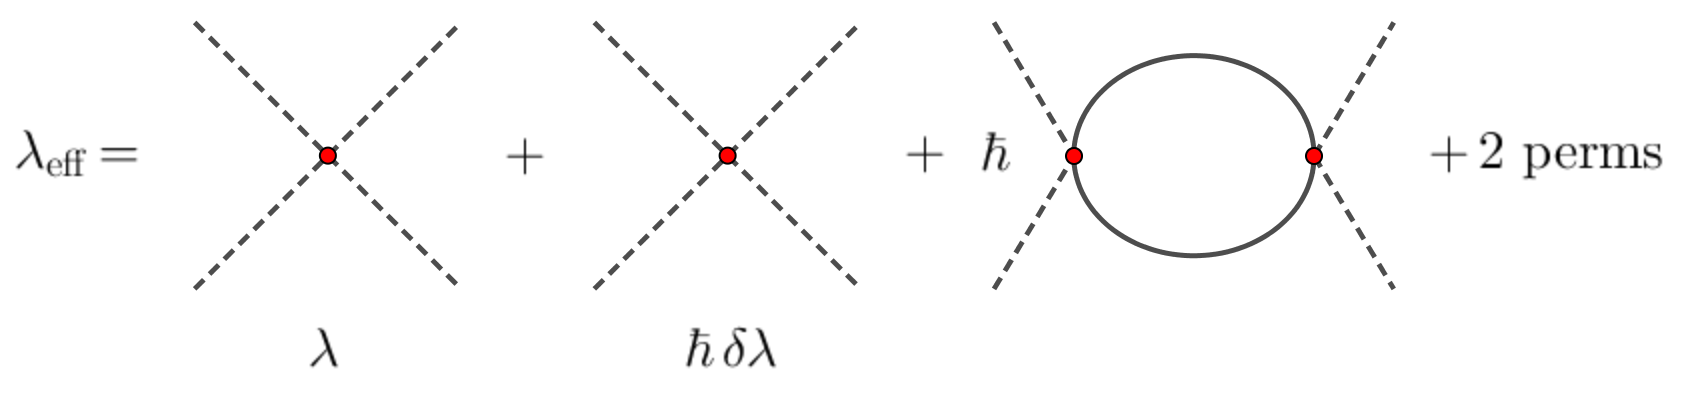
\includegraphics[width=0.9\textwidth]{graphics/aqft/quart1.png}\label{fig:quart1}\end{center}
The loop diagrams in momentum space then have a contribution given by, for example;
\begin{center}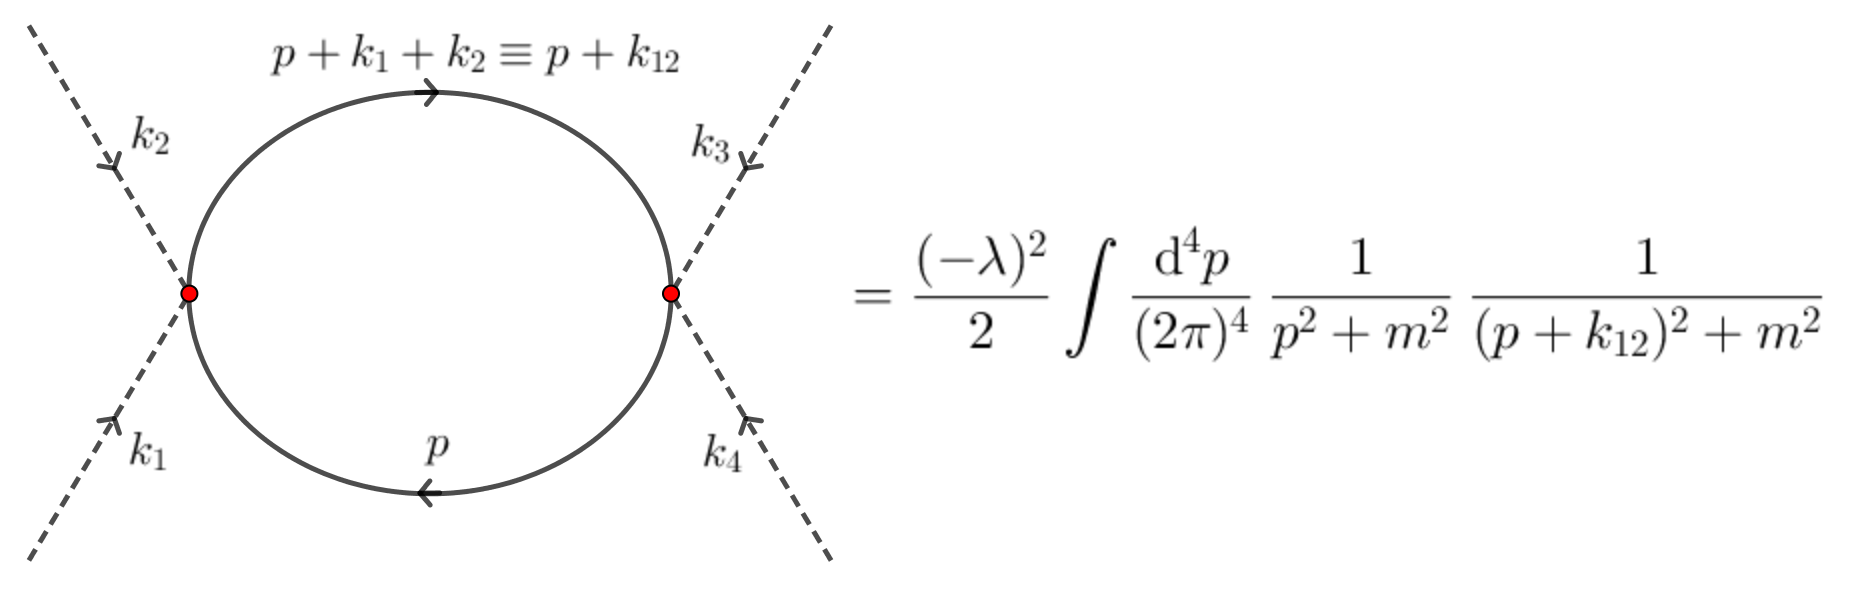
\includegraphics[width=0.7\textwidth]{graphics/aqft/quart2.png}\label{fig:quart2}\end{center}
The fact that these loop integrals depend on the $k_i$ mean that they generate an infinite series of derivative interactions in $\Gamma$ such as $\del_\mu \phi \del^{\mu} \phi \phi^2$. The contribution to the pure $\phi^4$ vertex is independent of the $k_i$ so it is given by;
\begin{equation*}
3 \frac{\lambda^2}{2} \int^{\Lambda_0}{\frac{\ud^4 p}{(2\pi)^4}\frac{1}{(p^2 + m^2)^2}}
\end{equation*}
since each of the three channels contributes equally. This loop integral is logarithmically divergent as $\Lambda_0 \rightarrow \infty$;
\begin{align*}
\frac{3\lambda^2}{2} \int^{\Lambda_0}{\frac{\ud^4 p}{(2\pi)^4}\frac{1}{(p^2 + m^2)^2}} &= \frac{3 \lambda^2}{32 \pi^4}\text{vol}(\mS^{3})\int_0^{\Lambda_0}{\frac{p^3 \ud p}{(p^2 + m^2)^2}} \\
&= \frac{3\lambda^2}{32\pi^4}\text{vol}(\mS^3)\int_0^{\Lambda_0^2 / m^2}{\frac{u \ud u}{(1 + u)^2}} \\
&= \frac{3\lambda^2}{32\pi^2}\left(\log\left(1 + \frac{\Lambda_0^2}{m^2}\right) - \frac{\Lambda_0^2}{\Lambda_0^2 + m^2}\right)
\end{align*}
To get a finite result for $\lambda_{\text{eff.}}$ we tune our initial $\lambda$ using $\delta \lambda$. We might choose;
\begin{equation}
\delta \lambda = \frac{3\lambda^2}{32\pi^2}\left(\log\left(\frac{\Lambda_0^2}{m^2}\right) - 1\right)
\end{equation}
in which case we find that;
\begin{equation}
\lambda_{\text{eff.}} = \lambda - \frac{3\hbar \lambda^2}{32 \pi^2}\left(\log\left(1 + \frac{m^2}{\Lambda_0^2}\right) + \frac{m^2}{m^2 + \Lambda_0^2}\right) + \mO(\hbar^2)
\end{equation}
\subsubsection{The Role of Irrelevant Couplings}
We neglected derivative terms in $\Gamma$ during this calculations. In general though, these are generated and contribute to four particle scattering processes. Using $\Gamma$ we should use all terms with exactly $4$ $\phi$'s. To calculate these we need to actually evaluate the loop integrals at non-zero external momenta. We make use of Feynman's trick;
\begin{equation*}
\frac{1}{AB} = \frac{1}{B - A}\left.\left(\frac{1}{xA + (1 - x)B}\right)\right|_{0}^{1} = \int_0^{1}{\frac{\ud x}{\left(Ax + (1 - x)B\right)^2}}
\end{equation*}
to rewrite;
\begin{align*}
&\frac{1}{(p^2 + m^2)}\frac{1}{\left((p + k_{12})^2 + m^2\right)} \\
& \quad = \int_0^{1}{\frac{\ud x}{\left(x\left((p + k_{12})^2 + m^2\right) + (1 - x)(p^2 + m^2)\right)^2}} \\
& \quad = \int_{0}^{1}{\frac{\ud x}{(p^2 + m^2 + 2x k_{12}\cdot p + xk_{12}^2)^2}} \\
& \quad = \int_{0}^{1}{\frac{\ud x}{\left[(p - xk_{12})^2 + m^2 + x(1 - x)k_{12}\right]^2}}
\end{align*}
So that if $l = p - xk_{12}$ the loop integral becomes;
\begin{equation*}
\frac{\lambda^2}{2}\int_0^{1}{\upd{x}\int{\frac{\ud^4 l}{(2\pi)^4}\frac{1}{\left(l^2 + m^2 + x(1 - x)k_{12}\right)^2}}}
\end{equation*}
We're supposed to integrate this over $\abs{p} \leq \Lambda_0$, however as $\Lambda_0 \rightarrow \infty$ this only differs from the region $\abs{l} \leq \Lambda_0$ by terms of order $k_{12} / \Lambda_0$ which become negligible. In this regime, the loop integral is;
\begin{align*}
&\frac{\lambda^2}{32\pi^4}\text{vol}(\mS^3)\int_0^{1}{\upd{x}\int{\frac{l^3 \ud l}{\left(l^2 + m^2 + x(1 - x)k_{12}^2\right)^2}}} \\
&\quad = \frac{\lambda^2}{32\pi^2}\int_0^{1}{\upd{x}\left(\log\left(\frac{\Lambda_0^2}{m^2 + x(1 - x)k_{12}^{2}}\right) - 1\right)} + \underbrace{\mO\left(\frac{m}{\Lambda_0}, \frac{\abs{k_{12}}}{\Lambda_0}\right)}_{\text{vanishes as }\Lambda_0 \rightarrow \infty}
\end{align*}
Then the total contribution to the $4$-scalar amplitude is;
\begin{align*}
&\mathcal{A}(k_i) = \lambda + \hbar \delta \lambda - \frac{\lambda^2 \hbar}{32 \pi^2}\int_0^{1}{\upd{x}}\left[ \log \frac{\Lambda_0^2}{m^2 + x(1 - x)k_{12}^2} \right.\\
&\qquad \left. + \log \frac{\Lambda_0^2}{m^2 + x(1 - x)k_{23}^2} + \log \frac{\Lambda_0^2}{m^2 + x(1 - x)k_{13}^2} - 3\right]  \\
& \qquad + \mO(\hbar^2, m/\Lambda_0, \abs{k_i}/\Lambda_0)
\end{align*}
Using our earlier choice for $\delta \lambda$ this becomes;
\begin{align*}
&\mathcal{A}(k_i) = \lambda - \frac{\lambda^2 \hbar}{32\pi^2} \int_0^{1}{\upd{x}}\left[ \log\frac{m^2}{m^2 + x(1 - x)k_{12}^2} + \log\frac{m^2}{m^2 + x(1 - x)k_{23}^2}\right. \\
& \qquad \left. + \log\frac{m^2}{m^2 + x(1 - x)k_{13}^2}\right] + \mO(\hbar^2)
\end{align*}
At this order in $\hbar$, we have $\lambda = \lambda_{\text{eff}}$ so that whilst we have generated infinitely many derivative interactions in $\Gamma$, however, they are all finite and completely determined by the values of $(m_p, \lambda_{\text{eff}})$. Now consider starting from a more general classical action at a scale $\Lambda_0$;
\begin{equation*}
S_{\Lambda_0}[\phi] = \int{\upd{^4 x}\frac{1}{2}(\del \phi)^2 + \frac{m^2}{2}\phi^2 + V(\phi)}, \quad V(\phi) = \sum_{k \geq 2}{g_{2k}\Lambda_0^{4 - 2k}\phi^{2k}}
\end{equation*}
At one-loop we now get new contributions to the coefficient of $\phi^{2m}$ in $\Gamma$ coming from the $1$PI e.g. those in \autoref{fig:quart3}. 
\begin{mygraphic}{aqft/quart3}{0.8}{The $1$PI diagrams contributing to the coefficient of $\phi^{2m}$. Each graph has $2m$ external legs in total.}{quart3}\end{mygraphic}
Note that the coefficient of $\phi^{2m}$ is just that coming from the expansion of;
\begin{equation*}
\frac{1}{2}\log \det \left(-\del^2 + m^2 + V^{\prime\prime}(\phi)\right)
\end{equation*}
Now, a loop graph with $e$ propagators contributes an amount proportional to;
\begin{equation*}
\int^{\Lambda_0}{\upd{^4 p }\prod_{j = 1}^{e}{\frac{1}{(p + k_j)^2 + m^2}}}
\end{equation*}
for some $k_j$. As $\Lambda_0 \rightarrow \infty$, this is UV finite unless $e = 1$ ($\Lambda_0^2$ divergent) or $e = 2$ ($\log \Lambda_0$ divergent). Also every time we include a $g_{2k + 2}$ vertex we introduce a power $\Lambda_0^{2 - 2k}$ which a suppression if $k > 1$. In other words, for six or more particles at the vertex. Hence we only get contributions in the continuum limit to $\Gamma$ from graphs built solely from a $\phi^4$ vertex together with a finite correction from the graph with $4$ external legs meeting at a point of a loop $\propto g_6$. We can this latter contribution in our renormalisation scheme.
\subsection{Dimensional Regularisation}\index{dimensional regularisation}
This is qualitatively different to the previous methods of regularisation. It is not a way of regularising the path integral measure, instead we are looking for a way to regularise the asymptotic series that results from the loop integrals. First, make the observation that for any given coupling, it's status as marginal, relevant etc. is dependent on the dimension $d = \dim \mM$. As an example, consider the mass correction at one loop in $\phi^4$ theory. Again we only consider the first diagram in \autoref{fig:phi4two} which contributes;
\begin{equation*}
-\frac{\lambda}{2(2\pi)^4}\int{\frac{\ud^4 p}{p^2 + m^2}} \overset{d \in \mathbb{N}}{\longrightarrow} - \frac{1}{2}\frac{g(\mu) \mu^{4 - d}}{(2\pi)^d} \int{\frac{\ud^d p}{p^2 + m^2}}
\end{equation*}
where we have introduced the dimensionless coupling $g(\mu) = \lambda \mu^{d - 4}$. Now $\mu$ is just some arbitrary scale (e.g. the energy scale of our experiment). Importantly it is \emph{not} a cut off, and so does not take values up to infinity. Then;
\begin{equation*}
-\frac{1}{2}\frac{g(\mu)\mu^{4 - d}}{(2\pi)^{d}}\int{\frac{\ud^d p}{p^2 + m^2}} = -\frac{g(\mu) \mu^{4 - d}}{2(2\pi)^{d}}\text{vol}(\mS^{d - 1})\int_0^{\infty}{\upd{p}\frac{p^{d - 1}}{p^2 + m^2}}
\end{equation*}
To compute the volume (read volume of the manifold not of the $d$-ball), we note that;
\begin{equation*}
\pi^{d/2} = \int_{\RR^{d}}{\prod_{i = 1}^{d}{e^{-x_i^2}}\,\,\ud x_i} = \text{vol}(\mS^{d - 1})\int_0^{\infty}{\upd{r}r^{d - 1}e^{-r^2}} = \text{vol}(\mS^{d - 1})\frac{1}{2}\Gamma\left(\frac{d}{2}\right)
\end{equation*}
So we find that whenever $d \in \mathbb{N}$;
\begin{equation}
\text{vol}(\mS^{d - 1}) = \frac{2\pi^{d/2}}{\Gamma\left(\frac{d}{2}\right)}
\end{equation}
We now define this expression to be $\text{vol}(\mS^{d - 1})$ for $d \in \CC$. The rest of the integral is then;
\begin{align*}
\mu^{4 - d}\int_0^{\infty}{\frac{p^{d - 1}\ud p}{p^2 + m^2}} &= \frac{1}{2}\mu^{d - 4}\int_0^{\infty}{\frac{(p^2)^{(d/2) - 1}\ud (p^2)}{p^2 + m^2}} \\
&= \frac{m^2}{2}\left(\frac{\mu}{m}\right)^{4 - d} \underbrace{\int_0^{1}{(1 - u)^{(d/2) - 1}u^{-d/2}\ud u}}_{\text{beta function}} \\
&= \frac{m^2}{2}\left(\frac{\mu}{m}\right)^{4 - d} \frac{\Gamma(d/2) \Gamma(1 - d/2)}{\Gamma(1)}
\end{align*}
Thus we find that in dimensional regularisation the one loop contribution to $\Pi(k^2)$ is;
\begin{equation*}
\Pi(k^2) = - \frac{g(\mu)m^2}{2(4\pi)^{d/2}}\left(\frac{\mu}{m}\right)^{4 - d} \Gamma(1 - d/2)
\end{equation*}
We should analytically continue this to $d = 4$ by setting $d = 4 - \epsilon$ and using the result;
\begin{equation*}
\Gamma(\epsilon) \sim \frac{1}{\epsilon} - \gamma + \mO(\epsilon)
\end{equation*}
where $\gamma$ is the Euler-Mascheroni constant\index{constant!Euler-Mascheroni}, then we have;
\begin{equation*}
\Pi_{\text{\footnotesize{1-loop}}}(k^2) \sim \frac{g(\mu)m^2}{32\pi^2} \left(\frac{2}{\epsilon} - \gamma + \log\left(\frac{4\pi\mu^2}{m^2}\right)\right) + \mO(\epsilon)
\end{equation*}
The divergence in the $1$-loop $\Pi(k^2)$ as $\Lambda_0 \rightarrow \infty$ has become the pole $1/\epsilon$. In particular note that the logarithm is perfectly finite since $\mu$ is not a cut off.
\subsubsection{The $\bar{\text{\textbf{MS}}}$ Renormalisation Scheme}
We fix the counterterm $\delta m^2$ by requiring a finite result in $d = 4$ so we have to remove the $1/\epsilon$ term. Just doing this is minimal substitution (MS). Often it is convenient to also remove the $\gamma$ and $4\pi$ terms. This is modified minimal subtraction. So we choose;
\begin{equation*}
\delta m^2 = - \frac{g(\mu)m^2}{32\pi^2}\left(\frac{2}{\epsilon} - \gamma + \log 4\pi\right)
\end{equation*}
in the $\bar{\text{MS}}$ scheme. Thus we have;
\begin{equation*}
\Pi(k^2) = \frac{g(\mu)m^2}{32\pi^2}\log\left(\frac{\mu^2}{m^2}\right)
\end{equation*}
which is now finite as $d \rightarrow 4$. For the $\phi^4$ term, the loop corrections come from the same integrals computed above in the renormalisation of the quartic coupling;
\begin{equation*}
\frac{g^{2}(\mu)\mu^{4 - d}}{2}\int{\frac{\ud^{d}p}{(2\pi)^{d}}\frac{1}{p^2 + m^2}\frac{1}{(p + k_{12})^2 + m^2}}
\end{equation*}
along with other channels. Again if we are just interested in the pure quartic coupling then we can set $k_{ij} = 0$ and find the contribution;
\begin{align*}
\frac{3g^{2}(\mu)\mu^{4 - d}}{32\pi^4}\text{vol}(\mS^{d - 1})\int_0^{\infty}{\frac{p^{d - 1}\ud p}{(p^2 + m^2)^2}} &= \frac{3g^2}{2(4 \pi)^{d/2}}\left(\frac{\mu}{m}\right)^{4 - d}\Gamma(2 - d/2) \\
&\sim \frac{3g^2}{32\pi^2}\left(\frac{2}{\epsilon} - \gamma + \log\frac{4\pi \mu^2}{m^2}\right) + \mO(\epsilon) 
\end{align*}
Then we choose out counterterm to remove this pole;
\begin{equation}
\delta g = \frac{3g^2}{32\pi^2}\left(\frac{2}{\epsilon} - \gamma + \log 4\pi\right)
\end{equation}
again in the $\bar{\text{MS}}$ scheme. So we find a $\phi^{4}$ coupling in the $1$PI effective action of;
\begin{equation*}
g_{\text{eff}}(\mu) = g(\mu) - \frac{3\hbar g^{2}(\mu)}{32\pi^2}\log\left(\frac{\mu^2}{m^2}\right) + \mO(\hbar^2)
\end{equation*}
The scale $\mu$ was merely a choice of units and we are now in exactly $d = 4$ so $g_{\text{eff}}$ can't depend on $\mu$. This is compatible with our result if;
\begin{align*}
\mu\frac{\del g_{\text{eff}}}{\del \mu} &= 0 = \mu\frac{\del}{\del \mu}\left(g(\mu) - \frac{3\hbar g^2(\mu)}{16\pi^2}\log\left(\frac{\mu}{m}\right) + \mO(\hbar^2)\right) \\
\Rightarrow \beta(g) &= \mu \frac{\del g}{\del \mu} = \frac{3\hbar g^2}{16\pi^2} + \mO(\hbar^2)
\end{align*}
i.e. $g(\mu)$ is marginally irrelevant. Solving this for the coupling we see that;
\begin{equation}
\frac{1}{g(\mu\pr)} = \frac{1}{g(\mu)} + \frac{3\hbar}{16\pi^2}\log\left(\frac{\mu}{\mu\pr}\right) + \mO(\hbar^2)
\end{equation}
Now, if we just solved the original path integral exactly, we would find of course that $\Gamma(\phi)$ is independent of $\mu$. But since we are working perturbatively, it is ambiguous as to whether we should do perturbation theory in $g(\mu)$ or $g(\mu\pr)$. In fact we actually have no choice; there is a scale inherent in $\phi^4$ theory, $\mu\pr = \Lambda_{\phi^4}$ where $g(\mu\pr)^{-1} = 0$. In other words we find;
\begin{equation*}
g(\mu) = \frac{16\pi^2}{3\hbar}\frac{1}{\log(\Lambda_{\phi^4}/\mu)}
\end{equation*}
\subsection{One-loop Renormalisation of QED}\index{QED}
We start with the action;
\begin{equation}
S_{\text{QED}} = \int{\upd{^4 x}\frac{1}{4e^2}F_{\mu\nu}F^{\mu\nu} + \bar{\psi}(\slashed{D} + m)\psi}
\end{equation}
where $D_\mu = \del_\mu + i A_\mu$ and $(\gamma^{\mu})\dagg = - \gamma^{\mu}$ in the Euclidean signature. THis means that the $\text{SO}(4)$ generators $S^{\mu\nu} = \tfrac{1}{4}[\gamma^{\mu}, \gamma^{\nu}]$ are all hermitian and $\bar{\psi} = \psi\dagg$. We rescale the photon field; $A^{\text{new}} = A^{\text{old}}/e$ so that;
\begin{equation*}
S_{\text{QED}}[A^{\text{new}}, \psi] = \int{\upd{^4 x}\frac{1}{4}F^2 + \bar{\psi}(\slashed{\del} + m)\psi + ie\bar{\psi}\slashed{A}\psi}
\end{equation*}
In momentum space, the Maxwell term becomes;
\begin{equation*}
\frac{1}{4}\int{\upd{^4 x}F_{\mu\nu}F^{\mu\nu}} = \frac{1}{2}\int{\upd{^4 k}k^2 \left(\delta^{\mu\nu} - \frac{k^{\mu}k^{\nu}}{k^2}\right)A_{\mu}(-k)A_{\nu}(k)}
\end{equation*}
from which we can read off the free photon propagator;
\begin{equation*}
\Delta^{(0)}_{\mu\nu}(k) = \frac{1}{k^2}\left(\delta^{\mu\nu} - \frac{k^{\mu}k^{\nu}}{k^2}\right)
\end{equation*}
In the Lorenz gauge\index{gauge!Lorenz}, $\del^{\mu}A_\mu = 0$ which gives the gauge condition $k^{\mu}\Delta^{(0)}_{\mu\nu}(k) = 0$. This implies that only transverse polarisations propagate.
\subsubsection{Vacuum Polarisation}\index{polarisation!vacuum}
In the quantum theory, the exact photon propagator receives corrections as the photon interacts with the electron;
\begin{align*}
\Delta_{\mu\nu}(k) &= \int{\upd{^4 x}e^{ik\cdot x}\left< A_{\mu}(x)A_{\nu}(0) \right>} \\
&= \Delta_{\mu\nu}^{(0)}(k) + \Delta^{(0)}_{\mu \rho}(k)\Pi^{\rho\sigma}(k)\Delta^{(0)}_{\sigma \nu}(k) + \cdots
\end{align*}
where $\Pi_{\rho \sigma}(k)$ is the sum of all $1$PI diagrams with $2$ external photons. This takes the form;
\begin{equation*}
\Pi_{\rho \sigma} = k^2\left(\delta_{\rho \sigma} - \frac{k_\rho k_\sigma}{k^2}\right)\pi(k^2)
\end{equation*}
for some function $\pi(k^2)$. Then the factor in brackets is a projection operator $P\indices{^{\rho}_{\sigma}}$ satisfying $P\indices{^{\rho}_{\kappa}}P\indices{^{\kappa}_{\sigma}} = P\indices{^{\rho}_{\sigma}}$. Then we see that;
\begin{equation*}
\Delta_{\mu\nu}(k) = \Delta_{\mu\nu}^{(0)}(k)\left(1 + \pi(k^2) + \pi^2(k^2) + \cdots\right). = \frac{\Delta_{\mu\nu}^{(0)}(k)}{1 - \pi(k^2)}
\end{equation*}
Just as in the scalar case where the classical propagator was the inverse of the kinetic term in the effective action, here we have;
\begin{equation*}
\Gamma_{\text{eff}}[A] = \frac{1}{2}\int{\upd{^4 k} \left(1 - \pi(k^2)\right)A_\mu(-k)k^2 \left(\delta^{\mu\nu} - \frac{k^{\mu}k^{\nu}}{k^2}\right)A_\nu(k)}
\end{equation*}
In particular expanding $\pi(k^2) = \pi(0) + \cdots$ the leading piece gives;
\begin{equation*}
\Gamma_{\text{eff}}^{(2)}[A] = \int{\upd{^4 x}\frac{1 - \pi(0)}{4}F_{\mu\nu}F^{\mu\nu}}
\end{equation*}
Which governs the leading order wavefunction renormalisation.\index{renormalisation!wavefunction} We compute this via dimensional regularisation, and introduce a dimensionless coupling $g^2(\mu) = e^2 \mu^{d - 4}$ for some experimental scale $\mu$. The vertex is then;
\begin{equation*}
ig(\mu)\mu^{(4 - d)/2}\int{\upd{^d x}\bar{\psi}\slashed{A}\psi}
\end{equation*} 
The leading order correction is then governed by the diagram;
\begin{mygraphic}{aqft/vacpol}{0.8}{The leading order correction to the photon propagator.}{vacpol}\end{mygraphic}
Before writing down the correction, we should understand that a loop in a fermion diagram introduces an overall minus sign. This is really a statement of Wick's theorem and the fact that the components of $\psi$ are Grassman variables. Expanding $\exp\left(- S_{\text{QED}}[A, \psi]/\hbar\right)$ in powers of the vertex we have contributions of the form;
\begin{equation*}
\left< \bar{\psi} \gamma^{\mu}\psi(x_1) \bar{\psi} \cdots \psi(x) \bar{\psi}\gamma^{\rho}\psi(x_n) \right>
\end{equation*}
Joining up $\psi \bar{\psi}$ contributions we find that the first and last are in the opposite order. To get a propagator we need to bring the $\psi$ past the $\bar{\psi}$ which introduces an extra minus sign. Then we find;
\begin{align*}
\Pi^{\rho \sigma}_{\text{1-loop}}(k) &= -(-ig)^2 \mu^{4 - d}\int{\frac{\ud^d p}{(2\pi)^d}\tr\left(\frac{1}{i\slashed{p} + m}\gamma^{\rho}\frac{1}{i(\slashed{p} - \slashed{k}) + m}\gamma^{\sigma}\right)} \\
&= \frac{g^2(\mu)\mu^{4 - d}}{(2\pi)^d}\int{\upd{^d p}\frac{\tr \left((-i \slashed{p} + m)\gamma^{\rho}(-i \slashed{p} - i\slashed{k} + m)\gamma^{\sigma}\right)}{(p^2 + m^2)\left((p - k)^2 + m^2\right)}}
\end{align*}
This integral can be done (apparently) and we find;
\begin{equation}
\Pi_{\text{1-loop}}^{\rho\sigma}(k^2) = (k^2 \delta^{\rho\sigma} - k^{\rho}k^{\sigma})\pi_{\text{1-loop}}(k^2)
\end{equation}
where;
\begin{equation}
\pi_{\text{1-loop}}(k^2) = \frac{-8 g^{2}(\mu)\Gamma(2 - d/2)}{(4\pi)^{d/2}}\int_0^{1}{\upd{x} x(1 - x)\left(\frac{\mu^2}{\Delta}\right)^{2 - d/2}}
\end{equation}
where $\Delta = m^2 + k^2 x(1 - x)$. This expression diverges in $d = 4$ as we would expect, so we need to tune using a couterterm;
\begin{equation*}
\int{\frac{\delta Z_3}{4}F_{\mu\nu}F^{\mu\nu}}
\end{equation*}
Writing $d = 4 - \epsilon$ we have;
\begin{equation*}
\pi_{\text{1-loop}}(k^2) \sim -\frac{g^2(\mu)}{2\pi^2}\int_0^{1}{\upd{x}x(1 - x)\left(\frac{2}{\epsilon} - \gamma + \log \frac{4\pi \mu^2}{\Delta} + \mO(\epsilon)\right)}
\end{equation*}
In the $\bar{\text{MS}}$ scheme then, we take $\delta Z_3$ to absorb the divergent parts of the above;
\begin{equation}
\delta Z_3 = -\frac{g^2(\mu)}{12\pi^2}\left(\frac{2}{\epsilon} - \gamma + \log 4\pi\right)
\end{equation}
So we find that $\Pi^{\rho\sigma}(k^2) = k^2 P^{\rho\sigma}\pi(k^2)$ with;
\begin{equation}
\pi(k^2) = \frac{g^2}{2\pi^2}\int{\upd{x}x(1 - x)\log\left(\frac{m^2 + x(1 - x)k^2}{\mu^2}\right)} + \mO(\hbar, \epsilon)
\end{equation}
\subsubsection{The $\beta$-function of QED}
We have;
\begin{align*}
\Gamma_{\text{eff}}[A^{\text{old}}] &= \frac{1}{4g_{\text{eff}}^2}\int{\upd{^4 x}F_{\mu\nu}F^{\mu\nu}} + \cdots \\
&= \frac{1 - \pi(0)}{4g^2(\mu)}\int{\upd{^4 x} F^2 + \cdots} \\
&= \frac{1}{4}\left(\frac{1}{g^2(\mu)} - \frac{\hbar}{12\pi^2}\log\left(\frac{m^2}{\mu^2}\right) + \mO(\hbar^2)\right)\int{\upd{^4 x}F^2}
\end{align*}
So our vacuum polarisation result also tells us the $\beta$-function of QED. Since the physically measured coupling $g_{\text{eff}}(\mu)$ cannot depend on $\mu$ we have;
\begin{equation*}
0 = \mu\frac{\del}{\del \mu}\left(\frac{1}{g^2} - \frac{\hbar}{12\pi^2} \log\frac{m^2}{\mu^2} + \mO(\hbar^2)\right)
\end{equation*}
So we find that;
\begin{align*}
-\frac{2}{g^3(\mu)}\beta(g) + \frac{\hbar}{6\pi^2} + \mO(\hbar^2) &= 0 \Rightarrow \beta(g) = \frac{\hbar g^3}{12\pi^2} + \mO(\hbar^2)
\end{align*}
Thus we find that;
\begin{equation}
\frac{1}{g^{\prime 2}(\mu\pr)} = \frac{1}{g^2(\mu)} + \frac{\hbar}{6\pi^2}\log\left(\frac{\mu}{\mu\pr}\right)
\end{equation}
From experiment we know that at $\mu \sim m_e \sim 511 \,\,\text{keV}$, we have $\alpha \sim 1/137$, which gives;
\begin{equation*}
g^2(\mu) = \frac{6\pi^2}{\hbar} (\log\frac{\Lambda_{\text{QED}}}{\mu})^{-1}
\end{equation*}
where $\Lambda_{\text{QED}} \sim 10^{236}\,\,\text{GeV}$. So again as in the case of $\phi^4$, there is no continuum theory of QED, it is only valid up to the scale determined by $\Lambda_{\text{QED}}$. This is of no practical consequence as QED ultimately merges with the weak force at an energy scale far below $\Lambda_{\text{QED}}$.
\newpage
\section{Symmetries in QFT}
Suppose we have a change of variables $\phi^a \mapsto \phi^{\prime a} = \phi^a + \epsilon^{r}f^{a}_r(\phi, \del_\mu \phi)$, such that the Lagrangian transforms as $\mL \mapsto \mL + \del^\mu(K_{\mu r} \epsilon^r)$, then the equations of motion will be unaffected and we say that the transformation is symmetry of the classical theory. Noether's theorem further tells us that the current;
\begin{equation*}
J_{\mu r} = \frac{\delta \mL}{\delta(\del^\mu \phi^a)}f_r^a(\phi, \del_\mu \phi) - K_{\mu r}
\end{equation*}
is conserved if the equations of motion hold. We need to re-examine this in the quantum theory. We have two options;
\begin{itemize}
\item Look at general correlation functions
\item Look at the quantum effective action\index{action!quantum effective}
\end{itemize}
We will begin with the second point of view.
\subsection{Symmetries of the Effective Action}
Formally, under $\phi^a \mapsto \phi^{\prime a}$ we would expect $\mD \phi \mapsto \mD \phi\pr$ where;
\begin{equation*}
\mD \phi\pr = \mD \phi \det\left(\frac{\delta \phi^{\prime a}(x)}{\delta \phi^b(y)}\right)
\end{equation*} 
where;
\begin{equation*}
\frac{\delta \phi^{\prime a}(x)}{\delta \phi^b(y)} = \delta\indices{^{a}_{b}}\delta(x - y) + \epsilon^{r}\frac{\delta f_r^a(\phi, \del \phi)}{\delta \phi^b(y)} + \mO(\epsilon^2)
\end{equation*}
So we find that;
\begin{equation*}
\det\left(\frac{\delta \phi^{\prime a}(x)}{\delta \phi^b(y)}\right) = 1 + \tr \epsilon^r \frac{\delta f_r^a(\phi, \del \phi)}{\delta \phi^b(y)} + \mO(\epsilon^2)
\end{equation*}
which is a trace over the flavour indices $a, b$ as well as a functional trace over $x, y$. We'll be interested in transformations for which $\mD \phi = \mD \phi\pr$. In this case consider the partition function;
\begin{equation*}
\mZ[\vec{J}] = \int{\mD \phi\pr \,\,\exp\left(-\frac{1}{\hbar}\left(S[\phi] + \int{\upd{^d x}J_a(x)\phi^{\prime a}(x)}\right)\right)}
\end{equation*}
Using the fact that we have a symmetry;
\begin{align*}
\mZ[\vec{J}] &= \int{\mD \phi \,\,\exp\left(-\frac{1}{\hbar}\left(S[\phi] + \int{\upd{^d x}J_a(x)\phi^a(x)} + \int{\upd{^d x}J_a \epsilon^r f^a_r}\right)\right)} \\
&= \int{\mD \phi \,\, \exp\left(- \frac{1}{\hbar}\left(S[\phi] + \int{\upd{^d x}J\phi}\right)\right)} \\ 
&\qquad \qquad \qquad \qquad \times \left\{1 - \frac{\epsilon^r}{\hbar}\int{\upd{^d x}J_a f_r^a(\phi, \del \phi)} + \mO(\epsilon^2)\right\} \\
&= \mZ[\vec{J}] - \frac{\epsilon^r}{\hbar}\mZ[\vec{J}] \left< \int{\upd{^d x}J_a f^a_r(\phi, \del\phi)} \right>_{\vec{J}} + \mO(\epsilon^2)
\end{align*}
So we see that this implies;
\begin{equation}
\int{\upd{^d x}J_a(x)\left< f^a_r(\phi, \del \phi) \right>_{\vec{J}}} = 0
\end{equation}
We want to write this in terms of the quantum effective action, $\Gamma[\Phi]$. Recall that $\Gamma[\Phi]$ is the Legendre transform of $W[\vec{J}]$ where $\vec{J}$ is evaluated at the extremum;
\begin{equation*}
J_\phi^a = -\frac{\delta \Gamma[\Phi]}{\delta \Phi^a}
\end{equation*}
such that $\left< \phi^a \right>_{\vec{J}_\phi} = \Phi^a$, where $\Phi^a$ is the field in the $1$PI effective action. At this value, our condition becomes;
\begin{equation*}
\int{\upd{^d x}\frac{\delta \Gamma[\Phi]}{\delta \Phi^a} \left< f_r^a(\phi, \del \phi) \right>_{\vec{J}_\phi}} = 0
\end{equation*}
In other words, the quantum effective action is invariant under;
\begin{equation*}
\Phi^a \mapsto \Phi^{\prime a} = \Phi^a + \epsilon^r \left< f^a_r(\phi, \del \phi) \right>_{\vec{J}_\phi}
\end{equation*}
As a special case (and an important one), suppose that $f$ is actually linear in $\phi$ i.e.
\begin{equation*}
f^a_r(\phi, \del\phi) = c_r^a(x) + \int{\upd{^d x}d_{rb}(x, y)\phi^b(y)}
\end{equation*}
Then we have the following (note that this \emph{only} holds in the case that $f$ is linear);
\begin{equation}
\left< f^a_r(\phi, \del \phi) \right>_{\vec{J}_\phi} = f_r^a\left(\left< \phi \right>_{\vec{J}_\phi}, \left< \del \phi \right>_{\vec{J}_\phi}\right) = f_r^a(\Phi, \del \Phi)
\end{equation}
Thus, in this case, $\Gamma[\Phi]$ is invariant under $\Phi^a \mapsto \Phi^a + \epsilon^r f_r^a(\Phi, \del \Phi)$, and so has th same symmetry as the classical action, $S[\phi]$. So if we can find a classical action with a symmetry at linear order under which the path integral measure is invariant, then it will be a symmetry of the full quantum theory. As an example consider;
\begin{equation*}
S[\phi] = \int{\upd{^d x}\frac{1}{2}(\del\phi)^2 + \frac{1}{2}m^2 \phi^2 + \lambda \phi^4}
\end{equation*}
then $S[\phi] = S[-\phi]$. Now, \emph{provided we regularise} in a way that is compatible with this $\ZZ_2$ symmetry, we will also have $\Gamma[\Phi] = \Gamma[-\Phi]$ i.e. we can't generate terms like $\Phi^3, \Phi^7$ etc. As another example suppose we have the action;
\begin{equation*}
S[\phi^a] = \int{\upd{^d x}\frac{1}{2}\delta_{ab}\del \phi^a \del \phi^b + \frac{m^2}{2}\delta_{ab}\phi^a \phi^b + \frac{\lambda}{4}(\phi^a \phi^b \delta_{ab})^2}
\end{equation*}
then this is invariant under $\text{SO}(n)$ rotations $\phi^a \rightarrow \phi^a + \omega\indices{^{a}_{b}}\phi^b$ so that;
\begin{equation*}
\frac{\delta f^a(\phi, \del \phi)}{\delta \phi^b(y)} = \omega\indices{^{a}_{b}}\delta(x - y)
\end{equation*}
which is field independent. So provided we treat all components of the field the same when we regularise, the effective action will also be $\text{SO}(n)$ invariant.

\paraskip
As a final example, suppose we have an $\text{SO}(d)$ transformation of the co-ordinate system $x^{\mu}\mapsto L\indices{^{\mu}_{\nu}}x^{\nu}$ with $L \in \text{SO}(d)$. This induces a transformation on the fields;
\begin{equation*}
A_\mu(x) \mapsto (L^{-1})\indices{_{\mu}^{\nu}}A_\nu(L^{-1}x) , \quad \psi^\alpha \mapsto S\indices{^{\alpha}_{\beta}}(L)\psi^\beta(L^{-1}x)
\end{equation*}
where $S\indices{^{\alpha}_{\beta}}(L) = \exp(\tfrac{i}{4}L_{\mu\nu}[\gamma^\mu, \gamma^\nu])\indices{^{\alpha}_{\beta}}$ are the $\text{SO}(d)$ generators in the Dirac spinor representation. Then, $S_{\text{QED}}[A, \psi]$ is $\text{SO}(d)$ invariant, and so to will $\Gamma_{\text{QED}}[A, \psi]$ provided we regularise in an $\text{SO}(d)$ invariant way.\footnote{This might be by imposing a cut off on the eigenvalues of $-\Box$, or working with $d \in \CC$, but it will \emph{not} be by working on a lattice $\Lambda \subset \RR^{d}$, which will not respect the full $\text{SO}$(d) invariance.} In general, there are three possibilities;
\begin{enumerate}
\item There exists a symmetry compatible regularisation which we go ahead and use. Then the regularised quantum theory will also have this symmetry manifest at every stage.
\item There exists a symmetry compatible regularisation which we do not use. In this case the regularised theory and counterterms will not respect the symmetry. However, the symmetry will be restored in the continuum limit.
\item There does not exist any symmetry compatible regularisation. The symmetry is then absent in the quantum theory despite being present at the classical level, and is said to be an \emph{anomaly}\index{anomaly}. 
\end{enumerate}
As an explicit example of this last point, consider;
\begin{equation*}
S[\phi] = \int{\upd{^4 x}\frac{1}{2}(\del \phi)^2 + \frac{\lambda}{4!}\phi^4}
\end{equation*}
This is invariant under conformal transformations\index{conformal transformation}, $\delta \mapsto e^{2\sigma}\delta$, $\phi \mapsto e^{-\sigma}\phi$ where $\sigma \in \RR$. Since $\mC = \set{\phi : \RR^4 \rightarrow \RR}$ is a vector space, we could give it a metric;
\begin{equation*}
\ud s^2_{\mC} = \int_{\RR^4}{\upd{^4 x}\abs{\delta \phi}^2}
\end{equation*}
and take the path integral measure to be the Riemannian measure associated to this metric. But this measure is \emph{not} conformally invariant. We thus do not expect our quantum theory to be conformal, and indeed this is confirmed in the beta functions.
\subsection{Ward-Takahashi Identities}\index{Ward-Takahashi identity}
Symmetries also place constraints on the correlation functions. Suppose $\mO_i(\phi)$ vary under a symmetry transformation $\phi \mapsto \phi\pr$ as $\mO_i(\phi) \mapsto \mO_i(\phi\pr)$ (i.e. they have no spin indices etc.), then;
\begin{equation*}
\int{\mD \phi\pr\,\,e^{-S[\phi\pr]/\hbar}\mO_1\left(\phi\pr(x_1)\right)\cdots\mO_n\left(\phi\pr(x_n)\right)} = \int{\mD \phi\,\,e^{-S[\phi]/\hbar}\prod_{i = 1}^{n}{\mO_i\left(\phi\pr(x_i)\right)}}
\end{equation*}
So we see that this implies;
\begin{equation}
\left< \mO_1\left(\phi(x_1)\right)\cdots\mO_n\left(\phi(x_n)\right) \right> = \left< \mO_1\left(\phi\pr(x_1)\right) \cdots \mO_n\left(\phi\pr(x_n)\right)\right>
\end{equation}
This is the (global) Ward-Takahashi identity. As an example consider the action for a complex scalar field;
\begin{equation*}
S[\phi] = \int{\upd{^d x}\frac{1}{2}\del^{\mu} \bar{\phi}\del_\mu\phi + V\left(\abs{\phi}^2\right)}
\end{equation*}
Then this is invariant under $\phi \mapsto e^{i\alpha}\phi$ and $\bar{\phi} \mapsto e^{-i\alpha}\bar{\phi}$, $\alpha \in \RR$. Then suppose we insert operators of the form $\mO_i(x) = \phi^{r_i}(x)\bar{\phi}^{s_i}(x)$. The Ward-Takahashi identity gives;
\begin{equation*}
\left< \prod_{i = 1}^{n}{\mO_i(x_i)} \right> = \exp\left(i\alpha \sum_{i = 1}^{n}(r_i - s_i)\right)\left< \prod_{i = 1}^{n}{\mO_i(x_i)} \right>
\end{equation*}
and so we deduce that the correlator vanishes unless $\sum{r_i} = \sum{s_i}$ since the above holds for all $\alpha \in \RR$. This is known as a \emph{selection rule}\index{selection rule}.

\paraskip
Similarly, consider spacetime translations $x \mapsto x\pr = x - a$ where $a \in \RR^{d}$. Then $\phi\pr(x) = \phi(x - a)$ for a scalar field. If this is a symmetry then inserting operators that only depend on $x$ through their dependence on the fields implies that;
\begin{equation*}
\left< \prod_{i = 1}^{n}{\mO_i(x_i)} \right> = \left< \prod_{i = 1}^{n}{\mO_{i}(x_i - a)} \right>
\end{equation*}
which allows us to deduce that the correlator can only be a function of the differences $\left(x_i - x_j\right)$. Suppose further that our theory was $\text{SO}(d)$ invariant, then the correlators of scalar operators could only depend on the $\text{SO}(d)$ invariant separations $(x_i - x_j)^2$.
\subsection{Current Conservation in QFT}
Suppose that our transformation $\phi^a \mapsto \phi^a + \epsilon^r f_r^a(\phi, \del \phi)$ leaves the Lagrangian, $\mL(\phi)$, invariant not just the action, and also preserves the path integral measure $\mD \phi$. Then we have a local conservation law for constant $\epsilon$. Just as in Noether's theorem, if we allow $\epsilon^r \mapsto \epsilon^r(x)$, the action can only vary by terms $\del_\mu \epsilon^r(x)$. So our partition function becomes;
\begin{equation*}
\mZ = \int{\mD \phi\pr \,\, e^{-S[\phi\pr]/\hbar}} = \int{\mD \phi e^{-S[\phi]/\hbar}\left(1 - \int_{\mM}{\upd{^d x}j^\mu(x)\del_\mu \epsilon^r(x)} + \mO(\epsilon^2)\right)}
\end{equation*}
where now $j^{\mu}(x)$ may contain contributions from the path integral measure as well as just the field transformation. To first order in $\epsilon^r$ we see that this is simply;
\begin{equation*}
\int_{\mM}{\upd{^d x}\left< j^{\mu}_r(x) \right>\del_\mu \epsilon^r(x)} = 0
\end{equation*}
Integrating by parts, this simply says that the expectation of $\left< j^{\mu}_r(x) \right>$ is conserved;\footnote{With the standard set of assumptions that $\mM$ is compact/there are no boundary terms etc.}
\begin{equation}
\del_\mu \left< j^{\mu}_r(x) \right> = 0
\end{equation}
In the presence of operators, this doesn't hold as is, instead the operators themselves change infinitesimally under the transformation $\phi \mapsto \phi\pr$, 
\begin{equation*}
\mO_i \mapsto \mO_i + \epsilon^r (\delta_r \mO_i)
\end{equation*}
Then carrying out a similar procedure to the one above we find;
\begin{multline*}
\int{\mD\phi\pr\,\,e^{-S[\phi\pr]/\hbar}\prod_{i = 1}^{n}{\mO\pr_i(x_i)}} \\ = \int{\mD \phi\,\,e^{-S[\phi]/\hbar}\left(1 - \int_{\mM}{\upd{^d x}j^\mu_r(x)\del_\mu \epsilon^r(x)} + \mO(\epsilon)\right)} \\ \times \left(\prod_{i = 1}^{n}{\mO_i(x_i)} + \sum_{i = 1}^{n}\epsilon^r(x_i)(\delta_r\mO_i)\prod_{j \neq i}{\mO_j(x_j)}\right)
\end{multline*}
After performing a completely analogous integration by parts and equating the first term with the left hand side, we see that;
\begin{align*}
\int_{\mM}{\upd{^d x}\epsilon^r(x)\del_\mu\left< j_r^{\mu}(x)\prod_{i = 1}^{n}{\mO_i(x_i)} \right>} &= -\sum_{i = 1}^{n}{\epsilon^r(x_i)\left< \left(\delta_r \mO_i(x_i)\right)\prod_{j \neq i}{\mO_j(x_j)} \right>} \\
&\hspace{-100pt}= -\sum_{i = 1}^{n}\int{\upd{^d x}\delta^{(d)}(x - x_i)\epsilon^r(x)\left< \delta_r \mO_i(x_i)\prod_{j \neq i}{\mO_j(x_j)} \right>}
\end{align*}
Thus we find the local form of the Ward-Takahashi identity;
\begin{equation}
\del_\mu\left< j^\mu_r(x)\prod_{i = 1}^{n}{\mO_i(x_i)} \right> = -\sum_{i = 1}^{n}{\delta^{(d)}(x - x_i)\left< \delta_r\mO_i(x_i)\prod_{j \neq i}{\mO_j(x_j)} \right>}
\end{equation}
This generalises current conservation in the classical theory and says that the correlator is conserved except at the operator insertion points, integrating over all of $\mM$ we find;
\begin{equation*}
0 = \sum_{i = 1}^{n}{\left< \delta_r(x_i)\prod_{j \neq i}{\mO(x_j)} \right>} = \delta_r\left< \prod_{i = 1}^{n}{\mO_i(x_i)} \right>
\end{equation*}
which reproduces the global identity for $\phi \mapsto \phi + \delta \phi$.
\subsection{Ward-Takahashi Identity in QED}
The QED action;
\begin{equation*}
S[A, \psi] = \int{\upd{^d x}\frac{1}{4e^2}F_{\mu\nu}F^{\mu\nu} + \bar{\psi}(\slashed{D} + m)\psi}
\end{equation*}
is invariant under the global transformation $\psi \mapsto e^{i\alpha}\psi$, $\bar{\psi} \mapsto e^{-i\alpha}\bar{\psi}$, $A_\mu \mapsto A_\mu$ (so this is not a gauge transformation), where $\alpha \in \RR$. As in our earlier discussion, this is a symmetry of the quantum theory providing our regularised path integral measure integrates over as many $\psi$ modes as $\bar{\psi}$ modes. Now, promoting $\alpha \rightarrow \alpha(x)$ we generate a Noether current $j^{\mu} = i \bar{\psi}\gamma^{\mu}\psi$, assuming that the path integral measure stays invariant. For infinitesimal $\alpha$ we have;
\begin{equation*}
\delta \psi = i \alpha \psi, \qquad \delta \bar{\psi} = -i \alpha \bar{\psi}
\end{equation*}
so that the local Ward-Takahashi identity for $\left< \psi(x_1)\bar{\psi}(x_2) \right>$ is;
\begin{multline*}
\del_\mu\left< j^{\mu}(x)\psi(x_1)\bar{\psi}(x_2) \right> \\ = -i\delta^{(4)}(x - x_1)\left< \psi(x_1)\bar{\psi}(x_2) \right> + \delta^{(4)}(x - x_2)\left< \psi(x_1)\bar{\psi}(x_2) \right>
\end{multline*}
In momentum space we see that;
\begin{align*}
&\int{\ud^4 x_1\upd{^4 x_2}e^{ik_1 \cdot x_1}e^{-ik_2\cdot x_2}\left< \psi(x_1)\bar{\psi}(x_2) \right>} \\
&\hspace{50pt}= \int{\ud^4 x_1 \upd{^4 x_2} e^{ik_1\cdot x_1}e^{-ik_2\cdot x_2}\left< \psi(x_1 - x_2)\bar{\psi}(0) \right>} \\
&\hspace{50pt}= (2\pi)^4 \delta^{(4)}(k_1 - k_2)S(k_1)
\end{align*}
where $S(k)$ is the exact electron propagator, so as before we have;
\begin{align*}
S(k) &= \frac{1}{i\slashed{k} + m} + \frac{1}{i\slashed{k} + m}\Sigma(\slashed{k}) \frac{1}{i\slashed{k} + m} + \cdots \\
&= \frac{1}{i\slashed{k} + m - \Sigma(\slashed{k})}
\end{align*}
where $\Sigma(\slashed{k})$ is the electron self-energy. We can also define the exact electromagnetic vertex $\Gamma_\mu(k_1, k_2)$ as follows;
\begin{align*}
&\int{\ud^4 x\ud^4 x_1 \upd{^4 x_2}e^{ip\cdot x}e^{ik_1\cdot x_1}e^{-ik_2\cdot x_2}\left< j_\mu(x)\psi(x_1)\bar{\psi}(x_2) \right>} \\
&\qquad= \int{\ud^4 x\ud^4 x_1 \upd{^4 x_2}e^{ip\cdot(x - x_2)}e^{ik_1\cdot(x_1 - x_2)}e^{-i(p + k_1 - k_2)\cdot x_2}} \\
&\qquad \qquad \times \left< j_\mu(x - x_2) \psi(x_1 - x_2) \bar{\psi}(0)\right> \\
&\qquad = (2\pi)^4 \delta^{(4)}(p + k_1 - k_2)S(k_1) \Gamma_\mu(k_1, k_2)S(k_2)
\end{align*}
To motivate this last line, note that $j^{\mu} = i\bar{\psi}\gamma^{\mu}\bar{\psi}(x)$ so that in the correlator, $\left< j_\mu(x - x_2) \psi(x_1 - x_2) \bar{\psi}(0)\right>$ we have the term;
\begin{mygraphic}{aqft/emvertex}{0.7}{Illustration of the corrections to the exact EM vertex $\Gamma_\mu(k_1, k_2)$ which cannot be seen as corrections to the propagator.}{emvertex}\end{mygraphic}
So we see that to leading order $\Gamma_\mu = \gamma_\mu + \text{quantum corrections}$, at next leading order, we have the $1$PI part of the exact vertex that look like;
\begin{mygraphic}{aqft/emvertex2}{0.5}{$1$PI corrections to the exact vertex.}{emvertex2}\end{mygraphic}
In momentum space then, the Ward-Takahashi identity becomes;
\begin{align*}
(k_1 - k_2)_{\mu}S(k_1)\Gamma^{\mu}(k_1, k_2)S(k_2) &= i S(k_1) - iS(k_2) \\
\Rightarrow (k_1 - k_2)_\mu \Gamma^{\mu}(k_1, k_2) &= iS^{-1}(k_2) - iS^{-1}(k_1)
\end{align*}
We can differentiate this with respect to $k_1$ and set $k_1 = k_2 = k$, so that;
\begin{align*}
\Gamma_\mu(k_1, k_2) &= -i\frac{\del}{\del k^{\mu}}S^{-1}(k) = -i\frac{\del}{\del k^{\mu}}\left(i \slashed{k} + m + \Sigma(\slashed{k})\right) \\
\Rightarrow \Gamma_{\mu}(k, k) &= \gamma^{\mu} - i\frac{\del}{\del k^{\mu}}\Sigma(\slashed{k})
\end{align*}
This is important in the sense that it shows that the \emph{whole} covariant derivative gets renormalised as one bit, not the kinetic terms and the vertex separately. 
\newpage
\section{Yang-Mills Theory}\index{Yang-Mills theory}
The Yang-Mills action is given by;
\begin{equation}
S[A] = \int{\upd{^d x}\frac{1}{2g^2}\tr(F_{\mu\nu}F^{\mu\nu})} = \frac{1}{4g^2}\int{\upd{^d x}(F_{\mu\nu})^{a}(F^{\mu\nu})^a}
\end{equation}
where $F_{\mu\nu} = (F_{\mu\nu})^{a} t_a$ in a basis $\set{t_a} \in \alge$, the Lie algebra of the gauge group $\group$. We also have the normalisation $[t_a, t_b] = \tfrac{1}{2}\delta_{ab}$. Then the curvature\index{curvature}/field strength tensor\index{tensor!field strength} is;
\begin{align*}
(F_{\mu\nu})^{a} &= \del_\mu A_\nu^a - \del_\nu A_\mu^a + i[A_\mu, A_\nu]^a \\
&= \del_\mu A_\nu^a - \del_\nu A_\mu^a + \frac{1}{2}if\indices{^{a}_{bc}}A^b_{[\mu}A^c_{\nu]}
\end{align*}
where the $f\indices{^{a}_{bc}}$ are the structure constants of the Lie algebra, $\alge$. For a non-Abelian gauge group $\group$, the Yang-Mills equation that arise from varying the gauge field in the action are;
\begin{equation}
(D^\mu F_{\mu\nu})^a = 0, \qquad D_{[\mu}(F_{\nu\alpha]})^a = 0
\end{equation}
where;
\begin{equation}
D^\mu F_{\mu \nu} = \del^\mu F_{\mu\nu} + [A^\mu, F_{\mu\nu}]
\end{equation}
where the form of the last term arises since the field strength tensor transforms in the adjoint representation. Note that these are non-linear PDEs so we do not have a superposition of solutions. Pauli first noticed that gauge invariance forbids a term of the form;
\begin{equation*}
\int{\upd{^d x}m^2 A_\mu A^\mu}
\end{equation*}
in the action. Hence we can deduce that the gauge field $A^\mu$ is massless and should be responsible for a long range force. Skipping forward somewhat presciently, we will find the discrepancy in this long range interaction is due to the mass-gap in Yang-Mills. At low energies, Yang-Mills is inherently strongly coupled, and perturbation theory of the classical action is a poor guide to the physics\footnote{$g^2$ is marginally relevant in $d = 4$}. This aside, the bonus is that YM is \emph{asymptotically free}\index{asymptotic freedom} - it approaches a theory of $\dim \alge$ free gluons\index{gluons} in the UV regime.
\subsection{The Yang-Mills Path Integral}
Naively we might try to define the path integral as;
\begin{equation*}
\mZ_{YM} \coloneqq \int_{\mathcal{A}}{\mD A\,\,e^{-S_{YM}[A]}}
\end{equation*}
where $\mathcal{A}$ is some sort of  ``space of all connections''. Now, given any two connections, $\nabla, \nabla\pr$ where $\nabla = d + A$, the object $\tau \nabla + (1- \tau)\nabla\pr$ is also a connection $\forall \,\, \tau \in [0,1]$. In other words, we can continuously and smoothly connect all points in $\mathcal{A}$. Thus $\mathcal{A}$ is connected (and affine\index{affine}) with a metric;
\begin{equation}
\ud s^2_{\mathcal{A}} = \int{\upd{^d x}\tr(\delta A_\mu \delta A^\mu)}
\end{equation}
which is a flat metric on the space. However, things are not quite so simple. Note that the action is invariant under gauge transformation;
\begin{equation*}
A \mapsto A^g = g^{-1}Ag + g^{-1}\del g, \quad g : \RR^d \rightarrow \alge
\end{equation*}
Now, the difference of two connections transforms in the adjoint representation, the trace structure of $\ud s^2_{\mathcal{A}}$ ensures it is also gauge invariant. Thus, so is the infinite dimensional Riemannian measure built from $\ud s^2_{\mathcal{A}}$, leading to a huge redundancy in our description. This ensures that $\mZ_{YM}$ will diverge; we will have a factor $\text{vol}(\group)$ for each $x \in \mM$. We need to remove this redundancy.
\subsection{Ghosts}\index{ghost}
To understand what is going on, consider the zero dimensional quantum field theory;
\begin{equation*}
\mZ = \int_{\RR^2}{\ud x \upd{y}e^{-S[x,y]/\hbar}}
\end{equation*}
where $S$ is rotationally invariant. Changing variables $\ud x \ud y \mapsto r \ud r \ud \theta$, we see that;
\begin{equation*}
\mZ = (2\pi)\int_0^{\infty}{\ud r \cdot r\,\,3^{-S(r)/\hbar}}
\end{equation*}
The key idea here is that the measure has changed, we now have a new non-trivial measure on the space $\RR^2 - \set{0}/\Uni{1}$. Also note that $(2\pi) = \text{vol}(\Uni{1})$. Breaking this down; naively we thought that we had two fields, but we really only have one on the space of gauge-fixed fields, $\RR^2 - \set{0}/\Uni{1}$, the half-line. In Yang-Mills, we would like to do something similar and integrate over the set of gauge fixed connections $\mathcal{A}/\group$ with some transformed measure $\ud \mu$. Coming back to our $d = 0$ theory, suppose $f(x) = 0$ is some curve $\mC \subset \RR^2$ which intersects each orbit of the gauge group exactly once.
\begin{mygraphic}{aqft/f(x)}{0.5}{The curve, $\mC$, intersects the gauge orbits of the rotation group only once.}{f(x)}\end{mygraphic}
Another way of stating this requirement is that given $\vec{x} \in \RR^2$ there exists a unique $R \in \text{SO}(2)$ such that $f(R\vec{x}) = 0$. This implies $f(R\vec{x}) = f(\vec{x}) = 0$ if and only if $R = \text{id} \in \text{SO}(2)$. We want to rewrite the action to encode the fact we only want one representative from each gauge orbit. First, let's try;
\begin{equation*}
\int_{\RR^2}{\ud x \upd{y} \delta\left(f(\vec{x})\right) e^{-S[x, y]/\hbar}}
\end{equation*}
But this depends on not just $\RR^2 - \set{0}/\Uni{1}$, but also the specific embedding of $\mC$ via $f$. We can see this by noting that if we change $f \mapsto cf$, then $\delta(f) \mapsto \abs{c}^{-1}\delta(f)$. So the value of the integral will change. Instead then we let;
\begin{equation*}
\Delta_f = \left.\frac{\del}{\del \theta}f\left(R(\theta)\vec{x}\right)\right|_{\theta = 0}
\end{equation*}
and consider the modified integral;
\begin{equation*}
\int_{\RR^2}{\ud x \upd{y}\abs{\Delta_f}\delta\left(f(\vec{x})\right)e^{-S[x, y]/\hbar}}
\end{equation*}
This is now independent of the choice of $f$. Again, we note that it is clearly invariant under local rescaling $f(\vec{x}) \mapsto c(r)f(\vec{x})$ where $c(r) > 0$. It is also independent of the choice of curve $\mC$. Suppose we have two such curves $\mC_1, \mC_2$ defined by $f_j(\vec{x}) = 0$ for $j = 1,2$. Then given $\vec{x} \in \mC_1$ there exists a unique $R(r)$ such that $f_2\left(R(r)\vec{x}\right) = f_1(\vec{x}) = 0$. Now, suppose $\mC$ is just the $x$-axis, $y = 0$, so that $f(x, y) = y$.\footnote{Note that this intersects the gauge orbits \emph{twice}, this will become explicit later.} Then;
\begin{equation*}
f\left(R(\theta)\vec{x}\right) = y\cos\theta - x\sin \theta \Rightarrow \Delta_f = -x
\end{equation*}
So our integral becomes;
\begin{align*}
\int_{\RR^2}{\ud x \upd{y}\abs{x}\delta(y) e^{-S[x, y]/\hbar}} &= \int_{-\infty}^{\infty}{\upd{x}\abs{x}e^{-S[x,0]/\hbar}} \\
&= 2\int_0^{\infty}{r\upd{r}e^{-S[r]/\hbar}}
\end{align*}
Here we see that the $2$ arises explicitly due to the fact that the $x$-axis intersects the gauge orbits twice. In YM theory we take $f(\vec{x}) \mapsto f[A]$ as the gauge fixing condition. This itself cannot be gauge invariant, it literally fixes the gauge, so we include a measure factor;
\begin{equation}
\Delta_f = \left.\frac{\delta f[g^{-1}Ag + g^{-1}\del g]}{\delta g}\right|_{g = \text{id}}
\end{equation}
This is known as the \emph{Fade'ev-Popov determinant}.\index{Fade'ev-Popov determinant} The fact that many apparent choices of gauge slice still lead to a finite overcounting is known as the Gribov ambiguity. But this won't matter in perturbation theory around a general classical Yang-Mills solution. Inserting these factors, we have;
\begin{equation}
\int_{\mathcal{A}/\group}{\mD \mu \,\, \exp(-S_{YM}[A]/\hbar)} = \int_{\mathcal{A}}{\mD A \,\, \delta[f] \abs{\Delta_f}e^{-S_{YM}[A]/\hbar} }
\end{equation}
Note again that $f[A]$ is \emph{not} gauge invariant. Now we would like to rewrite the $\delta[f]\abs{\Delta_f}$ temrs in a way amenable to Feynman diagrams. Let $c^a$ and $\bar{c}^a$ be fermionic scalars on $\mM$ taking values in $\alge$. Then;
\begin{equation}
\Delta_f = \int{\mD c \mD \bar{c} \exp\left(-S_{gh}[c, \bar{c}, \nabla]/\hbar\right)}
\end{equation}
where we have defined the \emph{ghost action}\index{ghost action}\index{ghost}\index{anti-ghost};
\begin{equation}
S_{gh}[c, \bar{c}, \nabla] = \int_{\mM \times \mM}{\ud^d x \upd{^d y}\bar{c}^a (x) \frac{\delta f^a[A(x)]}{\delta \lambda^b(y)}c^b(y)}
\end{equation}
We can also write;\footnote{We can think of this somewhat like an infinite dimensional Fourier transform, where our momentum is the Nakanishi-Lautrup\index{Nakanishi-Lautrup field}, $h$}
\begin{equation}
\delta[f] = \int{\mD h \,\, \exp\left(-S_{gf}[h, A]/\hbar \right)}
\end{equation}
where;
\begin{equation}
S_{gf}[h, A] = i\int{\upd{^d x}h^a(x)f^a[A(x)]}
\end{equation}
is the \emph{gauge-fixing action}\index{gauge-fixing action}, and $h^a$ is the Nakanishi-Lautrup field; a bosonic scalar taking values in $\mL(\group)$. Then we have;
\begin{equation*}
\int_{\mathcal{A}/\group}{\mD\mu\,\,e^{-S_{YM}[A]/\hbar}} = \int{\mD A \mD c \mD \bar{c} \mD h \,\, e^{-(S_{YM}[A] + S_{gf}[h, A] + S_{gh}[c, \bar{c}, A])/\hbar}}
\end{equation*} 
To illustrate this, we turn to a concrete example, with $f^a = \del^\mu A_\mu^a$, so that;
\begin{equation*}
\Delta_f = \frac{\delta\left(\del^\mu(A_\mu^a + \del_\mu \lambda^a + [A, \lambda]^a)\right)}{\delta \lambda^b(y)} = \delta\indices{^{a}_{b}}\del^\mu \nabla_\mu \delta^{(d)}(x - y)
\end{equation*}
Then we find that the ghost action is;
\begin{align*}
S_{gh} &= \int{\ud^d x \upd{^d y}\bar{c}^a(x)\left(\del^\mu \nabla_\mu \delta\indices{^{a}_{b}}\delta^{(d)}(x - y)\right)c^b(y)} \\ 
&= \int{\upd{^d x}\bar{c}^a(x)\del^\mu(\nabla_\mu c^a)(x)} \\
&= -\int_{\mM}{\upd{^d x}(\del^\mu \bar{c}^a)(\nabla_\mu c^a)}
\end{align*}
Likewise we find that the gauge fixing action is;
\begin{equation*}
S_{gf}[h, A] = \int{\upd{^d x}i h^a(x)\del^\mu A_\mu^a}
\end{equation*}
\subsection{BRST Transformations}\index{BRST transformation}
We observe that the gauge fixed action has two strange properties;
\begin{enumerate}
\item It is not gauge-invariant, so we have to work harder to be sure that it doesn't generate other non-gauge invariant terms (e.g. a mass term $\tr(A^a_\mu A^{\mu a})$) in the quantum effective action, $\Gamma[A]$.
\item From the point of view of canonical quantisation\index{canonical quantisation} we would like to consider a Hilbert space ``$L^2\left(\mathcal{A}[N]\right)$'' for some boundary $N$. Then $\mathcal{A}[N]$ is the space of gauge fields on $N$. But we have introduced new fields; the ghosts and the NL field, so this doesn't seem to be included in the Hilbert space. 
\end{enumerate}
The resolution of these issues is to appeal to a new symmetry, related to BRST transformations;
\begin{equation}
\delta A_\mu = \epsilon \nabla_\mu c, \quad \delta c = -\frac{\epsilon}{2}[c, c], \quad \delta \bar{c} = i\epsilon h, \quad \delta h = 0
\end{equation}
where $\epsilon$ is a constant Grassman parameter. Also note that $[c, c] = -f\indices{^{a}_{bc}}c^b c^c t_a$ is symmetric because the $c^a$ are Grassman. Now for some $\psi^i \in \set{A, c, \bar{c}, h}$ we will write this transformation as;
\begin{equation*}
\delta \psi^i = \epsilon (Q\psi^i)
\end{equation*}
so that for example $\delta \psi^i$ and $Q \psi^i$ have opposite statistics. Now, the BRST transformations form an Abelian group;
$[\delta_1, \delta_2]\psi^i = 0$
where $\delta_i$ is the BRST transformations with parameter $\epsilon_i$. This is equivalent to the statement that $Q$ is nilpotent\index{nilpotent}; $Q^2 = 0$. We show this for each field in turn;
\begin{enumerate}
\item We see immediately that $Q^2 h = 0$ since $Qh = 0$
\item Also $Q^2 \bar{c} \propto Qh = 0$
\item Less trivially we find that;
\begin{align*}
Q^2 A_\mu &= Q\left(\nabla_\mu c\right) = \left[(Q A_\mu), c\right] + \nabla_\mu\left(Q c\right) \\
&= \left[(\nabla_\mu c), c\right] - \frac{1}{2}\nabla_\mu\left([c,c]\right) \\
&= [\nabla_\mu c, c] - [\nabla_\mu c, c] = 0
\end{align*}
\item Finally we have;
\begin{equation*}
Q^2 c = -\frac{1}{2}Q[c,c] = \frac{1}{2}\left[[c,c],c\right]  = 0
\end{equation*}
by the Jacobi identity.
\end{enumerate}
So we see that indeed $Q^2 = 0$ acting on any singlet $\psi^i \in \set{A, c, \bar{c}, h}$. For a general operator, we have;
\begin{align*}
Q^2\left(\mO(\psi^i)\right) &= Q\left[(Q\psi^i)\frac{\delta \mO}{\delta \psi^i}\right] \\
&= Q^2( \psi^i )\frac{\delta \mO}{\delta \psi^i} \pm (Q\psi^i)(Q\psi^j)\frac{\delta^2 \mO}{\delta \psi^i \delta \psi^j} \\
&= \pm (Q\psi^i)(Q\psi^j)\frac{\delta^2 \mO}{\delta \psi^i \delta \psi^j}
\end{align*}
As we argued earlier, $Q\psi^j$ has the opposite statistics to $\psi^j$ so this actually vanishes by antisymmetry. This observation will let us see why the full action is invariant under BRST transformations. Firstly note that when acting on a function of the gauge field $A$, BRST is just a gauge transformation with parameter $\lambda = \epsilon c$. For the other terms note that;
\begin{align*}
Q\int_{\mM}{\upd{^d x}\bar{c}^a f^a[A]} &= \int{\upd{^d x}ih^a f^a[A] - \bar{c}^a \frac{\delta f^a[A]}{\delta \lambda^b}c^b} \\
&= S_{gf} + S_{gh}
\end{align*}
where we have introduced the minus sign bringing $Q$ through $\bar{c}^a$. So we deduce that;
\begin{equation*}
S_{gh} + S_{gf} = Q(\cdots) \Rightarrow Q\left(S_{gh} + S_{gf}\right) = 0
\end{equation*}
\subsubsection{Ward-Takahashi Identity for BRST}
The $\epsilon$ are constant parameters so we can derive a global Ward identity;
\begin{equation}
\sum_{i}{\left< \delta \mO_i \prod_{j \neq i}{\mO_j} \right>} = 0
\end{equation}
for any operators $\mO_i$. In particular, if all but one operator is BRST invariant, we have;
\begin{equation}
\left< Q\mO \prod_{j}\mO_j^{\text{inv}} \right> = 0
\end{equation}
So that the correlator of BRST closed operators ($Q\mO = 0$) with BRST-exact operators (in the image of $Q$) vanishes. We can use this to see that the correlation function of BRST invariant operators are independent of the gauge fixing functional $f^a[A]$. Let $S_1$ and $S_2$ be actions built from $f_1[A]$ and $f_2[A]$ respectively. The we have;
\begin{equation*}
S_1 - S_2 = Q\left(\int{\upd{^d x}\bar{c}^a (f_1^a - f_2^a)}\right)
\end{equation*}
Thus, suppose $\mO_i$ are all BRST invariant operators;
\begin{align*}
\left< \prod_{i}\mO_{i} \right>_1 &= \int{\mD A \cdots e^{-S_1[A, c, \bar{c}, h]/\hbar}\prod_{i}\mO_i} \\
&= \int{\mD A \cdots \exp\left(-S_2 + Q\underbrace{\int{\upd{^d x}\bar{c}(f_1 - f_2)}}_{V_{12}}\right)\prod_{i}\mO_i} \\
&= \int{\mD A \cdots \exp\left(-S_2[A, c, \bar{c}, h]/\hbar\right)\left(1 + QR_{12}\right)\prod_{i}\mO_i}
\end{align*}
where;
\begin{equation*}
R_{12} = -\frac{V_{12}}{\hbar} + \frac{1}{2\hbar^2}V_{12}Q V_{12} + \cdots
\end{equation*}
But now we make the observation that $QR_{12}$ is a BRST exact operator, so $\left< QR_{12}\prod \mO_i \right> = 0$ from the Ward identity above. Thus we deduce that;
\begin{equation*}
\left< \prod_{i}\mO_i \right>_1 = \int{\mD A \cdots \exp\left(-S_2\right)\prod_i{\mO_i}} = \left< \prod_{i}{\mO_{i}} \right>_2
\end{equation*}
\subsection{BRST Cohomology}\index{BRST Cohomology}
From the point of view of canonical quantisation, the ghosts have given us a larger space of fields. Usually varying $S_{YM}[\nabla]$ on a manifold with boundary gives a boundary term;
\begin{equation*}
\Theta = \frac{1}{g^2_{YM}}\int{\upd{^{d - 1} x}\sqrt{g}\tr\left(n^\mu F_{\mu\nu}\delta A^\nu\right)}
\end{equation*}
which is a \emph{symplectic potential} on the space of solutions to the YM equations.\footnotemark For YM, if $\del \mM$ is a constant time slice, we have;
\footnotetext{
In analogy, consider;
\begin{equation*}
S = \int{\upd{t}\frac{1}{2}m\dot{x}^2 + V(x)} \Rightarrow \Theta = m\dot{x}\delta x = p\delta x
\end{equation*}
}
\begin{equation*}
\Theta = \frac{1}{g^2_{YM}}\int_{\RR^{d - 1}}{\upd{^{d - 1} x}\tr\left(F_{0i}\delta A^i\right)} = \frac{1}{g^2_{YM}}\int{\upd{^{d - 1} x}\tr\left(E_i \delta A^i\right)}
\end{equation*}
So we see that the ``chromo''-electric field is the momentum conjugate to the spatial components of the gauge field. Under canonical quantisation, we will have commutation relations;
\begin{equation*}
[A_i^a(\vec{x}), E_j^b(\vec{y})] = i\delta_{ij}\delta^{ab}\delta^{(d - 1)}(\vec{x} - \vec{y})g_{YM}^2
\end{equation*}
Again, in analogy with the Abelian case, we can represent;
\begin{equation*}
E^a(\vec{x}) \sim -ig^2_{YM}\frac{\delta}{\delta A^a(\vec{x})}
\end{equation*}
which gives the Hamiltonian;
\begin{multline}
H = \frac{1}{g^2_{YM}}\int{\upd{^{d - 1}x}\tr\left( -g_{YM}^2\frac{\delta^2}{\delta A(\vec{x})^2} + \left(\del_i A_j - \del_j A_i + [A_i, A_j]\right)^2\right)} \\ \equiv \frac{1}{g^2_{YM}}\int{\upd{^{d - 1}x}\tr\left(\vec{E}^2 + \vec{B}^2\right)}
\end{multline}
The ghosts modify this however. To see equivalence we work in the \emph{axial gauge}\index{axial gauge}; $n^\mu A_\mu = 0$. Then the ghost and gauge-fixing actions are;
\begin{align*}
S_{gh} + S_{gf} &= Q\left(\int_{\mM}{\upd{^d x}\tr(\bar{c}n^{\mu}A_\mu)}\right) \\
&= i\int_{\mM}{\upd{^d x}\tr(h n^\mu A_\mu)} - \int_{\mM}{\upd{^d x}\tr(\bar{c}n^{\mu}\nabla_\mu c)}
\end{align*}
We see that integrating out $h$ sets $n^{\mu}A_\mu = 0$ which ensures that the gauge fields and ghosts decouple since $n^{\mu}\nabla_\mu = n^{\mu}\del_\mu$, so that;
\begin{equation*}
S_{gh} = -\int{\upd{^d x}\tr(\bar{c}n^\mu \del_\mu c)}
\end{equation*}
Now we are free to vary $S_{YM} + S_{gh}$ on a manifold with boundary which gives;
\begin{equation}
\Theta = \frac{1}{g^2_{YM}}\int_{\del \mM}{\upd{^{d - 1}x}\tr(n^\mu F_{\mu\nu}\delta A^{\nu})} - \int{\upd{^{d - 1}x}\tr(\bar{c} \delta c)}
\end{equation}
Under canonical quantisation then, we find the relations;\footnote{We see that the anti-ghost is like the momentum for the ghost.}
\begin{align*}
[A_i^a(\vec{x}), E_j^{b}(\vec{y})] &= ig_{YM}^2\delta_{ij}\delta^{ab}\delta^{(d - 1)}(\vec{x} - \vec{y}) \\
\set{c^a(\vec{x}), \bar{c}^{b}(\vec{y})} &= i\delta^{ab}\delta^{(d - 1)}(\vec{x} - \vec{y})
\end{align*}
This means that the wavefunctions are $\Psi[A_i, c]$, they do not depend on the anti-ghosts in the position representation. The part of this that is independent of $c$ as well as gauge invariant, is the same as the space of states that we had before. Originally, we didn't have any ghosts, we were working directly on the space of gauge fields modulo gauge transformations. The space would have been gauge invariant.  But because this is the part independent of the ghost, the statement that this is gauge invariant is just the statement that it is BRST invariant, since BRST transformations act just like gauge transformations on the gauge field $A_\mu$. So;
\begin{equation*}
\hamilt_{\text{phys}} = H_Q^0 = \left.\text{ker}(Q)/\text{im}(Q)\right|_{c = 0}
\end{equation*}
where $H_Q^{0}$ is the BRST cohomology.
\subsection{Feynman Rules in $R_{\xi}$ Gauge}
The Yang-Mills action can be expanded in the gauge field;
\begin{multline}
S_{YM}[g_{YM}A] = \int{}\frac{1}{4}(\del_\mu A_\nu^a - \del_\nu A_\mu^a)(\del^\mu A^{\nu a} - \del^\nu A^{\mu a}) \\ + \frac{1}{2}g_{YM}f\indices{^{a}_{bc}}A_\mu^b A_\nu^c (\del^\mu A^{\nu a} - \del^\nu A^{\mu a}) \\ + \frac{1}{4}g_{YM}^2 f\indices{^{a}_{bc}}f\indices{^{a}_{de}}A_\mu^b A_\nu^c A^{\mu d} A^{\nu e}
\end{multline}
Which introduces $3$-valent and $4$-valent vertices for the gauge field. Now, without picking a gauge we can't invert the kinetic term. In Lorenz gauge, we also have;
\begin{equation*}
i\int{h^a \del_\mu A^{\mu a}}
\end{equation*}
But this is difficult to deal with. Instead we add a further term which is BRST exact, and so does not affect any physical correlation function or gauge invariant term;
\begin{equation*}
-\frac{i}{4}Q\left(\xi \int{\upd{^d x}\bar{c}h}\right) = \frac{\xi}{4}\int{\upd{^d x}h^a h^a}
\end{equation*}
The $h$ path integral then becomes;
\begin{multline*}
\int{\mD h\,\,\exp\left(-\frac{1}{\hbar}\left(i\int{\upd{^d x}\tr(h \del^\mu A_\mu) + \frac{\xi}{4}\tr(hh)}\right)\right)} \\ = \exp\left(-\frac{1}{\hbar \xi} \int{\upd{^d x}\tr(\del^\mu A_\mu \del^\nu A_\nu)}\right)
\end{multline*}
which we have been able to compute exactly by completing the square since it is just Gaussian. Now, this terms breaks the gauge invariance explicitly, which ensures we can invert the propagator. Thus, the quadratic part of the gauge field action is;
\begin{align*}
&\int{\frac{1}{4}(\del_\mu A_\nu^a - \del_\nu A_\mu^a)(\del^\mu A^{\nu a} - \del^\nu A^{\mu a}) + \frac{1}{2\xi}\del^\mu A_\mu^a \del^\nu A_\nu^a} \\
&\qquad = \frac{1}{2}\int{\del_\mu A_\nu^a \del^\mu A^{\nu a} - \del_\mu A_\nu^a \del^\nu A^{\mu a} + \frac{1}{\xi}\del^\mu A_\mu^a \del^\nu A_\nu^a} \\
&\qquad = -\frac{1}{2}\int{A_\nu^a \left(\delta\indices{^{\nu}_{\mu}}\del^2 - \left(1 - \frac{1}{\xi}\right)\del_\mu \del^\nu\right)A_\mu^b \delta^{ab}}
\end{align*}
So we see that we have the Lorenz gauge propagator;
\begin{equation}
\frac{\delta^{ab}}{p^2}\left(\delta_{\mu\nu} - (1 - \xi)\frac{p_\mu p_\nu}{p^2}\right)
\end{equation}
which we note does not change the colour index of the gauge field. Now, common choices of gauge are $\xi = 0$ (Landau gauge)\index{Landau gauge}, $\xi = 1$ (Feynman gauge)\index{Feynman gauge}, $\xi = 3$ (Rennie gauge) etc. We work in the simplest gauge, $\xi = 1$, so that the propagator is;
\begin{equation}
D^{ab}(p) = \frac{\delta_{\mu\nu}\delta^{ab}}{p^2}
\end{equation}
We also of course have vertices, which in momentum space are shown in \autoref{fig:3gluon} and \autoref{fig:4gluon}.
\begin{mygraphic}{aqft/3gluon}{0.9}{The three gluon vertex}{3gluon}\end{mygraphic}
\begin{mygraphic}{aqft/4gluon}{0.9}{The four gluon vertex}{4gluon}\end{mygraphic}
Now, we are in a bit of a mess. Any calculation with these vertices will lead to hundreds of terms even at one-loop etc. This has ultimately happened because we have done something very unnatural and split up the gauge invariant $F_{\mu\nu}$ into the kinetic part $\del_{[\mu}A_{\nu]}$ and the interaction part $[A_\mu, A_\nu]$. This ultimately breaks the underlying geometry, and was purely for the sake of being able to do perturbation theory. We could instead try;
\begin{itemize}
\item To find a different expansion parameter that is not $g_{YM}$. For example 't Hooft uses the rank of the gauge group $1/N$ which we hope is good for $N = 3$.
\item We could reformulate the theory as a string theory cf. IIB String Theory.
\item Work non-perturbatively/numerically on a lattice with lattice QCD\index{lattice QCD}.
\item Look for ways to reorganise the standard perturbation expansion e.g. on shell methods cf. spinor-helicity formalism/twistor theory.\index{spinor-helicity formalism}\index{twistor theory}
\end{itemize}
\subsection{Vacuum Polarisation}
We will compute the $\beta$-function as in QED by considering the exact gluon propagator. Then by rescaling, we can view this as a change in the kinetic coupling $g_{YM}$. So at $\mO(\hbar)$ we need to consider all $1$PI one-loop diagrams with exactly two external $A_\mu$'s (gluons). Now, note that we have the ghost action;
\begin{equation*}
S_{gh} = \int{\tr \del^\mu \bar{c}\left(\del_\mu c + [A_\mu, c]\right)}
\end{equation*}
which contains the normal kinetic term, as well as the interaction with $A_\mu$. Thus in pure Yang-Mills we have the diagrams;
\begin{mygraphic}{aqft/gluonprop}{0.9}{The one-loop corrections to the gluon propagator in pure Yang-Mills theory}{gluonprop}\end{mygraphic}
Importantly, note that since the ghost is a fermion, the last diagram comes with a minus sign after the running of the particle round the loop. This term will ultimately exactly cancel the terms that are independent of the external momentum in the other two diagrams that would otherwise lead to a non-zero mass being generated. Hence, the ghost diagram enforces gauge invariance and ensures such terms cannot be produced (at least in this perturbative setting).
\subsection{The Yang-Mills $\beta$-function}
The simplest way to obtain the $\beta$-function is to separate the connection into a background part and fluctuations, $\nabla = \nabla_0 + a$, where $\nabla_0 = d + A$ satisfies the classical Yang-Mills equations. NOw,
\begin{equation*}
F_{\nabla} = F_{\nabla_0} + \nabla_0 a + [a,a]
\end{equation*}
So we find that;
\begin{multline*}
S_{YM}[\nabla] = S_{YM}[\nabla_0] + \frac{1}{2g^2_{YM}}\int{\tr\left(F_0^{\mu\nu}[a_\mu, a_\nu]\right)} \\ + \int{\tr\left(\nabla_0 a + [a, a]\right)^{\mu\nu}\left(\nabla_0 + [a,a]\right)_{\mu\nu}}
\end{multline*}
which is invariant under the gauge transformation $\nabla \mapsto g^{-1}\nabla g$ (it has to be), but we can split this up as either a background transformation or a fluctuation transformation;
\begin{align}
\nabla_0 \mapsto g^{-1}\nabla_0 g , &\qquad a \mapsto g^{-1}a g \\
\nabla_0 \mapsto \nabla_0, &\qquad a \mapsto g^{-1}\nabla_0 g + g^{-1}ag
\end{align}
Now we will integrate out the fluctuations so we have to impose a gauge. If we choose the gauge condition $f[a] = \nabla_0^\mu a_\mu = \del^{\mu}a_\mu + A^\mu a_\mu$, then we automatically preserve background gauge invariance. This will guarantee that $\Gamma[\nabla_0]$ will be background gauge invariant; our gauge choice has not broken this. Hence it is sufficient to consider just the coefficient of $A_\mu A_\nu$ in $\Gamma[\nabla_0]$ as background gauge invariance necessarily completes this to $F_{\mu\nu}^{0}F^{0\mu\nu}$. With this $f[a]$ we have the ghost action;
\begin{equation*}
S_{gh} = - \int{\tr \bar{c} \nabla_0^{\mu}\left(\nabla_{0 \mu}c + [a_\mu, c]\right)}
\end{equation*}
And, again working in the $R_\xi$ gauge, integrating out the $h$ action gives a contribution;
\begin{equation*}
\int{\left(-ihf[a] + \frac{\xi}{4}h^2\right)} \mapsto -\frac{1}{\xi}\int{\tr(\nabla_0^{\mu}a_\mu)(\nabla_0^{\nu}a_\nu)}
\end{equation*}
To one-loop accuracy, we only need the terms quadratic in $a, c, \bar{c}$. Then the relevant parts of the action are;
\begin{align*}
S_{gh}^{(2)} &= -\int{\tr \bar{c}\nabla_0^\mu \nabla_{0\mu}c} \\
S_{YM}^{(2)} &= \int{\tr \left(-a_\nu \nabla_0^2 a^\nu + 2a_\nu[F^{\mu\nu}, a_\mu]\right)}
\end{align*}
Integrating out the quantum fluctuations gives;
\begin{equation}
\Gamma[\nabla_0] = S_{YM}[\nabla_0] - \log \det (-\nabla_0^2) + \frac{1}{2}\log \det \bigtriangleup
\end{equation}
Where the signs and factors of the two terms arise due to the fact that $c$ is a fermion field (so the determinant is on the top) and $a_\mu$ is a real bosonic field (so the determinant comes with a square root on the bottom). We have defined;
\begin{equation*}
(\bigtriangleup_{\mu\nu})\indices{^{a}_{c}} = -\delta\indices{^{a}_{c}}\delta\indices{^{\mu}_{\nu}} \nabla_0^2 - 2f\indices{^{a}_{bc}}((F_0)\indices{^{\mu}_{\nu}})^{b}
\end{equation*}
We start with the ghost determinant;
\begin{align*}
-\nabla_0^2 &= -(\del + A)^2 = -\del^2 + i(\del^\mu A_\mu^a + A_\mu^a \del^\mu)t_a + A^{\mu a}A^b_\mu t_a t_b \\
&\coloneqq -\del^2 + \bigtriangleup^{(1)} + \bigtriangleup^{(2)}
\end{align*}
So we see that;
\begin{align*}
\log \det \nabla_0^2 &= \log \det(-\del^2) + \log \det \left(1 + (-\del^2)^{-1}\left(\bigtriangleup^{(1)} + \bigtriangleup^{(2)}\right)\right) \\
&= \log \det (-\del^2) + \tr\left((-\del^2)^{-1}\bigtriangleup^{(1)}\right) + \tr\left((-\del^2)^{-1}\bigtriangleup^{(2)}\right) \\
&\qquad \qquad- \frac{1}{2}\tr\left((-\del^2)^{-1}\bigtriangleup^{(1)}(-\del^2)^{-1}\bigtriangleup^{(1)}\right) + \mO(A^3)
\end{align*}
It is a fact that for any semi-simple gauge group, $\tr t_a = 0$ so that $\tr\left((-\del^2)^{-1}\bigtriangleup^{(1)})\right) = 0$. Also we have that $\log \det(-\del^2)$ is field independent, hence the non-trivial contributions are;
\begin{equation*}
\log \det \nabla_0^2 = \tr\left((-\del^2)^{-1}\bigtriangleup^{(2)}\right) - \frac{1}{2}\tr\left((-\del^2)^{-1}\bigtriangleup^{(1)}(-\del^2)^{-1}\bigtriangleup^{(1)}\right)
\end{equation*}
which we can interpret as the sum of two diagrams with external gauge fields. In momentum space we have;
\begin{equation*}
\tr\left((-\del^2)^{-1}\bigtriangleup^{(2)}\right) = \mu^{4 - d}\int{\frac{\ud^d k \ud^d p}{(2\pi)^d (2\pi)^d}\tilde{A}_\mu^a(k)\tilde{A}_\nu^b(-k)\frac{\delta^{\mu\nu}\tr(t_a t_b)}{p^2}}
\end{equation*}
and likewise for the other diagram;
\begin{equation*}
\tr\left((-\del^2)^{-1}\bigtriangleup^{(1)}(-\del^2)^{-1}\bigtriangleup^{(1)}\right) = \frac{\mu^{4 - d}}{2}\int{\frac{\ud^d k \ud^d p}{(2\pi)^d (2\pi)^d}\frac{\tr\left((2p + k)^{\mu}t_a(2p + k)_\nu t_b\right)}{p^2 (p + k)^2}}
\end{equation*}
Individually the diagrams don't mean anything but they combine to give;
\begin{multline*}
\log \det\left(-\nabla_0^2\right) = \frac{C_2(\group)}{3(4\pi)^{d/2}}\Gamma\left(2 - \frac{d}{2}\right) \\ \times\frac{1}{2}\int{\frac{\ud^d k}{(2\pi)^d}\tilde{A}^a_\mu(k)\left(k^2 \delta^{\mu\nu} - k^{\mu}k^{\nu}\right)\left(\frac{k^2}{\mu^2}\right)^{(d/2) - 2}\tilde{A}_\nu^a(-k)}
\end{multline*}
where $C_2(\group)$ is the quadratic Casimir. Similarly for $\bigtriangleup = (-\nabla_0)^2 - 2[F_0, \cdot]$, we have;
\begin{multline*}
\log\det\bigtriangleup = \log \det (-\del^2) + \tr\left((-\del^2)^{-1}\bigtriangleup^{(2)}\right) \\ + \frac{1}{2}\tr\left((-\del^2)^{-1}\bigtriangleup^{(1)}(-\del^2)^{-1}\bigtriangleup^{(1)}\right) - \frac{1}{2}\tr\left((-\del^2)^{-1}\bigtriangleup^{F}(-\del^2)^{-1}\bigtriangleup^{F}\right)
\end{multline*}
This new term corresponds to a diagram with one loop with new vertices;
\begin{equation*}
-4 C_2(\group) \mu^{4 - d}\int{\frac{\ud^d k \ud^d p}{(2\pi)^d (2\pi)^d}\tr \tilde{A}_\mu(k)\tilde{A}_\nu(-k)\frac{k^2 \delta^{\mu\nu} - k^{\mu}k^{\nu}}{p^2(p + k)^2}}
\end{equation*}
Combining the two pieces, we have the effective action;
\begin{multline}
\Gamma[\nabla_0] = S_{YM}[\nabla_0] - \frac{\Gamma(2 - d/2)}{(4\pi)^{d/2}}\frac{11}{3}C_2(\group)\frac{1}{2} \\ \times \int{\upd{^d x}\left(-\frac{\del^2}{\mu^2}\right)^{d/2 - 2}\tr F_0^{\mu\nu}F_{0 \mu\nu}}
\end{multline}
Now the $\Gamma$-function has a pole in $d = 4$ which we can remove using a counterterm. Altogether we have an effective coupling in momentum space;
\begin{equation*}
\Gamma[A] = \int{\frac{1}{2g^2_{\text{eff}}(k)}\tr\left(\tilde{F}^{\mu\nu}(k)\tilde{F}_{\mu\nu}(-k)\right)}
\end{equation*}
where we have;
\begin{equation}
\frac{1}{g^2_{\text{eff}}(k)} = \frac{1}{g^2(\mu)} - \frac{1}{2}\frac{11}{16\pi^2}C_2(\group)\log\left(\frac{\mu^2}{k^2}\right) 
\end{equation}
As usual, this should be independent of the renormalisation scale $\mu$, so we must have;
\begin{equation*}
\mu\frac{\del}{\del \mu}\left(\frac{1}{g^2(\mu)} - \frac{11}{3}\frac{C_2(\group)}{(4\pi)^2}\log\left(\frac{\mu^2}{k^2}\right)\right) = 0
\end{equation*}
So we see that;
\begin{equation*}
-\frac{2}{g^3(\mu)} \beta(g) - \frac{2 \cdot 11}{3}\frac{C_2(\group)}{(4\pi)^2} = 0 \Rightarrow \beta(g) = - \frac{g^2(\mu)}{(4\pi)^2}\frac{11}{3}C_2(\group)
\end{equation*}
If we added in quarks (fermions) and/or scalars (bosons) we find that;
\begin{equation*}
\beta(g) = -\frac{g^2(\mu)}{(4\pi)^2}\set{\frac{11}{3}C_2(\group) - \frac{4}{3}C_2(R) - \frac{1}{3}C_2(R\pr)}
\end{equation*}
where the fermions live in a rep. $R$ and the bosons are in a different rep. $R\pr$. Thus, provided we don't have too much matter $\beta(g) < 0$ so the YM coupling is marginally relevant. Thus, heading into the UV, YM approaches a free theory to arbitrary accuracy, whilst it becomes strongly coupled in the IR. A calculation done shortly after the $\beta$-function was computed showed that the only possible continuum QFT in $d = 4$ is actually non-Abelian gauge theory.
















%\end{multicols*}
\newpage
\label{cosmo}
\begin{chapterbox}
\vspace{-60pt}
\chapter{Cosmology}
\vspace{-30pt}
\centering\normalsize\textit{Michaelmas Term 2017 - Dr J. Fergusson \& Dr B. Sherwin}
\end{chapterbox}
\vspace{20pt}
%\begin{multicols*}{2}
\minitoc
\newpage
\section{Geometry and Dynamics}
In Cosmology we work on scales much greater than $40 \, \textrm{Mpc}$ along with the assumptions;
\begin{enumerate}
\item Universe is isotropic in all directions
\item Universe is homogeneous in all locations
\item General Relativity holds on these large scales
\end{enumerate}
CMB\index{CMB} evidence strongly supports the first two but we need dark matter for the third.
\subsection{The Metric}
Homogeneity $\Rightarrow g_{\mu \nu} = g_{\mu \nu}(t)$. So $g_{00}$ component can be absorbed into definition of $t \Rightarrow g_{00} = -1$ wlog. Furthermore, isotropy $\Rightarrow g_{0i} = 0$, thus the most general form is;
\begin{equation}
\ud s^2 = -\ud t^2 + a(t)^2 \gamma_{ij} \ud x^i \ud x^j
\end{equation}
The only possible $\gamma_{ij}$ are constant curvature metrics, there are only $3$;
\begin{enumerate}
\item Positive curvature, Spherical, $\mathcal{S}^3$;
\begin{equation}
\ud l^2 = \ud \vec{x}^2 + \ud u^2, \quad |\vec x|^2 + u^2 = R^2 
\end{equation}
\item Zero curvature, Euclidean, $\mathbb{E}^3$;
\begin{equation}
\ud l^2 = \ud \vec{x}^2
\end{equation}
\item Negative curvature, Hyperbolic, $\mathbb{H}^3$;
\begin{equation}
\ud l^2 = \ud \vec{x}^2 - \ud u^2, \quad |\vec x|^2 - u^2 = -R^2
\end{equation}
\end{enumerate}
We can eliminate $u$ using $x\ud x = \pm u \ud u$, and rescale $x \rightarrow Rx, u \rightarrow Ru$, to find the FLRW metric;
\begin{examplebox}[The FLRW Metric\index{FLRW universe}]
\begin{equation}
\ud s^2 = -\ud t^2 + a(t)^2 \left\{\frac{\ud r^2}{1-kr^2} + r^2 \ud \Omega^2\right\}, \quad k = 
      \begin{cases}
      -1, & \text{hyperbolic} \\
      0, & \text{flat} \\
      1, & \text{spherical}
      \end{cases}
\end{equation}
\end{examplebox}
We make the following observations about the metric;
\begin{enumerate}
\item Invariant under rescaling $a \rightarrow \lambda a$, $r \rightarrow \tfrac{r}{\lambda}$, $k \rightarrow k \lambda^2$, so we are free to fix either $a$ or $k$ e.g. $a(t_0) = 1$.
\item The metric is written in comoving\index{comoving distance} co-ordinates so physical distances are $r_{\text{phys}} = a r$ so that,
\begin{equation}
\label{eq:peculiar}
v_{\text{phys}} = a\frac{\ud r}{\ud t} + \dot{a} r = v_{\text{pec}} + H r_{\text{phys}}
\end{equation}
\item Common to use conformal time\index{conformal time} $\ud t = a(\tau) \ud \tau$ so all the time dependence in the metric is in the scale factor.
\item Also common to use;
\begin{equation}
\chi = \int{\frac{\ud r}{1 - kr^2}} \Rightarrow \ud s^2 = a(\tau)^2\left\{-\ud \tau^2 + \ud \chi^2 + \colvec{3}{\sin^2 \chi}{\chi^2}{\sinh^2\chi} \ud \Omega^2\right\}
\end{equation}
\end{enumerate}
\subsection{Kinematics}
Motion defined by the geodesic equation\index{geodesic equation};
\begin{equation}
\frac{\ud U^\mu}{\ud s} + \Gamma\indices{^\mu_{\alpha \beta}}U^{\alpha}U^{\beta} = U^{\alpha} \nabla_{\alpha} U^{\mu} = 0
\end{equation}
where we can calculate the Christoffel symbols\index{Christoffel symbols} in the standard way. We could write this in terms of momentum as well, which holds for massless particles;
\begin{equation}
\label{eq:momengeo}
P^{\alpha} \del_\alpha P^\mu = -\Gamma\indices{^\mu_{\alpha \beta}}P^\alpha P^\beta
\end{equation}
Importantly, homogeneity and isotropy imply that $\del_i P^\mu = 0$, so the $\alpha = 0$ equation is the only non-trivial one. Thus;
\begin{enumerate}
\item $P^i = 0 \Rightarrow \del_t P^i = 0$, so particles at rest remain at rest.
\item $\mu = 0$ gives $P^0 = E$, then \eqref{eq:momengeo} gives,
\begin{equation}
E\frac{\ud E}{\ud t} = -\frac{\dot{a}}{a}p^2, \quad p^2 = \gamma_{ij} P^i P^j
\end{equation}
But, $-m^2 = -E^2 + p^2 \Rightarrow E\ud E = p \ud p$, so;
\begin{equation}
\frac{\dot{p}}{p} = - \frac{\dot{a}}{a} \Rightarrow p(t) \propto \frac{1}{a(t)}
\end{equation}
Hence;
\begin{itemize}
\item For massless particles, $p = E$, so $E \propto a^{-1}$ decays
\item For massive particles, $p = \tfrac{mv}{\sqrt{1- v^2}}$, so peculiar velocities decay
\end{itemize}
\end{enumerate}
\subsection{Redshift\index{redshift}}
For light, $\lambda = \tfrac{h}{p}$ and $p \propto a^{-1}$, so $\lambda \propto a$. Thus if a photon is emitted at time $t_i$ with wavelength $\lambda_i$ and observed at $t_o$ with wavelength $\lambda_o$, it must be that;
\begin{equation}
\lambda_o = \frac{a(t_o)}{a(t_i)} \lambda_i \Rightarrow 1 + z = \frac{a(t_o)}{a(t_i)}
\end{equation}
where $z$ is the redshift, $z = \tfrac{\lambda_o - \lambda_i}{\lambda_i}$. 
\begin{examplebox}
Expanding $a(t_o + \epsilon)$ about $t_o$ and setting $\epsilon = (t_i - t_o)$ gives Hubble's law\index{Hubble!law}\index{Hubble!constant},
\begin{dmath}
\frac{a(t_i)}{a(t_o)} = 1 - H_o (t_i - t_o) + \frac{\ddot{a}(t_o)}{2a(t_o)}(t_o - t_i)^2 + \cdots \Rightarrow z - 1 \hiderel{=} 1 \hiderel{+} H_o (t_o - t_i) \hiderel{+} \cdots \Rightarrow z \hiderel{\sim} H_o (t_o - t_i) \hiderel{=} H_o d \text{ for light with } c \hiderel{=} 1
\end{dmath}
\end{examplebox}
\subsection{Dynamics}
In the rest frame, homogeneity and isotropy imply that $T_{00} = \rho(t), T_{0i} = 0, T_{ij} = P(t) g_{ij}$, i.e. a perfect fluid. Transforming to a general frame, it must be then that;
\begin{equation}
T_{\mu \nu} = (\rho + P)U_{\mu}U_{\nu} + P g_{\mu \nu}
\end{equation}
In the Einstein equation, we could add a cosmological term $G_{\mu \nu} = 8\pi G T_{\mu \nu} + \Lambda g_{\mu \nu}$ to the Einstein tensor. However, we will include this as \emph{dark energy}\index{dark energy} with;
\begin{equation}
\rho = - P = \frac{\Lambda}{8\pi G}
\end{equation}
\begin{definitionbox}
The \emph{conservation equation}\index{equation!conservation} arises from conservation of the energy momentum tensor\index{tensor!energy-momentum};
\begin{equation}
\nabla_\mu T\indices{^\mu_\nu} = \del_\mu T\indices{^\mu_\nu} + \Gamma\indices{^\mu_{\mu \lambda}}T\indices{^\lambda_\nu} - \Gamma\indices{^\lambda_{\mu\nu}}T\indices{^\mu_\lambda} = 0
\end{equation}
which can be unpacked to give;
\begin{equation}
\label{eq:coscons}
\dot{\rho} + 3\frac{\dot{a}}{a}(\rho + P) = 0
\end{equation}
\end{definitionbox}
Using \eqref{eq:coscons}, and defining an equation of state\index{equation!of state} $w = \tfrac{P}{\rho}$ we find;
\begin{equation}
\rho = \rho_0 \left(\frac{a}{a_0}\right)^{-3(1+w)}
\end{equation}
which gives rise to a number of possibilities;
\begin{examplebox}[Components to the Universe]
\begin{enumerate}
\item Matter ($m$): $w = 0, \rho \propto a^{-3}$
\begin{itemize}
\item Cold Dark Matter ($c$)
\item Baryons ($b$) - protons etc. 
\end{itemize}
\item Radiation ($r$): $w = \tfrac{1}{3}, \rho \propto a^{-4}$
\begin{itemize}
\item Photons ($\gamma$)
\item Neutrinos ($\nu$)
\item Gravitons ($g$)
\end{itemize}
\item Dark Energy ($\Lambda$): $w = -1, \rho \text{ const.}$
\begin{itemize}
\item Vacuum Energy
\item Modified Gravity
\end{itemize}
\end{enumerate}
\end{examplebox}
Perhaps the most important aspect of this section is the derivation of the Friedman equations\index{equation!Friedman}. They arise from the Einstein equations\index{equation!Einstein} $G_{\mu \nu} = 8\pi G T_{\mu \nu}$. It is a lengthy but not conceptually difficult calculation to show that,
\begin{align}
G_{00} = 8\pi G T_{00} &\Longrightarrow 3\left( \left(\frac{\dot{a}}{a}\right)^2 + \frac{k}{a^2} \right) = 8\pi G \rho \\
G_{ij} = 8\pi G T_{ij} &\Longrightarrow -\left(2\left(\frac{\ddot{a}}{a}\right) + \left(\frac{\dot{a}}{a}\right)^2 + \frac{k}{a^2}\right) = 8\pi G P
\end{align}
which can be combined to give the three Friedman equations, \eqref{eq:F1} - \eqref{eq:F3}; \boxed{\textbf{I.i - I.v}}
\begin{definitionbox}[The Friedman Equations\index{equation!Friedman}]
\begin{equation}
\label{eq:F1}
\left(\frac{\dot{a}}{a}\right)^2 = \frac{8\pi G}{3} \rho - \frac{k}{a^2} \tag{F1}
\end{equation}
\begin{equation} 
\label{eq:F2}
\frac{\ddot{a}}{a} = - \frac{4\pi G}{3} (\rho + 3P) \tag{F2}
\end{equation}
The combination $\dot{\text{F}1} + \text{F}2$ gives the third Friedman equation;
\begin{equation}
\label{eq:F3}
\dot{\rho} = -3 \frac{\dot{a}}{a} (\rho + P) \tag{F3}
\end{equation}
\end{definitionbox}
As a quick aside, note that \eqref{eq:F3} holds independent of the conservation of the energy momentum tensor since $\rho = \sum{\rho_i}$ where $i$ runs over the different components. Conservation of the energy momentum tensor gives us more, it says that $\dot{\rho}_i = -3\tfrac{\dot{a}}{a}(\rho_i + P_i)$ holds for each component; a stronger condition. 

\paraskip
Now we can define a \emph{critical density}\index{critical!density} which is the reference density when $k = 0$, it follows directly from \eqref{eq:F1};
\begin{equation}
\rho_{\text{crit},0} = \frac{3H_0^2}{8\pi G} \sim 8 \times 10^{-24} \,\, \text{g}\,\text{cm}^{-3}
\end{equation}
Then the definition of the fractional densities\index{fractional density} follows naturally;
\begin{examplebox}
\begin{equation}
\Omega_X = \frac{\rho_X}{\rho_{\text{crit},0}}
\end{equation}
So we have,
\begin{equation}
\Omega_r = \tfrac{\Omega_{r,0}}{a^4}, \Omega_m = \tfrac{\Omega_{m,0}}{a^3}, \Omega_{\Lambda} = \Omega_{\Lambda,0}
\end{equation}
Then we can rewrite \eqref{eq:F1}, \eqref{eq:F2} as;
\begin{align}
\dot{a}^2 &= H_0^2 \left(\frac{\Omega_{r,0}}{a^2} + \frac{\Omega_{m,0}}{a} + \Omega_{\Lambda, 0}a^2 \right) - k \\
\ddot{a} &= - H_0^2 \left(\frac{\Omega_{r,0}}{a^3} + \frac{\Omega_{m,0}}{2a^2} - \Omega{\Lambda, 0}a \right)
\end{align}
\end{examplebox}
This allows us to classify the evolution into eras of domination;
\begin{enumerate}
\item $0 < a < \tfrac{\Omega_{r,0}}{\Omega_{m,0}} \Rightarrow$ radiation domination\index{domination!radiation}
\item $\tfrac{\Omega_{r,0}}{\Omega_{m,0}} < a < \left(\tfrac{\Omega_{m,0}}{\Omega_{\Lambda,0}}\right)^{\tfrac{1}{3}} \Rightarrow$ matter domination\index{domination!matter}
\item $\left(\tfrac{\Omega_{m,0}}{\Omega_{\Lambda,0}}\right)^{\tfrac{1}{3}} < a \Rightarrow$ dark energy domination\index{domination!dark energy}
\end{enumerate}
as well as evaluate the possible models as shown in Figures \ref{fig:node} and \ref{fig:de}.
\begin{mygraphic}{cosmo/node}{0.8}{The possible histories when $\Omega_{\Lambda} = 0$ distinguished by the sign of $k$}{node}\end{mygraphic}
\begin{mygraphic}{cosmo/de}{0.8}{The possible histories when $\Omega_{\Lambda} \neq 0$; now there are more possibilities including the Einstein static universe.}{de}\end{mygraphic}
A common feature however is that all stable expanding universes have a beginning at $a = 0$, so we must have had a Big Bang. Observations such as those in Figure \ref{fig:supern} give us the following parameter values (the $\Lambda$CDM model)
\begin{multline*}
\Omega_m = 0.32, \Omega_{\Lambda} = 0.68, \Omega_{\gamma} = 1 \times 10^{-4}, \\ \left|\Omega_k\right| < 1 \times 10^{-2} \text{ (we set } k = 0 \text{ from now on)}
\end{multline*}
\begin{mygraphic}{cosmo/supern}{0.8}{Type IA supernovae and the discovery dark energy. If we assume a flat universe, then the supernovae clearly appear fainter (or more distant) than predicted in a matter-only universe ($\Omega_m = 1.0$).}{supern}\end{mygraphic}
\begin{definitionbox}[Scale Factor in different eras]
With $k = 0$, we use \eqref{eq:F1} with a single component to find;
\begin{equation}
a(t) \propto \begin{cases} t^{\tfrac{1}{2}} & \text{(RD)} \\ t^{\tfrac{2}{3}} & \text{(MD)} \\ e^{H_0 t} & \text{(}\Lambda\text{D)} \end{cases} \Longrightarrow a(\tau) \propto \begin{cases} \tau & \text{(RD)} \\ \tau^2 & \text{(MD)} \\ -\tfrac{1}{\tau} & \text{(}\Lambda\text{D)} \end{cases}
\end{equation}
\end{definitionbox}
\newpage
\section{Inflation}
The Big Bang model has some notable successes;
\begin{itemize}
\item \emph{Big Bang Nucleosynthesis}\index{big bang nucleosynthesis} - light element abundances predicted to high precision
\item \emph{Cosmic Microwave Background}\index{CMB} - Neutral hydrogen formation leads to photon free streaming so must have been small and hot before this 
\end{itemize}
However it has three major issues;
\begin{enumerate}
\item \emph{Flatness Problem}\index{problem!flatness} - Curvature tends to grow, so why are we flat today?
\item \emph{Relic Problem}\index{problem!relic} - We should see strange things from high energy processes such as topological defects\index{topological defect}
\item \emph{Horizon Problem}\index{problem!horizon} - Universe looks the same everywhere and yet has not been in causal contact
\end{enumerate}
\subsection{The Horizon Problem}
If we work in conformal time\index{conformal time} and consider only radial motion then we have $\ud s^2 = a^2(\tau)\left(-\ud \tau^2 + \ud \chi^2\right)$. So for null geodesics, $\ud s^2 \Rightarrow \ud \tau = \ud \chi$
\begin{mygraphic}{cosmo/horizon}{0.6}{Spacetime diagram illustrating the concept of horizons. Dotted lines show the worldlines of comoving objects. The event horizon\index{horizon!event} is the maximal distance to which we can send signal. The particle horizon is the maximal distance from which we can receive signals.}{horizon}\end{mygraphic}
In terms of the physical particle horizon\index{horizon!particle}, $r_{\text{ph}} = a \chi_{\text{ph}}$, we can use $\ud \tau = \ud \chi \Rightarrow r_{\text{ph}} = a_0 (\tau_0 - \tau_i)$ to see that;
\begin{equation}
r_{\text{ph}} = a_0 \int_{\tau_i}^{\tau_0}{\upd{\tau}\frac{1}{a}} = a_0 \int_{a_i}^{a_0}{\frac{\ud a}{\dot{a}a}} = a_0 \int_{\log a_i}^{\log a_0}{\upd{\log a} \frac{1}{aH}}
\end{equation}
But this implies that;
\begin{equation}
\chi_{\text{ph}} = \int_{\log a_i}^{\log a_0}{\frac{\ud \log a}{\hamilt}}
\end{equation}
where $\hamilt \coloneqq aH = \dot{a} = \tfrac{a\pr}{a}$. For a perfect fluid, we have $a \propto t^{\tfrac{2}{3(1+w)}}$ so that;
\begin{equation}
\label{eq:horizona}
\hamilt = \dot{a} = H_0 a^{-\tfrac{1+3w}{2}} \Rightarrow \chi_{\text{ph}} = \frac{2 H_0^{-1}}{1 + 3w}\left(a_0^{\tfrac{1+3w}{2}} - a_i^{\tfrac{1+3w}{2}}\right) = \frac{2}{1 + 3w}\hamilt^{-1}
\end{equation}
assuming that $a_i = 0$ at the Big Bang. The fact that $\chi_{\text{ph}} \sim \hamilt^{-1}$ leads to the unfortunate fact that $\hamilt^{-1}$ is often referred to as the \emph{horizon}\index{horizon}. The different types of horizon are;
\begin{enumerate}
\item $r_{\text{ph}}$ is the particle horizon\index{horizon!particle} - everything you could have talked to
\item The event horizon\index{horizon!event} - everything you can talk to in the future
\item $H^{-1}$ - everything you can talk to now\footnote{This follows from recalling the expression in \eqref{eq:peculiar} where we see that if $r = H^{-1}$ and $v_{\text{pec}} = 0$, $v_{\text{ph}} = 1$, i.e. objects appear to move apart at the speed of light ($c = 1$). Hence $H^{-1}$ is referred to as the horizon.}
\end{enumerate}
\begin{mygraphic}{cosmo/cmbcausal}{0.5}{The horizon problem\index{problem!horizon} in the conventional Big Bang model. All events that we currently observe are on our past light cone. The intersection of our past light cone with the spacelike slice labelled CMB corresponds to two opposite points in the observed CMB. Their past light cones don?t overlap before they hit the singularity, $a = 0$, so the points appear never to have been in causal contact. The same applies to any two points in the CMB that are separated by more than 1 degree on the sky.}{cmbcausal}\end{mygraphic}
Now we see the issue, as illustrated in \autoref{fig:cmbcausal}; the CMB\index{CMB} is composed of disconnected regions that yet have the same temperature, $\Delta T / T \sim 10^{-5}$
\subsection{The Horizon Problem - \emph{Solution}}
\begin{mygraphic}{cosmo/horizon2}{0.5}{Inflationary solution to the horizon problem. The comoving Hubble sphere shrinks during inflation and expands during the conventional Big Bang evolution (at least until dark energy takes over at $a \sim 0.5$). Conformal time during inflation is negative. The spacelike singularity of the standard Big Bang is replaced by the reheating surface, i.e. rather than marking the beginning of time it now corresponds simply to the transition from inflation to the standard Big Bang evolution. All points in the CMB have overlapping past light cones and therefore originated from a causally connected region of space.}{horizon2}\end{mygraphic}
The issue is that for ordinary matter, the horizon always grows;
\begin{equation}
\frac{\ud}{\ud t}\left(\hamilt^{-1}\right) > 0
\end{equation}
We want to make it negative in the very early universe, i.e. we want\footnote{The inequality follows from differentiating the expression for $\hamilt^{-1}$ in \eqref{eq:horizona}}
\begin{equation}
\frac{\ud}{\ud t}\left(\hamilt^{-1}\right) < 0 \iff (1 + 3w) < 0
\end{equation}
This changes the causal picture entirely, now;
\begin{equation}
\tau_i = \frac{2H_0^{-1}}{1 + 3w}a_i^{\tfrac{1+3w}{2}} \Rightarrow \left(a_i \rightarrow 0 \Rightarrow \tau_i \rightarrow -\infty\right)
\end{equation}
In other words, there is now an ``infinite amount of conformal time'' for the CMB photons to interact. So how much do we need $\hamilt^{-1}$ to shrink to account for these observations?
\begin{examplebox}[e-folds of Inflation]
We need $(a_0H_0)^{-1} < (a_I H_I)^{-1} \iff \mathcal{H}^{-1}_0<\mathcal{H}^{-1}_I$ so that the observable universe today fits within the comoving Hubble radius at the beginning of inflation. Assume that the universe was radiation dominated since the end of inflation ignoring the more recent matter and dark energy epochs. Then since $w = \frac{1}{3}$ for radiation, $H \propto a^{-2}$. Hence,
\begin{equation}
\frac{a_0 H_0}{a_E H_E} \sim \frac{a_0}{a_E} \, \left(\frac{a_E}{a_0}\right)^2 = \frac{a_E}{a_0} \sim \frac{T_0}{T_E} \sim 10^{-28}
\end{equation}
where $E$ represents the end of inflation. We have made use of the fact that for relativistic particles, $E = pc$, $p \propto \frac{1}{a}$ and $T \simeq E$ to deduce that $a \propto \frac{1}{T}$. Then the numerical estimate uses $T_E \sim 10^{15} \textrm{ GeV}$ and $T_0 = 10^{-3} \textrm{ eV} \sim 2.7 \textrm{ K}$. Then, we deduce that,
$$(a_IH_I)^{-1} > (a_0H_0)^{-1} \sim 10^{28}(a_EH_E)^{-1}$$
If we assume that during inflation, $H$ remains approximately constant, it must be that,
\begin{equation}
\frac{a_E}{a_I}>10^{28} \Rightarrow \log\left(\frac{a_E}{a_I}\right) > 64
\end{equation}
\end{examplebox}
So we need $\sim 60$ e-folds\index{inflation!e-folds} of inflation\index{inflation} to solve the horizon problem; provided everything we see now was inside the horizon at some point, then we solve the issue. Before we study the physics, it is worth noting the following are all equivalent characterisations of an inflationary paradigm.
\begin{enumerate}
\item We see that $\mathcal{H}^{-1} = \frac{1}{\dot{a}}$, hence;
$$\frac{\textrm{d}}{\textrm{d}t}\left(\mathcal{H}^{-1}\right) = -\frac{\ddot{a}}{\dot{a}^2}$$
\noindent Thus, we see $\frac{\textrm{d}}{\textrm{d}t}\left(\mathcal{H}^{-1}\right) < 0 \iff \ddot{a} > 0$.
\item We can write $\mathcal{H} = aH$, then,
$$\frac{\textrm{d}}{\textrm{d}t}\left(aH\right)^{-1}=-\frac{\dot{a}H + a\dot{H}}{(aH)^2}=-\frac{1}{a}(1-\epsilon)$$
where $\epsilon = -\frac{\dot{H}}{H^2}$, then, a shrinking Hubble sphere, $\frac{\textrm{d}}{\textrm{d}t}\left(\mathcal{H}^{-1}\right) < 0$ corresponds to $\epsilon < 1$.
\item Suppose we have perfect inflation, i.e. $\epsilon = 0$, then $H = \textrm{const.}$, so
$$\frac{\dot{a}}{a} = H = \textrm{const.} \Rightarrow a(t) \propto \exp(Ht)$$
\item $H^2 = \frac{8\pi G}{3}\rho \Rightarrow 2\dot{H}H = \frac{8\pi G}{3}\dot{\rho} = \frac{8\pi G}{3}\left(-3H(\rho + P)\right)$, so $$\dot{H} = \frac{4\pi G}{3}\left(-3(\rho + P)\right)$$. Then,
\begin{align*}
\Rightarrow \dot{H} + H^2 &=\frac{8\pi G}{3}\rho + \frac{4 \pi G}{3}\left(-3(\rho + P)\right) \\
&= \frac{8\pi G}{3}\rho \left(1 + \frac{1}{2}\left(-3\left(1 + \frac{P}{\rho}\right)\right)\right) \\
&= H^2\left(1-\frac{3}{2}\left(1+\frac{P}{\rho}\right)\right) \\
\Rightarrow -\frac{\dot{H}}{H^2}=\epsilon &= \frac{3}{2}\left(1+\frac{P}{\rho}\right)
\end{align*}
But $\epsilon < 1$, so $\frac{P}{\rho} = w < -\frac{1}{3}$ as required.
\item We have from the continuity equation that $\frac{\dot{\rho}}{\rho} = -3H\left(1 + \frac{P}{\rho}\right)$ and $\left(1+\frac{P}{\rho}\right) = \frac{2}{3}\epsilon$ from above, so,
$$\frac{\dot{\rho}}{\rho}= -3H\cdot \frac{2}{3}\epsilon = -2H \epsilon \Rightarrow \left|\frac{1}{H}\frac{\dot{\rho}}{\rho}\right| = \left|\frac{\textrm{d}\log \rho}{\textrm{d}\log a}\right| = 2\epsilon$$
\end{enumerate}
\subsection{The Physics of Inflation}
There are four key conditions that we require in order that inflation is a successful solution to the various issues presented above;
\begin{enumerate}
\item It must \emph{occur}, in other words, there must be some dynamics such that $\hamilt^{-1}$ decreases;
\begin{equation*}
\epsilon = -\frac{\dot{H}}{H^2} = \frac{\ud \log \rho}{\ud \log a} < 1
\end{equation*}
\item Secondly, it must \emph{last}, we need a sufficient number of e-folds to solve the horizon problem. Thus we require;
\begin{equation*}
\eta = \frac{\dot{\epsilon}}{H \epsilon} = \frac{\ud \log \epsilon}{\ud \log a} < 1
\end{equation*}
\item It must \emph{end}, so that the Big Bang can take over and lead to nucleosynthesis etc.
\item It must thermalise into the standard model. If this did not occur, then since the inflaton dilutes spacetime, we would end up with an empty universe. Furthermore, this must occur at a temperature (equivalently an early enough time) $T > 100\,\,\text{GeV}$ for BBN to work.
\end{enumerate}
The simplest model for this is \emph{single-field slow roll inflation}. This involves a scalar field interacting via a potential $V(\phi)$ governed by the Lagrangian;
\begin{equation*}
\mL = \sqrt{-g}\left(\frac{1}{2}g^{\mu\nu}\del_\mu \phi \del_\nu \phi + V(\phi)\right)
\end{equation*}
where $g_{\mu\nu}$ is the FRW metric, i.e. $g_{\mu\nu} = \text{diag}(-1, a^2, a^2, a^2)$. Then, the energy momentum tensor is given by;
\begin{equation}
T_{\mu\nu} = \del\mu \phi \del_\nu \phi - g_{\mu\nu}\left(\frac{1}{2}g^{\alpha \beta}\del_\alpha \phi \del_\beta \phi + V(\phi)\right)
\end{equation}
For a homogeneous field $\phi(\vec{x}, t) = \phi(t)$, we find that the energy density and pressure are given by;
\begin{equation}
\rho_\phi = T_{00} = \frac{1}{2}\dot{\phi}^2 + V(\phi), \quad P_{\phi} = \frac{1}{3}T\indices{^{i}_{i}} = \frac{1}{2}\dot{\phi}^2 - V(\phi)
\end{equation}
We are now in a position to use the Friedman equations to derive the dynamics of the field. In what follows we will use the Planck mass\index{Planck mass}, $M_{p} \coloneqq (8\pi G)^{-1/2}$.\footnote{If you forget the definition, remember that at least dimensionally $G \sim m^{-2}$ from Newton's law of gravity, the numerical constants are then just convention.} Rearranging the Friedman equation and the acceleration equation, we find that;
\begin{equation}
H^2 = \frac{1}{3M_p^2} \left(\frac{1}{2}\dot{\phi}^2 + V(\phi)\right), \qquad \dot{H} = -\frac{1}{2M_p^2}\dot{\phi}^2
\end{equation}
We can get to the Klein-Gordon equation in one of two ways from this point, we can either differentiate the first equation above and substitute into the second, or retrospectively realise that this is simply the continuity equation for the scalar field. Either way we find;
\begin{equation}
\ddot{\phi} + 3H \dot{\phi} + V_{,\phi} = 0
\end{equation}
\subsubsection{Slow Roll Inflation}
We now want to investigate the above in the slow roll regime where inflation occurs. Firstly;
\begin{equation*}
\epsilon = -\frac{\dot{H}}{H^2} = \frac{1}{M_p^2}\frac{\dot{\phi}^2}{H^2} \ll 1 \Rightarrow \frac{1}{2}\dot{\phi}^2 \ll V(\phi)
\end{equation*}
This observation allows us to approximate the first Friedman equation as;
\begin{equation*}
H^2 \simeq \frac{V}{3M_p^2}
\end{equation*}
Furthermore, define the parameter $\delta \coloneqq -\ddot{\phi}/H\dot{\phi}$, then it can be shown that;
\begin{equation}
\eta \equiv \frac{\dot{\epsilon}}{H\epsilon} = 2(\epsilon - \delta)
\end{equation}
As such, we see that the slow roll conditions $(\epsilon \ll 1, \eta \ll 1)$ are equivalent to $(\epsilon \ll 1, \delta \ll 1)$. As such, we will have slow roll inflation when $\ddot{\phi} \ll H \dot{\phi}$. This allows us to amend the second Friedman equation to read;
\begin{equation*}
3H \dot{\phi} \simeq -V_{, \phi}
\end{equation*}
\begin{definitionbox}[Slow Roll Equations]
Together then we have the following slow roll dynamical equations;
\begin{equation}
H^2 = \frac{V}{3M_p^2}, \qquad 3H \dot{\phi} = -V_{, \phi}
\end{equation}
\end{definitionbox}
We can take this analysis further and investigate the slow roll conditions in terms of the potential $V(\phi)$. Combining the equations above and noting that dividing the two gives, for example;
\begin{equation*}
\frac{\dot{\phi}}{H} = -M_p^2 \frac{V_{, \phi}}{V}
\end{equation*}
we define two new potential slow roll parameters\index{slow roll parameters};
\begin{equation}
\epsilon_V \coloneqq \epsilon = \frac{M_p^2}{2}\left(\frac{V_{, \phi}}{V}\right)^2
\end{equation}
\begin{equation}
\eta_V \coloneqq 2\epsilon - \frac{1}{2}\eta = M_p^2 \frac{V_{, \phi\phi}}{V}
\end{equation}
which imply that the potential should either be very flat, or very large. An important quantity is of course the number of e-folds produced by a given model. This can be found via;
\begin{equation*}
N_{\text{tot}} = \int_{a_i}^{a_f}{\ud \log a} = \int_{t_i}^{t_f}{\upd{t} H} = \int_{\phi_i}^{\phi_f}{\upd{\phi} \frac{H}{\dot{\phi}}} = \int_{\phi_i}^{\phi_f}{\upd{\phi}\frac{1}{M_p\sqrt{2\epsilon_V}}}
\end{equation*}
Then for a given model we can see if $N_{\text{tot}} > 60$ as claimed earlier. Note here the dependence on the slow roll parameters; $\epsilon_V$ small ensures that the integrand, and hence $N_{\text{tot}}$ is large. On the other hand, $\eta_{V}$ small means inflation lasts for longer which again leads to an increase in $N_{\text{tot}}$. Now, whilst there are hundreds of inflation models, including those that are not single field of course, we can characterise them in at least one simple way, we have;
\begin{itemize}
\item \emph{Small field inflation:} this typically has $\set{V_{, \phi}, V_{, \phi\phi}}$ small and $V_{, \phi\phi} < 0$ so that the potential is very flat and decreasing, for example $V(\phi) = 1 - (\phi/\mu)^n$. In this case, inflation ends when the potential becomes too steep ($V_{, \phi}$ too large). 
\item \emph{Large field inflation:} this typically has $V$ large with $V_{, \phi\phi} > 0$, for example $V = \exp(\phi/\mu)$. Now inflation ends because the field is travelling too fast ($\tfrac{1}{2}\dot{\phi}^2$ too big), violating the slow roll conditions. 
\end{itemize}
The reason for mentioning this distinction is the observational consequences of the two regimes. They can be distinguished between by the \emph{tensor to scalar ratio}, $r$, of gravitational waves produced during inflation. In short, if the potential is large, then fluctuations in $\phi$ will lead to large amplitude gravitational waves, and vice versa. This will be discussed further in later sections of this course as well as in \emph{Advanced Cosmology}. 

\paraskip
In both situations, we fall into a minimum of the potential so that we can approximate $V(\phi) \simeq \tfrac{1}{2}m^2 \phi^2$, so that the Klein-Gordon equation becomes;
\begin{equation*}
\ddot{\phi} + 3H \dot{\phi} = -m^2 \phi
\end{equation*}
The slow roll conditions no longer hold, so it is not true that $\ddot{\phi} \ll H \dot{\phi}$, and indeed, we actually look to neglect the middle term since $a(t)$ is not changing rapidly (recall that inflation is a period of massive expansion), so $H$ is no longer large. Thus we are left with $\ddot{\phi} = -m^2 \phi \Rightarrow \phi = \phi \cos mt$. We can then look to calculate;
\begin{equation*}
\langle \rho_\phi \rangle = \frac{1}{2}\langle \dot{\phi}^2 + m^2 \phi^2 \rangle \simeq \langle \dot{\phi}^2 \rangle
\end{equation*}
where the last equality follows by equipartition of energy for a harmonic oscillator potential, as in statistical mechanics. Furthermore;
\begin{equation*}
\langle \dot{\rho}_\phi \rangle = \langle \dot{\phi}\ddot{\phi} + V_{, \phi}\dot{\phi} \rangle = \langle \dot{\phi}(\ddot{\phi} + V_{, \phi})\rangle = -3H \langle \dot{\phi}^2 \rangle
\end{equation*}
So we see that;
\begin{equation*}
\langle \dot{\rho}_\phi \rangle = -3H \langle \rho_\phi \rangle \Rightarrow \langle \rho_\phi \rangle \sim a^{-3}
\end{equation*}
In other words, the inflaton energy density decays like a pressureless matter fluid. 
\subsection{Reheating\index{reheating}}
What happens after inflation? We ultimately need to convert the energy from $\phi$ into the Standard model particles. As a first attempt to describe a mechanism for this, consider introducing a coupling to some particle $\chi$ which might be a standard model particle itself or some dark matter intermediary. The Klein-Gordon equation then picks up an extra factor;
\begin{equation*}
\ddot{\phi} + (3H + \Gamma)\dot{\phi} = -V_{, \phi}
\end{equation*}
where $\Gamma$ is a decay rate characteristic for the transfer. Unfortunately this leads to a temperature $T_{\text{reh}} \sim \sqrt{\Gamma M_p} < 100 \,\,\text{GeV}$, so this is too slow to explain reheating. A better way to treat the phenomenon is to consider $\phi$ as a classically oscillating background to which $\chi$ is coupled, then $\chi$ is a quantum mechanically produced particle. The mode functions satisfy;
\begin{equation*}
\ddot{\chi}_k + \left(k^2 + m_X^2 + g^2 A_\phi^2 \sin^2 (m_\phi t)\right)\chi_k = 0
\end{equation*} 
With a substitution $z = m_\phi t$, this is the equation of a forced oscillator which leads to a resonance behaviour. This fact allows for very fast transfer of energy. Reheating such as this is often known as \emph{preheating}, and occurs fast with typically only a few oscillations in $\phi$, giving $T_{\text{reh}} > 100\,\,\text{GeV}$. As long as this does happen, there are few observational consequences, the Standard Model just thermalises. This last point leads to a challenge in determining the exact mechanism.\footnote{For more on this, see \href{https://arxiv.org/pdf/1001.2600.pdf}{ArXiV 1001.2600}}
\subsection{Problems with Inflation}
There are some issues with inflation as it stands, despite solving the horizon, flatness, relic problems\footnote{We haven't discussed the relic problem, but in short, suppose there were exotic particles present at the start of inflation, the exponential expansion will dilute these particle densities such that they are completely negligible in the context of Big Bang particle physics.} etc:
\begin{enumerate}
\item What is the inflaton, $\phi$? In the context of string theory, there are thousands of candidate scalar fields, so perhaps this is not too much of an issue.
\item How natural is $V(\phi)$? We have seen that we need a very flat and/or very large field.
\item Are there initial conditions, $\{\phi, \dot{\phi}\}$, that need to be realised? This leads to the \emph{measure problem}\index{measure problem}, how do you assign probabilities to these boundaries?\footnote{See for example \href{https://arxiv.org/pdf/hep-th/0609095.pdf}{this article} by Gibbons et al.}
\end{enumerate}
\subsubsection{Perhaps things aren't so bad?}
So why should we believe inflation at all? It makes one other key prediction;
\begin{quote}
\emph{Inflation naturally produces a scale-invariant spectrum of density perturbations with a slight red-shift that is observed to high precision within the Cosmic Microwave Background.}
\end{quote}
We will attempt to understand this statement heuristically now, and postpone the exact analysis until later chapters. Firstly, we should understand why there are density fluctuations at all. This originates in the fact that $\phi(t)$ is a quantum field, and so fluctuates up and down the potential $V(\phi)$ in a non-homogeneous fashion. Simply, if $\phi$ fluctuates up the potential $V$, then the slow roll conditions persist for longer in that region of space, inflation lasts longer, and so the local scale factor increases more leading to an under density. The case is the opposite for $\phi$ fluctuating down the potential.

\paraskip
Next we should understand the scale invariant aspect. In slow roll inflation, since $\ddot{\phi} \sim 0$, we have $\dot{\phi} \sim \, \text{const.}$ so if we split $\phi$ into intervals $\Delta \phi_i$, we see that $\Delta t_i \simeq \Delta t_j$. In other words, we spend the same amount of time in each sector. Now;
\begin{equation*}
\Delta t_i = \Delta t_j \Rightarrow \Delta \log a_i = \Delta \log a_j \Rightarrow \Delta \log \lambda_i = \Delta \log \lambda_j
\end{equation*}
where $\lambda_i$ is the scale of the perturbation. Furthermore, $V \sim \,\text{const.}$, so the power in quantum perturbations in each interval is approximately the same, leading to equal power in equal $\log$ interval. This is characteristic of a scale invariant spectrum. 

\paraskip
Finally, $V$ is slowly decreasing, this means that there is slightly less power in later $\equiv$ smaller scales at an order of the slow roll parameters. Now, if we define the power spectrum; 
\begin{equation*}
\langle \delta \phi(\vec{k}) \delta \phi(\vec{k}\pr) \rangle = P(k) \delta(\vec{k} + \vec{k}\pr)
\end{equation*}
Then;
\begin{equation*}
\int{\upd{^3 k}P(k)} = 4\pi \int{k^2 \upd{k}P(k)} = 4\pi \int{\upd{\log k}k^3 P(k)}
\end{equation*}
Scale invariance then implies $P(k) \propto k^{-3}$. If we parametrise $P(k) \coloneqq Ak^{n_s - 4}$, then scale invariance is equivalent to $n_2 \equiv 1$. Experimentally we find $n_s = 0.96 \pm 0.02$, in line with our discussion above.
\newpage
\section{Cosmological Perturbation Theory}
This section is the start of a journey that continues in \emph{Advanced Cosmology} to understand what happens when we move beyond the homogeneous, isotropic universe that we have discussed so far. What issues arise when we try to consider perturbations and fluctuations? What equations govern them? When does our initial linear description break down and when does it work well? Much of what follows is dressed in long equations and gauge choices but the following program should be kept in mind to see through this detail;
\begin{enumerate}
\item We start by perturbing around the background FRW metric, $\bar{g}_{\mu\nu}$, as $g_{\mu\nu} = \bar{g}_{\mu\nu} + \delta g_{\mu\nu}$, where $\delta g_{\mu\nu}$ is a linear perturbation to the metric. This of course induces perturbations to the Ricci tensor and the Einstein tensor, $G_{\mu\nu} = \bar{G}_{\mu\nu} + \delta G_{\mu\nu}$ at linear order. 
\item The other component of the Einstein equation is the energy-momentum tensor, $T_{\mu\nu}$. This arises via a perturbation to the $4$-velocity which satisfies the normalisation constraint $g_{\mu\nu}U^{\mu}U^{\nu} = -1$.
\item After perturbing both sides of $G_{\mu\nu} = 8\pi G T_{\mu\nu}$, it remains to compare either side at zeroth order and linear order. This will give us the background equations that we started from in the first section;
\begin{equation*}
\bar{G}_{\mu\nu} = 8\pi G \bar{T}_{\mu\nu}
\end{equation*}
As well as the new equations governing the metric and density perturbations, $\delta G_{\mu\nu} = 8\pi G \delta T_{\mu\nu}$. We have one final component that will allow us to solve this series of equations in the conservation of the energy momentum tensor, $\nabla_\mu T\indices{^{\mu}_{\nu}} = 0$. 
\end{enumerate}
At this point, it perhaps seems like there is no more work to do except expand on all of the items above and solve the resulting equations in some suitable sense. Unfortunately, general relativity has an inherent redundancy in that it is a covariant theory. In other words, the equations of motion (the Einstein equation) is invariant under a general diffeomorphism/change of co-ordinates. In other settings this does not necessarily pose an issue, however in this case our interest is physically motivated. Specifically we care about physical density perturbations and fluctuations in the spacetime metric. This is a brief explanation of the \emph{gauge problem}. To illustrate the point further, suppose we have a density perturbation. Then we can fix our spatial slices to be either constant density, $\delta \rho = 0$, or flat, $\delta g = 0$. We need to somehow reconcile the two views.\index{gauge problem}
\subsection{Perturbed Metric}
The most general perturbation to the FRW metric has $10$ degrees of freedom;
\begin{equation}
\ud s^2 = a(\tau)^2 \left(-(1 + 2A)\ud \tau^2 + 2B_i \ud x^i \ud \tau + (\delta_{ij} + h_{ij})\ud x^i \ud x^j\right)
\end{equation}
We can organise these degrees of freedom via a scalar-vector-tensor (SVT) decomposition;\index{SVT decomposition}
\begin{align*}
A &= A \\
B_i &= \del_i B + B_i^V \\
h_{ij} &= 2C\delta_{ij} + 2(\del_i \del_j - \tfrac{1}{3}\delta_{ij}\nabla^2)E + (\del_i E_j^V + \del_j E_i^V) + 2E_{ij}^T
\end{align*}
where;
\begin{equation*}
\del^i B_i^V = \del^i E_i^V = 0, \quad \del^i E_{ij}^T = \delta^{ij}E_{ij}^T = 0
\end{equation*}
which are the divergenceless and tranverse-traceless conditions respectively. If you count the degrees of freedom you will see that there are $3$ in $\set{A, B, C, E}$, $4$ in $\set{B_i^V, E_i^V}$, and $2$ in $E_{ij}^T$ (which represent the two polarisation modes). At this point we choose to simplify the analysis somewhat;
\begin{itemize}
\item Firstly, we note that the ``vorticity'' modes, $B_i^V, E_i^V$, decay as $a^{-2}$ which we can safely neglect.
\item We will also neglect tensor modes for now. Note that this is not a completely trivial point as it is not immediately obvious that an initial tensor perturbation cannot induce a scalar perturbation. If you follow the equations of motion that arise with all perturbations included, you will find that the two do not mix, so this is a safe assumption.
\end{itemize}
This leaves us with the metric;
\begin{dmath}
\label{eq:metpert}
\ud s^2 = a(\tau)^2 \left(-(1 + 2A)\ud \tau^2 + 2\del_i B \ud x^i \ud \tau + \left((1 + 2C)\delta_{ij} + 2(\del_i \del_j - \tfrac{1}{3}\delta_{ij}\nabla^2)E\right)\ud x^i \ud x^j\right)
\end{dmath}
\subsection{The Gauge Problem}\index{gauge problem}
We want to consider what happens to the parameters in the metric \eqref{eq:metpert} under a general co-ordinate transformation;
\begin{equation}
\tilde{x}^{\mu} = x^{\mu} + \xi^\mu, \quad \tilde{\tau} = \tau + T, \quad \tilde{x}^i = x^i + \del^i L
\end{equation}
so that $\xi^0 = T$, $\xi^i = \del^i L$.\footnote{We have considered only scalar perturbations here in line with our discussion above. Note further that we could not have made a tensor perturbation; this is equivalent to the statement that tensor metric perturbations do not suffer from the gauge problem.} Under a general co-ordinate transformation, the invariance of the spacetime interval $\ud s^2$ gives the standard result;
\begin{equation}
g_{\mu\nu} = \frac{\del \tilde{x}^\alpha}{\del x^\mu}\frac{\del \tilde{x}^\beta}{\del x^\nu}\tilde{g}_{\alpha \beta}
\end{equation}
where $\ud s^2 = \tilde{g}_{\alpha \beta}\ud \tilde{x}^\alpha \ud \tilde{x}^\beta$. The expansion of the relation above is slightly non-trivial, and long. To motivate the calculation, we make a few remarks. Firstly, remember that $a(\tau)$ does change under this co-ordinate transformation; $a^2(\tilde{\tau}) = a^2(\tau)(1 + 2\hamilt T)$ to linear order. Secondly, to streamline the calculation, one should make sure to only keep quantities to at most linear order. We will give a couple of examples of how to complete these calculations below;

\paraskip
\hrule
\subsubsection*{Example 1: $\tilde{A} = A - \hamilt T - T\pr$}
We start from;
\begin{equation*}
g_{00} = \frac{\ud \tilde{x}^\alpha}{\ud x^{0}}\frac{\ud \tilde{x}^{\beta}}{\ud x^{0}}\tilde{g}_{\alpha \beta}
\end{equation*}
First observe that $\ud \tilde{x}^{i}/\ud x^{0}$ is already linear in perturbations, as is $\tilde{g}_{0i}$. Thus, to leading order, we have simply;
\begin{equation*}
g_{00} = \frac{\ud \tilde{x}^0}{\ud x^{0}}\frac{\ud \tilde{x}^{0}}{\ud x^0}\tilde{g}_{00}
\end{equation*}
So we find that, keeping terms at linear order in each line;
\begin{align*}
a^2(\tau)(1 + 2A) &= (1 + T\pr)^2 a^2(\tau + T)(1 + 2\tilde{A}) \\
&= (1 + 2T\pr)\left(a^2(\tau) + 2T a\pr(\tau)a(\tau)\right)(1 + 2\tilde{A}) \\
&= (1 + 2T\pr)a^2(\tau)\left(1 + 2\hamilt T\right)(1 + 2\tilde{A}) \\
\Rightarrow 1 + 2A &= 1 + 2T\pr + 2\hamilt T + 2\tilde{A} \\
\Rightarrow \tilde{A} &= A - T\pr - \hamilt T
\end{align*}
\subsubsection*{Example 2: $\tilde{B} = B + T - L\pr$}
Here the relevant relation is;
\begin{equation*}
g_{0i} = \frac{\ud \tilde{x}^{\alpha}}{\ud x^{0}}\frac{\ud \tilde{x}^{\beta}}{\ud x^{i}}\tilde{g}_{\alpha\beta}
\end{equation*}
We consider the possible values of $(\alpha, \beta)$ separately;
\begin{itemize}
\item $\alpha = 0, \beta = 0$, we have;
\begin{align*}
\frac{\ud \tilde{x}^{0}}{\ud x^{0}} &= 1 + T\pr, \quad \frac{\ud \tilde{x}^{0}}{\ud x^{i}} = \del_i T, \\
\tilde{g}_{00} &= -(1 + 2\tilde{A})a^{2}(\tau + T) = -a^{2}(\tau)(1 + 2\hamilt T)(1 + 2\tilde{A})
\end{align*}
This leads to a linear contribution of;
\begin{equation*}
-a^2(\tau) \del_i T
\end{equation*}
\item $\alpha = 0, \beta = j$;
\begin{align*}
\frac{\ud \tilde{x}^{0}}{\ud x^{0}} &= 1 + T\pr, \quad \frac{\ud \tilde{x}^{j}}{\ud x^{i}} = \delta\indices{^{i}_{j}} + \del_i \del^j L, \\
\tilde{g}_{0j} &= a^{2}(\tau)(1 + 2\hamilt T)\del_j \tilde{B}
\end{align*}
which gives a linear contribution of;
\begin{equation*}
\delta\indices{^{i}_{j}}a^2(\tau)\del_j \tilde{B} = a^{2}(\tau)\del_i \tilde{B}
\end{equation*}
\item $\alpha = j, \beta = 0$ gives a second order contribution, so we neglect it.
\item $\alpha = j, \beta = k$;
\begin{align*}
\frac{\ud \tilde{x}^{j}}{\ud x^{0}} &= \del^j L\pr, \quad \frac{\ud \tilde{x}^{k}}{\ud x^{i}} = \delta\indices{^{k}_{i}} + \cdots \\
\tilde{g}_{jk} &= (\delta_{jk} + \cdots)a^2(\tau)
\end{align*}
which gives the leading order contribution;
\begin{equation*}
\del^{j}L\pr \delta\indices{^{k}_{i}} \delta_{jk} a^2(\tau) = \del_i L\pr a^2(\tau)
\end{equation*}
\end{itemize}
Combining these results we find that;
\begin{align*}
a^2\tau \del_i B &= a^2(\tau)\left(\del_i(\tilde{B} - T + L\pr) + \cdots\right) \\
\Rightarrow \tilde{B} &= B + T - L\pr
\end{align*}
\begin{definitionbox}[Gauge Transformation of Metric Perturbations]
The other scalar perturbations follow in a similar manner for $g_{ij}$. Collecting the results we find that under a gauge transformation $x^{0} \mapsto x^{0} + T$, $x^{i} \mapsto x^{i} + \del^i L$;
\begin{align}
\tilde{A} &= A - T\pr - \hamilt T \\
\tilde{B} &= B + T - L\pr \\
\tilde{C} &= C - \hamilt T - \frac{1}{3}\nabla^2 L \\
\tilde{E} &= E - L
\end{align}
\end{definitionbox}
We're then left with a number of options as to how to proceed with the gauge problem;
\begin{enumerate}
\item We could only compute observables
\item We could follow everything; the metric, matter and identify the gauge modes such as the fictitious density perturbation induced by $\tau \mapsto \tau + T$.
\item We can \emph{fix a gauge}, which will be the approach taken in the majority of this course. Some popular gauge choices are;
\begin{itemize}
\item \textbf{Synchronous Gauge:} $A = B = 0$ which represents the case where we leave the temporal part of the metric unperturbed.
\item \textbf{Spatially Flat Gauge:} $C = E = 0$ this results in a spatially flat metric.
\item \textbf{Newtonian Gauge:} $B = E = 0$, in this gauge the metric is diagonal.
\end{itemize}
\item Work with gauge invariant quantities, it is easy to show that the \emph{Bardeen potentials};
\begin{align}
\psi_B &= A + \hamilt(B - E\pr) + (B - E\pr)\pr \\
\phi_B &= -C - \hamilt(B - E\pr) + \frac{1}{3}\nabla^2 E
\end{align}
are gauge invariant. It will become important shortly that in the Newtonian gauge, these satisfy $\psi_B = A$, $\phi_B = -C$, so that the metric is $\ud s^2 = a^2\left(-(1 + 2\psi)\ud \tau^2 + (1 - 2\phi)\delta_{ij}\ud x^i \ud x^j\right)$. Then, when $\phi = \psi$, the potentials coincide with the Newtonian potential in the weak field limit.
\end{enumerate}
\subsection{Perturbed Matter}
We have dealt with the left hand side of the Einstein equation now and discussed the various subtleties associated with it. We now turn to the right hand side and look at perturbations to the background energy momentum tensor;
\begin{equation}
\bar{T}\indices{^{\mu}_{\nu}} = (\bar{\rho} + \bar{P})\bar{U}^\mu \bar{U}_\nu + \bar{P}\delta\indices{^{\mu}_{\nu}}
\end{equation}
where $\bar{U}^\mu = a^{-1}(1, \mathbf{0})$. Then, the perturbation to the energy momentum tensor at linear order looks like;
\begin{equation}
\delta T\indices{^{\mu}_{\nu}} = (\delta \rho + \delta P)\bar{U}^\mu \bar{U}_\nu + (\bar{\rho} + \bar{P})(\delta U^{\mu}\bar{U}_\nu + \bar{U}^\mu \delta U_\nu) + \delta P \delta\indices{^{\mu}_{\nu}} + \Pi\indices{^{\mu}_{\nu}}
\end{equation}
where $\Pi\indices{^{\mu}_{\nu}}$ is the \emph{anisotropic stress}\index{anisotropic stress}. We will spend a brief amount of time thinking about the precise amount of freedom within $\Pi\indices{^{\mu}_{\nu}}$;
\begin{itemize}
\item For each $\nu$, in a direction $\bar{U}^\mu$, we can absorb the perturbation $\Pi\indices{^{\mu}_{\nu}}$ into the energy density, $\delta \rho$. So we are free to consider $\Pi\indices{^{\mu}_{\nu}}$ such that;
\begin{equation}
\bar{U}_\mu \Pi\indices{^{\mu}_{\nu}} = 0 \Rightarrow \Pi_{0\nu} = 0
\end{equation}
\item The first observation leaves us with $\Pi_{ij}$. We now note that we can absorb the trace of this perturbation into $\delta P \delta\indices{^{\mu}_{\nu}}$, so we consider $\Pi_{ij}$ to be traceless. If we are only considering scalar perturbations then, we can write;
\begin{equation}
\Pi_{ij} = \left(\del_i \del_j - \frac{1}{3}\nabla^2 \delta_{ij}\right)\Pi
\end{equation}
\end{itemize}
So, having set up the form of the perturbations to $T\indices{^{\mu}_{\nu}}$, it remains to calculate $\delta U^{\mu}$. To do this, we use the canonical normalisation that $\tilde{g}_{\mu\nu} \bar{U}^\mu \bar{U}^\nu = g_{\mu\nu}U^\mu U^\nu = -1$. Writing $U^\mu = \bar{U}^\mu + \delta U^\mu$, we see that;
\begin{align*}
\delta g_{\mu\nu}\bar{U}^\mu \bar{U}^\nu + 2\bar{U}_\mu \delta U^\mu &= 0 \\
\Rightarrow -2A - 2a \delta U^0 &= 0 \\
\Rightarrow \delta U^0 &= -\frac{1}{a}A
\end{align*}
This is the only constraint on the perturbations to the $4$-velocity, so we can make the choice;
\begin{equation}
U^\mu = \frac{1}{a}(1 - A, \vec{v})
\end{equation}
where $v^i = \del^i v$ for scalar perturbations. This allows us to calculate $U_\mu = g_{\mu\nu}U^\nu$;
\begin{align*}
U_0 &= g_{0\nu}U^\nu = g_{00}U^0 + g_{0i}U^i \\
&= -a^2(1 + 2A)\left(\frac{1}{a}(1 _ A)\right) = -a(1 + A)
\end{align*}
where we have neglected the second term since it is second order. Then also;
\begin{align*}
U_{i} &= g_{i0}U^0 + g_{ij}U^j \\
&= a^2 \del_i B \left(\frac{1}{a}\right) + a^2 \delta_{ij}\frac{1}{a}\del^j v \\
&= a \del_i(B + v)
\end{align*}
So we find that;
\begin{equation}
U_{\mu} = a\left(-(1 + A), \del_i(B + v)\right)
\end{equation}
It is then a relatively simple task to calculate the perturbations $\delta T\indices{^{\mu}_{\nu}}$ in terms of the quantities defined above. We find, for example;
\begin{align*}
\delta T\indices{^{0}_{0}} &= (\delta \rho + \delta P)U^0 U_0 + (\bar{\rho} + \bar{P})\delta U^0 U_0 + (\bar{\rho} + \bar{P})U^0 \delta U_0 + \delta P \\
&= -(\delta \rho + \delta P)(1 - A)(1 + A) + (\bar{\rho} + \bar{P})(-A)\left(-(1 + A)\right) \\
&\qquad \qquad \qquad+ (\bar{\rho} + \bar{P})(-A)(1 - A) + \delta P \\
&= -\delta \rho + (-\delta P + \delta P) = -\delta \rho
\end{align*}
\begin{definitionbox}[Perturbations to the Energy-Momentum Tensor]
We can perform an identical calculation for the other components. Collecting these up, we find;
\begin{align}
\delta T\indices{^{0}_{0}} &= -\delta \rho \\
\delta T\indices{^{0}_{i}} &= (\bar{\rho} + \bar{P})\del_i(v + B) \\
\delta T\indices{^{i}_{0}} &= -(\bar{\rho} + \bar{P})\del^i v \coloneqq - \del^i q \\
\delta T\indices{^{i}_{j}} &= \delta P \delta\indices{^{i}_{j}} + \left(\del^i \del_j - \frac{1}{3}\nabla^2 \delta\indices{^{i}_{j}}\right)\Pi
\end{align}
\end{definitionbox}
where we have introduced the $3$-momentum density $q$, so that for multi-component universes, we can deduce;
\begin{equation}
\delta \rho = \sum_{I}{\delta \rho_I}, \quad \delta P = \sum_{I}{\delta P_I}, \quad q = \sum_{I}{q_{I}}, \quad \Pi = \sum_{I}{\Pi_I}
\end{equation}
We are now in a position to consider the transformation of the energy momentum tensor under a gauge transformation. Again, we have a standard result that a rank $(1,1)$ tensor transforms as;
\begin{equation*}
T\indices{^{\mu}_{\nu}} = \frac{\ud x^\mu}{\ud \tilde{x}^\alpha}\frac{\ud \tilde{x}^\beta}{\ud x^\nu}\tilde{T}\indices{^{\alpha}_{\beta}}
\end{equation*}
To proceed note that $T\indices{^{\mu}_{\nu}} = \bar{T}\indices{^{\mu}_{\nu}} + \delta T\indices{^{\mu}_{\nu}}$, and $\bar{T\indices{^{0}_{0}}} = -\bar{\rho}(\tau)$, $\bar{T}\indices{^{0}_{i}} = \bar{T}\indices{^{i}_{0}} = 0$, $\bar{T}\indices{^{i}_{j}} = \bar{P}\delta\indices{^{i}_{j}}$. As before we will do a few examples to illustrate the method;

\paraskip
\hrule
\subsubsection*{Example 1: $\tilde{\delta \rho} = \delta \rho - T \bar{\rho}\pr$}
Note first that only $\alpha = 0, \beta = 0$ gives a linear contribution; the rest are second order or higher, then;
\begin{align*}
\frac{\ud x^0}{\ud \tilde{x}^0} &= 1 - T\pr, \quad \frac{\ud \tilde{x}^0}{\ud x^0} = 1 + T\pr, \\
\tilde{T}\indices{^{0}_{0}} &= -\bar{\rho}(\tau + T) - \tilde{\delta \rho} = -\bar{\rho}(\tau) - T \bar{\rho}\pr - \tilde{\delta \rho} + \cdots
\end{align*}
So we see that to first order;
\begin{align*}
-\bar{\rho}(\tau) - \delta \rho &= -\bar{\rho}(\tau) - T\bar{\rho}\pr - \tilde{\delta \rho} \\
\Rightarrow \tilde{\delta \rho} &= \delta \rho - T \bar{\rho}\pr
\end{align*}
\subsubsection*{Example 2: $\tilde{\delta P} = \delta P - T\bar{P}\pr$, $\tilde{\Pi} = \Pi$}
\begin{align*}
T\indices{^{i}_{j}} &= \bar{P}(\tau) \delta\indices{^{i}_{j}} + \delta P \delta\indices{^{i}_{j}} + \left(\del^i \del_j - \frac{1}{3}\nabla^2 \delta\indices{^{i}_{j}}\right)\Pi \\
\tilde{T}\indices{^{i}_{j}} &= \bar{P}(\tau + T)\delta\indices{^{i}_{j}} + \tilde{\delta P} \delta\indices{^{i}_{j}} + \left(\del^i \del_j - \frac{1}{3}\nabla^2 \delta\indices{^{i}_{j}}\right)\tilde{\Pi} \\
&= \bar{P}(\tau)\delta\indices{^{i}_{j}} + T\bar{P}\pr(\tau)\delta\indices{^{i}_{j}}+ \tilde{\delta P} \delta\indices{^{i}_{j}} + \left(\del^i \del_j - \frac{1}{3}\nabla^2 \delta\indices{^{i}_{j}}\right)\tilde{\Pi}
\end{align*}
Then we consider the cases separately;
\begin{itemize}
\item $\alpha = 0, \beta = 0$ is a second order contribution because;
\begin{equation*}
\frac{\ud x^i}{\ud \tilde{x}^0} = -\del_i T, \quad \frac{\ud \tilde{x}^0}{\ud x^j} = \del_j T
\end{equation*}
\item $\alpha = m, \beta = n$;
\begin{equation*}
\frac{\ud x^i}{\ud \tilde{x}^m} = \delta\indices{^{i}_{m}} - \del_m \del^i L, \quad \frac{\ud \tilde{x}^n}{\ud x^j} = \delta\indices{^{n}_{j}} + \del_j \del^n L
\end{equation*}
\item $\alpha = 0, \beta = m$ and $\alpha = m, \beta = 0$ are both second order because $\bar{T}\indices{^{0}_{i}} = \bar{T}\indices{^{i}_{0}} = 0$ and $\ud \tilde{x}^0 / \ud x^i = \del_i T$ etc.
\end{itemize}
So putting together the first order contributions, we see that;
\begin{align*}
&\bar{P}(\tau)\delta\indices{^{i}_{j}} + \delta P \delta\indices{^{i}_{j}} + \left(\del^i \del_j - \frac{1}{3}\nabla^2 \delta\indices{^{i}_{j}}\right)\Pi \\
&\quad = (\delta\indices{^{i}_{m}} - \del_m \del^i L)(\delta\indices{^{n}_{j}} + \del_j \del^n L)\left(\bar{P}(\tau) \delta \indices{^{m}_{n}} + T\bar{P}\pr \delta\indices{^{m}_{n}} + \tilde{\delta P}\delta\indices{^{m}_{n}} \right.\\
&\qquad \qquad \qquad \qquad \left. + \left(\del^m \del_n - \frac{1}{3}\nabla^2 \delta\indices{^{m}_{n}}\right)\tilde{\Pi}\right) \\
&\quad = \bar{P}(\tau)\delta\indices{^{i}_{j}} + T \bar{P}\pr \delta\indices{^{i}_{j}} + \tilde{\delta P}\delta\indices{^{i}_{j}} + \left(\del^i\del_j - \frac{1}{3}\nabla^2 \delta\indices{^{i}_{j}}\right)\tilde{\Pi}
\end{align*}
Comparing the tensor structure (by taking the trace for example), we find that;
\begin{align*}
\delta P &= T\bar{P}\pr + \tilde{\delta P} \Rightarrow \tilde{\delta P} = \delta P - T\bar{P}\pr \\
\tilde{\Pi} &= \Pi
\end{align*}
\begin{definitionbox}[Gauge Transformation of Matter Perturbations]
Collecting all the results we find that under a gauge transformation;
\begin{align}
\tilde{\delta \rho} &= \delta \rho - T \bar{\rho}\pr \\
\tilde{\delta P} &= \delta P - T \bar{P}\pr \\
\tilde{v} &= v + L\pr \\
\tilde{\Pi} &= \Pi
\end{align}
\end{definitionbox}
Now, since the matter perturbations change under a gauge transformation, we can make a gauge choice to remove them as a degree of freedom. There are two popular gauge matter choices;
\begin{itemize}
\item \textbf{Uniform Density Gauge:}\index{gauge!uniform density} $\delta \rho = B = 0$ where spatial slices follow surfaces of constant density.
\item \textbf{Comoving Gauge:}\index{gauge!comoving} $v = B = 0$ where spatial slices move with the fluid. 
\end{itemize}
In a similar way to the metric perturbations we can find a gauge invariant quantity, known as the \emph{comoving density contrast}, $\Delta$\index{comoving density contrast};
\begin{equation}
\Delta = \frac{\delta \rho}{\bar{\rho}} + \frac{\bar{\rho}\pr}{\rho}(v + B)
\end{equation}
Note that in comoving gauge, we have $\Delta = \delta \rho / \bar{\rho} \equiv \delta$, the density contrast. We are now in a position to plug the results we've found into the Einstein equation to investigate how the perturbed modes evolve. More generally, note that there are $8$ scalar quantities that characterise the perturbations ($A, B, C, E, \delta \rho, \delta P, v, \Pi$). A gauge transformation is parametrised by $2$ scalar functions, $T$ and $L$. With a gauge choice, we can remove any two scalar perturbations, leaving $6$ physical degrees of freedom. We will see this manifest in the next section where we find $4$ equations of motion from the Einstein equation, and two further constraint equations from conservation of the energy momentum tensor, giving $6$ in total.
\subsection{Linearised Equations}
As we alluded to earlier, one way to solve the gauge problem is to work in a specific gauge and compute gauge invariant quantities with that choice. We will work in Newtonian gauge where $B = E = 0$, so that the metric is diagonal;
\begin{equation*}
g_{\mu\nu} = a^2 \twobytwo{-(1 + 2\psi)}{0}{0}{(1 - 2\phi)\delta_{ij}}, \quad g^{\mu\nu} = \frac{1}{a^2}\twobytwo{-(1 - 2\psi)}{0}{0}{(1 + 2\phi)\delta^{ij}}
\end{equation*}
To proceed, we need to find the perturbations to the Christoffel symbols (which are of course induced by the metric perturbations). Using;
\begin{equation*}
\Gamma\indices{^{\mu}_{\nu\rho}} = \frac{1}{2}g^{\mu\sigma}(g_{\sigma\rho, \nu} + g_{\sigma\rho, \nu} - g_{\nu\rho, \sigma})
\end{equation*}
\begin{definitionbox}[Perturbed Christoffel Symbols]
After much calculation we will find that;
\begin{align}
\Gamma\indices{^{0}_{00}} &= \hamilt + \psi\pr \\
\Gamma\indices{^{0}_{0i}} &= \del_i \psi \\
\Gamma\indices{^{0}_{ij}} &= \left(\hamilt - \left(\phi\pr + 2\hamilt(\phi + \psi)\right)\right)\delta_{ij} \\
\Gamma\indices{^{i}_{00}} &= \del^i \psi \\
\Gamma\indices{^{i}_{0j}} &= (\hamilt - \phi\pr)\delta\indices{^{i}_{j}} \\
\Gamma\indices{^{i}_{jk}} &= (\delta_{jk}\del^i - 2\delta\indices{^{i}_{(j}}\del_{k)})\phi = \del^i \phi \delta_{jk} - \del_k \phi \delta\indices{^{i}_{j}} - \del_j \phi \delta\indices{^{i}_{k}}
\end{align}
\end{definitionbox}
\subsubsection{Constraint Equations}
As mentioned above, we can calculate the constraint equations using $\nabla_\mu T\indices{^{\mu}_{\nu}} = 0$, expanding out the definition we have;
\begin{equation*}
\del_\mu T\indices{^{\mu}_{\nu}} + \Gamma\indices{^{\mu}_{\mu \alpha}}T\indices{^{\alpha}_{\nu}} - \Gamma\indices{^{\alpha}_{\mu\nu}}T\indices{^{\mu}_{\alpha}} = 0
\end{equation*}
This is a particularly long calculation, but ultimately just involves plugging in the expressions we have found above into the covariant derivative. We can organise the computation into $\nu = 0$ and $\nu = i$. For $\nu = 0$, we find that;
\begin{multline*}
-\bar{\rho}\pr - \delta \rho\pr - \nabla^2 q - 3\hamilt \bar{\rho} - 3\hamilt \delta \rho + 3\phi\pr \bar{\rho} - 3\hamilt \bar{P} + 3\bar{p}\phi\pr - 3\hamilt \delta P = 0
\end{multline*}
We can then compare the orders of the relevant terms to find two equations;
\begin{align*}
\bar{\rho}\pr &= -3\hamilt (\bar{\rho} + \bar{P}) \\
\delta \rho \pr &= -3\hamilt(\delta \rho + \delta P) + 3\phi\pr(\bar{\rho} + \bar{P}) - \nabla \cdot \vec{q}
\end{align*}
where $q^i = \del^i q$. Now, the first of these is just the continuity equation we found previously in the absence of perturbations.. The second has three terms which we can interpret as follows;
\begin{itemize}
\item $-3\hamilt(\delta\rho + \delta P)$ represents the dilution of density perturbations due to expansion
\item $3\phi\pr(\bar{\rho} + \bar{P})$ is a result of the perturbed expansion
\item $\nabla \cdot \vec{q}$ is the net fluid flow
\end{itemize}
We make the following definitions;
\begin{equation}
w \coloneqq \frac{\bar{P}}{\bar{\rho}}, \qquad c_s^2 \coloneqq \frac{\delta P}{\delta \rho}
\end{equation}
Then, dividing the first order equation through by $\bar{\rho}$;
\begin{align*}
\frac{\delta \rho\pr}{\bar{\rho}} &= -3\hamilt\left(\frac{\delta \rho}{\bar{\rho}} + \frac{\delta P}{\bar{\rho}}\right) + 3\phi\pr\left(1 + \frac{\bar{P}}{\bar{\rho}}\right) - \frac{1}{\bar{\rho}}\nabla\cdot\vec{q} \\
&= - \frac{3\hamilt \delta \rho}{\bar{\rho}}\left(1 + \frac{\delta P}{\delta \rho}\right) + 3\phi\pr\left(1 + \frac{\bar{P}}{\bar{\rho}}\right) - \frac{1}{\bar{\rho}}\nabla\cdot \vec{q} \\
&= - 3\hamilt \delta (1 + c_s^2) + 3\phi\pr(1 + w) - \frac{1}{\bar{\rho}}\nabla\cdot\vec{q}
\end{align*}
At this point, note that;
\begin{align*}
\nabla\cdot\vec{q} &= \nabla \cdot\left((\bar{\rho} + \bar{P})\vec{v}\right) = (\bar{\rho} + \bar{P})\nabla\cdot\vec{v} \\
\Rightarrow \frac{1}{\bar{\rho}}\nabla\cdot\vec{q} &= (1 + w)\nabla\cdot\vec{v}
\end{align*}
So we find;
\begin{equation*}
\frac{\delta \rho\pr}{\bar{\rho}} = -3\hamilt \delta (1 + c_s^2) + 3\phi\pr(1 + w)- (1 + w)\nabla\cdot\vec{v}
\end{equation*}
Finally;
\begin{align*}
\delta\pr &= \frac{\delta \rho\pr}{\bar{\rho}} - \frac{\bar{\rho}\pr \delta \rho}{\bar{\rho}^2} \\
\Rightarrow \frac{\delta \rho\pr}{\bar{\rho}} = \delta\pr + \frac{\bar{\rho}\pr \delta \rho}{\bar{\rho}^2} \\
&= \delta\pr + \delta \frac{\bar{\rho}\pr}{\bar{\rho}} \\
&= \delta\pr - 3\hamilt(1+ w) \delta 
\end{align*}
Putting this together then we see;
\begin{equation*}
\delta\pr = 3\hamilt(1 + w)\delta - 3\hamilt \delta(1 + c_s^2) + (1 + w)(3\phi\pr - \nabla\cdot\vec{v})
\end{equation*}
Thus we have the constraint equation;
\begin{equation}
\delta\pr + (1 + w)(\nabla\cdot\vec{v} - 3\phi\pr) + 3\hamilt(c_s^2 - w)\delta = 0
\end{equation}
We can do the same for $\nu = i$. Here there is no zeroth order term, and we find;
\begin{equation*}
\vec{v}\pr = -\hamilt \vec{v} + 3\hamilt \frac{\bar{P}\pr}{\bar{\rho}\pr}\vec{v} - \frac{\nabla \delta P}{\bar{\rho} + \bar{P}} - \nabla \psi
\end{equation*}
Now we interpret the $4$ terms as follows;
\begin{itemize}
\item $\hamilt \vec{v}$ is the redshift due to expansion
\item $3\hamilt \bar{P}\pr \vec{v}/\bar{\rho}\pr$ is the relativistic correction to the redshift
\item $\nabla \delta P / (\bar{\rho} + \bar{P})$ describes the effect of pressure gradients
\item $\nabla \psi$ is the gravitational potential
\end{itemize}
Again, noting that;
\begin{equation*}
\frac{\nabla \delta P}{\bar{\rho} + \bar{P}} = \frac{\nabla(c_s^2 \delta \rho)}{\bar{\rho} + \bar{P}} = \frac{\bar{\rho}c_s^2 \nabla \delta}{\bar{\rho} + \bar{P}} = \frac{c_s^2 \nabla \delta}{1 + w}
\end{equation*}
So we can rearrange the expression above to give;
\begin{equation}
\vec{v}\pr + \hamilt\left(1 - 3\frac{\bar{P}\pr}{\bar{\rho}\pr}\right)\vec{v} = -\frac{c_s^2}{1 + w}\nabla \delta - \nabla \psi
\end{equation}
\begin{definitionbox}[Constraint Equations]
Before moving on to the Einstein equation, we will just bring together the relevant expressions from this section;
\begin{align}
\bar{\rho}\pr &= -3\hamilt (\bar{\rho} + \bar{P}) \\
\delta \rho\pr &= -3\hamilt(\delta \rho + \delta P) + 3\phi\pr(\bar{\rho} + \bar{P}) - \nabla\cdot\vec{q}
\end{align}
which together imply that;
\begin{equation}
\delta\pr + (1 + w)(\nabla\cdot \vec{v} - 3\phi\pr) + 3\hamilt(c_s^2 - w)\delta = 0
\end{equation}
We also found the relativistic form of the Euler equation for a perfect fluid;
\begin{equation}
\vec{v}\pr + \hamilt\left(1 - 3\frac{\bar{P}\pr}{\bar{\rho}\pr}\right)\vec{v} = -\frac{c_s^2}{1 + w}\nabla \delta - \nabla \psi
\end{equation}
\end{definitionbox}
\subsubsection{The Einstein Equation}
We now want to compute the linear equations that arise from $\bar{G}_{\mu\nu} + \delta G_{\mu\nu} = 8\pi G(\bar{T}_{\mu\nu} + \delta T_{\mu\nu})$. To do this we need the Ricci tensor, $R_{\mu\nu}$ and the Ricci scalar $R = g^{\mu\nu}R_{\mu\nu}$.
\subsubsection*{The Ricci Tensor}
This is another extensive calculation, which involves simply making use of the perturbed Christoffel symbols and the relation;
\begin{equation}
R_{\mu\nu} = \del_\lambda \Gamma\indices{^{\lambda}_{\mu\nu}} - \del_\nu \Gamma\indices{^{\lambda}_{\mu\lambda}} + \Gamma\indices{^{\lambda}_{\lambda\rho}}\Gamma\indices{^{\rho}_{\mu\nu}} - \Gamma\indices{^{\rho}_{\mu\lambda}}\Gamma\indices{^{\lambda}_{\nu\rho}}
\end{equation}
We will just give the final results of this calculation here as an intermediate stage to get to the full Einstein tensor;
\begin{align*}
R_{00} &= -3\hamilt\pr + \nabla^2 \psi + 3\phi^{\prime\prime} + 3\hamilt(\phi\pr + \psi\pr) \\
R_{0i} &= 2\del_i \phi\pr + 2\hamilt \del_i \psi \\
R_{ij} &= \left(\hamilt\pr + 2\hamilt^2 - \phi^{\prime\prime} + \nabla^2 \phi - 2(\hamilt\pr + 2\hamilt^2)(\phi + \psi) - \hamilt\psi\pr - 5\hamilt \phi\pr\right) \delta_{ij} \\
& \qquad \qquad \qquad \qquad \qquad \qquad + \del_i \del_j (\phi - \psi)
\end{align*}
\subsubsection*{The Ricci Scalar}
From here it is relatively easy to calculate the Ricci scalar, $R$, although there are about $20$ terms to deal with. At the end of the day, we find that to first order, we have;
\begin{multline*}
a^2 R = 6\hamilt\pr - 12\hamilt\pr \psi - 2\nabla^2 \psi - 18 \hamilt \phi\pr - 6\hamilt \psi\pr - 6\phi^{\prime\prime} + 6\hamilt^2 \\ + 4\nabla^2 \phi - 12\hamilt^2 \psi
\end{multline*}
\subsubsection*{The Einstein Tensor}
It then remains just to sum up the two contributions above in the Einstein tensor;
\begin{equation*}
G_{\mu \nu} = R_{\mu\nu} - \frac{1}{2}g_{\mu\nu}R
\end{equation*}
Again, after neglecting second order contributions, and simplifying lots of terms, we find the results;
\begin{align*}
G_{00} &= 3\hamilt^2 + 2\nabla^2 \phi - 6\hamilt \phi\pr \\
G_{0i} &= 2\del_i(\phi\pr + \hamilt \psi) \\
G_{ij} &= -(2\hamilt\pr + \hamilt^2)\delta_{ij} + \del_i \del_j (\phi - \psi) \\
&\quad \qquad+ \left(\nabla^2(\psi - \phi) + 2\phi^{\prime\prime} + 2(2\hamilt\pr + \hamilt^2)(\phi + \psi) + 2\hamilt \psi\pr + 4\hamilt \phi\pr\right)\delta_{ij}
\end{align*}
\subsubsection*{Effect of Anisotropic Stress}
We can now work with $G_{\mu\nu} = 8\pi G T_{\mu\nu}$. We first turn our attention to the non-isotropic (i.e. the terms not proportional to $\delta_{ij}$) part of $G_{ij} = 8\pi G T_{ij}$. We find that;
\begin{equation}
\left(\del_i \del_j - \frac{1}{3}\delta_{ij}\nabla^2\right)(\phi - \psi - \Pi) = 0
\end{equation}
Thus, in the absence of anisotropic stress, $\Pi = 0$, we have;
\begin{equation}
\phi = \psi
\end{equation}
From now on we will assume this to be the case and work with the single potential $\phi$.
\subsubsection*{The Linearised Equations}
The other components of the Einstein equation give;
\begin{itemize}
\item $G_{00} = 8\pi G T_{00}$ leads to;
\begin{align*}
3\hamilt^2 + 2\nabla^2 \phi - 6\hamilt \phi\pr &= 8\pi G g_{0\mu} T\indices{^{\mu}_{0}} \\
&= 8\pi G g_{00} T\indices{^{0}_{0}} \\
&= 8\pi Ga^2 (1 + 2\phi)(\bar{\rho} + \delta \rho)\\
&= 8\pi Ga^2(\bar{\rho} + 2\phi \bar{\rho} + \delta \rho)
\end{align*}
From which we can read off the zeroth order equation;
\begin{equation*}
3\hamilt^2 = 8\pi G a^2 \bar{\rho}
\end{equation*}
which is just the Friedmann equation we found earlier written in conformal time, and the linear order correction;
\begin{align*}
2\nabla^2 \phi - 6\hamilt \phi\pr &= 16\pi G a^2 \phi \bar{\rho} + 8\pi Ga^2 \delta \rho \\
\Rightarrow \nabla^2 \phi &= 4\pi G a^2 \bar{\rho} \delta + 3\hamilt(\phi\pr + \hamilt \phi)
\end{align*}
where we have used the zeroth order equation to simplify the second term.
\item $G_{0i} = 8\pi G T_{0i}$ gives;
\begin{align*}
2\del_i(\phi\pr + \hamilt \phi) &= 8\pi G g_{i\mu}T\indices{^{\mu}_{0}} = 8\pi G g_{ij}T\indices{^{j}_{0}} \\
&= 8\pi G a^2 (1 - 2\phi)(-\del^j q)\delta_{ij} = -8\pi G a^2 (1 - 2\phi) \del_i q \\
\Rightarrow \del_i(\phi\pr + \hamilt \phi) &= -4\pi Ga^2 q_i = -4\pi Ga^2 (\bar{\rho} + \bar{P})\del_i v \\
\Rightarrow \phi\pr + \hamilt \phi &= -4\pi G a^2 (\bar{\rho} + \bar{P})v
\end{align*}
\item The trace part of $G_{ij} = 8\pi GT_{ij}$ gives;
\begin{align*}
&G\indices{^{i}_{i}} = 8\pi G T\indices{^{i}_{i}} = 3\cdot8\pi G(\bar{P} + \delta P) \\
&\Rightarrow 3a^{-2}\left(-(2\hamilt\pr + \hamilt^2) - 2\left(\phi^{\prime\prime} + 3\hamilt \phi\pr + (2\hamilt\pr + \hamilt^2)\phi\right)\right) \\
&\qquad \qquad \qquad \qquad \qquad= 3\cdot8\pi G(\bar{P} + \delta P)
\end{align*}
which again, we can read off two equations. The zeroth order equation is just the acceleration equation in conformal time;
\begin{equation*}
2\hamilt\pr + \hamilt^2 = -8\pi Ga^2 \bar{P} \\
\end{equation*}
Then the leading order correction is;
\begin{equation*}
\phi^{\prime\prime} + 3\hamilt \phi\pr + (2\hamilt\pr + \hamilt^2)\phi = 4\pi Ga^2 \delta P
\end{equation*}
\end{itemize}
Now, in a similar way to the constraint equations, we can combine these equations together. First use the fact that $\phi\pr + \hamilt\phi = -4\pi Ga^2 (\bar{\rho} + \bar{P})v$ to see that;
\begin{align*}
\nabla^2 \phi &= 4\pi Ga^2 \bar{\rho} \delta + 3\hamilt\left(-4\pi Ga^2 (\bar{\rho} + \bar{P})v\right) \\
&= 4\pi G a^2\left(\bar{\rho}\delta - 3\hamilt (\bar{\rho} + \bar{P})v\right)
\end{align*}
Now recall the definition of the comoving density constrast, $\Delta$. We are working in Newtonian gauge so that $B = 0$, then;
\begin{align*}
\Delta &= \frac{\delta \rho}{\bar{\rho}} + \frac{\bar{\rho}\pr}{\bar{\rho}}v \\
\Rightarrow \bar{\rho}\Delta &= \delta \rho - 3\hamilt(\bar{\rho} + \bar{P})v \\
&= \bar{\rho}\delta - 3\hamilt(\bar{\rho} + \bar{P})v
\end{align*}
Substituting into the equation above, we find the Poisson equation;
\begin{equation*}
\nabla^2 \phi = 4\pi Ga^2 \bar{\rho} \Delta
\end{equation*}
\begin{definitionbox}[Perturbed Einstein Equations]
As we have done in previous sections, we now summarise the results of the calculations above. Firstly, the trace-free part of $G_{ij} = 8\pi G T_{ij}$ set $\phi = \psi$ for $\Pi = 0$ via;
\begin{equation}
\left(\del_i \del_j - \frac{1}{3}\nabla^2 \delta_{ij}\right)(\phi - \psi - \Pi) = 0
\end{equation}
Then, the $G_{00} = 8\pi G T_{00}$ equation gave a zeroth order part, the Friedmann equation, and a first order relation;
\begin{align}
3\hamilt^2 &= 8\pi Ga^2 \bar{\rho} \\
\nabla^2 \phi &= 4\pi G a^2 \bar{\rho}\delta + 3\hamilt(\phi\pr + \hamilt \phi)
\end{align}
The $G_{0i} = 8\pi GT_{0i}$ was first order to begin with so gives only one relation;
\begin{equation}
\phi\pr + \hamilt \phi = -4\pi G a^2 q
\end{equation}
Finally, the trace-part of $G_{ij} = 8\pi GT_{ij}$ gives two more equations. The zeroth order equation is just the acceleration equation, with a first order correction.
\begin{align}
2\hamilt\pr + \hamilt^2 &= -8\pi G a^2 \bar{P} \\
\phi^{\prime\prime} + 3\hamilt \phi\pr + (2\hamilt\pr + \hamilt^2)\phi &= 4\pi Ga^2 \delta P
\end{align}
These can then be combined to give the Poisson equation;
\begin{equation}
\nabla^2 \phi = 4\pi G a^2 \bar{\rho} \Delta = \frac{3}{2}\hamilt^2 \Delta
\end{equation}
\end{definitionbox}
\subsection{Adiabatic Perturbations}
We mentioned at the end of the chapter on Inflation that since $\phi\pr \simeq 0$, we can equate $\delta \phi \simeq \delta \tau$. In other words we can view $\phi$ as a primordial clock that governs, \emph{locally}, when inflation stops. This induces a perturbation in the density and pressure of all fluids via;
\begin{equation}
\delta X = \bar{X}(\tau + \delta \tau) - \bar{X} = \bar{X}\pr\delta \tau
\end{equation}
These are known as \emph{adiabatic} or \emph{curvature} perturbations. From this we can read off that;
\begin{equation}
\delta \tau = \frac{\delta \rho_I}{\bar{\rho}_{I}\pr} = \frac{\delta P_{I}}{\bar{P}_I\pr}
\end{equation}
which holds for all species $I$. From this relationship, we first note that;\footnote{This is the origin of the term adiabatic perturbations. The first law gives $\ud \rho = T \ud S - p \ud V$. For adiabatic variations $\ud S = 0$.}
\begin{equation}
c_s^2 = \frac{\delta P}{\delta \rho} = \frac{\bar{P}\pr}{\bar{\rho}\pr} = \frac{\ud \bar{P}}{\ud \bar{\rho}} \Rightarrow P = P(\rho)
\end{equation}
Notice that for constant $c_s^2$ this implies that $c_s^2 = w$. We can also use the continuity equation $\bar{\rho}_I\pr \propto (1 + w_I)\bar{\rho}_I$, which holds for \emph{each} component, to see that;
\begin{equation}
\frac{\delta_I}{1 + w_I} = \frac{\delta_J}{1 + w_J}
\end{equation}
This gives us the non-trivial conclusion that the density contrasts of all fluids are of a similar magnitude and follow the same spatial profile, with for example;
\begin{equation}
\delta_r = \frac{4}{3}\delta_m
\end{equation}
This in turn means that $\delta \rho = \sum_{I}{\bar{\rho}_I \delta_I}$ is dominated by whatever dominates the background energy density $\bar{\rho} = \sum_{I}{\bar{\rho}_I}$. On a final note, that will become important momentarily, note that since $\delta_I \propto \delta$, if we change gauge to the \emph{constant density gauge} where $\delta = 0$, the perturbations vanish for all fluids. We are then left simply with spatial perturbations which we will characterised by the induced Ricci scalar $^{(3)}R$. 
\subsection{Curvature Perturbations}
We discussed the motivation for the character of these perturbations at the end of the last section. The question is really, how best to measure the fluctuations $\delta \phi \sim \delta \tau = \delta \rho/\bar{\rho}\pr$? In the constant density gauge, $\delta \rho = B = 0$, and hence $\delta \tau = 0$. This is equivalent to saying that we are considering a spatial slicing such that inflation ends at one global conformal time, but a slicing that has a non-trivial curvature. Hopefully this motivates the choice of gauge as being somewhat natural. With such a choice, we can show that the $3$-curvature of the induced metric;
\begin{equation*}
\gamma_{ij} = a^2 \left((1 + 2C)\delta_{ij} + 2E_{ij}\right), \qquad E_{ij} = \del_{[i}\del_{j]}E
\end{equation*}
One can go ahead and calculate the Christoffel symbols, $\Gamma\indices{^{i}_{jk}}$ associated to this embedded spatial metric, and then calculate the $3$-curvature, $^{(3)}R$ via;
\begin{equation}
^{(3)}R = \gamma^{ik}\del_l \Gamma\indices{^{l}_{ik}} - \gamma^{ik}\del_k  \Gamma\indices{^{l}_{il}} + \underbrace{\gamma^{ik}  \Gamma\indices{^{l}_{ik}}  \Gamma\indices{^{m}_{lm}} - \gamma^{ik}\Gamma\indices{^{m}_{il}} \Gamma\indices{^{l}_{km}}}_{\mO(2)}
\end{equation}
where 
\begin{equation*}
\Gamma\indices{^{i}_{jk}} = 2\delta\indices{^{i}_{(j}}\del_{k)}C - \delta^{il}\delta_{jk}\del_l C + 2\del_{(j}E\indices{^{i}_{k)}}- \delta^{il}\del_l E_{jk}
\end{equation*}
After running through the computations, we eventually find that;
\begin{equation}
\left.a^2\right. ^{(3)}R = 4 \nabla^2\left(-C + \frac{1}{3}\nabla^2 E\right)
\end{equation}
This motivates the definition of the \emph{curvature perturbation}, $\zeta$;
\begin{equation}
\zeta = \left.\left(- C + \frac{1}{3}\nabla^2 E\right)\right|_{\delta \rho = B = 0}
\end{equation}
This isn't gauge invariant as it stands, as under a gauge transformation; $\tilde{\zeta} = \zeta + \hamilt T$. The following expression \emph{is} gauge invariant however, and reduces to the expression above in the constant density gauge;
\begin{equation}
\zeta = -C + \frac{1}{3}\nabla^2 E + \hamilt\frac{\delta \rho}{\bar{\rho}\pr}
\end{equation}
Since this is now gauge invariant, we can think about it's interpretation in other gauges. In the spatially flat gauge, $C = E = 0$, we have moved all the curvature into density perturbations and indeed we find;
\begin{equation*}
\zeta = \hamilt \frac{\delta \rho}{\bar{\rho}\pr} = \hamilt \delta \tau
\end{equation*}
We could also define another gauge invariant quantity, the \emph{comoving curvature perturbation}, $\mathcal{R}$;\index{curvature perturbation!comoving}\index{curvature perturbation}
\begin{equation}
\mathcal{R} = - C + \frac{1}{3}\nabla^2 E - \hamilt(B + v)
\end{equation}
which reduces to $\left.\zeta\right|_{\delta\rho = B = 0}$ in comoving gauge $B = v = 0$. We might ask what the difference between the two is;
\begin{align*}
\zeta - \mathcal{R} &= \hamilt\left(\frac{\delta \rho}{\bar{\rho}\pr} + B + v\right) = \hamilt\frac{\bar{\rho}}{\bar{\rho}\pr}\left(\frac{\delta \rho}{\bar{\rho}} + \frac{\bar{\rho}\pr}{\bar{\rho}}(v + B)\right) \\
&= \hamilt\frac{\bar{\rho}}{\bar{\rho}\pr}\Delta = -\frac{1}{3(1 + w)}\Delta
\end{align*}
At this point, we need to consider the relation $\zeta - \mathcal{R} = -\Delta/3(1 + w)$ in Fourier space. The Poisson equation tells us that;
\begin{equation*}
k^2 \phi_{\vec{k}} = \frac{3}{2}\hamilt^2 \Delta_{\vec{k}} \Rightarrow \Delta_{\vec{k}} = \frac{2}{3}\left(\frac{k}{\hamilt}\right)^2 \phi_{\vec{k}}
\end{equation*}
So we see that;
\begin{equation}
\zeta_{\vec{k}} = \mathcal{R}_{\vec{k}} + \frac{2}{3}\left(\frac{k}{\hamilt}\right)^2 \phi_{\vec{k}}
\end{equation}
We see then immediately that for $k \ll \hamilt$, $\zeta \simeq \mathcal{R}$.
\subsubsection{Superhorizon and Subhorizon Modes}\index{superhorizon}\index{subhorizon}
The last statement above used the fact that $k \ll \hamilt$ ensured that the two definitions of curvature agreed. We need to understand what $k \ll \hamilt$ and $k \gg \hamilt$ means. The way to express this is in terms of the horizon $\hamilt^{-1}$. On \emph{superhorizon} scales, $k^{-1} \gg \hamilt^{-1} \iff k \ll \hamilt$. This says that the length scale of the perturbation is much larger than the Hubble radius. For anything within the Hubble radius, this mode just acts as a background mode. Indeed, the \emph{subhorizon} modes $k^{-1} \ll \hamilt^{-1}$ evolve as one would expect. Superhorizon modes on the other hand do not evolve as such since they have wavelengths larger than the distance light can travel in one Hubble time. As such they are somewhat ``out of causal contact with themselves''. Instead of evolving dynamically, they modify the background;
\begin{equation*}
\bar{X}_{\text{loc}} = \bar{X}_{\text{global}} + \delta X_{\text{super}}
\end{equation*}
\subsection{Curvature Perturbations on Superhorizon Scales}
There is one more, key property of the curvature perturbations $\zeta$, that allows us to develop the tools in this chapter to describe structure formation. 
\begin{quote}
$\zeta$ \emph{is conserved} ($\zeta\pr = 0$) \emph{on superhorizon scales. Hence, during inflation, as successively shorter modes exit the horizon, a spectrum of curvature perturbations are set up that remain unchanged through the subhorizon effects of the Inflation-Big Bang transition. The modes then re-enter the horizon at some time later in a purely classical sense and evolve in a deterministic manner that we can follow.} 
\end{quote}
To show this fact explicitly, we work in Newtonian gauge ($B = E = 0$), where $A = -C = \phi$. Note that we could have worked in any gauge to show this, however, we expanded the Einstein equation in Newtonian gauge, and all our equations reflect that. In Newtonian gauge;
\begin{equation*}
\zeta = \phi - \frac{1}{3}\frac{\delta \rho}{\bar{\rho} + \bar{P}}
\end{equation*}
where we have used the continuity equation for $\bar{\rho}\pr$. Multiplying through by $3(\bar{\rho} + \bar{P})$ and taking the derivative with respect to conformal time, we see that;
\begin{align*}
3(\bar{\rho}\pr + \bar{P}\pr)\zeta + 3(\bar{\rho} + \bar{P})\zeta\pr &= 3(\bar{\rho}\pr + \bar{P}\pr)\phi + 3(\bar{\rho} + \bar{P})\phi\pr - \delta \rho\pr \\
\Rightarrow 3(\bar{\rho} + \bar{P})\zeta\pr &= 3(\bar{\rho}\pr + \bar{P}\pr)(\phi - \zeta) + 3(\bar{\rho} + \bar{P})\phi\pr - \delta \rho\pr
\end{align*}
We then make use of the following facts;
\begin{itemize}
\item The linear correction to the continuity equation;
\begin{equation*}
\delta \rho\pr = -3\hamilt(\delta \rho + \delta P) + 3\phi\pr (\bar{\rho} + \bar{P}) - \nabla\cdot \vec{q}
\end{equation*}
\item The rearrangement;
\begin{equation*}
3(\bar{\rho} + \bar{P}(\phi - \zeta) = 3\left(1 + \frac{\bar{P}\pr}{\bar{\rho}\pr}\right)\bar{\rho}\pr (\phi - \zeta) = -3\hamilt\left(1 + \frac{\bar{P}\pr}{\bar{\rho}\pr}\right)3(\bar{\rho} + \bar{P})(\phi - \zeta)
\end{equation*}
\item The fact that from the definition of $\zeta$, $3(\bar{\rho} + \bar{P})(\phi - \zeta) = \delta \rho$
\end{itemize}
to deduce that;
\begin{align*}
3(\bar{\rho} + \bar{P})\zeta\pr &= -3\hamilt\left(1 + \frac{\bar{P}\pr}{\bar{\rho}\pr}\right)\delta \rho + 3\hamilt(\delta \rho + \delta P) + \nabla\cdot\vec{q} \\
&= 3\hamilt\left(\delta P - \frac{\bar{P}\pr}{\bar{\rho}\pr}\delta \rho\right) + \nabla\cdot\vec{q} \\
\Rightarrow \zeta\pr &= \hamilt\left(\frac{\delta P_{\text{nad}}}{\bar{\rho} + \bar{P}}\right) + \frac{1}{3}\nabla\cdot\vec{v}
\end{align*}
where we have defined the deviation from an adiabatic fluid. As discussed we expect $\delta P_{\text{nad}} = 0$ for inflationary perturbations, so;
\begin{equation*}
\zeta\pr = \frac{1}{3}\nabla^2 v
\end{equation*}
It remains to show that on superhorizon scales, $k \ll \hamilt$, that the right hand side vanishes. The $0i$ Einstein equation has;
\begin{equation*}
\phi\pr + \hamilt \phi = -4\pi G a^2 q = -\frac{3}{2}\hamilt^2 \frac{1}{\bar{\rho}}\left(\bar{\rho} + \bar{P}\right)v = -\frac{3}{2}\hamilt^2(1 + w)v
\end{equation*}
This in turn implies that $v_{\vec{k}} \propto \hamilt^{-2}$ and hence that 
\begin{equation*}
\nabla^2 v_{\vec{k}} \propto k^2 v_{\vec{k}} \propto \left(\frac{k}{\hamilt}\right)^2 \rightarrow 0
\end{equation*} 
on superhorizon scales. So we see that on superhorizon scales $\zeta\pr \simeq 0$ as desired.















%\end{multicols*}
\newpage
\label{gr}
\begin{chapterbox}
\vspace{-60pt}
\chapter{General Relativity}
\vspace{-30pt}
\centering\normalsize\textit{Michaelmas Term 2017 - Dr M. Dunajski \& Dr H. Reall}
\end{chapterbox}
\vspace{20pt}
%\begin{multicols*}{2}
\minitoc
\newpage
\section{Manifolds}
\begin{definitionbox}
A smooth, $n$-dimensional manifold\index{manifold} is a set $\mathcal{M}$ together with a collection of open sets, $\mathcal{O}_{\alpha}$ where $\alpha$ labels the open sets, such that;
\begin{enumerate}
\item $\left\{\mathcal{O}_{\alpha}\right\}$ cover $\mathcal{M}$ i.e. every point in $\mathcal{M}$ is in at least one $\mathcal{O}_\alpha$
\item There exist $1$:$1$ maps $\phi_\alpha : \mathcal{O}_\alpha \rightarrow \mathcal{U}_\alpha \subset \mathbb{R}^n$, know as local charts \index{chart} or co-ordinate systems. The collection $\left\{\phi_\alpha\right\}$ is known as an atlas\index{atlas}
\item If $\mathcal{O}_\alpha$ and $\mathcal{O}_\beta$ overlap then $\phi_\beta \circ \phi_\alpha^{-1}$ maps from $\phi_\alpha(\mathcal{O}_{\alpha} \cap \mathcal{O}_\beta) \subset \mathcal{U}_\alpha \subset \mathbb{R}^n$ to $\phi_\beta(\mathcal{O}_\alpha \cap \mathcal{O}_\beta) \subset \mathcal{U}_\beta \subset \mathbb{R}^n$. This is illustrated in Figure \ref{fig:charts}.
\end{enumerate}
\end{definitionbox}
\begin{mygraphic}{gr/charts}{0.5}{Map between the overlap of two open sets in $\mathcal{M}$ and the relevant subsets in $\mathbb{R}^n$}{charts}\end{mygraphic}
So, a manifold is a topological space\index{topological space} with additional structure regarding the consistency of co-ordinate systems\index{co-ordinate system}. For another definition of a manifold see Theorem \ref{thm:manifold} in Chapter \ref{chap:sfp} on page \pageref{thm:manifold}. A trivial example of a manifold is $\mathbb{R}^n$ whilst a slightly less simple one is that of the $n$-sphere;
\begin{equation*}
\mathcal{S}^n = \left\{ \vec r \in \mathbb{R}^{n+1} : |\vec r| = 1 \right\}
\end{equation*}
which can be covered by two open sets $\mathcal{O}_1 = \mathcal{S}^n / \left\{(0,0,\ldots,1)\right\}$ and $\mathcal{O}_1 = \mathcal{S}^n / \left\{(0, 0, \ldots, -1)\right\}$. The maps $\phi_\alpha$ are then defined by the stereographic projections from the North and South poles.
\begin{align}
\phi_1 (\vec r) &= \left(\frac{r_1}{1- r_{n+1}}, \ldots, \frac{r_n}{1 - r_{n+1}}\right) \coloneqq (x_1, \ldots, x_n) \\
\phi_2 (\vec r) &= \left(\frac{r_1}{1+ r_{n+1}}, \ldots, \frac{r_n}{1 + r_{n+1}}\right) \coloneqq (\tilde{x}_1, \ldots, \tilde{x}_n)
\end{align}
From which we deduce that the map $\phi_2 \circ \phi_1^{-1}$ is given by;
\begin{equation}
\phi_2 \circ \phi_1^{-1} (x_1, \ldots, x_n) = (\tilde{x}_1, \ldots, \tilde{x}_n) = \left(\frac{x_1}{x_1^2 + \cdots x_n^2}, \ldots, \frac{x_n}{x_1^2 + \cdots + x_n^2}\right)
\end{equation}
which is a smooth map from $\mathcal{U}_1 \rightarrow \mathcal{U}_2$ (since $(x_1, \ldots, x_n) = (0, \ldots, 0) \notin \mathcal{U}_1$). 
\begin{itemize}
\item A map between two manifolds, $f : \mathcal{M} \rightarrow \tilde{\mathcal{M}}$ is said to be smooth if $\tilde{\phi}_\beta \circ \phi_\alpha^{-1}$ are smooth functions from $\mathbb{R}^n$ to $\mathbb{R}^{\tilde{n}}$ where $n, \tilde{n}$ are the dimensions of $\mathcal{M}$ and $\tilde{\mathcal{M}}$ respectively. 
\item A map on a manifold is a smooth map $f : \mathcal{M} \rightarrow \mathbb{R}$, in GR/field theories, this is known as a scalar field\index{field!scalar}.
\end{itemize}
\subsection{Curves and Vector Fields\index{field!vector}}
We can't directly compare two vectors in different tangent spaces, so we need additional structure.
\begin{definitionbox}[Curves and Tangent Vectors]
A smooth \emph{curve}\index{curve} $\gamma$ is a map from $[0, 1]$ to $U \subset \mathcal{M}$. So, if we have co-ordinates $(x^1, \ldots, x^n)$ on $U$ then;
\begin{equation}
\gamma : \epsilon \rightarrow \left(x^1(\epsilon), \ldots, x^n(\epsilon)\right)
\end{equation}
Then, a \emph{tangent vector}\index{tangent vector} at a point $p = \gamma(0)$ to $\gamma$ is;
\begin{equation}
X_p = \left.\frac{\ud \gamma}{\ud \epsilon}\right|_{\epsilon = 0} \in \mathcal{T}_p (\mathcal{M})
\end{equation}
A vector field is the just an assignment of a vector to any point in $\mathcal{M}$. The set of all tangent spaces, $\mathcal{T}\mathcal{M} = \bigcup_{p}\mathcal{T}_p (\mathcal{M})$ is the \emph{tangent bundle}\index{tangent bundle}.
\end{definitionbox}
Now, consider a function $f : \mathcal{M} \rightarrow \mathbb{R}$ along a curve $\gamma$;
\begin{equation*}
\frac{\ud f}{\ud \epsilon} = \sum_{\mu =1}^{n}{\frac{\del f}{\del x^\mu} \dot{x}^\mu} = \sum_{\mu = 1}^{n}{\frac{\del f}{\del x^\mu} X^\mu(x^\nu)} = \left(\sum_{\mu = 1}^{n}{X^\mu(x^\nu) \frac{\del}{\del x^\mu}}\right)f
\end{equation*}
From this we see that identifying the vector field;
\begin{equation}
X = \left(\sum_{\mu = 1}^{n}{X^\mu (x^\nu) \frac{\del}{\del x^\mu}}\right)
\end{equation}
entails that vector fields are just differential operators. The $X^\mu$ are components of $X$ with respect to a co-ordinate basis\index{co-ordinate basis} $\left\{\tfrac{\del}{\del x^1}, \ldots, \tfrac{\del}{\del x^n}\right\}$ which span $\mathcal{T}_p (\mathcal{M})$ when they are restricted to the point $p$.
\begin{definitionbox}[Integral Curves]
An integral curve\index{integral curve} of a vector field, $X$ is a curve such that,
\begin{equation}
\frac{\ud \gamma}{\ud \epsilon} = \left.X\right|_{\gamma(\epsilon)}, \quad \dot{\gamma}^\mu = X^\mu (x^\nu)
\end{equation}
$X$ is said to be the \emph{generator of the flow} $\gamma$. An \emph{invariant}\index{invariant} of a vector field $X$ is a function $f : \mathcal{M} \rightarrow \mathbb{R}$ which is constant along all integral curves of $X$. These satisfy $X(f) = 0$. 
\end{definitionbox}
Now suppose we are given two co-ordinate systems/open sets, $U$, $\tilde{U}$ and a vector field, $X$ defined on both sets. So $X = X^\mu \del_\mu$ on $U$, and $X = \tilde{X}^\mu \tilde{\del}_\mu$ on $\tilde{U}$. Then by the chain rule;
\begin{align}
X^\mu &= \tilde{X}^\mu \frac{\del}{\del x^\mu} = \tilde{X}^\mu \frac{\del x^\nu}{\del \tilde{x}^\mu} \frac{\del}{\del x^\nu} \nonumber \\
&= \tilde{X}^\nu \frac{\del x^\mu}{\del \tilde{x}^\nu} \frac{\del}{\del x^\mu} \nonumber \\
\Rightarrow X^\mu &= \tilde{X}^{\nu} \frac{\del x^\mu}{\del \tilde{x}^\nu} \text{ on } U \cup \tilde{U} \label{eq:vcomps}
\end{align}
A Lie Bracket\index{Lie bracket} of two vector fields $X$, $Y$ on $\mathcal{M}$ is a vector field $\left[X, Y\right]$ defined by;
\begin{equation}
\left[X, Y\right](f) = X\left(Y(f)\right) - Y\left(X(f)\right)
\end{equation}
for all $f :\mathcal{M} \rightarrow \mathbb{R}$. It satisifes;
\begin{enumerate}
\item Antisymmetry - $\left[X, Y\right] = - \left[Y, X\right]$
\item Jacobi identity\index{identity!Jacobi} - $\left[X, \left[Y, Z\right]\right] + \left[Y, \left[Z, X\right]\right] + \left[Z, \left[X, Y\right]\right] = 0$
\end{enumerate}
Elements of a co-ordinate basis, $\del_\mu$, satisfy $\left[\del_\mu, \del_\nu\right] = 0$. This does not hold in a general, non-co-ordinate basis $\left\{e_\mu \right\}$
\begin{thm}[Frobenius Theorem]
\label{thm:frobenius}
Let $X_1, \ldots, X_m$ be vector fields on an $n$-dimensional manifold, $\mathcal{M}$, such that $n \geq m$ and $X_1, \ldots, X_m$ are linearly independent at $p \in \mathcal{M}$ and $\left[X_i, X_j\right] = 0$. Then there exists an open set $U \in \mathcal{M}$ with $p \in U$ and a chart $\phi : U \rightarrow \mathbb{R}^n$ such that there exist co-ordinates $(x^1, \ldots, x^n)$ on $\phi(U)$ with $X_1 = \tfrac{\del}{\del x^1}, \ldots, X_m = \tfrac{\del}{\del x^m}$.
\end{thm}
A Lie algebra\index{Lie algebra}, $\alge$, is a vector space with an antisymmetric bilinear operation $\left[ \,\,\, , \,\, \right] : \alge \times \alge \rightarrow \alge$ such that the Jacobi identity holds. If $\alge$ is finite dimensional and $\left\{X_1, \ldots, X_{\dim \alge}\right\}$ is a basis, then the Lie algebra structure is entirely determined by the structure constants\index{structure constant}, $f\indices{^\gamma_{\alpha \beta}}$ such that;
\begin{equation}
\left[X_\alpha, X_\beta\right] = f\indices{^\gamma_{\alpha \beta}}X_\gamma
\end{equation}
Looking further forward, Killing vector fields on a (pseudo)-Riemannian manifold form a Lie algebra. 

\paraskip
A \emph{group action}\index{group action} on a manifold is a map, $\rho : \group \times \mathcal{M} \rightarrow \mathcal{M}$ where $\group$ is a group, such that,
\begin{itemize}
\item $\rho(e, m) = m \forall m \in \mathcal{M}$
\item $\rho\left(g_2, \rho(g_1, m)\right) = \rho(g_2 \circ g_1, m) \forall g_1, g_2 \in \group$
\end{itemize}
An example of this might be the Euclidean group $\mathcal{E}(2)$ acting on $\mathcal{M} = \mathbb{R}^2$ generating the 3-parameter transformation,
\begin{equation*}
\colvec{2}{\tilde{x}}{\tilde{y}} = \twobytwo{\cos\theta}{\sin\theta}{-\sin\theta}{\cos\theta} \colvec{2}{x}{y} + \colvec{2}{a}{b}
\end{equation*}
Each is generated by a flow, $X_\theta, X_a, X_b$ which together form a Lie algebra. 
\subsection{Covectors (Differential Forms)}
If $\mathcal{E}$ is a real vector space with basis $\left\{e_1, \ldots, e_n\right\}$ then the dual space\index{dual space} $\mathcal{E}^{\star}$ is the space of linear maps on $\mathcal{E}$, $f : \mathcal{E} \rightarrow \mathbb{R}$. The basis of $\mathcal{E}^{\star}$, $\left\{f^1, \ldots, f^n\right\}$ is defined by $f^\mu(e_\nu) = \delta\indices{^\mu_\nu}$. In finite dimensions $\dim \mathcal{E} = \dim \mathcal{E}^{\star}$ but there is no natural isomorphism. There is a natural isomorphism $\phi : \mathcal{E} \rightarrow \left(\mathcal{E}^{\star}\right)^{\star}$ however given by;\footnotemark
\begin{equation}
\label{eq:iso}
\phi\big(X\big)(\omega) = \omega(X)
\end{equation}
\footnotetext{We can define a $\colvec{2}{1}{1}$ tensor, $T : \mathcal{T}_p(\mathcal{M}) \times \mathcal{T}^{\star}_p(\mathcal{M}) \rightarrow \mathbb{R}$ via a linear map $\tilde{T} : \mathcal{T}_p(\mathcal{M}) \rightarrow \mathcal{T}_p(\mathcal{M})$ such that $T : (X, \omega) \rightarrow \omega\left(\tilde{T}(X)\right)$. Then we see that the identity map $\tilde{T} = \mathbb{I}$ corresponds to the isomorphism in \eqref{eq:iso} with components given by $\delta\indices{^\mu_\nu}$.}

\vspace{-10pt}
A \emph{covector}\index{covector} is an element of the dual space $\TpMs$, whilst a covector field is a function on the covector bundle\index{covector bundle}, $\mathcal{T}^{\star}\mathcal{M}$ which assigns a covector to each point $p \in \mathcal{M}$. Furthermore, suppose we have a co-ordinate basis of $\TpM$, $\left\{\tfrac{\del}{\del x^1}, \ldots\right\}$, then the dual basis of $\TpMs$ is $\left\{\ud x^1, \ldots\right\}$. In a similar way to \eqref{eq:vcomps} we want to see how the components of a covector change under a co-ordinate transformation. Writing $\omega = \omega_\mu \ud x^\mu = \tilde{\omega}_\mu \ud \tilde{x}^\mu$, and using $\ud \tilde{x}^\mu = \tfrac{\del \tilde{x}^\mu}{\del x^\nu} \ud x^\nu$ we see;
\begin{equation}
\omega_\nu = \tilde{\omega}_\mu \frac{\del \tilde{x}^\mu}{\del x^\nu}
\end{equation}
\subsection{Tensors}
We need a concept of abstract indices to proceed\index{abstract indices};
\begin{itemize}
\item Greek indices are basis components with respect to a co-ordinate basis. Equations written in greek indices only hold in a given basis.
\item Latin indices represent objects, so $X^a, X^b, X^c$ are all the same vector etc. Equations written in latin indices hold in all bases. The quantity $T\indices{^{a\cdots b}_{c\cdots d}}$ would represent the tensor, \emph{not} the components in a particular basis.
\end{itemize}
\begin{definitionbox}
A \emph{tensor}\index{tensor} of type $(r,s)$ at $p \in \mathcal{M}$ is a multilinear map;
\begin{equation}
T : \underbrace{\TpMs \times \cdots \TpMs}_{r \text{ times}} \times \underbrace{\TpM \times \cdots \TpM}_{s \text{ times}} \longrightarrow \mathbb{R}
\end{equation}
If we have the bases, $\left\{ e_\mu \right\}$, $\left\{f^\nu\right\}$ of $\TpM$, $\TpMs$ respectively, then the components of $T$ with respect to these bases are;
\begin{equation}
T\indices{^{\mu_1\cdots\mu_r}_{\nu_1\cdots\nu_s}} = T\left(f^{\mu_1}, \ldots, f^{\mu_r}, e_{\nu_1}, \ldots, e_{\nu_s}\right)
\end{equation}
\end{definitionbox}
We don't have enough structure to raise and lower indices of a tensor, but we can perform the following operations;
\begin{enumerate}
\item \emph{Contraction} - takes an $(r, s)$ tensor to an $(r - 1, s-1)$ tensor;
\begin{equation}
S\indices{^{\mu_1 \cdots \mu_{k_r - 1} \mu_{k_r + 1} \cdots \mu_r}_{\nu_1 \cdots \nu_{k_s -1} \nu_{k_s + 1} \cdots \nu_s}} \coloneqq T\indices{^{\mu_1\cdots k \cdots \mu_r}_{\nu_1\cdots k \cdots \nu_s}}
\end{equation}
\item \emph{Tensor Product}\index{tensor!product} - given a $(r, s)$ tensor, $T$, and a $(p, q)$ tensor, $S$, we can produce a $(r + p, q + s)$ tensor, $S \otimes T$;
\begin{multline}
S \otimes T(\omega_1, \ldots, \omega_p, \eta_1, \ldots, \eta_r, X_1, \ldots, X_q, Y_1, \ldots, Y_s) \\ \coloneqq S(\omega_1, \ldots, \omega_p, X_1, \ldots, X_q) T(\eta_1, \ldots, \eta_r, Y_1, \ldots, Y_s)
\end{multline}
\item \emph{Symmetrisation}\index{tensor!(anti)symmetrisation} - the symmetrisation of a $(0, n)$ tensor over all it's indices is,
\begin{equation}
T_{(a_1 \ldots a_n)} = \frac{1}{n!} \sum_{\sigma \in \text{S}_n}{T_{\sigma(a_1) \cdots \sigma(a_n)}}
\end{equation}
\item \emph{Anti-symmetrisation} - in a similar way, the anti-symmetrisation of a $(0, n)$ tensor over all it's indices is;
\begin{equation}
T_{(a_1 \ldots a_n)} = \frac{1}{n!} \sum_{\sigma \in \text{S}_n}{(-1)^{\sgn(\sigma)}T_{\sigma(a_1) \cdots \sigma(a_n)}}
\end{equation}
\end{enumerate}
\begin{examplebox}[Extending the idea of a covector]
We can extend the idea of a $1$-form to more general, $r$-forms. Start by considering the gradient, $\ud f$ which is the \emph{exterior derivative}\index{exterior derivative} of a $0$-form (a function). It is defined by;
\begin{equation}
(\ud f)_p (X) = \left.X(f)\right|_p \quad \forall p \in \mathcal{M}, \forall X \in \TpM
\end{equation}
We can write a general $1$-form as $\Omega = \Omega_\mu \ud x^\mu$. Then the \emph{wedge product}\index{wedge product} of two $1$-forms, $\omega, \eta$ is defined by;
\begin{equation}
\omega \wedge \eta = \tfrac{1}{2}\left( \omega \otimes \eta - \eta \otimes \omega \right)
\end{equation}
This is an anti-symmetric $(0, 2)$ tensor. In general, an $r$-form is a totally antisymmetric $(0, r)$ tensor which may be written;
\begin{equation}
\Omega = \Omega_{\mu_1 \cdots \mu_r} \ud x^{\mu_1} \wedge \cdots \wedge \ud x^{\mu_r}
\end{equation}
Denoting the space of all $r$-forms is denoted $\Lambda^r (\mathcal{M})$, we can define the exterior derivative as a map $d : \Lambda^{r} (\mathcal{M}) \rightarrow \Lambda^{r + 1} (\mathcal{M})$ such that;
\begin{equation}
\label{eq:extderiv}
\text{for } \Omega \in \Lambda^{r} (\mathcal{M}), \quad \ud \Omega = \frac{r + 1}{r!} \frac{\del \Omega_{\mu_1 \cdots \mu_r}}{\del x^{\mu_{r + 1}}} \ud x^{\mu_{r + 1}} \wedge \ud x^{\mu_1} \wedge \cdots \wedge \ud x^{\mu_r}
\end{equation}
\end{examplebox}
For a $1$-form $\Omega \in \Lambda^1 (\mathcal{M})$, it can be shown that;\footnotemark
\begin{equation}
\label{eq:extoneform}
\ud \Omega (X, Y) = X\left(\Omega(Y)\right) - Y\left(\Omega(X)\right) - \Omega\left(\left[X, Y\right]\right)
\end{equation}
\footnotetext{This just follows from the definitions; let $\Omega = \Omega_{\mu} \ud x^{\mu}$ so using \eqref{eq:extderiv} we have;
\begin{align*}
\ud \Omega &= 2\tfrac{\del \Omega_\mu}{\del x^\nu} \ud x^\nu \wedge \ud x^\mu = \tfrac{\del \Omega_\mu}{\del x^\nu} \left(\ud x^\nu \otimes \ud x^\mu - \ud x^\mu \otimes \ud x^\nu \right) \\
&= \left(\tfrac{\del \Omega_\nu}{\del x^\mu} - \tfrac{\del \Omega_\mu}{\del x^\nu}\right) \ud x^\mu \otimes \ud x^\nu \Rightarrow \left(\ud \Omega\right)_{\mu \nu} = \left(\tfrac{\del \Omega_\nu}{\del x^\mu} - \tfrac{\del \Omega_\mu}{\del x^\nu}\right) \\
\Rightarrow \ud \Omega (X, Y) &= \left(\tfrac{\del \Omega_\nu}{\del x^\mu} - \tfrac{\del \Omega_\mu}{\del x^\nu}\right) X^\mu Y^\nu
\end{align*}
Then evaluating;
\begin{equation*}
X\left(\Omega(Y)\right) - Y\left(\Omega(X)\right) - \Omega\left([X, Y]\right) = \left(\del_\mu \Omega_\nu - \del_\nu \Omega_\mu\right) X^\mu Y^\nu
\end{equation*}
we find the result as in \eqref{eq:extoneform}.
}
We also have;
\begin{thm}[The Poincar� Lemma]
All closed forms are locally exact on a simply connected domain i.e. if $\ud \omega = 0$, then $\omega = \ud f$ for some $f$ at least locally.
\end{thm}
\subsection{Metrics}
We must generalise the concept of the scalar product in $\mathbb{R}^3$. This is done via the \emph{metric tensor}\index{tensor!metric}, $g : \TpM \times \TpM \rightarrow \mathbb{R}$;
\begin{definitionbox}[The Metric Tensor]
A \emph{metric tensor} at a point $p \in \mathcal{M}$ is a $(0,2)$ tensor, $g$ that is;
\begin{enumerate}
\item Symmetric - $g(X, Y) = g(Y, X) \quad \forall X, Y \in \TpM$
\item Non-degenerate\index{non-degenerate} - if $g(X, Y) = 0 \forall Y \in \TpM \Rightarrow X = 0$
\end{enumerate}
\end{definitionbox}
If $\dim \mathcal{M} = n$, then $g$ is an $n \times n$ symmetric matrix which can therefore always be diagonalised. Then, the \emph{signature}\index{signature} of $g$ is the number of positive and negative eigenvalues. If we assume $g$ is continuous, then at least on an open set, the signature is constant by Theorem \ref{thm:cts} on page \pageref{thm:cts}. A Riemannian manifold has all positive eigenvalues, whilst a Lorentzian manifold has one negative eigenvalue.
\begin{definitionbox}[Riemannian (Lorentzian) Manifold]
A Riemannian (Lorentzian) manifold\index{manifold!Riemannian}\index{manifold!pseudo-Riemannian}\index{manifold!Lorentzian} is a pair $\left(\mathcal{M}, g\right)$ where $\mathcal{M}$ is a manifold and $g$ is a Riemannian (Lorentzian) metric on $\TpM \forall p \in \mathcal{M}$.

\paraskip
A \emph{spacetime}\index{spacetime} in General Relativity is assumed to be a $4$-dimensional Lorentzian manifold
\end{definitionbox}
The inverse metric is a symmetric $(2, 0)$ tensor $g^{ab}$ that satisfies $g^{ab}g_{bc} = \delta\indices{^a_c}$ which exists by the non-degeneracy of $g_{ab}$. This gives rise to a natural isomorphism $\TpM \simeq \TpMs$,
\begin{equation}
X^a \mapsto X_a = g_{ab}X^b, \quad X_a \mapsto X^a = g^{ab}X_b 
\end{equation}
An \emph{orthonormal basis}\index{basis!orthonormal} of $\TpM$, $\left\{e_\mu\right\}$ satisfies $g(e_\mu, e_\nu) = \etamn{_}$. Now, suppose we have a Lorentzian manifold, $(\mathcal{M}, g)$, then $X \in \TpM$ (or similarly a curve if the following holds along its length) is;
\begin{itemize}
\item Timelike\index{vector!timelike} if $g(X, X) < 0$
\item Lightlike/Null\index{vector!null}\index{vector!lightlike} if $g(X, X) = 0$
\item Spacelike\index{vector!spacelike} if $g(X, X) > 0$
\end{itemize}
Now, let $\gamma(u)$ be a timelike curve, then the proper time\index{proper time}, $\tau$, along $\gamma$ is;
\begin{equation}
\tau = \int_0^1{\upd{u} \sqrt{-g_{\mu \nu} \left.\frac{\ud x^\mu}{\ud u} \frac{\ud x^\nu}{\ud u}\right|_{\gamma(u)} }} \iff \ud \tau^2 = -g_{\mu \nu} \ud x^\mu \ud x^\nu
\end{equation}
\subsubsection{Extremising Proper Time}
We consider $\tau$ as a functional on the space of timelike curves;
\begin{equation}
\tau = \int_0^1{\upd{u} \sqrt{-g_{\mu\nu}\left(x(u)\right)\dot{x}^\mu \dot{x}^\nu}} \coloneqq \int_0^1{\upd{u} G(x, \dot{x})}
\end{equation}
Then the Euler-Lagrange equations\index{equation!Euler-Lagrange} are;
\begin{equation*}
\frac{\ud}{\ud u}\left(- \frac{1}{G} g_{\mu \nu} \dot{x}^\nu\right) - \left(-\frac{1}{2G}g_{\nu\rho , \mu}\dot{x}^\nu \dot{x}^\rho\right) = 0
\end{equation*}
But $\ud \tau / \ud u= G$, so $\dot{x}^\mu = G \cdot \ud x^\mu/\ud \tau$, giving us the geodesic equation\footnotemark\index{equation!geodesic};
\footnotetext{The same geodesic equations arise from the Lagrangian $\mathcal{L} = G^2 = -g_{\mu \nu}\dot{x}^\mu \dot{x}^\nu$ and give rise to the same Christoffel symbols.}
\begin{definitionbox}[The Geodesic Equation]
\begin{equation}
\frac{\ud^2 x^\mu}{\ud \tau^2} + \Gamma\indices{^\mu_{\nu \rho}}\frac{\ud x^\nu}{\ud \tau}\frac{\ud x^\rho}{\ud \tau} = 0
\end{equation}
where, 
\begin{equation}
\label{eq:chris}
\Gamma\indices{^\mu_{\nu \rho}} = \tfrac{1}{2}g^{\mu \sigma}\left(g_{\sigma\nu , \rho} + g_{\rho \sigma , \nu}- g_{\nu \rho , \sigma}\right)
\end{equation}
are the Christoffel symbols\index{Christoffel symbols}.
\end{definitionbox}
This allows us to form the second postulate of General Relativity; massive bodies follow curves of extremal proper time. Also, since $\mathcal{L}$ does not depend explicitly on $x^\mu$, we have that $g_{\mu \nu} \dot{x}^\mu \dot{x}^\nu$ is conserved, so we can fix;
\begin{equation}
g_{\mu \nu} \dot{x}^\mu \dot{x}^\nu \begin{cases} -1,& \text{timelike} \\ 0,& \text{null} \\ +1,& \text{spacelike}\end{cases}
\end{equation}
\subsection{Covariant Derivatives and the Levi-Civita Connection\index{covariant derivative}\index{connection}\index{connection!Levi-Civita}}
\begin{definitionbox}[Covariant Derivative]
A \emph{connection} (covariant derivative) is a map $\nabla : (X, Y) \in \left(\mathcal{T}\mathcal{M} \times \mathcal{T}\mathcal{M} \right) \mapsto \nabla_{X}Y \in \mathcal{T}\mathcal{M}$ such that;
\begin{enumerate}
\label{cov_derivative}
\item $\nabla_{fX + gY}Z = f\nabla_{X}Z + g\nabla_{Y}Z$
\item $\nabla_{X}(Y + Z) = \nabla_{X}Y + \nabla_{X}Z$
\item $\nabla_{X}(fY) = f\nabla_{X}Y + \left(\nabla_{X}f\right)Y = f\nabla_{X}Y + X(f)Y$
\end{enumerate}
\end{definitionbox}
The covariant derivative of a vector field is a $(1, 1)$ tensor, $\left(\nabla Y\right)$, given by
\begin{equation}
(\nabla Y)\indices{^{a}_{b}} = \nabla_b Y^a \coloneqq Y\indices{^{a}_{;b}}
\end{equation}
where $\nabla_b Y^a$ is defined by $(\nabla_X Y)^a = X^b \nabla_b Y^a \, \forall X$. Now, suppose we have basis $\set{e_\mu}$ of $\TpM$ then it must be the case, for some coefficients $\Lambda\indices{^{\mu}_{\nu \rho}}$;
\begin{equation}
\nabla_{e_\rho}e_\nu = \Gamma\indices{^{\mu}_{\nu\rho}}e_\mu
\end{equation}
Then, for any vector fields, $X, Y$, it follows that;\footnote{Just expand $X = X^\mu e_\mu$ and use the linearity of the connection $\nabla$}
\begin{equation}
\left(\nabla_X Y\right)^\mu = X^\nu e_\nu\left(Y^\mu\right) + \Gamma\indices{^{\mu}_{\rho\nu}}X^\nu Y^\rho
\end{equation}
We can generalise this to take an $(r, s)$ tensor $T \mapsto \nabla T$, an $(r, s+1)$ tensor such that, in a co-ordinate basis;
\begin{dmath}
\label{eq:covderiv}
T\indices{^{\mu_1\cdots\mu_r}_{\nu_1\cdots\nu_s;\rho}} = \del_\rho T\indices{^{\mu_1\cdots\mu_r}_{\nu_1\cdots\nu_s}} + \Gamma\indices{^{\mu_1}_{\sigma\rho}}T\indices{^{\sigma\mu_2\cdots\mu_r}_{\nu_1\cdots\nu_s}} + \cdots + \Gamma\indices{^{\mu_r}_{\sigma\rho}}T\indices{^{\mu_1\cdots\mu_{r - 1}\sigma}_{\nu_1\cdots\nu_s}} - \Gamma\indices{^{\sigma}_{\nu_1\rho}}T\indices{^{\mu_1\cdots\mu_r}_{\sigma\nu_2\cdots\nu_s}} - \cdots - \Gamma\indices{^{\sigma}_{\nu_s\rho}}T\indices{^{\mu_1\cdots\mu_r}_{\nu_1\cdots\nu_{s - 1}\sigma}}
\end{dmath}
Applying \eqref{eq:covderiv} with $T = \eta = \ud f$, then we see that;
\begin{equation}
f_{;\left[\mu\nu\right]} = -\Gamma\indices{^{\rho}_{\left[\mu\nu\right]}}f_{,\rho}
\end{equation}
Then, we say that $\nabla$ is a \emph{torsion free}\index{torsion free} connection if $\left(\nabla_a \nabla_b - \nabla_b \nabla_a\right)f = 0$ for all $f : \mathcal{M} \rightarrow \RR$. Equivalently, $\Gamma\indices{^{\rho}_{[\mu\nu]}} = 0$ in any co-ordinate basis.
\begin{thm}
As a corollary of the above\footnotemark, if $X, Y$ are vector fields and $\nabla$ is a torsion free connection, then;
\begin{equation}
\nabla_X Y - \nabla_Y X = \left[X, Y\right]
\end{equation}
\end{thm}
\footnotetext{
This follows simply from the definitions;
\begin{equation*}
X^\nu Y\indices{^{\mu}_{;\nu}} - Y^\nu X\indices{^{\mu}_{;\nu}} = X^\nu Y\indices{^{\mu}_{,\nu}} - Y^\nu X\indices{^{\mu}_{,\nu}} + 2\Gamma\indices{^{\mu}_{[\rho\nu]}}X^\nu Y^\rho = X^\nu Y\indices{^{\mu}_{,\nu}} - Y^\nu X\indices{^{\mu}_{,\nu}}
\end{equation*}
}
\subsubsection{Fundamental Theorem of Riemannian Geometry}
\begin{thm}
Given a (pseudo)-Riemannian manifold, $(\mathcal{M}, g)$ then $\exists$ a unique torsion free connection $\nabla$ such that $\nabla g = 0$. This is the Levi-Civita connection\index{connection!Levi-Civita}.\footnotemark
\end{thm}
\footnotetext{
To prove this note that it is sufficient to determine $g\left(\nabla_X Y, Z\right)$ uniquely for all $X, Y, Z \in \TpM$ since $g$ is invertible and thus this expression will provide an unambiguous definition of $\nabla_X Y$. Now, $g(Y, Z)$ is a function so;
\begin{equation*}
X\left(g(Y, Z)\right) = \nabla_X \left(g(Y, Z)\right) = g\left(\nabla_X Y, Z\right) + g\left(Y, \nabla_X Z\right) + \nabla_X g(Y, Z)
\end{equation*}
But the last term vanishes by assumption, then computing similarly $Y\left(g(X, Z)\right)$ and $Z\left(g(X, Y\right)$ and adding and subtracting the terms respectively we find;
\begin{multline*}
X\left(g(Y, Z)\right) + Y\left(g(Z, X)\right) - Z\left(g(X, Y)\right) = g\left(\nabla_X Y + \nabla_Y X, Z\right) + g\left(Y, \nabla_X Z - \nabla_Z Y\right) \\ \qquad\qquad+ g\left(\nabla_Y Z - \nabla_Z Y, X\right)  \\ = g\left(2\nabla_X Y - [X, Y]\right) - g\left([Z, X], Y\right) + g\left([Y, Z], X\right)
\end{multline*}
But rearranging this gives us an explicit expression for $g\left(\nabla_X Y, Z\right)$ as required.
}
Evaluating $g\left(\nabla_X Y, Z\right)$ in a co-ordinate basis, we find;
\begin{equation}
g_{\mu \nu}\Gamma\indices{^{\mu}_{\rho \kappa}}X^\kappa Y^\rho Z^\nu = \tfrac{1}{2}\left(g_{\rho \nu, \kappa} + g_{\kappa \nu, \rho} - g_{\kappa \rho, \nu}\right)X^\kappa Y^\rho Z^\nu
\end{equation}
which leads to the same expression as in \eqref{eq:chris}. Then we see that the Euler-Lagrange equations\index{equation!Euler-Lagrange} become;
\begin{equation}
X^\nu \left(X\indices{^{\mu}_{,\nu}} + \Gamma\indices{^{\mu}_{\nu\rho}}X^\rho\right) = 0 \iff \nabla_X X = 0
\end{equation}
This allows us to define a \emph{geodesic}\index{geodesic};
\begin{definitionbox}[Geodesics]
A \emph{geodesic} in a direction of $X \in \mT\mM$ is a curve such that $\nabla_X X = fX$ for some $f:\mathcal{M} \rightarrow \RR$. An \emph{affinely parametrised} geodesic\index{affine parameter} is one such that $f = 0$.
\end{definitionbox}
\begin{thm}
Now, at any point $p \in (\mM, \nabla)$ there exist local co-ordinates, \emph{normal co-ordinates}\index{normal co-ordinates} $\set{x^\mu}$ such that $\Gamma\indices{^{\mu}_{(\nu \rho)}} = 0$. Hence if $\nabla$ is Levi-Civita\index{connection!Levi-Civita}, then at $p$, $\Gamma\indices{^{\mu}_{\nu\rho}} = 0$ and hence $\del_\rho g_{\mu \nu} = 0$. Hence, we can choose $g_{\mu \nu} = \etamn{_}$. So there exists an inertial frame at $p$.\footnotemark
\end{thm}
\footnotetext{We can prove this by considering the exponential map;
\begin{equation*}
e : \TpM \rightarrow \mM, \qquad X_p \mapsto q
\end{equation*}
where $q$ is a unit affine parameter distance along the geodesic through $p$ with tangent vector $X_p$. Then in a neighbourhood of $p$, the affinely parametrised geodesic is given by $\mC : [0,1] \rightarrow \mM, \lambda \mapsto x^\mu(\lambda) = \lambda X^\mu_p$;
\begin{equation*}
\frac{\ud^2 x^\mu}{\ud \lambda^2} + \Gamma\indices{^{\mu}_{\nu \rho}} \frac{\ud x^\nu}{\ud \lambda} \frac{\ud x^\rho}{\ud \lambda} = \Gamma\indices{^{\mu}_{\nu \rho}}X^\nu_p X^\rho_p = 0 \Rightarrow \Gamma\indices{^{\mu}_{(\nu \rho)}} = 0
\end{equation*}
}
\subsection{Parallel Transport}\index{parallel transport}\index{equation!parallel transport}
\begin{definitionbox}[Parallel Transport Equation]
A tensor, $T$ is parallel transported along a curve $\gamma$ with $\dot{\gamma} = X$ if $\nabla_X T = 0$ along $\gamma$. This is a system of ODEs that in general has a unique solution given an initial condition $T\indices{^{\mu_1 \cdots \mu_r}_{\nu_1 \cdots \nu_s}}\left(x^\rho(0)\right)$.
\end{definitionbox}
\subsection{The Riemann Tensor}\index{tensor!Riemann}
The \emph{Riemann curvature tensor} of a connection $\nabla$ (not necessarily Levi-Civita) is a map;
\begin{equation}
R : \mT\mM \times \mT\mM \times \mT\mM \rightarrow \mT\mM
\end{equation}
\begin{equation}
R(X, Y)(Z) = \nabla_X \nabla_Y Z - \nabla_Y \nabla_X Z - \nabla_{[X, Y]}Z
\end{equation}
This defines a $(1,3)$ tensor $R\indices{^{a}_{bcd}}$ such that;
\begin{equation}
R\indices{^{a}_{bcd}}Z^b X^c Y^d = \left(R(X, Y)\right)^a
\end{equation}
We can show that this is linear in $\set{X, Y, Z}$ by showing it for $X$ and $Z$ since it is skew-symmetric in $(X, Y)$. Using the definitions on page \pageref{cov_derivative} and noting that $\left[fX, Y\right](g) = f[X, Y](g) - Y(f)X(g)$ we can deduce that;
\begin{equation}
R\left(fX, Y\right)(Z) = fR\left(X, Y\right)(Z), \quad R\left(X, Y\right)(fZ) = fR\left(X, Y\right)(Z)
\end{equation}
Acting on the co-ordinate basis $\set{\tfrac{\del}{\del x^\mu}}$;
\begin{align}
R(e_\rho, e_\sigma)e_\nu &= \nabla_\rho \nabla_\sigma e_\nu - \nabla_\sigma \nabla_\rho e_\nu \nonumber \\
&= \nabla_\rho\left(\Gamma\indices{^{\tau}_{\nu\sigma}}e_\tau\right) - \nabla_\sigma\left(\Gamma\indices{^{\tau}_{\nu\rho}}e_\tau\right)\nonumber \\
&=e_\mu \left(\del_\rho \Gamma\indices{^{\mu}_{\nu\sigma}} - \del_\sigma\Gamma\indices{^{\mu}_{\nu\rho}} + \Gamma\indices{^{\tau}_{\nu\sigma}}\Gamma\indices{^{\mu}_{\tau\rho}} - \Gamma\indices{^{\tau}_{\nu\rho}}\Gamma\indices{^{\mu}_{\tau\sigma}}\right) \nonumber \\
\Rightarrow R\indices{^{\mu}_{\nu\rho\sigma}} &= \del_\rho \Gamma\indices{^{\mu}_{\nu\sigma}} - \del_\sigma\Gamma\indices{^{\mu}_{\nu\rho}} + \Gamma\indices{^{\tau}_{\nu\sigma}}\Gamma\indices{^{\mu}_{\tau\rho}} - \Gamma\indices{^{\tau}_{\nu\rho}}\Gamma\indices{^{\mu}_{\tau\sigma}}
\end{align}
We say that a metric/connection is \emph{flat}\index{flatness} if it's Riemann tensor vanishes. An equivalent definition of $R\indices{^{a}_{bcd}}$ is given by;\footnote{To be precise here, when we do the calculation, we should write do it in a co-ordinate basis (i.e. use Greek indices) to obtain a tensor equation which then holds in general. It is about a page of working, but just requires plugging the definitions in and expanding the covariant derivatives, remembering that $\nabla_\gamma \left(\nabla_\delta Z^\alpha\right)$ is the covariant derivative of a $(1,1)$ tensor and hence has three terms. Also note that this only holds if $\nabla$ is torsion free.}
\begin{equation}
\left[\nabla_c, \nabla_d\right]Z^a = R\indices{^{a}_{bcd}}Z^b
\end{equation}
\begin{definitionbox}[The Ricci Tensor]
The \emph{Ricci tensor}\index{tensor!Ricci} of a connection $\nabla$ is a $(0, 2)$ tensor defined by;
\begin{equation}
R_{ab} = R\indices{^{c}_{acb}}
\end{equation}
\end{definitionbox}
\subsubsection{Curvature and Parallel Transport\index{parallel transport!and curvature}}
Suppose we have $X, Y \in \TpM$ such that $[X, Y] = 0$, then the Frobenius theorem on page \pageref{thm:frobenius} implies that there exist co-ordinates $(s, t, \ldots)$ such that $X = \tfrac{\del}{\del s}$ and $Y = \tfrac{\del}{\del t}$.
\begin{mygraphic}{gr/parallel_transport}{0.8}{Let $p \in \mM$ be the point such that $p = (0, 0, \ldots)$ and let $q, r, u$ be the points with co-ordinates $(\delta s, 0, \ldots), (\delta s, \delta t, 0, \ldots), (0, \delta t, 0, \ldots)$ respectively. Then we can connect $p$ and $q$ with a curve along which only $s$ varies with tangent $X$. Similarly $q$ and $r$ can be connected by a curve with tangent $Y$. Then $p$ and $u$ are connected by a curve with tangent $Y$ and finally $u$ and $r$ by a curve with tangent $X$.}{parallel_transport}\end{mygraphic}
Let $Z \in \TpM$ and consider parallel transporting it along the paths $\overset{\rightarrow}{pur}$ and $\overset{\rightarrow}{pqr}$ to obtain two vectors $Z\pr, Z^{\prime \prime} \in \mT_r \left(\mM\right)$. We choose normal co-ordinates at $p$ so that $\left.\Gamma\indices{^{\mu}_{\nu\rho}}\right|_p = 0$. We refer to this chart using $\set{\mu, \nu, \ldots}$. Then use $s, t$ as global co-ordinates that label positions along integral curves of $X$ and $Y$. Now consider the path $\overset{\rightarrow}{pqr}$;
\begin{equation}
Z_q^\mu = Z^\mu (\delta s, 0, \ldots) = Z^\mu_p \left.\frac{\ud Z^\mu}{\ud s}\right|_p \delta s + \frac{1}{2}\left.\frac{\ud^2 Z^\mu}{\ud s^2}\right|_p \delta s^2 + \mathcal{O}(\delta^3)
\end{equation}
Now use $\nabla_X Z = 0$ along $\overset{\rightarrow}{pq}$,
\begin{equation}
\Rightarrow \begin{cases}\frac{\ud Z^\mu}{\ud s} = -\Gamma\indices{^{\mu}_{\vu\rho}}Z^\nu X^\rho \Rightarrow \left.\frac{\ud Z^\mu}{\ud s}\right|_p = 0 \\ \left.\frac{\ud^2 Z^\mu}{\ud s^2}\right|_p = \left.- \Gamma\indices{^{\mu}_{\nu\rho,\sigma}}Z^\nu X^\rho X^\sigma\right|_p\end{cases}
\end{equation}
\begin{equation}
\Rightarrow Z^\mu_q = Z^\mu_p - \left.\tfrac{1}{2}\Gamma\indices{^{\mu}_{\nu\rho,\sigma}}Z^\nu X^\rho X^\sigma \right|_p \delta s^2 + \mathcal{O}(\delta^3)
\end{equation}
Similarly, we have,
\begin{align}
Z^\mu_r &= Z_q^\mu + \left.\frac{\ud Z^\mu}{\ud t}\right|_q \delta t + \frac{1}{2}\left.\frac{\ud^2 Z^\mu}{\ud t^2}\right|_q \delta t^2 + \mathcal{O}(\delta^3) \nonumber \\
&= Z_q^\mu - \left.\Gamma\indices{^{\mu}_{\nu\rho}}Z^\nu Y^\rho\right|_q \delta t - \tfrac{1}{2}\left.\left(\Gamma\indices{^{\mu}_{\nu\rho}}Z^\nu Y^\rho\right)_{,\sigma} Y^\sigma\right|_q \delta t^2 + \mathcal{O}(\delta^3) \nonumber \\
&= Z^\mu_q - \set{\left.\Gamma\indices{^{\mu}_{\nu\rho,\sigma}}Z^\nu Y^\rho X^\sigma\right|_p \delta s + \mathcal{O}(\delta s^2)} \delta t \nonumber \\
&\qquad\qquad - \tfrac{1}{2}\set{\left.\Gamma\indices{^{\mu}_{\nu\rho,\sigma}}Z^\nu Y^\rho Y^\sigma\right|_p + \mathcal{O}(\delta s)}\delta t^2 + \mathcal{O}(\delta^3) \nonumber \\
&= Z_p^\mu - \tfrac{1}{2}\left.\Gamma\indices{^{\mu}_{\nu\rho,\sigma}}\right|_p \left.\set{Z^\nu \left(X^\rho X^\sigma \delta s^2 + Y^\rho Y^\sigma \delta t^2 + 2Y^\rho X^\sigma \delta s \delta t\right)}\right|_p \nonumber \\ 
&\hspace{3in}+ \mathcal{O}(\delta^3)
\end{align}
Interchanging $X \leftrightarrow Y$ and $s \leftrightarrow t$ and identifying $\left.\left(\Gamma\indices{^{\mu}_{\nu\sigma,\rho}} - \Gamma\indices{^{\mu}_{\nu\rho,\sigma}}\right)\right|_p = \left.R\indices{^{\mu}_{\nu\rho\sigma}}\right|_p = \left.R\indices{^{\mu}_{\nu\rho\sigma}}\right|_r$ we find;
\begin{equation}
\left(\Delta Z\right)^\mu \coloneqq \left(Z^{\prime \prime}\right)^\mu - \left(Z\pr\right)^\mu = R\indices{^{\mu}_{\nu\rho\sigma}}Z^\nu X^\rho Y^\sigma \delta s \delta t + \mathcal{O}\left(\delta^3\right)
\end{equation}
but this is a tensor equation so we can write;
\begin{equation}
\lim_{\delta s, \delta t \rightarrow 0}\frac{\Delta Z^a}{\delta s \delta t} = R\indices{^{a}_{bcd}}Z^b X^c Y^d
\end{equation}
which we interpret as illustrating the fact that curvature is an obstacle to the commutativity of parallel transport. In other words, in a curved spacetime, parallel transporting a vector around an arbitrarily small closed curve leads to a change in the vector characterised by the curvature tensor\index{tensor!curvature}.
\subsubsection{Symmetries of the Riemann Tensor\index{tensor!Riemann!symmetries}}
\begin{definitionbox}[Symmetries of $R\indices{^{a}_{bcd}}$]
There are three key symmetries of the Riemann tensor which are proved either by definition or using normal co-ordinates\index{normal co-ordinates};
\begin{enumerate}
\item $R\indices{^{a}_{b(cd)}} = R\indices{^{a}_{bcd}} + R\indices{^{a}_{bdc}} = 0$ \hfill \inlineeqno
\item $R\indices{^{a}_{\left[bcd\right]}} = R\indices{^{a}_{bcd}} + R\indices{^{a}_{cdb}} + R\indices{^{a}_{dbc}} = 0$ \hfill \inlineeqno
\item $R\indices{^{a}_{b[cd;e]}} = 0$ \hfill \inlineeqno
\end{enumerate}
\end{definitionbox}
The second and third are proved as follows; the identities are tensorial so they must hold in any co-ordinates, in particular they must hold in normal co-ordinates. For a torsion free connection\index{connection!torsion free}, we have $\left.\Gamma\indices{^{\mu}_{\nu\rho}}\right|_p = 0$, then;
\begin{itemize}
\item Skew-symmetrising over the following gives the result;
\begin{equation*}
\left.R\indices{^{\mu}_{\nu\rho\sigma}}\right|_p = \left.\left(\del_\rho \Gamma\indices{^{\mu}_{\nu\sigma}} - \del_\sigma\Gamma\indices{^{\mu}_{\nu\rho}}\right)\right|_p
\end{equation*}
\item Schematically, $R_p = \left.\del \Gamma + \Gamma^2\right|_p \mapsto \del \Gamma$ so $\left.\del R\right|_p \mapsto \del \del \Gamma$ and $\nabla R = \del R - \Gamma R \mapsto \del R$. Hence;
\begin{equation*}
\left.R\indices{^{\mu}_{\nu\rho\sigma;\tau}}\right|_p = \left.\del_\tau R\indices{^{\mu}_{\nu\rho\sigma}}\right|_p = \left.\left(\del_\tau \del_\rho\Gamma\indices{^{\mu}_{\nu\sigma}} - \del_\tau \del_\sigma \Gamma\indices{^{\mu}_{\nu\rho}}\right)\right|_p
\end{equation*}
Again, skew-symmetrising gives the result.
\end{itemize}
















%\end{multicols*}
\newpage
\label{qft}
\begin{chapterbox}
\vspace{-60pt}
\chapter{Quantum Field Theory}
\vspace{-30pt}
\centering\normalsize\textit{Michaelmas Term 2017 - Professor B. Allanach}
\end{chapterbox}
\vspace{20pt}
%\begin{multicols*}{2}
\minitoc
\newpage
\section{Classical Field Theory}
\begin{definitionbox}
A field is a physical quantity defined at every point of spacetime $(\vec x, t)$. In field\index{field} theory we have a set of fields $\phi_a (\vec x, t)$, where both $\vec x$ and $a$ are labels, so there are an infinite number of degrees of freedom.
\end{definitionbox}
The dynamics of fields are governed by a Lagrangian\index{Lagrangian},
\begin{equation}
L = \int{\upd{^3 x} \mathcal{L}(\phi_a, \partial_\mu \phi_a)}
\end{equation}
where $\mathcal{L}$ is the Lagrangian density. Then the action is;
\begin{equation}
\mathcal{S} = \int_{t_0}^{t}{\upd{t} L} = \int{\upd{^4 x} \mathcal{L}(\phi_a, \partial_\mu \phi_a)}
\end{equation}
\subsection{Units}
We work in units where $c = \hbar = 1$ which implies that $\left[L\right] = \left[T\right] = \left[M\right]^{-1}$, so length and time are measured in units of inverse mass, or equivalently, energy. There are two things to note;
\begin{enumerate}
\item If a quantity $X$ has mass dimension $d$, then we say $X$ has dimension $d$
\item The action, $\mathcal{S}$ is dimensionless $\Rightarrow \left[\ud^4 x\right] = -4, \left[\mathcal{L}\right] = 4$
\end{enumerate}
\subsection{Dynamical Principles of Classical Field Theory}
Classical Field theory is built on the principle of stationary action; the fields evolve such that $\mathcal{S}$ is stationary with respect to variations in the fields;
\begin{dmath}
\delta \mathcal{S} = \sum_{a}{\int{\upd{^4 x} \left( \frac{\partial \mathcal{L}}{\partial \phi_a} \delta \phi_a +\frac{\partial \mathcal{L}}{\partial\left(\partial_\mu \phi_a \right)} \delta \left( \partial_\mu \phi_a \right)\right)}} = \sum_{a}{\int{\upd{^4 x} \left( \frac{\partial \mathcal{L}}{\partial \phi_a} \delta \phi_a - \partial_\mu \left(\frac{\partial \mathcal{L}}{\partial\left(\partial_\mu \phi_a \right)}\right) \delta  \phi_a \right) + \partial_\mu \left(\frac{\partial \mathcal{L}}{\partial\left(\partial_\mu \phi_a \right)} \delta \phi_a \right)}}
\end{dmath}
The last term vanishes for any Lagrangian that decays at spatial infinite and has $\delta \phi_a (\vec x, t_i) = \delta \phi_a (\vec x, t_f) = 0$. Thus $\delta \mathcal{S} = 0$ for all $\delta \phi_a$ gives us the Euler-Lagrange equations\index{equation!Euler-Lagrange} for the field:\footnote{For more on this, refer to Appendix \ref{sec:parttofield}.} \boxed{\textbf{I.i}}
\begin{equation}
\label{eq:EL}
\partial_\mu \left(\frac{\partial \mathcal{L}}{\del\left(\del_\mu \phi_a\right)}\right) - \frac{\partial \mathcal{L}}{\partial \phi_a} = 0
\end{equation}
As an example of this consider the Klein-Gordon field;
\begin{examplebox}[The Klein-Gordon Equation\index{equation!Klein-Gordon}]	
Consider the Lagrangian;
\begin{equation*}
\mathcal{L} = \tfrac{1}{2}\etamn{^}\del_\mu \phi \del_\nu \phi - \tfrac{1}{2} m^2 \phi^2 = \tfrac{1}{2} \dot{\phi}^2 - \tfrac{1}{2}(\nabla \phi)^2 - \tfrac{1}{2} m^2 \phi^2
\end{equation*}
Then using \eqref{eq:EL} we find the Klein-Gordon equation;
\begin{equation}
\del_\mu \del^\mu \phi + m^2 \phi = 0
\end{equation}
\end{examplebox}
The realm of Quantum Field Theory are relativistic energies where quantum effects are important. The mass energy equivalence at these high energies mean that the quantum states are multi-particle ones, and the particle number is \emph{not fixed}. This is fundamentally different to normal quantum mechanics. The Schr{\"o}dinger equation is for a single particle, there is no mechanism to create more. Furthermore, interactions arise due to locality and symmetry, they do not arise from arbitrary potentials in the Lagrangian. Indeed, this is made explicit in \emph{Advanced Quantum Field Theory}, where symmetries of the path integral measure and the classical action remain manifest in the full quantum theory. This ensures that the interactions generated respect this symmetry. A special QFT is the free theory\index{free theory} where there are particles, but no interactions. This is a relativistic theory with an infinite number of quantised harmonic oscillators\index{harmonic oscillator}, at least one at each point in space. The interacting theory is then built perturbatively on top of this.
\subsubsection{Lorentz Invariance\index{Lorentz!invariance}}
The Lorentz matrices\footnotemark satisfy the relation; \boxed{\textbf{I.ii}}
\footnotetext{
Note that this expression implies the Lorentz invariance of quantities such as $p^\mu p_\mu$. Under a Lorentz transformation $p^{\mu} \rightarrow \Lambda\indices{^{\mu}_{\nu}}p^{\nu}$ so; 
\begin{equation*}
p^\mu p_\mu = \eta_{\mu\nu}p^\mu p^\nu \rightarrow \eta_{\mu\nu} \Lambda\indices{^{\mu}_{\rho}}\Lambda\indices{^{\nu}_{\sigma}}\eta_{\rho\sigma}p^\rho p^\sigma = \eta_{\rho \sigma}p^{\rho} p^{\sigma}
\end{equation*}
}
\begin{equation}
\label{eq:LT}
\Lambda\indices{^\mu_\sigma}\eta\indices{^{\sigma \tau}}\Lambda\indices{_\tau ^\nu} = \etamn{^}
\end{equation}
Consider the Lorentz transformation\index{Lorentz!transformation} of a field, $\phi$ under the transformation;\footnotemark
\footnotetext{
This is really the statement that Lorentz transformations are isometries of the Minkowski metric, in other words, we can define the group in a co-ordinate free way via;
\begin{equation*}
\mO(3, 1) \coloneqq \set{M \in \text{GL}(\RR^{3, 1}) : \eta(M \vec{x}, M \vec{y}) = \eta(\vec{x}, \vec{y})}
\end{equation*}
}
\begin{equation*}
\Lambda : \phi \rightarrow \phi^{\prime}, \quad \phi^{\prime}(x^\mu) = \phi(x^{\prime \, \mu}), \quad x^{\prime \, \mu} = \left(\Lambda^{-1}\right)\indices{^\mu_\nu} x^\nu
\end{equation*}
This is an active transformation of the field, pulling the field value at $\Lambda^{-1} x$ to $x$. We say the Lorentz transformations have a \emph{representation} on the fields. For a scalar field\index{field!scalar}, this is just $\phi(x) \rightarrow \phi^{\prime}(x) = \phi(\Lambda^{-1} x)$. But we could equally have used a passive transformation where we relabel spacetime points, $\phi(x) \rightarrow \phi(\Lambda x)$. Since we work with Lorentz invariant theories it doesn't matter what we choose.

\paraskip
A Lorentz invariant theory is one where the action is invariant under a Lorentz transformation, e.g.
\begin{equation*}
\mathcal{S} = \int{\upd{^4 x} \tfrac{1}{2}\del_\mu \phi \del^\mu \phi - U(\phi)}
\end{equation*}
Under a Lorentz transformation;
\begin{itemize}
\item $U \rightarrow U\left(\phi(x^{\prime})\right) = U(x^{\prime})$
\item $\left(\del_\mu \phi\right)^{\prime} = \left(\Lambda^{-1}\right)\indices{^\sigma_\mu} \del^{\prime}_\sigma \phi(x^{\prime})$ (This is how a vector field transforms). But plugging this into the kinetic term, and using the relation in \eqref{eq:LT}, we see that the Lagrangian simply transforms as a scalar field.
\end{itemize}
So,
$$\mathcal{S}^{\prime} = \int{\upd{^4 x} \mathcal{L}(x^{\prime})}$$
The final step is to note that Lorentz transformations have determinants with modulus $1$. So,
\begin{equation}
\mathcal{S}^{\prime} = \int{\upd{^4 x^{\prime}} \mathcal{L}(x^{\prime})} = \mathcal{S}
\end{equation}
\subsection{Noether's Theorem\index{Noether's theorem} \& Symmetries}
\begin{thm}{Noether's Theorem}
Every continuous symmetry of the Lagrangian gives rise to a conserved current, $j^\mu (x)$ such that $\del_\mu j^\mu (x) = 0$. Furthermore, each conserved current has an associated conserved charge,
\begin{equation}
Q = \int_{\mathbb{R}^3}{\upd{^3 x} j^0 (x^{\mu})}
\end{equation}
which follows from the divergence theorem and the continuity equation as well as the assumption that $j$ decays sufficiently rapidly. Note that the current is only conserved \emph{on-shell}\index{on-shell} where the equations of motion hold. Furthermore, Noether's theorem holds for global symmetries \emph{as well as gauge symmetries} where $\alpha = \alpha(x)$. Indeed, the global symmetry is a special case of this.
\end{thm}
A transformation which induces a variation in the field, $\phi(x) \rightarrow \phi(x) + \alpha \Delta \phi(x)$, is a symmetry if it leaves the action invariant $\iff$ the Lagrangian is invariant up to a total derivative; 
\begin{equation}
\label{eq:var}
\mathcal{L} \rightarrow \mathcal{L} + \alpha \del_\mu X^\mu (x)
\end{equation} 
In detail,
\begin{dmath}
\mathcal{L}(x) \rightarrow \mathcal{L}(x) + \alpha \frac{\del \mathcal{L}}{\del \phi}\Delta \phi + \alpha \frac{\del \mathcal{L}}{\del \left(\del_\mu \phi\right)}\del_\mu \left(\Delta \phi\right) = \mathcal{L}(x) + \alpha\del_\mu \left(\frac{\del \mathcal{L}}{\del\left(\del_\mu \phi\right)} \Delta \phi \right)
\end{dmath}
where we have used the Euler Lagrange equations in the second line. So comparing to \eqref{eq:var}, we find the current, \boxed{\textbf{I.iii}}
\begin{equation}
\label{eq:current}
j^{\mu} = \frac{\del \mathcal{L}}{\del \left(\del_\mu \phi\right)} \Delta \phi - X^\mu, \quad \del_\mu j^\mu = 0
\end{equation}
We consider the example of a complex scalar\index{field!complex scalar} field to illustrate this,
\begin{examplebox}
We write the theory using $\psi$, $\psi^{\star}$ with Lagrangian;
\begin{equation}
\mathcal{L} = \del_\mu \psi^{\star} \del^\mu \psi - V\left( \left| \psi \right|^2 \right), \quad \textrm{e.g. } V\left( \left| \psi \right|^2 \right) = m^2 \psi^{\star} \psi - \tfrac{\lambda}{2}\left( \psi^{\star} \psi \right)^2
\end{equation}
The symmetry is a phase rotation $\psi \rightarrow e^{i \beta} \psi \rightarrow \Delta \psi = i \psi, \Delta \psi^{\star} = - i \psi^{\star}$. Lagrangian clearly invariant, so $X^{\mu} = 0$. Then we use \eqref{eq:current} to find,
\begin{equation}
j_\mu = i \left(\psi \del_\mu \psi^{\star} - \psi^{\star} \del_\mu \psi \right)
\end{equation}
and the conserved charge is the electric charge\index{electric charge}/particle number. 
\end{examplebox}
Perhaps a more important example is that of translations, which leads to the energy-momentum tensor\index{tensor!energy-momentum};
\begin{examplebox}[The Energy-Momentum Tensor]
We consider the translation $x^\mu \rightarrow x^\mu - \xi^\mu$, so $\phi(x) \rightarrow \phi(x) + \xi^\mu \del_\mu \phi(x)$, where we use the fact that $\phi$ transforms under the inverse map. If $\mathcal{L}$ doesn't depend explicitly on time, then it transforms as a scalar field, then;
\begin{equation}
\mathcal{L}(x) \rightarrow \mathcal{L}(x) + \xi^\mu \del_\mu \mathcal{L} (x) = \mathcal{L}(x) + \xi^\nu \del_\mu \left( \delta\indices{^\mu_\nu}\mathcal{L}\right)
\end{equation}
We have one conserved current for each component of $\xi^\nu$, so identifying $\Delta \phi = \del_\mu \phi$, $X^\mu = \delta\indices{^\mu_\nu}\mathcal{L}$, we find;
\begin{equation}
j\indices{^\mu_\nu} \coloneqq T\indices{^\mu_\nu} = \frac{\del \mathcal{L}}{\del \left( \del_\mu \phi \right)}\del_\nu \phi - \delta\indices{^\mu_\nu}\mathcal{L}, \quad \del_\mu T\indices{^\mu_\nu} = 0
\end{equation}
This gives us the conserved charges;
\begin{itemize}
\item Total field energy, $E = \int{\upd{^3 x}} T^{00}$
\item Total field momentum, $P^{i} = \int{\upd{^3 x}} T^{0i}$
\end{itemize}
\end{examplebox}
\newpage
\section{Canonical Quantisation}
We can also use the Hamiltonian\index{Hamiltonian} formalism in field theories; the conjugate momentum\index{conjugate momentum} is defined by;
\begin{equation}
\pi_a (x) = \frac{\del \mL}{\del \dot{\phi}_a} \Rightarrow \hamilt = \sum_{a}{\pi_a (x) \dot{\phi}_a} - \mL(x)
\end{equation}
where $\hamilt$ is the Hamiltonian density\index{Hamiltonian!density}. For example, consider $\mL = \tfrac{1}{2} \dot{\phi}^2 - \tfrac{1}{2} \left(\nabla \phi \right)^2 - V(\phi) \Rightarrow \pi(x) = \dot{\phi}(x) \Rightarrow \hamilt = \tfrac{1}{2} \pi^2 + \tfrac{1}{2} \left(\nabla \phi \right)^2 + V(\phi)$. Hamilton's equations\index{equation!Hamilton's};
\begin{equation}
\dot{\phi} = \frac{\del \hamilt}{\del \pi}, \quad \dot{\pi} = - \frac{\del \hamilt}{\del \phi}
\end{equation}
In general it is not obvious that the Hamiltonian is manifestly Lorentz invariant, but the physics is unchanged, so it must be. Now, in quantum mechanics, the process of quantisation\index{canonical quantisation} takes co-ordinates $q_a$ and momenta $p_a$ and promotes them to operators, replacing the Poisson bracket\index{Poisson bracket} with commutators. We'll do the same here;
\begin{definitionbox}
A \emph{quantum field}\index{field!quantum} is an operator valued function of space obeying the commutation relations;
\begin{align}
\left[\phi_a(\vec x), \pi^b(\vec y)\right] &= i\delta\indices{^{a}_{b}}\delta^{(3)}(\vec x - \vec y) \\
\left[\phi_a(\vec x), \phi_b(\vec y)\right] &= 0 = \left[\pi^{a}(\vec x), \pi^{b}(\vec y)\right] 
\end{align}
where we are in the Schr{\"o}dinger picture, so there is no time dependence in the fields.
\end{definitionbox}
It is usually not possible to know the spectrum of $\hamilt$ as there are an infinite number of degrees of freedom. In certain theories, the co-ordinates evolve independently, these are \emph{free theories}\index{free theory} where $\mL$ is quadratic in the fields, giving linear equations of motion. For example, the free theory of a scalar field leads to the Klein-Gordon equation\index{equation!Klein-Gordon} for the field $\phi(\vec, t)$;
\begin{equation}
\del_\mu \del^\mu + m^2 \phi = 0
\end{equation}
Taking the Fourier transform\index{Fourier transform};
\begin{equation}
\phi(\vec x, t) = \int{\frac{\ud^3 p}{(2\pi)^3} e^{i \vec p \cdot \vec x} \phi(\vec p, t)} \Rightarrow \left(\del^2_t + ( \vec{p}^2 + m^2 )\right) \phi(\vec p, t) = 0
\end{equation}
But this is just a harmonic oscillator with frequency $\omega_{p} = \sqrt{\vec{p}^2 + m^2}$. Then $\phi(\vec x, t)$ is just a superposition of an infinite number of harmonic oscillators that we need to quantise.
\subsection{Review of the Simple Harmonic Oscillator\index{harmonic oscillator}}
The main details of the harmonic oscillator can be found elsewhere, here we focus only on the concept of \emph{normal ordering}\index{normal ordering}. Often we are only interested in energy differences between states. So we set the zero point energy $\tfrac{1}{2} \omega \ket{n}$ to zero. This is not so drastic in the case of a single oscillator, it just results from fixing the Hamiltonian to be $\text{H} = \omega a\dagg a$. In the free theory of a full quantum field however, this zero point energy is infinite and thus in this context normal ordering represents a far more subtle process. 
\subsection{Free Field Theory}
We take guidance from the simple harmonic oscillator where we write the position and momentum operators in terms of the ladder operators;
\begin{equation}
\label{eq:sho}
\phi = \tfrac{1}{\sqrt{2\omega}}\left(a + a\dagg\right), \quad \pi = -i \sqrt{\tfrac{\omega}{2}} \left(a - a\dagg\right)
\end{equation}
Then we can find the spectrum of the Klein-Gordon Hamiltonian using the same form, but now each Fourier mode of the field is treated as an independent oscillator with it's own $a$, $a\dagg$. So in analogy with \eqref{eq:sho}, we write;\footnote{Note that the second term in the expression for $\phi(\vec x)$ ensures that $\phi$ is a real field.}
\begin{definitionbox}[The Klein-Gordon Scalar Field]
\vspace{-10pt}
\begin{align}
\label{eq:kgfield}
\phi(\vec x) &= \int{\frac{\ud^3 p}{(2\pi)^3}\frac{1}{\sqrt{2\omega_p}} \left(a_{\vec p}\, e^{i\vec{p} 
\cdot \vec{x}} + a_{\vec p}\dagg \,e^{-i\vec{p}\cdot\vec{x}}\right)} \\
\pi(\vec x) &= \int{\frac{\ud^3 p}{(2\pi)^3}(-i)\sqrt{\frac{\omega_p}{2}} \left(a_{\vec p}\, e^{i\vec{p} 
\cdot \vec{x}} - a_{\vec p}\dagg\, e^{-i\vec{p}\cdot\vec{x}}\right)}
\end{align}
\end{definitionbox}
Importantly we can use this definition along with the identity;
\begin{equation}
\int{\frac{\ud^3 p}{(2\pi)^3}e^{i \vec{p} \cdot \vec{x}}} = \delta^{(3)}(\vec x)
\end{equation}
to show that;\footnote{It is the commutation relations in \eqref{eq:comm} that really motivate the definition in \eqref{eq:kgfield}. It is this algebraic structure that is the hallmark of the quantisation process, not the analogy with the simple harmonic oscillator}
\begin{multline}
\label{eq:comm}
\left[\phi(\vec x), \pi(\vec y)\right] = i\delta^{(3)}(\vec x - \vec y), \left[\phi(\vec x), \phi(\vec y)\right] = 0 = \left[\pi(\vec x), \pi(\vec y)\right] \\ \iff \left[a_{\vec p}, a_{\vec q}\right] = 0 = \left[a_{\vec p}\dagg, a_{\vec q}\dagg\right], \left[a_{\vec p}, a_{\vec q}\dagg\right] = (2\pi)^3 \delta^{(3)}(\vec p - \vec q)
\end{multline}
So, given these definitions, can we calculate the Hamiltonian in terms of the ladder operators? It is a lengthy, but relatively straightforward calculation to find that;
\begin{align}
\text{H} &= \frac{1}{2} \int{\upd{^3 x} \pi^2 + \left(\nabla \phi\right)^2 + m^2 \phi^2} \nonumber \\
&= \frac{1}{4} \int{\frac{\ud^3 p}{(2\pi)^3 \omega_p}\left(-\omega_p^2 + \vec{p}^2 + m^2\right)\left(a_{\vec p} a_{-\vec p} + a_{\vec p}\dagg a_{-\vec p}\dagg\right)} \nonumber \\ 
&\qquad\qquad\qquad+ \left(\omega_p^2 + \vec{p}^2 + m^2\right)\left(a_{\vec p} a_{\vec p}\dagg + a_{\vec p}\dagg a_{\vec p}\right)
\end{align}
But now we can use the fact that $\omega_p = \sqrt{\vec{p}^2 + m^2}$ to see that the first term vanishes and we are left with;
\begin{equation}
\text{H} = \int{\frac{\ud^3 p}{(2\pi)^3} \omega_p \left(a_{\vec p}\dagg a_{\vec p} + \frac{1}{2}\left[a_{\vec p}, a_{\vec p}\dagg\right]\right)}
\end{equation}
\subsubsection{The Vacuum}
We define the \emph{vacuum}\index{vacuum} of the theory, $\ket{0}$ by the condition that $a_{\vec p} \ket{0} = 0$ for all momenta $\vec p$. The energy is then given by $\text{H}\ket{0}$;
\begin{equation}
\text{H}\ket{0} = \frac{1}{2}\int{\frac{\ud^3 p}{(2\pi)^3} \omega_p (2\pi)^3 \delta^{(3)}(0) \ket{0}}
\end{equation}
but this is divergent (an \emph{ultra-violet divergence}\index{UV divergence}). To rectify this we apply the concept of normal ordering\index{normal ordering}. We are only interested in energy differences, so we redefine the normal ordered Hamiltonian to be;\footnotemark
\footnotetext{
There are actually two infinities here. The first is because space is infinitely large. If instead we put the system in a box of side length $L$, then;
\begin{equation*}
(2\pi)^3 \delta^{(3)}(0) = \lim_{L \rightarrow \infty}\int_{-L/2}^{L/2}{\upd{^3 x}\left.e^{i \vec{p}\cdot\vec{x}}\right|_{\vec{p} = 0}} = \lim_{L \rightarrow \infty}\int_{-L/2}^{L/2}{\upd{^3 x}} = V
\end{equation*}
This we can resolve then by simply considering the energy density $E/V \coloneqq \epsilon_0$. This still leaves;
\begin{equation*}8
\int{\frac{\ud^3 p}{(2\pi)^2}\frac{1}{2}\omega_{\vec{p}}} \rightarrow \infty
\end{equation*}
since $\omega_{\vec{p}}$ diverges. This is the UV divergence mentioned above.
}
\begin{equation}
\normord{\text{H}} = \int{\frac{\ud^3 p}{(2\pi)^3}\omega_p a_{\vec p}\dagg a_{\vec p}}
\end{equation}
\begin{definitionbox}[Normal Ordering]
In general, we define a normal ordering\index{normal ordering} string of operators $\phi_1(x_1)\cdots\phi_n(x_n)$ to be $\normord{\phi_1(x_1)\cdots\phi_n(x_n)}$ which is simply the normal product with all annihilation operators moved to the right of each term.
\end{definitionbox}
\subsubsection{Particles}
With this definition of normal ordering, we now have $\normord{\text{H}}\ket{0} = 0$. We can also verify that,
\begin{equation}
\left[\text{H}, a_{\vec p}\dagg\right] = \omega_p a_{\vec p}\dagg, \quad \left[\text{H}, a_{\vec p}\right] = -\omega_p a_{\vec p}
\end{equation}
So $a_{\vec p}\dagg$ increases the energy by $\omega_{\vec p}$. Let $\ket{\vec{p}\pr} = a_{\vec{p}\pr}\dagg \ket{0}$ then we may show that; 
\begin{equation}
\text{H}\ket{\vec{p}\pr} = \omega_{\vec{p}\pr} a_{\vec{p}\pr}\dagg \ket{0} = \omega_{\vec{p}\pr}\ket{\vec{p}\pr}
\end{equation}
i.e. the energy is just $\omega_{\vec{p}\pr} = \sqrt{\vec{p}^{\prime^2} + m^2}$ which is the dispersions relation \index{dispersion relation} for a relativistic particle of mass $m$ and momentum $\vec{p}\pr$. We write $\omega_{\vec{p}} = E_{\vec{p}}$ from now on. We can also show that the total momentum and angular momentum operators;
\begin{align}
\vec P &= -\int{\upd{^3 x} \pi(\vec x) \nabla \phi(\vec x)} = \int{\frac{\ud^3 p}{(2\pi)^3} \vec p a_{\vec p}\dagg a_{\vec p}} \\
J_i &= -\frac{i}{2}\epsilon_{ijk}\int{\frac{\ud^3 p}{(2\pi)^3} a_{\vec p}\dagg\left(p_j \frac{\del}{\del p_k} - p_k \frac{\del}{\del p_j}\right)a_{\vec p}}
\end{align} 
satisfy $\vec P \ket{\vec p} = \vec p \ket{\vec p}$ and $J_i \ket{\vec p = \vec 0} = 0$. This second equality tells us that the single particle states of the scalar field have spin $0$. 

\paraskip
Now consider the more general multi-particle states, $\ket{\vec{p}_1, \ldots, \vec{p}_n} = a_{\vec{p}_1}\dagg \cdots a_{\vec{p}_n}\dagg\ket{0}$. The $a\dagg$ commute, so this is symmetric under interchange implying that the particles of the scalar field are also \emph{bosons}\index{boson}. The full Hilbert space\index{Hilbert space}, know as the \emph{Fock space}\index{Fock space} is spanned by 
\begin{equation}
\set{\ket{0}, a_{\vec{p}_1}\dagg\ket{0}, a_{\vec{p}_1}\dagg a_{\vec{p}_2}\dagg\ket{0}, \ldots}
\end{equation}
The number operator\index{number operator} counts the number of particles;
\begin{equation}
N = \int{\frac{\ud^3 p}{(2\pi)^3} a_{\vec{p}}\dagg a_{\vec p}}, \quad N \ket{\vec{p}_1, \ldots, \vec{p}_n} = n\ket{\vec{p}_1, \ldots, \vec{p}_n} 
\end{equation}
In the free theory, $\left[N, \text{H}\right] = 0$ so the particle number is actually conserved. This is certainly not true in the interacting theory\index{interacting theory} however. 

\paraskip
Note that these momentum states are not localised in space, and even after taking a Fourier transform;
\begin{equation*}
\ket{\vec{x}} = \int{\frac{\ud^3 p}{(2\pi)^3}e^{i\vec{p}\cdot\vec{x}}\ket{\vec{p}}}
\end{equation*}
the localised states are still not normalisable; $\braket{\vec{x}}{\vec{x}} = \infty$. This is really the statement that $a_{\vec{p}}$ and $\phi(\vec{x})$ are not good operators on the Hilbert space. To construct well defined operators, we should consider a wave packet;
\begin{equation}
\ket{\varphi} = \int{\frac{\ud^3 p}{(2\pi)^3}e^{-i\vec{p}\cdot\vec{x}}\varphi(\vec{p})\ket{\vec{p}}} = \int{\frac{\ud^3 p}{(2\pi)^3}e^{-i\vec{p}\cdot\vec{x}}\varphi(\vec{p})a_{\vec{p}}\dagg \ket{0}}
\end{equation}
which we can show satisfies;
\begin{equation*}
\braket{\varphi}{\varphi} = \int{\upd{^3 p}\abs{\varphi(\vec{p})}^2}
\end{equation*}
So we deduce that states such that $\varphi(\vec{p})$ has a finite $L^2$ norm are good operators on the Hilbert space.
\subsection{Relativistic Normalisation}
We define the vacuum to be normalised; $\braket{0}{0} = 1$, then $\braket{\vec p}{\vec q} = \expval{a_{\vec p} a_{\vec q}\dagg}{0} = \expval{\left[a_{\vec p}, a_{\vec q}\dagg\right]}{0} = (2\pi)^3 \delta^{(3)}(\vec p - \vec q)$. We want to know if this is Lorentz invariant. Clearly the vacuum normalisation is since it is just a scalar but, a priori, the general one-particle state is not, and indeed it will need some modification. Consider a boost in the $3$-direction; then $p_3\pr = \gamma(p_3 + \beta E), E\pr = \gamma(E + \beta p_3)$. We can use a delta function identity;
\begin{equation}
\label{eq:deltaident}
\delta\left(f(x) - f(x_0)\right) = \frac{1}{\abs{f\pr(x_0)}} \delta(x - x_0)
\end{equation}
to deduce that;\footnote{Note that $E = \sqrt{p_i p^i + m^2} \Rightarrow \del_{p_3}E = \tfrac{p_3}{E}$ as claimed.}
\begin{align}
\delta^{(3)}(\vec p - \vec q) &= \delta(p_1 - q_1)\delta(p_2 - q_2)\delta(p_3 - q_3) \nonumber \\
&= \delta^{(3)}(\vec{p}\pr - \vec{q}\pr) \cdot \frac{\ud p_3\pr}{\ud p_3} = \delta^{(3)}(\vec{p}\pr - \vec{q}\pr) \gamma\left(1 + \beta \frac{\ud E}{\ud p_3}\right) \nonumber \\
&= \delta^{(3)}(\vec{p}\pr - \vec{q}\pr) \frac{\gamma}{E}(E + \beta p_3) = \delta^{(3)}(\vec{p}\pr - \vec{q}\pr)\frac{E\pr}{E}
\end{align}
We see then that whilst $\delta^{(3)}(\vec{p}- \vec{q})$ is not Lorentz invariant, $E_{\vec p}\delta^{(3)}(\vec{p} - \vec{q})$ is. Hence we define the normalised one particle states;
\begin{equation}
\ket{p} = \sqrt{2E_{\vec p}}a\dagg_{\vec p}\ket{0} \Rightarrow \braket{p}{q} = (2\pi)^3 \cdot 2\sqrt{E_{\vec p}E_{\vec q}} \delta^{(3)}(\vec p - \vec q)
\end{equation}
Because of this redefinition, we need to include factors of $\sqrt{2E_{\vec p}}$ elsewhere, for example. the identity on one particle states is now;
\begin{equation}
\left(\II\right)_{\text{one particle states}} = \int{\frac{\ud^3 p}{2 E_{\vec p}}\frac{1}{(2\pi)^3}\ket{p}\bra{p}}
\end{equation}
As a final point in this regard, note that, using \eqref{eq:deltaident};
\begin{equation}
\int{\upd{^4 p} \left.\delta(p_0^2 - \vec{p}^2 - m^2)\right|_{p_0 > 0}} = \int{\left.\frac{\ud^3 p}{2p_0}\right|_{p_0 = E_{\vec p}}}
\end{equation}
which justifies the fact that the integration measure $\left(\ud^3 p / 2E_{\vec p}\right)$ is Lorentz Invariant since the LHS is.\footnote{$\ud^4 p$ certainly is because $\det \text{M} = 1$ for $\text{M} \in \Orth{3,1}$, and the delta function is only dependent on Lorentz invariant quantities.}
\subsection{Complex Scalar Field\index{field!complex scalar}}
Consider now the Lagrangian;\footnote{If we write the complex field $\psi = \tfrac{1}{\sqrt{2}}(\phi_1 + i \phi_2)$, then expanding the Lagrangian gives the sum of the usual Lagrangian for two real scalar fields $\mL_i = \tfrac{1}{2}(\del \phi_i)^2 - \tfrac{1}{2}m^2 \phi_i^2$. Furthermore, this explains the presence of \emph{two} types of creation/annihilation operators, one for the real component of $\psi$ and one for the imaginary part.}
\begin{equation}
\mL = \del_\mu \psi^{\star} \del^\mu \psi - \mu^2 \psi^{\star} \psi
\end{equation}
which leads to the Euler-Lagrange equations\index{equation!Euler-Lagrange};
\begin{equation}
\del_\mu \del^\mu \psi + \mu^2 \psi = 0, \quad \del_\mu \del^\mu \psi^{\star} + \mu^2 \psi^{\star} = 0
\end{equation}
This allows us to expand;
\begin{align}
\psi &= \int{\frac{\ud^3 p}{(2\pi)^3}\frac{1}{\sqrt{2E_p}}\left(b_{\vec p}e^{i\vec{p}\cdot \vec{x}} + c\dagg_{\vec p}e^{-i \vec{p}\cdot \vec{x}}\right)} \\
\pi &=i \int{\frac{\ud^3 p}{(2\pi)^3}\sqrt{\frac{E_p}{2}}\left(b_{\vec p}\dagg e^{-i\vec{p}\cdot \vec{x}} + c_{\vec p}e^{i \vec{p}\cdot \vec{x}}\right)}
\end{align}
Then the commutation relations are $\left[\psi(\vec x), \pi(\vec y)\right] = i\delta^{(3)}(\vec x - \vec y)$ and $[\psi(\vec x), \pi\dagg(\vec y)] = 0$ etc. In terms of the creation and annihilation operators, $\left[b_{\vec p}, b\dagg_{\vec q}\right] = (2\pi)^3\delta^{(3)}(\vec p - \vec q) = \left[c_{\vec p}, c\dagg_{\vec q}\right]$ with all other commutators vanishing. The two Klein-Gordon equations\index{equation!Klein-Gordon} ensure that we have two types of creation operator, $b_{\vec p}\dagg, c_{\vec q}\dagg$, which we interpret as creating two types of particle with mass $\mu$; a particle and its anti-particle\index{anti-particle}. The conserved charge, after normal ordering is;
\begin{align}
Q &= i\int{\upd{^3 x} \dot{\psi}^{\star}\psi - \psi^{\star} \dot{\psi}} = i\int{\upd{^3 x}\pi\psi - \psi^{\star}\pi^{\star}} \nonumber \\
&= \int{\frac{\ud^3 p}{(2\pi)^3}\left(c_{\vec p}\dagg c_{\vec p} - b_{\vec p}\dagg b_{\vec p}\right)} \coloneqq N_c - N_b
\end{align}
We can also calculate the Hamiltonian;
\begin{equation}
\text{H} = \int{\frac{\ud^3 p}{(2\pi)^3} E_p \left(b\dagg_{\vec p} b_{\vec p} + c_{\vec p}\dagg c_{\vec p}\right)}
\end{equation}
from which we may deduce\footnotemark that $\left[\hamilt, Q\right] = 0$. In the free theory, it is true that $N_{c}$ and $N_{b}$ are conserved separately, however in the interacting theory (with the requisite symmetry), the total charge $Q$ still is.
\footnotetext{Define $B_{\vec p} \coloneqq b_{\vec p}\dagg b_{\vec p}$ and $C_{\vec p} \coloneqq c_{\vec p}\dagg c_{\vec p}$, then;
\begin{align*}
\left[\hamilt, Q\right] &= \int{\frac{\ud^3 p \ud^3 q}{(2\pi)^6}E_{p}\left[B_{\vec p} + C_{\vec p}, C_{\vec q} - B_{\vec q}\right]} \\
&= \int{\frac{\ud^3 p \ud^3 q}{(2\pi)^6}E_{p}\left(\left[C_{\vec p}, C_{\vec q}\right] - \left[B_{\vec p}, B_{\vec q}\right]\right)}
\end{align*}
Now, $\left[B_{\vec p}, B_{\vec q}\right] = b_{\vec p}\dagg b_{\vec p}b_{\vec q}\dagg b_{\vec q} - b_{\vec q}\dagg b_{\vec q}b_{\vec p}\dagg b_{\vec p} = b_{\vec p}\dagg \left[b_{\vec p}, b_{\vec q}\dagg\right] b_{\vec q} - b_{\vec q}\dagg \left[b_{\vec q}, b_{\vec p}\dagg\right] b_{\vec p}$, so;
\begin{equation*}
\left[\hamilt, Q\right] = \int{\frac{\ud^3 p \ud^3 q}{(2\pi)^3}E_p \delta^{(3)}(\vec p - \vec q)\left(c_{\vec p}\dagg c_{\vec q} - c_{\vec q}\dagg c_{\vec p} - b_{\vec p}\dagg b_{\vec q} + b_{\vec q}\dagg b_{\vec p}\right)}
\end{equation*}
which vanishes on integrating $\ud^3 p \ud^3 q$.
}
\subsection{The Heisenberg Picture\index{picture!Heisenberg}}
So far in the Schr{\"o}dinger picture\index{picture!Schr{\"o}dinger}, $\phi(\vec x)$ does not depend on time. In the Heisenberg picture all the time dependence is assigned to the operators;
\begin{equation}
\mO_{\hamilt}(t) = e^{iHt} \mO_{\mathcal{S}} e^{-iHt} \Rightarrow \frac{\ud \mO_{\hamilt}(t)}{\ud t} = i\left[\hamilt, \mO_{\hamilt}\right]
\end{equation}
Then the Heisenberg fields now satisfy equal time commutation relations;
\begin{equation}
\left[\phi(\vec x, t), \phi(\vec y, t)\right] = \left[\pi(\vec x, t), \pi(\vec y, t)\right] = 0
\end{equation}
\begin{equation}
\left[\phi(\vec x, t), \pi(\vec y, t)\right] = i\delta^{(3)}(\vec x - \vec y)
\end{equation}










%\end{multicols*}
\newpage
\label{sm}
\begin{chapterbox}
\vspace{-60pt}
\chapter{Standard Model}
\vspace{-30pt}
\centering\normalsize\textit{Lent Term 2018 - Dr C. Thomas}
\end{chapterbox}
\vspace{20pt}
%\begin{multicols*}{2}
\minitoc
\newpage
\section{Introduction}
The Standard Model\index{standard model} (SM) describes physics of three of the fundamental forces: Electromagnetism (EM)\index{electromagnetism}, Weak force\index{weak force}, Strong force\index{strong force}. The forces are mediated by gauge bosons\index{boson!gauge};
\begin{itemize}
\item EM: mediated by the photon, $\gamma$ (QED)\index{photon}
\item Weak force: mediated by $W^{\pm}$ and $Z$ bosons\index{boson!W}\index{boson!Z}
\item Strong force: mediated by \emph{gluons}, $g$ (QCD) \index{gluon}
\end{itemize}
These are manifestations of a local gauge symmetry which have spin $1$. There is also the matter content of the model, which are spin-$\tfrac{1}{2}$ fermions\index{fermion};
\begin{itemize}
\item Neutrinos: $\nu_e, \nu_\mu, \nu_\tau$\index{neutrinos}
\item Charged Leptons\index{lepton}: $e^{\pm}, \mu^{\pm}, \tau^{\pm}$
\item Quarks\index{quark}:
\begin{equation*}
\colvec{2}{u}{d}, \colvec{2}{c}{s}, \colvec{2}{t}{b} \begin{cases}Q = +\tfrac{2}{3} \\ Q = -\tfrac{1}{3} \end{cases}
\end{equation*}
\end{itemize}
Finally we have the Higgs boson\index{boson!Higgs} (spin $0$) which gives the $W^{\pm}, Z$ bosons mass. In some sense the course is about unpacking the fact that the SM gauge group is;
\begin{equation*}
\SU{3}_C \times \SU{2}_L \times \Uni{1}_\gamma
\end{equation*}
The subscripts refer to the colour in QCD; the fact that the $\SU{2}$ symmetry is chiral\index{chiral}, only acting on left handed components; and that $\gamma$ refers to the hypercharge\index{hypercharge}, respectively. The Electroweak\index{electroweak} symmetry group $\SU{2}_L \times \Uni{1}_\gamma$ gets spontaneously broken to $\Uni{1}_{\text{EM}}$. 
\newpage
\section{Chiral and Gauge Symmetries}
\subsection{Chiral Symmetries}
A spin-$\tfrac{1}{2}$ fermion, $\psi$; a \emph{spinor} field\index{spinor}, satisfies the Dirac equation\index{equation!Dirac};
\begin{equation}
i\left(\slashed{\del}- m\right)\psi = 0
\end{equation}
Then the Dirac adjoint\index{Dirac adjoint}, $\bar{\psi} = \psi\dagg \gamma_0$ satisfies;
\begin{equation}
\bar{\psi}\left(-i \slashed{\del}- m \right) = 0
\end{equation}
where the operator acts to the left here since we cannot move the gamma matrices past the adjoint field. Furthermore we use the following definitions\footnote{Note that $\gamma^5$ is different to that in Tong's QFT notes.};
\begin{equation}
\set{\gamma^\mu, \gamma^\nu} = 2g^{\mu \nu} \mathbb{I}_4, \qquad \gamma^5 = + i \gamma^0 \gamma^1 \gamma^2 \gamma^3
\end{equation}
where $\gamma^5$ satisfies $\left(\gamma^5\right)^2 = \mathbb{I}_4, \set{\gamma^5, \gamma^\mu} = 0$. In the chiral/Weyl basis\index{basis!chiral}\index{basis!Weyl};
\begin{equation}
\gamma^0 = \twobytwo{0}{\mathbb{I}_2}{\mathbb{I}_2}{0}, \quad \gamma^i = \twobytwo{0}{\sigma^i}{-\sigma^i}{0}, \quad \gamma^5 = \twobytwo{-\mathbb{I}_2}{0}{0}{\mathbb{I}_2}
\end{equation}
Importantly, in the massless limit of the Dirac equation;
\begin{equation}
\slashed{\del}\psi = 0 \quad \overset{\tiny{\text{anticommute }\gamma^5}}{\Longrightarrow} \quad \slashed{\del}\left(\gamma^5 \psi\right) = 0
\end{equation}
Defining the projection operators\index{operator!projection} $P_{R, L} = \tfrac{1}{2}\left(1 \pm \gamma^5\right)$ and the spinors, $\psi_{R, L} \coloneqq P_{R, L}\psi$, which have definite chirality\index{chirality}\footnotemark; $\gamma^5 \psi_{R, L} = \pm \psi_{R, L}$. In the chiral basis, $\psi_{R, L}$ only contains lower or upper two-component spinor degrees of freedom since $P_{R, L}$ are block diagonal with zero in the lower/upper entry. Furthermore, $\psi_{R, L}$ will annihilate right-handed or left-handed spinors respectively. Also we should be precise regarding;
\footnotetext{
This follows by considering $\gamma^5 P_{R, L} = \pm P_{R, L}$.
}
\begin{equation}
\bar{\psi}_{R, L} = \left(P_{R, L}\psi\right)\dagg \gamma^0 = \psi\dagg \tfrac{1}{2}\left(1 \pm \gamma^5\right)\gamma^0 = \bar{\psi}P_{L, R}
\end{equation}
A massless Dirac fermion has a global $\Uni{1}_L \times \Uni{1}_R$ chiral symmetry\footnote{The transformation in \eqref{eq:chiraltrans} follows from $\left(P_{L, R}\psi\right)\dagg \rightarrow e^{-i\alpha_{L, R}}\psi\dagg P_{L, R}$};
\begin{equation}
\psi_{L, R}(x) \rightarrow e^{i\alpha_{L, R}}\psi_{L, R}(x)
\end{equation}
\begin{equation}
\label{eq:chiraltrans}
\bar{\psi}_{L, R}(x) \rightarrow e^{-i\alpha_{L, R}}\bar{\psi}_{L, R}(x)
\end{equation}
The requirement that the fermion be massless follows from the Dirac Lagrangian;
\begin{align*}
\mL &= \bar{\psi}\left(i \slashed{\del} - m\right) \psi \\
&= \bar{\psi}_L i \slashed{\del} \psi_L + \bar{\psi}_R i \slashed{\del} \psi_R - m \left(\bar{\psi}_R \psi_L + \bar{\psi}_L \psi_R \right)
\end{align*}
The mass term \emph{breaks} the chiral symmetry\index{symmetry!chiral}\index{symmetry!broken} to a vector symmetry\index{symmetry!vector} where $\alpha_L = \alpha_R = \alpha$; $\psi(x) = e^{i\alpha}\psi(x)$. So $\Uni{1}_L \times \Uni{1}_R \rightarrow \Uni{1}_V$. Finally, an axial symmetry\index{symmetry!axial} has $\alpha_L = - \alpha_R$. 

\paraskip
Now we consider expanding the Dirac field, $\psi(x)$ using the notation $\sum_p = \int{\ud^3 p/(2\pi)^3}$;
\begin{equation}
\psi(x) = \sum_{p, s}{\set{b_s(p)u_s(p)e^{-ip\cdot x} + d_s\dagg(p)v_s(p)e^{ip\cdot x}}}
\end{equation}
where $b\dagg$ and $d\dagg$ create positive and negative frequency particles respectively. We take the relativistic normalisation of states to be $\braket{p}{q} = (2\pi)^3 (2E_p)\delta^{(3)}(\vec p - \vec q)$. Then the completeness relation\index{completeness} is;
\begin{equation}
\mathbb{I} = \sum_{p}{\ket{p}\bra{p}}, \qquad \ket{p} = b\dagg(p)\ket{0}
\end{equation}
Also in the chiral basis;
\begin{equation}
u_s(p) = \colvec{2}{\sqrt{p\cdot \sigma}\xi^s}{\sqrt{p\cdot \bar{\sigma}}\xi^s}, \qquad v_s(p) = \colvec{2}{\sqrt{p\cdot \sigma}\eta^s}{-\sqrt{p\cdot \bar{\sigma}}\eta^s}
\end{equation}
The \emph{helicity}\index{helicity} is defined as the projection of the ang. mom. onto the linear momentum variable, $h = \vec{J} \cdot \vec{\hat{p}} = \vec{S} \cdot \vec{\hat{p}}$. For more details see the Quantum Field Theory course, but 
\begin{equation}
S_i = \tfrac{i}{4}\epsilon_{ijk}\gamma^j \gamma^k \overset{\text{\tiny{chiral basis}}}{=} \frac{1}{2}\twobytwo{\sigma^i}{0}{0}{\sigma^i}
\end{equation}
and we may show that a massless spinor satisfies $hu = \tfrac{1}{2}\gamma^5 u$ so that $h u_{R, L} = \pm \tfrac{1}{2}u_{R, L}$. To summarise this subsection;
\begin{itemize}
\item Chiral states are only eigenstates of the Dirac equation when $m = 0$
\item Helicity is defined for both $m = 0$ and $m \neq 0$ but it is not a Lorentz invariant in the massive case\footnote{This follows by considering boosting to.a frame where the particle is travelling in the opposite direction. Then $\vec{\hat{p}}\cdot \vec S$ changes sign. This is possible in the massive case so it is not LI then, but not possible in the massless case. In the latter scenario there is a $1$-$1$ correspondence between chirality and helicity.}
\end{itemize}
\subsection{Gauge Symmetries\index{symmetry!gauge}}
Now we promote $\alpha$ to be a function of $x$, $\alpha(x)$ (we gauge the $\Uni{1}$ symmetry). Then the kinetic term no longer invariant;
\begin{equation}
\bar{\psi}i\slashed{\del}\psi \mapsto \bar{\psi}i\slashed{\del} \psi - (\bar{\psi}\gamma^\mu \psi)\del_\mu \alpha(x)
\end{equation}
Introducing a \emph{gauge covariant derivative}\index{covariant derivative!gauge}, $D_\mu$, and a \emph{gauge field}\index{field!gauge}\index{gauge field}, $A_\mu$;
\begin{equation}
D_\mu \psi \mapsto \exp\left(i\alpha(x)\right)D_\mu \psi, \qquad D_\mu \psi = \left(\del_\mu + igA_\mu\right)\psi
\end{equation}
where the gauge field transforms as;
\begin{equation}
A_\mu (x) \mapsto A_\mu - \tfrac{1}{g}\del_\mu \alpha
\end{equation}
Then the modified kinetic term $\bar{\psi}i\slashed{D}\psi$ is gauge invariant. In the Lagrangian we must then include the kinetic term for the $A_\mu$ given by $-\tfrac{1}{4}F_{\mu \nu}F^{\mu \nu}$, where;
\begin{equation}
F_{\mu \nu} = \del_\mu A_\nu - \del_\nu A_\mu = -i \left[D_\mu, D_\nu\right]
\end{equation}
We can match this up with a discussion of QED\index{QED}, where there is a vector $\Uni{1}$ gauge symmetry $\alpha_L(x) = \alpha_R(x)$.
\subsection{Types of Symmetry}
We can classify the types of symmetry we may encounter as follows;\footnote{See \emph{Donoghue, Golowich, Holsten}}
\begin{itemize}
\item The symmetry is \emph{intact}\index{symmetry!intact}; examples include $\Uni{1}_{\text{EM}}$ and $\SU{3}_C$ gauge symmetries.
\item Symmetries of $\mL$ are broken by an anomaly\index{anomaly}; the symmetry holds classically, but broken by quantum effects. Example is the global axial $\Uni{1}$ symmetry in the standard model.
\item Symmetry holds for some terms in $\mL$ but not others; the symmetry is broken \emph{explicitly}\index{symmetry breaking!explicit}. There may be an \emph{approximate symmetry}\index{symmetry!approximate} if the symmetry breaking terms are small e.g. isospin symmetry between $u$ and $d$ quarks.
\item A \emph{hidden symmetry}\index{symmetry!hidden} is respected by $\mL$ but not by the vacuum. If the \emph{vacuum expectation value} (VEV)\index{vacuum expectation value, VEV} is non zero for one or more scalar fields, e.g. in the Higg's mechanism\index{Higg's mechanism}, then the symmetry is \emph{spontaneously broken}\index{symmetry breaking!spontaneous}. We can get \emph{dynamical breaking}\index{symmetry breaking!dynamical} even in the absence of scalar fields.
\end{itemize}
\newpage
\section{Discrete Symmetries}
We will consider the following discrete symmetries\index{symmetry!discrete}
\begin{enumerate}
\item Parity\index{symmetry!discrete!parity}\index{parity}, $P : (t, \vec x) \mapsto (t, -\vec x)$
\item Time Reversal\index{symmetry!discrete!time reversal}\index{time reversal}, $T : (t, \vec x) \mapsto (-t, \vec x)$
\item Charge Conjugation\index{symmetry!discrete!charge conjugation}\index{charge conjugation}, $C : \text{particles} \leftrightarrow \text{antiparticles}$
\end{enumerate}
Gauge theories with vector couplings to the gauge fields are invariant under $P, C, T$ independently. The weak interaction, a chiral symmetry\index{symmetry!chiral} does not respect $P, C$ or $CP$ however. The $PCT$ theorem\index{PCT theorem} then implies it must also break $T$ so it is not time reversal invariant.
\subsection{Symmetry Operators}
\begin{thm}
Wigner\index{Wigner} showed\footnote{For a more precise statement of the theorem, see for example \href{https://en.wikipedia.org/wiki/Wigner\%27s_theorem\#Symmetry_transformations}{Wigner's Theorem}} that if physics is invariant under a transformation $\psi \mapsto \psi\pr$ where $\psi, \psi\pr$ are in some Hilbert space\index{Hilbert space}, then there is an operator $W$ such that $\psi\pr = W\psi$, where either;
\begin{enumerate}
\item $W$ is unitary\index{operator!unitary} and linear;
\begin{equation}
(W\phi, W\psi) = (\phi, \psi), \quad W(\alpha \phi + \beta \psi) = \alpha W\phi + \beta W\psi
\end{equation}
\item $W$ is anti-unitary\index{operator!anti-unitary} and antilinear;
\begin{equation}
(W\phi, W\psi) = (\phi, \psi)^{\star}, \quad W(\alpha \phi + \beta \psi) = \alpha^{\star}W\phi + \beta^{\star} W\psi
\end{equation}
\end{enumerate}
\end{thm}
We consider the case of a general Poincar� transformation, $x^{\mu} \rightarrow \tilde{x}^\mu = \Lambda\indices{^{\mu}_{\nu}}x^\nu + a^{\mu}$ which we refer to as $W(\Lambda, a)$. Then $W(\Lambda, a)$ satisfies;
\begin{equation}
\label{eq:Wcomp}
W(\Lambda_2, a_2)W(\Lambda_1, a_1) = W(\Lambda_2 \Lambda_1, \Lambda_2 a_1 + a_2)
\end{equation}
We will consider the special cases of $\hat{P} = W(\mathbb{P}, 0)$ and $\hat{T} = W(\mathbb{T}, 0)$, where;
\begin{equation}
\mathbb{P} = \begin{pmatrix}1 & 0 & 0 & 0 \\ 0 & -1 & 0 & 0 \\ 0 & 0 & -1 & 0 \\ 0 & 0 & 0 & -1\end{pmatrix}, \quad \mathbb{T} = \begin{pmatrix}-1 & 0 & 0 & 0 \\ 0 & 1 & 0 & 0 \\ 0 & 0 & 1 & 0 \\ 0 & 0 & 0 & 1\end{pmatrix}
\end{equation}
Infinitesimally, we can expand $\Lambda\indices{^{\mu}_{\nu}} = \delta\indices{^{\mu}_{\nu}} + \omega\indices{^{\mu}_{\nu}}, a^{\mu} = \epsilon^{\mu}$. Then we can expand the corresponding $W(\Lambda, a)$ as;\footnotemark
\footnotetext{
Suppose we have generators $P^{\mu}$ (spatiotemporal translations) and $J^{\mu\nu}$ (boosts/rotations) of the Poincar� Algebra\index{Poincar�!algebra}. We can relate this to the connected part of the Poincar� group via the exponential map;
\begin{equation*}
W = \exp i\left(\tfrac{1}{2}\omega_{\mu\nu}J^{\mu \nu} - \epsilon_\mu P^{\mu}\right) = 1 + \tfrac{i}{2}\omega_{\mu\nu}J^{\mu\nu} - i \epsilon_\mu P^{\mu} + \cdots
\end{equation*}
}
\begin{equation}
W(\Lambda, a) = W(1 + \omega, \epsilon) = 1 + \frac{i}{2}\omega_{\mu \nu}J^{\mu \nu} - i\epsilon_\mu P^\mu
\end{equation} 
where $J^{\mu\nu}$ are the generators of rotations and boosts, and $P^{\mu}$ are the $4$-momentum operators; $P^0 = \hamilt$ and $P^i$ is the linear momentum operator. We want to consider the action of $\hat{P}$ and $\hat{T}$ on this general operator. Under the composition rule defined in \eqref{eq:Wcomp}, we see that;
\begin{align}
\hat{P}W\hat{P}^{-1} &= W(\mathbb{P}\Lambda\mathbb{P}^{-1}, \mathbb{P}a) \\
\hat{T}W\hat{T}^{-1} &= W(\mathbb{T}\Lambda\mathbb{T}^{-1}, \mathbb{T}a)
\end{align}
Expanding the right and left hand sides of these expressions we find;
\begin{align}
\hat{P}iP^{\mu}\hat{P}^{-1} &= i \mathbb{P}\indices{_{\nu}^{\mu}}P^{\nu} \\
\hat{T}iP^{\mu}\hat{T}^{-1} &= i \mathbb{T}\indices{_{\nu}^{\mu}}P^{\nu}
\end{align}
So, for $\mu = 0$ we have;
\begin{align}
\hat{P}i\hamilt \hat{P}^{-1} &= +i\hamilt \label{eq:pH} \\
\hat{T}i\hamilt \hat{T}^{-1} &= -i\hamilt
\end{align}
Suppose now that $\psi$ is an eigenstate of $\hamilt$ with energy $E$, i.e. $(\psi, \hamilt \psi) = E \Rightarrow (\psi, i\hamilt \psi) = iE$. Then if $\hat{P}, \hat{T}$ are symmetries, $\hat{P}\psi$ and $\hat{T}\psi$ should also be eigenstates with energy $E$. Suppose that $\hat{P}$ is linear, then by Wigner's theorem, if this is consistent we must have $\hat{P}$ begin unitary and linear;
\begin{align*}
(\hat{P}\psi, i\hamilt \hat{P}\psi) &= (\hat{P}\psi, \hat{P}i\hamilt \psi) \\
&= (\hat{P}\psi, \hat{P}iE \psi) \\
&= iE(\hat{P}\psi, \hat{P}\psi) = iE
\end{align*}
where in the first line we have used \eqref{eq:pH} and going from the second to the third, we have used the assumed linearity of $\hat{P}$. Suppose instead we perform the same calculation but instead with $\hat{T}$, we will reach a contradiction if we assume $\hat{T}$ is linear; $(\hat{T}\psi, i\hamilt \hat{T}\psi) = -iE$. Hence we instead deduce that $\hat{T}$ is anti-linear. So;
\begin{definitionbox}
\begin{enumerate}
\item $\hat{P}$ is \emph{unitary} and \emph{linear}
\item $\hat{T}$ is \emph{antiunitary} and \emph{antilinear}
\end{enumerate}
\end{definitionbox}
With these observations noted, we can consider the other terms in the expansion of $W$. For example the angular momentum operators which generate rotations have;
\begin{equation*}
\hat{P}iJ^{\mu\nu}\hat{P}^{-1} = i\mathbb{P}\indices{^{\mu}_{\rho}}\mathbb{P}\indices{^{\nu}_{\sigma}}J^{\rho\sigma}, \quad \hat{T}iJ^{\mu\nu}\hat{T}^{-1} = i\mathbb{T}\indices{^{\mu}_{\rho}}\mathbb{T}\indices{^{\nu}_{\sigma}}J^{\rho\sigma}
\end{equation*}
Then, using the (anti)-linearity of $\hat{P}$ and $\hat{T}$, we find that $\vec J = (J^{23}, J^{31}, J^{12})$ satisfies;
\begin{align}
\hat{P}\vec J \hat{P}^{-1} &= \vec J \\
\hat{T}\vec J\hat{T}^{-1} &= \vec T
\end{align}
\subsection{Parity}
Under parity we have $x^{\mu} \mapsto x_{P}^{\mu} = (x^0, -\vec x)$ and $p^{\mu} \mapsto p_{P}^{\mu} = (p^0, -\vec p)$. 
\subsubsection{The Scalar Field}
We start by considering a complex scalar field\index{field!complex scalar};
\begin{equation*}
\phi(x) = \sum_{p}{\set{a(p)e^{-ip\cdot x} + c\dagg(p)e^{ip\cdot x}}}
\end{equation*}
The parity operator should map $\ket{p} = a(p)\ket{0}$ to some phase times $\ket{p_{P}}$, $\ket{p}\mapsto (\eta_a^{\star})\ket{p_{P}}$. So we have;
\begin{equation*}
\hat{P}a\dagg(p)\ket{0} = (\eta_a^{\star})a\dagg(p_{P})\ket{0} \Rightarrow \hat{P}a\dagg(p)\hat{P}\hat{P}^{-1}\ket{0} = (\eta_a^{\star}) a\dagg(p_{P})\ket{0}
\end{equation*}
We assume that the vacuum is invariant under a parity transformation, so that;
\begin{equation}
\hat{P}a\dagg(p)\hat{P}^{-1} = (\eta_a^{\star})a\dagg(p_{P})
\end{equation}
We should conserve the normalisations $\braket{p}{q}$ so $\hat{P}a(p)\hat{P}^{-1} = \eta_a a(p_{P})$. For the antiparticle operators, we have;
\begin{equation*}
\hat{P}c\dagg(p)\hat{P}^{-1} = (\eta_c^{\star})c\dagg(p_{P}), \quad \hat{P}c(p)\hat{P}^{-1} = (\eta_c)c(p_{P})
\end{equation*} 
Now we calculate $\hat{P}\phi(x)\hat{P}^{-1}$. In the following we will use the fact that since $\hat{P}$ is linear, $\hat{P}^{-1}\exp(-ip\cdot x) = \exp(-ip\cdot x)\hat{P}^{-1}$. Also since $\hat{P}$ is linear, we can take it through the integral ($\sum_{p}$), to see that;
\begin{align*}
\hat{P}\phi(x)\hat{P}^{-1} &= \sum_{p}{\set{\hat{P}a(p)\hat{P}^{-1}e^{-ip\cdot x} + \hat{P}c\dagg(p)\hat{P}^{-1}e^{ip\cdot x}}} \\
&= \sum_{p}{\set{\eta_a a(p_{P})e^{-ip\cdot x} + \eta_c^{\star}c\dagg(p_{P}) e^{ip\cdot x}}}
\end{align*}
We are free to take $p_i \rightarrow -p_i$ in the integral, i.e. $p_P \rightarrow p$, then;
\begin{equation*}
\hat{P}\phi(x)\hat{P}^{-1} = \sum_{p_P}{\set{\eta_a a(p)e^{-ip_P\cdot x} + \eta_c^{\star}c\dagg(p) e^{ip_P\cdot x}}}
\end{equation*}
But $p_P \cdot x = p\cdot x_P$, and now we again can take $p_{P} \leftrightarrow p$;
\begin{equation*}
\Rightarrow \hat{P}\phi(x)\hat{P}^{-1} = \sum_{p}{\set{\eta_a a(p)e^{-ip\cdot x_P} + \eta_c^{\star}c\dagg(p) e^{ip\cdot x_P}}}
\end{equation*}
This is close to $\phi(x_P)$. To ensure it is in fact $\eta_a \phi(x_P)$ we would need $\eta_c^{\star} = \eta_a = \eta_{P}$. If this were not the case we would find;
\begin{equation*}
\left[\phi(y), \hat{P}\phi\dagg(x)\hat{P}^{-1}\right] = \sum_{p}{\abs{\eta_a}^2 e^{-ip\cdot (y - x_P)} - \abs{\eta_{c}}^2 e^{ip\cdot(y - x_{P})}}
\end{equation*}
For spacelike\index{spacelike} separations, we can find a Lorentz transformations that takes $(y - x_{P}) \mapsto (x_{P} - y)$ (see the discussion in the section on the Feynman propagator in QFT). So we have;
\begin{equation}
\hat{P}\phi(x)\hat{P}^{-1} = \eta_{P}\phi(x_{P})
\end{equation}
where $\eta_{P}$ is the \emph{intrinsic parity}\index{intrinsic parity} of the field. For a real field, $\eta_{P} = \pm 1$ with $\eta_{P} = +1$ corresponding to a scalar and $\eta_{P} = -1$ corresponding to a pseudoscalar\index{pseudoscalar}.
\subsubsection{Vector Fields}\index{field!vector} 
We can write a general vector field as;
\begin{equation}
V^{\mu}(x) = \sum_{p, \lambda = \pm1, 0}{\epsilon^{\mu}(\lambda, p)a^{\lambda}(p)e^{-ip\cdot x} + \epsilon^{\mu\star}(\lambda, p)c\dagg(p) e^{ip\cdot x}}
\end{equation}
Under parity, the polarisation vectors\index{polarisation vector} transform as;
\begin{equation}
\epsilon^{\mu}(\lambda, p_{P}) = -\mathbb{P}\indices{^{\mu}_{\nu}}\epsilon^{\nu}(\lambda, p)
\end{equation}
Then we can follow the steps as in the case of the scalar field to find;
\begin{equation}
\hat{P}V^{\mu}(x)\hat{P}^{-1} = -\eta_{P} \mathbb{P}\indices{^{\mu}_{\nu}}V^{\nu}(x_{P}), \quad \eta_{P} = \pm 1
\end{equation}
Thus, vectors have $\eta_{P} = - 1$, and \emph{axial vectors}\index{axial vector} have $\eta_{P} = +1$
\subsubsection{Dirac Fields}
The creation and annihilation operators transform just as in the bosonic case, with the spin components unchanged;
\begin{equation}
\hat{P}b^{s}(p)\hat{P}^{-1} = \eta_b b^{s}(p_P), \quad \hat{P}d^{s\dagger}(p)\hat{P}^{-1} = \eta_d^{\star}d^{s\dagger}(p_P)
\end{equation}
Following again the prescription set out above we find that the Dirac field transforms as;
\begin{equation}
\hat{P}\psi(x)\hat{P}^{-1} = \sum_{p, s}{\set{\eta_b b^{s}(p)u^{s}(p_P)e^{-ip\cdot x_{P}} + \eta_d^{\star}d^{s\dagger}(p)v^{s}(p_P)e^{ip\cdot x_P}}}
\end{equation}
Using the explicit expressions;
\begin{equation}
\gamma^{0} = \twobytwo{0}{\mathbb{I}_2}{\mathbb{I}_2}{0}, \quad u^{s}(p) = \colvec{2}{\sqrt{p\cdot \sigma}\xi^{s}}{\sqrt{p\cdot\bar{\sigma}}\xi^{s}}, \quad v^{s}(p) = \colvec{2}{\sqrt{p\cdot\sigma}\eta^{s}}{-\sqrt{p\cdot\bar{\sigma}}\eta^{s}}
\end{equation}
Then we see that taking $p \mapsto p_{P}$ induces the following relations;
\begin{equation}
u^{s}(p_P) = \gamma^0 u^{s}(p), \qquad v^{s}(p_P) = -\gamma^0 v^{s}(p)
\end{equation}
Then we have found that (note the minus sign);
\begin{equation}
\hat{P}\psi(x)\hat{P}^{-1} = \sum_{p,s}{\eta_b b^{s}(p)\gamma^{0}u^{s}(p)e^{-ip\cdot x_{P}} - \eta_d^{\star}d^{s\dagger}(p)\gamma^{0}v^{s}(p)e^{ip\cdot x_{P}}}
\end{equation}
Then to avoid violating the causality relations, we instead need $\eta_b = - \eta_d^{\star} = \eta_{P}$, so particles and antiparticles have opposite internal parity. So the final expressions are;
\begin{equation}
\hat{P}\psi(x)\hat{P}^{-1} = \eta_b \gamma^{0}\psi(x_P), \quad \hat{P}\bar{\psi}(x)\hat{P}^{-1} = \eta_b^{\star}\bar{\psi}(x_P)\gamma^{0}
\end{equation}
We make a few notes about this;
\begin{itemize}
\item Helicity\index{helicity} changes sign under parity since $\vec S \mapsto \vec S$, but $\vec p \mapsto -\vec p$
\item Using the projection operators\index{projection operator}, $P_{R, L} = \tfrac{1}{2}(1 \pm \gamma^5)$ and $\set{\gamma^5, \gamma^\mu} = 0$, we see;
\begin{align*}
\hat{P}\psi_L(x)\hat{P}^{-1} &= \hat{P}\tfrac{1}{2}(1 - \gamma^5)\psi(x)\hat{P}^{-1} \\
&= \tfrac{1}{2}(1- \gamma^5)\eta_b \gamma^0 \psi(x_P) \\
&= \eta_b \gamma^0 \tfrac{1}{2}(1 + \gamma^5) \psi(x_P) = \eta_b \gamma^0 \psi_R(x_P)
\end{align*}
so an interaction that only couples to left handed fields won't conserve parity.
\item We also note that under parity the following hold;
\begin{align*}
\bar{\psi}(x) \psi(x) &\mapsto \bar{\psi}(x_P) \psi(x_P) \\
\bar{\psi}(x) \gamma^5 \psi(x) &\mapsto -\bar{\psi}(x_P)\gamma^5 \psi(x_P) 
\end{align*}
so $\bar{\psi}(x) \psi(x)$ is a scalar, and $\bar{\psi}(x) \gamma^5 \psi(x)$ is a pseudoscalar. Also;
\begin{align*}
\bar{\psi}(x) \gamma^0 \psi(x) &\mapsto \bar{\psi}(x_P)\gamma^0 \psi(x_P) \\
\bar{\psi}(x) \gamma^i \psi(x) &\mapsto -\bar{\psi}(x_P)\gamma^i \psi(x_P)  \\
\Rightarrow \bar{\psi}(x) \gamma^\mu \psi(x) &\mapsto \mathbb{P}\indices{^{\mu}_{\nu}}\bar{\psi}(x_P)\gamma^\nu \psi(x_P)
\end{align*}
So $\bar{\psi}(x) \gamma^\mu \psi(x)$ is a vector, and $\bar{\psi}(x) \gamma^\mu \gamma^5 \psi(x)$ is an axial vector.\index{axial vector}
\end{itemize}
\subsection{Charge Conjugation}
The operator for \emph{charge conjugation}\index{charge conjugation}, $\hat{C}$ is a unitary, linear operator. It changes particles into anti-particles. In a similar way to parity\index{parity}, Lorentz symmetry constrains the phases. We examine this in the different cases.
\subsubsection{Complex Scalar Field}
Under charge conjugation, the creation and annihilation operators transform as;
\begin{itemize}
\item $\hat{C}a(p)\hat{C}^{-1} = \eta_c c(p)$
\item $\hat{C}c(p)\hat{C}^{-1} = \eta^{\star}_c a(p)$
\end{itemize}
Thus, for example $\hat{C}a\dagg(p)\ket{0} = \eta_c^{\star}c\dagg(p)\ket{0}$, i.e. a particle is transformed into its antiparticle. From the decomposition we find simply;
\begin{align}
\hat{C}\phi(x)\hat{C}^{-1} &= \eta_c \phi\dagg(x) \\
\hat{C}\phi\dagg(x)\hat{C}^{-1} &= \eta^{\star}_c \phi(x)
\end{align}
Note that $x \leftrightarrow x$ since this is an \emph{internal symmetry}\index{symmetry!internal}. $\eta_c$ is known as the \emph{intrinsic charge conjugation parity}\index{parity!intrinsic charge conjugation}, and is a property of the field. It can allow us to constrain processes. For example, suppose a $\pi^0$ meson decays into two photons, the assuming $\hat{C}$ is a symmetry, we find $\eta_c^{\pi^0} = + 1$.
\subsubsection{Dirac Field}
We define a matrix $C$ such that $(\gamma^{\mu}C)^{\text{T}} = \gamma^{\mu} C$, for example, in the chiral basis\index{chiral basis} a suitable choice is $C = -i\gamma^0 \gamma^2$. In the chiral basis, $(\gamma^0)^{\text{T}} = \gamma^{0}$, $(\gamma^2)^{\text{T}} = \gamma^{2}$, $(\gamma^1)^{\text{T}} = -\gamma^{1}$, and , $(\gamma^3)^{\text{T}} = -\gamma^{3}$. In this basis we then have;
\begin{equation}
C = - i \gamma^0 \gamma^2 = \twobytwo{i\sigma^2}{0}{0}{-i\sigma^2}
\end{equation}
With this choice then;
\begin{equation}
C = - C^{\text{T}} = - C\dagg = - C^{-1}
\end{equation}
We can then use $(\gamma^\mu C)^{\text{T}} = \gamma^\mu C$ to deduce that;
\begin{itemize}
\item $(\gamma^{\mu})^{\text{T}} = - C^{-1} \gamma^\mu C$
\item $(\gamma^5)^{\text{T}} = C^{-1} \gamma^{5}C$
\end{itemize}
The creation and annihilation operators transform in an identical way to bosons;
\begin{equation}
\hat{C}b^{s}(p)\hat{C}^{-1} = \eta_c d^{s}(p), \quad \hat{C}d^{s\dagger}(p)\hat{C}^{-1} = \eta_c b^{s\dagger}(p)
\end{equation}
Now we can compute;
\begin{equation}{}
\hat{C}\psi(x)\hat{C}^{-1} = \eta_c \sum_{p, s}{\set{d^{s}(p)u^{s}(p)e^{-ip\cdot x} = b^{s\dagger}(p)v^{s}(p)e^{ip\cdot x}}}
\end{equation}
On the other hand we have;
\begin{equation}
\bar{\psi}^{\text{T}}(x) = \sum_{p, s}{\set{b^{s\dagger}(p)\bar{u}^{s\text{T}}(p)e^{ip\cdot x} + d^{s}(p)\bar{v}^{s\text{T}}(p)e^{-ip\cdot x}}}
\end{equation}
If we take $\eta^{s} = i\sigma^2 \xi^{s\star}$, then;\footnotemark
\begin{equation}
v^{s}(p) = C \bar{u}^{s\text{T}}(p), \qquad u^{s}(p) = C\bar{v}^{s\text{T}}(p)
\end{equation}
\footnotetext{
We will show this in the first case, we have;
\begin{equation*}
u^{s}(p) = \colvec{2}{\sqrt{p\cdot \sigma}\xi^s}{\sqrt{p\cdot\bar{\sigma}}}, \quad v^{s}(p) = \colvec{2}{\sqrt{p\cdot \sigma \eta^{s}}}{-\sqrt{p\cdot\bar{\sigma}}\eta^{s}}
\end{equation*}
Then we have $\bar{u}^{s}(p) = u^{s\dagger}(p)\gamma^0 \Rightarrow \bar{u}^{s\text{T}}(p) = \gamma^{0\text{T}}(u^{s\dagger})^{\text{T}}(p) = \gamma^{0}(u^{s\dagger})^{\text{T}}(p)$. Then;
\begin{align*}
C\bar{u}^{s\text{T}}(p) &= -i\gamma^0 \gamma^2 \gamma^0 (u^{s\dagger})^{\text{T}}(p) \\
&= i\gamma^2 (u^{s\dagger})^{\text{T}}(p) \\
&= \twobytwo{0}{i\sigma^2}{-i\sigma^2}{0} (u^{s\dagger})^{\text{T}}(p) \\
&= \colvec{2}{\sqrt{p\cdot\sigma}(i\sigma^2 \xi^{s\star})}{-\sqrt{p\cdot\bar{\sigma}}(i\sigma^2 \xi^{s\star})} = v^{s}(p)
\end{align*}
}
Then we deduce that;\footnotemark
\footnotetext{
Note that $\psi^{c}(x)$ satisfies the Dirac equation provided that $\psi(x)$ does also;
\begin{align*}
\eta_c\bar{\psi}(x)(-i\slashed{\del} - m) &= 0 \\
\Rightarrow \eta_c\left(-i(\gamma^{\mu})^{\text{T}}\del_\mu - m\right)\bar{\psi}^{\text{T}}(x) &= 0 \\
\Rightarrow \left(-iC(\gamma^{\mu})^{\text{T}}C^{-1}\del_\mu - m\right)\eta_c C\bar{\psi}^{\text{T}}(x) &= 0 \\
\Rightarrow (i\slashed{\del} - m)\eta_c C\bar{\psi}^{\text{T}}(x) = (i\slashed{\del} - m)\psi^{c}(x) &= 0
\end{align*}
}
\begin{align}
\psi^{c}(x) \coloneqq \hat{C}\psi(x)\hat{C}^{-1} &= \eta_c C\bar{\psi}^{\text{T}}(x) \\
\bar{\psi}^{c}(x) \coloneqq \hat{C}\bar{\psi}(x)\hat{C}^{-1} &= \eta_c^{\star} \psi^{T}(x)C = -\eta_c^{\star} \psi^{\text{T}}(x)C^{-1}
\end{align}
\subsubsection*{Majorana Fermions\index{Majorana fermions}}
These particles have $b^{s}(p) = d^{s}(p)$ i.e. the particle is its own antiparticle. In this case $\psi^{c} = \psi$. It's unknown as to whether the only neutral fermions, neutrinos\index{neutrino}, are Majorana.
\subsubsection*{Fermion Bilinears\index{bilinear!fermion}}
We start by considering $j^{\mu}(x) = \bar{\psi}\gamma^{\mu}\psi$, then;
\begin{align*}
\hat{C}j^{\mu}(x)\hat{C}^{-1} &= -\eta_c\eta_c^{\star}\psi^{\text{T}}C^{-1}\gamma^{\mu}C\bar{\psi}^{\text{T}} \\
&= -\psi^{\text{T}}C^{-1}\gamma^{\mu}C\bar{\psi}^{\text{T}} \\
&= - \psi_\alpha^{\text{T}} (C^{-1}\gamma^{\mu} C)_{\alpha\beta} \bar{\psi}_\beta^{\text{T}}
\end{align*}
But fermion fields anti-commute; $\set{\psi_\alpha, \bar{\psi}_\beta} = c$ where $c$ is some complex number that we drop, then;
\begin{align*}
\hat{C}j^{\mu}(x)\hat{C}^{-1} &= \bar{\psi}_\beta (C^{-1}\gamma^{\mu}C)_{\alpha\beta}\psi_{\alpha} \\
&= \bar{\psi}_\beta (C^{-1}\gamma^{\mu}C)^{\text{T}}_{\beta \alpha} \psi_{\alpha} \\
&= -\bar{\psi}_\beta \gamma^{\mu}_{\beta\alpha}\psi_{\alpha} = -j^{\mu}(x)
\end{align*}
Importantly, we have that $A_{\mu}(x)\mapsto -A_{\mu}(x)$ under $\hat{C}$. So terms such as $j^{\mu}A_{\mu}$ are invariant under $\hat{C}$. On the other hand we could calculate the axial current\index{axial current} transformation;
\begin{equation}
\hat{C}j^{\mu}_5 (x) \hat{C}^{-1} = j^{\mu}_5(x), \qquad j^{\mu}_5(x) = \bar{\psi}\gamma^\mu \gamma^5 \psi
\end{equation}
\subsection{Time Reversal\index{time reversal}}
Under time reversal $x^{\mu} \mapsto x^{\mu}_T = (-x^0, \vec x)$, $p^{\mu} \mapsto p^{\mu}_T = (p^0, - \vec p)$ which can be seen in a similar fashion to the transformations under parity.
\subsubsection{Boson Fields}
We have similar relations to the case of parity including our discussion of Lorentz invariance;\footnote{We might ask why creation operators aren't changed into annihilation operators under time reversal. This is because the operator $\hat{T}$ acts (abstractly) on states as follows: $\hat{T}\ket{\psi_s(p)}\mapsto \eta_T \ket{\psi_{-s}(p_T)}$ where $s$ is a spin label. Then if $\ket{\psi_s(p)} = f_s\dagg(p)\ket{0}$ it must be that $\hat{T}f_s\dagg(p) \hat{T}^{-1} = \eta_T f_{-s}\dagg (p_T)$}
\begin{equation}
\hat{T}a(p)\hat{T}^{-1} = \eta_T a(p_T), \qquad \hat{T}c\dagg(p)\hat{T}^{-1} = \eta_T c\dagg(p_T)
\end{equation}
The only difference arises because $\hat{T}$ is anti-linear\index{anti-linear}, so that $e^{-ip\cdot x}\hat{T}^{-1} = \hat{T}^{-1}e^{+ip\cdot x}$. Then;
\begin{align*}
\hat{T}\phi(x)\hat{T}^{-1} &= \sum_{p}{\set{\hat{T}a(p)\hat{T}^{-1}e^{ip\cdot x} + \hat{T}c\dagg(p)\hat{T}^{-1}e^{-ip\cdot x}}} \\
&= \eta_T \sum_{p}{a(p)e^{-ip\cdot x_T} + c\dagg(p)e^{ip\cdot x_T}}
\end{align*}
where we have used $p_T \cdot x = -p\cdot x_T$, so;
\begin{equation}
\hat{T}\phi(x) \hat{T}^{-1} = \eta_T\phi(x_T)
\end{equation}
\subsection{Dirac Fields}
Under $\hat{T}$, $\vec r \rightarrow \vec r$ and $\vec p \rightarrow -\vec p$, so $\vec L \rightarrow -\vec L$. Hence the spin also changes since and the creation and annihilation operators can be taken to transform as;\footnote{The details of this are given on page $67$ of \emph{Peskin and Schroeder}}
\begin{equation}
\hat{T}b^{s}(p)\hat{T}^{-1} = \eta_T(-1)^{\tfrac{1}{2} - s}b^{-s}(p_T), \quad \hat{T}d^{s\dagger}(p)\hat{T}^{-1} = \eta_T(-1)^{\tfrac{1}{2} - s}d^{-s\dagger}(p_T),
\end{equation}
We can also show that;
\begin{align}
(-1)^{\tfrac{1}{2} - s}u^{-s\star}(p_T) &= -C^{-1}\gamma^5 u^{s}(p) \coloneqq -Bu^{s}(p) \\
(-1)^{\tfrac{1}{2} - s}v^{-s\star}(p_T) &= -Bv^{s}(p)
\end{align}
where in the chiral basis\index{chiral basis}, $B = \twobytwo{i\sigma^2}{0}{0}{i\sigma^2}$, then we have;
\begin{align*}
\hat{T}\psi(x)\hat{T}^{-1} &= \eta_T \sum_{p, s}{(-1)^{\tfrac{1}{2} - s}\set{b^{-s}(p_T)u_s^{\star}(p)e^{ip\cdot x} + d^{-s\dagger}(p_T)v_{s}^{\star}e^{-ip\cdot x}}} \\
&= \eta_T \sum_{p, s}{(-1)^{\tfrac{1}{2} - s + 1}\set{b^{s}(p) u_{-s}^{\star}(p_T)e^{-ip\cdot x_T} + d^{s\dagger}(p)v_{-s}^{\star}(p_T)e^{ip\cdot x_T}}}
\end{align*}
where in the second line we have performed the standard manipulations including $p\cdot x_T = -p_T \cdot x$, and taken $s \mapsto -s$ in the sum. So we find that;
\begin{equation}
\hat{T}\psi(x)\hat{T}^{-1} = \eta_T B\psi(x_T), \quad \hat{T}\bar{\psi}(x)\hat{T}^{-1} = \eta_T^{\star}\bar{\psi}(x_T)B^{-1}
\end{equation}
We see this implies trivially $\bar{\psi}(x)\psi(x) \mapsto \bar{\psi}(x_T)\psi(x_T)$ under $\hat{T}$. We have to be more careful with $\bar{\psi}\gamma^{\mu}\psi$. Since $\hat{T}$ is anti-linear, we find the following;
\begin{equation*}
\bar{\psi}(x)\gamma^{\mu}\psi(x) \mapsto \bar{\psi}(x_T)B^{-1}\gamma^{\mu\star}B\psi(x_T)
\end{equation*}
Either doing the calculation explicitly in the chiral basis, or otherwise, we can show that $B^{-1}\gamma^{0}B = \gamma^{0}$ and $B^{-1}\gamma^{i}B = - \gamma^{i}$ so that;\footnote{We should perhaps expect this result. Since $\mathbb{T}\indices{^{0}_{0}} = -1$, we find that the charge density\index{charge density} is invariant under $\hat{T}$. On the other hand, the $3$-vector like current density changes sign under time reversal.}
\begin{equation}
\bar{\psi}(x)\gamma^{\mu}\psi(x) \mapsto - \mathbb{T}\indices{^{\mu}_{\nu}}\bar{\psi}(x_T)\gamma^{v}\psi(x_T)
\end{equation}
\subsection{Scattering S-matrix\index{S-matrix}}
The S-matrix gives the amplitude for scattering\index{scattering} between two states $\ket{p_1, \ldots}, \ket{k_1, \ldots}$. It is given by the time ordered operator;
\begin{equation}
\mathcal{S} = \mathcal{T}\exp\left(-i \int_{-\infty}^{\infty}{\upd{t}V(t)}\right), \quad V(t) = -\int{\upd{^3 x}\mL_I(x)}
\end{equation}
As as example we consider the QED\index{QED} Lagrangian; 
\begin{equation}
\mL_I = -e\bar{\psi}(x)\gamma^{\mu}A_\mu(x) \psi(x)
\end{equation}
under $\hat{C}, \hat{P}, \hat{T}$ we have;
\begin{center}
\begin{mytable}{c|ccc}
\textbf{Object} 	& $\mathbf{\hat{C}}$ & $\mathbf{\hat{P}}$ & $\mathbf{\hat{T}}$ \\ \midrule
$\mL_I(x)$ 	& $\mL_I(x)$ 		& $\mL_I(x_P)$ 		& $\mL_I(x_T)$ 		\\
$V(t)$ 		& $V(t)$ 			& $V(t)$ 			& $V(-t)$ 			\\
$\mathcal{S}$ 	& $\mathcal{S}$ 	& $\mathcal{S}$		& ?	
\end{mytable}
\captionof{table}{Transformations of various quantities derived from the QED Lagrangian under $\hat{C}, \hat{P}, \hat{T}$}
\end{center}
We will spend a bit of time on the bottom right entry. Expanding $\mathcal{S}$ we have;
\begin{equation}
\mathcal{S} = \sum_{n = 0}^{\infty}{(-i)^{n}\int_{-\infty}^{\infty}{\ud t_1 \int_{-\infty}^{t_1}{\ud t_2 \ldots \int_{-\infty}^{t_{n-1}}{\ud t_n V(t_1)\cdots V(t_n)}}}}
\end{equation}
Writing $\mathcal{S}_T = \hat{T}\mathcal{S}\hat{T}^{-1}$ and using $\hat{T}(-i)^{n} = (+i)^{n}\hat{T}$ we have;
\begin{equation*}
\mathcal{S}_T = \sum_{n = 0}^{\infty}{(+i)^{n}\int_{-\infty}^{\infty}{\ud t_1 \int_{-\infty}^{t_1}{\ud t_2 \ldots \int_{-\infty}^{t_{n-1}}{\ud t_n V(-t_1)\cdots V(-t_n)}}}}
\end{equation*}
We substitute $\tau_i = -t_{n + 1 - i}$ so that;
\begin{align*}
\mathcal{S_T} &= \sum_{n = 0}^{\infty}{(+i)^{n}\int_{\infty}^{-\infty}{-\ud \tau_n \int_{\infty}^{-t_1}{-\ud \tau_{n-1} \ldots \int_{\infty}^{-t_{n-1}}{-\ud \tau_1 V(\tau_n)\cdots V(\tau_1)}}}} \\
&= \sum_{n = 0}^{\infty}{(+i)^{n}\int_{-\infty}^{\infty}{\ud \tau_n \int_{-t_1}^{\infty}{\ud \tau_{n-1} \ldots \int^{\infty}_{-t_{n-1}}{\ud \tau_1 V(\tau_n)\cdots V(\tau_1)}}}} \\
&= \sum_{n = 0}^{\infty}{(+i)^{n}\int_{-\infty}^{\infty}{\ud \tau_n \int_{\tau_n}^{\infty}{\ud \tau_{n-1} \ldots \int^{\infty}_{\tau_2}{\ud \tau_1 V(\tau_n)\cdots V(\tau_1)}}}}
\end{align*}
It can be shown that (obvious in the $2$d case) this is equivalent to;
\begin{equation*}
\mathcal{S}_T = \sum_{n = 0}^{\infty}{(+i)^{n}\int_{-\infty}^{\infty}{\ud \tau_1 \int_{-\infty}^{\tau_1}{\ud \tau_2 \ldots \int_{-\infty}^{\tau_{n-1}}{\ud \tau_n V(\tau_n)\cdots V(\tau_1)}}}} = \mathcal{S}\dagg
\end{equation*}
So we find that $\mathcal{S}_T = \mathcal{S}\dagg$. Similarly we could find $\mathcal{S}_T\dagg = \hat{T}\mathcal{S}\dagg \hat{T}^{-1} = S$. Consider some states $\ket{\eta}, \ket{\xi}$ and the corresponding time reversed states $\ket{\eta_T}, \ket{\xi_T}$. Then the scattering process;
\begin{align*}
\bra{\eta_T}S\ket{\xi_T} &= (\eta_T, S\xi_T) = (\eta_T, S\dagg_T \xi_T) \\
&= (\hat{T}\eta, \hat{T} S\dagg \hat{T}^{-1}\hat{T}\xi) = (\hat{T}\eta, \hat{T}S\dagg \xi) \\
&= (\eta, S\dagg \xi)^{\star} = (S\eta, \xi)^{\star} = (\xi, S\eta) \\
\Rightarrow \bra{\eta_T}S\ket{\xi_T} &= \bra{\xi}S\ket{\eta}
\end{align*}
So \emph{if the Lagrangian is such that} $\hat{T}\mL_I(x)\hat{T}^{-1} = \mL_I(x_T)$,\footnote{Note that this won't be the case always} then the S-matrix elements for the time reversed process are equal to those for the forward process with initial and final states interchanged.
\subsection{CPT Theorem\index{theorem!CPT}}
\begin{thm}[CPT Theorem]
Any Lorentz invariant Lagrangian with a hermitian\index{hermitian} Hamiltonian is invariant under the product of $\hat{P}. \hat{T}, \hat{C}$. In other words, a left-handed forward propagating particle can't be distinguished from a right-handed backwards propagating antiparticle\footnote{See Streater and Wightman, \emph{PCT, Spin Statistics and all that} (1989)}
\end{thm}
\subsubsection{Baryongenesis\index{baryogenesis}}
As an application of this theorem, consider the problem of matter-antimatter asymmetry. Baryogenenesis is the generation of this process. The \emph{Sakarhov conditions}\index{Sakarhov conditions} are a set of necessary constraints on this process;
\begin{itemize}
\item Baryon\index{baryon} number must be violated in some process
\item We must be in non-equilibrium, else the forward reaction in the point above would occur at the same rate as the backwards reaction and they would cancel
\item We must independently have C and CP violation. The former occurs because else there would an identical process that produces an excess of antibaryons\index{antibaryons}. The latter follows else there would be a process;
\begin{equation*}
\Gamma(X \rightarrow n q_L) + \Gamma(X \rightarrow n q_R) = \Gamma(\bar{X} \rightarrow n\bar{q}_R) + \Gamma(\bar{X} \rightarrow n \bar{q}_L)
\end{equation*}
which again would cancel.
\end{itemize}
\newpage
\section{Spontaneous Symmetry Breaking}
\begin{definitionbox}
Spontaneous symmetry breaking\index{symmetry breaking!spontaneous} occurs when we have a symmetry of the Lagrangian that is not a symmetry of the vacuum.
\end{definitionbox}
\subsection{Spontaneous symmetry breaking of a discrete symmetry}
Consider a real scalar field $\phi(x)$ with a symmetric potential $V(\phi)$, so $\mL = \tfrac{1}{2}\del_\mu \phi \del^{\mu} \phi - V(\phi)$. We will consider $\phi^4$ theory;
\begin{equation}
V(\phi) = \tfrac{1}{2}m^2 \phi^2 + \tfrac{\lambda}{4}\phi^4
\end{equation}
The usual case is $m^2 > 0$ where $V(\phi)$ has a minimum at $\phi = 0$, but we now need to consider the possibility where $m^2 < 0$. This is the case shown in \autoref{fig:ssb}. Now we can write;
\begin{mygraphic}{aqft/ssb}{0.5}{The quartic potential $V(\phi)$ now has a non-zero minima/vacua when $m^2 < 0$. The choice of vacuum spontaneously breaks the $\ZZ_2$ symmetry $\phi \rightarrow -\phi$.}{ssb}\end{mygraphic}
\begin{equation}
V(\phi) = \frac{\lambda}{4}(\phi^2 - v^2)^2 + \,\,\text{const.}, \quad v = \sqrt{-\frac{m^2}{\lambda}}
\end{equation}
The two degenerate stable minima at $\phi = \pm \phi_0 = \pm v$ ensure that $\phi$ acquires a non-zero \emph{vacuum expectation value (VEV)}\index{vacuum expectation value, VEV}. Without loss of generality we can expand around $\phi = +v$, writing $\phi(x) = v + f(x)$. We should write $\mL$ in terms of $f$ to ensure that we really around expanding around the stable vacua. So;
\begin{equation}
\mL = \tfrac{1}{2}\del_\mu f \del^{\mu} f - \lambda\left(v^2 f^2 + v f^3 + \tfrac{1}{4}f^4\right) + \,\,\text{const.}
\end{equation}
which is no longer symmetric under $f \rightarrow -f$. It is now perfectly consistent to interpret $f$ as a scalar field with mass $m_f^2 = 2\lambda v^2 > 0$. However, we should remember that this arose by the broken symmetry of the original Lagrangian by the VEV of $\phi$.
\subsection{Spontaneous symmetry breaking of a continuous symmetry}
Consider now an $N$-component real scalar field, $\phi = (\phi_1, \ldots, \phi_N)$ with Lagrangian;
\begin{equation}
\mL = \tfrac{1}{2}(\del_\mu \phi)\cdot(\del^{\mu}\phi) - V(\phi)
\end{equation}
where $V(\phi) = \tfrac{1}{2}m^2 \phi^2 + \tfrac{\lambda}{4}\phi^4$, $\phi^{2} = \phi\cdot\phi$, $\phi^{4} = (\phi\cdot\phi)^{2}$. We should also have $\lambda > 0$ to ensure convergence. This is invariant under global $\Orth{N}$ transformations of $\phi$. If we consider $m^2 < 0$ as above, then;
\begin{equation*}
V(\phi) = \frac{\lambda}{4}(\phi^2 - v^2)^2 + \,\,\text{const.}, \quad v^{2} = -\frac{m^2}{\lambda} > 0
\end{equation*} 
which is the sombrero/Mexican hat potential with a continuum of vacua at $\phi^2 = v^2$. Without loss of generality we can choose;
\begin{equation*}
\phi_0 = (0, \ldots, 0, v)^{\text{T}}
\end{equation*}
and study the small fluctuations about this;
\begin{equation}
\phi(x) = \left(\pi_{1}(x), \pi_2(x), \ldots, \pi_{N-1}, v + \sigma(x)\right)
\end{equation}
Substituting this into the Lagrangian we find;
\begin{align*}
\mL(x) &= \tfrac{1}{2}\del_\mu \pi \cdot \del^{\mu}\pi + \tfrac{1}{2}\del_\mu \sigma \del^{\mu}\sigma - V(\pi, \sigma) \\
V(\pi, \sigma)&=\tfrac{1}{2}m_\sigma^2 \sigma^2 + \lambda v(\sigma^2 + \pi^2)\sigma + \tfrac{\lambda}{4}(\sigma^2 + \pi^2)
\end{align*}
where $m_\sigma = \sqrt{2\lambda v^2}$. So we see that the $\sigma$ field now has a non-zero mass, but the $(N-1)$ $\pi$ fields are massless. In terms of the potential, we understand the $\sigma$ field as a radial excitations, we see a non-zero curvature in the potential. On the other hand, the $\pi$ excitations see the flat, azimuthal directions in the neighbourhood of the vacuum chosen. This also introduces new vertices that describe the interactions between the $\phi$ and the $\pi$ fields.

\paraskip
We want to generalise this idea to a symmetry group $G$ of the Lagrangian which is broken to a subgroup $H \subset G$ by the choice of vacuum.\footnote{We will only consider the case where $H$ is a normal subgroup\index{normal subgroup} here} The group $G$ acts on $\phi$ via;
\begin{equation*}
\phi(x) \mapsto g\phi(x)
\end{equation*}
in some representation\index{representation} of the field. The statement that $G$ is a symmetry group of the Lagrangian is that;
\begin{equation*}
\mL(g\phi) = \mL(\phi) \quad \forall \,\, g \in G
\end{equation*}
If $G$ is indeed spontaneously broken, then the vacuum states form a manifold;
\begin{equation*}
\Phi_0 = \set{\phi_0 : V(\phi_0) = V_{\text{min}}}
\end{equation*}
Then the \emph{invariant subgroup}\index{invariant subgroup} or \emph{stability group}\index{stability group} $H \subset G$ is defined by;
\begin{equation*}
H = \set{h \in G : h\phi_0 = \phi_0}
\end{equation*}
As an example, for our example above, $H = \Uni{1}$. Now, different vacua are related by $\phi_0\pr = g\phi_0$. Furthermore, the stability groups for different vacua are isomorphic. Indeed for a normal subgroup $H$ they are the same group. This follows by the observation that;
\begin{equation*}
H = \set{h : h\phi_0 = \phi_0}, \qquad H\pr = \set{h : h\phi_0\pr = \phi_0\pr}
\end{equation*}
But $\phi_0\pr = g\phi_0$ for some $g \in G$, and we note that;
\begin{equation*}
ghg^{-1}\phi_0\pr = gh\phi_0 = g\phi_0 = \phi_0\pr
\end{equation*}
so $ghg^{-1} \in H\pr$. However, $H$ is normal, so $ghg^{-1} \in H$ also $\Rightarrow H\pr \subset H$. Similarly $H \subset H\pr$ and we deduce $H \simeq H\pr$. Now we say $g_1 \sim g_2$ if $\exists h \in H$ such that $g_1 = g_2 h$. Correspondingly $\phi_0\pr = g_1 \phi_0 = g_2 \phi_0$ implies $g_2^{-1}g_1 \in H$, so with each $\phi_0\pr \in \Phi_0$ we can associate an equivalence class. Thus we see that;
\begin{equation*}
\Phi_0 \simeq G / H
\end{equation*}
Now consider an infinitesimal transformation $g\phi = \phi + \delta \phi$ where we now write $\delta \phi$ in terms of the generators of the Lie Algebra;\footnote{Assuming that we can get everywhere from the identity etc.}
\begin{equation}
\delta \phi = i \alpha^a t^a \phi
\end{equation}
where $a = 1, \ldots, \dim G$ and $\alpha^a$ are small parameters. Then invariance under $G$ is equivalent to;
\begin{equation}
\label{eq:gen}
V(\phi + \delta \phi) = V(\phi) \Rightarrow V(\phi + \delta \phi) - V(\phi) = i \alpha^a (t^a \phi)_r \frac{\del V}{\del \phi_r} = 0
\end{equation}
where $r = 1, \ldots, N$ indexes the components of the scalar field. Now if $\phi_0$ is a minimum of $V$ then;
\begin{equation*}
V(\phi_0 + \delta \phi) - V(\phi_0) = \tfrac{1}{2}\delta\phi_r \frac{\del^2 V}{\del \phi_r \del \phi_s} \delta \phi_s + \cdots
\end{equation*}
Considering \eqref{eq:gen} we differentiate the second expression with respect to $\phi_s$ and evaluate it at $\phi = \phi_0$;
\begin{align*}
i\alpha^a \left(\frac{\del}{\del \phi_s}(t^a \phi)_r\right)\left.\frac{\del V}{\del \phi_r}\right|_{\phi_0} + i\alpha^a(t^a \phi)_r \left.\frac{\del^2 V}{\del \phi_r \del \phi_s}\right|_{\phi_0} &= 0 \\
\Rightarrow i\alpha^a (t^a\phi)_r\left.\frac{\del^2 V}{\del\phi_r \del\phi_s}\right|_{\phi_) }
\end{align*}
Then there are two cases:
\begin{enumerate}
\item There is an unbroken symmetry $g \phi_0 = \phi_0$ for all $g \in G$ so $\delta \phi = 0$ and $t^a \phi_0 = 0$
\item There is some $g \in G$ such that $\exists a$ with $t^a \phi_0 \neq 0$. Then $t^a \phi_0$ is an eigenvector of $M^2_{rs}$ with eigenvalue zero\footnote{$M^2_{rs} = \left.\frac{\del^2 V}{\del \phi_r \del \phi_s}\right|_{\phi_0}$}
\end{enumerate}
Let the generators of $H \subset G$ be $\tilde{t}^{i}$ with $i = 1, \ldots \dim H$ and $\tilde{t}^{i}\phi_0 = 0$. For a compact, semi simple $G$ we can define a group invariant inner product and the concept of orthogonality. Choose a basis for the Lie Algebra $t^a = (\tilde{t}^{i}, \theta^{\tilde{a}})$ where the $\theta^{\tilde{a}}$ are orthogonal to $\tilde{t}^{i}$.\footnote{Orthogonal in the sense that $\tr \tilde{t}^{i}\theta^{\tilde{a}} = 0$} There are by definition $(\dim G - \dim H)$ generators $\theta^a$ which each correspond to a unique zero eigenvector of the mass matrix. So there are $(\dim G - \dim H)$ massless modes known as \emph{Goldstone bosons}\index{(Nambu)-Goldstone bosons}. In general then there will be $(N - \dim G + \dim H)$ massive modes.\footnotemark
\footnotetext{
Note that this agrees with our $\Orth{N}$ example where $\Orth{N} \mapsto \Orth{N - 1}$. Then $\dim G = N(N - 1)/2$ and $\dim H = (N - 1)(N - 2)/2$ giving $\dim G - \dim H = N - 1$ as expected (and one massive mode). 
}
\subsection{Goldstone's Theorem\index{theorem!Goldstone}}
We want to consider the symmetry breaking in a fully quantum way. We still have a symmetry group $G$ of the Lagrangian, broken to $H$ but now $\phi$ gets a VEV\index{VEV};
\begin{equation}
\bra{0}\phi(x)\ket{0} = \phi_0 \neq 0
\end{equation}
which is invariant under $h \in H$: $\bra{0}h\phi(x)\ket{0} = \phi_0$, but not invariant under some $g\pr \in G, g\pr \notin H$. We also still have Lie Algebras of $G$ and $H$ with generators $\set{t^{a}}$, $\set{\tilde{t}^{i}}$ respectively. $G$ is a symmetry of $\mL$ so we have conserved currents generated by the generators of the Lie Algebra;
\begin{equation}
(j^a)^{\mu}(x) = i \frac{\del \mL}{\del(\del_\mu \phi)}t^a \phi
\end{equation}
with associated conserved charges;
\begin{equation}
Q^a = \int{\upd{^3 x}(j^a)^{0}(x)} = \int{\upd{^3 x}\pi(x)t^a \phi(x)}
\end{equation}
These charges ``induce a representation'' on the Lie Algebra;
\begin{align*}
-\left[Q^a, \phi(y)\right] &= -\int{\upd{^3 x}[\pi(x), \phi(y)]t^a \phi(x)} \\
&= i\int{\upd{^3 x}\delta(x - y)t^a \phi(x)} = it^a \phi(y) \\
\Rightarrow \delta\phi(y) &= i\alpha^a t^a \phi(y) = -\left[Q^a, \phi(y)\right]\alpha^a
\end{align*}
Now we consider (for reasons that will become clear);
\begin{align*}
(C^a)^{\mu} &= \bra{0}\left[(j^a)^{\mu}(x), \phi(0)\right]\ket{0} \\
&= \sum_{n}\left(\bra{0}(j^a)^{\mu}(x)\ket{n}\bra{n}\phi(0)\ket{0} - \bra{0}\phi(0)\ket{n}\bra{n}(j^a)^{\mu}(x)\ket{0}\right)
\end{align*}
We can use the translation operator to write;
\begin{equation*}
(j^a)^{\mu}(x) = \exp(i p\cdot x)(j^a)^{\mu}(0)\exp(-ip\cdot x)
\end{equation*}
Then we find;
\begin{equation}
(C^a)^{\mu} = i\int{\frac{\upd{^4 k}}{(2\pi)^3}\left((\rho^a)^{\mu}(k)e^{-ik\cdot x} - (\tilde{\rho}^{a})^{\mu}e^{ik\cdot x}\right)}
\end{equation}
where;\footnote{Just plug it into the definition and note that $\bra{0}e^{-ip\cdot x}e^{ip\cdot x}(j^{a})^{\mu} = \bra{0}e^{ip\cdot x}(j^a)^{\mu}$ by the action of $e^{ip\cdot x}$ on the vacuum.}
\begin{align*}
i(\rho^a)^{\mu}(k) &= (2\pi)^3 \sum_{n}{\delta^{(4)}(k - p_n)\bra{0}(j^a)^{\mu}(0)\ket{n}\bra{n}\phi(0)\ket{0}} \\
i(\tilde{\rho}^a)^{\mu}(k) &= (2\pi)^3 \sum_{n}{\delta^{(4)}(k - p_n)\bra{0}\phi(0)\ket{n}\bra{n}(j^a)^{\mu}(0)\ket{0}}
\end{align*}
We can now invoke Lorentz covariance to deduce that $(\rho^{a})^{\mu}$ and $(\tilde{\rho}^{a})^{\mu}$ are both proportional to $k^{\mu}$.\footnote{They both depend only on the $4$-vector $k^{\mu}$ which is the only Lorentz object in the problem.} Physical states must have $k^0 > 0$ so we can write;
\begin{equation*}
(\rho^a)^{\mu}(k) = k^{\mu}\Theta(k^0)\rho^{a}(k^2), \quad (\tilde{\rho}^{a})^{\mu} = k^{\mu}\Theta(k^0)\tilde{\rho}^{a}(k^2)
\end{equation*}
where $\Theta(k)$ is the Heaviside step function and $\rho^{a}(k^2)$ is now a Lorentz scalar. With this definition;
\begin{equation*}
(C^a)^{\mu} = -\del^\mu \int{\frac{\ud^4 k}{(2\pi)^3}\Theta(k^0)\set{\rho^a(k^2)e^{-ik\cdot x} + \tilde{\rho}^a(k^2)e^{ik\cdot x}}}
\end{equation*}
For a scalar field of mass $\sqrt{\sigma}$, the propagator is;
\begin{equation}
D(z - x; \sigma) = \bra{0}\phi(z)\phi(y)\ket{0} = \int{\frac{\ud^4 p}{(2\pi)^3}\Theta(p^0)\delta(p^2 - \sigma)e^{-ip\cdot(z - x)}}
\end{equation}
We are free to write $\rho^a(k^2) = \int{\upd{\sigma}\rho(\sigma) \delta(k^2 - \sigma)}$, then;
\begin{equation*}
(C^a)^{\mu} = -\del^\mu\int{\upd{\sigma}\set{\rho^a(\sigma)D(x;\sigma) + \tilde{\rho}^{a}(\sigma)D(-x; \sigma)}}
\end{equation*}
We know that for spacelike $x$ i.e. $x^2 < 0$ the vacuum expectation value of $[\phi(x), \phi(0)]$ vanishes and hence $D(x;\sigma) = D(-x, \sigma)$. So in order that $(C^a)^{\mu}$, which is a vacuum expectation of a commutator, must also vanish for spacelike $x$ fixes;
\begin{equation}
\tilde{\rho}^{a}(\sigma) = -\rho^{a}(\sigma)
\end{equation}
which in turn implies that;
\begin{equation}
\label{eq:ca}
(C^a)^{\mu} = - \del^\mu\int{\upd{\sigma}\rho^a(\sigma)i \Delta(x; \sigma)}
\end{equation}
where $i\Delta(x; \sigma) = D(x;\sigma) - D(-x, \sigma)$ is the Feynman propagator. $(j^a)^{\mu}$ is a conserved current, so $\del_\mu (j^{a})^{\mu} = 0 \Rightarrow \del_\mu (C^{a})^{\mu} = 0$, so;
\begin{equation*}
-\del^2 \int{\upd{\sigma}\rho^a(\sigma)i\Delta(x;\sigma)} = 0
\end{equation*}
Now, $\Delta$ satisfies the Klein-Gordon\index{equation!Klein-Gordon} equation, $(\del^2 + \sigma)\Delta = 0$, so;
\begin{equation*}
\int{\upd{\sigma}\sigma\rho^a(\sigma) i \Delta(x; \sigma)} = 0
\end{equation*}
This has to hold for all $x$ so we have two options for the $\dim G$ spectral densities $\rho^a$;
\begin{enumerate}
\item $$\rho^{a}(\sigma) = 0 \Rightarrow (C^a)^{\mu} = 0$$
But then $\delta \phi(0) = \alpha^a [Q^a, \phi(0)] t^{a}\phi(0)$ and $Q^a = \int{\upd{^3 x}(j^a)^{0}(x)}$ we see that this implies $\delta \phi(0) = 0$, so $t^a$ is not a broken generator.
\item $$\delta^a(\sigma) = N^a \delta(\sigma)$$
where $N^a$ is a dimensionful non-zero constant.\footnote{Note that to get to this form, we have used the fact that we have a non-negative inner product on states so that there can be no cancellation in $(C^{a})^{\mu}$. The other assumption made is that we have a Lorentz invariant theory in $d > 2$.}
\end{enumerate}
This second case is interesting, and substituting the form for $\rho^a$ into \eqref{eq:ca} we find $(C^a)^{\mu} = -iN^a \del^\mu \Delta(x;0)$ i.e. we have picked out $\sigma = 0$. Integrating over spatial values we have;\footnotemark
\footnotetext{
We want to evaluate $\int{\upd{^3 x}\Delta(x; 0)}$, putting in the definition of $D(x;0)$ we see that;
\begin{align*}
\int{\upd{^3 x}D(x;\sigma)} &= \int{\frac{\ud^3 x \ud^4 p}{(2\pi)^3}\Theta(p^0)\delta(p^2 - \sigma)e^{-ip\cdot x}} \\
&= \int{\upd{^4 p}\delta^{(3)}(\vec{p})\Theta(p^0)\delta(p^2 - \sigma)e^{-ip^0 x_0}} \\
&= \int{\upd{p^0}\delta(p^2 - \sigma)e^{-ip^0 x_0}}
\end{align*}
Now we need the identity;
\begin{equation*}
\delta\left(g(x)\right) = \sum_{i}{\frac{\delta(x - x_i)}{\abs{g\pr(x_i)}}}, \quad g(x_i) = 0
\end{equation*}
So that $\delta\left((p^0)^2 - \sigma\right) = \abs{2\sqrt{\sigma}}^{1/2}\left(\delta(p^0 - \sqrt{\sigma}) + \delta(p^0 + \sqrt{\sigma})\right)$. Then;
\begin{equation*}
\int{\upd{^3 x}D(x;\sigma)} = \int{\upd{p^0}\Theta(p^0)\frac{1}{\abs{2\sqrt{\sigma}}}\left(\delta(p^0 - \sqrt{\sigma}) + \delta(p^0 + \sqrt{\sigma})\right)e^{-ip^0 x_0}} = \frac{1}{\abs{2\sqrt{\sigma}}}e^{-i\sqrt{\sigma}x_0}
\end{equation*}
Finally we deduce that;
\begin{equation*}
\int{\upd{^3 x}\Delta(x;0)} = \lim_{\sigma \rightarrow 0}\frac{1}{\abs{2\sqrt{\sigma}}}\left(e^{-i\sqrt{\sigma}x_0} - e^{i\sqrt{\sigma}x_0}\right) = -x_0
\end{equation*}
}
\begin{equation*}
\bra{0}[Q^a, \phi(0)]\ket{0} = -iN^a \int{\upd{^3 x} \del^0 \Delta(x; 0)} = -iN^a \del^0 \int{\upd{^3 x}\Delta(x; 0)} = iN^a
\end{equation*}
Thus we find that;
\begin{equation}
t^a \phi_0 = \bra{0}t^a \phi(0)\ket{0} = i\bra{0}[Q^a, \phi(0)]\ket{0} = -N^a
\end{equation}
with $N^a, \phi_0 \neq 0$. For this to be the case, there must be some elements in $(\rho^a)^{\mu}$ that have non-zero matrix elements. Label these states by $\ket{B(p)}$, then we can apply a general covariance argument with $p^{\mu}$ the only $4$-vector in the picture to deduce;
\begin{equation*}
\bra{0}(j^a)^{\mu}\ket{B(p)} = iF\indices{^{a}_{B}}p^{\mu}, \quad \bra{B(p)}\phi(0)\ket{0} = z^{B}
\end{equation*}
where $F\indices{^{a}_{B}}$ is dimensionful with units of inverse mass and $z^{B}$ is dimensionless. Now, the $\ket{B(p)}$ are massless since $\rho^{a}(\sigma)$ only contributes when $\sigma = 0$ and they also have spin $0$ since $\phi(0)\ket{0}$ is rotationally invariant. Now for massless fields, $E(\vec{p}) = \abs{\vec{p}}$ so we have;
\begin{align*}
i(\rho^a)^{\mu}(k) &= ik^\mu \Theta(k^0)N^a \delta(k^2) \\
&= \sum_{B}{\int{\frac{\ud^3 p}{2\abs{\vec{p}}}\delta^{(4)}(k - p)\bra{0}(j^a)^{\mu}\ket{B(p)}\bra{B(p)}\phi(0)\ket{0}}} \\
&= \int{\frac{\ud^3 p}{2\abs{\vec{p}}}ik^\mu \sum_{B}{F\indices{^{a}_{B}}z^{B}}}
\end{align*}
But we also note that;
\begin{align*}
\int{\frac{\ud^3 p}{2\abs{\vec{p}}}\delta^{(4)}(k - p)ik^{\mu}N^a} &= \int{\frac{\ud^3 p}{2\abs{p}}\delta^{k^0 - p^0}\delta^{(3)}(\vec{k} - \vec{p})i k^{\mu}N^a} \\
&= ik^{\mu}N^a \frac{\delta(k^0 - \abs{\vec{k}})}{2\abs{\vec{k}}} \\
&= ik^{\mu}N^a \Theta(k^0)\delta(k^0 - \abs{k}^2) = ik^{\mu}N^a \Theta(k^0)\delta(k^2)
\end{align*}
So we deduce that $N^a = \sum_{B}{F\indices{^{a}_{B}}z^{B}}$. Since there are $\dim H$ generators of $H$ which are unbroken, there must be exactly $d = \dim G - \dim H$ broken generators, and the same number of densities $\rho^a(?)$ which have nonzero contributions at $\sigma = 0$. Therefore $F\indices{^{a}_{B}}$ is a matrix of rank $n$ and there are $n$ Goldstone bosons\index{boson!Goldstone}.
\subsection{The Higgs Mechanism\index{Higgs!mechanism}}
We mentioned in the last section that we needed a Lorentz invariant theory that had a positive definite norm. Gauge theories can violate these conditions. For example in QED, imposing a Lorentz invariant gauge conditions $\del_\mu A^{\mu} = 0$ leads to negative norm states. 

\paraskip
As an introduction to the idea of the Higgs mechanism, we consider the case of scalar electrodynamics\footnote{This is also used as a model for superconductivity\index{superconductivity} and the Meissner effect\index{Meissner effect} where the non-zero mass of the `photon' leads to a skin depth below which the field cannot penetrate i.e. field exclusion.} with a complex scalar field $\phi(x)$ and a photon $A_\mu (x)$. Then the Lagrangian is;
\begin{equation}
\mL = -\frac{1}{4}F_{\mu\nu}F^{\mu\nu} + \left(D_{\mu} \phi\right)^{\star}D_{\mu}\phi - V\left(\phi^{\star}\phi\right)
\end{equation}
where $F_{\mu\nu} = \del_\mu A_\nu - \del_\nu A_\mu$ and $D_\mu\phi = \left(\del_\mu + iqA_\mu \right)\phi$ are the usual field-strength tensor\index{tensor!field-strength} and covariant derivative\index{covariant derivative}. The Lagrangian has a $\Uni{1}$ gauge invariance under which the fields transform as;
\begin{itemize}
\item $\phi(x) \mapsto e^{i\alpha(x)} \phi(x)$
\item $A_\mu(x)\mapsto A_{\mu}(x) - \frac{1}{q}\del_\mu \alpha(x)$
\end{itemize}
We choose here $V(\phi^{\star}\phi) = \mu^2\abs{\phi}^2 + \lambda \abs{\phi}^{4}$ with $\lambda > 0$. iF $\mu^2 > 0$ then we have a unique vacuum and a \emph{massless photon} (the $A_\mu A^{\mu}$ terms vanish). The $\Uni{1}$ gauge symmetry is preserved by the vacuum and as such the photon has two polarisation states.

\paraskip
On the other hand if $\mu^2 < 0$ there are now minima at $\abs{\phi_0}^{2} = -\mu^2 / 2\lambda \coloneqq v^2/2$. Without loss of generality we can expand when $\phi_0$ is real and write;
\begin{equation}
\phi(x) = \frac{1}{\sqrt{2}}e^{i\theta(x)/v}\left(v + \eta(x)\right)
\end{equation}
where $v > 0, \eta \in \RR, \theta \in \RR$. For small fluctuations this becomes;
\begin{equation*}
\phi(x) \sim \frac{1}{\sqrt{2}}\left(v + \eta(x) + i \theta(x)\right)
\end{equation*}
which when substituted into the Lagrangian gives;
\begin{multline*}
\mL = \frac{1}{2}\left(\del_\mu \eta \del^{\mu}\eta + 2\mu^2 \eta^2\right) + \frac{1}{2}\del_\mu \theta \del^\mu \theta - \frac{1}{4}F_{\mu\nu}F^{\mu\nu}\\ + qvA_\mu \del^{\mu}\theta + \frac{q^2 v^2}{2}A_\mu A^{\mu} + \mL_{\text{int}}
\end{multline*}
It looks like we have a massless $\theta$, and massive $\eta$ and $A_\mu$ fields. However, we are always allowed to make a gauge transformation that simply shifts the phase of $\phi$ (note that this is equivalent to expanding around a new vacuum state which can be done without loss of generality). Transforming to the \emph{unitary gauge}\index{unitary gauge} via $\alpha(x) = -\tfrac{1}{v}\theta(x)$ we see that;
\begin{equation}
\mL = \frac{1}{2}\left(\del_\mu \eta \del^\mu \eta + 2\mu^2 \eta \right) - \frac{1}{4}F_{\mu\nu}F^{\mu\nu} + \frac{q^2 v^2}{2}A_\mu A^{\mu} + \mL_{\text{int}}
\end{equation} 
from which we can read off the photon mass, $m_A^2 = q^2 v^2$ and the mass of the scalar field $m_{\eta}^2= -2\mu^2 = 2\lambda v^2 > 0$. The Goldstone mode $\theta$ has disappeared, we say it has been `eaten' by the new longitudinal polarisation of the photon $A_\mu$ that has arisen due to the photon acquiring mass. Also note that the interaction part of the Lagrangian gives;
\begin{equation*}
\mL_{\text{int}} = \frac{q^2}{2}A_\mu A^{\mu}\eta^2 + qm_A A_\mu A^{\mu}\eta - \frac{\lambda}{4}\eta^4 - m_\eta \sqrt{\frac{\lambda}{2}}\eta^3
\end{equation*}
which generates the Feynman diagrams shown in \autoref{fig:scalqed};
\begin{mygraphic}{sm/scalqed}{0.9}{The Feynman diagrams arising due to the interaction terms in the Lagrangian.}{scalqed}\end{mygraphic}
\subsection{Non-Abelian Gauge Theories}\index{non-Abelian gauge theory}
We review non-Abelian gauge symmetries here; under a non-Abelian gauge transformation the field $\psi_i$ in some representation of the algebra transforms as;
\begin{equation}
\psi_i(x) \mapsto U_{ij}(x)\psi_j(x) = \exp\left(it^a \theta^a(x)\right)_{ij}\psi_j(x)
\end{equation}
where $U$ are matrices for an $n$-dimensional representation $R$ of a unitary Lie group\index{group!Lie}. The $t^{a}$ are then the hermitian generators in the corresponding representation of the Lie algebra. The $\theta^a$ are simply real parameters. The Lie algebra is then defined by;
\begin{equation*}
\left[t^a, t^b\right] = if\indices{^{ab}_{c}}t^{c}
\end{equation*}
Furthermore,
\begin{equation*}
\tr \left(t^a t^b\right) = (\tr R) \delta^{ab}
\end{equation*}
where $\tr R$ is the Dynkin index\index{Dynkin index} of the representation. In the standard model, fermions belong to the trivial representation. The covariant derivative is defined by;
\begin{equation}
\left(D_\mu\right)_{ij} = \delta_{ij}\del_\mu + ig\left(t^a A^{a}_{\mu}\right)_{ij}
\end{equation}
Then, under a gauge transformation, $\left(D_\mu \psi\right)_i \mapsto (UD_\mu \psi)_i$, and the gauge field transforms as;
\begin{equation}
\delta_X A_\mu = -\epsilon \del_\mu X + \epsilon \left[X, A_\mu\right]
\end{equation}
The field strength tensor is defined as;
\begin{equation}
igt^{a}F^{a}_{\mu\nu} = \left[D_\mu, D_{\nu}\right]
\end{equation}
which, using the definition of the covariant derivative and the structure constants gives;
\begin{equation}
F^{a}_{\mu\nu} = \del_\mu A^{a}_{\nu} - \del_v A^{a}_{\mu} - gf\indices{^{a}_{bc}}A^{b}_{\mu}A^{c}_{\nu}
\end{equation}
Then the gauge invariant Lagrangian kinetic term is;
\begin{equation}
\mL_{g} = -\frac{1}{4}F_{\mu\nu}^{a}(F^{a})^{\mu\nu} = -\frac{1}{2}\tr\left(F_{\mu\nu}F^{\mu\nu}\right)
\end{equation}
\subsection{Insert on Group Theory}
Suppose we have a Lagrangian written in terms of a complex $N \times N$ matrix field $M$, and that $\mL$ is invariant under a global symmetry $M \mapsto AMB^{-1}$ where $A, B \in \Uni{N}$. Then is the symmetry $\Uni{N} \times \Uni{N}$? We should have only one identity map; in particular it should be the case that $\mathbb{I} = A\mathbb{I}B^{-1}$ so that $A = B$. Then we see that $AM = MA$ for arbitrary $M$. \index{lemma!Schurr}
\begin{thm}[Schurr's Lemma]
If $S\,D(g) = D(g)\, S$ for all $g \in G$, where $D(g)$ is an irrep. of $G$, then $S \propto I$
\end{thm}
Applying this to the example above, we deduce that $A \propto \mathbb{I}$ i.e. $A = e^{i\theta}\mathbb{I}$. These elements for a $\Uni{1}$ subgroup of $\Uni{N}\times\Uni{N}$, so we deduce that $\Uni{N}\times\Uni{N}/\Uni{1}$ is the symmetry group of the Lagrangian.
\newpage
\section{Electroweak Theory}\index{electroweak theory}
\subsection{Electroweak Gauge Theory}
The gauge symmetry of electroweak theory that agrees with experiment is $\SU{2}_{L}\times \Uni{1}_{Y}$, where the $L$ subscript indicates that the symmetry only acts on left-handed fields. We consider a scalar field, $\phi(x)$ in the fundamental representation of $\SU{2}$ with hypercharge\index{hypercharge} $Y = \tfrac{1}{2}$, so that under a gauge transformation;\footnote{Note that the $\tfrac{1}{2}$ in the second exponential arises due to the hypercharge}
\begin{equation}
\phi(x) \mapsto e^{i\alpha^{a}(x)\tau^a}e^{\tfrac{1}{2}i\beta(x)}\phi(x)
\end{equation}
where $\tau^a = \tfrac{1}{2}\sigma^a$ are $\SU{2}$ generators. The scalar then acquires a VEV\index{VEV} which without loss of generality we choose to be;
\begin{equation}
\phi_0 = \frac{1}{\sqrt{2}}\colvec{2}{0}{v}
\end{equation}
which breaks $\SU{2}_L \times \Uni{1}_Y \rightarrow \Uni{1}_{\text{EM}}$ with $\alpha^1 = \alpha^2 = 0$ and $\alpha^3 = \beta$. Explicitly;
\begin{align*}
e^{\tfrac{1}{2}i\beta(x)\sigma^3}e^{\tfrac{1}{2}i\beta(x)}\phi(x) &= e^{\tfrac{1}{2}i\beta(x)}\twobytwo{e^{\tfrac{1}{2}i\beta(x)}}{0}{0}{e^{-\tfrac{1}{2}i\beta(x)}}\phi(x) \\
&= e^{\tfrac{1}{2}i\beta(x)}\twobytwo{e^{\tfrac{1}{2}i\beta(x)}}{0}{0}{e^{-\tfrac{1}{2}i\beta(x)}}\frac{1}{\sqrt{2}}\colvec{2}{0}{v} \\
&= \frac{1}{\sqrt{2}}\colvec{2}{0}{v}
\end{align*}
The part of the Lagrangian that governs the gauge bosons\index{boson!gauge} and $\phi$ is;
\begin{dmath}
\mL_{\text{gauge,}\phi} = -\frac{1}{2}\tr\left[F_{\mu\nu}^{(W)}F^{(W)\mu\nu}\right] - \frac{1}{4}F_{\mu\nu}^{(B)}F^{(B)\mu\nu} + (D_{\mu}\phi)\dagg (D^{\mu}\phi)- \mu^2 \abs{\phi}^2 - \lambda \abs{\phi}^{4}
\end{dmath}
where the covariant derivative is;
\begin{equation}
D_{\mu}\phi = \left(\del_\mu + ig W^{a}_\mu \tau^a + \frac{i}{2}g\pr B_\mu\right)\phi
\end{equation}
Note that in the unbroken phase $\mu^2 > 0$, the bosons are massless, and that the $\tfrac{1}{2}$ in front of $g\pr$ is due to the hypercharge. The field strength tensors are then;
\begin{align}
F_{\mu\nu}^{(W)} &= \left(F_{\mu\nu}^{(W)}\right)^{a}\tau^{a} = \left(\del_\mu W_\nu^{a} - \del_{\nu}W_{\mu}^{a} - \underbrace{g\epsilon^{abc}W_{\mu}^{b}W_{\nu}^{c}}_{\SU{2}\,\,\text{algebra}}\right)\tau^a \\
F_{\mu\nu}^{(B)} &= \del_\mu B_\nu - \del_\nu B_\mu
\end{align}
Assuming that spontaneous symmetry breaking occurs so that $\mu^2 = -\lambda v^2 < 0$, there is a contribution from the term $(D_\mu \phi)\dagg (D^\mu \phi)$ of the form;\footnotemark
\footnotetext{This comes about by substituting in the explicit form of the Pauli matrices and neglecting the $\del_\mu$ part of $D_\mu$. Also, we have defined $B^2 = B_\mu B^{\mu}$ etc.}
\begin{equation*}
\frac{1}{2}\frac{v^2}{4}\left(g^2(W^1)^2 + g^2(W^2)^2 + (-g W^3 + g\pr B)^2\right)
\end{equation*}
Then we define $4$ new gauge fields in terms of suitable linear combinations;
\begin{align}
W_\mu^{+} &= \frac{1}{\sqrt{2}}\left(W_\mu^1 - iW_{\mu}^{2}\right) \\
W_\mu^{-} &= \frac{1}{\sqrt{2}}\left(W_\mu^1 + iW_{\mu}^{2}\right) \\
Z_\mu^{0} &= \frac{1}{\sqrt{g^2 + (g\pr)^2}}\left(gW_\mu^3 - g\pr B_\mu\right) \\
A_\mu &= \frac{1}{\sqrt{g^2 + (g\pr)^2}}\left(gW_\mu^3 + g\pr B_\mu\right)
\end{align}
Then the contribution becomes;
\begin{equation}
\frac{v^2}{4}\left(g^2 (W^{+})^2 + g^2 (W^{-})^2 + \left(g^2 + (g\pr)^2\right)\left(Z_{\mu}^{0}\right)^2\right)
\end{equation}
from which we can read off the masses $m_{W^{\pm}} = vg/2$, $m_{Z_0} = v\sqrt{g^2 + (g\pr)^2}/2$, $m_{A_\mu} = 0$. So $A_\mu$ corresponds to the massless photon of EM. The mixing of $\SU{2}$ and $\Uni{1}$ gauge bosons is governed by;
\begin{equation}
\colvec{2}{Z_{\mu^0}}{A_\mu} = \twobytwo{\cos\theta_W}{-\sin\theta_W}{\sin\theta_W}{\cos\theta_W}\colvec{2}{W_{\mu}^3}{B_\mu}
\end{equation}
From this we see that $m_{W} = m_{Z}\cos\theta_W$, and indeed experimentally we find;
\begin{equation*}
m_{W} \sim 80 \,\,\text{GeV}, \quad m_{Z} \sim 91 \,\,\text{GeV}, \quad m_{\gamma} < 10^{-18} \,\, \text{eV}
\end{equation*}
The Higgs gets a mass $m_H = \sqrt{2\lambda v^2}$, but $\lambda$ is a free parameter, so it is not predicted by the SM. Experimentally we find $m_H \sim 125\,\,\text{GeV}$. Note that the Higgs couples to the $W^{\pm}, Z$ bosons, but not to the photon. It also has self-interactions. 
\subsection{Coupling to Matter - Leptons\index{lepton}}
We have the generators $T^a$ in some suitable representation, so that;
\begin{equation*}
D_\mu = \del_\mu + ig W_\mu^a T^a + ig\pr YB_\mu
\end{equation*}
where $Y$ is the hypercharge. Thus, putting in the definitions above we see that;
\begin{multline*}
D_\mu = \del_\mu + \frac{ig}{\sqrt{2}}\left(W_\mu^+ T^+ + W_\mu^- T^- \right) \\ + \frac{ig Z_\mu^0}{\cos\theta_W}\left(\cos^2 \theta_W T^3 - \sin^2\theta_W Y\right) + i \underbrace{g \sin\theta_W}_{e} A_\mu \underbrace{(T^3 + Y)}_{Q}
\end{multline*}
$W^{\pm}$ only couple to LH quarks and leptons (experimentally) so we should put RH fermions in the trivial (scalar) rep. of $\SU{2}_L$ where $T^a = 0$ i.e. $R(x) = e_R(x) = \tfrac{1}{2}(1 + \gamma^5)e(x)$ whilst the LH fermions $e_L(x) = \tfrac{1}{2}(1 - \gamma^5)e(x)$ are in the fundamental rep with $T^a = \tfrac{1}{2}\sigma^a$. Now we define;
\begin{equation}
L(x) = \colvec{2}{\nu_{e_L}(x)}{e_L(x)}
\end{equation}
The $\nu_{e_L}$ represent the neutrinos. We have assumed that they are massless, so that it is possible to describe them using only their LH part. For $R(x)$, we know that $Q = Y = -1$. On the other hand, for $L(x)$;
\begin{equation*}
Q = \twobytwo{0}{0}{0}{-1} \Rightarrow Y = -\frac{1}{2}
\end{equation*}
The part of the Lagrangian that corresponds to the leptons/gauge bosons is;
\begin{equation*}
\mL^{\text{EW}}_{\text{lept.}} = \bar{L}i\slashed{D}L + \bar{R}i\slashed{D}R
\end{equation*}
The lepton mass term $m_e (\bar{e}_L e_R + \bar{e}_R e_L)$ can't appear in $\mL$ as it would break the $\SU{2}\times \Uni{1}$ gauge invariance. So we need the Higgs mechanism to give mass to charged leptons. This interaction between the Higgs doublet, $\phi$, with $Y = \tfrac{1}{2}$ and the leptons is;
\begin{equation*}
\mL_{\text{lept.,}\phi} = -\sqrt{2}\lambda_e \left(\bar{L}\phi R + \bar{R}\phi\dagg L\right)
\end{equation*}
This is gauge invariant since $\sum{Y} = 0$ for each term. In the unitary gauge\index{gauge!unitary} we can expand;
\begin{equation*}
\phi(x) = \colvec{2}{0}{v + h(x)}
\end{equation*}
From which we find that;
\begin{equation*}
\mL_{\text{lept.,}\phi} = -m_e \bar{e}e - \lambda_e h \bar{e}e
\end{equation*}
where we can then read off $m_e = \lambda_e v$. Furthermore, the coupling between the Higgs field $h$ and the leptons is proportional to the mass of the lepton, so that heavier leptons interact more with the Higgs field.

\paraskip
We can describe the gauge boson/fermion interaction by the following component of the Lagrangian;
\begin{equation*}
\mL^{\text{EW, int}}_{\text{lept.}} = -\frac{g}{2\sqrt{2}}\left(J^\mu W_\mu^+ + (J^\mu)\dagg W_\mu^- \right) - eJ_{\text{EM}}^{\mu}A_\mu - \frac{g}{2\cos\theta_W}J_n^{\mu}Z_\mu^{0}
\end{equation*}
Where we have the following definitions;
\begin{enumerate}
\item \textbf{Charged weak current}
$$J^{\mu} = \bar{\nu}_{e_L}\gamma^\mu (1 - \gamma^5)e$$

\paraskip
This describes processes where e.g. electrons are converted into neutrinos along with a $W^{-}$ boson.
\item \textbf{EM current}
$$J_{\text{EM}}^{\mu} = \tfrac{1}{2}\bar{L}\gamma^\mu (\sigma^3 - \mathbb{I})L - \bar{R}\gamma^\mu R = -\bar{e}\gamma^\mu e$$
\item \textbf{Neutral weak current}
$$J_{n}^{\mu} = \tfrac{1}{2}\left(\underbrace{\bar{\nu}_{e_L}\gamma^\mu(1 - \gamma^5)\nu_e}_{\text{Only couples to LH}} - \underbrace{\bar{e}\gamma^\mu (1 - \gamma^5 - 4\sin^2 \theta_W)e}_{\text{Couples to both LH and RH}}\right)$$
\end{enumerate}
The standard model has three generations of leptons, $\mu, e, \tau$, we write;
\begin{align*}
L^1 = \colvec{2}{\nu_e}{e}_L, \qquad R^1 = e_R
\end{align*}
etc. so that;
\begin{equation*}
\mL_{\text{lept.,}\phi} = -\sqrt{2}\left((\lambda^{ij})\bar{L}^{i}\phi R^{j} + (\lambda\dagg)^{ij}\bar{R}^{i}\phi\dagg L^{j}\right)
\end{equation*}
The $\lambda^{ij}$ are explicitly not predicted by the standard model. They are $3 \times 3$ complex matrices, and $\lambda \lambda\dagg$ is hermitian. Hence there exists $K \in \Uni{3}$ such that;
\begin{equation*}
\lambda \lambda\dagg = K \Lambda^2 K\dagg
\end{equation*}
where $\Lambda^2$ is diagonal and positive definite. If we then choose $S = \lambda\dagg K \Lambda^{-1}$ then $S$ is unitary and $\lambda\dagg \lambda = S\Lambda^2 S\dagg$, then;
\begin{equation}
\lambda = K \Lambda S\dagg
\end{equation}
where $K$ and $S$ are both unitary. If we then let $L^{i} \mapsto K^{ij}L^{j}$ and $R^{i}\mapsto S^{ij}R^{j}$ diagonalises $\mL_{\text{lept.,}\phi}$ and leaves $\mL^{\text{EW}}_{\text{lept}}$ invariant. Thus we can simultaneously diagonalise both interactions; hence the mass eigenstates are also weak eigenstates. 
\subsection{Coupling to Matter - Quarks\index{quark}}
There are $6$ flavours of quarks in nature (we think). We put the RH quarks in $\SU{2}$ singlets;
\begin{align*}
U_R^i &= (u_R, c_R, t_R), \qquad Y = Q = \frac{2}{3} \\
D_R^i &= (d_R, s_R, b_R), \qquad Y = Q = -\frac{1}{3}
\end{align*}
and the LH ones in $\SU{2}$ doublets;
\begin{equation*}
Q_L^i = \colvec{2}{U^i_L}{D^i_R} = \left(\colvec{2}{u}{d}_L, \colvec{2}{c}{s}_L, \colvec{2}{t}{b}_L\right)
\end{equation*}
As before consider different parts of the Lagrangian;
\begin{equation}
\mL_{\text{quark}}^{\text{EW}} = \bar{Q}_L i\slashed{D}Q_L + \bar{U}i\slashed{D}U_R + \bar{D}_R i \slashed{D}D_R
\end{equation}
Note that the second two terms have a different covariant derivative with $T^a = 0$ since they are in the trivial rep. of $\SU{2}$. Hence they do not couple to the $W, Z$ bosons. We also have;
\begin{equation}
\mL_{\text{quark,}\phi} = -\sqrt{2}\left[\lambda_d^{ij}\bar{Q}_L^i \phi D_R^j = \lambda_u^{ij}\bar{Q}_L^i \phi^c U_R^i + \text{h.c.}\right]
\end{equation}
where $\phi$ is in the fundamental rep. of $\SU{2}$. Note that $\sum{Y} = 0$ for each term. We have introduced $(\phi^c)^{\alpha} = \epsilon^{\alpha \beta}(\phi\dagg)^{\beta}$, which transforms in the fundamental rep. as well. In terms of symmetries, $\mL^{\text{EW}}_{\text{quark/lept.}}$ do not conserve $C$ or $P$ but they do conserve $CP$ and $T$. Also $\mL_{\text{gauge,}\phi}$ is invariant under $C$, $P$ and $T$ individually. $\mL_{\text{quark,}\phi}$ violates $CP$ unless;
\begin{equation*}
\lambda_q^{ij} = (\lambda_q^{ij})^{\star}
\end{equation*}
i.e. they are real. Now, we diagonalise $\lambda_q$ as before;
\begin{equation*}
\lambda_u = K_u \Lambda_u S_u\dagg, \qquad \lambda_d = K_d \Lambda_d S_d\dagg
\end{equation*} 
Transforming the fields as;
\begin{align*}
U_L^i \mapsto K_u^{ij}U_L^j ,&\qquad D_L^i \mapsto K_d^{ij}D_L^{j} \\
U_R^i \mapsto S_u^{ij}U_R^j ,&\qquad D_R^i \mapsto S_d^{ij}D_R^{j} 
\end{align*}
So that $\lambda_d^{ij}\bar{Q}_L^{i}\phi D_R^{j} \mapsto \bar{Q}_L \phi \Lambda_d D_R$. Now we have that;
\begin{equation*}
\phi = \frac{1}{\sqrt{2}}\colvec{2}{0}{v + h(x)}
\end{equation*}
So that the $\phi_0$ terms give a contribution;
\begin{equation*}
-\sum_{i}{\left(m_D^{i}\bar{D}_L^{i}D_R^{i} + m_U^{i}\bar{U}_L^i U_R^i + \text{h.c.}\right)}
\end{equation*}
This is real and positive with $m_q^{i} = \Lambda_q^{ii}v$. In this basis, $\mL_{\text{quark,}\phi}$ is $C$, $P$ and $T$ invariant. \emph{However}, this basis transformation has an effect on $\mL_{\text{quark}}^{\text{EW}}$ where the term $\bar{Q}_L i \slashed{D}Q_L$ is transformed. In particular the piece in;
\begin{equation*}
-\frac{g}{2\sqrt{2}}(J^{\pm})^{\mu}W_\mu^{\pm}
\end{equation*}
under a transformation goes to;
\begin{equation*}
(J^{+})^{\mu} = 2\bar{U}_L^i \gamma^\mu D_L^{i} \mapsto 2\bar{U}_L^i \gamma^\mu (K_u\dagg K_d)^{ij}D_L^{j}
\end{equation*}
So that interactions with $W^{\pm}$ lead to intergenerational quark coupling unlike in the lepton case. The weak eigenstates (flavour eigenstates) are now linear combinations of the mass eigenstates. The matrix $K_u\dagg K_d$ is known as the \emph{Cabibbo-Kobyashi-Maskawa (CKM)}\index{Cabibbo-Kobyashi-Maskawa (CKM) matrix} matrix, $V_{\text{CKM}}$;
\begin{equation*}
\thrbythr{V_{ud}&V_{us}&V_{ub}}{V_{cd}&V_{cd}&V_{cb}}{V_{td}&V_{ts}&V_{tb}}
\end{equation*}
In terms of parameters, for $2$ generations, we have $4$ parameters, $1$ angle and $3$ phases. Redefining the three relative phases between $\set{u, c, d, s}$ with a $\Uni{1}$ transformation, we can remove all the phases. So we just have;
\begin{equation*}
V = \twobytwo{\cos\theta_c}{\sin\theta_c}{-\sin\theta_c}{\cos\theta_c}
\end{equation*}
This is real with $\sin\theta_c \sim 0.22$ so the combination $CP$ is conserved. Furthermore;
\begin{dmath*}
\frac{1}{2}(J^{+})^{\mu} = \cos\theta_c \bar{u}_L \gamma^{\mu}d_L + \sin\theta_c \bar{u}_L \gamma^{\mu}s_L - \sin\theta_c \bar{c}_L \gamma^{\mu}d_L + \cos\theta_c \bar{c}_L \gamma^{\mu}s_L
\end{dmath*}
For three generations, there are more parameters, $3$ angles and $6$ phases. Now we can remove $5$ phases by redefining the relative phases between the $6$ flavours, leaving one undetermined. Thus, in general $\lambda^{ij}$ is not real and we observe $CP$ violation\index{CP violation}.
\subsection{Neutrino Oscillations and Mass\index{neutrino oscillations}}
We now know (circa. 2000) that the mass eigenstates and weak eigenstates are not the same for neutrinos. Thus, there is an analogous matrix to $V_{\text{CKM}}$ called $U_{\text{PMNS}}$ that describes their mixing. If neutrinos are Dirac fermions, we have $3$ angles and $1$ phase. On the other hand if neutrinos are Majorana fermions\index{Majorana fermion} then we have $3$ angles and $3$ phases.
\subsubsection{Dirac Fermions}
We should introduce the RH neutrino fields;
\begin{equation*}
N^{i} = \nu_R^{i} = \left((\nu_e)_R, (\nu_\mu)_R, (\nu_\tau)_R\right)
\end{equation*}
and modify the relevant parts of the Lagrangian;
\begin{equation*}
\mL_{\text{lept,}\phi} = -\sqrt{2}\left(\lambda^{ij}\bar{L}^{i}\phi R^{j} + \lambda_\nu^{ij}\bar{L}^{i}\phi^{c}N^{j} + \text{h.c.}\right)
\end{equation*}
Then in a completely analogous manner to quarks, neutrinos get a mass term via the Higgs;
\begin{equation*}
-\sum_{i}{m_{\nu}^{i}(\bar{\nu}_{R}^{i}\nu_L^{i} + \bar{\nu}_L^{i}\nu_R^{i})}
\end{equation*}
\subsubsection{Majorana Fermions}
Since neutrinos are neutral, they could possibly be their own antiparticle. In that case $b_s(p) = d_s(p)$ and;
\begin{equation*}
\nu(x) = \sum_{p, s}{\left(b_s(p)u_s(p)e^{-ip\cdot x} + b_s\dagg(p)v_s(p)e^{-ip\cdot x}\right)}
\end{equation*}
If we take the c-parity to be $c = 1$ then;
\begin{equation*}
\nu^{c}(x) = C\bar{\nu}^{\text{T}}(x) = C(C^{-1}\nu(x)) = \nu(x)
\end{equation*}
So we find that $\nu_R(x) = \nu_L^{c}(x) = C\bar{\nu}_L^{\text{T}}(x)$. In other words, the RH neutrino field is not independent. Then the mass term becomes;
\begin{equation*}
-\frac{1}{2}\sum_{i}{m_\nu^{i}\left(\bar{\nu}_L^{i, c}\nu_L^{i} + \bar{\nu}_L^{i}\nu_L^{i, c}\right)}
\end{equation*}
It turns out that these sort of terms can only arise from a Higgs VEV if we have a term;
\begin{equation*}
-\frac{Y^{ij}}{M}\left(L^{i, \text{T}}\phi^{c}C\left((\phi^{c})^{\text{T}}L^{j} + \text{h.c.}\right)\right)
\end{equation*}
This is a dimension $5$ operator so they are non-renormalisable\index{non-renormalisable}. This isn't necessarily an issue provided we think of the SM as an effective field theory\index{effective field theory} describing physics at scales much less than some new physics scale $M$.
\subsection{Summary of Electroweak Theory}
We review the different terms in the Lagrangian and the role they play in Electroweak theory;
\begin{enumerate}
\item $\mL_{\text{gauge,}\phi}$: gives masses for the $W^{\pm}, Z^{0}$ bosons and the Higgs boson. It also includes $W^{\pm}, Z^{0}$-Higgs interactions and Higgs-Higgs interactions.
\item $\mL_{\text{lept,}\phi}$: lepton masses and lepton-Higgs interactions
\item $\mL_{\text{quark,}\phi}$: quark masses and quark-Higgs interactions
\item $\mL_{\text{lept}}^{\text{EW}}$: lepton interaction with $W^{\pm}, Z$ via the PMNS matrix which details $\nu$ mixing and (possibly) CP violation
\item $\mL_{\text{quark}}^{EW}$: quark interaction with $W^{\pm}, Z$ via the CKM matrix which details flavour mixing and CP violation
\end{enumerate}
\newpage
\section{Weak Interactions}
\subsection{Effective Weak Lagrangian}
We want to consider processes where the energies are much less than $m_{W}, m_{Z}$ so that we can use an effective field theory, the \emph{Fermi effective Lagrangian}\index{Fermi effective Lagrangian}. The weak interaction part of the electroweak Lagrangian is;
\begin{equation}
\mL_{W} = -\frac{g}{2\sqrt{2}} \left(J^{\mu}W_{\mu}^{+} + \left(J^{\mu}\right)\dagg W_{\mu}^{-}\right) - \frac{g}{2\cos\theta_W} J_{n}^{\mu}Z_{mu}
\end{equation} 
which leads to the S-matrix;;
\begin{equation}
\mS = \mT \exp\left[i\int{\upd{^4 x}\mL_{W}(x)} \right]
\end{equation}
If the coupling $g$ is small we can expand this in a power series in $g$. If we assume that there are no $W^{\pm}, Z$ in the initial and final stats then the $\mO(g)$ contribution vanishes as there is nothing for the $W^{\pm}, Z$ fields to contract with. Then the leading order contribution is;
\begin{multline}
\bra{f}\mT\left(1 - \frac{g^2}{8}\int{\ud^4 x \upd{^4 x\pr} (J^{\mu})\dagg(x)D^{W}_{\mu\nu}(x - x\pr)J^{\nu}(x\pr) }\right. \\ \left. + \frac{1}{\cos^2\theta_W}(J_n^{\mu})\dagg(x)D_{\mu\nu}^{Z}(x - x\pr)J_n^{\nu}(x\pr) + \mO(g^4)\right)\ket{i}
\end{multline}
The propagators are defined by;
\begin{equation*}
D_{\mu\nu}^{W}(x - x\pr) = \bra{0}\mT W_{\mu}^{-}(x)W_{\nu}^{+}(x\pr)\ket{0}
\end{equation*}
and similarly for $D_{\mu\nu}^{Z}$. In momentum space we  have;
\begin{align}
D_{\mu\nu}^{W/Z}(x - y) &= \int{\frac{\ud^4 p}{(2\pi)^4}e^{-ip \cdot (x - y)}\tilde{D}_{\mu\nu}^{W/Z}(p)} \\
\tilde{D}_{\mu\nu}^{W/Z}(p) &= \frac{i(-\eta_{\mu\nu} + p_{\mu}p_{\nu}/m_{W/Z}^2)}{p^2 - m_{W/Z}^2 + i\epsilon}
\end{align}
To derive this expression, consider the free part of the electroweak Lagrangian;
\begin{equation*}
\mL_{Z}^{\text{free}} = -\frac{1}{4}(\del_\mu Z_\nu - \del_\nu Z_\mu)(\del^{\mu}Z^{\nu} - \del^{\nu}Z^{\mu}) + \frac{1}{2}m_Z^{2}Z_\mu Z^{\mu}
\end{equation*}
from which we can deduce the Euler-Lagrange equations;
\begin{equation*}
\del^2 Z_\rho - \del_\rho \del\cdot Z + m_Z^2 Z_\rho = 0
\end{equation*}
We can take the divergence of the above equation to find $m_Z^2 \del \cdot Z = 0$. But $m_Z^2 \neq 0$ after spontaneous symmetry breaking so that $\del \cdot Z = 0$ in \emph{any} gauge. Then the equation of motion is simply the Klein-Gordon equation;
\begin{equation*}
(\del^2 + m_Z^2)Z_\rho = 0
\end{equation*}
Now, introducing an external current with a term $j^{\mu}(x)Z_\mu(x)$ in the Lagrangian, the equations of motion become;
\begin{equation*}
\del^2 Z_\rho - \del_\rho \del \cdot Z + m_Z^2 Z_\rho = -j_\rho
\end{equation*}
Now taking the divergence to find that $m_Z^2 \del\cdot Z + -\del \cdot j$, substituting into the modified equation of motion we find;
\begin{equation*}
(\del^2 + m_Z^2)Z_\mu = -\left(\eta_{\mu\nu} + \frac{\del_\mu \del_\nu}{m_Z^2}\right)j^{\nu}
\end{equation*}
Which is solved via the Green's function;
\begin{equation*}
Z_\mu(x) = i\int{\upd{^4 y} D_{\mu\nu}^{Z}(x - y) j^{\nu}(y)}
\end{equation*}
with;
\begin{equation*}
D_{\mu\nu}^{Z}(x - y) = \int{\frac{\ud^4 p}{(2\pi)^4}e^{-ip \cdot (x - y)}\tilde{D}^{Z}_{\mu\nu}(p)}
\end{equation*}
At low energies\footnote{i.e. decays of leptons/quarks with the exception of the top quark which has a mass comparable to the $W$ boson.} we have $m_{W/Z}^{2} \gg p^2$ for any combination of initial or final momenta. This allows us to approximate the propagator by;
\begin{equation}
\tilde{D}_{\mu\nu}^{W/Z} \sim \frac{i\eta_{\mu\nu}}{m_{W/Z}^2} \Rightarrow D_{\mu\nu}^{W/Z}(x - y) \sim \frac{i \eta_{\mu\nu}}{m_{W/Z}^{2}}\delta^{(4)}(x - y)
\end{equation}
This can be described with a $4$-fermion interaction term. Note that with this propagator;
\begin{equation*}
-\frac{g^2}{8}(J^{\mu})\dagg(x) D_{\mu\nu}(x - x\pr)J^{\nu}(x\pr) \mapsto -\frac{ig^2}{8m^{2}_{W/Z}}(J^{\mu})\dagg(x)J^{\nu}(x\pr)\delta^{(4)}(x - x\pr)\eta_{\mu\nu}
\end{equation*}
The effective weak Lagrangian then becomes;
\begin{equation}
\mL_{W}^{\text{eff.}} = -\frac{iG_F}{\sqrt{2}}\left[(J^{\mu})\dagg(x)J_{\mu}(x) + \rho (J^{\mu}_n)\dagg(x)J_{n\mu}(x)\right]
\end{equation}
where $G_F$ is the Fermi constant\index{Fermi constant}, and $\rho$ is defined by;
\begin{equation*}
\frac{G_F}{\sqrt{2}} \equiv \frac{g^2}{8m_{W}^2}, \quad \rho \equiv \frac{m_W^2}{m_Z^2 \cos^2\theta_W}
\end{equation*}
In more generality we can write $\rho = 1 + \Delta \rho$ where $1$ is the tree level value and $\Delta \rho$ is from quantum loops. This is sensitive to beyond SM physics. Now re-exponentiating the S-matrix we have;
\begin{align*}
\bra{f}\mS\ket{i} &\sim \bra{f}\mT \left(1 + i \int{\upd{^4 x}\mL_{W}^{\text{eff.}}} + \cdots\right)\ket{i} \\
&\sim \bra{f}\mT \exp\left(i \int{\upd{^{4} x}\mL_{W}^{\text{eff.}}}\right)\ket{i}
\end{align*}
These manipulations only work if we don't have $W^{\pm}, Z$ scattering or high energies. Furthermore, the dimension of $G_F$ is $(\text{mass})^{-2}$ so that the operators coupled to it must have dimension $6$. This is enough to deduce that the theory is non-renormalisable. This isn't necessarily an issue provided we only use it for calculations at energy scales $\ll m_{W}$. Indeed, it breaks down at energies $\sim m_{W}$ as expected.
\subsection{Decay Rates \& Cross Sections}\index{decay rate}\index{cross section}
What questions can we ask of a particle physics experiment?
\begin{enumerate}
\item How often does a species $X$ decay into $A_1 + A_2 + \cdots$?
\item Given $N$ collisions between $A$ and $B$, how many times do we produce $X$?
\end{enumerate}
\subsubsection{Decay Rate}
\begin{definitionbox}
$\Gamma_X$ is the number of decays of $X$ per unit time in the \emph{rest frame} of the decaying particle, divided by the number of $X$ present. The lifetime is then given by $\tau = \Gamma^{-1}_X$.
\end{definitionbox}
If there are a number of possible decays we can write;
\begin{equation*}
\Gamma_X = \sum_{i}{\Gamma_{X \rightarrow f_i}}
\end{equation*}
To make computations we need the objects $\bra{f}\mS\ket{i}$, writing $\mS = 1 i i\mT$ as is customary, we have;
\begin{equation}
\bra{f}\mS - 1 \ket{i} = (2\pi)^4 \delta^{(4)}(p_f - p_i)i\mM_{fi}
\end{equation}
Then the probability of the process $i \rightarrow f$ is;
\begin{equation}
\mathbb{P}(i \rightarrow f) = \frac{\abs{\bra{f}\mS - 1\ket{i}}^2}{\braket{f}{f}\braket{i}{i}}
\end{equation}
In what follows, to avoid some technical difficulties we consider working in a finite volume so that $(2\pi)^4 \delta^{(4)}(0) \mapsto VT$. This ensures that since we are using relativistic normalisation;
\begin{equation*}
\braket{i}{i} = (2\pi)^3 2p_i^{0}\delta^{(3)}(0) = 2p_i^{0}V
\end{equation*}
In the case of a decay we further have, $p_i^{0} = m_i$. Then the final state normalisation is;
\begin{equation*}
\braket{f}{f} = \prod_{r}{2p_r^{0}V}
\end{equation*}
Putting this together we find that the probability is given by;
\begin{equation*}
\mathbb{P}(i \rightarrow f) = \frac{\abs{\mM_{fi}}^2 (2\pi)^4 \delta^{(4)}\left(p_i - \sum_r{p_r}\right)VT}{2m_i V \prod_{r}{2p_r^{0}V}}
\end{equation*}
We never measure these final momenta with infinite precision so we integrate over possible values;
\begin{equation*}
\Gamma_{i \rightarrow f} = \frac{1}{T}\int{\mathbb{P}(i \rightarrow f)\prod_{r}{\frac{V}{(2\pi)^3}\ud^3 p_r}}
\end{equation*}
This is not manifestly Lorentz invariant so we introduce the integration measure;
\begin{equation}
\ud \rho_f = (2\pi)^4 \delta^{(4)}\left(p_i - \sum_{r}{p_r}\right)\prod_{r}{\frac{\ud^3 p_r}{(2\pi)^3 2 p_r^{0}}}
\end{equation}
which on substitution into the decay rate gives;
\begin{equation*}
\Gamma_{i \rightarrow f} = \frac{1}{T}\int{\frac{\abs{\mM_{fi}}^2}{2m_i}T\, \ud \rho_f \, \left(\prod_{r}{\frac{(2\pi)^3 V}{V (2\pi)^3}}\right)} = \frac{1}{2m_i}\int{\abs{\mM_{fi}}^2 \,\, \ud \rho_f}
\end{equation*}
Thus the total decay rate is given by;
\begin{equation}
\Gamma_i = \frac{1}{2m_i} \sum_{f}{\int{\abs{\mM_{fi}}^2}\,\,\ud \rho_f}
\end{equation}
\subsubsection{Cross-Sections\index{cross-section}}
We define the cross section, $\sigma$, by $n = F \sigma$ where;
\begin{itemize}
\item $n$ is the number of scattering particles per unit time per unit target particle
\item $F$ is the incident flux of particles which is the number of incoming particles per unit time per unit area
\end{itemize}
If we consider colliding two beams of particles with densities $\rho_{a, b}$ and particle velocities $\vec{v}_{a, b}$ then we see that $F = \abs{\vec{v}_a - \vec{v}_b}\rho_a$. Then the total number of scattering events per unit time is;
\begin{equation*}
N = n\rho_b B = F\sigma \rho_b V \Rightarrow N = \abs{\vec{v}_a - \vec{v}_b} \rho_a \rho_b V\sigma
\end{equation*}
In our normalisation the density of states is $\rho_{a, b} = V^{-1}$ so that;
\begin{equation*}
\ud N = \ud \sigma \frac{\abs{\vec{v}_a - \vec{b}}}{V}
\end{equation*}
But we could also generalise our expression for $\mathbb{P}(i \rightarrow f)$ to deduce that;
\begin{equation*}
\ud N = \frac{1}{4 E_a E_b V} \abs{\mM_{fi}}^2 \ud \rho_f
\end{equation*}
Comparing the two expressions, we see that;
\begin{equation}
\ud \sigma = \frac{1}{\abs{\vec{v}_a - \vec{v}_b}}\frac{1}{4E_a E_b}\abs{\mM_{fi}}^2 \ud \rho_f
\end{equation}
More often that not, cross sections are quoted in barns\index{barn} where $1$ barn $= 10^{-28} \,\,\text{m}^2$.
\subsection{Muon Decay\index{muon decay}}
We want to consider the decay $\mu \rightarrow e^{-}\bar{\nu}_e \nu_\mu$ which is shown schematically in \autoref{fig:mudecay}. 
\begin{mygraphic}{sm/mudecay}{0.6}{$\mu \rightarrow e^{-}\bar{\nu}_e \nu_\mu$ decay with the assigned momenta}{mudecay}\end{mygraphic}
We assume that $m_{\bar{\nu}_e} = m_{\nu_\mu} = 0$ so that the electroweak Lagrangian is given by;
\begin{equation*}
\mL^{\text{eff}}_{W} = - \frac{G_F}{\sqrt{2}}\left((J^{\alpha})\dagg J_\alpha + \rho (J_n^{\alpha})\dagg J_{n\alpha}\right)
\end{equation*}
We are interested in the first part of the Lagrangian, not the neutral currents, where we have;
\begin{equation*}
J^{\alpha} = \bar{\nu}_e \gamma^{\alpha}(1 - \gamma^5) e + \bar{\nu}_\mu \gamma^{\alpha}(1 - \gamma^5)\mu + \bar{\nu}_\tau \gamma^{\alpha}(1 - \gamma^5) \tau
\end{equation*}
We have $m_{\mu} \sim 106\,\text{MeV} \ll m_{W} \sim 80 \, \text{GeV}$ so the effective Lagrangian should give a good description. Now the amplitude is given by;
\begin{align*}
\mM &= \bra{e^{-}(k)\bar{\nu}_e(q)\nu_\mu(q\pr)}\mL_{W}^{\text{eff}}(0)\ket{\mu^{-}(p)} \\
&= -\frac{G_F}{\sqrt{2}}\ket{e^{-}(k)\bar{\nu}_e(q)}\bar{e}\gamma^{\alpha}(1 - \gamma^5)\nu_e \ket{0} \\
&\qquad \times \bra{\nu_\mu(q\pr)}\bar{\nu}_\mu \gamma_\alpha (1 - \gamma^5)\mu\ket{\mu^{-}(p)}
\end{align*}
where we note that for example $\bar{\nu}_e$ generates an electron neutrino (not an anti electron-neutrino) in the final states etc. Now, in this calculation, we are not interested in the final state spins, so we sum over them. We also don't know the spin of the initial $\mu^{-}$ so we should average over initial spin states. Thus;
\begin{align*}
\frac{1}{2}\sum_{\text{spins}}{\abs{\mM}^2} &= \frac{1}{2}\frac{G_F}{2}\sum_{\text{spins}}\bar{u}_e(k)\gamma^{\alpha}(1 - \gamma^5)v_{\nu_e}(q)\bar{v}_{\nu_e}(q)\gamma^{\beta}(1 - \gamma^5)u_e(k) \\
& \qquad \qquad \times \bar{u}_{\nu_\mu}(q\pr)\gamma_\alpha(1 - \gamma^5)u_\mu(p)\bar{u}_{\mu}(p)\gamma_\beta( 1- \gamma^5)u_{\nu_\mu}(q\pr) \\
&\equiv \frac{G_F}{4}S_1^{\alpha \beta}S_{2\,\alpha \beta}
\end{align*}
Now we make use of the results;
\begin{equation}
\sum_s{u^s(p)\bar{u}^s(p)} = \slashed{p} + m, \qquad \sum_{s}{v^s(p)\bar{v}^s(p)} = \slashed{p} - m
\end{equation}
Recalling that $m_{\nu_e} = m_{\nu_\mu} = 0$, we see that;
\begin{align}
S_1^{\alpha \beta} &= \tr\left[(\slashed{k} + m_e)\gamma^{\alpha}(1 - \gamma^5)\slashed{q}\gamma^{\beta}(1 - \gamma^5)\right] \\
S_{2 \,\alpha \beta} &= \tr\left[\slashed{q}\pr \gamma_\alpha (1 - \gamma^5)(\slashed{p} + m_\mu)\gamma_\beta(1 - \gamma^5)\right]
\end{align}
Using the fact that:
\begin{align*}
\tr(\gamma^{\mu_1}\cdots\gamma^{\mu_{2n - 1}}) &= 0 \\
\tr(\gamma^{\mu}\gamma^{\nu}\gamma^{\rho}\gamma^{\sigma}) &= 4(\eta^{\mu\nu}\eta^{\rho\sigma} - \eta^{\mu\rho}\eta^{\nu\sigma} + \eta^{\mu\sigma}\eta^{\nu\rho}) \\
\tr(\gamma^5 \gamma^{\mu}\gamma^{\nu}\gamma^{\rho}\gamma^{\sigma}) &= -4i \epsilon^{\mu\nu\rho\sigma}
\end{align*}
This allows us to deduce that;
\begin{align*}
S_1^{\alpha \beta} &= 8\set{k^\alpha q^\beta + k^\beta q^\alpha - k\cdot q \eta^{\alpha \beta} - i \epsilon^{\alpha \beta \mu\rho}k_\mu q_\rho} \\
S_{2 \alpha \beta} &= 8\set{q\pr_\alpha p_\beta + q\pr_\beta p_\alpha - q\pr \cdot p \eta_{\alpha \beta} - i\epsilon_{\alpha \beta \mu \rho}q^{\prime \mu}p^\rho}
\end{align*}
Thus we find that;
\begin{equation}
\frac{1}{2}\sum_{\text{spins}}{\abs{\mM}^2} = 64G_F^2 (p\cdot q)(k \cdot q\pr)
\end{equation}
To illustrate some of the features of this equation, consider the case where $e^{-}$ and $\nu_\mu$ are propagating along the $+z$ direction whilst $\bar{\nu}_e$ is moving in the $-z$ direction. Then;
\begin{equation*}
k \cdot q\pr = \sqrt{m_e^2 + k_z^2} q_z\pr - k_z q_z\pr
\end{equation*}
Thus we see that $k\cdot q\pr \rightarrow 0$ if $m_e \rightarrow 0$. This can be understood due to the fact that the weak interaction only couples to left-handed chiral fermions ($\equiv$ negative helicity). Making the observation that the $\bar{\nu}_e$ should be right handed if it is to couple to the weak force, we end up with the following diagram for the process.
\begin{mygraphic}{sm/mezero}{0.6}{The weak force couples to left-handed chiral fermions, or equivalently right-handed chiral anti-fermions.}{mezero}\end{mygraphic}
We see that if $m_e = 0$ then $\abs{s_z} = \tfrac{3}{2} > \tfrac{1}{2} = s_\mu$, so this cannot happen. If $m_e \neq 0$, then the LH and RH components are coupled together so that chirality and helicity are \emph{not} equivalent, and the process may occur. This being said, the process is said to be ``helicity suppressed''. Now we look to calculate the decay rate;
\begin{equation*}
\Gamma = \frac{1}{2m_\mu} \int{\frac{\ud^3 k}{(2\pi^3)2k^0}\frac{\ud^3 q}{(2\pi)^32q^0}\frac{\ud^3 q\pr}{(2\pi)^3 2q^{\prime 0}}(2\pi)^4 \delta(p - k - q - q\pr)\frac{1}{2}\sum_{\text{spins}}\abs{\mM}^2}
\end{equation*}
So we find that;
\begin{equation*}
\Gamma = \frac{G_F^2}{8\pi^5 m_\mu}\int{\frac{\ud^3 k \ud^3 q \ud^3 q\pr}{k^0 \abs{\vec{q}} \abs{\vec{q}\pr}}\delta(p - k - q - q\pr)(p\cdot q)(k\cdot q\pr)}
\end{equation*}
To evaluate this integral, we consider the following;
\begin{equation*}
I_{\mu\nu}(p, k) = \int{\frac{\ud^3 q \ud^3 q\pr}{\abs{\vec{q}}\abs{\vec{q}\pr}}\delta^{(4)}(p - k - q - q\pr) q_\mu q\pr_\nu}
\end{equation*}
Now, this is a Lorentz tensor so it must transform as such. Note that it is a function of $(p - k)$ so by symmetry, it must be able to be written as;
\begin{equation*}
I_{\mu\nu}(p - k) = a(p - k)_\mu (p - k)_\nu + b \eta_{\mu\nu}(p - k)\cdot(p - k)
\end{equation*}
where $a, b$ are functions of $(p - k)^2$ (they can only be Lorentz scalars). Now;
\begin{align*}
\eta^{\mu\nu}I_{\mu\nu} &= \int{\cdots q\cdot q\pr} = \underbrace{\int{\cdots (p - k)^2}}_{\text{by momentum conser.}} = a(p - k)^2 + 4b(p - k)^2 \\
&\Rightarrow a + 4b = \frac{1}{2}I , \qquad I = \int{\frac{\ud^3 q}{\abs{\vec{q}}}\frac{\ud^3 q\pr}{\abs{\vec{q}\pr}}\delta^{(4)}(p - k - q - q\pr)}
\end{align*}
and;
\begin{align*}
(p - k)^{\mu}(p - k)^{\nu}I_{\mu\nu} &= a(p - k)^4 + b(p - k)^4 = \int{\cdots [q\cdot (p - k)][q\pr \cdot (p - k)]} \\
&\Rightarrow a + b = \frac{I}{4}
\end{align*}
Now, $I$ is Lorentz invariant, so we can calculate it in any frame. In particular, we can calculate it in the frame where $\vec{p} - \vec{k} = 0$ so that $\vec{q} = - \vec{q}\pr$. Then we find that since $q^0 = \abs{\vec{q}}$ we have, setting $\sigma = p^{0} - k^{0}$;
\begin{equation*}
I = \int{\frac{\ud^3 q}{\abs{\vec{q}}^2} \delta(\sigma - 2\abs{\vec{q}})} = 4\pi \int{\upd{\abs{\vec{q}}}\delta(\sigma - 2\abs{\vec{q}})} = 2\pi
\end{equation*}
So we deduce that $a = \pi/3$ and $b = \pi/6$, hence;
\begin{equation*}
\Gamma = \frac{G_F^2}{(2\pi)^4 3m_\mu}\int{\frac{\ud^3 k}{k^0}\set{2p\cdot(p - k) k \cdot (p - k) + (p\cdot k)(p - k)^2}}
\end{equation*}
where $k^0 = E$ is the energy of the electron. Now, recall that $\Gamma$ is defined to the the decay rate in the rest frame of the muon, so that $p\cdot k = m_\mu E$, $p\cdot p = m_\mu^2$ and $k\cdot k = m_e^2$. Now we have;
\begin{equation*}
\frac{m_e}{m_\mu} \sim 0.0048 \ll 1
\end{equation*}
so we can approximate $m_e = 0$ so that;
\begin{align*}
\Gamma &= \frac{G_F^2}{(2\pi)^4 3m_\mu}\int{\frac{\ud^3 k}{E}\left(3m_\mu^3 E - 4E^2 m_\mu\right)} \\
&= \frac{G_F^2 m_\mu}{2(2\pi)^4}\cdot4\pi \int{\upd{E}E(3m_\mu - 4E)}
\end{align*}
In terms of the limits of this integration, $E_{\text{min}}$ occurs when the electron is at rest, so $E_{\text{min}} = 0$. On the other hand, $E_{\text{max}}$ occurs when the $\bar{\nu}_e$ and $\nu_\mu$ are in the same direction so that conservation of energy and momentum give;
\begin{equation*}
E_{\text{max}} + E_{\nu_e} + E_{\nu_\mu} = m_\mu, \qquad E_{\text{max}} - E_{\nu_\mu} - E_{\nu_\mu} = 0
\end{equation*}
Hence we find that $E_{\text{max}} = m_\mu / 2$, and that after performing the integration;
\begin{equation}
\Gamma = \frac{G_F^2 m_\mu^5}{192 \pi^3}
\end{equation}
This is actually the only decay channel for the muon, due to its mass, so by measuring the lifetime $\tau_\mu = \Gamma^{-1} \sim 2.1970 \times 10^{-6}\text{s}$ experimentally, we can determine $G_F = 1.164 \times 10^{-5}\,\,\text{GeV}^2$. The one loop corrections to this are at order $10^{-6}$. We could also get $G_F$ from the decay of the tau for example which cold decay via the $e^{-}$ channel or the $\mu^{-}$ channel. We find it to be consistent with our calculation above, which provides evidence for universality across lepton interactions by flavour.
\subsection{Pion Decay}\index{pion}
We consider specifically the process $\pi^{-}(\bar{u}d) \rightarrow e^{-}\bar{\nu}_e$ and assume that $m_{\nu_e} = 0$. In Fermi theory\index{Fermi theory}, we have a point interaction, which is ultimately mediated by a $W^{-}$ boson as illustrated in \autoref{fig:piondec}.
\begin{mygraphic}{sm/piondec}{0.7}{The Feynman diagram for $\pi^{-}$ decay first in the case of the effective Lagrangian, and then with the full electroweak Lagrangian.}{<label>}\end{mygraphic}
A pion is a pseudoscalar meson with spin $0$ and negative parity. The $\bar{u}$ and the $d$ don't themselves propagate but are bound into the $\pi^{-}$. As such the relevant currents are;
\begin{align*}
J_{\text{lept}}^{\alpha} &= \bar{\nu}_e \gamma^\alpha (1 - \gamma^5)e \\
J_{\text{had}}^{\alpha} &= \bar{u}\gamma^\alpha (1 - \gamma^5) (V_{ud}d + V_{us}s + V_{ub}b) \coloneqq V_{\text{had}}^{\alpha} - A_{\text{had}}^{\alpha}
\end{align*}
where $V_{\text{had}}$ and $A_{\text{had}}$ are the parts of $J_{\text{had}}$ containing $\gamma^\alpha$ and $\gamma^{\alpha}\gamma^{5}$ respectively. Now the amplitude is;
\begin{align*}
\mM &= \bra{e^{-}(k)\bar{\nu}_e(q)}\mL^{\text{eff}}_W(0)\ket{\pi^{-}(p)} \\
&= -\frac{G_F}{\sqrt{2}}\bra{e^{-}(k)\bar{\nu}_e(q)}\bar{e}\gamma_\alpha (1 - \gamma^5) \nu_e \ket{0} \bra{0}J^{\alpha}_{\text{had}}\ket{\pi^{-}(p)}
\end{align*}
Now consider the two terms in $J_{\text{had}}^{\alpha}$, by the Lorentz structure of the indices;\footnote{Note that we have excluded the possibility of $\epsilon^{\alpha \beta \gamma \delta}p_{\beta}p_{\gamma}p_{\delta}$ as $p^{\alpha}$ is the only $4$-vector present and the expression vanishes by antisymmetry.}
\begin{equation*}
\bra{0}V_{\text{had}}^{\alpha}\ket{\pi^{-}(p)} \equiv C p^{\alpha}
\end{equation*}
But under parity, $\bra{0}V_{\text{had}}^{\alpha}\ket{\pi^{-}(p)} \mapsto -\mathbb{P}\indices{^{\alpha}_{\beta}}\bra{0}V_{\text{had}}^{\beta}\ket{\pi^{-}(p)}$ whilst the left hand side remains unchanged up to a multiple of $\mathbb{P}\indices{^{\alpha}_{\beta}}$. So we deduce that it must be zero. On the other hand, the axial current\index{axial current} does not have these issues and we write;
\begin{equation}
\bra{0}A_{\text{had}}^{\alpha}\ket{\pi^-(p)} \coloneqq i\sqrt{2}F_\pi p^{\alpha}
\end{equation}
So we can replace the whole matrix element $\bra{0}J^{\alpha}_{\text{had}}\ket{\pi^{-}(p)}$ by $i\sqrt{2}F_\pi p^{\alpha}$. After expanding the $e$ and $\bar{\nu}_e$ fields, and contracting $p^{\alpha}$ with $\gamma_\alpha$ we find;
\begin{align*}
\mM &= iG_F F_\pi V_{ud}\bar{u}_e(k)\slashed{p}(1 - \gamma^5)v_{\nu_e}(q) \\
&= iG_F F_\pi V_{ud} m_e \bar{u}_e(k)(1 - \gamma^5)v_{\nu_e}(q)
\end{align*}
To get from the first to the second line, note that conserving momentum gives $p = k + q$ from which we can use that;
\begin{equation*}
\bar{u}_e(k)\slashed{k} = \bar{u}_e(k)m_e, \qquad \slashed{q}v_{\nu_e}(q) = 0
\end{equation*}
This again illustrates the concept of helicity suppression as if $m_e = 0$, then in the rest frame of the spin $0$ pion, it must be that the electron and anti-electron neutrino are travelling in opposite directions with helicities in the direction of travel. Thus we would find that the electron was right handed, and that the decay would not happen. Now, to calculate the decay rate we sum over the spins of final states; 
\begin{align*}
\sum_{\text{spins}}{\abs{\mM}^2} &= \sum_{\text{spins}}{\abs{G_F F_\pi m_e V_{ud}}^2 \bar{u}_e(k)(1 - \gamma^5)v_{\nu_e}(q)\bar{v}_{\nu_e}(q)(1 + \gamma^5)u_e(k)} \\
&= 8\abs{G_F F_\pi m_e V_{ud}}^2 (k\cdot q)
\end{align*}
Thus we find that the decay rate is given by;
\begin{align*}
\Gamma_{\pi \rightarrow e\bar{\nu}_e} &= \frac{1}{2m_\mu}\int{\frac{\ud^3 k \ud^3 q}{(2\pi)^3 2 k^0 (2\pi)^3 2q^0}(2\pi)^4 \delta^{(4)}(p - k - q)8\abs{G_F F_\pi m_e V_{ud}}^2 (k\cdot q)} \\
&= \frac{\abs{G_F F_\pi m_e V_{ud}}^2}{4\pi^2 m_\pi} \int{\frac{\ud^3 k}{k^0 q^0}\delta(m_\pi - E(\abs{\vec{k}}) - \abs{k})(E\abs{\vec{k}} + \abs{\vec{k}}^2)} \\
&=\frac{\abs{G_F F_\pi m_e V_{ud}}^2}{4\pi^2 m_\pi} \int{\frac{\ud^3 k}{E\abs{\vec{k}}}\delta(m_\pi - E(\abs{\vec{k}}) - \abs{\vec{k}})(E\abs{\vec{k}} + \abs{\vec{k}}^2)}
\end{align*}
where we have used the fact that $E = k^0$ and $\abs{\vec{k}} = q^0 = \abs{\vec{q}}$. We can then use the fact that;
\begin{equation*}
\delta\left(f(k)\right) = \frac{\delta(k - k_0)}{\abs{f\pr(k_0)}}
\end{equation*}
where $k_0^2 = E - m_e^2$, so we find that;
\begin{align*}
\Gamma_{\pi \rightarrow e\bar{\nu}_e} &= \frac{\abs{G_F F_\pi m_e V_{ud}}^2}{\pi}\frac{m_e^2}{m_\pi}\left(\frac{m_\pi^2 - m_e^2}{2m_\pi}\right)^2 \\
\Rightarrow \Gamma_{\pi \rightarrow e\bar{\nu}_e} &= \frac{\abs{G_F F_\pi m_e V_{ud}}^2}{4\pi}m_e^2 m_\pi \left(1 - \frac{m_e^2}{m_\pi^2}\right)^2
\end{align*}
What happens if we compare this with the decay of a pion to a muon and anti-muon neutrino? Nothing changes in terms of the expression except $m_e \rightarrow m_\mu$. We find;
\begin{equation*}
\frac{\Gamma_{\pi \rightarrow e\bar{\nu}_e}}{\Gamma_{\pi \rightarrow \mu \bar{\nu}_\mu}} = \frac{m_e^2}{m_\mu^2}\left(\frac{m_\pi^2 - m_e^2}{m_\pi^2 - m_\mu^2}\right) \sim  1.28 \times 10^{-4} <1
\end{equation*}
Experimentally we find that this ratio is $(1.230 \pm 0.004)\times 10^{-4}$, which is in reasonable agreement but need the quantum loop effects to sort out the details.
\subsection{$K^0$ + $\bar{K}^0$ Mixing}
Kaons\index{kaon} are mesons that contain a strange quark/antiquark. The flavour eigenstates are $K^0(\bar{s}d)$, $\bar{K}^{0}(\bar{d}s)$, $K^+ (\bar{s}u)$ and $K^{-}(\bar{u}s)$. These are the lightest known eigenstates with spin $J = 0$ and parity $P = - 1$, so they are pseudoscalars. 

\paraskip
For kaons at rest we can take the relative phases such that $\hat{C}\hat{P}\ket{K^0} = -\ket{\bar{K}^0}$, and $\hat{C}\hat{P}\ket{\bar{K}^0} = - \ket{K^0}$. So we see that the CP eigenstates are;
\begin{equation}
\ket{K^0_+} = \frac{1}{\sqrt{2}}\left(\ket{K^0} - \ket{\bar{K}^0}\right), \quad \ket{K_-^0} = \frac{1}{\sqrt{2}}\left(\ket{K^0} + \ket{\bar{K}^0}\right)
\end{equation}
To expand on this a bit further, consider the processes $K^0 \rightarrow \pi^0 \pi^0$ and $K^0 \rightarrow \pi^+ \pi^-$, These are weak decays since they change favour, so we have the diagrams as in \autoref{fig:kaondec};
\begin{mygraphic}{sm/kaondec}{0.9}{The two diagrams for the two decays of the $K^0$}{kaondec}\end{mygraphic}
Conserving angular momentum and using the fact that the $\pi$'s have zero spin we deduce that the angular momentum of $\pi \pi$ must be zero. So;
\begin{align*}
\hat{C}\hat{P}\ket{\pi^+\pi^-} &= (-1)^L \ket{\pi^+ \pi-} = \ket{\pi^+ \pi^-} \\
\hat{C}\hat{P}\ket{\pi^0 \pi^0} &= \ket{\pi^0 \pi^0}
\end{align*}
So $\ket{\pi^+ \pi^-}$ and $\ket{\pi^0 \pi^0}$ are eigenstates of $\hat{C}\hat{P}$ with eigenvalue $+ 1$. If CP were conserved in the weak interaction, then we should have a short lived decay, $K^0_+ \rightarrow \pi \pi$ but not $K^0_- \rightarrow \pi \pi$. In this second case we must have something like $K^0_- \rightarrow \pi \pi \pi$, but this has a smaller phase space as the mass of the right hand side is closer to the left than the original decay. Experimentally, we find a short lifetime kaon $K_s^{0}$ with $\tau \sim 9\times 10^{-11}\text{s}$ and a long lived one $K^0_l$ with $\tau \sim 5.1 \times 10^{-8}\text{s}$. Now, we define;
\begin{equation*}
\eta_{+-} \coloneqq \frac{\abs{\bra{\pi_+ \pi_-}H\ket{K_l^{0}}}}{\abs{\bra{\pi_+ \pi_-}H\ket{K_s^0}}}
\end{equation*}
and analogously for $\eta_{00}$. Experimentally we find that these ratios are significantly not zero, with $\eta_{+-} \sim \eta_{00} \sim 2.2\times10^{-3}$. Thus, this is an experimental manifestation of CP violation\index{CP violation} in the Standard Model.

\paraskip
In general there are two main ways in which CP can be violated. Firstly, we can have direct CP violation of $s \rightarrow u$ due to the phase in the CKM matrix. We can also have indirect CP violation due to $K^0$, $\bar{K}^0$ mixing, then decay. It turns out that the latter case is the factor responsible here. The two dominant contributions are illustrated in the box diagrams shown in \autoref{fig:boxdiag}.
\begin{mygraphic}{sm/boxdiag}{0.9}{The two dominant contributions to $K^0$-$\bar{K}^0$ mixing in the standard model. Note that the strangeness changes by $2$ and that they are \emph{not} tree level.}{boxdiag}\end{mygraphic}
More generally we have;
\begin{equation*}
\ket{K_{s/l}^0} = \frac{1}{\sqrt{1 + \abs{\epsilon_{s,l}}^2}}\left(\ket{K_+^0} + \epsilon_{s,l} \ket{K_-^0}\right)
\end{equation*}
where $\epsilon_{s,l} \in \CC$. Note that here we are assuming that we have two state mixing and that we can ignore the details of the strong interaction. Now, writing;
\begin{equation*}
\ket{K_{s,l}(t)} = a_{s,l}(t)\ket{K^0} + b_{s,l}(t)\ket{\bar{K}^0}
\end{equation*}
then, $i\del_t \ket{\psi(t)} = H \ket{\psi(t)}$ becomes;
\begin{equation}
i\frac{\ud}{\ud t}\colvec{2}{a}{b} = \twobytwo{\bra{K^0}H\ket{K^0}}{\bra{K^0}H\ket{\bar{K}^0}}{\bra{\bar{K}^0}H\ket{K^0}}{\bra{\bar{K}^0}H\ket{\bar{K}^0}}
\end{equation}
where $H$ is the relevant non-linear order weak Hamiltonian. We define the matrix in the expression above to be $R$ then simply because kaons decay, it cannot be the case that $R$ is hermitian. But we can write it as $R = M - \tfrac{i}{2}\Gamma$ where $M$ (the mass matrix)\index{mass matrix} and $\Gamma$ (the decay matrix) are hermitian. Letting $\hat{\theta} = \hat{C}\hat{P}\hat{T}$, then the CPT theorem\index{theorem!CPT} says that our theory should be invariant under $\hat{\theta}$. In other words, we should have $\hat{\theta}H\hat{\theta}^{-1} = H\dagg$. Furthermore, in the rest frame of the kaons we have $\hat{T} \ket{K^0} = \ket{K^0}$ and similarly for $\ket{\bar{K}^0}$. Using the fact that $\hat{T}$ is anti-linear and anti-unitary, we find;
\begin{align*}
R_{11} &= (K^0, HK^0) = (\hat{\theta}^{-1}\hat{\theta}K^0, H\hat{\theta}^{-1}\hat{\theta}K^0) \\
&= (\hat{\theta}^{-1}\bar{K}^0, H\hat{\theta}^{-1}\bar{K}^0) \\
&= (\bar{K}^0, \hat{\theta}H \hat{\theta}^{-1}\bar{K}^{0})^{\star} \\
&= (\bar{K}^0, H\bar{K}^0) = R_{22}
\end{align*} 
where we have used $\hat{\theta}\ket{K^0} = -\ket{\bar{K}^0}$. Now, using CPT invariance gives no condition on $R_{12}, R_{21}$. If we make the stronger assumption that CP is good, then we must also have that our theory respects time reversal, so $\hat{T}H\hat{T}^{-1} = H\dagg$, then;
\begin{align*}
R_{12} &= (K^0, H\bar{K}^0) = (\hat{T}^{-1}\hat{T}K^0, H\hat{T}^{-1}\hat{T}\bar{K}^0) \\
&= (\hat{T}^{-1}K^0, H\hat{T}^{-1}\bar{K}^0) \\
&= (K^0, \hat{T}H \hat{T}^{-1}\bar{K}^0)^{\star} \\
&= (K^0, H\dagg \bar{K}^0)^{\star} = (\bar{K}^0, HK^0) = R_{21}
\end{align*}
So we see that \emph{if} CP is good, then $R_{12} = R_{21}$. We can ultimately find that;
\begin{equation*}
\epsilon_s = \epsilon_l \coloneqq \epsilon = \frac{\sqrt{R_{12}} - \sqrt{R_{21}}}{\sqrt{R_{12}} + \sqrt{R_{21}}}
\end{equation*}
so that this vanishes if $R_{12} = R_{21}$. In \emph{Dynamics of the Standard Model} it is shown that $\eta_{+-} = \epsilon + \epsilon\pr$ and $\eta_{00} = \epsilon - 2\epsilon\pr$ where $\epsilon\pr$ characterises the direct CP violation. Experimentally we find that;
\begin{equation*}
\abs{\epsilon} = (2.228 \pm 0.011)\times 10^{-3}, \qquad \frac{\epsilon\pr}{\epsilon} = (1.66 \pm 0.23) \times 10^{-3}
\end{equation*}
so there is highly significant experimental evidence that there is CP violation\index{CP violation} in the standard model via this process.
\subsection{Other Decays}
We can use other decays to probe this mixing, for example semi-leptonic decays\index{semi-leptonic decay};
\begin{align*}
K^0 \rightarrow \pi^- e^{+}\nu_e, &\qquad K^0 \not\rightarrow \pi^+ e^{-}\bar{\nu}_e \\
\bar{K}^0 \not\rightarrow \pi^- e^{+}\nu_e, &\qquad \bar{K}^0 \rightarrow \pi^+ e^- \bar{\nu}_e
\end{align*}
If CP was conserved we would expect that $\Gamma(K_{l,s}^{0} \rightarrow \pi^- e^+ \nu_e) = \Gamma(K_{l,s}^{0} \rightarrow \pi^+ e^- \bar{\nu}_e)$ since $\ket{K_{l,s}^{0}} = \tfrac{1}{\sqrt{2}}(\ket{K^0} \mp \ket{\bar{K}^0})$ are CP eigenstates. Define;
\begin{equation*}
A_{l,s} = \frac{\Gamma(K_{l,s}^{0} \rightarrow \pi^- e^+ \nu_e) - \Gamma(K_{l,s}^{0} \rightarrow \pi^+ e^- \bar{\nu}_e)}{\Gamma(K_{l,s}^{0} \rightarrow \pi^- e^+ \nu_e) + \Gamma(K_{l,s}^{0} \rightarrow \pi^+ e^- \bar{\nu}_e)}
\end{equation*}
We can measure the long lifetime decay and find that $A_l = (3.32 \pm 0.06)\times 10^{-3}$ which again is significantly non-zero, indicating CP violation.\footnote{It is an interesting thought experiment to think how this could be used to tell the difference between matter and antimatter. First note that $\Gamma(K_{l,s}^{0} \rightarrow \pi^- e^+ \nu_e) > \Gamma(K_{l,s}^{0} \rightarrow \pi^+ e^- \bar{\nu}_e)$, it then remains to define the \emph{positron} as the result of the longest living neutral kaon decay.}
\newpage
\section{Quantum Chromodynamics}
We start by making the observation that protons and neutrons have approximately the same mass, as do $\pi^{+/-/0}$, which leads to the postulate that there is a global $\text{SU}(2)$ isospin\index{isospin} symmetry. Then $(p,n)$ lie in the $I = 1/2$ doublet and $\pi^{+/-/0}$ in the $I = 1$ triplet. In reality we know that the proton and neutron do not have exactly the same mass though, so the mass terms in the Lagrangian explicitly break this symmetry, but it is still a good approximation. To understand the properties of strange hadrons, this idea was extended to an $\text{SU}(3)_f$ flavour symmetry. Note that this is \emph{not} a local gauge symmetry $\text{SU}(3)_c$ as in the full quantum theory. This is also broken (and more severely than the isospin symmetry) since the quarks have significantly different masses, however it is still useful for classfying hadrons. In particular, we consider;
\begin{itemize}
\item The lightest (pseudoscalar) mesons to lie in the $\vec{8} + \vec{1}$ representation
\item The lightest baryons to lie in $\vec{1} + \vec{8} + \vec{10}$
\end{itemize}
This sort of behaviour is explained by the \emph{quark model}\index{quark model} where we consider constituent quarks $u, d, s$ lying in the $\vec{3}$ (i.e. fundamental) representation of $\text{SU}(3)$. Then the group structure ensures that $\vec{3}\otimes \bar{\vec{3}} = \vec{8} + \vec{1}$ and $\vec{3} \otimes \vec{3} \otimes \vec{3}. = \vec{8} + \vec{10}$. Then baryons are $(qqq)$ whilst mesons are $(q\bar{q})$.

\paraskip
An issue arose with the discovery of the $\Delta^{++}(uuu)$ particle which importantly had spin $\tfrac{3}{2}$. We see that the wavefunction appears to be symmetric in violation of Fermi statistics. The lead to the postulate that there is a new quantum number, \emph{colour}, that distinguishes the quarks. It was further postulated that observed states are colour singlets with no net colour, which encodes the principle of confinement\index{confinement}. Now, to get singlets we could consider;
\begin{equation*}
\vec{3} \otimes \bar{\vec{3}} \sim q\bar{q},\quad \vec{3} \otimes \vec{3} \otimes \vec{3} \sim qqq, \quad qqq\bar{q}q, \quad qq\bar{q}\bar{q}
\end{equation*}
Indeed these predicted the existence of the $\Omega^{-}(sss)$ baryon which was subsequently observed.
\subsection{QCD Lagrangian}
The modern description of the strong interactions of quarks is QCD, which is an $\text{SU}(3)_c$ gauge theory with quarks lying in the fundamental representation. The $8$ gauge bosons/generators correspond to the $8$ gluons in the theory. In this case, the symmetry is exact, and not broken. We have;
\begin{equation}
\mL_{\text{QCD}} = -\frac{1}{4}(F_{\mu\nu})^a(F^{\mu\nu})^a + \sum_f{\bar{q}_f (i \slashed{D} - m_f)q_f}
\end{equation}
where the sum is over the quark flavours $(u, d, s, c, b, t)$. We have;
\begin{equation*}
D_\mu = \del_\mu + igA_\mu^a T^a, \quad F_{\mu\nu}^a = \del_\mu A_\nu^a - \del_\nu A_\mu^a - gf^{abc}A_\mu^b A_\nu^c
\end{equation*}
Also note that were we to write down the full theory, including the electroweak component, we would have additional terms in the covariant derivative. Furthermore, we are working in the diagonal basis where the quark-gauge boson interactions are contained in the CKM matrix. Now, the quarks are in the fundamental representation so the generators are $T^a = \tfrac{1}{2}\lambda^a$ where $\lambda^a$ are the Gell-Mann matrices\index{Gell-Mann matrix}.
\subsection{Renormalisation}
Suppose $\mL$ contains a set of coupling constants $\set{g_j}$ including the masses. Then for each of these, we need a physical/observable/derived quantity $g_i^0$ and a renormalisation condition that relates them;
\begin{equation}
g_i^0 = G_i^0\left(g(\mu), \mu\right)
\end{equation}
where here $g(\mu)$ denotes the set $\set{g_i}$, the renormalised couplings. Also, $\mu$, is the renormalisation point, which is just some energy scale. Ultimately, we will consider a perturbative expression for $G_i^0$ although we could do this non-perturbatively through lattice QCD for example. We can define the beta function;
\begin{equation}
\beta_j \left(g(\mu), \mu\right) = \mu \frac{\ud}{\ud \mu}g_j(\mu)
\end{equation}
In an identical manner to the derivation of the Callan-Symantik equation in \emph{Advanced Quantum Field Theory}, $g_i^{0}$ should not depend on $\mu$, so we see that;
\begin{equation*}
\mu\frac{\ud}{\ud \mu}G_i^0\left(g(\mu), \mu\right) = \left(\mu \frac{\ud}{\ud \mu} + \beta_j \frac{\del}{\del g_j}\right)G_i^0 = 0
\end{equation*}
Ignoring the quark masses, the general expression for a non-Abelian gauge theory to one loop order is;
\begin{equation}
\beta(g) = -\beta_0 \frac{g^3}{16\pi^2} + \mO(g^5), \quad \beta_0 = \frac{11}{3}C - \frac{4}{3}\sum_f{T_f}
\end{equation}
where $f^{acd}f^{bcd} = C \delta^{ab}$ and $\tr(t^a_f t^b_f) = T_f \delta^{ab}$ where $t_f^a$ are the generators for the fermion $f$. Implicitly we are assuming that we couple to LH and RH fermions equally. For $\text{SU}(N)$ we have $C \equiv N$ and for fermions in the fundamental rep, $T_f = \tfrac{1}{2}$. So the one loop expression for QCD is;
\begin{equation}
\beta(g) = -\left(11 - \frac{2}{3}N_f\right)\frac{g^3}{16\pi^2}
\end{equation}
Now, there are $6$ flavours of quark, but the number of \emph{active} quarks depends on the scale. For energies $\sim 100\,\,\text{MeV}$ we have $N_f = 3$, however for $m_b \leq E \ll m_t \sim 173\,\,\text{GeV}$ we instead have $N_f = 5$ which we must deal wth carefully. Furthermore, we have the strong coupling\index{strong coupling} defined by;
\begin{equation}
\alpha_s = \frac{g^2}{4\pi}
\end{equation}
in analogy with the electromagnetic case. 













%\end{multicols*}
\newpage
\label{sft}
\begin{chapterbox}
\vspace{-60pt}
\chapter{Statistical Field Theory}
\vspace{-30pt}
\centering\normalsize\textit{Michaelmas Term 2017 - Professor D. Tong}
\end{chapterbox}
\vspace{20pt}
%\begin{multicols*}{2}
\minitoc
\newpage
\section{From Spins to Fields}
\subsection{The Ising Model}
In the Ising model\index{Ising model}, the energy of a configuration of spins, $\left\{ s_{i} \right\}$ is;
\begin{equation}
E = -B \sum_{i}{s_i} - J \sum_{\langle ij \rangle}{s_i s_j}
\end{equation}
There are two cases to consider of which we consider one;
\begin{itemize}
\item $J > 0$ is a ferromagnet, the spins want to align, we will assume this to be the case from now on.
\item $J < 0$ is an antiferromagnet, looking forward we would have to introduce a different order parameter to deal with this, where for example we introduce an alternating sign convention on the lattice that multiplies the spin values.
\end{itemize}
We want to investigate the physics as we change $B$ and $T$;
\begin{itemize}
\item If $B > 0$, the spins prefer $\uparrow$, and vice versa
\item At a finite temperature, $T$, the spins want to randomise in order to increase the entropy
\end{itemize}
All the physics in the canonical ensemble is contained in the partition function;
\begin{equation}
Z(T, J, B) = \sum_{\left\{ s_i \right\}}{e^{-\beta E\left[ s_i \right]}}
\end{equation}
from which we derive quantities like the thermodynamic free energy\index{free energy};
\begin{equation}
F_{\textrm{thermo}} = \langle E \rangle - TS = -T \log Z
\end{equation}
or the magnetisation;
\begin{equation}
m = \frac{1}{N} \sum_{i}{\langle s_i \rangle} = \frac{1}{N \beta} \, \frac{\partial \log Z}{\partial B} \in \left[ -1, 1 \right]
\end{equation}
\subsubsection{The Effective Free Energy}
Rewrite the partition function as follows;
\begin{equation}
Z = \sum_{m}{ \sum_{\left\{ s_i \right\} | m}{e^{-\beta E\left[ s_i \right]}} } \coloneqq \sum_{m}{e^{-\beta F(m)}}
\end{equation}
which becomes an integral in the thermodynamic limit since $m$ is essentially continuous;
\begin{equation}
Z = \int_{-1}^{+1} {\upd{m} e^{-\beta F(m)}}
\end{equation}
then $F(m)$ is known as the effective free energy\index{free energy!effective}. If we define $f(m) \coloneqq \tfrac{F(m)}{N}$ then the integral becomes;
\begin{equation*}
Z = \int_{-1}^{+1} {\upd{m} e^{-\beta N f(m)}}
\end{equation*}
which is dominated by the minimum of $f(m)$. Then $Z \sim \exp\left( -\beta N f\left(m_{\textrm{min}}\right) \right)$ which in turn implies $F_{\textrm{thermo}} \sim F\left(m_{\textrm{min}}\right)$. In general it is not possible to compute $f(m)$ exactly. However, we start by employing the mean field (MF) approximation where we set $\langle s_i \rangle = m$ in the energy so that;
\begin{equation}
\label{eq:energy}
E = -B N m - \tfrac{1}{2} N J q m^2
\end{equation}
where $q$ is the number of nearest neighbour pairs (e.g. $q = 2$ in $d = 1$). Now all that remains is to count the number of configurations with average magnetisation $m$. If there are $N_{\uparrow}$ spins up, then:
\begin{equation}
\Omega = \frac{N!}{N_{\uparrow}!\left( N - N_{\uparrow} \right)!}
\end{equation}
We can then use Stirling's formula\index{Stirling's formula} to find;
\begin{dmath}
\tfrac{\log \Omega}{N} \sim \log 2 - \tfrac{1}{2}\left( 1 + m \right) \log \left( 1 + m \right) - \tfrac{1}{2}\left( 1 - m \right) \log \left( 1 - m \right)
\end{dmath}
Then using $e^{-\beta N f(m)} = \sum_{\left\{ s_i \right\} | m}{e^{-\beta E \left[ s_i \right]}} \sim \Omega(m) e^{-\beta E(m)}$ where we find $E(m)$ from \eqref{eq:energy}.
\begin{examplebox}
Thus we can conclude that;
\begin{dmath}
f(m) \sim - B m - \tfrac{1}{2} J q m^2 - T \left[ \log 2 - \tfrac{1}{2}\left( 1 + m \right) \log \left( 1 + m \right) - \tfrac{1}{2}\left( 1 - m \right) \log \left( 1 - m \right) \right]
\end{dmath}
which allows us to deduce the equilibrium magnetisation from $\tfrac{\partial f}{\partial m} = 0$;
\begin{equation}
m = \tanh \left( \beta B + \beta J q m \right)
\end{equation}
\end{examplebox}

\subsection{Landau Theory of Phase Transitions}
\begin{definitionbox}
A phase transition\index{phase transition} occurs when some quantity changes discontinuously. In the example of the Ising model, this is $m$.
\end{definitionbox}
The idea of Landau theory is to expand the free energy about small values of the order parameter and investigate the minima. In this case;
\begin{equation}
f(m) \sim -T \log 2 - B m + \tfrac{1}{2}\left( T - J q \right) m^2 + \tfrac{1}{12} T m^4
\end{equation}
Dropping the overall constant which does not affect the minimum, we deal with $B=0$ first;
\begin{equation}
f(m) \sim \tfrac{1}{2} \left( T - T_c \right) m^2 + \tfrac{1}{12} T m^4
\end{equation}
where $T_c = J q$. This exhibits different behaviour depending on the sign of $\left( T - T_c \right)$ as is shown in Figure \ref{fig:quarticbzero}.
\begin{mygraphic}{sft/quarticfenergy}{0.8}{The free energy when $T > T_c$ (left) and $T < T_c$ (right). Note in the latter case that there are two non zero minima at $m = \pm m_0 = \pm \sqrt{ \tfrac{3(T_c - T)}{T} }$.}{quarticbzero}\end{mygraphic}
We characterise this as follows;
\begin{enumerate}
\item $m$ is continuous, so this is called a continuous phase transition\index{phase transition!continuous}
\item $m = 0$ is the disordered phase, $m \neq 0$ is the ordered phase
\item $m$ is the order parameter in the context of Landau theory
\item The free energy is invariant under a $\mathbb{Z}_2$ symmetry, $m \rightarrow -m$. For $T < T_c$, the system has to pick one of the two states, $m = \pm m_0$. We say the $\mathbb{Z}_2$ symmetry is spontaneously broken\index{symmetry breaking}.
\end{enumerate}
A final quantity of interest might be the heat capacity,
\begin{equation*}
C = \frac{\partial \langle E \rangle}{\partial T} = \beta^2 \frac{\partial^2}{\partial \beta^2} \log Z
\end{equation*}
where we compute $\log Z$ by evaluating the free energy at it's minimum. We find that;
\begin{equation}
c = \frac{C}{N} \rightarrow 
\begin{cases}
   0, & \text{if } T \rightarrow T_{c}^{+} \\
   \tfrac{3}{2}, & \text{if } T \rightarrow T_{c}^{-}
\end{cases}
\end{equation}
If $B \neq 0$ we can perform a very similar analysis. We find that;
\begin{dmath}
f(m) \sim -B m + \tfrac{1}{2} (T - T_c) m^2 + \tfrac{1}{12} T m^4
\end{dmath}
Now the linear term shifts the minimum and we find the following, illustrated in Figure \ref{fig:bnonzero};
\begin{itemize}
\item The magnetisation varies smoothly and $m \rightarrow \tfrac{B}{T}$ as $T \rightarrow \infty$
\item There is no phase transition as we vary the temperature
\end{itemize}
\begin{mygraphic}{sft/bnonzero}{0.8}{The free energy for $B \neq 0$, we see that the system always sits in a ground state with $\sgn(m) = \sgn(B)$; there is no phase transition. Also note the appearance of a metastable state for low values of $T$.}{bnonzero}\end{mygraphic}
On the other hand, let us fix $T < T_c$ and vary $B$. Then there is a phase transition as the minimum jumps discontinuously from $m = m_0$ to $m = -m_0$ as illustrated in Figure \ref{fig:btrans}. This is a first order phases transition\index{phase transition!first order} since the order parameter itself changes discontinuously.
\begin{mygraphic}{sft/btrans}{0.8}{The free energy as we vary $B$ from negative to positive with $T < T_c$.}{btrans}\end{mygraphic}
So what are we left with? We can draw a phase diagram\index{phase diagram!ising} in the $(B, T)$ plane that exhibits the following properties;
\begin{enumerate}
\item There is a line of first order phase transitions below $T = T_c$
\item There is a critical point\index{critical!point} at $T = T_c$ where there is a second order phase transition.
\end{enumerate}
\begin{mygraphic}{sft/phaseising}{0.5}{The phase diagram for the Ising model in the $(B, T)$ plane.}{phaseising}\end{mygraphic}
\begin{examplebox}
More importantly, near this critical point;
\begin{itemize}
\item At $T = T_c$, $f(m) \sim -B m + \tfrac{1}{12} T m^4$ so differentiating and equating to zero, we find that $m \sim \left| B \right|^{\tfrac{1}{3}}$
\item We define the magnetic susceptibility;
\begin{equation}
\chi = \left. \frac{\partial m}{\partial B} \right|_T
\end{equation}
Then $m \sim \tfrac{B}{T - T_c} \Rightarrow \chi \sim (T - T_c)^{-1}$ which diverges at $T = T_c$
\end{itemize}
\end{examplebox}
\subsubsection{Critical Exponents\index{critical!exponents}}
We have found the following behaviour using mean field theory (MFT);
\begin{enumerate}
\item $c \sim c_{\pm}\left| T- T_c \right|^{-\alpha}$ with $\alpha = 0$
\item $m \sim (T_c - T)^{\beta}$ with $\beta = \tfrac{1}{2}$
\item $\chi \sim \left| T - T_c \right|^{\gamma}$ with $\gamma = 1$
\item $m \sim B^{\tfrac{1}{\delta}}$ with $\delta = 3$
\end{enumerate}
where $\alpha$, $\beta$, $\gamma$, and $\delta$ are the critical exponents. 
It is this that MFT gets wrong, along with the characteristic phase transition in $d = 1$ (there is no phase transition in $d = 1$). They are actually given by;
\begin{center}
\begin{mytable}{c c c l}
		& \textbf{MFT}		& $\mathbf{d = 2}$	& $\mathbf{d = 2}$ 	\\ \midrule
$\alpha$    	& $0$ (disc)		& $0$ (log)		& $0.1101$		\\
$\beta$	& $\tfrac{1}{2}$	& $\tfrac{1}{8}$	& $0.3264$		\\
$\gamma$ 	& $1$			& $\tfrac{7}{4}$	& $1.2371$		\\
$\delta$	& $3$			& $15$			& $4.7898$
\end{mytable}
\captionof{table}{Critical exponents from MFT compared to the actual numerical values}
\end{center}
\subsubsection{Universality}
There is more to this characterisation, consider now the liquid-gas transition\index{liquid-gas transition}. Define the volume per particle $v = \tfrac{V}{N}$ and the compressibility, $k = -\tfrac{1}{v} \, \left. \tfrac{\partial v}{\partial p} \right|_T$ where $p$ is the pressure. Then we find in experiments that;
\begin{enumerate}
\item $c_v \sim c_{\pm} \left| T - T_c \right|^{-\alpha}$
\item $v_{\textrm{gas}} - v_{\textrm{liquid}} \sim (T_c - T)^{\beta}$
\item $k \sim (T - T_c)^{-\gamma}$
\item $v_{\textrm{gas}} - v_{\textrm{liquid}} \sim (p - p_c)^{\tfrac{1}{\delta}}$
\end{enumerate}
with $\alpha$, $\beta$, $\gamma$, $\delta$ given by the same exponents as the $d = 3$ Ising model. Indeed this is the case for \emph{all} liquid-gas transitions.
\begin{mygraphic}{sft/phaselg}{0.5}{The phase diagram for the liquid-gas transition in the $(p, T)$ plane.}{phaselg}\end{mygraphic}
\subsection{Landau-Ginzburg Theory}
We want to extend the ideas above. We let $m$ vary in space, $m \rightarrow m(\vec x)$; it is now a \emph{field}\index{field}. This is achieved by course-graining\index{coarse-graining}, where we divide our lattice into boxes each containing $N^{\prime}$ sites such that $1 \ll N^{\prime} \ll N$. For each box define $m(\vec x) = \tfrac{1}{N} \sum_{i}{s_i}$ where $\vec x$ labels the centre of the box. There are a couple of key takeaways;
\begin{enumerate}
\item We should pick $N^{\prime}$ large enough so that $m \in \left[-1, +1\right]$ is essentially continuous
\item The boxes should have a scale $a$ $\ll$ any scale we care about physically
\end{enumerate}
The last point deserves more attention. At some point we will need to remember that it makes no sense for $m(\vec x)$ to vary on very short distance scales - shorter than the separation between boxes. Further, we've not been particularly careful about defining $m(\vec x)$. You might, reasonably ask: does the physics depend on the details of how we coarse grain? The answer is no. This is the beauty of universality. We'll see this more clearly as we proceed. Now we can rewrite the partition function
\begin{equation}
Z = \sum_{m(\vec x)}{ \sum_{\left\{s_i | m(\vec x)\right\}}{e^{-\beta E[s]}} } \coloneqq \sum_{m(\vec x)}{e^{-\beta F[m(\vec x)]}}
\end{equation}
This can be written as a path integral\index{path integral};
\begin{equation}
Z = \int{ \mathcal{D}m(\vec x) \,\, e^{-\beta F[m(\vec x)]} }
\end{equation}
\begin{definitionbox}
We can interpret the integrand as follows: it represents the probability, $p[m(\vec x)]$, for a field configuration to be $m(\vec x)$;
\begin{equation}
p[m(\vec x)] = \frac{e^{-\beta F[m(\vec x)]}}{Z}
\end{equation}
\end{definitionbox}
We need to constrain $F[m(\vec x)]$, we invoke the following:
\begin{enumerate}
\item \emph{Locality} - the analogue of spins only affecting their neighbour is the following
$$F[m(\vec x)] = \int{\upd{^{d}x} f\left\{m(\vec x)\right\}}$$
where $f\left\{m(\vec x)\right\}$ can depends on $m(\vec x)$, $\nabla m(\vec x)$ etc.
\item \emph{Translational and Rotational Symmetry}
\item $\mathbb{Z}_2$ \emph{symmetry when} $B = 0$ - free energy invariant under $m(\vec x) \rightarrow -m(\vec x)$.
\item \emph{Analyticity} - We will assume that $f\left\{m(\vec x)\right\}$ has a Taylor expansion when $m$ is small. Further, we care about situations where $m(\vec x)$ varies slowly, so $\nabla m$ is more important than $a \cdot \nabla^2 m$ (the $a$ is included for dimensions, since it's the only scale in the problem). 
\end{enumerate}
\begin{thm}
With these constraints we can write down the most general free energy when $B = 0$;
\begin{dmath}
\label{eq:free_energy}
F[m(\vec x)] = \int{\upd{^d x} \alpha_2 (T) m^2 + \alpha_4 (T) m^4 + \gamma(T) \left( \nabla m \right)^2 + \cdots}
\end{dmath}
Note that if $B \neq 0$, then we could have terms proportional to $m$, $m^3$ etc. The coefficients $\left\{\alpha_2(T), \alpha_4(T), \gamma(T), \ldots \right\}$ are hard to compute from first principles, we will assume that $\alpha_2(T) \sim (T - T_c)$ i.e. changes sign at $T = T_c$ and $\alpha_4(T), \gamma(T) > 0$.
\end{thm}
\subsubsection{The Saddle Point}
We look for the functional derivative of the free energy in \eqref{eq:free_energy}, this is given by;
\begin{equation}
\frac{\delta F}{\delta m(\vec x)} = 2\alpha_2 m(\vec x) + 4\alpha_4 m^3(\vec x) - 2\gamma \nabla^2 m(\vec x)
\end{equation}
So the minimum gives us the partial differential equation;
\begin{equation}
\gamma \nabla^2 m = \alpha_2 m + 2\alpha_4 m^3
\end{equation}
The simplest of these solutions $m(\vec x) = m = \textrm{const.}$ just reproduces the Landau theory. In other words, our `mean field approximation' was just the saddle point approximation of the extended theory;
\begin{itemize}
\item $T > T_c \Rightarrow \alpha_2 > 0 \Rightarrow m = 0$
\item $T < T_c \Rightarrow \alpha_2 < 0 \Rightarrow m = \pm m_0 = \pm \sqrt{-\tfrac{\alpha_2}{2\alpha_4}}$
\end{itemize}
But the Landau-Ginzburg theory gives us more. Consider the case $T < T_c$ with a configuration such that $m \rightarrow \pm m_0$ as $x \rightarrow \pm \infty$, then writing $m(\vec x) = m(x)$, 
\begin{equation}
\label{eq:wallprofile}
\gamma \frac{\ud^2 m}{\ud x^2} = \alpha_2 m + \alpha_4 m^3 \Rightarrow m = m_0 \tanh \left(\frac{x - X}{W}\right)
\end{equation}
where $W = \sqrt{-\tfrac{2\gamma}{\alpha_2}}$ is the width of the wall. The free energy cost of this wall is;
\begin{equation}
\label{eq:wallenergy}
F_{\textrm{wall}} \sim L^{d - 1} \sqrt{-\frac{\gamma \alpha_2^3}{\alpha_4}}
\end{equation}
where $L$ is the linear size of the system, i.e. it scales as the area of the wall. These are the reason there are no phase transitions in $d = 1$, the walls destroy any attempt to sit in the ordered phase. 
\begin{examplebox}[Domain Walls in $1$ dimension]
Take $\alpha_2(T) < 0$, and a 1-d interval of length $L$. Then fix $m = +m_0$ at $x = -\tfrac{L}{2}$, we want to know the probability that $m = +m_0$ at $x = \tfrac{L}{2}$. We know that,
\begin{equation*}
p\left[\textrm{wall at } x = X\right] = \frac{e^{-\beta F_{\textrm{wall}}}}{Z} \Rightarrow p\left[\textrm{wall anywhere}\right] = \frac{e^{-\beta F_{\textrm{wall}}}}{Z} \cdot \frac{L}{W}
\end{equation*}
But we could have many domain walls. Then,
\begin{dmath}
\label{eq:pwalls}
p[n \textrm{ walls}] = \frac{e^{-\beta n F_{\textrm{wall}}}}{Z} \cdot \frac{1}{W^n}\int_{-\tfrac{L}{2}}^{\tfrac{L}{2}}{ \upd{x_1} \int_{x_1}^{\tfrac{L}{2}}{ \upd{x_2} \cdots \int_{x_{n-1}}^{\tfrac{L}{2}}{\upd{x_n}} } } = \frac{1}{Z n!}\left(\frac{Le^{-\beta F_{\textrm{wall}}}}{W}\right)^n 
\end{dmath}
where the limits in \eqref{eq:pwalls} come from the fact that the $n^{\textrm{th}}$ wall must be to the right of the $(n-1)^{\textrm{th}}$. Then,
\begin{itemize}
\item $p[m_0 \rightarrow m_0] = \tfrac{1}{Z}\sum_{n \textrm{ even}}{\tfrac{1}{n!} \left(\tfrac{Le^{-\beta F_{\textrm{wall}}}}{W}\right)^n} = \frac{1}{Z} \cosh\left(\tfrac{Le^{-\beta F_{\textrm{wall}}}}{W}\right)$
\item $p[m_0 \rightarrow -m_0] = \tfrac{1}{Z}\sum_{n \textrm{ odd}}{\tfrac{1}{n!} \left(\tfrac{Le^{-\beta F_{\textrm{wall}}}}{W}\right)^n} = \frac{1}{Z} \sinh\left(\tfrac{Le^{-\beta F_{\textrm{wall}}}}{W}\right)$
\end{itemize}
So as $L \rightarrow \infty$, we have $p[m_0 \rightarrow m_0] = p[m_0 \rightarrow -m_0]$; there is no long range order and no spontaneous symmetry breaking\index{symmetry breaking} in $d = 1$. $d = 1$ is said to be the \emph{lower critical dimension}\index{lower critical dimension}.
\end{examplebox}
To see where the expression for $F_{\text{wall}}$ comes from, we follow the program:
\begin{enumerate}
\item Start from;
\begin{equation*}
F[\phi] = \int{\upd{^d x}\mathbb{F}(\phi)} = \int{\upd{^d x}\alpha_2 \phi^2 + \alpha_4 \phi^4 + \gamma (\nabla \phi)^2}
\end{equation*}
and take the saddle point approximation $\delta F/\delta \phi(\vec{x}) = 0$ as above.
\item Assume that $\phi(\vec{x}) = \phi(x)$ and $\phi = \pm \phi_0 = \pm \sqrt{-\alpha_2/2\alpha_4}$ at $x = \pm \infty$, and solve the saddle point equation to find;
\begin{equation*}
\phi(x) = \phi_0 \tanh \left(\frac{x - x_0}{W}\right), \qquad W = \sqrt{-\frac{2\gamma}{\alpha_2}}
\end{equation*}
\item As part of the calculation, we will relate;
\begin{equation*}
2\alpha_2 \phi^2 - \alpha_4 \phi^4 + \gamma (\phi\pr)^2 = \phi_0^2
\end{equation*}
\item Then we wish to compute;
\begin{equation*}
F_{\text{wall}} = \int{\upd{^d x}\mathbb{F}(\phi(x)) - \mathbb{F}(\phi_0)}
\end{equation*}
which calculates the excess free energy that arises due to the presence of the wall.
\item Finally, show that;
\begin{equation*}
\mathbb{F}(\phi(x)) - \mathbb{F}(\phi_0) = -\frac{\alpha_2}{2}(\phi\pr)^2
\end{equation*}
which we can then integrate using;
\begin{equation*}
\int_{-\infty}^{\infty}{\upd{x}\left[\cosh\left(\frac{x - x_0}{W}\right)\right]^{-4}} = \frac{4}{3}W
\end{equation*}
to find the result.
\end{enumerate}

\newpage
\section{My First Path Integral}
We change notation slightly taking $m(\vec x) \rightarrow \phi(\vec x)$. Now there are some facts about the path integral\index{path integral};
\begin{equation}
Z = \int{\mathcal{D}\phi(\vec x) \, \exp\left(-\beta F[\phi(\vec x)]\right)}
\end{equation}
that should be noted;
\begin{itemize}
\item They are `easy' in the Gaussian case, where $F[\phi]$ is quadratic in $\phi$.
\item Possible if higher order terms are small
\item Very difficult otherwise
\end{itemize}
Now start with the free energy;
\begin{equation}
\label{eq:phife}
F[\phi(\vec x)] = \int{ \upd{^d x} \left\{ \alpha_2(T)\phi^2 + \alpha_4(T) \phi^4 + \gamma(T) \left(\nabla \phi \right)^2 \right\} }
\end{equation}
If $T > T_c$ we have $\alpha_2(T) > 0$ and neglecting higher order terms,
\begin{equation}
\label{eq:mufe}
F[\phi(\vec x)] = \int{ \upd{^d x} \left\{ \mu^2 \phi^2 + \gamma(T) \left(\nabla \phi \right)^2 + \cdots \right\} }
\end{equation}
with $\mu^2 > 0$. For $T < T_c$, the saddle point is at $\langle \phi \rangle = \pm m_0 = \pm \sqrt{-\tfrac{\alpha_2}{2\alpha_4}}$. We can write $\tilde{\phi} = \phi - \langle \phi \rangle$, then plugging into \eqref{eq:phife}, the free energy is now,
\begin{dmath}
F[\tilde{\phi}(\vec x)] = \int{\upd{^d x} \alpha_2 \left(\tilde{\phi} + m_0\right)^2 +  \alpha_4 \left(\tilde{\phi} + m_0\right)^4 + \gamma(T) \left(\nabla \tilde{\phi} \right)^2 + \cdots}
\end{dmath}
Using the exact expression for $m_0$ you can easily show that the linear terms vanish and the resulting coefficient of the $\tilde{\phi}^2$ term is $\alpha_2^{\prime}(T) = \alpha_2(T) + 6 m_0^2 \alpha_4(T) = -2 \alpha_2(T) > 0$. So, dropping higher order terms $\tilde{\phi}^3, \ldots$ we find:
\begin{equation}
F[\tilde{\phi}(\vec x)] = F[m_0] + \int{ \upd{^d x} \left\{ \alpha_2^{\prime} \tilde{\phi}^2 + \gamma(T) \left(\nabla \tilde{\phi} \right)^2 + \cdots \right\} }
\end{equation}
so it's sufficient just to consider the form in \eqref{eq:mufe}.









%\end{multicols*}
\newpage
\label{strings}
\begin{chapterbox}
\vspace{-60pt}
\chapter{String Theory}
\vspace{-30pt}
\centering\normalsize\textit{Lent Term 2018 - Professor P. Townsend}
\end{chapterbox}
\vspace{20pt}
%\begin{multicols*}{2}
\minitoc
\newpage
\section{Prehistory/History}
Start with a prehistory from around $1920$, well before the current formulation of the subject. Consider some string with a tension $T$, and mass density $\rho$, then the velocity of small amplitude waves is;
\begin{equation}
v = \sqrt{\frac{T}{\rho}}
\end{equation}
Classically this velocity could increase without bound, however relativity enforces $v \leq c$, so we have the bound;
\begin{equation}
T \leq \rho c^2
\end{equation}
For an ordinary string, $T \ll \rho c^2$, representing the non-relativistic limit. In the ultra-relativistic\index{ultra-relativistic} limit however $T = \rho c^2$. This is the string of string theory and cosmic strings\footnote{It is also Ehrenfest's toy model for Electromagnetism which was quantised by Jordan in 1926 to give the first true quantum field theory}\index{cosmic string}. Some consequences of this are;
\begin{enumerate}
\item The system is boost invariant, the displacement still travels at speed $c$
\item The string cannot carry longitudinal modes
\end{enumerate}
We also know that since the tension is $-P$, where $P$ is the pressure, in the ultra-relativistic limit, the material must have a Lorentz invariant\index{Lorentz invariant} energy-momentum tensor\index{tensor!energy-momentum};
\begin{equation}
T_{\mu \nu} = \rho \etamn{_}
\end{equation}
Moving on to the 1960s, Hadron resonances\index{hadron resonances} appeared to lie on \emph{Regge trajectories}\index{Regge trajectories};
\begin{mygraphic}{strings/regge}{0.5}{Measurements suggested the particles (mesons) lay on trajectories $M^2 = \tfrac{J - \alpha_0}{\alpha\pr}$, where $J$ is the spin of the particle.}{regge}\end{mygraphic}
However, if this were to continue indefinitely, there are problems at high energies. These can be avoided if the resonances (in the s-channel\index{s-channel}) are also exchanged (in the t-channel\index{t-channel}). 
\begin{mygraphic}{strings/resonance}{0.5}{The resonances in the s-channel (left) should be the same as in the t-channel. In other words, the same particle should be exchanged in both processes.}{resonances}\end{mygraphic}
In 1969, Veneziano wrote down a formula for the amplitude $\mathcal{A}$ for processes such as that shown in \autoref{fig:resonances}. In 1970, this was interpreted as an open string. In terms of mesons, you can think of this as a quark-antiquark\index{quark}\index{quark!antiquark}. This gave a clear explanation of quark confinement and by considering the strings rotational motion you could generate a mass spectrum. It also introduces a characteristic length scale, the \emph{string length}\index{string length};
\begin{equation}
l_s = \sqrt{\frac{\hbar c}{T}} \sim 10^{-15} \,\,\,\text{m}
\end{equation}
Unfortunately, given this characteristic length scale, you would expect the interior of the interactions such as those in \autoref{fig:resonances} to be soft. But this doesn't agree with experiments; we see quarks etc. So the string theory of hadrons was abandoned, replaced by a string theory of quantum gravity. This entailed considering closed strings and taking the string length to be of order Planck length\index{Planck length};
\begin{equation}
l_s = \sqrt{\frac{\hbar G}{c^4}} \sim 10^{-35} \,\,\,\text{m}
\end{equation}
This had it's own issues however, the ground state was found to be a tachyon\index{tachyon} with $m^2 < 0$\footnote{This doesn't entail things such as travelling backwards in time etc. Instead, it suggests that the vacuum has an instability; the theory is `sick'.}. More promisingly though, the first excited states are massless and include $J = 2$, which is interpreted as a graviton\index{graviton}. All that remains is to fix the tachyon problem, which is achieved by replacing the string with a superstring\index{superstring}. Supersymmetry\index{supersymmetry} remaining unbroken leads to no tachyons.
\begin{center}
    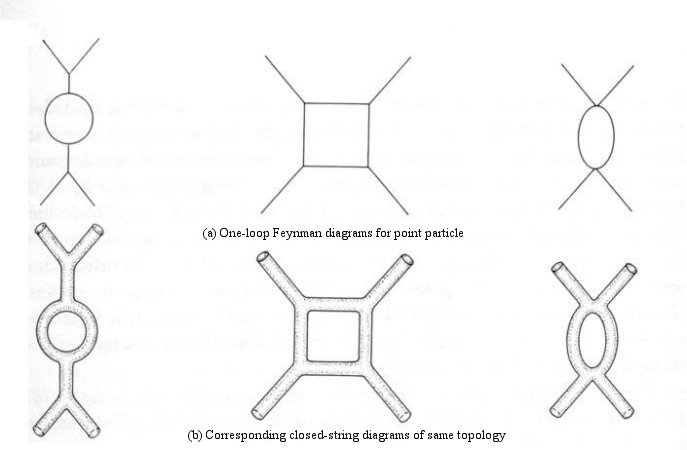
\includegraphics[width=0.7\textwidth]{graphics/strings/stringloop.jpg}
    \captionof{figure}{The correspondence between Feynman diagrams for particles and those for strings. Now there is a non-trivial topology\index{topology} involving holes etc.}
    \label{fig:stringloop}
\end{center}
Returning to amplitudes, we can't use QFT. Instead we need to revert to Feynman's path integral\index{path integral} formulation, mapping particle actions to Feynman diagrams.
\begin{equation}
\int{\mathcal{D}\phi \,\, e^{i S_{\text{particle}}}} \Longrightarrow \int{\mathcal{D}\phi \,\, e^{i S_{\text{string}}}} 
\end{equation}
This is qualitatively different to considering strings as excitations of a string field, which is much harder.
\subsection{The Relativistic Point Particle}
In physical terms, an elementary particle is one without structure, which implies that the classical action should only depend on the geometry of the worldline\index{worldline}, as well as other variables such as spin. The simplest geometric invariant is the proper time on the worldline between two points $A$ and $B$. 
\begin{equation}
I = -mc^2\int_A^B{\ud \tau}
\end{equation}
But $c\ud \tau = \sqrt{-\ud s^2} = \sqrt{-\ud x^\mu \ud x^\nu \etamn{_}}$ with $\etamn{_} = \text{diag}(-1, 1, 1, 1)$, so $c\ud \tau = \sqrt{-\dot{x}^\mu \dot{x}^\nu \etamn{_}} = \sqrt{-\dot{x}^2}\ud t$;
\begin{equation}
\label{eq:earlyaction}
\Rightarrow I[x] = -mc\int_{t_A}^{t_B}{\upd{t}\sqrt{-\dot{x}^2}}
\end{equation}
We'll see later that we are free to choose $x^0 = c\tau$, then;
\begin{equation}
I = -mc^2 \int_{t_A}^{t_B}{\upd{t}\sqrt{\left(x^0\right)^2 - \abs{\dot{\vec x}}^2}} = \int_{t_A}^{t_B}{\upd{t} \set{-mc^2 + \tfrac{1}{2}mv^2 + \mO\left(\tfrac{v^2}{c^2}\right)}}
\end{equation}
\subsubsection{Hamiltonian\index{Hamiltonian} Formalism}
Suppose we take $\mL = -mc^2 + \tfrac{1}{2}mv^2$, then we find happily that $\hamilt = \tfrac{1}{2m}\abs{\vec p}^2 + mc^2$. But suppose instead we start from $\mL = -mc\sqrt{-\dot{x}^2}$, then;
\begin{equation}
p_\mu = \frac{\del \mL}{\del \dot{x}^\mu} = \frac{mc}{\sqrt{-\dot{x}^2}}\etamn{_}\dot{x}^\nu \Rightarrow \dot{x}^\mu p_\mu = -mc \sqrt{-\dot{x}^2}
\end{equation}
But then we find that $\hamilt = 0$...the fact this vanishes is really due to the Hamiltonian generating evolution in a time variable. We can't choose a time parameter uniquely in any Lorentz invariant way, so we shouldn't expect a Hamiltonian. There is another issue though; $p^2 + (mc)^2 = 0$, so the $p^\mu$ aren't independent. As such the phase space isn't even $2n$-dimensional for some $n$. The solution to this, according to Dirac is to relax the identity ($c=1$) $p^2 + m^2 \equiv 0$ and instead impose it as a constraint via a Lagrange multiplier\footnote{We can think of $e$ as a gauge field\index{field!gauge}.} in the action:
\begin{equation}
\label{eq:lmultact}
I(x, p, e) = \int{\upd{t} \dot{x}^\mu p_\mu - \tfrac{1}{2}e(p^2 + m^2)}
\end{equation}
This directly leads to the action in \eqref{eq:earlyaction} via $\tfrac{\delta I}{\delta p} = 0 \iff p^\mu = e^{-1}\dot{x}^\mu$ leading to;
\begin{equation*}
I(x, e) = \frac{1}{2}\int{\upd{t} e^{-1}\dot{x}^2 - m^2 e}
\end{equation*}
Varying with respect to $e$, $\tfrac{\delta I}{\delta e} = 0 \iff e = \tfrac{1}{m}\sqrt{-\dot{x}^2}$ gives the result. Now, we can view \eqref{eq:lmultact} as a field theory in time with $x(t), p(t)$ interpreted as scalar fields\index{field!scalar} and $e(t)$ as a density such that under a transformation $t\pr(t) = t - \xi(t)$;
\begin{equation}
x\pr (t\pr) = x(t), \qquad p\pr(t\pr) = p(t), e\pr (t\pr) \ud t\pr = e(t) \ud t
\end{equation}
Letting $\delta x(t) = x\pr(t) - x(t)$ etc, we find;
\begin{multline}
\delta_\xi x^\mu(t) = \xi(t) \dot{x}^\mu(t) + \mO(\xi^2), \quad \delta_\xi p^\mu(t) = \xi(t)\dot{p}^\mu(t) + \mO(\xi^2), \\ \delta_\xi e(t) = \frac{\ud}{\ud t}\left(e\xi\right)
\end{multline}
Putting this into the Lagrangian; $\mL = \dot{x}^\mu p_\mu - \tfrac{1}{2}e(p^2 + m^2)$, we find that;
\begin{align*}
\mL &\rightarrow  (\dot{x}^\mu + \dot{\xi} \dot{x}^\mu + \xi \ddot{x}^\mu)(p_\mu + \xi \dot{p}_\mu) \\
& \qquad -\tfrac{1}{2}(e + \dot{e}\xi + e\dot{\xi})\left((p^\mu + \xi \dot{p}^\mu)(p_\mu + \xi \dot{p}_\mu) + m^2\right) \\
&= \mL + \dot{\xi}\left(\dot{x}^\mu p_\mu - \tfrac{1}{2}(p^2 + m^2)\right) \\
& \qquad \quad + \xi\left(\ddot{x}^\mu p_\mu + \dot{p}_\mu \dot{x}^\mu -\tfrac{1}{2}\dot{e}(p^2 + m^2) - \tfrac{1}{2}e(\dot{p}^\mu p_\mu + p^\mu \dot{p}_\mu)\right) \\
&= \mL + \frac{\ud}{\ud t}\left(\xi \mL\right)
\end{align*}
So $\mL$ changes by a total derivative and we have a general gauge invariance under one dimensional co-ordinate transformations\footnote{The group is the infinite dimensional $\text{Diff}_1$}, this validates the choice of $x^0 = ct$ we made earlier. The action $I(x, p, e)$ is invariant under a different canonical gauge transformation;
\begin{equation}
\delta_{\alpha} x^\mu = \alpha p^{\mu}, \qquad \delta_\alpha p^\mu = 0, \qquad \delta _\alpha e = \dot{\alpha}
\end{equation}
This leads to;
\begin{align*}
\delta I &= \int{\upd{t} \set{\dot{\alpha}\dot{p}^2 + \alpha \dot{p}^\mu p_\mu - \tfrac{1}{2}\dot{\alpha}(p^2 + m^2)}} \\
&= \int{\upd{t} \set{\tfrac{1}{2}\dot{\alpha}(p^2 - m^2) +  \alpha \dot{p}^\mu p_\mu}} \\
&= \int{\upd{t} \set{\frac{1}{2}\frac{\ud}{\ud t}\left(\alpha(p^2 - m^2)\right)}} \\
&= \left[\frac{1}{2}\frac{\ud}{\ud t}\left(\alpha(p^2 - m^2)\right)\right]^{t_B}_{t_A}
\end{align*}
which vanishes for suitable boundary conditions. So we have a gauge invariance\index{gauge invariance} (which is physically equivalent to the $\text{Diff}_1$ invariance). Now recall the Poisson bracket\index{Poisson bracket} on phase space is given by;
\begin{equation}
\label{eq:PB}
\set{f, g} \overset{\tiny{\text{def}}}{=}\frac{\del f}{\del x^\mu}\frac{\del g}{\del p_\mu} - \frac{\del g}{\del x^\mu}\frac{\del f}{\del p_\mu}
\end{equation}
Then, we see that,
\begin{enumerate}
\item $\alpha \set{x^\mu, \tfrac{1}{2}(p^2 + m^2)} = \alpha p^\mu = \delta_\alpha x^\mu$
\item $\alpha \set{p_\mu, \tfrac{1}{2}(p^2 + m^2)} = 0 = \delta_\alpha p_\mu$
\end{enumerate}
So the constraint function, $\tfrac{1}{2}(p^2 + m^2)$ generates the canonical gauge transformations of $x, p$. This is more general. For an arbitrary action that is time parametrisation independent (so the Hamiltonian is just a sum of Lagrange multipliers times constraint functions);
\begin{equation}
\label{eq:timeinvact}
I[q, p, \lambda] = \int{\upd{t} \set{\dot{q}^I p_I - \lambda^j \phi_j (x, p)}}
\end{equation}
Then if $\set{\phi_i, \phi_j} = f\indices{^{k}_{ij}}(x, p)\phi_k$, where $f\indices{^{k}_{ij}}(x, p)$ are structure functions on the phase space. Then $\left.\set{\phi_i, \phi_j}\right|_{\phi = 0} = 0 \,\, \forall i,j$. Then we call $\set{\phi_i}$ a first class set of constraints\index{first class!set of constraints}.\footnote{If the $f\indices{^{k}_{ij}}$ are constants then we have the full gauge group/Lie algebra structure to work with e.g. Yang-Mills theory\index{Yang-Mills theory}}

\paraskip
Now we make a few remarks on the action in \eqref{eq:timeinvact};
\begin{enumerate}
\item It is a sum of two terms; $\mL_{\text{\tiny{geometric}}} = \dot{q}^I p_I$ and $\mL_{\text{\tiny{constraints}}} = -\lambda^i \phi_i$
\item Any Lagrangian can be put into a time re-parametrisation invariant form, implying that it has no Hamiltonian (see example sheet 1)
\end{enumerate}
We discuss the geometric part of the Lagrangian first. To do so we must discuss \emph{phase space}\index{phase space}. Phase space is a symplectic manifold\index{symplectic manifold}.
\begin{definitionbox}
A \emph{symplectic manifold} is a manifold with a closed ($\ud \Omega = 0$), invertible $2$-form $\Omega$ on it. In some local co-ordinates $\set{z^A, A = 1, \ldots 2N}$, we can write;
\begin{equation}
\Omega = \tfrac{1}{2}\ud z^A \wedge \ud z^B \Omega_{AB}
\end{equation}
then the Poisson bracket\index{Poisson bracket} of functions is defined by;
\begin{equation}
\set{f, g} = \Omega^{AB}\del_A f \del_B g
\end{equation}
where $\Omega^{BA}$ is the inverse $2$-form such that $\Omega^{BA}\omega_{AC} = \delta\indices{^{B}_{C}}$.
\end{definitionbox}
There is a theorem regarding the precise form of $\Omega$;\index{Darboux theorem}
\begin{thm}[Darboux Theorem]
Suppose we have a symplectic manifold, or a phase space, with a $2$-form $\Omega$. Then there exist local\footnote{Note this is at a point \emph{and} in a neighbourhood. This is a much stronger constraint than the existence of normal co-ordinates in GR for example.} co-ordinates $\set{q^I, p_I}$. such that $\Omega = \ud p_I \wedge \ud q^I = \ud(p_I \ud q^I) \coloneqq \ud \omega$. Then;
\begin{equation}
I = \int{\omega} = \int{\upd{t} \dot{q}^I p_I} = \int{\upd{t} \mL_{\text{\tiny{geometric}}}}
\end{equation}
where the equality holds only in Darboux co-ordinates\index{co-ordinates!Darboux}. 
\end{thm}
Note that in Darboux co-ordinates, the Poisson bracket is the one quoted earlier in \eqref{eq:PB}. Furthermore, it can be shown\footnote{For example in this overflow post: \href{https://mathoverflow.net/questions/28421/the-jacobi-identity-for-the-poisson-bracket}{Jacobi Identity}} that the closed property of $\Omega$, $\ud \Omega = 0$ is equivalent to the Jacobi identity\index{identity!Jacobi}\index{Jacobi identity}. So the Poisson bracket is a Lie bracket and the space of functions on the phase space is an infinite dimensional Lie algebra. In particular, this is the algebra of \emph{symplectic diffeomorphisms}, otherwise known as \emph{canonical transformations}.\index{diffeomorphism!symplectic}\index{canonical transformation}. 

\paraskip
Using the $2$-form $\Omega$, we can define a \emph{Hamiltonian vector field}\index{vector field!Hamiltonian} associated to any function $Q(z)$ via;
\begin{equation}
\xi^{A}_Q(z) = \Omega^{AB}\del_B Q \Rightarrow \xi_Q = (\Omega^{AB} \del_B Q) \del_A
\end{equation}
From this we can see for example that $\xi_Q(f) = \set{f, Q}$. Then any co-ordinate transformation $z^A \mapsto z^A + \epsilon \xi^A_Q(z) + \mO(z^2)$ induces a change $\delta_\epsilon f$ in any other function $f(z)$;
\begin{align*}
f(z) \rightarrow f(z) + \epsilon \xi^A_Q \del_A f + \mO(z^2) &= f(z) +\epsilon \xi_Q(f) + \mO(z^2) \\
\Rightarrow \delta_\epsilon f &= \epsilon \set{f, Q}
\end{align*}
So in Darboux co-ordinates;
\begin{equation}
\delta_\epsilon q^I = \epsilon \frac{\del Q}{\del p_I}, \qquad \delta_\epsilon p_I = -\epsilon \frac{\del Q}{\del q^I}
\end{equation}
We apply this to $\mL_{\text{\tiny{geometric}}} = \dot{q}^I p_I$;
\begin{align*}
\dot{q}^I p_I &\rightarrow \dot{q}^I p_I + \epsilon \frac{\ud}{\ud t}\left(\frac{\del Q}{\del p_I}\right)p_I - \epsilon \frac{\del Q}{\del q^I}\dot{q}^I + \mO(\epsilon^2) \\
\Rightarrow \delta_\epsilon(\dot{q}^I p_I) &= \epsilon \frac{\ud}{\ud t}\left(\frac{\del Q}{\del p_I}\right)p_I - \epsilon \frac{\del Q}{\del q^I}\dot{q}^I \\
&= \epsilon \set{\frac{\ud}{\ud t}\left(\frac{\del Q}{\del p_I}p_I\right) - \dot{p}_I\frac{\del Q}{\del p_I} - \dot{q}^I\frac{\del Q}{\del q^I}} \\
&= \epsilon\set{\frac{\ud}{\ud t}\left(\frac{\del Q}{\del p_I}p_I\right) - \frac{\ud Q}{\ud t}} \\
&= \epsilon \frac{\ud}{\ud t}\left(\frac{\del Q}{\del p_I}p_I - Q\right)
\end{align*}
So $I_{\text{\tiny{geometric}}}$, or the symplectic form $\Omega$ and hence the Poisson bracket, are invariant under the algebra of canonical transformations.\footnote{Equivalently, symplectic diffeomorphisms correspond to vector fields $\xi$ such that $\mL_\xi \Omega = 0$. It can be shown that this is the same as $\xi$ being a Hamiltonian vector field establishing the correspondence between symplectic diffeomorphisms\index{diffeomorphism!symplectic} and canonical transformations. We can compare this to \emph{isometries}\index{isometry} in a metric space where we impose $\mL_\xi g = 0$.} We now let $\epsilon \rightarrow \epsilon(t)$, then we pick up an extra term in the discussion above;
\begin{equation}
\delta_\epsilon(\dot{q}^I p_I) = \dot{\epsilon}Q + \frac{\ud}{\ud t}\left(\epsilon\left(\frac{\del Q}{\del p_I}p_I - Q\right)\right)
\end{equation}
Now we move onto the constraints and apply the above expression with $Q = \epsilon^i(t)\phi_i(z)$, i.e. any set of constraints has an associated canonical transformation;
\begin{equation}
\label{eq:constrainttrans}
\delta_\epsilon(\dot{q}^I p_I) = \dot{\epsilon}^i(t) \phi_i(z) + \,\,\text{total time derivative}
\end{equation}
as well as;
\begin{equation*}
\delta_\epsilon \phi_i = \set{\phi_i, \epsilon^j \phi_j} = \epsilon^j (t) \set{\phi_i, \phi_j} = \epsilon^j f\indices{^{k}_{ij}}\phi_k
\end{equation*}
where the last equality only holds if the constraints are first class\index{first class constraints}. Plugging this into the full Lagrangian;
\begin{align*}
\delta \mL_{\text{\tiny{geometric}}} + \delta \mL_{\text{\tiny{constraints}}} &= \dot{\epsilon}^k \phi_k - \lambda^i \epsilon^j f\indices{^{k}_{ij}}(z)\phi_k - \delta \lambda^k \phi_k \\
&= \left(\dot{\epsilon}^k + \epsilon^i \lambda^j f\indices{^{k}_{ij}}(z) - \delta \lambda\right) \phi_k
\end{align*}
So $\delta \mL_{\text{\tiny{geometric}}} + \delta \mL_{\text{\tiny{constraints}}} = 0$ if;
\begin{equation}
\delta \lambda^k = \dot{\epsilon}^k + \epsilon^i \lambda^j f\indices{^{k}_{ij}}(z)
\end{equation}
This is the transformation of a gauge potential in one dimension. We will find for a string that the structure functions really are constant, so we have a non-abelian gauge theory.\index{gauge theory!non-abelian}. Thus we see that any set of constraints has an associated gauge transformation.
\subsubsection{Noether's Theorem}
As always, a continuous symmetry of the action leads to a constant of the motion, the \emph{Noether charge}\index{Noether charge}. Now let $\epsilon \ll 1$ be a parameter and under a given transformation, $\delta_\epsilon I = 0$, by the definition of a symmetry. If $\epsilon \rightarrow \epsilon(t)$, then we know that;
\begin{equation*}
\delta_\epsilon I = \int{\upd{t}\dot{\epsilon} Q}
\end{equation*}
for some $Q(z)$. But the equations of motion insist that this must vanish, so ;
\begin{equation*}
0 = \int{\upd{t}\dot{\epsilon}Q} = -\int{\upd{t}\epsilon \dot{Q}} + [\epsilon Q]
\end{equation*}
Hence if $\epsilon$ vanish at the end points, we find $\dot{Q} = 0$, where $Q$ is the Noether charge. Furthermore, given $Q$ we can find the symmetry transformation via;
\begin{equation}
\label{eq:symm}
\delta_\epsilon f = \epsilon\set{f, Q}
\end{equation}
It might be that the right hand side of \eqref{eq:symm} vanishes. In this case $Q$ is not a Noether charge, instead it is a topological charge\index{topological charge}.

\paraskip
Now we return to the 1-particle action,
\begin{equation*}
I = \int{\upd{t} \set{\dot{x}^m p_m -\tfrac{1}{2}(p^2 + m^2)}}
\end{equation*}
The first term is invariant under the infinite dimensional algebra of canonical transformations. The second term breaks this symmetry however and is only invariant if $p^2 = \etamn{^}p_\mu p_\nu$ is also. This is equivalent to $\etamn{^}$ being invariant. But these are precisely the Lorentz transformations\index{Lorentz transformation}, or more generally the Poincar� group\index{group!Poincar�}. Infinitesimally, we have $\Lambda\indices{^{\mu}_{\nu}} = \delta\indices{^{\mu}_{\nu}} + \omega\indices{^{\mu}_{\nu}} + \mO(\omega^2)$.
\begin{enumerate}
\item $x^\mu \mapsto \Lambda\indices{^{\mu}_{\nu}}x^\nu + a^\mu \Rightarrow \delta x^\mu = a^\mu + \omega\indices{^{\mu}_{\nu}}x^\nu$
\item $p_\mu \mapsto \Lambda\indices{_{\mu}^{\nu}}p_\nu \Rightarrow \delta p_\mu = \omega\indices{_{\mu}^{\nu}}p_\nu$
\end{enumerate}
This must lead to $\delta I = 0$ as claimed in the paragraph above. In accordance with Noether's theorem\index{theorem!Noether}, to find the constants of the motion, we promote $a, \Lambda$ to functions of time, $a(t), \Lambda(t)$ so that $\dot{x}^\mu \mapsto \dot{a}^\mu + \omega\indices{^{\mu}_{\nu}}\dot{x}^\nu + \dot{\omega}\indices{^{\mu}_{\nu}}x^\nu$. Then we find;
\begin{equation}
\delta I = \int{\upd{t}\set{\dot{a}^\mu \mathcal{P}_\mu + \tfrac{1}{2}\dot{\omega}_{\mu\nu}\mathcal{J}^{\mu\nu}}}
\end{equation}
where $\mathcal{P}_\mu = p_\mu$ and $\mathcal{J}^{\mu\nu} = x^\mu p^\nu - x^\nu p^\mu$.\footnote{Note that these are also gauge invariant under the canonical transformations $\delta_\alpha x^\mu = \alpha p^\mu, \delta_\alpha p_\mu = 0$, so gauge fixing does not break the symmetries.}.
\begin{definitionbox}
In general, gauge invariances generated via the transformations in \eqref{eq:constrainttrans} by $\epsilon^j \phi_j(z)$ can be fixed\index{gauge fixing} by imposing $\chi^i (z) = 0$, on the condition that;
\begin{equation}
\delta_\epsilon \chi^i = \set{\chi^i, \phi_j}\epsilon^j = 0 \iff \epsilon^j = 0
\end{equation}
A necessary and sufficient condition for this is that $\det\set{\chi^i, \phi_j} \neq 0$.
\end{definitionbox}
As an example of this, consider $\chi = x^0(t) - t$, known as the \emph{temporal gauge}\index{gauge!temporal}, with $\phi = \tfrac{1}{2}(p^2 + m^2)$. Then;
\begin{equation}
\left.\set{\chi, \phi}\right|_{\phi = 0} = \left.p_0 \right|_{\phi = 0} = \mp \sqrt{\abs{\vec p}^2 + m^2} \neq 0
\end{equation}
Then $\dot{x}^\mu p_\mu \mapsto \dot{\vec x} \cdot \vec p + p_0 = \dot{\vec x} \cdot \vec p - p^0$. Then the gauge fixed action is;
\begin{equation}
I = \int{\upd{t} \dot{\vec x}\cdot \vec p - \hamilt}, \qquad \hamilt = \pm\sqrt{\abs{\vec p}^2 + m^2}
\end{equation}
where we have identified the Hamiltonian with $p^0$. This is still Poincar� invariant, even though it doesn't necessarily appear to be. Furthermore, we now have a Hamiltonian, which depends on the gauge choice, although in general Hamiltonians are related by a canonical transformation\index{canonical transformation}.

\paraskip
Suppose we move into another gauge, the \emph{light-cone gauge}\index{gauge!light-cone}. Here we define,
\begin{equation}
x^{\pm} = \tfrac{1}{\sqrt{2}}(x^1 \pm x^0), \quad p_{\pm} = \tfrac{1}{\sqrt{2}}(p_1 \pm p_0)
\end{equation}
Then we define the \emph{transverse} $(d-2)$-vectors, $\vec x = (x^2, \ldots, x^{d-1}), \vec p = (p_2, \ldots, p_{d - 1})$. In the $\set{x^+, x^-, \vec x}$ co-ordinates, the metric is;
\begin{multline}
\ud s^2 = 2\ud x^+ \ud x^- + \ud \vec x \cdot \ud \vec x \\ \Rightarrow \eta^{+-} = \eta^{-+} = \eta_{+-} = \eta_{-+} = 1, \eta^{II} = \eta_{II} = \delta_{II}
\end{multline}
This implies $p^{+} = p_{-}, p^{-} = p_{+}$. So the geometric part of the Lagrangian is;
\begin{equation}
\mL_{\text{\tiny{geometric}}} = \dot{x}^\mu p_\mu = \dot{x}^+ p_+ + \dot{x}^- p_- + \dot{x}^I p_I \qquad \left(I = 1, \ldots, (d-2)\right)
\end{equation}
and the constraint part is;
\begin{equation}
\mL_{\text{\tiny{constraint}}} = -e\set{p_+ p_- + \tfrac{1}{2}(\abs{\vec p}^2 + m^2)}
\end{equation}
In the light cone gauge, we set $x^+(t) = t$ so that $\chi = x^+ (t) - t$. Then;
\begin{equation}
\left.\set{\chi, \phi}\right|_{\phi = 0} = \left.p_-\right|_{\phi = 0} \Rightarrow -p_+ = \frac{\abs{\vec p}^2 + m^2}{2p_-}
\end{equation}
So that we have $\dot{x}^\mu p_\mu = \dot{x}^- p_- + \dot{\vec x} \cdot \vec p + p_+$ since $\dot{x}^+ = 1$ in the light-cone gauge, then the light cone action is;
\begin{equation}
I_{\text{\tiny{light-cone}}} = \int{\upd{t} \set{\dot{x}^- p_- + \dot{\vec x} \cdot \vec p - \hamilt}}, \qquad \hamilt = \frac{\abs{\vec p}^2 + m^2}{2p_-}
\end{equation}
This is well-defined provided $p_- \neq 0$. From the Lagrangian, the canonical momentum $p_- \sim \dot{x}^+$, so provided we don't have a curve such as the blue one shown in \autoref{fig:lightcone} where $\dot{x}^+ = 0$. In this case, we can no longer use $x^+$ as a parameter.
\begin{mygraphic}{strings/lightcone}{0.5}{On the timelike curve (red), $x^0$ is an unambiguous time parameter choice. On the other hand, for the blue curve, we have $p_- = 0$ in the upper left quadrant, which violates our condition.}{lightcone}\end{mygraphic}
\subsection{Quantization}
In the temporal gauge, we take a positive energy so that the Lagrangian is;
\begin{equation}
\mL = \dot{\vec x}\cdot \vec p - \sqrt{\abs{\vec p}^2 + m^2}
\end{equation}
with canonical PB relations, $\set{x^i, p_j} = \delta\indices{^{i}_{j}}$. To quantise, we promote the co-ordinates to operators, and let $\set{\,\,,\,\,\,} \mapsto \tfrac{-i}{\hbar} [\,\,,\,\,\,]$ to get the canonical commutation relations $[\hat{x}^i, \hat{p}_j] = i\hbar \delta\indices{^{i}_{j}}$. In the $x$-space representation, $\hat{x}$ is diagonal and $\hat{p}_i = -i\hbar \del_i$, to that $\abs{\hat{p}}^2 = \hbar^2 \nabla^2$. Then the Schr{\"o}dinger equation\index{equation!Schr{\"o}dinger} becomes;
\begin{align*}
\hat{\hamilt} \psi(\vec x, t) = \sqrt{-\hbar^2 \nabla^2 + m^2} \psi &= i\hbar \del_t \psi \\
\Rightarrow (-\hbar^2 \nabla^2 + m^2)\psi &= -\hbar^2 \del_t^2 \psi \\
\Rightarrow \left(\Box - \left(\frac{m}{\hbar}\right)^2\right)\psi &= 0
\end{align*}
Importantly, we end up with a manifestly Lorentz invariant equation of motion, even though the intermediate Lagrangian was not manifestly Lorentz invariant. This had to be the case of course, but we would like to keep the manifest invariance throughout:
\subsubsection{Covariant Quantisation}
We start from the Lorentz invariant action;
\begin{equation*}
I = \int{\upd{t}\set{\dot{x}^\mu p_\mu - \tfrac{1}{2}e(p^2 + m^2)}}
\end{equation*}
Now we take a different approach;
\begin{enumerate}
\item First quantise $\set{\,\,,\,\,\,} \mapsto [\,\,,\,\,\,]$ as if there was no constraint (i.e. for all the variables, even $\hat{x}^0$ which is not really an operator).
\item Because of the gauge invariance\index{gauge invariance} there are unphysical states in the Hilbert space\index{Hilbert space}. We need to remove these with a constraint. The mass-shell constraint encodes the full dynamics of the particle, so we now impose this in the quantum theory as the physical state condition;
\begin{equation}
(\hat{p}^2 + m^2) \ket{\psi} = 0 \iff \left(\Box - \left(\frac{m}{\hbar}\right)^2\right)\psi(x) = 0
\end{equation}
\end{enumerate}
so we recover the Klein-Gordon equation\index{equation!Klein-Gordon} without manifestly breaking the Lorentz invariance.
\newpage
\section{The Nambu-Goto String}
To move from a particle to a string, we move from a \emph{worldline}\index{worldline} to a \emph{worldsheet}\index{worldsheet} parametrised by $\sigma^{\mu} \coloneqq (t, \sigma)$. For an open string\index{string!open} we simply have $\sigma \in \RR$, however for a closed string\index{string!closed} we identify $\sigma \sim \sigma + 2\pi$.  We can envision this $2$-dimensional surface (or an $n$-dimensional surface in the case of a brane\index{brane}) embedded in a $d$-dimensional spacetime. We can encode this embedding by considering the mapping between the worldsheet and the spacetime with scalar fields $X^{m}(\sigma^\mu)$ on the worldsheet. There is an induced metric, $g$, on the worldsheet which arises via the relation;
\begin{equation}
g_{\mu\nu} = \del_{\mu}X^{m}\del_{\nu}X^{n}\eta_{mn}
\end{equation} 
The simplest density we can consider is $\sqrt{-\det g}$, integrating this over the world sheet gives the Nambu-Goto action\index{Nabu-Goto!action}\index{Nambu-Goto!string};\footnote{We don't include curvature scalars at this stage as each of these terms would introduce an additional length scale. The point of string theory is that we are considering a fundamental string which by definition doesn't have any additional structure.}
\begin{equation}
I_{\text{NG}} = -T\int{\ud \mathcal{A}} = -T\int{\ud t \upd{\sigma}\sqrt{-\det g}}
\end{equation}
As in the point particle case, this geometric action is invariant under a very broad class of $2$-dimensional diffeomorphisms\index{diffeomorphism};
\begin{equation}
\sigma^\mu \mapsto \sigma^\mu + \xi^{\mu}(t, \sigma)
\end{equation}
Then we see that $\delta_{\epsilon}X^{m}= \xi^{\mu}\del_\mu X^{m}$, which implies that $\delta_{\epsilon}(-\det g) = \del_{\mu}\left(\xi^{\mu}\sqrt{-\det g}\right)$ and hence $\delta I = 0$. The equation of motion is the found by varying $X$;
\begin{equation}
\frac{\delta I}{\delta X^{\mu}} = 0 \Rightarrow \del_\mu\left(\sqrt{-\det g}g^{\mu\nu}\del_\nu X^{m}\right) = 0
\end{equation}
which we will derive later in the course.
\subsection{Hamiltonian Formalism}
We have $g_{\mu\nu} = \del_\mu X \cdot \del_\nu X$. Now let $\dot{X} = \del_t X$ and $X\pr = \del_\sigma X$, then we find explicitly;
\begin{equation}
g_{\mu\nu} = \twobytwo{\dot{X}^2}{\dot{X}\cdot X\pr}{\dot{X}\cdot X\pr}{(X\pr)^2}
\end{equation}
so that the action becomes;
\begin{equation}
I_{\text{NG}} = -T\int{\upd{t}\int{\upd{\sigma} \sqrt{-\dot{X}^2 (X\pr)^2 + (\dot{X}\cdot X\pr)^2}}}
\end{equation}
We define the Lagrangian density\index{Lagrangian!density} to be the square root. Then we define the associated momentum density\index{momentum density};
\begin{equation}
P_m(t, \sigma) = \frac{\del \mL}{\del \dot{X}^{m}(t, \sigma)} = \frac{T}{\sqrt{-\det g}}\left(\dot{X}_{m}(X\pr)^2 - X\pr_m (\dot{X}X\pr)\right)
\end{equation}
Then the Hamiltonian density\index{Hamiltonian!density} is;
\begin{align*}
\hamilt &\coloneqq \dot{X}^{m}P_m - \mL \\
&= \frac{T}{\sqrt{-\det g}}\set{\dot{X}^2\left(X\pr\right)^2 - \left(\dot{X}\cdot X\pr\right)^2} - \mL \\
\Rightarrow \hamilt &= 0
\end{align*}
We can also show that;
\begin{enumerate}
\item $(X\pr)^{m}P_m = X\pr \cdot \dot{X}(X\pr)^2 - (X\pr)^2\dot{X}\cdot X\pr = 0$
\item $P^2 + (TX\pr)^2 = 0$
\end{enumerate}
Then applying these as constraints we write the phase space action;\footnotemark
\begin{equation}
I(X, P, e, u) = \int{\upd{t}\int{\upd{\sigma}\set{\dot{X}^{m}P_m - \tfrac{1}{2}e\left(P^2 + (TX\pr)^2\right) - uX\pr \cdot P}}}
\end{equation}
\footnotetext{
We should check that this reproduces the geometric action we had previously.
\begin{equation*}
\frac{\delta I}{\delta P} = 0 \Rightarrow P = e^{-1}D_t X = e^{-1}(\dot{X} - u X\pr)
\end{equation*}
Substituting this in we find;
\begin{align*}
I[X, e, u] &= \tfrac{1}{2}\int{\upd{^2 \sigma} \set{e^{-1}(D_t X)^2 - e(T X\pr)^2}} \\
&= \tfrac{1}{2}\int{\upd{^2 \sigma}\set{e^{-1}\left(\dot{X}^2 - 2u\dot{X}X\pr + u^2 (X\pr)^2\right) - e(TX\pr)^2}}
\end{align*}
where $(D_t X) = \dot{X} - u X\pr$. Then;
\begin{align*}
\frac{\delta I}{\delta u} &= 0 \Rightarrow u = \frac{\dot{X}X\pr}{(X\pr)^2} \\
\Rightarrow I[X, e] &= \frac{1}{2}\int{\upd{^2\sigma}e^{-1}\left(\dot{X}^2 - \frac{2 (\dot{X}X\pr)^2}{(X\pr)^2} + \frac{(\dot{X}X\pr)^2}{(X\pr)^2}\right) - e(TX\pr)^2} \\
&= \frac{1}{2}\int{\upd{^2 \sigma}e^{-1}\frac{\det g}{(X\pr)^2} - e(TX\pr)^2}
\end{align*}
Finally, differentiating with respect to $e$;
\begin{equation*}
\frac{\delta I}{\delta e} = 0 \Rightarrow e = \frac{1}{T(X\pr)^2}\sqrt{-\det g}
\end{equation*}
Substituting in gives the result.
}
There is an alternative form to this phase space action\index{action!phase space}. Note that the constraints are equivalent to a more symmetric choice;
\begin{equation}
\hamilt_{\pm} = 0, \qquad \hamilt_{\pm} = \frac{1}{4T}(P \pm TX\pr)^2
\end{equation}
so we may instead work with;
\begin{equation}
I = \int{\upd{^2 \sigma} \set{\dot{X}^{m}P_{m} - \lambda^{-}\hamilt_{-} - \lambda^{+}\hamilt_{+}}}
\end{equation}
where $\lambda^{\pm} = Te \pm u$. This is a useful parametrisation since the $\lambda^{\pm}$ are dimensionless. Now for any functionals $F[X(\sigma^\mu), P(\sigma^{\mu})], G[X(\sigma^\mu), P(\sigma^{\mu})]$ the Poisson bracket\index{Possion bracket} is defined by;
\begin{equation}
\set{F, G} = \oint{\upd{\sigma}\left[\frac{\delta F}{\delta X^{m}(\sigma^{\mu})}\frac{\delta G}{\delta P_{m}(\sigma^{\mu})} - \frac{\delta G}{\delta X^{m}(\sigma^{\mu})} \frac{\delta F}{\delta P_{m}(\sigma^{\mu})}\right]}
\end{equation}
This implies that $\set{X^{m}(\sigma^{\mu}), P_{n}\left((\sigma\pr)^{\mu}\right)} = \delta\indices{^{m}_{n}}\delta(\sigma - \sigma\pr)$. A very lengthy calculation implies;
\begin{enumerate}
\item $\set{\hamilt_{+}(\sigma), \hamilt_{+}(\sigma\pr)} = \left(\hamilt_{+}(\sigma) + \hamilt_{+}(\sigma\pr)\right)\delta\pr(\sigma - \sigma\pr)$
\item $\set{\hamilt_{-}(\sigma), \hamilt_{-}(\sigma\pr)} = \left(\hamilt_{-}(\sigma) + \hamilt_{-}(\sigma\pr)\right)\delta\pr(\sigma - \sigma\pr)$
\item $\set{\hamilt_{+}(\sigma), \hamilt_{-}(\sigma\pr)} = 0$
\end{enumerate}
These are a set of first class constraints\index{first class constraint} with constant structure factors, so the constraints span an infinite dimensional\footnote{For each $\sigma$} Lie algebra\index{Lie!algebra}. We also know that $-\hamilt_{-}$ and $\hamilt_{+}$ have the same algebra and hence the full algebra is the sum of two isomorphic algebras.\footnotemark
\footnotetext{
In fact it is $\text{Diff}_1^{(+)}\oplus \text{Diff}_2^{(-)} \subset \text{Diff}_2$, so we have a much simpler group of transformations that the full gauge invariance. Everything else in $\text{Diff}_2$ is `trivial' - the gauge invariances have no physical effect. Interestingly, $\text{Diff}_1^{(+)} \oplus \text{Diff}_1^{(+)}$ is in fact \emph{conformal invariance}\index{conformal invariance}.
}
\paraskip
For any functional, $F[X, P]$, there is a canonical transformation generated by the constraints $\hamilt_{\pm}$;
\begin{equation}
\label{eq:cantran}
\delta_{\xi}F[X, P] = \set{F, \oint{\upd{\sigma}\xi^+ \hamilt_+ + \xi^- \hamilt_-}}
\end{equation}
where $\xi^{\pm}(t, \sigma)$ are parameters of the gauge transformation\index{gauge transformation}. Then we can show;
\begin{align*}
\delta_\xi X^{m} &= \tfrac{1}{2T}\xi^- (P - TX\pr)^m + \tfrac{1}{2T}\xi^+ (P + TX\pr)^m \\
\delta_\xi P^{m} &= -\tfrac{1}{2}\left(\xi^{-}(P - TX\pr)\right)^{\prime}_m + \tfrac{1}{2}\left(\xi^{+}(P + TX\pr)\right)^{\prime}_m
\end{align*}
Note that $\delta_{\xi^-}(P + TX\pr) = \delta_{\xi^+}(P - TX\pr) = 0$ and hence $\delta_{\xi^{+}}\hamilt_- = \delta_{\xi^{-}}\hamilt_+ = 0 \iff \set{\hamilt_+(\sigma), \hamilt_- (\sigma\pr)} = 0$.\footnote{Note that this follows because of the definition in \eqref{eq:cantran}} In fact, we also have that 
\begin{equation}
\delta_\xi \hamilt_{\pm} = \pm (\xi^{\pm})\pr \hamilt_{\pm} \pm (\xi^{\pm}\hamilt_{\pm})\pr
\end{equation}
and;
\begin{equation}
\delta_\xi (\dot{X}^{m}P_m) = \dot{\xi}^{+}\hamilt_+ + \dot{\xi}^{-}\hamilt_- + \frac{\ud}{\ud t}(\cdots)
\end{equation}
It is then easy to show that $\delta I = 0$ if the gauge fields $\lambda^{\pm}$ transform as;
\begin{align}
\delta\lambda^{-} &= \dot{\xi}^{-} + \lambda^{-}(\xi^{-})\pr - \xi^{-}(\lambda^{-})\pr \\
\delta\lambda^{+} &= \dot{\xi}^{+} - \lambda^{+}(\xi^{+})\pr + \xi^{+}(\lambda^{+})\pr
\end{align}
\subsection{Symmetries of the Nambu-Goto Action}
As for particles, we can consider $X^{m}, P^{m}$ transforming under a Poincar� transformation;
\begin{equation}
\delta X^{m} = a^{m} + \omega\indices{^{m}_{n}}X^{n}, \quad \delta P_m = \omega\indices{_{m}^{n}}P_n
\end{equation}
Then the Noether charges for the closed string are;
\begin{equation}
\mathcal{P}_m = \oint{\upd{\sigma} P_m}, \quad \mathcal{J}^{mn} = \oint{\upd{\sigma}(X^{m}P^{n} - X^{n}P^{m})}
\end{equation}
For an open string on the other hand, we have the action;
\begin{equation}
I = \int{\ud{t}\int{\upd{\sigma}\set{\dot{X}^{m}P_{m} - \tfrac{1}{2}e(P^2 + (T X\pr)^2) - uX^{\prime m}P_m}}}
\end{equation}
Then $\delta I$ has a boundary term;
\begin{multline}
\delta I = \int{\ud t}\int_0^\pi{\upd{\sigma}} \delta P_m (D_t X^m - eP^m) - \tfrac{1}{2}\delta e\left(P^2 + (TX\pr)^2\right) - \delta u X\pr P \\ + \delta X^m \left(- \dot{P}_m + T^2 (eX\pr)\pr + (uP_m)\pr\right) - \left(\left(T^2(eX\pr) + uP\right)\cdot \delta X\right)\pr
\end{multline}
So $\delta I = 0$ (with the constraints applied) gives us the Euler-Lagrange equations and the boundary conditions;
\begin{enumerate}
\item \emph{Euler-Lagrange Equations:}
\begin{equation}
D_t X^m = eP^m, \qquad \dot{P}_m = (T^2 e X\pr + uP)\pr
\end{equation}
Note that the second equation already gives us the conservation of $\mathcal{P}_m$ in the closed string case; it is a total derivative, so when it is integrated round a loop, it vanishes trivially.
\item \emph{Boundary Conditions:}
\begin{equation}
\left[\left(T^2(eX\pr) + uP\right)\cdot \delta X\right]^\pi_0 = 0
\end{equation}
\end{enumerate}
We now should assume that $X^0$ is not fixed at $\sigma = 0, \pi$. This is simply because the ends of the strings have world lines. Fixing $X^0$ is equivalent to saying the end-points only exist at one time. So instead it must be that;
\begin{equation}
\left[T^2 (eX^{0\prime}) + uP_0\right]_{\sigma = 0, \pi} = 0
\end{equation}
But, $P^0 = e^{-1}D_t X^0$ so $P^0$ is a free variable of $X^0$. Hence $\set{X^0, P_0}$ are free at the endpoints\footnote{Assuming $e \neq 0$}. Then it must be the case that $eX^{\prime 0}$ and $uP_0$ vanish independently at the endpoints, so;
\begin{equation}
u(\sigma = 0, \pi) = (X^0)\pr(\sigma = 0, \pi) = 0
\end{equation}
This leaves us with the boundary condition;
\begin{equation}
\left.\vec{X}\pr \cdot \delta \vec{X}\right|_{\text{ends}} = 0
\end{equation}
This gives us two choices;
\begin{itemize}
\item We can impose \emph{Dirichlet Boundary Conditions}\index{boundary conditions!Dirichlet} where we fix $\delta \vec{X} = 0$\footnote{Despite the observation that the only way to choose Lorentz invariant boundary conditions is to enforce Neumann boundary conditions, these do play a role in the construction of $D$-branes\index{D-brane}. The issue with Dirichlet conditions is that momentum can propagate along the string and `leak' out of the ends. This can be resolved if we attach the string to another object that the momentum flows into, in directions transverse to the string. This is the so called $D$-brane.}
\item Or we can impose \emph{Neumann Boundary Conditions}\index{boundary conditions!Neumann} where we fix $\vec{X}\pr = 0$
\end{itemize}
We should do this for each field at each end, but we have taken Neumann boundary conditions for $X^0$ so the only Lorentz invariant choice is to have Neumann conditions for all the space components. These are then the standard conditions and give us for example;\footnotemark
\footnotetext{
By the mass-shell condition $P^2 + (TX\pr)^2 = 0$ applying our boundary conditions, we see that $P^2 = 0$ on the ends of the string. Then $\left.P^2\right|_{\text{ends}} = \left.e^{-1}D_t X\right|_{\text{ends}} = e^{-1}\dot{X}$ so $\dot{X} = 0$ at the ends of the string, i.e. the ends travel at the speed of light.
}
\begin{equation}
\dot{\mathcal{P}}_m = \int_0^{\pi}{\upd{\sigma}\dot{P}_m} = \left[T^2 eX\pr_m + uP_m\right]_0^{\pi} = 0
\end{equation}
\subsection{Monge Gauge}
We make the very natural choice $X^0(t, \sigma) = t, X^1(t,  \sigma) = \sigma$\footnote{We can do this at least locally} then the constraints become;
\begin{equation*}
X^{\prime m}P_m = 0 = P_1 + \vec{X}\pr \cdot \vec{P} \Rightarrow P_1 = -\vec{X}\pr \cdot \vec{P}
\end{equation*}
where we have taken $\set{X^2, \ldots} \coloneqq \vec{X}$, and;
\begin{align*}
0 &= -P_0^2 + P_1^2 + \abs{\vec{P}}^2 + T^2(1 + \abs{\vec{X}}^2) \\
\Rightarrow P_0 &= \pm T\sqrt{1 + \abs{\vec{X}\pr}^2 + T^2\left(\abs{\vec{P}}^2 + (\vec{X}\pr\cdot\vec{P})^2\right)} 
\end{align*}
So that;
\begin{equation}
I = \int{\ud t\oint{\upd{\sigma}\set{\dot{\vec{X}}\cdot \vec{P} - \hamilt}}}
\end{equation}
where $\hamilt = P^0 \Rightarrow H = \pm T\oint{\upd{\sigma} \sqrt{1 + \abs{\vec{X}\pr}^2 + \cdots}}$. If we take $\left.\vec{P}\right|_{t = t_0}$\footnote{We assume here a moment at which the entire string is simultaneously at rest; such a moment exists only for very special string configurations, but these suffice for the argument.}, then;
\begin{align*}
H_{t = t_0} &= T\oint{\upd{\sigma}(1 + \abs{\vec{X}\pr}^2)^{\tfrac{1}{2}}} \\
&= T\oint{\upd{\sigma}\left(\abs{X_1\pr}^2 + \abs{\vec{X}\pr}^{2}\right)^{\tfrac{1}{2}}} \\
&= T\oint{\sqrt{\left.\ud s^2\right|_{\text{induced}}(t = t_0)}} \\
&= T \oint{\ud l} = T \times \text{ length of the string}
\end{align*}
So the energy density\index{energy density} $H = T$ and hence the Nambu-Goto\index{Nambu-Goto string} string is ultra-relativistic, it saturates the bound $\rho \leq c^{-2}T$. 









%\end{multicols*}
\newpage
\label{sfp}
\begin{chapterbox}
\vspace{-60pt}
\chapter{Symmetries, Fields and Particles}\label{chap:sfp}
\vspace{-30pt}
\centering\normalsize\textit{Michaelmas Term 2017 - Professor N. Dorey}
\end{chapterbox}
\vspace{20pt}
%\begin{multicols*}{2}
\minitoc
\newpage
\section{Introduction}
\subsection{Mathematical Formulation}

\begin{definitionbox}
A Lie Group\index{group!Lie}, $\group$, is a group which is also a smooth manifold\index{manifold}. Each point on the manifold corresponds to an element of the group.
\end{definitionbox}
We need the group and manifold structure to be compatible, requiring continuity and smoothness for multiplicative and inverse properties of the group. This ensures $\group$ is almost entirely determined by the behaviour near $e$, i.e. by tangent vectors, $V \in \mathcal{T}_e(\group)$. $\mathcal{T}_e(\group)$ is equipped with a Lie Bracket:
$$\left[\,\,\, , \,\,\,\right]:\mathcal{T}_e(\group)\times \mathcal{T}_e(\group) \rightarrow \mathcal{T}_e(\group)$$
which defines a Lie Algebra, $\mathcal{L}(\group)$. \boxed{\textbf{I.i}} \boxed{\textbf{I.ii}} \boxed{\textbf{I.iii}}

\subsection{Simple, Complex Lie Algebras}

\subsubsection{Cartan Classification}

\begin{definitionbox}
All \emph{finite dimensional semi-simple} Lie Algebras over $\mathbb{C}$ either belong to four infinite families: $A_n, B_n, C_n, D_n$ with $n \in \mathbb{N}$, or are one of the five exceptional cases: $E_6, E_7, E_8, G_2, F_4$.
\end{definitionbox}
In quantum mechanics, the states of the system are states in some Hilbert space, $\mathfrak{H}$. To understand the symmetries, we just need to understand the commutators of the symmetry, e.g. $\left[ \hat{L}_i , \hat{L}_j \right] = i\epsilon\indices{_{ijk}} \hat{L}_k$ which is the algebra of $\mathcal{L}\left(\textrm{SO}(3)\right)$. The operators often act on some finite dimensional vector space, $\mathcal{H}$, the \emph{representation space}. For an electron, this is $\mathcal{H} = \mathbb{C}^2$, the operators then lie in a 2-dimensional representation of $\mathcal{L}\left(\textrm{SO}(3)\right)$: the Pauli matrices, $\sigma_i$ which preserves the Lie bracket structure. If the system is invariant under this symmetry, then we have $\left[ \mathcal{H} , \hat{L}_i \right] = 0$ and thus all the states in some irreducible representation have the same energy. This can be generalised:
\begin{definitionbox}
Degeneracies in the spectrum of a quantum system are determined by irreducible representations of a global symmetry.
\end{definitionbox}
\noindent Global symmetries split into two classes (note that these are distinct from gauge symmetries):
\begin{itemize}
\item \emph{Spacetime symmetries:} rotational, Lorentz, Poincar�, supersymmetry (?)
\item \emph{Internal symmetries:} electric charge, flavour, baryon number
\end{itemize}

\subsection{Gauge Symmetry}

In contrast, a gauge symmetry\index{symmetry!gauge} is a redundancy in the mathematical description, for example in the phase of the wavefunction, $\psi \rightarrow e^{i\delta}\psi$, or in Electromagnetism, $A_{\mu} \rightarrow A_{\mu} + \partial_{\mu}\chi$. The Standard Model is a non-Abelian gauge theory with $\group_{\textrm{SM}}=\textrm{SU}(3) \times \textrm{SU}(2) \times \textrm{U(1)}$.
\newpage
\section{Lie Groups}

\subsection{Manifolds}

We can cover a manifold of dimension $n$ with one-to-one functions called \emph{charts}\index{chart}, $\phi_{\alpha} : U_{\alpha} \rightarrow V_{\alpha} \subset \mathbb{R}^n$.

\begin{thm}\label{thm:manifold}
Suppose we have a map $F : \mathbb{R}^n \rightarrow \mathbb{R}^m$ where $m<n$ with co-ordinates $\left\{ x_i \right\}$, $i = 1, \ldots, n$ and $\left\{ w_{\alpha} \right\}$, $\alpha = 1, \ldots, m$. A manifold $\mathcal{M}$ is a solution to the equations:
\begin{dmath}
F_{\alpha}\left( x_1, \ldots, x_n \right) \hiderel{=} w^{(0)}_{\alpha} \hiderel{\iff} \mathcal{M} \hiderel{=} F^{-1}\left( \bm{w}^{(0)} \right) = \left\{ \bm{x} \hiderel{\in} \mathbb{R}^n \hiderel{:} F_{\alpha}\left( \bm{x} \right) \hiderel{=} w^{(0)}_{\alpha} \right\}
\end{dmath}
Now define the Jacobian\index{Jacobian} matrix:
\begin{equation}
\mathfrak{J}\indices{_{\alpha i}}=\frac{\partial F_{\alpha}}{\partial x_i}
\end{equation}
Then, if $\mathfrak{J}$ has full rank, $m$, $\mathcal{M}$ is a manifold of dimension $(n-m)$.
\end{thm}

\subsection{Back to Lie Groups}

The dimension of $\group$, $\dim \group$, is the dimension of the group manifold $\mathcal{M}\left( \group \right)$. We can introduce co-ordinates $\left\{ \theta^i \right\}$, $i = 1, \ldots, \dim \group$ in some co-ordinate patch containing the identity $e \in \group$. Then the group elements depend continuously on $\bm{\theta}$, $g = g(\bm{\theta})$. Then:

\begin{enumerate}
\item \emph{Group Multiplication:} corresponds to a smooth map from $\group \times \group \rightarrow \group$. The co-ordinates
$$\phi^i = \phi^i \left( \bm{\theta}, \bm{\theta}' \right)$$
are differentiable and continuous. Then $g(0) = e \Rightarrow \phi^{i} \left( \bm{\theta}, 0 \right) = \theta^{i}, \,\,\, \phi^{i} \left( 0, \bm{\theta}' \right)  = \theta^{\prime i}$.
\item \emph{Group Inversion:} This defines a smooth map from $\group \rightarrow \group$ where the co-ordinates:\footnote{To be a bit more precise, consider a map $f: \mM(\group) \rightarrow \mM(\group)$ that induces a map $\theta \mapsto \tilde{\theta}$. Suppose we have charts $\phi$ and $\tilde{\phi}$ on the domain space and the image space respectively, then the statement that $\theta \mapsto \tilde{\theta}$ is a smooth map is really the property that $\tilde{\phi}^{-1} \circ f \circ \phi$ is a smooth map from $\RR^{n}$ to $\RR^{n}$ where $\dim \mM(\group) = n$.}
$$\tilde{\theta}^i = \tilde{\theta}^i\left( \bm{\theta} \right)$$

\noindent are continuous and differentiable.
\end{enumerate}

\subsection{Matrix Groups\index{group!matrix}}\label{mat}

We can define the general linear group\index{group!general linear} and the special linear group\index{group!special linear} as subsets of the set of $n \times n$ matrices, $\textrm{Mat}_n \left( \mathbb{F} \right)$:
\begin{align}
\textrm{GL} \left( n, \mathbb{F} \right) &= \left\{ \textrm{M} \in \textrm{Mat}_n \left( \mathbb{F} \right) : \det \textrm{M} \neq 0 \right\} \\
\textrm{SL} \left( n, \mathbb{F} \right) &= \left\{ \textrm{GL}_n \left( n, \mathbb{F} \right) : \det \textrm{M} = 1 \right\}
\end{align}
Using a construction as in Theorem \ref{thm:manifold} for the case $\textrm{SL} \left( n, \mathbb{R} \right)$ we can choose $F : \mathbb{R}^{n^2} \rightarrow \mathbb{R}$ to be $F\left( \textrm{M} \right) = \det \textrm{M}$ which can be shown to have full rank. Then we deduce $\textrm{SL} \left( n, \mathbb{R} \right)$ is a Lie Group of dimension $(n^2 - 1)$. This can be done less obviously for $\textrm{GL} \left( n, \mathbb{F} \right)$ to find:\footnote{To understand the case of $\text{GL}\left(n, \mathbb{F}\right)$, one can view the condition $\det \text{M} \neq 0$ as excluding a set of matrices of measure $0$ in the space of $n \times n$ matrices. To understand why it is a manifold at all, it is useful to consider the idea of algebraic varieties. Note that $\det \text{M} = 0$ is an algebraic relation between the co-ordinates (matrix elements). The resulting subset of the larger group (in this case $\text{Mat}(n, \mathbb{F})$) is a manifold provided there are no singularities. Arguing as follows, suppose there was some singularity at $g_1 \in \group$, then there must be singularities everywhere since $g_2 g^{-1}_1$ is smooth in the larger group. This is a contradiction, so algebraically defined subgroups are indeed manifolds, and hence are Lie groups.}
\begin{center}
\begin{mytable}{lc}
	\textbf{Group, }$\group$ 				& \textbf{Dimension, }$\dim \group$	\\ \midrule
    	$\textrm{SL} \left( n, \mathbb{R} \right)$	& $n^2 - 1$					\\
	$\textrm{SL} \left( n, \mathbb{C} \right)$	& $2n^2 - 2$					\\
	$\textrm{GL} \left( n, \mathbb{R} \right)$	& $n^2$						\\
	$\textrm{GL} \left( n, \mathbb{C} \right)$	& $2n^2$
\end{mytable}
\captionof{table}{Matrix Lie Groups and their dimensions, note that in the case of $\textrm{SL} \left( n, \mathbb{C} \right)$, the complex dimension of the space has decreased by $1$, and so the real dimension decreases by $2$.}
\end{center}
\begin{definitionbox}
A subgroup, $\mathscr{H}$ of a Lie Group, $\group$, such that $\mathscr{H}$ is also a submanifold of $\group$ is a Lie subgroup\index{subgroup!Lie}.
\end{definitionbox}

\subsubsection{Subgroups of $\textrm{GL} \left( n, \mathbb{R} \right)$\index{subgroup!matrix}}

\subsubsection*{Orthogonal Groups\index{group!orthogonal}}

We define the orthogonal group, $\textrm{O}(n)$ by:
\begin{equation}
\textrm{O}(n) = \left\{ \textrm{M} \in \textrm{GL} \left( n, \mathbb{R} \right) : \textrm{M}^T \textrm{M} = \mathbb{I}_n \right\}
\end{equation}
We know that $\textrm{M} \in \textrm{O}(n)$ has $\det \textrm{M} = \pm 1$, so as a Lie group it has two disconnected components which follows from the lemma below applied to the function $\det : \textrm{O}(n) \rightarrow \left\{+1, -1\right\}$:
\begin{thm}\label{thm:cts}
Any continuous map from a continuous space to a discrete space must be a constant.
\end{thm}
If we pick only the part containing the identity we are just left with $\textrm{SO}(n)$. By considering the real constraints placed on the matrices and noting that since $\textrm{SO}(n)$ is the identity part of $\textrm{O}(n)$, it must have the same dimension as a manifold, we may deduce that:
\begin{equation}
\dim \textrm{SO}(n) = \dim \textrm{O}(n) = \tfrac{1}{2}n(n-1)
\end{equation}
We now investigate the manifold structure of $\textrm{SO}(2)$\index{SO(2)} and $\textrm{SO}(3)$\index{SO(3)}. For matrices in $\textrm{O}(n)$, the following holds:
\begin{itemize}
\item $\lambda$ is an eigenvalue $\Rightarrow$ $\lambda^*$ is also.
\item $\left| \lambda \right|^2 = 1$
\end{itemize}
We apply this to the two examples mentioned.
\begin{examplebox}[$\textrm{SO}(2)$]
For $\group = \textrm{SO}(2)$, the eigenvalues must be $e^{i \theta}$, $e^{-i \theta}$, which in turn implies that;
\begin{equation}
\textrm{M}(\theta) = \twobytwo{\cos\theta}{-\sin\theta}{\sin\theta}{\cos\theta}
\end{equation}
On $\textrm{SO}(2)$, $\textrm{M}(\theta_1)\textrm{M}(\theta_2) = \textrm{M}(\theta_1 + \theta_2) = \textrm{M}(\theta_2)\textrm{M}(\theta_1)$, i.e. it is abelian. Noting further that $\theta \sim \theta + 2\pi$, $\theta \in \mathbb{R}$ we deduce that the group manifold is $\mathcal{M}\left( \textrm{SO}(2) \right) = \mathcal{S}^1$.
\end{examplebox}
\begin{examplebox}[$\textrm{SO}(3)$]
The example of $\textrm{SO}(3)$ is less trivial. $\text{M} \in \SO{3}$ has eigenvalues $\set{e^{i\theta}, e^{-i\theta}, +1}$. Now consider eigenvector associated to $\lambda = 1$, $\vec n \in \mathbb{R}^3$ which satisfies $\text{M} \vec n = \vec n$. This is the axis of rotation. Now a general group element is;
\begin{equation}
\text{M}(\vec n, \theta)_{ij} = \cos \theta \delta_{ij} + (1- \cos \theta) n_i n_j + \sin \theta \epsilon_{ijk} n_k
\end{equation}
Now since $\cos(2\pi - \theta) = \cos \theta$ and $\sin(2\pi - \theta) = -\sin \theta$, we deduce that $\text{M}(\vec n, 2\pi - \theta) = \text{M}(-\vec n, \theta)$. Hence we must restrict to $0 \leq \theta \leq \pi$, but with the identification $(\vec n, +\pi) \sim (-\vec n, -\pi)$. Considering the vector $\vec w = \theta \vec n$, we see that it lies within the $3$-ball, $\mathcal{B}_3 = \set{\vec w \in \mathbb{R}^3 : \abs{\vec w} \leq \pi} \subset \mathbb{R}^3$ with the additional structure that antipodal points on the boundary, $\del \mathcal{B}_3 = \set{\vec w \in \mathbb{R}^3 : \abs{\vec w} = \pi}$ are identified. This makes the $3$-ball a manifold, and hence the manifold, $\mathcal{M}\left(\SO{3}\right)$ is the $3$-ball with boundary, with antipodal points identified.\footnotemark
\end{examplebox}
\footnotetext{This is also isomorphic to the real projective space $\mathbb{R}\mathbb{P}^3$}
There is a little more to say about $\mathcal{M}\left(\SO{3}\right)$;
\begin{enumerate}
\item It is compact\index{compact}, i.e. it is closed and bounded where closed means the manifold contains all limit points, and bounded means $\exists A > 0 : \forall x \in \mathcal{M}\left(\SO{3}\right), \| x \| < A$
\item It is without boundary due to the identification
\item It is connected\index{connected}, but not simply connected\index{connected!simply}. We can draw paths between any two points but not all loops\index{loop} are contractible\index{loop!contractible}. A loop is a function $f : \mathcal{S}^1 \rightarrow \mathcal{M}$. Loops are equivalent if they can be continuously transformed. Then the \emph{homotopy group} is the set of equivalence classes of loops with composition\index{group!homotopy}. Here the loop $\ell = \set{\alpha \vec v : \alpha \in [-\pi, \pi]}$ is not contractible (joins two points on the boundary through the centre of the sphere), so $\ell \not\sim \set{1}$, but $\ell^2$ is (can move point at $\alpha = \pi$, say, both ways round the sphere to contract the loop to the identity at $\alpha = - \pi$. So the first homotopy group is $\pi_1\left(\SO{3}\right) = \mathbb{Z}_2$.
\end{enumerate}
\subsubsection*{Non-compact Subgroups of $\text{GL}(n, \mathbb{R})$}
$\text{M} \in \Orth{n}$ preserve the Euclidean metric on $\mathbb{R}^n$. More generally, $\Orth{p,q}$ transformations preserve the flat metric with signature $(p, q)$. A key example of this is the Lorentz group\index{group!Lorentz}, $\Orth{3,1}$ which preserves the Minkowski metric\index{Minkowski metric}. The corresponding group manifolds are non-compact, e.g. $\SO{1,1}$ has matrices of the form,
\begin{equation*}
\twobytwo{\cosh \phi}{\sinh \phi}{\sinh \phi}{\cosh \phi}
\end{equation*}
where $\phi \in \mathbb{R}$, so $\SO{1,1} \simeq \mathbb{R}$.
\subsubsection{Subgroups of $\text{GL}(n, \mathbb{C})$}
\subsubsection*{Unitary Groups\index{group!unitary}}
\begin{equation}
\Uni{n} = \set{\text{U} \in \text{GL}(n, \mathbb{C}) : \text{U}^{\dagger}\text{U} = \mathbb{I}_n}
\end{equation}
Unitary transformations take vectors, $\vec v \in \mathbb{C}^n$ and preserve the length $\abs{\vec v} = \vec{v}^{\dagger} \vec v$. $\text{U} \in \Uni{n}$ have $\det \text{U} = e^{i\delta}$ for some $\delta \in [0,2\pi)$. The fact that this is a continuous function of $\delta$ ensures that the unitary group will be connected unlike the orthogonal group.
\subsubsection*{Special Unitary Groups\index{group!special unitary}}
\begin{equation}
\SU{n} = \set{\text{U} \in \Uni{n} : \det \text{U} = 1}
\end{equation}
Since $\SU{n}$ and $\Uni{n}$ have a manifold structure, they are Lie groups, and hence Lie subgroups of $\text{GL}(n, \mathbb{C})$. The dimensions of the groups follows by considering the $n^2$ constraints on $\Uni{n}$ encoded in the columns of the matrix and their normalisation. The determinant condition then imposes one additional constraint. This is shown in Table \ref{tab:dim_orth_uni}.
\begin{center}
\begin{mytable}{lc}
	\textbf{Group, }$\group$ 				& \textbf{Dimension, }$\dim \group$	\\ \midrule
    	$\Orth{n}$						& $\tfrac{1}{2}n(n - 1)$					\\
	$\SO{n}$							& $\tfrac{1}{2}n(n - 1)$					\\
	$\Uni{n}$							& $n^2$						\\
	$\SU{n}$							& $n^2 - 1$
\end{mytable}
\captionof{table}{Dimensions of the Unitary and Orthogonal Groups}
\label{tab:dim_orth_uni}
\end{center}
\begin{definitionbox}[Lie Group Isomorphisms]
Two Lie Groups $\group$ and $\group^{\prime}$ are isomorphic\index{group!Lie!isomorphism} if $\exists$ $1$:$1$ smooth map $f : \group \rightarrow \group^{\prime}$ such that $\forall g_1, g_2 \in \group$, $f(g_1, g_2) = f(g_1, g_2)$ i.e. it is a homeomorphism of manifolds that preserves the group structure.
\end{definitionbox}
A simple example of this idea is $\Uni{1}$ and $\SO{2}$. We can parametrise $z \in \Uni{1}$ by $\theta \in [0, 2\pi)$. Then an element in $\SO{2}$ can be written,
\begin{equation}
g = \text{M}(\theta) = \twobytwo{\cos\theta}{\sin\theta}{-\sin\theta}{\cos\theta}
\end{equation}
where the periodicity ensures, $\theta \sim \theta + 2\pi$. So $\Uni{1} \simeq \mathcal{S}^1 \simeq \SO{2}$.
\begin{examplebox}[The case of $\SU{2}$]
It can be shown that $\forall g \in \SU{2}$\footnotemark,  we can write;
\begin{equation}
\label{eq:pauli}
g = a_0 \mathbb{I}_2 + i \vec a \cdot \vec \sigma, \quad a_0^2 + a_1^2 + a_2^2 + a_3^2 = 1
\end{equation}
Thus we deduce that $\mathcal{M}\left(\SU{2}\right) = \mathcal{S}^3$. Now $\pi_1\left(\mathcal{S}^3\right) = \pi_1\left(\SU{2}\right) = \varnothing$, so it cannot be the case that $\SU{2} \simeq \SO{3}$ even though they have the same dimension.
\end{examplebox}
\footnotetext{Simply expand the expression in \eqref{eq:pauli} in terms of the Pauli matrices, and apply the determinant condition.}
\newpage
\section{Lie Algebras}
A Lie algebra\index{Lie!algebra}, $\alge$ is a vector space with a bracket, $\left[\,\,\,, \,\,\right] : \alge \times \alge \rightarrow \alge$ which satisfies;
\begin{enumerate}
\item Anti-symmetry - $\left[X, Y\right] = -\left[Y, X\right] \forall X, Y \in \alge$
\item Linearity - $\left[\alpha X + \beta Y, Z\right] = \alpha\left[X, Z\right] + \beta\left[Y, Z\right] \forall X, Y, Z \in \alge$
\item Jacobi Identity\index{identity!Jacobi} - $\left[X, [Y, Z]\right] + \left[Z, [X, Y]\right] + \left[Y, [Z, X]\right] = 0$
\end{enumerate}
With this in mind, if a vector space, $\mathcal{V}$, has an associative product $\star : \mathcal{V} \times \mathcal{V} \rightarrow \mathcal{V}$ then we can make it a Lie Algebra by setting $[X, Y] = X \star Y - Y \star X$. The dimension of a Lie algebra, $\alge$, is the dimension of the vector space. As it is a vector space, we can choose a basis $\mathcal{B}$ for $\alge$;
\begin{equation}
\mathcal{B} = \set{T^a, a = 1, \ldots \dim \alge}
\end{equation}
then we can write $X \in \alge$ as $X = X_a T^a$ with $X^a \in \mathbb{F}$. Then brackets of the basis elements define the brackets of the vectors $X, Y, \ldots \in \alge$
\begin{equation}
\left[X, Y\right] = X_a Y_b \left[T^a, T^b\right], \quad \left[T^a, T^b\right] = f\indices{^{ab}_{c}}T^c
\end{equation}
where the $\set{f\indices{^{ab}_{c}}}$ are the structure constants satisfying $f\indices{^{(ab)}_{c}} = 0$.
\begin{definitionbox}[Lie Algebra Isomorphism]
Two Lie algebras $\alge$, $\alge^{\prime}$ are isomorphic\index{Lie!algebra!isomorphism} if $\exists$ a $1$:$1$ linear map $f : \alge \rightarrow \alge^{\prime}$ such that the bracket structure is preserved;
\begin{equation}
\left[f(X), f(Y)\right] = f\left([X, Y]\right), \quad \forall X, Y \in \alge
\end{equation}
\end{definitionbox}
A \emph{subalgebra}\index{subalgebra} $\mathfrak{h} \subset \alge$ is a subset of $\alge$ that is also a Lie algebra. Furthermore, an \emph{ideal}\index{ideal!of a Lie algebra} is a subalgebra $\mathfrak{h}$ of $\alge$ such that $[X, Y] \in \mathfrak{h} \forall X \in \alge, Y \in \mathfrak{h}$. Every Lie algebra has two trivial ideals; $\mathfrak{h} = \varnothing, \mathfrak{h} = \alge$, but there are two less trivial examples;
\begin{enumerate}
\item The \emph{derived} algebra\index{algebra!derived}\index{ideal!derived algebra};
\begin{equation}
\mathfrak{i} \coloneqq [\alge, \alge] = \vecspan\set{[X, Y] : X, Y \in \alge}
\end{equation}
\item The \emph{centre}\index{ideal!centre};
\begin{equation}
\zeta(\alge) = \set{X \in \alge : [X, Y] = 0 \quad \forall Y \in \alge}
\end{equation}
An abelian Lie algebra\index{Lie algebra!abelian} is one for which $\zeta(\alge) = \alge \Rightarrow \mathfrak{i} = \varnothing$.
\end{enumerate}
\begin{definitionbox}[Simple Lie Algebras]
$\alge$ is \emph{simple}\index{Lie algebra!simple} if it is non-abelian and possesses no non-trivial ideal. Cartan's classification encompasses all finite dimensional, complex ($\mathbb{C}$), simple Lie algebras.
\end{definitionbox}
\subsection{Lie Algebras from Lie Groups}
\subsubsection{Preliminaries}
Let $\mathcal{M}$ be a smooth manifold, with $\dim \mathcal{M} = D$, and let $p \in \mathcal{M}$. Introduce co-ordinates $\set{x^i}, i = 1, \ldots, D$ in some region $\mathcal{P} \subset \mathcal{M}$ with $p$ at $x^i = 0$. Then;
\begin{itemize}
\item The tangent space\index{tangent space} $\TpM$ to $\mathcal{M}$ at $p$ is a $D$-dimensional vector space spanned by $\set{\tfrac{\del}{\del x^i}}$ acting on functions $f : \mathcal{M} \rightarrow \mathbb{R}$. Then a tangent vector\index{tangent vector} is defined by;
\begin{equation}
v = v^i \frac{\del}{\del x^i} \in \TpM, v^i \in \mathbb{R}
\end{equation}
which acts on functions, $f = f(x)$ via;
\begin{equation}
v \cdot f = \left.v^i \frac{\del f}{\del x^i}\right|_{x = 0}
\end{equation}
\item Let $\mathcal{C}$ be a smooth curve passing through $p$, then;
\begin{equation*}
\mathcal{C} : t \in \mathbb{R} \mapsto x^i(t) \in \mathbb{R}
\end{equation*}
where the $\set{x^i(t)}$ are continuous and differentiable with $x^i(0) = 0 \,\, \forall i$.
\item The tangent vector to a curve $\mathcal{C}$ at the point $p$ is an element of $\TpM$, $v_{\mathcal{C}} = \dot{x}^i(0)\tfrac{\del}{\del x^i}$. Acting on functions corresponds to the derivative of $f$ along $\mathcal{C}$;
\begin{equation}
v_{\mathcal{C}} \cdot f = \left.\dot{x}^i(0) \frac{\del f(x)}{\del x^i}\right|_{x=0} = \left.\frac{\ud f}{\ud t}\right|_{t = 0}
\end{equation}
\end{itemize}
\subsubsection{The Lie Algebra, $\lie{\group}$}
Let $\group$ be a Lie group of dimension $D$. Introduce co-ordinates $\set{\theta^i}$ in some region containing the identity ($g = g(\theta) \in \group, g(0) = e$). Then the tangent space at the identity, $\TeG$ is $D$-dimensional vector space. We can define a bracket $[\,\,\,,\,\,] : \TeG \times \TeG \rightarrow \TeG$ such that $\lie{\group} = \left(\TeG, [\,\,\,,\,\,]\right)$ is a Lie algebra. We start by doing this for matrix groups. Let $\group \subset \text{Mat}_n(\mathbb{F})$ for some $n \in \mathbb{N}$. Now we can map tangent vectors to matrices;
\begin{equation}
e : \TeG \rightarrow \text{Mat}_n(\mathbb{F}), \quad v^i \frac{\del}{\del \theta^i} \in \TeG \mapsto \left.v^i \frac{\del g(\theta)}{\del \theta^i}\right|_{\theta = 0} \in \text{Mat}_n(\mathbb{F})
\end{equation}
This allows us to identify $\TeG$ with a subspace of $\text{Mat}_n(\mathbb{F})$ spanned by $\set{\left.\tfrac{\del g(\theta)}{\del \theta^i}\right|_{\theta = 0}}$, which is valid since $e$ is linear and injective (it will span some subspace of $\text{Mat}_n(\mathbb{F})$). Now the obvious bracket is just the matrix commutator;
\begin{equation}
[X, Y] \overset{\textrm{\tiny def}}{=} XY - YX, \quad \forall X, Y \in \TeG
\end{equation}
where we make the identification of $X, Y$ with $e(X), e(Y)$. Then since it is just a matrix commutator, all that remains is to show that the bracket is closed i.e. $[X, Y] \in \lie{\group} \,\,\forall X, Y \in \lie{\group}$\footnotemark. To prove this we use the correspondence between tangent vectors and curves; it is sufficient to construct a curve with tangent vector $[X_1, X_2]$ from two curves with tangent vectors $X_1, X_2$.
\footnotetext{This ensures that it is okay to make the identification $X, Y \mapsto e(X), e(Y)$ as $e$ is only injective. If the commutator went outside the algebra, we would not have a defined inverse to map back to an element of the Lie algebra.}

\paraskip
Let $\mC$ be a smooth curve\index{curve!in a Lie group} on $\group$ passing through the identity, $\mC : t \mapsto g(t) \in \group, g(0) = \mathbb{I}_n$. Then;
\begin{equation}
\frac{\ud g(t)}{\ud t} = \frac{\ud \theta^i (t)}{\ud t} \frac{\del g(\theta)}{\del \theta^i} \Rightarrow \dot{g}(0) = \dot{\theta}^i(0)\left.\frac{\del g(\theta)}{\del \theta^i}\right|_{\theta = 0} \in \TeG
\end{equation}
Now near $t = 0$, $g(t) = \II_n + X t + o(t)$ with $X = \dot{g}(0) \in \lie{\group} \simeq \TeG$.\footnotemark$\,\,$ Then we can construct curves, $\mC_{k} : t \mapsto g_k(t) \in \group$ such that near $t = 0$;
\begin{equation}
g_1(t) = \II_n + X_1 t + W_1 t^2 + o(t^2), \quad g_2(t) + X_2 t + W_2 t^2 + o(t^2)
\end{equation}
for some $W_1, W_2 \in \text{Mat}_n(\FF)$ and $X_1 = \dot{g}_1(0), X_2 = \dot{g}_2(0) \in \lie{\group}$. Finally consider the curve, $h(t) = g_1^{-1}(t)g_2^{-1}(t)g_1(t)g_2(t) \in \group$. Expanding near $t = 0$ we find that;
\begin{equation}
h(t) = \II_n + [X_1, X_2] t^2 + o(t^3)
\end{equation}
Thus, defining a curve, $\mC_3 : s \mapsto g_3(s) \coloneqq h(\sqrt{s})$, we see that;
\begin{equation}
g_3(s) = \II_n + s[X_1, X_2] + o\left(s^{\tfrac{3}{2}}\right) \Rightarrow \dot{g}_3(0) = [X_1, X_2] \in \lie{\group}
\end{equation}
\footnotetext{Note that whilst in general $\dot{g}(0) \in \text{Mat}_n (\FF)$, it is not generally in $\group$. This is just because the Lie algebra has a different algebraic structure to the group.}

Thus, $\lie{\group} = \left(\TeG, [\,\,\,,\,\,]\right)$ is a Lie algebra of dimension $D$.\footnote{To fill in the details, we only need our curve to be $\mC^1$. Differentiating gives lowest order terms $\mathcal{O}\left(s^{\tfrac{1}{2}}\right)$, so $\mC_3 \in \mC^1$.} We can apply these ideas to examples of matrix Lie groups covered in previous sections. Consider the case $\SO{n}$, we may write $g(t) = \text{R}(t) \in \SO{n} : \text{R}(0) = \II_n$, so $\text{R}^{\text{T}}(t) \text{R}(t) = \II_n$. Differentiating we find;
\begin{equation}
\dot{\text{R}}^{\text{T}}(t)\text{R}(t) + \text{R}^{\text{T}}\dot{\text{R}}(t) = 0 \,\,\, \forall t \in \RR \overset{t = 0}{\Longrightarrow} X^{\text{T}} + X = 0
\end{equation}
where we have set $X = \dot{\text{R}}(0)$ and used $\text{R}(0) = \text{R}^{\text{T}}(0) = \II_n$. Importantly, no further constraints come from the determinant condition since we are already in the neighbourhood of $\II_n$ and hence the determinant must be $1$ as $\Orth{n}$ is disconnected. Hence, $\lie{\Orth{n}} \simeq \lie{\SO{n}} \simeq \set{X \in \text{Mat}_n(\RR) : X^{\text{T}} = - X}$. We could do the same for $\Uni{n}$ and $\SU{n}$ (where now we do need the determinant condition\footnote{We make use of the identity $\det\left(\II_n + Zt + o(t)\right) = 1 + t(\text{tr}Z) + o(t)$ to deduce that $\text{tr}Z = 0$ in the case of $\SU{n}$.}) to find;
\begin{equation}
\lie{\SU{n}} = \set{Z \in \text{Mat}_n(\CC) : Z^\dagger = - Z, \text{tr}Z = 0}
\end{equation}
i.e. the set of traceless\index{traceless}, anti-hermitian\index{anti-hermitian} $n \times n$ matrices. Immediately we see that $\dim \SU{n} = \dim \lie{\SU{n}} = n^2 -1$. We can apply this directly to $\lie{\SU{2}}$ which has dimension $3$. The three basis elements are provided by the Pauli matrices\footnotemark\index{Pauli matrices}, $\sigma_a$, which are made anti-hermitian by defining the basis $T^a = -\tfrac{1}{2} i \sigma_a$. We can calculate the structure constants;
\footnotetext{Recall that the Pauli matrices are given by;
\begin{equation*}
\sigma_1 = \twobytwo{0}{1}{1}{0}, \quad \sigma_2 = \twobytwo{0}{-i}{i}{0},\quad \sigma_3 = \twobytwo{1}{0}{0}{-1}
\end{equation*}
}
\begin{equation}
[T^a, T^b] = -\tfrac{1}{4}[\sigma_a, \sigma_b] = -\tfrac{1}{2}i\epsilon_{abc}\sigma_c = \epsilon_{abc}T^c \Rightarrow f\indices{^{ab}_{c}} = \epsilon_{abc}
\end{equation}
Picking the obvious basis for $\lie{\SO{3}}$ now;
\begin{equation*}
\tilde{T}^1 = \thrbythr{0 & 0 & 0}{0 & 0 & -1}{0 & 1 & 0}, \quad \tilde{T}^2 = \thrbythr{0 & 0 & 1}{0 & 0 & 0}{-1 & 0 & 0}, \quad \tilde{T}^3 = \thrbythr{0 & -1 & 0}{1 & 0 & 0}{0 & 0 & 0}
\end{equation*}
which can be shown to have the same structure constants\index{structure constants} as $\lie{\SU{2}}$.
\begin{definitionbox}
It is sufficient that the structure constants are the same for two Lie algebras to be isomorphic. Hence $\lie{\SO{3}} \simeq \lie{\SU{2}}$ despite the fact that $\SO{3} \not\simeq \SU{2}$. Indeed it is the case that $\SO{3} \simeq \SU{2} / \ZZ_2$
\end{definitionbox}
To prove this last statement, suppose we have two Lie algebras $\alge_1$, $\alge_2$ of the same dimension with bases $\set{T^a_1}$ and $\set{T^a_2}$ respectively such that;
\begin{equation*}
[T_1^a, T_1^b] = f\indices{^{ab}_{c}}T^c, \qquad [T^a_2, T^b_2] = g\indices{^{ab}_{c}}T^c_2
\end{equation*}
To show that the two are isomorphic, it is sufficient to construct a Lie algebra isomorphism $\phi : \alge_1 \rightarrow \alge_2$. In other words, a linear vector space automorphism that preserves the bracket structure $\phi([A, B]) = [\phi(A), \phi(B)]$. We propose the linear map that maps $\phi(T_a^2) = T^a_2$ which are clearly linearly independent in $\alge_2$ since $\set{T^a_2}$ is a basis. They also span $\alge_2$ so this is bijective. Now, consider;
\begin{align*}
\phi([T^a_1, T^b_1]) &= \phi(f\indices{^{ab}_{c}}T^c_1) \\
&= f\indices{^{ab}_{c}}\phi(T^c_1) \\
&= f\indices{^{ab}_{c}}T^c_2 \\
[\phi(T^a_1), \phi(T^b_1)] &= [T^a_2, T^b_2] \\
&= g\indices{^{ab}_{c}}T^c_2
\end{align*}
So we see that it is sufficient that $f\indices{^{ab}_{c}} = g\indices{^{ab}_{c}}$ for the Lie algebra isomorphism property to hold (taking suitable linear combinations of basis vectors). It is not necessary however since the structure constants are basis dependent. 
\subsection{Why are Lie Groups special?}
For each $h \in \group$, consider constructing the smooth maps;\footnote{They must be smooth since multiplication is smooth in $\mM(\group)$.}
\begin{itemize}
\item $L_h : \group \rightarrow \group$ such that $g \in \group \mapsto hg \in \group$
\item $R_h : \group \rightarrow \group$ such that $g \in \group \mapsto gh \in \group$
\end{itemize}
These are known as left/right translations\index{translation}. We will now show that these are in fact bijections on $\group$;

\paraskip
\textbf{Surjective} Consider $h \in \group$, now for all $g\pr \in \group$, construct $h^{-1}g\pr$ which must be in the group. So $h^{-1}g\pr = g$ for some $g \in \group$. So $\forall g\pr \in \group$ $\exists g \in \group$ such that $g\pr = hg$. So $\group = h\group$. 

\paraskip
\textbf{Injective} Suppose that $L_h(g) = L_h(g\pr)$, then $hg = hg\pr$, but $h^{-1} \in \group$, so $g = h^{-1}hg\pr \Rightarrow g = g\pr$. 

\paraskip
So $L_h$ (and in an identical fashion $R_h$) is injective and surjective, so it is bijective. We now switch focus from $\group$ to $\mM(\group)$. As mentioned above, $L_h$ is smooth as a map on $\mM(\group)$ and we have just shown it is a bijection, so $L_h$ are \emph{diffeomorphisms of} $\mM(\group)$. Now, if we introduce co-ordinates on the manifold $\set{\theta^i}$ in some region containing the identity, and let $\tilde{g} = g(\tilde{\theta}) \coloneqq L_h\left(g(\theta)\right) = h\cdot g(\theta)$. Then $L_h$ is specified by $D$ real functions $\tilde{\theta}^i(\theta)$. But, $L_h$ is a diffeomorphism as a map on manifolds, so the Jacobian;
\begin{equation*}
J\indices{^{i}_{j}} = \frac{\del \tilde{\theta}^i}{\del \theta^j}
\end{equation*}  
is non-degenerate/invertible. This is the key feature to what follows.
\subsubsection{Vector Fields on $\mM(\group)$}
We can view the map $L_h$ (or diffeomorphisms in general) as a change of co-ordinates on our manifold $\theta \mapsto \tilde{\theta}$. In a co-ordinate basis, the tangent spaces are spanned by $\del/\del\theta^i$, so it is natural that $L_h : \mM(\group) \rightarrow \mM(\group)$ should induce a map $L_h^{\star}$ from tangent vectors at $g$ to tangent vectors at $L_h(g)$. We can think of this is a few ways; firstly we can imagine pulling back the vector/co-ordinates from the point $L_h(g)$. Secondly we can imagine changing co-ordinates across the manifold and leaving the vectors in place. More explicitly;
\begin{equation*}
L_h^{\star} : \mathcal{T}_g(\group) \rightarrow \mathcal{T}_{hg}(\group)
\end{equation*} 
maps $v = v^i \del_{\theta^i}$ to $\tilde{v} = \tilde{v}^i \del_{\tilde{\theta}^i}$, where;
\begin{equation*}
\tilde{v}^i = J\indices{^{i}_{j}} v^j
\end{equation*}
$L_h^{\star}$ is known as the \emph{differential}\index{differential} of $L_h$. As we mentioned above, the invertibility of $J$ is key here to ensure that this map has a trivial kernel i.e. no non-zero $v$ can be mapped to $\tilde{v} = 0$. Taking this further, a \emph{vector field}\index{vector field} on $\mM(\group)$, $V$ specifies a tangent vector $V(g) \in \mathcal{T}_g(\group)$ at each point $g \in \group$. In co-ordinates;
\begin{equation*}
V(\theta) = v^i(\theta)\frac{\del}{\del \theta^i} \in \mathcal{T}_{g(\theta)}(\group)
\end{equation*}
The vector field is smooth if the component functions $v^i(\theta)$ are differentiable. We are now in a position to understand the answer to the question posed at the start of this section. Starting from a tangent vector $\omega \in \mathcal{T}_e(\group)$, we can define a vector field on $\group$;\footnote{Note that we have been somewhat lazy throughout this section about when we use $\group$ and when we use $\mM(\group)$. Essentially the Lie group structure ensures there is a one-to-one correspondence between the two which does not break the algebraic/differentiable structures in each object. As long as you are happy that, for example, $\group$ doesn't have the notion of a tangent space (it is a group), but $\mM(\group)$ does so we can do the calculations there and transform back, then $\mathcal{T}_g(\group)$ should cause no confusion.}
\begin{equation}
V(g) = L_g^{\star}(\omega) \qquad \forall g \in \group
\end{equation}
We know that $L_g^{\star}$ is smooth, and more importantly invertible. If $\omega \neq 0$ initially, then it will remain as such. So $V(g)$ is smooth and everywhere non-vanishing. Starting from a basis $\set{\omega^a}$ of $\mathcal{T}_e(\group)$, we can thus construct $D$ nowhere vanishing vectors fields known as \emph{left-invariant vector fields}\index{vector field!left-invariant} on $\group$; $V^a(g) = L_g^\star(\omega^a)$. This is a very strong constraint on $\mM(\group)$. Indeed for $D = 2$, the hairy ball theorem states that $S^2$ does not admit a nowhere vanishing vector field, so it \emph{cannot be the case} that $\mM(\group) = S^2$ for any Lie group $\group$. In fact, in $D = 2$, the only compact manifold that admits these vector fields is the torus $T^2 = S^1 \times S^1$, so we can deduce that the only compact $2$-dimensional Lie group is actually $\Uni{1} \times \Uni{1}$
\subsubsection*{Left Translation in a Matrix Group}
Suppose now we have a matrix Lie Group $\group \subset \text{Mat}(n, \mathbb{F})$, then $\forall h \in \group$ and $X \in \mL(\group)$, we have $L_h^{\star} = hX \in \mathcal{T}_h(\group)$ where we can unambiguously understand $hX$ as matrix multiplication. We should check that $hX$ really lies in the tangent space at $h$;
\begin{examplebox}[Left Translation of a Curve]
Consider the curve $C : t \in \RR \mapsto g(t) \in \group$ such that $g(0) = e$ and $\dot{g}(0) = X$. Then near $t = 0$ we must have;
\begin{equation*}
g(t) = \mathbb{I}_n + tX + o(t)
\end{equation*}
Now, define a new curve $C\pr : t\in \RR \mapsto h(t) = hg(t) \in \group$, then near $t = 0$ we have;
\begin{equation*}
h(t) = h + t hX + o(t)
\end{equation*}
So we see that indeed $hX \in \mathcal{T}_h(\group)$. 
\end{examplebox}
We can extend this idea, indeed for any $V \in \mathcal{T}_g(\group)$, $L_h^\star(V) \in \mathcal{T}_{hg}(\group)$. Given a smooth curve $g(t) \in \group$, $\dot{g}(t) \in \mathcal{T}_{g(t)}(\group)$. Then, using our construction above;
\begin{equation}
L_{g^{-1}(t)}^{\star}\left(g(t)\right) \in \mathcal{T}_{g^{-1}(t)g(t)}(\group) \Rightarrow g^{-1}(t)\dot{g}(t) \in \mathcal{T}_e(\group) \equiv \mL(\group)
\end{equation}
So we can always construct an element of the \emph{Lie algebra} from $g^{-1}(t)\dot{g}(t)$. Seen another way, suppose we are given $X \in \mL(\group)$, we can reconstruct a curve $C : \RR \rightarrow \group$ by solving the ODE:
\begin{equation}
\label{eq:matrixexp}
g^{-1}(t)\frac{\ud g(t)}{\ud t} = X \qquad \forall t \in \RR
\end{equation}
with boundary conditions $g(0) = \mathbb{I}_n$. If we define the exponential of a matrix;
\begin{equation*}
\exp(M) = \sum_{l = 0}^{\infty}{\frac{1}{l!}M^l} \in \text{Mat}(n, \mathbb{F})
\end{equation*}
Then we can solve \eqref{eq:matrixexp} by setting $g(t) = \exp(t X)$ for all $t \in \RR$. This follows just by noting that clearly $g(0) = \mathbb{I}_n$ and;
\begin{equation*}
\dot{g}(t) = \sum_{l = 1}^{\infty}{\frac{1}{(l - 1)!}t^{l - 1}X^l} = \exp(tX)X
\end{equation*}
The fact that $g(t)$ solves this differential equation is enough to deduce that $g(t) = \exp(tX) \in \group$. So we can exponentiate elements of the Lie algebra to get elements of the group. For a suitable range $J$, the set;
\begin{equation*}
S_{X, J} = \set{g(t) = \exp(t X), \,\, \forall t \in J \subset \RR}
\end{equation*}
is an Abelian Lie subgroup of $\group$, known as a \emph{one-parameter subgroup}.\index{one-parameter subgroup}
\subsection{Constructing $\group$ from $\mL(\group)$}
If we set $t = 1$ then we have a map $\exp : \mL(\group) \rightarrow \group$ that is $1$:$1$ in some neighbourhood of the identity. In such a region we can construct group elements $g_X = \exp(X)$, $g_Y = \exp(Y)$ for some $X, Y \in \mL(\group)$. The question then is how to take group products $g_X g_Y$. It turns out that if we identify $g_X g_Y = \exp(Z) = g_Z$, then we can construct $Z$ \emph{entirely from Lie Algebra operations} via the Baker-Campbell-Hasudorff formula;
\begin{equation}
Z = X + Y + \frac{1}{2}[X, Y] + \frac{1}{12}\left([X, [X, Y]] + [Y, [Y, X]]\right) + \cdots
\end{equation}
Note that this expression definitely lies within the Lie algebra since the Lie bracket is closed. We see then that in a suitable neighbourhood of the identity, the Lie algebra, $\mL(\group)$, completely determines $\group$. However, $\exp$ is not globally bijective. In particular, $\exp$ is not surjective when $\group$ is not connected as is the case for $\text{O}(3)$. This is because $\exp$ is continuous and so can only have an image which lies in the neighbourhood of the identity. More generally, the image of $\mL(\group)$ under $\exp$ is the whole of the component connected to the identity.

\paraskip
As an example of this consider $\group = \text{O}(n)$. Now $\mL\left(\text{O}(n)\right) = \set{X \in \text{Mat}(n, \RR): X + X^{\text{T}} = 0}$. So $X \in \mL\left(\text{O}(n)\right) \Rightarrow \tr X = 0$. We can then use;\footnote{To prove this, or at least convince yourself of its validity, transform to a basis in which $X$ is diagonal.}
\begin{equation*}
\det\left(\exp X\right) = \exp\left(\tr X\right) \Rightarrow \det\left(\exp X\right) = 1 \,\,\text{for}\,\,X \in \mL\left(\text{O}(n)\right)
\end{equation*}
So we see that indeed $\exp X \in \SO{n}$.
\subsubsection{Back to $\SU{2}$ vs. $\SO{3}$}
Returning to the discussion of $\SU{2}$ and $\SU{3}$, we have seen that $\mL\left(\SU{2}\right) \simeq \mL\left(\SO{3}\right)$, but that the two groups are not isomorphic since they have different homotopy classes. Now, we can construct a \emph{double-covering}\footnote{A globally $2$:$1$ map.} of $\SO{3}$ as follows;
\begin{equation}
d : \SU{2} \rightarrow \SO{3}, \qquad d(A)_{ij} = \frac{1}{2}\tr\left(\sigma_i A \sigma_j A\dagg\right)
\end{equation}
We see that $d(A) = d(-A)$. This map provides an explicit isomorphism;
\begin{equation*}
\SO{3} \simeq \SU{2}/\ZZ_2
\end{equation*}
where $\ZZ_2 = \set{\mathbb{I}, - \mathbb{I}}$ is the centre of $\SU{2}$. Geometrically, $\SU{2} \simeq S^3$, so $\SO{3} \simeq S^3/\ZZ_2$, which is the $3$-sphere with antipodal points identified as we found previously. Thus we can parametrise $\SO{3}$ by the upper hemisphere with points on the equator identified.
\newpage
\section{Introduction to Representations}
In what follows, it is useful to keep in mind that there is a clear distinction between \emph{group} representations and representations of the \emph{Lie algebra}, although they are very much related as we shall show below.
\subsection{Representations of Lie Groups}
\begin{definitionbox}[Representation]
A \emph{representation}, $D(\group)$ of any group, $\group$ (not necessarily Lie), is a linear group action $v \mapsto D(g)v$ of $\group$ on a vector space $V$ by invertible transformations. Equivalently, a representation is a set of non-singular matrices;
\begin{equation*}
\set{D(g) \in \text{Mat}(n, \mathbb{F}), g \in \group}
\end{equation*}
The fact that $D(g)$ is a linear map says that;
\begin{equation}
D(g)(\alpha v_1 + \beta v_2) = \alpha D(g)v_1 + \beta D(g)v_2
\end{equation}
In order to be a representation, it must also satisfy;
\begin{equation}
D(g_1 g_2) = D(g_1) D(g_2) \qquad \forall g_1, g_2 \in \group
\end{equation}
which is simply the statement that $D$ is a group homomorphism. In other words, the representation should preserve the group structure.
\end{definitionbox}
The vector space $V \simeq \mathbb{F}^n$ is known as the \emph{representation space}. The dimension of $V$ is the dimension of the representation. A representation is called \emph{faithful} if $D(g) = \mathbb{I}_N$ only for $g = e$. If $\group$ is also a Lie group, then we further need that $D$ is smooth.\index{representation!faithful}
\subsubsection{Types of Representation}
There are a number of representations that are present for all Lie groups. These will reappear when we discuss representations of Lie algebras, whose form can be deduced from those below. In our opinion however, it is more natural to see the group representations first as they appear to be more canonical.
\begin{enumerate}
\item Let $\group$ be a matrix Lie group with matrices of dimension $N$, then the representation $D(g) = g$ is called the \emph{fundamental} representation of the group and is $N$-dimensional.
\item The representation of $\group$ that sets $D(g) = \mathbb{I}_N$ for all $g \in \group$ is known as the \emph{trivial} representation.\index{representation}\index{representation!fundamental}\index{representation!trivial}\index{representation!adjoint}
\item Let $\group$ be a matrix Lie group, and let $V = \mL(\group)$. The \emph{adjoint} representation, $\text{Ad}$, is the natural representation of $\group$ on $\mL(\group)$.
\begin{equation}
D(g)X \equiv \text{Ad g}X \coloneqq g X g^{-1}, \quad g \in \group, \quad X \in \mL(\group)
\end{equation}
We should do a few checks to see that this is a well-defined representation.
\begin{itemize}
\item \textbf{Closure:} $g X g^{-1} \in \mL(\group)$ follows since there exists some curve $h(t) = \mathbb{I} + t X + \cdots$ in $\group$ with tangent $X$ at $t = 0$. Then $\tilde{h}(t) = g\cdot h(t)\cdot g^{-1}$ is another curve in $\group$ by group multiplication. But;
\begin{equation*}
\tilde{h}(t) = \mathbb{I} + t gX g^{-1} + \cdots
\end{equation*}
So we have constructed a curve with tangent $gX g^{-1}$, so $g X g^{-1} \in \mL(\group)$. 
\item \textbf{Representation:} We should also show that $\text{Ad}$ really is a representation. This follows as;
\begin{align*}
(\text{Ad}g_1 g_2)X &= g_1 g_2 X (g_1 g_2)^{-1} \\
&= g_1 g_2 X g_2^{-1} g_1^{-1} \\
&= \left(\text{Ad}g_1\right)\left(\text{Ad}g_2\right)X
\end{align*}
\end{itemize}
\item An $N$-dimensional representation $D$ of $\group$ is said to be \emph{unitary} if $D(g) \in \Uni{N}$ for all $g \in \group$.
\item Two representations are \emph{equivalent} if $\tilde{D}(g) = AD(g)A^{-1}$ for some fixed invertible transformation $A$ on $V$. This is just the statement that the two representations are related by a change of basis on $V$.
\end{enumerate}

















%\end{multicols*}
\newpage
\label{tpscm}
\begin{chapterbox}
\vspace{-60pt}
\chapter{Theoretical Physics of Soft Condensed Matter}
\vspace{-30pt}
\centering\normalsize\textit{Lent Term 2018 - Professor M. Cates}
\end{chapterbox}
\vspace{20pt}
%\begin{multicols*}{2}
\minitoc
\newpage
\section{Introduction \& Statics}
What sorts of matter do we consider in this course?
\begin{center}
\begin{mytable}{lll}
& \textbf{Low Tech} & \textbf{High Tech}				\\ \midrule
\emph{Emulsions} & Mayo & Pharma					\\
\emph{Suspensions} & Toothpaste & Paints, Ceramics		\\
\emph{Liquid Crystals} & Slime & Displays				\\
\emph{Polymers} & Chewing Gum & Plastics			
\end{mytable}
\captionof{table}{Simple examples of the types of materials covered in this course}
\end{center}
The \emph{soft} part of the title refers to the characteristic shear modulus\index{modulus!shear};
\begin{equation}
G \sim 10^2 \text{-} 10^7 \,\,\text{Pa}
\end{equation}
which we can compare to something like steel; $G \sim 10^10 \,\,\text{Pa}$. Furthermore, in most cases (except foam\index{foam}), the bulk modulus\index{modulus!bulk},  $\kappa \sim 10^10 \,\,\text{Pa}$, such that in practice $\tfrac{\kappa}{G}\rightarrow \infty$. As such, our materials are \emph{incompressible}\index{incompressible}. They are characteristic of a slow response (order of seconds) to changing conditions e.g. viscoelasticity. The cause of this is large structures within the materials with characteristic scales such as;
\begin{enumerate}
\item polymers\index{polymer}: $\sim 100\text{nm}$
\item colloids\index{colloid}: $\sim 1\mu\text{m}$ 
\item liquid crystal displays\index{LCD}: $\sim 1\mu\text{m}$ 
\end{enumerate}
Furthermore, we won't consider quantum fluctuations, since the time scales on which the occur are negligible in comparison to the slow response discussed above. Thermal fluctuations on the other do matter greatly and will be the major driver of phenomena.

\paraskip
The basic structure of the process starts from a microscopic system. In the \emph{static} case this is coarse grained to a general order parameter $\psi(\vec r)$. At this point one can apply equilibrium statistical mechanics, along with symmetry and conservation laws giving a probability distribution over the spatial order parameter, $\mathbb{P}\left[\psi(\vec r)\right]$. On the other hand, in the \emph{dynamic} picture, which will be our focus, we should start with a hydrodynamic\index{hydrodynamic} description of the phenomena, giving PDEs $\dot{\psi}(\vec r, t) = \cdots$. To get a full description of the dynamics, we promote these PDEs to stochastic PDEs\index{stochastic}, which include noise;
\begin{equation}
\dot{\psi}(\vec r, t) = \cdots + \text{ noise}
\end{equation}
This results in a probability distribution over the possible \emph{evolutions} of the system, $\mathcal{P}\left[\psi(\vec r, t)\right]$.\footnote{We have neglected the very important Fluctuation Dissipation Theorem (FDT)\index{fluctuation dissipation theorem} in this overview. This often fixes the noise in almost al cases using the static probability distribution.}

\paraskip
Now we consider some examples of order parameters in our systems;
\begin{enumerate}
\item density $\rho$, velocity $\vec v$, describing a one component isothermal fluid
\item $\rho$, $\vec v$, composition $\phi$, describing a two component mixture
\item $\rho$, $\vec v$, $\phi$, molecular orientation $\underline{\underline{Q}}$, describing a nematic\index{nematic liquid crystal} liquid crystal
\end{enumerate}
whilst examples of the hydrodynamic equations are;
\begin{itemize}
\item An isothermal, incompressible, one component fluid has $\dot{\rho} = 0$ and $\nabla \cdot \vec v = 0$. This leads to the Navier-Stokes equation\index{equation!Navier-Stokes};
\begin{equation}
\rho\left(\dot{\vec v} + \vec v \cdot \nabla \vec v\right) = \eta \nabla^2 \vec v - \nabla P
\end{equation}
We want to promote this to a stochastic PDE, known as the \emph{Navier-Stokes Landau Lifschitz equation}, which adds a random stress, $\nabla \cdot \underline{\underline{\Sigma}}^N$. The FDT allows us to write down the correlation function of this noise;
\begin{equation}
\langle \Sigma^N_{ij}(\vec r, t) \Sigma^N_{kl}(\vec r, t) \rangle = 2kT \delta(\vec r - \vec r\pr)\delta(t - t\pr)\left(\delta_{ik}\delta_{jl} + \delta_{il}\delta_{jk}\right)
\end{equation}
\end{itemize}
\subsection{Statistical Physics Review}
We take the Gibbs approach to Statistical physics, working from the entropy;
\begin{equation}
S = -k \sum_i{p_i \log p_i}
\end{equation}
$i$ is a microstate\index{microstate} that is a complete description of the microscopics e.g. the positions and momenta of all the molecules etc. Then Gibbs' axiom is that;
\begin{examplebox}
A system in thermal equilibrium maximises $S$ subject to applicable constraints
\end{examplebox}
To make this more precise consider the following examples;
\begin{enumerate}
\item An isolated system fixes $N, E, V$. Then maximise $S$ subject to $\sum_i{p_i} = 1$.\footnote{Note that the sum is performed only over those microstates with fixed $N, E, V$}
\begin{equation}
\Rightarrow p_i = \text{ const.}
\end{equation}
\item A system of fixed contents and volume ($N,V$) in contact with a heat bath. Then $E$ can fluctuate about some average $\langle E \rangle = \bar{E}$. Now the sum is taken over all possible energies with the constraint;
\begin{equation}
\frac{\del}{\del p_i}\left(-k\sum_i{p_i \log p_i} - \lambda_1 \sum_i{p_i} - \lambda_2 \sum_i{p_i E_i}\right) = 0
\end{equation}
This gives simply;
\begin{equation}
p_i = \frac{\exp\left(-\beta E_i\right)}{Z}, \qquad Z = \sum_i{e^{-\beta E_i}}
\end{equation}
\end{enumerate}
We can make contact with thermodynamics; the first law\index{thermodynamics!first law} is $\ud E = T\ud S - p\ud V + \mu \ud N + \,\text{other work terms}$. Then we can read off;
\begin{equation}
\left.\frac{\del S}{\del E}\right|_{V, N, \ldots} = \frac{1}{T}
\end{equation}
Applying Gibb's principle as in the second case, we have;
\begin{equation}
\max\left(S - \lambda_1\sum{p_i} - \lambda_2 \bar{E}\right) \Rightarrow \frac{\del S}{\del \bar{E}} - \lambda_2 = 0 \Rightarrow \beta k = \frac{1}{T}
\end{equation}
So we recover the interpretation of $\beta$ as inverse temperature as is standard. Now define the \emph{Helmholtz free energy}\index{free energy!Helmholtz}
\begin{align}
F(T, V, N) &= \bar{E} - TS = -kT \log Z \\
\ud F &= -S \ud T -p\ud V + \mu \ud N + \cdots
\end{align}
from which we can read off the various partial derivatives that define the evolution of an isothermal system.
\subsection{Coarse Graining\index{coarse graining}}
We want a middle ground between the microstate description of a system and the macroscopic, global variables e.g. $p, T, V$ etc. We define a \emph{mesostate}\footnote{This isn't standard terminology.} as anything that satisfies this middle ground described by some parameter $\psi(\vec r) = \rho(\vec r), \vec v, \phi, \ldots$. Note that inherently a large number of microstates, after coarse graining will realise the same $\psi(\vec r)$. Then we can define the \emph{restricted partition function}\index{partition function!restricted};
\begin{equation}
Z\left[\psi(\vec r)\right] = \exp\left(\beta F[\psi(\vec r)]\right) = \sum_{i \in \psi}{e^{-\beta E_i}}
\end{equation}
where the sum is taken over only those microstates that lead to the same coarse grained description, $\psi$. Writing $F[\psi] = E[\psi] - TS[\psi]$ we have;
\begin{itemize}
\item $E[\psi] = \sum_{i \in \psi}{E_i p_i}$
\item $S[\psi] = kT\sum_{i \in \psi}{p_i \log p_i}$
\end{itemize}
Then the Boltzman distribution\index{Boltzman distribution} becomes;
\begin{equation}
P[\psi] = \sum_{i \in \psi}{p_i} = \frac{e^{-\beta F[\psi]}}{Z_{\text{TOT}}}
\end{equation}
Here $F[\psi]$ is known as the \emph{effective Hamiltonian}\index{Hamiltonian!effective}. Here the normalisation is our partition function $Z_{\text{TOT}}$, given by;
\begin{equation}
Z_{\text{TOT}} = \int{\mathcal{D}[\psi]\,\,e^{-\beta F[\psi]}} \Rightarrow \int{\mathcal{D}[\psi]\,\,P[\psi]} = 1
\end{equation}
So that $F_{\text{TOT}}(T, V, N, \ldots) = -kT\log Z_{\text{TOT}}$. So how do we compute $F[\psi]$? We have two alternatives;
\begin{enumerate}
\item Explicit coarse graining, for example, an ideal gas in an external potential $U_{\text{ext}}(\vec r)$\footnote{This is example $1$.$3$ in the problem sets.}
\item Phenomenological: we can use symmetry\index{symmetry}, conservation laws, differentiability etc. to constrain the form of $F[\psi]$.
\end{enumerate}
As an example of this second method, consider a binary fluid mixture\index{mixture!binary} of $A$ and $B$ molecules. We assume the two fluids to be miscible at high $T$ and immiscible\index{(im)miscible} at low $T$.\footnote{This occurs because at high temperatures, entropy dominates, and the fluids mix, whilst at low temperatures, energy wins and the extra repulsion introduced by $U_{AB}(\vec r)$ ensures the fluids don't mix.} Furthermore assume we have the interactions;
\begin{align*}
\text{same interactions,} \, U_{AA}(\vec r) = U_{BB}(\vec r)&\quad\begin{cases}A\text{-}A \\ B\text{-}B\end{cases} \\
\text{has extra repulsions,} \, U_{AB}(\vec r) \neq U_{AA}(\vec r)&\quad\begin{cases}A\text{-}B\end{cases}	
\end{align*}
We also define the composition variable;
\begin{equation}
\bar{\phi} = \frac{N_A - N_B}{N_A + N_B}
\end{equation}
\begin{mygraphic}{tpscm/binfluid}{0.7}{Inside the binodal curve, we see phase separation\index{phase separation}, where the fluid splits into two regions of volumes $V_{1, 2}$ with different compositions, $\bar{\phi}_{1,2}(T)$ such that $V \bar{\phi} = V_1 \bar{\phi}_1 + V_2\bar{\phi}_2$. Inside the spinodal curve, the uniform phase is locally unstable. Small fluctuations grow. Between the curves however, we see a different behaviour. Starting at $\bar{\phi} = \,\text{const.}$ at high $T$, and dropping the temperature to $T < T_c$ we instead observe the concept of nucleation and growth. A small portion becomes overdense with one type of particle. This then grows eventually forming the immiscible layers discussed above.}{binfluid}\end{mygraphic}
We can capture this phenomenology with a Landau-Ginzburg\index{free energy!Landau-Ginzburg} free energy, $F[\phi]$, where we now have the coarse grained variable;
\begin{equation}
\phi(\vec r) = \frac{\rho_A(\vec r) - \rho_B(\vec r)}{\tfrac{N_A}{V} + \tfrac{N_B}{V}}
\end{equation}
Then the free energy is;\footnotemark
\footnotetext{
Suppose we added a linear term as in magnetism, $\int{\upd{\vec r}\phi(\vec r)} = V\bar{\phi}$. But this is a constant for any given contents, so it has no effect.
}
\begin{equation}
\label{eq:symfe}
\beta F[\phi] = \int{\upd{\vec r}\underbrace{\tfrac{a}{2}\phi(\vec r)^2 + \tfrac{b}{4}\phi(\vec r)^4}_{f(\phi) \, \text{, local part}} + \tfrac{k}{2}\left(\nabla \phi\right)^2}
\end{equation}
Note that $a, b, k$ are all functions of $T$ (esp. $a$) and we can set $\beta = 1$ wlog.\footnote{It wouldn't be unreasonable to add a cubic term to the free energy to model for example the fact that the molecules may not be the same size, breaking the $\phi \mapsto -\phi$ symmetry. However we can always remove this by a linear shift in $\phi$ and $a$. So it's sufficient to just consider the symmetric free energy in \eqref{eq:symfe}.} We can do mean field theory (MFT)\index{mean field theory} for this model, looking for the single $\phi = \phi(\vec r)$ to minimise $F$ $\iff$ maximising $P \propto \exp -\beta F$. Now;
\begin{equation*}
\int{\upd{\vec r} \frac{k}{2}(\nabla \phi)^2} \geq 0
\end{equation*}
so we try a uniform $\phi(\vec r) = \bar{\phi}$. Then $F/V = f(\bar{\phi})$. This situatation is illustrated in \autoref{fig:mftbin}
\begin{mygraphic}{tpscm/mftbin}{0.6}{We keep $b$ fixed and vary $a = a(T)$. We can't change the global $\bar{\phi}$, but the mixture can split into two parts, this is the phenomenon of \emph{phase separation}\index{phase separation}.}{mftbin}\end{mygraphic}
So for $a < 0$ we have \emph{phase separation} with the \emph{binodal density}\index{density!binodal} given by;
\begin{equation}
\phi_{1,2} = \pm \phi_B = \sqrt{-\frac{a}{b}}
\end{equation}
This splitting is energetically favourable since for $-\phi_B < \bar{\phi} < \phi_B$;
\begin{equation}
V_1 f(\phi_1) + V_2 f(\phi_2) < (V_1 + V_2) f(\bar{\phi})
\end{equation}
This leads to the mean field phase diagram as shown in \autoref{fig:binfluid}. The \emph{spinodal instability}\index{spinodal instability} occurs when $f^{\prime \prime}(\phi) < 0 \Rightarrow -\phi_S < \bar{\phi} < \phi_S$, where the \emph{spinodal density}\index{density!spinodal} is defined by;
\begin{equation}
\phi_S = \sqrt{-\frac{a}{3b}}
\end{equation}
The gradient term $\int{\tfrac{k}{2}(\nabla \phi)^2 \upd{\vec r}}$ plays the role of capturing the $\mO(\nabla^{(2)})$ effect of non-local interactions. We can write the interaction energy, $E_{\text{\tiny{int}}}$ as;
\begin{equation}
E_{\text{\tiny{int}}} = \int{\ud \vec{r} \upd{\vec{r}\pr} \rho_i(\vec r) \rho_j(\vec{r}\pr)U_{ij}(\abs{\vec{r} - \vec{r}\pr})}
\end{equation}
If we Taylor expanded this, and assume that $\bar{\phi}$ is smooth on the scales of molecular attractions, we would find that $k$ fixes the \emph{interfacial tension}\index{interfacial tension}, $\sigma$, and the free energy of the phase separated state, where $A$ is the area of the interface\index{interface}.
\begin{equation}
\sigma = \left(-\frac{8ka^3}{9b^2}\right)^{\tfrac{1}{2}}, \qquad F = V_1 \phi_1 + V_2 \phi_2 + \sigma A
\end{equation}
\subsection{Landau-Ginzburg Theory for Nematic Liquid Crystals\index{nematic}\index{nematic!liquid crystal}} 
We have two phases to consider in the case of a \emph{nematic} liquid. The isotropic phase and the nematic phase, where the latter exhibits long range orientational order. As the density $\rho$ is increased, there is a discontinuous phase transition $I \mapsto N$. Nematic molecules have a preferred axis but no sense. We need an order parameter that identifies $\pm \vec n$. 
\begin{mygraphic}{tpscm/nematic}{0.7}{The nematic phase has a preferred alignment of molecules. Note that this is not externally induced, so it spontaneously breaks the rotational symmetry of the system.}{nematic}\end{mygraphic}
Suppose we consider an arbitrary vector $\vec A$, then for a molecule along $\hat{\vec{n}}$, we construct $(\vec A \cdot \hat{\vec n})\hat{\vec n}$. Then the second rank tensor $n_i n_j$ will act as the order parameter. In the isotropic case, it must be proportional to the rank $2$ isotropic tensor $\delta_{ij}$, so;
\begin{equation}
\left< n_i n_j \right> = \frac{\delta_{ij}}{d} \Rightarrow \tr(n_i n_j) = 1
\end{equation}
\begin{definitionbox}
Finally then we define the order parameter $Q_{ij}(\vec r)$;\footnote{Note here that the averaging requires an implicit coarse-graining description.}
\begin{equation}
Q_{ij}(\vec r) = \left< n_i n_j \right>_{\text{\tiny{local}}} - \frac{1}{d}\delta_{ij}
\end{equation}
\end{definitionbox}
So $Q_{ij}$ is a traceless symmetric rank $2$ tensor which vanishes in the isotropic phase. We need to generate a free energy functional that describes this phase transition. Suppose we have a local part $f(Q)$, then we should built this up as a Taylor series in the scalar invariants of $Q$. In increasing powers of $\text{Q}$ these are given by;
\begin{center}
\begin{mytable}{lc}
\textbf{Order} 	& \textbf{Scalar Invariant}						\\ \midrule
Linear 		& $Q_{ii} = \tr Q = 0$							\\
Quadratic 		& $Q_{ij}Q_{ji} = \tr \left(Q^2\right)$				\\
Cubic 		& $Q_{ij}Q_{jk}Q_{ki} = \tr\left(Q^3\right)$			\\
Quartic 		& $\tr\left(Q^4\right)$, $\left(\tr\left(Q^2\right)\right)^2$		
\end{mytable}
\captionof{table}{The scalar invariants of the rank $2$ tensor $Q$ in increasing powers of $Q$.}
\end{center}
So we can write down a free energy;\footnote{Unlike in the binary fluid case, we must have $c \neq 0$ here. Indeed the binary fluid case of a conserved scalar is the only case in which the cubic term can be removed rather than the norm.}
\begin{equation}
f(Q) = a \tr(Q^2) + c \tr(Q^3) + b_1 \left(\tr(Q^2)\right)^2 + b_2 \tr(Q^4)
\end{equation}
Consider two different states, $Q^n_{ij}$ with $\lambda > 0$;\footnotemark
\footnotetext{
Note that these are in fact the \emph{only} cases we need to consider. Since $Q$ is symmetric, we can always diagonalise it with an orthogonal transformation. In other words we can always align our axes such that $Q$ is diagonal. Then there are only two possible signatures for traceless matrices in $3$-dimensions; $(+, -, -)$ and $(-, +, +)$. The fact that the two eigenvalues with the same sign have been set to be equal is not inherently general, but it does not change the physics qualitatively, just involving a redefinition of the free energy coefficients. 
}
\begin{equation*}
Q^1_{ij} = \thrbythr{-\tfrac{\lambda}{2} & 0 & 0}{0 & -\tfrac{\lambda}{2} & 0}{0 & 0 & \lambda}, \quad Q^2_{ij} = \thrbythr{\tfrac{\lambda}{2} & 0 & 0}{0 & \tfrac{\lambda}{2} & 0}{0 & 0 & -\lambda}
\end{equation*}
\begin{mygraphic}{tpscm/probdistr}{0.5}{The two states $Q^{1,2}_{ij}$ give rise to differing probability distributions for the orientation of the vector. In the isotropic case (blue), the molecules point any way in a plane and there is no long range order, whilst in the nematic case (red), there is an alignment along the $x^3$ axis.}{probdistr}\end{mygraphic}
We refer to the case $Q^1$ as the \emph{uniaxial}\index{uniaxial} state. This leads to;
\begin{align*}
f(Q^1) = f(\lambda) &= a(\tfrac{3}{2}\lambda^2) + c(\tfrac{3}{4}\lambda^3) + b_1(\tfrac{9}{4}\lambda^4) + b_2(\tfrac{9}{8}\lambda^4) \\
&= \bar{a}\lambda^2 + \bar{c}\lambda^3 + \bar{b} \lambda^4
\end{align*}
Now we fix $\bar{b}, \bar{c}$ and vary $\bar{a} = \bar{a}(T)$ as before. Now the cubic term gives a discontinuous phase transition once $\bar{a} = \bar{a}_c$; the global minimum jumps from $\lambda = 0$ to some finite positive $\lambda_0$.
\begin{mygraphic}{tpscm/nematicpt}{0.5}{The minimum at $\lambda = \lambda_c$ moves below zero at a critical value of $a$ which determines the point at which the discontinuous phase transition occurs.}{nematicpt}\end{mygraphic}
What about the gradient terms? We want to generate a scalar contribution to $F[Q]$. At order $\nabla^{(2)}$ we can write;
\begin{align*}
f_{\nabla} &= k_1 \nabla_i \nabla_i Q_{jl}Q_{jl} + k_2 \left(\nabla_i Q_{im}\right) \left(\nabla_j Q_{jm}\right) + k_3 \left(\nabla_i Q_{jm}\right)\left(\nabla_j Q_{im}\right) \\
&= k_1\nabla^2 \tr(Q^2) + k_2 \left(\nabla \cdot Q\right)^2 + k_3\left(\nabla_i Q_{jm}\right)\left(\nabla_j Q_{im}\right) 
\end{align*}
We usually set $k_1 = k_3 = 0$ and work only with the middle term.\footnote{This is usually justified by the fact that the three modes give a similar energy cost and as such, the dynamics associated to the gradient term can be described sufficiently with just the single term.}
\subsection{Functional Integration}
We consider a scalar functional;
\begin{equation}
A[\phi] = \int{\upd{\vec r} \mL(\phi, \nabla\phi)}
\end{equation}
and a variation $\phi(\vec r)\mapsto \phi(\vec r) + \delta \phi(\vec r)$ such that $\delta\phi = 0$ on the boundary. Then varying $A[\phi]$ gives the standard functional derivative\index{functional!derivative};
\begin{equation}
\frac{\delta A}{\delta \phi(\vec r)} = \frac{\del \mL}{\del \phi(\vec r)} - \nabla \cdot \frac{\del \mL}{\del \nabla \phi}
\end{equation}
Mean field theory sets this variation equal to zero; $\delta A/\delta \phi = 0$, which produces a single solution that extremises the free energy. e.g. the domain wall/interface profile $\phi(x) = \phi_B \tanh(x-x_0/\xi_0)$. In a general sense we can think of $\delta F / \delta \psi(\vec r)$ as a `force' that tells the system which was to move to minimise the free energy. In analogy, consider the thermondynamic relation $\ud F = -S\ud T - p\ud V + \mu \ud N + \cdots$, then we have;
\begin{equation}
\delta F = \int{\upd{\vec r} \underbrace{\frac{\delta F}{\delta\psi(\vec r)}}_{\mu \text{ like}} \underbrace{\delta \psi(\vec r)}_{N \text{ like}}}
\end{equation}
If $\psi$ is a conserved scalar, the $\mu[\phi] = \delta F/\delta\psi(\vec r)$ is indeed called the \emph{chemical potential}\index{chemical potential}. If $\psi$ is not conserved, then we have a more general concept called the \emph{molecular field}\index{molecular field};\footnotemark
\begin{equation}
H_{ij\ldots k} \coloneqq \frac{\delta F}{\delta Q_{ij \ldots k}(\vec r)}
\end{equation}
\footnotetext{
This is significant for hydrodynamic\index{hydrodynamic} equations; suppose we have a conserved variable $\dot{\phi} = - \nabla \cdot \vec J$ where $J \propto -\nabla \mu(\vec r)$. Then the system moves from high to low concentrations as determined by $\mu$. In the non-conserved case, we have a similar idea known as \emph{local relaxation}\index{local relaxation}; $\dot{Q}_{ij\ldots k} = -\Gamma H_{ij\ldots k}$.
}
\subsubsection{Stress Tensor for scalar $\phi(\vec r)$}
We consider a small displacement; $\vec r \rightarrow \vec r + \vec{u}(\vec{r})$ where for simplicity we assume that $\vec{u}$ is incompressible i.e. $\nabla\cdot \vec{u}= 0$. Then let $\phi\mapsto \phi\pr$ such that $\phi\pr\left(\vec r) = \phi(\vec r - \vec{u}(\vec r)\right)$, so;\footnote{Note that this is just a passive transformation\index{transformation!passive}}
\begin{equation}
\delta \phi(\vec r) = \phi\pr(\vec r) - \phi(\vec r) = - \vec{u} \cdot \nabla \phi + \mO(u^2)
\end{equation}
Then $\delta F$ is given by;
\begin{align*}
\delta F = \int{\upd{\vec r}\delta \phi \frac{\delta F}{\delta \phi(\vec r)}} &= - \int{\upd{\vec r}\mu(\vec r)\vec{u}\cdot \nabla \phi} \\
&= \int{\upd{\vec r}\phi \nabla\cdot(\mu \vec{u})} \\
&= \int{\upd{\vec{r}}(\phi \nabla \mu)\cdot \vec{u}} + \int{\upd{\vec r}\phi\mu \nabla\cdot \vec{u}} \\
&= \int{\upd{\vec r} (\phi \nabla \mu)\cdot \vec{u}} \\
&= \int{\upd{\vec r}\phi(\nabla_j \mu)u_j}
\end{align*}
But we could also do the calculation from the other perspective; in terms of the work done by the stress\index{stress}, $\sigma_{ij}(\vec r)$, and the strain\index{strain}; $\epsilon_{ij} = \nabla_i u_j$.
\begin{align*}
\delta F &= \int{\upd{\vec r} \sigma_{ij}(\vec r) \epsilon_{ij}} \\
&= \int{\upd{\vec r}\sigma_{ij}\nabla_i u_j} = -\int{\upd{\vec r}(\nabla_i \sigma_{ij})u_j}
\end{align*}
Comparing the two expressions we see that $\mu$ contains mechanical information also via;
\begin{equation}
\nabla_i \sigma_{ij} = -\phi \nabla_j \mu, \qquad \nabla \cdot \sigma = -\phi \nabla\mu
\end{equation}
\subsection{Functional Integrals}
Suppose we have a coarse-grained\index{coarse-graining} description of a system described by $\psi(\vec r)$, and a free energy functional $F[\psi] = E[\psi] - TS[\psi]$, then;
\begin{equation}
\exp(-\beta F_{\text{tot}}) = \mZ_{\text{tot}} = \int{\mD[\psi]\,\,e^{-\beta F[\psi]}}
\end{equation}
We will consider taking $F[\psi] = F\set{\psi_{\vec{q}}}$, which for a finite system is a function of a finite set of $\set{\vec{q}}$ and;
\begin{equation}
\psi_{\vec{q}} = \frac{1}{\sqrt{V}}\int{\upd{\vec r}\psi(\vec r)e^{-i\vec{q}\cdot\vec{r}}}
\end{equation}
where the volume factor ensures $\int{\upd{\vec r}\abs{\psi(\vec{r})}^2} = \sum_{\vec{q}}{\abs{\psi_{\vec{q}}}^2}$\index{theorem!Parseval}. Then we have a countable set of real variables $\set{\psi_{\vec{q}}}$ from which we define the measure;
\begin{equation}
\mD[\psi] \coloneqq \prod_{\vec{q}}{\ud \psi_{\vec{q}}}
\end{equation}
By coarse-graining the molecular physics, there is a scale $\vec{q}_{\text{max}}$ which sets the minimum scale of variations. This has the effect of nullifying the divergence of integrals at large $\vec{q}$ for example. In practice there is only one integral we can actually do like this where $\beta F$ is a quadratic form;\footnotemark
\footnotetext{
We will do this explicitly in this case to illustrate the steps, we use (modulo factors of the volume);
\begin{equation*}
\phi(\vec{r}) = \sum_{\vec{q}}{\phi_{\vec{q}}e^{i\vec{q}\cdot\vec{r}}}, \qquad \int{\upd{\vec{r}}e^{i\vec{q}\cdot\vec{r}}} = \delta(\vec{q})
\end{equation*}
Then the first term in the quadratic form becomes;
\begin{equation*}
\tfrac{1}{2}\int{\sum_{\vec{q}_1, \vec{q}_2, \vec{q}_3}{\ud{\vec{r}}\upd{\vec{r}\pr}\phi_{\vec{q}_1}\phi_{\vec{q}_2}e^{i\vec{r}\cdot(\vec{q}_1 + \vec{q}_3) + i\vec{r}\pr\cdot(\vec{q}_2 - \vec{q}_3)}H_{\vec{q}_3}}}
\end{equation*}
which gives the result $\tfrac{1}{2}\sum_{\vec{q}}{\phi_{\vec{q}}\phi_{-\vec{q}}H_{\vec{q}}}$ on integrating over $\vec{r}, \vec{r}\pr$.
}
\begin{align}
\beta F[\phi] &= \tfrac{1}{2}\int{\ud\vec{r}\upd{\vec{r}\pr}\phi(\vec{r})G(\vec{r} - \vec{r}\pr)\phi(\vec{r}\pr)} - \int{\upd{\vec{r}}h(\vec{r})\phi(\vec{r})} \nonumber \\
\Rightarrow \beta F[\phi_{\vec{q}}] &= \tfrac{1}{2}\sum_{\vec{q}}{G(\vec{q})\phi_{\vec{q}}\phi_{-\vec{q}}} - \sum_{\vec{q}}{h_{\vec{q}}\phi_{\vec{q}}}
\end{align}
We apply this form in the Gaussian model;
\begin{align*}
\beta F[\phi] &= \int{\upd{\vec{r}}\set{\tfrac{a}{2}\phi^2 + \left.\tfrac{b}{4}\phi^4\right|_{b = 0} - h\phi + \tfrac{k}{2}(\nabla\phi)^2 + \tfrac{\gamma}{2}(\nabla^2 \phi)^2 + \cdots}} \\
\Rightarrow \beta F[\phi_{\vec{q}}] &= \tfrac{1}{2}\sum_{\vec{q}}{(a + kq^2 + \gamma q^4)\phi_{\vec{q}}\phi_{-\vec{q}}} - \sum_{\vec{q}}{h_{\vec{q}}\phi_{\vec{q}}}
\end{align*}
Then the partition function is given by;
\begin{equation*}
\mZ_{\text{tot}} = \int{\left(\prod_{\vec{q}}^{+}{\ud \phi_{\vec{q}}}\right)}
\end{equation*}
where we have restricted the product to a half-space (say $\vec{q}_{x_1} > 0$). This is not a trivial statement and there is an extended discussion of this point in the Statistical Field Theory course. Ultimately it arises from the fact that $\phi_{\vec{q}}$ and $\phi_{\vec{q}}^{\star}$ are not truly independent in the case of a real scalar field $\phi(\vec{r})$. Instead we have $\phi^{\star}_{\vec{q}} = \phi_{-\vec{q}}$, this implies;
\begin{equation*}
\phi_{\vec{q}}\phi_{-\vec{q}} = \left(\text{Re}(\phi_{\vec{q}})^2 + \text{Im}(\phi_{\vec{q}})^2\right) = \abs{\phi_{\vec{q}}}^2
\end{equation*}
Then we have ($h = 0$);
\begin{align*}
\mZ_{\text{tot}} &= \int{\left[\prod_{\vec{q}}^{+}{\ud \phi_{q}}\right]\exp\left(-\sum_{\vec{q}}^{+}{\phi_{\vec{q}}\phi_{-\vec{q}}G(q)}\right)} \\
&= \prod_{\vec{q}}^{+}{\int{\upd{\phi_{\vec{q}}}\left(\exp-\abs{\phi_{\vec{q}}}^2 G(q)\right)}}
\end{align*}
If we focus on only one of these integrals, let $\phi_{\vec{q}} = \rho e^{i\theta}$, then $\ud \phi_{\vec{q}} = \rho\ud \rho \ud \theta$, then;
\begin{align*}
\int{\upd{\phi_{\vec{q}}} \exp\left(-\abs{\phi_{\vec{q}}}^2G(q)\right)} &= \int{\rho \ud \rho \upd{\theta} \exp\left(-G(q)\rho^2\right)} \\
&= 2\pi \int_{0}^{\infty}{\rho \upd{\rho}e^{-G(q)\rho^2}} = \frac{\pi}{G(q)} \\
\Rightarrow \mZ_{\text{tot}} &= \prod_{\vec{q}}^{+}{\frac{\pi}{G(q)}}
\end{align*}
Then we finally have that;
\begin{equation}
\beta F_{\text{tot}} = -\log \mZ_{\text{tot}} = \sum_{\vec{q}}^{+}{\log\left(\frac{G(q)}{\pi}\right)}
\end{equation}
\begin{examplebox}[Correlation Functions]
This allows to compute the correlation function $S(\vec{k}) = \left< \phi_{\vec{k}} \phi_{-\vec{k}} \right>$;
\begin{align*}
S(\vec{k}) &= \frac{1}{\mZ_{\text{tot}}} \int{\left[\prod_{\vec{q}}^{+}{\ud \phi_{q}}\right]\phi_{\vec{k}}\phi_{-\vec{k}}\exp\left(-\sum_{\vec{q}}^{+}{\phi_{\vec{q}}\phi_{-\vec{q}}G(q)}\right)} \\
&= \frac{1}{\mZ_{\text{tot}}}\frac{\delta \mZ_{\text{tot}}}{\delta G(\vec{k})} = -\frac{\delta \log \mZ_{\text{tot}}}{\delta G(\vec{k})} \\
&= \frac{\delta \beta F_{\text{tot}}}{\delta G(\vec{k})} = \frac{1}{G(k)}
\end{align*}
\end{examplebox}
We now want to ask the question as to what happens when we put back in the quartic term. We know that the Gaussian fluctuations do not describe the region surrounding the critical point well. This leads to the renormalisation group\index{renormalisation group}. Between this mean field theory\index{mean field theory} approach and RG, there is a variational method known as \emph{Hartree Theory}\index{Hartree theory} in condensed matter physics, and \emph{1-loop self constency} in QFT.
\subsection{Hartree Theory}\label{sec:hartree}
Without loss of generality we set $\beta = 1$, then we change notation $F_{\text{tot}} \mapsto F, F[\phi] \mapsto H[\phi]$. $H[\phi]$ is now known as the effective Hamiltonian\index{effective Hamiltonian}\index{Hamiltonian!effective}. Suppose we introduce a trial Hamiltonian, $H_{0}$, then the trial free energy, $F_{0}$,satisfies
\begin{equation*}
e^{-F_{0}} = \int{\mD\phi\,\,e^{-H_{0}[\phi]}}
\end{equation*}
Hence by a trivial insertion we have;
\begin{align*}
e^{-F} &= \frac{e^{-F_{0}}}{\int{\mD\phi\,\,e^{-H_{0}}}} \int{\mD\phi\,\,e^{-H_{0}}e^{-(H - H_0)}} \\
&= e^{-F_0} \left< e^{-(H - H_0)} \right>_0 \\
\Rightarrow F &= F_0 - \log\left< e^{-(H - H_0)} \right>_0
\end{align*}
If we think about the $\log$ graph we will easily deduce that;
\begin{align*}
\log(aA + bB) &\geq a\log A + b\log B \\
\Rightarrow \log\left< Y \right>_0 &\geq \left< \log Y \right>_0
\end{align*}
Applying this to the free energy expression above, we find that;
\begin{equation}
F \leq F_{0} - \left< H_0 \right>_0 + \left< H \right>_0
\end{equation}
which is known as the \emph{Feynman-Bogolinbov inequality}\index{Feynman-Bogolinbov inequality} and is very similar in character to the variational method\index{variational method} in quantum mechanics.
\subsection{Isotropic to Smectic\index{smectic} Transition}
The type of materials this transition describes includes dimers\index{dimer}, hydrophilic molecules and copolymers\index{copolymer} where there are two distinct groups that have differing properties. For simplicity we deal with the symmetric case first. The hallmark of a smectic transition is translational/orientational order in one direction and liquid order in the other two. This known as a \emph{smectic crystal}\index{smectic crystal}. Before we write down the free energy, it is useful to discuss the order parameter. As we move to more complicated systems, the simple interpretation of the order parameter\index{order parameter} as the quantity that vanishes in the disordered phase and is non-zero in the ordered phase has to be modified. Here, we have a functional dependence that characterises the \emph{periodic order} of the smectic phase. Then we understand the order parameter contains an amplitude that determines how strongly this periodic order in some preferred direction is manifest in the system. If the order is present and there many chains $ABBAABBAAB\cdots$ in one direction, then we say we are in the smectic phase. Now, the Landau-Ginzburg\index{Landau-Ginzburg theory} is;
\begin{align*}
\beta F[\phi] &= \int{\upd{\vec{r}}\set{\tfrac{a}{2}\phi^2 + \tfrac{b}{4}\phi^4 + \tfrac{k}{2}(\nabla\phi)^2 + \tfrac{\gamma}{2}(\nabla^2\phi)^2}} \\
&= \tfrac{1}{2}\sum_{\vec{q}}{(a + kq^2 + \gamma q^4)\phi_{\vec{q}}\phi_{-\vec{q}}} + \tfrac{b}{4}\sum_{\vec{q}_1, \vec{q}_2, \vec{q}_3}{\phi_{\vec{q}_1}\phi_{\vec{q}_2}\phi_{\vec{q}_3}\phi_{-(\vec{q}_1 + \vec{q}_2 + \vec{q}_3)}}
\end{align*}
For the isotropic-smectic transition we want to take $k < 0, \gamma > 0$. This ensures two things; firstly the free energy is still bounded for rapidly oscillating field profiles, supressed by $\gamma$. Secondly, it means there is a positive solution $q_0 > 0$ to $G(q) = a + kq^2 + \gamma q^4 = 0$ before $a < 0$. Now the idea is we start by working in the Gaussian regime. Here we will find a preferred wavenumber $q_0$ that dominates over any fluctuations in the absence of the quartic term. We will ultimately find that adding in the quartic term is equivalent to this dominant mode being suppressed, ensuring that the smectic order is not seen until $a < a_c$ as defined below, characterising the fact that it is in fact a first order transition.
\begin{mygraphic}{tpscm/strucfact}{0.9}{For $a > 0$ there is a solution $G(q_0) = 0$ with $q_0 \neq 0$. This leads to a divergence in the structure factor $S(q)$. This governs the preferred length scale in the system, $q_0 = 2\pi/\lambda$.}{strucfact}\end{mygraphic}
As $a \rightarrow 0$, we can find the first instability by setting $G(q_0) = 0 = G\pr(q_0)$. We find that;
\begin{equation*}
q_0 = \sqrt{-\frac{k}{2\gamma}}, \qquad a_c = \frac{k^2}{4\gamma}
\end{equation*}
We use these to re-expand $G$ to second order in $(q - q_0)^2$;
\begin{equation*}
G(q) = \tau + \alpha (q - q_0)^2, \quad \tau = a - a_c, \quad \alpha = -2k > 0
\end{equation*}
If we now take a mean field theory approach with $\phi = A \cos q_0 z$, which minimises the free energy, the magnitude of $A$ will act as our order parameter, with the smectic phase emerging when $A \neq 0$. So that the explicit free energy is well-defined, we take the average over one period to find that;
\begin{align*}
\frac{\beta F}{V} &= \frac{1}{4}\left(a A^2 + kA^2 q_0^2 + \gamma A^2 q_0^4  + \frac{3b}{8}A^4\right) \\
&= \frac{1}{4}\left(A^2 (a - a_c) + \frac{3b}{8}A^4\right) = \frac{1}{4}\left(\tau A^2 + \frac{3b}{8}A^4\right)
\end{align*}
We have seen this functional form multiple times, and recognise it as describing a continuous transition to the layered state $A \neq 0$ when $\tau < 0 \iff a < a_c$. This is shown in \autoref{fig:Aa};
\begin{mygraphic}{tpscm/Aa}{0.4}{The phase diagram showing the periodic component of $\phi$ turning on for low values of $a < a_c$. This predicts a second order transition; we will in fact find it is first order, the fluctuations destroying the smectic order for low values of $A$.}{Aa}\end{mygraphic}
\subsubsection{Applying the Variational Method}
We now want to include the effect of fluctuations. This will ultimately result in the phase transition becoming first order. We follow the procedure in Section \ref{sec:hartree} with;
\begin{equation}
H = \sum_{\vec{q}}^{+}{\phi_{\vec{q}}\phi_{-\vec{q}}G(q)} + \frac{b}{4V}\sum_{\set{\vec{q}_i}}{\phi_{\vec{q}_1}\phi_{\vec{q}_2}\phi_{\vec{q}_3}\phi_{-(\vec{q}_1 + \vec{q}_2 + \vec{q}_3)}}
\end{equation}
where $G(q) = \tau + \alpha(q-q_0)^2$. We now choose a trial Hamiltonian to be Gaussian with an arbitrary kernel $J(q)$;
\begin{equation}
H_0 = \sum_{\vec{q}}^{+}{\phi_{\vec{q}}\phi_{-\vec{q}}J(q)} \Rightarrow F_0 = \sum_{\vec{q}}^{+}{\log\left(\frac{J(q)}{\pi}\right)}
\end{equation}
We will make use of the fact that $\left< \phi_{\vec{q}} \phi_{-\vec{q}} \right> = J(q)^{-1}$ so that;
\begin{align*}
\left< H_0 \right>_0 &= \sum_{\vec{q}}^{+}{\left< \phi_{\vec{q}}\phi_{-\vec{q}} \right>J(q)} \\
&= \sum_{\vec{q}}^{+}{\frac{1}{J(q)}J(q)} = \sum_{\vec{q}}^{+}{1} \\
\left< H \right>_0 &= \sum_{\vec{q}}^{+}{\frac{1}{J(q)} G(q)} + \frac{b}{4V}\sum_{\set{\vec{q}_i}}{\left< \phi_{\vec{q}_1}\phi_{\vec{q}_2}\phi_{\vec{q}_3}\phi_{-(\vec{q}_1 + \vec{q}_2 + \vec{q}_3)} \right>_0}
\end{align*}
We can use Wick's theorem to calculate the second expectation in $\left< H \right>_0$, let $\left< \phi_{\vec{q}_1}\phi_{\vec{q}_2}\phi_{\vec{q}_3}\phi_{-(\vec{q}_1 + \vec{q}_2 + \vec{q}_3)} \right>_0 \coloneqq U$, then;
\begin{align*}
U &= 3\set{\sum_{\vec{q}}{\frac{1}{J(q)}}}^2 = 12 \set{\sum_{\vec{q}}^{+}{\frac{1}{J(q)}}}^2 \\
\Rightarrow \left< H \right>_0 &= \sum_{\vec{q}}^{+}{\frac{G(q)}{J(q)}} + \frac{3b}{V} \set{\sum_{\vec{q}}^{+}{\frac{1}{J(q)}}}^2
\end{align*}
Then our estimate of the free energy $F$ is;
\begin{equation}
\sum_{\vec{q}}^{+}{\set{\log\left(\frac{J(q)}{\pi}\right) - 1 + \frac{G(q)}{J(q)}}} + \frac{3b}{V} \set{\sum_{\vec{q}}^{+}{\frac{1}{J(q)}}}^2
\end{equation}
We want to minimise this over all the possible $J(q)$ which gives;
\begin{equation*}
\frac{1}{J(q)} - \frac{G(q)}{J(q)^2} - \frac{6b}{V J(q)^2}\sum_{\vec{q}\pr}^{+}{\frac{1}{J(q\pr)}} = 0
\end{equation*}
This further implies that;
\begin{equation*}
J(q) = G(q) + \frac{6}{V}\sum_{\vec{q}\pr}^{+}{\frac{1}{J(q\pr)}}
\end{equation*}
Taking the large $V$ limit we have;\footnotemark
\footnotetext{
This is the mapping;
\begin{equation*}
\frac{(2\pi)^d}{V} \mapsto \ud^d q \Rightarrow \frac{1}{V}\sum_{\vec{q}}^{+} \mapsto \frac{1}{2(2\pi)^d}\int{\ud^d q}
\end{equation*}
}
\begin{equation}
J(q) = G(q) + \frac{3b}{(2\pi)^d}\int{\frac{\ud q\pr}{J(q\pr)}}
\end{equation}
We want to apply this in the case of the isotropic-smectic transition. Since the integral part of this expression, for $J(q)$ to be consistent with $G(q) = \tau + \alpha(q - q_0)^2$, it must be the case that $J(q) = \bar{\tau} + \alpha(q - q_0)^2$. Then;
\begin{equation*}
\bar{\tau} = \tau + \frac{3b}{(2\pi)^d}\int{\frac{\ud^d q\pr}{\bar{\tau} + \alpha(q-q_0)^2}}
\end{equation*}
If we are close to a critical point, then the integral is dominated by the contribution at $q = q_0$, so for $d = 3$;
\begin{equation*}
\frac{3b}{(2\pi)^3}\int{\frac{\ud^3 q}{\bar{\tau} + \alpha(q-q_0)^2}} \mapsto q_0^2 \frac{3b}{2\pi^2}\int_0^{q_{\text{max}}}{\frac{\ud q}{\bar{\tau} + \alpha(q - q_0)^2}}
\end{equation*}
With the substitution $\sqrt{\alpha}(q - q_0) = \sqrt{\tau}\tanh y$ we find that;
\begin{equation}
\bar{\tau} = \tau + \frac{sb}{\sqrt{\bar{\tau}}}, \qquad s = \frac{3q_0^2}{2\pi^2 \sqrt{\alpha}}\int{\frac{\ud \xi}{1 + \xi^2}}
\end{equation}
This is a self-consistency that ensures $\tau$ can \emph{never be zero}. So we cannot have $J(q)$ infinitely peaked. Thus we cannot have the continuous transformation as we saw before. For small $\tau$ we still have large fluctuations at some preferred wavenumber, but these are self-limiting. The other modes are still contributing and their random fluctuations overwhelm those of the preferred frequency. This is different to the mean field case where the fluctuations couldn't overcome the `infinitely preferred' $q_0$. 

\paraskip
So, the isotropic-smectic transition is not continuous, and is known as a \emph{fluctuation-induced}\index{transition!fluctuation-induced} or \emph{Brazovskii}\index{transition!Brazovskii} transition. To examine the details further, we consider an ordered state $\phi = \phi_0 + \delta \phi$, where $\phi_0 = A \cos q_0 z$. This really comes from a new trial Hamiltonian;
\begin{equation*}
H_0 = \sum_{\vec{q}}^{+}{\phi_{\vec{q}}\phi_{-\vec{q}}J(q)} - h A
\end{equation*}
where $h$ is a Lagrange multiplier that we minimise over. This gives a new estimate of the free energy, $\tilde{F}(A)$. When $A = 0$ this just coincides with the discussion above, for $A \neq 0$ we will find;
\begin{equation}
\bar{\tau} = \tau + \frac{sb}{\sqrt{\bar{\tau}}} + \frac{3bA^2}{2}
\end{equation}
Here, the first two terms come from the fluctuations, $\delta\phi$, whilst the last term arises due to $\phi_0$. At small values of $A$, the fluctuations dominate and drive the first order character of the transition. On the other hand at large $A$, the fluctuations vanish and MFT is a good estimate. In general $\tilde{F}(A)$ will be a complicated function of $A$ for each $\tau$. Nonetheless, we can qualitatively sketch the situation, noting that near $A = 0$, it must be the case that $\bar{\tau} > 0$. Then the point $A = 0$ must always be a minimum of the free energy. This generates the following plot; 
\begin{mygraphic}{tpscm/smec}{0.7}{The estimate of the free energy using the variational method, $\tilde{F}(A)$, is shown in red. There is a critical $\tau = \tau_c$ where the minimum at $A = A_c$ moves below the axis and becomes the global minimum. It also illustrates the fact that at large $A$, the blue curves i.e. MFT are still a good approximation.}{smec}\end{mygraphic}
So minimising the free energy $\tilde{F}(A)$ over $A$ now produces a discontinuous phase diagram;
\begin{mygraphic}{tpscm/mfthart}{0.5}{The phase diagram illustrating the difference between the mean field theory calculation and the more precise fluctuation-induced transition predicted by Hartree theory}{<label>}\end{mygraphic}
The details of this require the leading order behaviour of $\tilde{F}(A)$ and can be found in \href{http://www.jetp.ac.ru/cgi-bin/dn/e_041_01_0085.pdf}{Brazovskii, 1975}.
\subsubsection*{Brazovskii Transition with a cubic term $c\phi^3$}
This would give an $A^3$ term at MFT level and leads to a discontinuous transition. As it happens, $c$ only matters above a threshold value, below which we see the same isotropic-smectic transition as above. Above this critical point, there is a new hexagonal phase that exhibits two dimensional crystalline structure along with one-dimensional liquid order in the other direction.
\newpage
\section{Dynamics}
\subsection{Building a Toolbox}
We start by simply considering the classical mechanics of a $1$D particle with $A = \int{\upd{t}L}$, $L = T - V$. Then we have the variation;
\begin{equation*}
\frac{\delta A}{\delta x(t)} = \frac{\del L}{\del x} - \frac{\ud}{\ud t}\left(\frac{\del L}{\del \dot{x}}\right)
\end{equation*}
We make two notes about this;
\begin{enumerate}
\item It is deterministic
\item We will assume time reversal symmetry in $L$ reflecting the time reversal symmetry of the underlying microscopic laws. Furthermore, we will enforce that $L$ is explicitly independent of time. This is rationalised by the fact that we want the system to have a possible equilibrium state. In the presence of forcing, this cannot be the case.
\end{enumerate}
Now immerse the particle in a fluid bath (a colloid\index{colloid}) which introduces new terms;
\begin{enumerate}
\item Damping, $F_D = -\xi \dot{x}$
\item Noise force, $f$ such that $\left< f \right> = 0$
\end{enumerate}
Then the \emph{Langevin equation}\index{equation!Langevin} that governs the stochastic evolution of the system is;
\begin{equation}
-\frac{\delta A}{\delta x} = - \xi \dot{x} + f
\end{equation}
The noise term is the sum of many independent contributions so we expect it to be Gaussian (by some invocation of the central limit theorem\index{theorem!central limit}). Furthermore we assume that $f(t)$ is a Gaussian field in the same sense as page \pageref{sec:grf}. Then the \emph{white noise}\index{white noise} assumption involves identifying that $\left< f(t) f(t\pr) \right> = \sigma^2 \delta(t - t\pr)$ so that the covariance matrix is diagonal and isotropic. Then;
\begin{equation}
\mathbb{P}\left[f(t)\right] = \mathcal{N}_f \exp\left(-\frac{1}{2\sigma^2}\int{\upd{t}f(t)^2}\right)
\end{equation} 
where $\mathcal{N}_f$ is a normalisation constant. We really want the path probability measure for a trajectory $x(t)$ between $x_1$ at $t_1$ and $x_2$ at $t_2$. We have;
\begin{equation*}
f = \xi \dot{x} - \frac{\delta A}{\delta x}
\end{equation*}
from the Langevin equation, so the forward probability of a path $x(t)$ is;
\begin{equation}
\mathbb{P}_F[x(t)] = \mathcal{N}_x\exp\left(-\frac{1}{2\sigma^2}\int_{t_1}^{t_2}{\upd{t}\abs{\xi \dot{x} - \frac{\delta A}{\delta x}}^2}\right)
\end{equation}
Now instead consider the backwards path $x(t_2 - t)$ where we start at $x_2$ and end at $x_1$. On time reversal, $-\delta A/\delta x$ is unchanged by assumption, but $\xi \dot{x} \mapsto - \xi \dot{x}$ and $\ud t \mapsto -\ud t$. Then we find;
\begin{equation}
\mathbb{P}_B[x(t)] = \mathcal{N}_x \exp\left(-\frac{1}{2\sigma^2}\int_{t_1}^{t_2}{\upd{t}\abs{-\xi \dot{x} - \frac{\delta A}{\delta x}}^2}\right)
\end{equation}
Expanding the absolute values, we then calculate;\footnotemark
\footnotetext{
In going from the first to the second line we have defined the Hamiltonian function;
\begin{equation*}
H(x, \dot{x}) = \dot{x}\frac{\del L}{\del \dot{x}} - L
\end{equation*}
We then find that;
\begin{align*}
\frac{\ud H}{\ud t} &= \ddot{x}\frac{\del L}{\del \dot{x}} + \dot{x}\frac{\ud}{\ud t}\frac{\del L}{\del \dot{x}} - \left(\dot{x}\frac{\del L}{\del x} + \ddot{x}\frac{\del L}{\del \dot{x}}\right) \\
&= -\dot{x}\frac{\delta A}{\delta x}
\end{align*}
So integrating we just find the difference in the Hamiltonian function at the end points.
}
\begin{align*}
\frac{\mathbb{P}_F}{\mathbb{P}_B} &= \exp\left(-\frac{1}{2\sigma^2}\int_{t_1}^{t_2}{\upd{t}4\xi \left(-\dot{x}\frac{\delta A}{\delta x}\right)}\right) \\
&= \exp\left(-\frac{4\xi}{2\sigma^2}\left(H(x_2, \dot{x}_2) - H(x_1, \dot{x}_1)\right)\right)
\end{align*}
\subsubsection*{The Principle of Detailed Balance\index{detailed balance}}
Ultimately we want to fix the noise variance to keep the time reversal symmetry manifest in the system. Heuristically, the dissipations tend to drive the system to the ground state energy and break the time reversal invariance. We should thus introduce random fluctuations that counteract this decay. To do so we make a link we time invariant stochastic systems. Suppose we have a set of microstates, $\set{i}$ with probabilities $p_{i}$. Then, let the probability for transition between microstates $i$ and $j$ be $t_{ij}$. The principle of time reversal symmetry states that the rate of the process $i \rightarrow j$ should be equal to the rate for $j \rightarrow i$. As such it must be the case that;
\begin{equation}
p_i t_{ij} = p_j t_{ji}
\end{equation}
These are the detailed balance equations. In particular suppose we have a statistical system with microstates obeying a Boltzmann-like distribution (or indeed we can generalise this to the mesoscopic\index{mesostate} case by considering the effective free energy for the bulk collection of microstates). Then the principle of detailed balance tells us;
\begin{equation*}
e^{-\beta H_{i}}\mathbb{P}(i \rightarrow j) = e^{-\beta H_{j}} \mathbb{P}(j \rightarrow i)
\end{equation*}
The guiding principle in this statistical system is that if this were not the case then there would be no chance of an equilibrium in the system. It is a fundamental consequence of microscopic reversibility. We can now apply this to the situation under consideration; working with the Hamiltonian function above as an effective free energy, the following relation should hold;
\begin{equation}
\label{eq:detbal}
e^{-\beta H_1} \mathbb{P}_F = e^{-\beta H_2}\mathbb{P}_B
\end{equation} 
which can be read as the probability of starting at $x_1(t_1)$ and following a trajectory that finishes at $x_2(t_2)$ should be equal to the probability that we start at $x_2(t_2)$ and following the reverse trajectory.
\begin{definitionbox}
Matching \eqref{eq:detbal} up with the expression for $\mathbb{P}_F/\mathbb{P}_B$ derived above we deduce that we must have;
\begin{equation}
\frac{4\xi}{2\sigma^2} = \beta \Rightarrow \sigma^2 = 2kT\xi
\end{equation}
This is the simplest example of the \emph{Fluctuation-Dissipation theorem}\index{theorem!fluctuation-dissipation}. The $-\xi \dot{x}$ term enforces an arrow of time on the system pushing it towards lower energy. The variance of $f$ is then fixed to restore the time reversal symmetry. For the rest of the course we shall write;
\begin{equation}
f = \sqrt{2kT\xi}\Lambda
\end{equation}
where now $\left< \Lambda(t)\Lambda(t\pr) \right> = \delta(t - t\pr)$ describes the case of white noise.
\end{definitionbox}
\subsubsection{The Overdamped Limit}
In the overdamped limit, $m\ddot{x} \ll \xi\dot{x}$ so the Langevin equation becomes;
\begin{align*}
\xi \dot{x} &= -\nabla V + \sqrt{2kT\xi}\Lambda \\
\Rightarrow \dot{x} &= -\tilde{M}\nabla V + \sqrt{2kT\tilde{M}}\Lambda
\end{align*}
where $\tilde{M} = 1/\xi$ is the \emph{mobility}\index{mobility} (velocity per unit force). We want to move from the Langevin equation to the diffusion equation. We define $P(x, t)$ as the probability density of being at $x$ at time $t$. Then in a time $\Delta t$, the probability of moving a distance $\Delta x$ is;\footnotemark
\footnotetext{
We consider the path $x(t)$ that moves by $\Delta x$ in $\Delta t$, then the forward probability is exactly $P_{\Delta t}(\Delta x)$ and is given by;
\begin{align*}
\mathbb{P}_F[x(t) \mapsto (x + \Delta x)(t + \Delta t)] &= \mathcal{N}\exp\left(-\frac{1}{2\sigma^2}\int_{t}^{t + \Delta t}{\upd{t}(\xi \dot{x} + \nabla V)^2}\right) \\
&\sim \mathcal{N}\exp\left(-\frac{1}{2(2kT\xi)}\frac{1}{\Delta t}\left((\xi \dot{x} + \nabla V)\Delta t\right)^2\right) \\
&\sim \mathcal{N}\exp\left(-\frac{1}{4kT\xi\Delta t}(\xi \Delta x + \nabla V \Delta t)^2\right)
\end{align*}
Note we have also assumed that $\xi$ and $\tilde{M}$ are independent of $x$.
}
\begin{equation}
P_{\Delta t}(\Delta x) = \mathcal{N}\exp\left(-\frac{1}{4kT\Delta t}\left(\xi \Delta x + \nabla V \Delta t\right)^2\right)
\end{equation}
We redefine $u \coloneqq \Delta x$ and then $P_{\Delta t}(u) \coloneqq W(u, x)$. We can then read of the mean and variance;
\begin{align}
\left< u \right> &= \int{\upd{u} uW(u, x)} = -\frac{\nabla V}{\xi}\Delta t \\ 
\left< u^2 \right> &= \int{\upd{u}u^2W(u, x)} = \frac{2kT}{\xi}\Delta t + \mO(\Delta t^2) \\
\nabla\left< u \right> &= \int{\upd{u}u\nabla W} = \nabla\int{\upd{u}uW} = -\frac{\nabla^2 V}{\xi}\Delta t
\end{align}
We want to find an expression for $\dot{P}(x, t)$ so we write;
\begin{equation*}
P(x, t + \Delta t) = \int{\upd{u}P(x - u, t)W(u, x - u)}
\end{equation*}
i.e. the probability starting from a point $(x - u)$ at time $t$ of moving to $x$ in time $\Delta t$ summed over all possible starting positions $(x - u)$. We can expand this as a Taylor series;
\begin{equation*}
P(x, t + \Delta t) = \int{\upd{u}(P(x, t) - u\nabla P + \tfrac{1}{2}u^2\nabla^2 P)(W(u, x) - u\nabla W + \tfrac{1}{2}u^2\nabla^2 W)}
\end{equation*}
where the derivatives are taken with respect to $x$. Using the integrals above and gathering the terms we find;
\begin{equation}
\dot{P} = D\nabla^2 P + \tilde{M}\nabla(P\nabla V), \qquad D = \frac{kT}{\xi}, \quad \tilde{M} = \frac{1}{\xi}
\end{equation}
This is a differential equation for the probability density of finding the particle with the relation between $D$ and $\tilde{M}$ another realisation of the FDT\index{FDT}. We can write this as;
\begin{equation*}
\dot{P}_1 = -\nabla \cdot \vec{J}_1
\end{equation*}
where $\vec{J}_1$ is a probability current;
\begin{equation}
\vec{J}_1 = -P_1 D\nabla\left(\log P_1 + \beta V\right) = -P_1 \tilde{M}\nabla \mu(x)
\end{equation}
where $\mu(x) = kT \log P_1 + V$.\footnote{i.e. the chemical potential of a particle in a potential $V(x)$} This then measures the response of a particle to a chemical potential gradient with a strength governed by the mobility\index{mobility} $\tilde{M}$. Note that;
\begin{enumerate}
\item It is deterministic for $P_1$
\item It contains the same information as the Langevin\index{equation!Langevin} which is stochastic for $x(t)$
\end{enumerate}
\subsection{From One Particle to Many}
Suppose we have $N$ non-interacting colloids\index{colloid} in $V(x)$ with a coarse-grained density field $\rho(\vec{x}, t)$. Now we know that $\left< \rho \right> = NP_1$ and $\left< \dot{\rho} \right> = N\dot{P}_1$. Then we should still be able to write;
\begin{equation}
\dot{\rho} = -\nabla \cdot \vec{J}
\end{equation}
where $\left< \vec{J} \right> = -\rho\tilde{M}\nabla \mu$ and $\mu = kT \log \rho + V(x)$. If we have interactions we should set $\mu = \delta F / \delta \rho$, although this is ultimately a phenomenological choice. 

\paraskip
Now, we should not just set $\vec{J} = \left< \vec{J} \right>$ as this neglects fluctuations in the particle current. If we did we would have a \emph{hydrodynamic level}\index{hydrodynamic level} description of the system\footnote{Note that this is qualitatively different to the one particle case. There we had a deterministic evolution that had already taken account of the noise in the Langevin equation. Here we have done no such thing, and still need to account for the fluctuations in the underlying particle density field.} for $\dot{\rho}$ which would evolve to a mean field solution ($\mu$ a constant and $F[\rho]$ at a minimum). Instead of a mean field solution, we would like to have the Boltzmann\index{Boltzmann distribution} on the space of field configurations;
\begin{equation}
\mathcal{P}[\rho] = \mathcal{N}\exp\left(-\beta F[\rho]\right)
\end{equation}
which arises from a Langevin equation for $\rho$ (playing the role of $x(t)$). This requires;
\begin{align}
\dot{\rho} &= -\nabla \cdot \vec{J} \\
\vec{J} &= -\rho \tilde{M} \nabla\mu + \vec{j}
\end{align} 
where now $\vec{j}$ is a stochastic noise, without which would return to the mean field solution.\footnote{Note that we shouldn't add another term in the $\dot{\rho}$ equation; $\rho$ is still a conserved quantity and thus should have some form of current divergence.} We want to implement this with constant $M = \rho \tilde{M}$ to avoid multiplicative noise\index{multiplicative noise}. This is called the \emph{collective mobility}\index{mobility!collective}. We will assume that $\vec{j}$ is Gaussian and white\footnotemark, so;
\footnotetext{
So that we have the following;
\begin{equation*}
\left< j_k(\vec{r}, t) j_l(\vec{r}\pr, t\pr) \right> = \sigma^2 \delta_{kl} \delta(\vec{r} - \vec{r}\pr)\delta(t - t\pr)
\end{equation*}
}
\begin{equation}
\mathbb{P}[\vec{j}] = \mathcal{N}\exp\left(-\frac{1}{2\sigma^2}\int_{t_1}^{t_2}{\upd{t}\int{\upd{\vec{r}}\abs{\vec{j}(\vec{r}, t)}^2}}\right)
\end{equation}  
We should then repeat the detailed balance\index{detailed balance} arguments to find the variance $\sigma^2$. Starting now from $\vec{J} + M\nabla \mu = \vec{j}$, we see that;
\begin{equation}
\mathbb{P}_F[\vec{J}(\vec{r}, t)] = \mathcal{N}\exp\left(-\frac{1}{2\sigma^2}\int_{t_0}^{t_1}{\upd{t}\int{\upd{\vec{r}}\abs{\vec{J} + M\nabla\mu}^2}}\right)
\end{equation} 
where $\mu = \delta F[\rho]/\delta \rho$, and the same for $\mathbb{P}_B$ with $\vec{J}\mapsto -\vec{J}$. So we find that;
\begin{align*}
\log\left(\frac{\mathbb{P}_F}{\mathbb{P}_B}\right) &= -\frac{2M}{\sigma^2}\int_{t_0}^{t_1}{\upd{t}\int{\upd{\vec{r}}\vec{J}\cdot\nabla\mu}} \\
&= \frac{2M}{\sigma^2}\int_{t_0}^{t_1}{\upd{t}\int{\upd{\vec{r}}(\nabla \cdot \vec{J})\mu}} \\
&= \frac{2M}{\sigma^2}\int_{t_0}^{t_1}{\upd{t}\int{\upd{\vec{r}}\left(-\dot{\rho}\frac{\delta F}{\delta \rho}\right)}} \\
&= -\frac{2M}{\sigma^2}\int_{t_0}^{t_1}{\upd{t}\frac{\ud F[\rho]}{\ud t}} \\
\Rightarrow \log\left(\frac{\mathbb{P}_F}{\mathbb{P}_B}\right) &= -\frac{2M}{\sigma^2}\set{F_2 - F_1}
\end{align*}
But detailed balance requires that $e^{-\beta F_1}\mathbb{P}_F = e^{-\beta F_2}\mathbb{P}_B$ which constrains the variance;
\begin{equation}
\frac{2M}{\sigma^2} = \beta \Rightarrow \sigma^2 = \frac{2M}{\beta}
\end{equation}
Then the final many body Langevin equations are;
\begin{align}
\dot{\rho} &= - \nabla \cdot \vec{J} \\
\vec{J} &= -M \nabla\left(\frac{\delta F}{\delta \rho}\right) = \sqrt{2kTM}\vec{\Lambda}
\end{align}
where $\vec{\Lambda}$ is spatiotemporal unit white noise;
\begin{equation*}
\left< \Lambda_i(\vec{r}, t) \Lambda_j(\vec{r}\pr, t\pr) \right> = \delta_{ij}\delta(\vec{r} - \vec{r}\pr)\delta(t - t\pr)
\end{equation*}
The same form of equation then holds for any diffusive conserved scalar, for example $\phi(\vec{r}, t)$ in the binary fluid.
\subsection{Dynamics of Fluctuations}
\subsubsection{Model B\index{model B}}
This is a model of pure diffusion with no fluid flow, for a scalar composition field, $\phi(\vec{r})$
\begin{align}
\dot{\phi} &= -\nabla \cdot \vec{J} \\
\vec{J} &= -M \nabla \mu + \sqrt{2 k T M} \vec{\Lambda}
\end{align}
where $\mu = \delta F/\delta \phi$ and;
\begin{equation*}
F[\phi] = \int{\upd{\vec{r}}\set{\frac{a}{2}\phi^2 + \frac{b}{4}\phi^4 + \frac{k}{2}(\nabla \phi)^2}}
\end{equation*}
So $\mu = a\phi + b\phi^3 - k\nabla^2 \phi$. This produces exactly the pictures shown in \autoref{fig:binfluid} and \autoref{fig:mftbin}. We define the following regions;
\begin{enumerate}
\item $\abs{\bar{\phi}} > \phi_B$: uniform phase which is globally stable
\item $\abs{\bar{\phi}} < \phi_S$: $f^{\prime\prime}(\phi) < 0$ here and it is locally unstable (spinodal\index{spinodal})
\item $\phi_S < \abs{\bar{\phi}} < \phi_B$: locally stable but globally not, this leads to nucleation\index{nucleation} and growth
\end{enumerate}
\subsubsection*{Region 1}
In this region we will have small fluctuations around $\phi(\vec{r}) = \bar{\phi}$. So write $\phi = \bar{\phi} + \tilde{\phi}(\vec{r})$, then;
\begin{align*}
\mu &= \frac{\del f}{\del \phi} - k \nabla^2 \phi = f\pr(\phi) + \tilde{\phi}f^{\prime\prime}(\bar{\phi}) - k\nabla^2 \tilde{\phi} \\
\Rightarrow \dot{\phi} &= -\nabla \cdot \vec{J}, \quad \vec{J} = -M \nabla\left(f^{\prime\prime}\cdot \tilde{\phi} - k \nabla^2 \tilde{\phi}\right) + \sqrt{2kTM}\vec{\Lambda}
\end{align*}
We can take the Fourier transform;
\begin{equation*}
\dot{\phi}_{\vec{q}} = -Mq^2 \left(f^{\prime\prime} + kq^2\right)\phi_{\vec{q}} + i\sqrt{2kTM}\vec{q}\cdot\vec{\Lambda}
\end{equation*}
This allows us to define a \emph{dynamic structure factor};
\begin{align*}
S(q, t) &= \left< \phi_{\vec{q}}(0)\phi_{\vec{q}}(t) \right> = S(q)e^{-r(q)t} \\
r(q) &= Mq^2\left(f^{\prime\prime} + kq^2\right)
\end{align*}
where $S(q)$ is the equilibrium and equal time static correlator; $S(q) = kT/(f^{\prime\prime} + kq^2)$. This basically states that ultimately, time correlators should decay at a characteristic rate from their initial equal time fluctuations (they should not have an everlasting effect). 
\subsubsection*{Region 2}
We have the same expression for the Fourier modes, but now $f^{\prime\prime} < 0$. Thus the fluctuations are unstable for $q^2 < -f^{\prime\prime}/k$. Averaging the equation about we find;
\begin{equation*}
\left< \dot{\phi}_{\vec{q}} \right> = -r(q)\left< \phi_{\vec{q}} \right>
\end{equation*}
with $-r(q) > 0$ at $q = \sqrt{-f^{\prime\prime}/k}$, i.e. now defines a growth rate. This implies that from an initial, noisy state $\phi_{\vec{q}}(0)$, we see;
\begin{equation*}
\left< \phi_{\vec{q}}(t) \right> = \phi_{\vec{q}}(0)e^{-r(q)t}
\end{equation*}
We will see an amplification of the initial noise. Furthermore, not that this implies that noise at late time becomes unimportant as it will have an amplitude that is negligible compared to the growth modes. We still have $r(q) = Mq^2(f^{\prime\prime} + kq^2)$ as shown in \autoref{fig:sqt}. 
\begin{mygraphic}{tpscm/sqt}{0.4}{We see that there is a minimum value $q_{\star}$ that sets a lengthscale for the system}{sqt}\end{mygraphic}
The minimum $q_{\star}$ is defined by $r\pr(q_{\star}) = 0$, so the fastest growing modes are near $q_{\star} = \sqrt{-f^{\prime\prime}/2k}$. Now define the equal time non-equilibrium structure factor. This measure the equal time variance in the fluctuations of each mode;
\begin{equation}
S_q(t) = \left< \phi_{\vec{q}}(t)\phi_{-\vec{q}}(t) \right> \sim S_q(0)e^{-2r(q)t}
\end{equation}
\begin{mygraphic}{tpscm/sqt2}{0.6}{The equal time non-equilibrium structure factor. Note that the initially noisy profile is smoother by the evolution and picks out the preferred mode $q_{\star}$.}{sqt2}\end{mygraphic}
The picking out of a preferred mode is illustrated in \autoref{fig:sqt2}. This process is called spinodal decomposition\index{spinodal decomposition}; we observe growths of random structures with a characteristic length scale $L \sim \pi/q_{\star}$. At intermediate $t$ the quartic term kicks in leading to an `effective' $f^{\prime\prime}$;
\begin{equation*}
\bar{f}^{\prime\prime} = f^{\prime\prime} + \frac{3b}{(2\pi)^d}\int^{q_{\text{max}}}{\upd{^d q}S_{q}(t)}
\end{equation*}
Then, at least heuristically, $f^{\prime\prime}$ becomes less negative as fluctuations grow. So $q_{\star}$ moves to smaller $q$. Thus $L(t) \sim q_{\star}^{-1}$ increases leading to \emph{domain growth}\index{domain growth}. At late stages we have regions of $\phi \sim \pm \phi_B$ so we are almost in equilibrium locally, but we still have $L = L(t)$. The driving force for the system at this point is then the reduction of interface area;
\begin{equation*}
\frac{F}{V} \sim \frac{\sigma A(t)}{V} \sim \frac{\sigma}{L(t)}
\end{equation*}
where $\sigma$ is the equilibrium interfacial tension\index{interfacial tension}.
\begin{mygraphic}{tpscm/domgrowth}{1.0}{An illustration of the concept of domain growth to produce phase separation, from a paper by \href{https://lucris.lub.lu.se/ws/files/4018932/4580825.pdf}{Wittkowski}}{domgrowth}\end{mygraphic}
\subsubsection*{Region 3}
Suppose now we start at a point $\bar{\phi} = -\phi_B + \delta$, then this is locally stable since $r(q) > 0$, but globally unstable. It is always energetically preferable to separate into phases. But, only noise can overcome the nucleation barrier\index{nucleation barrier}. We want to answer the question as to what the most likely path is? Formally we should seek the most likely trajectory from;
\begin{equation*}
\mathbb{P}[\phi(\vec{r}, t)] = \mathcal{N}\exp\left(-\frac{\beta}{4M}\int{\abs{J + M\nabla \mu}}^2 \ud\vec{r}\ud t\right)
\end{equation*}
which is known as the \emph{instanton path}. We follow a more basic route, illustrated in \autoref{fig:nucl};
\begin{mygraphic}{tpscm/nucl}{0.9}{ The process of nucleation and growth. Random noise overcomes the free energy barrier due to interface area and leads to a growing region of phase separation.}{nucl}\end{mygraphic}
We understand this as follows;
\begin{itemize}
\item Free energetically, it is always worse to have a greater area, so we have a contribution to the free energy of the form $4\pi \sigma R^2$
\item On the other hand, the free energy is lowered by splitting into phases, so we have a decrease due to the bulk term $-\tfrac{4}{3}\pi R^3$
\end{itemize}
Plotting this, we see that there is a critical free energy $F_{\star}$ at some critical radius $R_{\star}$ that must be overcome due to noise. Thus, the noise induced rate of the process is proportional to the Boltzmann distribution $e^{-\beta F_{\star}}$. 
\begin{mygraphic}{tpscm/nuclbarr}{0.6}{The competition between nucleation area and volume leads to a critical free energy $F_{\star}$ that must be overcome by random noise.}{tpscm/nuclbarr}\end{mygraphic}
\subsubsection{Droplet Growth (Coarsening)\index{coarsening}}
Suppose we have two bulk phases with compositions $\phi_1, \phi_2$ separated by a curved interface. In the bulk we have $\mu = \delta f/\delta \phi$ with a pressure;\footnote{This expression is motivated by thermodynamics, but also arises as the isotropic part of the stress tensor.}
\begin{equation*}
\Pi = \mu \phi - f
\end{equation*}
We consider two distinct cases illustrated in \autoref{fig:flatdroplet};
\begin{enumerate}
\item \emph{Flat Interface:} $R \rightarrow \infty$, here we simply have;
\begin{align*}
\mu_1^{\text{bulk}} &= \mu_2^{\text{bulk}} \\
\Pi_1^{\text{bulk}} &= \Pi_2^{\text{bulk}}
\end{align*}
We see in the figure that we have the same intercept and the same slope.
\item \emph{Droplet:} finite $R$. We consider the force balance of the upper hemisphere;
\begin{equation*}
\Pi_2 = \Pi_1 + \underbrace{\frac{\sigma}{R}(d - 1)}_{\text{Laplace pressure}}
\end{equation*}
Then in a static equilibrium, we have $\vec{J} = 0$ so that $\nabla \mu = 0 \Rightarrow \mu_1 = \mu_2 = \mu$.
\end{enumerate}
\begin{mygraphic}{tpscm/flatdroplet}{0.9}{The two cases considered; the flat interface (left) where there is no pressure difference between the two bulk phases, and the finite, curved case (right) where the pressure difference drives a potential gradient.}{flatdroplet}\end{mygraphic}
It is the second case we are most interested in. Note that $f(\phi_B) = f(-\phi_B)$ so that;
\begin{align*}
f_1 &= f(-\phi_B + \delta_1) = f(-\phi_B) + \frac{1}{2}f^{\prime\prime}(\phi_B)\delta_1^2 + \cdots \\
f_1 &= f(-\phi_B + \delta_1) = f(\phi_B) + \frac{1}{2}f^{\prime\prime}(\phi_B)\delta_2^2 + \cdots 
\end{align*}
So we see that $\mu_1 = \alpha \delta_1$, $\mu_2 = \alpha \delta_2$ so that $\delta_1 = \delta_2 = \delta$. Hence, in global equilibrium, the pressure is given by;
\begin{align*}
\Pi_1 &= \mu\phi - f = \alpha \delta (- \phi_B - \delta) - \frac{\alpha}{2}\delta^2 \\
\Pi_2 &= \alpha \phi_B \delta \\
\Rightarrow \Pi_1 - \Pi_2 &= -2\alpha \phi_B \delta \equiv -(d - 1)\frac{\sigma}{R} \\
\Rightarrow \delta &= \frac{1}{2\alpha \phi_B}(d - 1) \frac{\sigma}{R}
\end{align*}
This is the state of coexistence across a curved interface with $\phi = \pm \phi_B + \delta$. We now want to apply this at the hydrodynamic MF level for many droplets. Suppose we have a droplet in $d = 3$ in a global composition $\phi = -\phi_B + \epsilon$. $\epsilon$ is known as the \emph{supersaturation}\index{supersaturation}. The supersaturation is set by $\left< R \right>$ of the other droplets, so it is a property of the external environment. Now let the composition external to the droplet be;
\begin{equation}
\phi(\vec{r}) = -\phi_B + \tilde{\phi}(\vec{r}) \Rightarrow \tilde{\phi}(\infty) = \epsilon
\end{equation}
Then at least locally we must have $\tilde{\phi}(R^{+}) = \delta(R)$ where $R$ is the radius of the droplet. Model B\index{model B} says that;
\begin{equation*}
\dot{\phi} = -\nabla \cdot \vec{J}, \quad \vec{J} = -M\nabla \mu = -M \alpha \nabla \tilde{\phi}(\vec{r})
\end{equation*}
Assuming that we have some sort of quasistatic behaviour when $\dot{\phi} = 0 \Rightarrow \nabla^2 \tilde{\phi} = 0$. We then need to solve this with the boundary conditions $\tilde{\phi}(\infty) = \epsilon$ and $\tilde{\phi}(R^{+}) = \delta(R)$
\begin{equation}
\Rightarrow \tilde{\phi} = \epsilon + (\delta - \epsilon)\frac{R}{r}
\end{equation}
This in turn leads to a current just outside the droplet;
\begin{align*}
\vec{J}(R^{+}) &= -\alpha M \left.\frac{\del \tilde{\phi}}{\del r}\right|_{R^+} \\
&= \alpha M (\delta - \epsilon) \left.\frac{R}{r^2}\right|_{r = R^{+}} \\
&= \frac{\alpha M (\delta - \epsilon)}{R}
\end{align*}
We see that there is a discontinuous jump in $\phi$ across the interface; $\Delta \phi = 2\phi_B$ so applying mass conservation;
\begin{equation*}
2\phi_B \dot{R} = - J \Rightarrow \dot{R} = \frac{1}{2\phi_B}\left(\frac{\alpha M}{R}\left(\epsilon - \delta(R)\right)\right)
\end{equation*}
In 3D $\delta = \sigma/\alpha R\phi_B$ and we can plot the phase diagram as shown in \autoref{fig:bubble};
\begin{mygraphic}{tpscm/bubble}{0.8}{We see that $R^{\star}$ is an unstable fixed point; colloquially, large droplets grow, and small droplets shrink. This can be understood as there being a current/fluid flow into/out of the droplet causing it to change size.}{bubble}\end{mygraphic}
Now, assume a scaling ansatz that there is only one relevant length scale set by the mean droplet size $\bar{R}$. Then;
\begin{align*}
\dot{\bar{R}} &\sim \frac{1}{2\phi_B}\frac{\alpha M}{\bar{R}}\left(\epsilon - \delta(\bar{R})\right) \\
\Rightarrow \dot{\bar{R}} &\sim \frac{M\sigma}{\phi_B^2 \bar{R}^2} \Rightarrow \bar{R}^{3} \sim \frac{M\sigma t}{\phi_B^2}
\end{align*}
So the typical droplet size scales as $\bar{R} \propto R^{\star}t^{1/3}$. Similarly $\epsilon \propto t^{-1/3}$ so the supersaturation relaxes to the equilibrium value of $\epsilon = 0$. This explains the process of nucleation droplets evolving to a flat interface separating phases. This mechanism is known as \emph{Ostwald ripening}\index{Ostwald ripening}, which is a diffusive coarsening process. 

\paraskip
We actually see the same scaling for non-droplet geometries e.g. spinodal decomposition at late times: diffusive flux moves stuff from areas of high curvature to low curvature, causing the domains to flatten, we find that;
\begin{equation*}
L(t) \sim \left(\frac{M\sigma}{\phi_B^2}t\right)^{1/3}
\end{equation*}
\subsubsection*{Preventing the Ostwald process}
How do we prevent this process? This is essential for storage and stability of emulsions\index{emulsion}. We usually add a trapped species that in insoluble in the continuous phase e.g. polymers/salt. Then (in the ideal case);
\begin{equation*}
\Pi_2 - \Pi_1 = \frac{2\sigma}{R} + \frac{NkT}{\tfrac{4}{3}\pi R^3}
\end{equation*}
We must still have $\mu_1 = \mu_2$ across the interface, leading to the boundary condition at $R^{+}$ of:
\begin{equation*}
\tilde{\phi}(R^{+}) = \frac{\sigma}{\alpha R\phi_B} - \frac{3NkT}{8\alpha\phi_B \pi R^3}
\end{equation*}
This in turn implies that;
\begin{equation}
\dot{R} = \frac{1}{2\phi_B}\frac{\alpha M}{R}\left(\epsilon - \frac{\sigma}{\alpha \phi_B R} + \frac{3NkT}{8\alpha \phi_B \pi R^3}\right)
\end{equation}
This introduces a new, stable fixed point at $R_s < R^{\star}$ where there is a balance between osmotic and Laplace pressure terms. There is then no driving force for coarsening and the emulsion is stabilised.
\subsubsection{Model H}
We want to move on from pure diffusion to consider flow also;
\begin{align}
\underbrace{\dot{\phi} + \vec{v}\cdot \nabla \phi}_{\text{advection}} &= -\nabla \cdot \vec{J} \\
\vec{J} &= -M\frac{\delta F}{\delta \phi} + \sqrt{2kTM}\vec{\Lambda}
\end{align}
We also need an equation for $\vec{v}$ which we get by imposing incompressibility $\nabla\cdot\vec{v} = 0$ and assuming it satisfies a Cauchy equation with stress tensor $\Sigma_{\text{tot}}$;
\begin{equation}
\phi(\dot{\vec{v}} + \vec{v}\cdot\nabla \vec{v}) = \nabla \cdot \Sigma_{\text{tot}}
\end{equation}
We have $\Sigma_{\text{tot}} = \Sigma^{p} + \Sigma^{\eta} + \Sigma^{\phi} + \Sigma^{N}$ where the terms are explained as follows;
\begin{itemize}
\item $\Sigma^P_{ij} = -P\delta_{ij}$ simply acts as a Lagrange multiplier on $\nabla\cdot\vec{v} = 0$
\item $\Sigma^{\eta}_{ij} = \eta(\nabla_i v_j + \nabla_j v_i)$ is the viscous stress for a fixed $\eta$
\item $\Sigma^{\phi}_{ij} = -\Pi \delta_{ij} - \kappa (\nabla_i \phi)(\nabla_j \phi)$ where $\Pi = \phi \mu - \mathbb{F}$ is the order parameter stress
\item $\Sigma^{N}_{ij}$ is the noise stress satisfying
\begin{equation*}
\left< \Sigma_{ij}^{N}(\vec{r}, t)\Sigma_{kl}^{N}(\vec{r}\pr, t\pr) \right> = 2kT\eta \left(\delta_{ik}\delta_{jl} + \delta_{il}\delta_{jk}- \frac{2}{3}\delta_{ij}\delta_{kl}\right)\delta(\vec{r} - \vec{r}\pr) \delta(t - t\pr)
\end{equation*} 
which describes white noise from the $\eta$ term in line with the FDT\index{FDT}. 
\end{itemize}
As such we find that;
\begin{equation}
\nabla \cdot \Sigma_{\text{tot}} = -\nabla P + \eta \nabla^2 v - \phi \nabla \mu + \nabla \cdot \Sigma^{N}
\end{equation}
\begin{definitionbox}[Model H]
With these definitions, Model H becomes;
\begin{align}
\dot{\phi} + \vec{v}\cdot\nabla \phi &= -\nabla \cdot \vec{J} \\
\vec{J} &= -M\nabla \mu + \sqrt{2lTM}\vec{\Lambda} \\
\nabla \cdot \vec{v} &= 0 \\
\rho(\dot{\vec{v}} + \vec{v}\cdot\nabla\vec{v}) &= \eta \nabla^2 v - \nabla P - \phi \nabla \mu + \nabla \cdot \Sigma^{N}
\end{align}
\end{definitionbox}
What new physics does this give us?
\begin{enumerate}
\item $-\phi \nabla \mu$ describes a deterministic fluid flow
\item The noise stress drives a random flow
\item Both of these flows advect
\end{enumerate}
The first and the last of these give enhanced coarsening of bicontinuous states, but have no effect on droplet states. This is because for an isolated droplet, they cannot drive a radial flow. The second and third then give the fluid a random velocity leading to Brownian motion of the droplets. Now we have;
\begin{equation*}
\left< r^2 \right> \propto Dt, \quad D = \frac{kT}{4\pi \eta R}
\end{equation*}
which ensures that the droplets can now meet and coalesce, for which separate measures are required to prevent e.g. charges on the surface.
\subsubsection*{Coalescence}
Again, we assume there is only one length scale $\bar{R}(t)$ which governs size and separation of droplets. Then we can attribute a collision time;
\begin{equation*}
\bar{R}^2 \sim D\Delta t \Rightarrow \Delta t \sim \frac{\eta}{kT}\bar{R}^3
\end{equation*}
Each collision doubles the volume so $\bar{R}\mapsto 2^{1/3}\bar{R}$ so that in a time $\Delta t$;
\begin{equation*}
\frac{\Delta \log \bar{R}}{\Delta t} \sim \frac{\log 2}{3}\frac{kT}{\eta \bar{R}^3}
\end{equation*}
Thus, at least scaling wise we can write;
\begin{equation*}
\frac{\ud \log \bar{R}}{\ud t} = \frac{1}{\bar{R}}\dot{\bar{R}} \sim \frac{kT}{\eta \bar{R}^3} \Rightarrow \bar{R}(t) \sim \left(\frac{kT}{\eta}t\right)^{1/3}
\end{equation*}
which describes \emph{diffusion limited coalescence}\index{diffusion limited coalescence} - a different process to Ostwald ripening. For example, trapped species have no effect. 
\subsubsection*{Domain Growth via Flow}
Let $L(t)$ be the domain size in a bicontinuous structure. Again, assume that there is only this single length scale. Typically, if we identify $v \sim \dot{L}$ and the Laplace pressure by $\sigma/L$ we see that the more curved domains shrink and the flat ones grow in an attempt to minimise the interfacial area. In terms of the evolution, $\Sigma^N$ only plays a role at early times in setting up the random initial conditions. What then is the scaling for $L(t)$? From;
\begin{equation*}
\rho(\dot{\vec{v}} + \vec{v}\cdot \nabla \vec{v}) = \eta \nabla^2 \vec{v} - \nabla P - \phi \nabla\mu
\end{equation*}
we can extract the following scaling `equation';
\begin{equation*}
\rho \ddot{L} + \rho \frac{\dot{L}^2}{L} = \eta \frac{\dot{L}}{L^2} + \frac{\sigma}{L^2}
\end{equation*}
We have three dimensional parameters in the problem $\set{\rho, \eta, \sigma}$\footnote{Note that $a, b, k \in \mathbb{F}$ do enter the scaling, but only in the combination determined by $\sigma$, not via $\xi$. This is simply the statement that the interfacial width is very small at anything but early times.} In terms of units;
\begin{equation*}
\rho = ML^{-3}, \quad \eta = ML^{-1}T^{-1}, \quad \sigma = MT^{-2}
\end{equation*}
from which we can construct;
\begin{equation}
L_0 = \frac{\eta^2}{\rho\sigma}, \qquad t_0 = \frac{\eta^3}{\rho \sigma^2}
\end{equation}
Thus we find that by a dimensional analysis argument;
\begin{equation}
L(t) = L_0 f(t/t_0)
\end{equation}
Plugging this into our scaling equation we find that;
\begin{equation*}
\alpha f^{\prime\prime} + \beta \frac{1}{f}(f\pr)^2 = \gamma \frac{1}{f^2}f\pr + \delta \frac{1}{f^2}
\end{equation*}
where $\alpha, \beta, \gamma, \delta = \mO(1)$. We have two distinct regimes;
\begin{enumerate}
\item \emph{Early Times:}the LHS governs the acceleration of the fluid, at small times, this is negligible so we set up the balance;
\begin{equation*}
\gamma \frac{f\pr}{f^2} + \delta \frac{1}{f^2} = 0 \Rightarrow f\pr = \text{const.} 
\end{equation*} 
So we find that $L/L_0 = \text{const.}\cdot t/t_0$ and hence at early times;
\begin{equation}
L(t) \propto \frac{\sigma}{\eta}t
\end{equation}
This is known as the \emph{viscous-hydrodynamic regime}.
\item \emph{Late Times:} or equivalently, at large $f$ where $L \gg L_0$ we assume a power law behaviour $f \propto x^{y}$, so that;
\begin{equation*}
\alpha x^{y - 2} + \beta x^{y - 2} = \gamma x^{-y - 1} + \delta x^{-2y}
\end{equation*}
In this region, interfacial energy is converted into kinetic energy via the Laplace pressure. Only later is this dissipated by the viscosity, so we neglect the $\gamma$ term. Then balancing exponents gives $y = 2/3$, giving;
\begin{equation}
L(t) \propto \left(\frac{\sigma}{\rho}\right)^{1/3} t^{2/3}
\end{equation}
This is known as the \emph{inertial hydrodynamic regime}. 
\end{enumerate}
Thus, in $d = 3$ we find the behaviour as in \autoref{fig:hydro};
\begin{mygraphic}{tpscm/hydro}{0.6}{We have found the relevant scaling regimes for $L(t)$. The first region in the plot is where the Ostwald process can take over as $\dot{L}_{\text{diff}} \sim \dot{L}_{\text{VH}}$.}{hydro}\end{mygraphic}
\subsubsection*{Droplet vs Bicontinuous}
Consider quenching the system from a high temperature at some fixed global composition $\bar{\phi}$. Then the phase separation is governed by;
\begin{equation*}
-\phi_B V_1 + \phi_B V_2 = \bar{\phi}V, \quad V_1 + V_2 = V
\end{equation*}
which allows us to write down an expression for the phase space volume, $\psi = V_2 / V$;
\begin{equation}
\psi = \frac{1}{2}\left(1 + \frac{\bar{\phi}}{\phi_B}\right)
\end{equation}
which tells us how much space is taken up by a given phase. In $d = 3$ we have the following approximate regions;
\begin{itemize}
\item $0.4 < \psi < 0.6$ gives a bicontinuous state
\item $\psi < 0.3, \psi > 0.7$ leads to droplets
\item $0.3 < \psi < 0.4, 0.6 < \psi < 0.7$ initially forms a bicontinuous structure, but then depercolates
\end{itemize}
For droplets of size $R$ and separation $L$, $\psi \sim R^3 / L^3$ so $R \sim L$ as $\psi$ is a constant. In $d = 2$ we have different behaviour due to the topology. Only at $\psi = 0.5$ do we have bicontinuity, which arises due to the topological requirement that there should a continuous path from one side of the fluid to the other. Thus, droplet states are generic in $2$D.
\subsection{Liquid-Crystal Hydrodynamics}
We start by working at the hydrodynamic level, neglecting noise, and consider the two following cases;
\begin{enumerate}
\item \emph{Polar liquid crystals:}\index{liquid crystal!polar} here the order parameter is $\vec{p}$ where we orientational but not positional order
\item \emph{Nematic liquid crystals:}\index{liquid crystal!nematic} as before the order parameter is the tensor valued $Q$
\end{enumerate}
\subsubsection{Polar Liquid Crystal}
We consider the free energy;
\begin{equation}
F = \int{\upd{\vec{r}}\frac{a}{2}\abs{\vec{p}}^2 + \frac{b}{4}\abs{p}^4 + \frac{k}{2}(\nabla_i p_j)(\nabla_i p_j)} \equiv \int{\upd{\vec{r}}\mathbb{F}}
\end{equation}
We make the following notes;
\begin{itemize}
\item $F[\vec{p}] = F[-\vec{p}]$, i.e. there are no cubic terms
\item The linear term would be an external magnetic field
\item The $k$ term penalises splay/twist/bend roughly equally
\end{itemize}
In this case, unlike Models B and H, $\vec{p}$ is not conserved, instead (without flow) it is described by;
\begin{equation}
\dot{\vec{p}} = -\Gamma \vec{h}
\end{equation}
Here $\vec{h} = \delta F/\delta \vec{p}(\vec{r})$ is known as the \emph{molecular field}\index{molecular field}. We want to add flow to this description which is done schematically via promoting the derivative to include advection;
\begin{equation*}
\frac{D\vec{p}}{Dt} = -\Gamma \vec{h}
\end{equation*}
where for example, a scalar would have;
\begin{equation*}
\frac{D\phi}{Dt} = \dot{\phi} + \vec{v}\cdot \nabla \phi
\end{equation*}
For $\vec{p}$ we have translation as in the scalar case $\Delta \vec{p} = \vec{v}\cdot \nabla \vec{p}\,\, \Delta t$ but we also have co-rotation with the fluid;
\begin{equation*}
\Delta \vec{p} = \omega \wedge \vec{p} \,\, \Delta t
\end{equation*}
where $\omega_i = \tfrac{1}{2}\epsilon_{ijk}\Omega_{jk}$ and $\Omega_{jk} = \tfrac{1}{2}(\nabla_j v_k - \nabla_k v_j)$ is the angular velocity of the fluid. This part must be present as we could for example rotate the whole system as a rigid body. We also need a third term. This is given by;
\begin{equation*}
\Delta \vec{p} = -\xi D \cdot \vec{p} \Delta t, \quad D_{ij} = \frac{1}{2}\left(\nabla_i v_j + \nabla_j v_i\right)
\end{equation*}
which says that in a general flow, $\vec{p}$ typically aligns along streamlines. All together then we have;
\begin{equation*}
\frac{D\vec{p}}{D t} = (\del_t + \vec{v}\cdot\nabla)\vec{p} + \Omega \cdot \vec{p} - \xi D\cdot \vec{p}
\end{equation*}
$\xi$ is a molecular parameter that depends on the type of liquid crystal. For example a polymer might stretch under flow. The hydrodynamic level equations are then;
\begin{equation}
\frac{D\vec{p}}{Dt} = -\Gamma \vec{h}, \quad \vec{h} = \frac{\delta F}{\delta \vec{p}}
\end{equation}
The equation for $\vec{v}$ is then given by;
\begin{equation}
\rho(\dot{\vec{v}} + \vec{v}\cdot \nabla \vec{v}) = \eta \nabla^2 \vec{v} - \nabla P + \nabla \cdot \Sigma^P
\end{equation}
where $\Sigma^{p}$ is the order parameter stress. Now, the free energy change in advective elastic distortion is;
\begin{equation*}
\delta F = \int{\upd{\vec{r}}\frac{\delta F}{\delta \vec{p}}\cdot \dot{\vec{p}}\Delta t} = \Delta t \int{\vec{h}\cdot\dot{\vec{p}}}
\end{equation*}
where we have taken;
\begin{equation*}
\frac{D\vec{p}}{Dt} = 0 \iff \dot{\vec{p}} = -\vec{v}\cdot \nabla \vec{p} - \Omega \cdot \vec{p} + \xi D\cdot \vec{p}
\end{equation*}
In other words, we are considering pure advection with no relaxation. This must obey;
\begin{equation*}
\delta F = \int{\upd{\vec{r}}\Sigma_{ij}^{p}\nabla_i u_j(\vec{r})}
\end{equation*}
From which we find that;
\begin{equation*}
\Sigma^{P}_{ij} = \Sigma_{ij}^{1} + \Sigma_{ij}^{2} + \Sigma_{ij}^{3}
\end{equation*}
where;
\begin{itemize}
\item $\nabla_i \Sigma_{ij}^{1} = -p_k \nabla_j h_k$ - the counterpart to $-\phi \nabla \mu$ 
\item $\Sigma^{2}_{ij} = \tfrac{1}{2}\left(p_i h_j - p_j h_i\right)$ - from $\Omega \cdot \vec{p}$
\item $\Sigma^{3}_{ij} = \tfrac{\xi}{2}(p_i h_j + p_j h_i)$ from $\xi D\cdot \vec{p}$
\end{itemize}
Thus we find the hydrodynamic level equations for a polar liquid crystal;
\begin{align}
(\del_t + \vec{v}\cdot \nabla)\vec{p} &= -\Omega \cdot \vec{p} + \xi D\cdot\vec{p} - \Gamma \vec{h} \\
\rho(\del_t + \vec{v}\cdot \nabla)\vec{v} &= \eta \nabla^2 \vec{v} - \nabla P + \nabla \cdot \Sigma^{p}
\end{align}
\subsubsection{Nematic Liquid Crystal\index{liquid crystal!nematic}}
The equations for the nematic liquid crystal are broadly of the same form with some additional complications that ensure $\tr Q = 0$ for all $t$. The exact form of these relations is unimportant, but the coarsening dynamics are interesting. Suppose we start in an initial state above the critical temperature where $Q = 0$ then a shallow quench\index{quench!shallow} has $f^{\prime\prime}(0) > 0$ ensuring that there is a nucleation barrier, as illustrated in \autoref{fig:nematicpt}. On the other hand, a deep quench\index{quench!deep} induces spinodal-like stability. Now;
\begin{equation*}
\frac{DQ}{Dt} = -\Gamma H, \qquad H = \frac{\del f}{\del Q} - k \nabla^2 Q
\end{equation*}
where $f$ is the local free energy density. We have a non-conserver order parameter, so we have maximum growth $r(0)$ at scale $q = 0$ i.e. ``order can develop from anywhere''. This means that on a time scale $r(0)^{-1}$ we \emph{locally} have;
\begin{equation*}
Q \mapsto \thrbythr{\lambda&&}{&-\lambda/2&}{&&-\lambda/2}
\end{equation*}
i.e. $Q = \hat{\lambda}(n_i n_j - \tfrac{1}{3}\delta_{ij})$ where importantly $\vec{n} = \vec{n}(\vec{r})$. The early stage coarsening fixes the $\hat{\lambda}$ then late stage coarsening equilibrates $\vec{n}(\vec{r})$ driven by the gradient term in $\mathbb{F}$;
\begin{equation*}
\mathbb{F}_{el} = \frac{k}{2}(\nabla \cdot Q)^2
\end{equation*}
In comparison with Models B and H, the domain walls that form are an example of a \emph{topological defect}.\index{topological defect}
\begin{definitionbox}[Topological Defect]
A topological defect is a a structure of reduced dimensionality $D < d$ that connects different ground states ($\equiv$ minima of $F$). They cannot be removed by any local process. An example is the the domain wall seen in the Landau-Ginzburg $\phi^4$ theory.
\end{definitionbox}
\subsubsection{Topological Defects in Nematic Liquid Crystals}
Start in 2D by first noticing that there are no line defects;
\begin{mygraphic}{tpscm/nolined}{0.6}{There are no line defects in 2D, we can simply locally relax the system to induce a continuous transition}{nolined}\end{mygraphic}
On the other hand we can have point defects, as illustrated in \autoref{fig:nematicd}. Here we see a difference between polar molecules which have a definite orientation and nematic liquid crystals. In the former case, we must go round the point defect twice in order to return to the same configuration. This is then said to have \emph{topological charge}\index{topological charge} $\abs{q} = 1$. In the nematic case, we have $\abs{q} = \tfrac{1}{2}$ where the sign is determined by the sense of the rotation. In general, these topological defects can dissociate i.e. $q = 1 \rightarrow 2 \cdot q = \tfrac{1}{2}$. This occurs for energetic reasons and implies that we should find lots of small ($q$ small) defects rather than fewer large ones.
\begin{mygraphic}{tpscm/nematicd}{0.5}{Examples of topological defects in nematic liquid crystals with the topological charge $k$ noted above each figure. Taken from a paper on the \href{Orientation of topological defects in 2D nematic liquid crystals}{https://arxiv.org/pdf/1706.05065.pdf}}{nematicd}\end{mygraphic}
Now consider this in the case of coarsening in 2D. In the early stages we have $p \rightarrow 2\lambda (\vec{n}\vec{n} - \mathbb{I})$ where $\vec{n} = \vec{n}(\vec{r})$ is random. This is uniform subject to topological defects (TDs). However, TDs cannot be ironed our locally. Then we have a late stage process, where opposite charges attract and annihilate. Consider the elastic free energy of an isolated defect;
\begin{equation*}
\frac{\tilde{k}}{2}\abs{(\nabla \cdot \vec{n})\vec{n} + \vec{n}\cdot \nabla \vec{n}}^2, \quad \tilde{k} = k\lambda^2
\end{equation*}
Dimensionally in the neighbourhood of a defect, $\nabla \sim 1/r$ we find that the energy scales as;
\begin{equation*}
E \sim \tilde{k} \int{\upd{\vec{r}}\frac{1}{r^2}} \sim \tilde{k}\log\frac{L}{r_0}
\end{equation*}
where $L$ is the mean spacing, and $r_0$ is the core radius within with $\lambda$ is not constant. We see that this $E$ is coulombic in nature with a force proportional to $1/R$ in $2$D. Making the identification $v_{\text{\footnotesize{defect}}} \propto \text{force}$ we find that;
\begin{equation*}
\dot{R} \propto R^{-1} \Rightarrow \dot{L} \propto L^{-1} \Rightarrow L(t) \propto t^{1/2}
\end{equation*}
which is the same scaling law as nematic coarsening in 3D.
\subsubsection{Topological Defects in 3D}
In $3$D, the point defects discussed above become line defects (consider the line coming out of the page in the diagrams in \autoref{fig:nematicd}). The interaction force remains proportional to $1/R$ and $L(t) \propto t^{1/2}$. The difference arises however in that in $3$D, the following are in fact the same topologically.
\begin{mygraphic}{tpscm/3ddefect}{0.6}{The above are topologically equivalent in $3$D with a mapping $+q \rightarrow -q$ via a local $180$ degree, out-of-plane rotation about an axis that points upwards in the plane of the defect.}{3ddefect}\end{mygraphic}
\subsubsection{Homotopy Theory}\index{homotopy theory}
Suppose we have an order parameter space $\mM$ which is the space of group states. For an $n$-dimensional spin vector $\mM = S^{n - 1}$, the surface of an $n$-dimensional sphere. For nematics in $2$D this is a unit circle with opposite points identified, $P_1$. In $3$D, this is the $2$-sphere with antipodal points identified, $P_2$. Now, suppose that we specify the order parameter on a domain $\mD$ (loop/surface) that encloses the defect. This creates a mapping from $\mD \rightarrow \mM$.
\begin{mygraphic}{tpscm/dmap}{0.8}{The image of $\mathcal{D}$ is a closed contour in $\mM$.}{dmap}\end{mygraphic}
Two mappings $f_0$ and $f_1$ are \emph{homotopic}\index{homotopic} if they are continuously deformable into each other. Defects lie in the same \emph{homotopy class}\index{homotopy class} if maps for all $\mD$ enclosing them are continuously deformable. For example in $2$D nematics we can wind round $n$ times to give a topological charge of $q = \pm n/2$.
\subsubsection*{Homotopy Group}\index{group!homotopy}
Consider two defects with loops $\mD_1$ and $\mD_2$ surrounding them. Then we can consider a contour $\mD_3 = \mD_1 + \mD_2$ surrounding both defects. Then topological defects\index{topological defect} form a group under addition. For example, in $2$D, we have $q_{1 + 2} = q_1 + q_2$. This is the \emph{fundamental homotopy group}\index{group!fundamental homotopy}, $\pi_1(\mM)$. We can consider higher dimensional surfaces enclosing the defect, described by the group $\pi_n(\mM)$. 

\paraskip
Now, what about $3$D nematics? There are only two possibilities for the maps on $P_2$. Firstly we have the identity map where the loop closes on the same point. The other possibility is that the loop closes (since antipodal points are identified) on the antipodal point. Thus the fundamental homotopy group is $\pi_1(\mM) = \ZZ_2$. The outcome of this discussion is that $3$D nematics support only a single defect; a dislocation line. Furthermore, two dislocations can annihilate or appear out of nothing and any even number can eventually disappear. There is another case to consider; that of a dislocation loop\index{dislocation loop} where at each point on the loop, we appear to have one of the defects listed above. 
\begin{mygraphic}{tpscm/loopdis}{0.7}{The two line defects manifest as loop dislocations.}{loopdis}\end{mygraphic}
Note that the distant patterns of these $3$D loop dislocations are for example, in the first case a $3$D hedgehog where $\vec{n} = \vec{r}$. This is the scenario when the loop is shrunk to zero, leaving a point defect. We need to surround this by a $2$-surface to understand the defect, so they lie in the second homotopy group $\pi_2(\mM)$.
\subsubsection{Topological Defects in Polar Liquid Crystals}\index{liquid crystal!polar}
Now we have a vector order parameter $\vec{p}$, so in $2$D our manifold is just a circle $\mM = S^1$, so the paths start and end at the same point as there is no identification. Then we can simply wrap round $n$ times leading to topological charges\index{charge!topological} $q = \pm n$, where each charge is in a separate homotopy class\index{homotopy class}.
\begin{mygraphic}{tpscm/pol2d}{0.7}{Possible topological defects for a polar liquid crystal in $2$D}{pol2d}\end{mygraphic}
In $3$D on the other hand, $\mM = S^2$ and all paths can be deformed to a point, so there are no topological defects\footnote{Or more precisely, there are no \emph{line} defects since the fundamental homotopy group is trivial.}. There is however point defects for a polar liquid crystal (the $3$D ``hedgehog'' and ``anti-hedgehog'') with charges $q = \pm 1$. These lie in the second homotopy group $\pi_2(S^2)$ as we must surround them by a $2$-surface.
\newpage
\section{Active Soft Matter}
In this section, the guiding example is that of mobile, self-propelled particles;
\begin{enumerate}
\item Micro-organisms including bacteria and algae which have a preferred swimming direction
\item Synthetic microswimmers for example the asymmetric \ce{AgPt} molecules in the presence of \ce{H2O2}. This leads to asymmetric catalysis of \ce{2 H2O2 -> 2 H2O + O2}, which in turn results in gradients in the reagents/products across the particle surface chemistry $\Rightarrow$ motion.
\end{enumerate}
Now, the micromechanics of these systems rely on the continuous conversion of fuel to motion $\iff$ continuous entropy production. Thus the microscopic dynamics have no Newtonian/Lagrangian equaitons and are as such \emph{not} time reversible. This has the consequence that for steady state behaviour, there is \emph{no Boltzmann distribution}, and the principle of detailed balance\index{detailed balance} no longer holds. This means that we are allowed to have a steady state particle flux e.g. circular flux which changes direction on time reversal. As an example, consider bacteria in a microfluidic enclosure as in \autoref{fig:microfluidenc}.
\begin{mygraphic}{tpscm/microfluidenc}{0.7}{In a colloidal system, our intuition may be that we still see this sort of circular behaviour, however this is in fact not the case. The steady state would still be uniform.}{microfluidenc}\end{mygraphic}
This system is an example of the Ratchet theorem where if we have broken time reversal symmetry pathwise, along with breaking spatial symmetry (parity/reflection), then $\vec{J} \neq 0$.

\paraskip 
As before we have two options for how to develop models. We could explicitly coarse grain the ``microscopic'' dynamics with rules governing the particle motion, leading to PDEs for the coarse-grained order parameters. Or, as we shall do, we can start with models of passive soft matter e.g. Models B and H, or liquid crystal hydrodynamics and add minimal terms to explictly break time reversal.

\subsection{Active Model B} 
As an example of this second viewpoint, consider a symmetric scalar field $\phi$ which is diffusive and exhibits phase separation behaviour $\Rightarrow$ should consider Model B.
\begin{align*}
\dot{\phi} &= -\nabla \cdot \vec{J} \\
\vec{J} &= -\nabla \tilde{\mu} + \sqrt{2D}\Lambda \\
F &= \int{\upd{\vec{r}}\frac{a}{2}\phi^2 + \frac{b}{4}\phi^4 + \frac{k}{2}(\nabla \phi)^2} \\
\tilde{\mu} &= \frac{\delta F}{\delta \phi} + \underbrace{\lambda (\nabla \phi)^2}_{\text{new term}}
\end{align*}
This is known as \emph{Active Model B}\index{active model B}. We make the following observations;
\begin{enumerate}
\item $(\nabla \phi)^2$ is not the functional derivative of any $F$ which breaks the free energy structure, so;
\begin{equation*}
\frac{\mathbb{P}_F}{\mathbb{P}_B} \neq \exp\left(-\beta(F_2 - F_1)\right)
\end{equation*}
for any functional $F$. So time reversal symmetry is broken.
\item Note that;
\begin{equation*}
g(\phi) = \frac{\delta}{\delta \phi}\int{\upd{\vec{r}}\int^{\phi}{\upd{u}g(u)}}
\end{equation*}
so polynomial terms never break time reversal symmetry in the scalar case. So gradient terms are indeed needed.\footnote{Compare this to the polar/nematic liquid crystal case}
\item Active Model B is agnostic about the cause of phase separation for $a < 0$;
\begin{itemize}
\item We could have attractive interactions, in a very similar way to the normal Model B
\item On the other hand, we could have repulsive interactions combined with mobility leading to pairwise jamming (think of two oppositely ``charged'' molecules propelling themselves towards each other leading to some pseudo-stationary dynamics). This is known as MIPS (mobility induced phase separation)\index{MIPS}. 
\end{itemize}
\item In terms of the dynamics of coarsening, we find that $L(t) \sim t^{1/3}$ and an Ostwald-like process remains manifest.
\item On the other hand, the coexistence conditions are altered, in the passive case for a \emph{flat} interface, we had simply $\mu_1 = \mu_2$ and $p_1 = (\mu \phi - f)_1 = (\mu \phi - f)_2 = p_2$, and saw a flat tangent with the same intercept (c.f. \autoref{fig:flatdroplet}). In contrast, the bulk phase separation in the active case exhibits an ``honorary Laplace pressure'' where there is a difference in intercept, $\Delta$, so that;
\begin{equation*}
\mu_1 = \mu_2, \quad (\mu \phi - f)_1 = (\mu \phi - f)_2 + \Delta(\lambda)
\end{equation*}
This is found by solving $\vec{J} = 0$ so that;
\begin{equation*}
\tilde{\mu} = \frac{\del f}{\del \phi} - k \nabla^2 \phi + \lambda (\nabla \phi)^2 = \text{const.}
\end{equation*}
\item We have a further extension to the model, known as AMB+;
\begin{align*}
\dot{\phi} &= - \nabla \cdot \vec{J} \\
\vec{J} &= -\nabla \tilde{\mu} + \sqrt{2D}\lambda \\
\tilde{\mu} &= \frac{\delta F}{\delta \phi} + \lambda (\nabla \phi^2) + \xi (\nabla^2 \phi) \nabla \phi
\end{align*}
where we have now included the term proportional to $\xi$. In $1$D this is in fact the same as the $\lambda$ term, however in general it changes the dynamics. For more information, see \href{https://arxiv.org/pdf/1801.07687.pdf}{this arXiv article}.
\end{enumerate}
\subsection{Active Liquid Crystals}
\subsubsection{Active Polar Liquid Crystals}
Suppose we have a polar order parameter $\vec{p}$, which in the simplest case is just relaxational (when $\vec{v} = 0$). Then at the passive hydrodynamic level, we have $\dot{\vec{p}} = -\Gamma \vec{h}$ where $\vec{h} = \delta F/\delta \vec{p}$;
\begin{equation*}
F = \int{\upd{\vec{r}}\frac{a}{2}\abs{\vec{p}}^2 + \frac{b}{4}\abs{\vec{p}}^4 + \frac{k}{2}(\nabla_\alpha p_\beta)(\nabla_\alpha p_\beta)}
\end{equation*}
As before, we could add gradient terms to $\dot{\vec{p}} = \cdots$ that are incompatible with $F$. However there is something lower order in the polar case that is not possible with scalars. Consider a swimming rod that translates along it's own direction at some characteristic speed $w_0$. Then a meso-averaging process leads to the order parameter developing a self advective velocity $w\vec{p}$ where $w \propto w_0$. This leads to;
\begin{equation*}
\dot{\vec{p}} + w \vec{p}\cdot\nabla \vec{p} = -\Gamma \vec{h}
\end{equation*}
which resembles the Navier-Stokes instability. Crucially though, $\vec{p}$ does not change under time reversal, it is an order parameter, so this term manifestly breaks time reversal symmetry. We couple this to $\vec{v}$ via;
\begin{equation}
\frac{D\vec{p}}{Dt} = \left(\frac{\del}{\del t} + \vec{v}\cdot\nabla\right)\vec{p} + \Omega \cdot\vec{p} - \xi D\cdot\vec{p} + w\vec{p}\cdot\nabla \vec{p} = -\Gamma \vec{h}
\end{equation}
We also need an equation for the velocity;
\begin{equation}
(\del_t + \vec{v}\cdot\nabla)\vec{v} = \eta \nabla^2 \vec{v} - \nabla P + \nabla\cdot\Sigma^{(p)}
\end{equation}
where the final term is the order parameter stress. This develops a new term due to the active motion;
\begin{equation*}
(\nabla \cdot \Sigma^{(p)})_i = -p_i \nabla_j h_j + \nabla_j\left(\frac{1}{2}(p_j h_i - p_i h_j)\right) + \frac{\xi}{2}\nabla_j\left(\frac{1}{2}(p_j h_i + p_i h_j)\right) + \nabla \cdot\Sigma^{A}
\end{equation*}
To lowest order this active stress $\Sigma^{A} = \zeta p_i p_j$ which is a new mechanical term incompatible with $F$. So we find;
\begin{equation}
\nabla \cdot\Sigma^{A} = \vec{p}(\nabla \cdot \vec{p})
\end{equation}
which acts as an effective body force in the Navier-Stokes equation\index{equation!Navier-Stokes}. It is ambivalent to the orientation of $\vec{p}$, and leads to spontaneous flow, symmetry breaking and macroscopic fluxes. This leads to ``turbulence''\footnote{Not in the same sense as the Navier-Stokes equation.} and chaos at high $w, \zeta$.
\subsubsection{Active Nematic Liquid Crystals}
Since we have a tensor order parameter, there is no self advection. As discussed before, hydrodynamically we have;
\begin{align*}
\frac{DQ}{Dt} &= (\del_t + \vec{v}\cdot\nabla)Q + S(Q, K, \xi) = -\Gamma H, \quad H = \frac{\delta F}{\delta Q} \\
S &= - (\Omega \cdot Q - Q\cdot\Omega) - \xi \left(D \cdot Q + Q\cdot D\right) + 2\tilde{\zeta}\left(Q + \frac{\mathbb{I}}{d}\right)\tr(Q\cdot K)
\end{align*} 
Thus, at least hydrodynamically, this remains unchanged by the active motion of the nematic. The leading order time reversal symmetry breaking term is $\Sigma^{A} = \zeta Q$ which breaks the free energy structure. To see this, consider a uniform nematic then $\Sigma_{\text{passive}} = 0$ since the stress arises only due to elastic distortions of the crystal. But $\Sigma^{A} = Q$ arises from arbitrarily local flow fields around each particle. The effective body force density $\vec{f} = \nabla\cdot\Sigma^{A} = \zeta \nabla \cdot Q$;
\begin{equation}
\Rightarrow \vec{f} \sim \zeta \lambda (\nabla \cdot\vec{n})\vec{n}
\end{equation}
for $Q = \tfrac{3}{2}\lambda(n_i n_j - \delta_{ij}/3)$. So suppose we have a splay for the director field\index{director field}, $\vec{n}$, then the effective body force acts to the right. This produces the sort of behaviour seen in \autoref{fig:splay};
\begin{mygraphic}{tpscm/splay}{0.7}{Under a perturbation of the uniform state into one with local splaying, we see that the effective body force is destabilising for $\zeta > 0$}{splay}\end{mygraphic}
Less obviously, the bend is also destabilised for $\zeta < 0$ so that active nematics are \emph{never stable} in a uniform state for a large system limit. Typically then, you end up with spontaneous flow. The sign of the activity parameter\index{activity parameter}, $\zeta$, depends on the local flow patter. For nematics, we have the possibilities shown in \autoref{fig:actpara};
\begin{mygraphic}{tpscm/actpara}{0.6}{The different possible flow fields around a nematic molecule}{actpara}\end{mygraphic}
Now consider a shear flow; a rod-like object will tend to align along the extension axis, with a viscous stress given by;
\begin{equation*}
\Sigma^{\eta} = \eta g \twobytwo{0}{1}{1}{0}
\end{equation*}
whilst the active stress is given by;\footnote{In the case that $\vec{n}$ is oriented at exactly $45$ degrees.}
\begin{equation*}
\Sigma^{A} \propto \zeta \lambda \left(\vec{n}\vec{n} - \frac{\mathbb{I}}{d}\right) = \zeta \lambda\twobytwo{0}{1}{1}{0}
\end{equation*}
Now consider the total stress, we see the following profile;
\begin{mygraphic}{tpscm/totstress}{0.6}{The total stress $\Sigma_{\text{tot}} = \Sigma^{\eta} + \Sigma^{A}$. We see that in the contractile case, there is no pathological behaviour, the system does not move unless a finite stress is applied. On the other hand, even for a viscous fluid, in the extensile case, there is some $g^{\star}$ for which there is a spontaneous flow.}{totstress}\end{mygraphic}
In consequence we can have something akin to a phase separation with a velocity profile akin to that shown in \autoref{fig:velprofile}, leading to a spontaneous flow, or ``superfluidity'' in the absence of applied stress.\footnote{Consider for example flow inside a circular torus, in the absence of active motion, there could be no net flow.}
\begin{mygraphic}{tpscm/velprofile}{0.6}{The phenomenon of spontaneous flow/superfluidity in an active nematic liquid crystal.}{velprofile}\end{mygraphic}
\subsection{Defect Motion in Active Nematics}
In $2$D we have the two principal defects as in \autoref{fig:3ddefect}. The rightmost one cannot have an unbalanced stress simply by symmetry, however the $q = +1/2$ defect can. In this case the $x$-component of the effective force density is given by;
\begin{equation*}
(\nabla \cdot \Sigma^{A})_x = f_x = \left(\zeta \nabla \cdot Q\right)_x \sim(\del_x n_x)n_x \sim \zeta
\end{equation*}
So we see that the $q = +1/2$ defects themselves move as quasiparticles, downwards in the case of an extensile activity parameter, and upwards in the contractile case (referring to the orientation in the figure referenced). Ultimately, the outcome of this is self-sustaining turbulent motion and defect pairs $q = \pm 1/2$ are formed locally all the time. The $q = -1/2$ stay put, by the $q = +1/2$ self propel against the elastic attraction. This results in a rapid dissociation of defect pairs. For references on this, see \href{https://www.nature.com/articles/nature11591}{Sanchez} or \href{http://pubs.rsc.org/en/content/articlepdf/2017/sm/c6sm02310j}{Shendruk}.
















%\end{multicols*}
\newpage
\label{appends}
\setcounter{footnote}{0}
\begin{appendices}
\section{Functional Integrals}
The path integrals that were presented in \emph{Statistical Field Theory}, \emph{Theoretical Physics of Soft Condensed Matter}, and \emph{Advanced Quantum Field Theory} are always an issue to define precisely. To elaborate on one of these, we take the Gaussian integral that arises from the free energy;
\begin{equation*}
F[\phi(\vec{x})] = \int{\upd{^d x}\left(\gamma(\nabla \phi)^2 + \mu^2 \phi^2\right)}
\end{equation*}
In Fourier space this becomes;
\begin{equation*}
F[\set{\phi_{\vec{k}}}] = \int{\frac{\ud^d k}{(2\pi)^d}(\gamma k^2 + \mu^2)\phi_{\vec{k}}\phi_{-\vec{k}}}
\end{equation*}
Now, consider discretising the field $\phi(\vec{x})$ by evaluating it at a set of discrete points on a $d$-dimensional lattice at points $\vec{x}_{i_1 \cdots i_d}$. Then let $y_{i_1\cdots i_d} \coloneqq \phi\left(\vec{x}_{i_1 \cdots i_d}\right)$. This allows us to discretise the path integral as;
\begin{equation*}
\int{\mD \phi(\vec{x})\,\,J[\phi(\vec{x})]} = \prod_{i_1 = 1}^{n}{\cdots \prod_{i_d = 1}^{n}{\int{\upd{y_{i_1 \cdots i_d}} \tilde{J}[\vec{y}] }}} \coloneqq \prod_{\vec{x}}\int{\upd{y_{\vec{x}}}\tilde{J}[\vec{y}]}
\end{equation*}
where $\tilde{J}$ is a suitably coarse-grained free energy functional of the full functional $J[\phi(\vec{x})]$. Now for a general complex field $\phi(\vec{x})$, in going from real space to Fourier space, we should consider $\phi_{\vec{k}}$ and $\phi^{\star}_{\vec{k}}$ as independent variables, i.e.
\begin{equation*}
\mD \phi(\vec{x}) \rightarrow \mD \set{\phi_{\vec{k}}} \mD \set{\phi^{\star}_{\vec{k}}}
\end{equation*}
So we have;
\begin{equation*}
\int{\mD \set{\phi_{\vec{k}}} \mD \set{\phi^{\star}_{\vec{k}}}} \mapsto \prod_{\vec{k}}{\int{\ud \phi_{\vec{k}}\ud \phi_{\vec{k}}^{\star}}}
\end{equation*}
But, $\phi(\vec{x})$ is a real field which implies $\phi_{\vec{k}} = \phi^{\star}_{-\vec{k}}$. As such the full product above contains some redundancy that we should remove. In general, it is sufficient to consider $\vec{k}$ lying on one side of a hyperplane through the origin in $d$-dimensional Fourier space. Then for any given $\vec{k}$, $\ud \phi_{\vec{k}}$ will appear in the product, but $\ud \phi_{-\vec{k}}^{\star}$ will not. So we see;
\begin{equation*}
Z = \prod_{\vec{k}, k_1 \geq 0}{\int{\ud \phi_{\vec{k}}\upd{\phi_{\vec{k}}^{\star}}\exp\left(-\frac{\beta}{2}\int{\frac{\ud^d k}{(2\pi)^d}(\gamma k^2 + \mu^2)\abs{\phi_{\vec{k}}}^2}\right)}}
\end{equation*}
Now, for each $\vec{k}$, up to a \emph{constant} Jacobian factor (which will not affect any physical predictions from the partition function), we find;
\begin{align*}
Z &= \prod_{\vec{k}, k_1 \geq 0}{\int{\ud \text{Re}\phi_{\vec{k}}\upd{\text{Im}\phi_{\vec{k}}}\exp\left(-\frac{\beta}{2}\int{\frac{\ud^d k}{(2\pi)^d}(\gamma k^2 + \mu^2)\abs{\phi_{\vec{k}}}^2}\right)}} \\
&=  \prod_{\vec{k}, k_1 \geq 0}{\int{\ud \text{Re}\phi_{\vec{k}}\upd{\text{Im}\phi_{\vec{k}}}\exp\left(-\frac{\beta}{2}\int{\frac{\ud^d k}{(2\pi)^d}(\gamma k^2 + \mu^2)(\text{Re}\phi_{\vec{k}}^2 + \text{Im}\phi_{\vec{k}}^2)}\right)}} \\
&= \prod_{\vec{k}, k_1 \geq 0}{\left(\int_{-\infty}^{\infty}{\upd{x}\exp\left(-\frac{\beta}{2}(\gamma k^2 + \mu^2)x^2\right)}\right)^2} \\
&= \prod_{\vec{k}, k_1 \geq 0}{\left(\frac{2\pi T}{\gamma k^2 + \mu^2}\right)} \\
&= \prod_{\vec{k}}{\sqrt{\frac{2\pi T}{\gamma k^2 + \mu^2}}}
\end{align*}
\section{Motivating Quantum Field Theory}
Why do we need quantum field theory? Ultimately it arises as a need to unite special relativity and quantum mechanics. Indeed as a result of the energy relation $E = mc^2$, when particles move relativistically, their kinetic energy is comparable to their mass, $E_{\text{kin}} \sim m$ which is only a factor of $2$ away from pair production energies. Thus, there is no regime in which relativistic considerations $v \sim c$ are important, but the effect from producing particles is not. Thus any self-consistent treatment of relativistic quantum mechanics must necessarily account for this. Early attempts such as the relativistic Schr{\"o}dinger equation;
\begin{equation*}
-\hbar^2 \frac{\del^2 \psi}{\del t^2} + (\hbar c)^2 \nabla^2 \psi = (mc^2)^2 \psi
\end{equation*}
which arose as an operator form of the on-shell relation $E^2 - p^2 c^2 = m^2 c^4$ must fail therefore. In fact these admit negative probability solutions so indeed the theory breaks as it must given it is a theory of single particles.
\subsection{Quantisation}
There are in general two common ways to quantise a field theory;\footnote{\citet[Chap. ~2]{schwartz}}
\begin{enumerate}
\item \emph{Canonical Quantisation:} the approach taken historically within Quantum Field Theory, and
\item \emph{Feynman Path Integral:} the more concise but perhaps less physically motivated approach
\end{enumerate}
It is important to understand firstly that these are different approaches, and secondly that they are relevant in different scenarios. For example, non-perturbative features such as those found in QCD often require the path integral approach whilst scattering amplitudes are more amenable to canonical quantisation.
\subsubsection{Connecting the Harmonic Oscillator and Special Relativity}
Following the standard treatment of the harmonic oscillator in quantum mechanics, we reuse the results that;
\begin{equation*}
H = \omega \left(a\dagg a + \frac{1}{2}\right), \quad [a, a\dagg] = 1
\end{equation*}
along with the Heisenberg equation of motion to deduce that;
\begin{equation*}
i\frac{\ud}{\ud t}a = [a, H] = \left[a, \omega\left(a\dagg a + \frac{1}{2}\right)\right] = \omega a
\end{equation*}
This equation implies that;
\begin{equation*}
a(t) = e^{-i\omega t}a(0)
\end{equation*}
With this in mind, we turn our attention to special relativity. The simplest Lorentz-invariant equation of motion that a \emph{real} field can satisfy is simply $\Box \phi = (\del^2_t - \nabla^2)\phi = 0$, this has the general Fourier mode solution;
\begin{equation}
\phi(\vec{x}, t) = \int{\frac{\ud^3 p}{(2\pi)^3}\left(a_p(t)e^{i\vec{p}\cdot \vec{x}} + a^{\star}_p(t)e^{-i\vec{p}\cdot\vec{x}}\right)}
\end{equation}
Noting that $(\del_t^2 + \abs{\vec{p}}^2)a_p(t) = 0$, we see that we can write $a_p(t) = e^{-i\abs{\vec{p}}t}a_p(0)$, so that;
\begin{equation*}
\phi(\vec{x}, t) = \int{\frac{\ud^3 p}{(2\pi)^3}\left(a_p(0)e^{-ip\cdot x} + a_p^{\star}e^{ip\cdot x}\right)}
\end{equation*}
where $a_p$ is now just a number. Upon canonical quantisation, in the Heisenberg picture this draws the exact analogy with the harmonic oscillator for each momentum mode $\vec{p}$.
\subsection{To what extent should we believe Quantum Field Theory?}
As you may gather, this appendix is a somewhat random train of thought about some of the deeper aspects of the subject, speckled with useful technical details. This is certainly in the former category. It arose as an unsettling feeling during the first Quantum Field Theory course whilst talking about particles: electrons, photons, quarks etc, all described by their respective quantum fields. In a classic tour through QFT, you will no doubt come across ideas such as Fock spaces and one-particle states as excitations of the vacuum. This leaves a number of unanswered questions in my mind (that may well have very suitable answers). Most of these centre around the fact that, whilst as a theoretical physicist I am content, and required, to relinquish ground on the purely physical views that motivate the more classical theories such as Newtonian gravity, there is some limit. For instance, we claim to be doing physics and describing the real world, and yet our best interpretation of a \emph{particle} is as an abstract element of a vector space generated by some operators that lie in some even more abstract algebra.

\paraskip
Perhaps the answer that many will give is that the point of QFT, or more generally mathematical physics, is not to have a physical realisation, but to simply provide a framework to describe the real world. The phrase ``Mathematics is the language of nature'' comes to mind at this point, and whilst it has felt satisfactory for the vast majority of my education, it now seems like a hollow promise. Can we truly say we have understood the nature of reality if in essence we have created a wonderfully precise analogy? This clearly represents a great trial of human thought, but there seems to be a logically distinct gap between mathematics and reality that is shadowed by terminology such as ``particles'' and ``spacetime'' describing nothing other than ``vectors'' and ``manifolds'' in a truly abstract sense.

\paraskip
I have no good answers to these feelings, and they do not necessarily detract from the excitement of the subject. In contrast, the opportunity to ask these questions is fascinating in itself, and has made me question what it means to study physics. I once held the view that one day physics would describe everything; I am glad I no longer hold this opinion and instead have explored possibilities beyond its reach, as well as what it means to describe something at all.

\paraskip
It seems to me that the doubts expounded above rest on the seemingly incompatible nature of mathematical abstraction and true physical reality. A resolution of this conflict might be the inherent ``naturalness'' of a concept in terms of the physical. An example that seems most amenable to this idea is \emph{geometry}. Whilst I am certainly no expert in this area, the idea of geometrical forms (in the Platonic sense) as being abstractions of their physical manifestations appears to connect with the philosophy of mathematical description. This analogy deserves a much deeper analysis, but we will at least consider an example. In later sections, we have spent some time discussing the formulation of classical mechanics as a theory of geometrical structures on tangent bundles and symplectic manifolds. Similar approaches such as geometrical quantisation are applied to quantum mechanical systems, or the machinery of principal bundles and connections for field theories on manifolds. This puts modern physics on a highly geometrical footing, although this is not the only approach, and one that makes contact with the forms of Plato. Perhaps then, with the assumption that \emph{geometry is natural in the physical world}, the two approaches are one and the same. It is left as an exercise to the reader to convince oneself of this assumption. 


\section{Symmetry, Groups, and Field Theory}
\subsection{Symmetry}
It is a difficult task to define ``symmetry'' despite its ubiquity in modern physics, often depending very much on the exact scenario. One might define it as a mapping on the physical states of the system that leaves the dynamics invariant, but again exactly what we mean by physical states depends on the system. In general however, symmetry is a fundamental tool that allows us to make analytical predictions that are out of reach computationally. We now turn to a key example that is no doubt familiar;
\subsubsection{Continuous parameters and local one-parameter groups}
The basic object of these symmetries is an infinitesimal transformation that can often be exponentiated (in a non-technical sense) to \emph{generate} a symmetry. Such infinitesimal symmetries are known as generators and lead to the concept of an \emph{algebra}, which inherits a compositional structure from the global group. To illustrate this consider Lagrangian mechanics and a mapping;
\begin{equation*}
h_s : q \mapsto h_s(q)
\end{equation*}
where $s$ is a small parameter. This of course induces a mapping on the velocity co-ordinate;
\begin{equation*}
\hat{h}_s : \dot{q} \mapsto \hat{h}_s(\dot{q}) = \frac{\del h_s(q)}{\del q}\dot{q}
\end{equation*}
Then we can assign our usual definitions of invariance such that the Lagrangian changes only up to a total derivative. Noether's theorem is of course the guiding light in the realm of symmetry transformations, taking perhaps a slightly different viewpoint to usual, consider a map;
\begin{equation*}
\phi : t \mapsto q = \phi(t)
\end{equation*}
which defines a path in position space. Then the symmetry transformation $h_s$ maps this to a new path $\phi_s = h_s \circ \phi$. The invariance implies that this path is minimal with respect to the action for any $s$ and so satisfies the equation of motion. Defining $\Phi(s, t) \coloneqq h_s \circ \phi(t)$ and noting that under this transformation;
\begin{equation*}
L\left(\Phi(s, t), \dot{\Phi}(s, t)\right) = L(q, \dot{q}) + \frac{\ud}{\ud t}F_s
\end{equation*}
We deduce that;
\begin{equation*}
\frac{\del}{\del s}\left(L\left(\Phi, \dot{\Phi}\right) - \frac{\ud}{\ud t}F_s\right) = \frac{\del L}{\del q} \frac{\del \Phi}{\del s} + \frac{\del L}{\del \dot{q}}\frac{\del^2 \Phi}{\del t \del s} - \frac{\ud}{\ud t}\frac{\del F_s}{\del s}= 0
\end{equation*}
Using the equation of motion we see that;
\begin{equation*}
0 = \left(\frac{\ud}{\ud t}\frac{\del L}{\del \dot{q}}\right)\frac{\del \Phi}{\del s} + \frac{\del L}{\del \dot{q}} \frac{\del^2 \Phi}{\del t \del s} - \frac{\ud}{\ud t}\frac{\del F_s}{\del s} = \frac{\ud}{\ud t}\left(\frac{\del L}{\del \dot{q}}\frac{\del \Phi}{\del s} - \frac{\del F_s}{\del s}\right)
\end{equation*}
And so we find that the conserved Noether charge of the symmetry is;
\begin{equation}
Q \coloneqq \frac{\del L}{\del \dot{q}}\frac{\del \Phi}{\del s} - \frac{\del F_s}{\del s}
\end{equation}
There are a few observations to be made in that firstly this statement only holds \emph{on-shell} where the equations of motion are satisfied, not for a general path. This isn't surprising; ultimately the dynamics of a system should respect the symmetry and select a path or set of paths as a result, so it is incongruous for \emph{any} path to have an associated conserved quantity. Secondly, the symmetry should be differentiable, as such the argument does not extend to discrete symmetries.

\paraskip
As a slight extension of these ideas and their relation to groups, it was hinted at above that these one-parameter transformations are the infinitesimal form of a global symmetry \emph{group}. This is not strictly true however, it is possible that some symmetries can not be exponentiated (now in the technical sense) to group elements. In such a scenario, the symmetries can only be described by the algebra which lead to additional conservation laws that are not described by a global group transformation on the system. Motivating examples of this are constructions such as supersymmetry\index{supersymmetry} and $2$D conformal symmetry.
\subsubsection{Symmetries from the classical Hamiltonian}
As a starting point, recall that Hamilton's equations\index{equation!Hamilton} are;
\begin{equation*}
\frac{\ud p}{\ud t} = - \frac{\del H}{\del q}, \quad \frac{\ud q}{\ud t} = \frac{\del H}{\del p}
\end{equation*}
Moreover defining the Poisson bracket (for more details see the section on Symplectic Manifolds\index{symplectic manifold});
\begin{equation*}
\set{f, g} \coloneqq \frac{\del f}{\del q}\frac{\del g}{\del p} - \frac{\del f}{\del p}\frac{\del g}{\del q}
\end{equation*}
it is simply an extension of the definition to see that for any function $f\left(q(t), p(t)\right)$ on some trajectory in phase space that is a solution to the equation of motion satisfies;
\begin{equation}
\label{eq:invo}
\frac{\ud}{\ud t}f\left(q(t), p(t)\right) = \set{H, f}
\end{equation}
Then, the functions that are \emph{in involution}\index{involution} with the Hamiltonian; $\set{H, f} = 0$, are necessarily conserved quantities. The Jacobi identity further implies that if $f$, $g$ are two conserved quantities, then so is $\set{f, g}$. In other words, identifying the Poisson bracket as a \emph{Lie bracket}, the conserved quantities form an \emph{algebra}. To stress this fact, the Jacobi identity, which appears as a seemingly arbitrary definition in the construction of a Lie algebra is the key tool that ensures this works due to the structures on phase space.
\subsubsection{Quantum Mechanics}
How do these ideas translate to Quantum Mechanics? It's easiest to see the correspondence in the Heisenberg picture where the elements of the Hilbert space $\mathfrak{H}$ are independent of time. Then the canonical quantisation procedure is the mapping;
\begin{equation}
\set{\,\,\cdot\,\,,\,\, \cdot\,\,} \mapsto \frac{i}{\hbar}[\,\,\cdot\,\,,\,\,\cdot\,\,]
\end{equation}
The quantum analog of \eqref{eq:invo} is then just the familiar Heisenberg equation of motion;
\begin{equation*}
\frac{\ud}{\ud t}A(t) = \frac{i}{\hbar}[H, A]
\end{equation*}
As a consequence, in quantum mechanics, observables $A$ that commute with the Hamiltonian are the relevant conserved quantities. Again, from the Jacobi identity, these observables form a subalgebra\index{subalgebra}. In quantum mechanics, the non-commutative structure of observables replaces the abelian commutative algebra of functions in classical physics.
\subsubsection*{An interlude on anti-unitary operators}
It is instructive to define and investigate anti-linear and anti-unitary operators. An \emph{anti-linear} operator on some complex vector space, $\mathcal{V}$, is some $\Theta$ such that for all $\xi_1, \xi_2 \in \CC$, $v_1, v_2 \in \mathcal{V}$;
\begin{equation*}
\Theta\left(\xi_1 v_1 + \xi_2 v_2\right) = \xi_1^{\star}\Theta v_1 + \xi_2^{\star} \Theta v_2
\end{equation*}
An \emph{anti-unitary} operator is then an anti-linear operator that obeys;
\begin{equation*}
(\Theta v_1, \Theta v_2) = (v_1, v_2)^{\star} = (v_2, v_2)
\end{equation*}
The physical interpretation of this then is that under the action of an anti-unitary operator, ``in-states'' and ``out-states'' are interchanged. In this context, it becomes very natural that anti-unitary operators should be associated with \emph{time reversal} symmetries.
\subsection{Switching from Particles to Fields}\label{sec:parttofield}
Suppose we start with a classical system with generalised co-ordinates $\set{q_a(t)}$, then it is well-established (and unambiguous) that the Euler-Lagrange equations that arise from the Lagrangian $\mL(q_a, \dot{q}_a)$ are;
\begin{equation}
\label{eq:elapp}
\frac{\del \mL}{\del q_a} - \frac{\ud}{\ud t}\frac{\del \mL}{\del \dot{q}_a} = 0
\end{equation}
Now, we want to move towards a field theory, where the relevant degrees of freedom are now infinite in number and enumerated by the field values $\phi[\vec{x}](t) \coloneqq \phi(\vec{x}, t)$ at each point in space as a function of time. Then the object of interest is the Lagrangian;
\begin{equation}
L = \int{\upd{^3 x}\mL\left(\phi_a(\vec{x}), \del_\mu \phi_a(\vec{x})\right)}
\end{equation} 
where $\mL$ is the Lagrangian density. The goal of this section is to derive the field equations;
\begin{equation}
\label{eq:feapp}
\frac{\del \mL}{\del \phi_a} - \del_\mu \frac{\del \mL}{\del (\del_\mu \phi_a)} 
\end{equation}
We will take a different approach from the variation of the action presented in the lectures. Instead, we consider the very natural mapping;
\begin{equation*}
\frac{\del}{\del q_a} \mapsto \frac{\delta}{\delta \phi(x)}
\end{equation*}
Then we claim that the analog of the Euler-Lagrange equation in \eqref{eq:elapp} with this minimal coupling mapping implies the field equations in \eqref{eq:feapp}. To see this note that (working with just one field now, although it is easy to put the indices in);
\begin{align*}
\frac{\delta L}{\delta \phi(x)} &= \int{\upd{^3 y}\frac{\delta \mL(y)}{\delta \phi(x)}} = \int{\upd{^3 y}\left(\frac{\delta \phi(y)}{\delta \phi(x)}\frac{\del \mL}{\del \phi} + \frac{\delta \del_i \phi}{\delta \phi(x)}\frac{\del \mL(y)}{\del(\del_i \phi)}\right)} \\
&= \int{\upd{^3 y}\delta^{(3)}(x - y)\left(\frac{\del \mL(y)}{\del \phi} - \del_i \frac{\del \mL(y)}{\del(\del_i \phi)}\right)} \\
&= \frac{\del \mL(x)}{\del \phi} - \del_i\left(\frac{\del \mL}{\del(\del_i \phi)}\right)
\end{align*}
where in going from the first to second line, we have used that;
\begin{equation*}
\frac{\delta \phi(y)}{\delta \phi(x)} = \delta^{(3)}(x - y), \quad \frac{\delta (\del_i \phi)}{\delta \phi(x)} = \del_i \delta^{(3)}(x - y)
\end{equation*}
and integrated by parts on the second term. Similarly we find that;
\begin{equation*}
\frac{\delta L}{\delta \dot{\phi}(x)} = \int{\upd{^3 y}\frac{\delta \mL(y)}{\delta \dot{\phi}(x)}} = \int{\upd{^3 y}\frac{\delta \dot{\phi}(y)}{\delta \dot{\phi}(x)}\frac{\del \mL(y)}{\del \dot{\phi}}} = \frac{\del \mL(x)}{\del \dot{\phi}}
\end{equation*}
Putting the pieces together we see that;
\begin{equation*}
\frac{\delta L}{\delta \phi(x)} - \frac{\ud}{\ud t}\frac{\delta L}{\delta \dot{\phi}(x)} = \frac{\del \mL(x)}{\del \phi} - \del_\mu\left(\frac{\del \mL(x)}{\del(\del_\mu \phi)}\right) = 0
\end{equation*}
as claimed.
\subsection{Finite Dimensional Lagrangian Systems}
The configuration space\index{configuration space} in a Lagrangian system is a smooth manifold, $\mM$, with dimension $D$. Now, the goal of the section is to understand the construction of the Lagrangian function, $\mL$, and the resulting dynamics in terms of structures on the manifold. Suppose we have (local) co-ordinates on the manifold $q^i(t)$, then consider trying to ``couple'' the velocity $\dot{\vec{q}}(t)$, lying in the tangent space, to other objects to form a co-ordinate invariant result. In the absence of other structure, this is not possible. To compensate for this, we introduce three new structures on the manifold (of which we need at least one);\footnote{\citet[Chap. ~2]{manton}}
\begin{itemize}
\item A scalar function $V(\vec{q})$ on $\mM$,
\item A Riemannian metric on $\mM$ given locally by the rank $(0, 2)$ tensor field $g_{ij}(\vec{q})$,
\item An Abelian gauge potential with local components $a_i(\vec{q})$.
\end{itemize}
Given these, we can now consistently define a diffeomorphism invariant ($\equiv$ co-ordinate independent) Lagrangian function;
\begin{equation}
L = \frac{1}{2}g_{ij}(\vec{q}) \dot{q}^i \dot{q}^j - a_i(\vec{q})\dot{q}^i - V(\vec{q})
\end{equation}
Variation of this Lagrangian in a standard action-minimising way gives the Euler-Lagrange equation;
\begin{equation}
g_{ij}(\ddot{q}^j + \Gamma\indices{^{j}_{kl}}\dot{q}^k \dot{q}^l) + f_{ij}\dot{q}^j + \del_i V = 0
\end{equation}
where $f_{ij} = \del_i a_j - \del_j a_i$ is the gauge field strength, and the $\Gamma\indices{^{i}_{jk}}$ is the Levi-Civita connection on $\mM$. Note further that this form makes the gauge invariance of the equation of motion manifest since $f_{ij}$ is gauge invariant under $a_i \mapsto a_i + \del_i \alpha$ where $\alpha$ is a scalar field. We expand on this in the section on gauge fields. Taking this a step further, multiplying through by $\dot{q}^i$ and using the antisymmetry of $f_{ij}$ we see that conservation of energy in this system is encoded as;
\begin{equation}
\frac{1}{2}g_{ij}\dot{q}^i \dot{q}^j + V = E
\end{equation}
\subsection{The Poincar� Group}
The \emph{Poincar� symmetry} combines translations and Lorentz transformations. The Poincar� group is a ten-dimensional Lie group (think geometrically: 3 rotations, 3 boosts, and 4 translations). The Poincar� symmetry explains the mass, spin, and particle-antiparticle dichotomy of particles. When Poincar� symmetry is broken, particles lose definite values for mass and spin. Gravity bends spacetime, changing the Minkowski metric. \emph{Thus we expect breaking of the Poincar� symmetry when gravity becomes significant.}
\section{How do we study Cosmology?}
Cosmology has evolved as a science in the last $30$ years; it has matured into a highly data driven science that can make precise, quantitative predictions on the nature of the observable Universe. That being said, the predictions are themselves statistical in nature, mainly due to the quantum nature of fluctuations in the early universe. This has to be reconciled with the fact that ultimately we only have \emph{one} universe. This feature is the phenomena of cosmic variance; we have a sample size of one universe, and aren't about to get another lab any time soon. Another challenge related to this is what scale we are working on. In developing much of the machinery, a linear approach was taken which is fine on scales $\geq 40 \,\,\text{Mpc}$. Importantly, Cosmology is not built to discuss concepts such as planetary formation or molecular cooling.

\paraskip
Cosmology also draws on a rich array of fields and techniques; Quantum Field Theory for the inflationary paradigm, General Relativity for the large scale dynamics, Fluid Dynamics in Large Scale Structure, Equilibrium and Non-Equilibrium Statistical Physics in the CMB, Particle Physics etc. As such it provides a theoretical challenge to coherently present a theory. Another challenge rests on the fact that many of the predictions are based on some fundamental assumptions that may well turn out to be false. For example, if it turns out that structure in the universe was not in fact sourced by inflationary fluctuations, much of the analysis must be redone in a new paradigm. Thus, in doing Cosmology, it remains paramount to follow not just the flow of the calculations, but also their motivation, in foresight of the foundations being reset.

\paraskip
This leaves out the perhaps more pressing question for some as to \emph{why} we study Cosmology? There is clearly a desire to understand our origins and push the boundaries of knowledge, but is this enough? From a personal perspective, I am on the fence regarding this point, but I would lean towards the conclusion that in itself it is not. The reasoning for this is pragmatic in nature. Firstly, it has often felt indulgent to study purely for the sake of knowledge. Secondly, and more pertinently, this isolationist viewpoint neglects the practicality that with an open mindset, links can be made between Cosmology and other scientific endeavours. These might include;
\begin{itemize}
\item Utilising the universe as a particle physics laboratory: the LHC endeavours to create environments of higher and higher energy to explore rare and exotic processes, but these conditions were realised in the early universe. Direct detection is not the goal in this case, but the fields of relics and beyond Standard Model physics has a place in Cosmology.
\item Perhaps a more tenuous link can be made between, for example, condensed matter and Cosmology. In a paper discussing the duality between \href{https://www.nature.com/articles/natrevmats201717.pdf}{material systems and defects in the early universe} this idea is made manifest. This is not a mature field, and perhaps the duality is somewhat forced, but the point is illustrated nonetheless.
\end{itemize}
\section{Algebras}
\subsection{Algebras and Ideals}\index{algebra}\index{ideal}
\begin{definitionbox}
An \emph{algebra} consists of a vector space $\mA$ over a field $\mathbb{K}$ along with a composition law $\mA \times \mA \rightarrow \mA$;
\begin{equation*}
(A, B) \mapsto AB \in \mA \qquad A, B \in \mA
\end{equation*}
which satisfies the distributive properties;
\begin{equation*}
A(aB + bC) = aAB + bAC, \qquad (aA + bB)C = aAC + bBC
\end{equation*}
for scalars $a, b \in \mathbb{K}$, $A, B, C \in \mA$. Note that this implies that since $0 \cdot A = \mO$ for all $A \in \mA$, where $\mO$ is the zero vector in $\mA$, it must be that $\mO \mA = \mO = \mA \mO$. In summary, an algebra is a vector space endowed with a distributive product.
\end{definitionbox}
In general, this multiplicative operation is abstract in nature, but may become more explicit in the context, for example; $A \times B$, $A \otimes B$, $A \wedge B$, $[A, B]$ etc. As an example, consider the set of all linear operators on a vector space $V$, $L(V, V)$. This is an associative algebra where $AB$ is defined by;
\begin{equation*}
(AB)u = A(Bu)
\end{equation*}
The distributive law follows trivially and the associative law holds for all linear transformations. With this is mind, viewing the set of all $n \times n$ matrices as linear maps in $L(\RR^n, \RR^n)$ we see that they form an associative algebra. 

\paraskip
Now, since $\mA$ is a vector space, it has some basis $\set{E_i}$. The products of these basis vectors in the algebra are well-defined and lie in $\mA$. Hence the must be expressible as a linear combination of the other basis vectors i.e.
\begin{equation}
E_i E_j = C\indices{^{k}_{ij}}E_k
\end{equation}
for some $C\indices{^{k}_{ij}} \in \mathbb{K}$. These are the \emph{structure constants}\index{structure constant} of the algebra and indeed define the product for the whole algebra if they are defined for a particular choice of basis.\footnotemark
\footnotetext{
Interestingly, this gives us enough to define the complex numbers $\CC$ as a two-dimensional commutative and associative algebra over the real numbers with basis $\set{E_1, E_2} \coloneqq \set{1, i}$ with structure constants defined by the relations;
\begin{equation*}
1^2 = 11 = 1, \quad i1 = 1i = i, \qquad i^2 = ii = -1
\end{equation*}
}
\begin{definitionbox}
Let $\mA$ and $\mathcal{B}$ be any pair of algebras, then a linear map $\phi : \mA \rightarrow \mathcal{B}$ is an \emph{algebra homomorphism}\index{homomorphism!algebra} if it preserves the structure of the algebra $\mA$;
\begin{equation*}
\phi(AB) = \phi(A)\phi(B)
\end{equation*}
A \emph{subalgebra}\index{subalgebra} $\mathcal{B}$ of $\mA$ is a vector subspace that is closed under composition $A, B \in \mathcal{B} \Rightarrow AB \in \mathcal{B}$. Indeed if $\phi$ is an algebra homomorphism, then the image set $\phi(A)$ is a subalgebra of $\mathcal{B}$. As usual, a homomorphism $\phi$, is an algebra isomorphism if it is bijective from $\mA$ to $\mathcal{B}$.
\end{definitionbox}
\subsection{Ideals and Factor Algebras}
A vector subspace $\mL$ of $\mA$ is called a \emph{left ideal} if $L \in \mL, A \in \mA \Rightarrow AL \in \mL$. This is commonly written $\mA \mL \subset \mL$. Similarly a \emph{right ideal}, $\mathcal{R}$, is a subspace such that $\mathcal{R}\mA \subset \mathcal{R}$. A vector subspace $\mathcal{I}$ that is both a left and a right ideal is known just as an \emph{ideal}. By construction, an ideal is always a subalgebra.
\begin{thm}
The kernel of an algebra homohomorphism $\phi : \mA \rightarrow \mathcal{B}$ is an ideal of $\mA$. Conversely, if $\mathcal{I}$ is an ideal of $\mA$, there is a natural algebra structure on the \emph{factor space}, $\mA/\mathcal{I}$, where the map $\phi : \mA \rightarrow \mA/\mathcal{I}$ taking $A \mapsto [A] = A + \mathcal{I}$ is a homomorphism with kernel $\mathcal{I}$.
\end{thm}
We start by showing that $\ker \phi$ is a left ideal of $\mA$; if $B \in \ker \phi$ and $A \in \mA$, then;
\begin{equation*}
\phi(AB) = \phi(A) \phi(B) = \phi(A) \mO\pr = \mO\pr
\end{equation*}
where $\mO\pr$ is the zero vector in $\mathcal{B}$. So $A \in \ker \phi$, so $\ker \phi$ is a left ideal. Similarly, $\ker \phi$ is a right ideal, so it is an ideal.

\paraskip
Now, suppose $\mathcal{I}$ is an ideal of $\mA$, and denote the elements of the factor space $\mA/\mathcal{I}$ as the coset $[A] = A + \mathcal{I}$. Then a natural product on the factor space is;
\begin{equation*}
[A][B] = [AB]
\end{equation*}
which is well-defined because it is independent of the choice of representative; suppose $[A\pr] = [A]$ and $[B\pr] = [B]$, then $A\pr \in A + \mathcal{I}$ and $B\pr \in B + \mathcal{I}$. So;
\begin{equation*}
A\pr B\pr \in (A + \mathcal{I})(B + \mathcal{I}) = AB + A\mathcal{I} + \mathcal{I}B + \mathcal{I}\mathcal{I} = AB + \mathcal{I}
\end{equation*}
where we have used the fact that $\mathcal{I}$ is a left and right ideal. Hence $[A\pr][B\pr] = [A\pr B\pr] = [AB] = [A][B]$. Then the map $\phi(A) = [A]$ is clearly a homomorphism almost by definition, with kernel $\phi^{-1}([\mO]) = \mathcal{I}$, using the fact that $\mathcal{I}$ is a vector subspace.
\subsection{Complexification of a real vector space}
We can define the \emph{complexification}\index{complexification} $V^C$ of a real vector space $V$ as the set of all ordered pairs $w = (u, v) \in V \times V$ with vector addition and scalar product by complex numbers defined by;
\begin{align}
(u, v) + (u\pr, v\pr) &= (u + u\pr, v + v\pr) \\
(a + ib)(u, v) &= (au - bv, bu + av)
\end{align}
for all $u, u\pr, v, v\pr \in V$ and $a, b \in \RR$. With this definition in place, there is no ambiguity in using the notation $w = u + iv = (u, v)$ since the products are natural over $\CC$. Furthermore, if $\set{e_i}$ is a basis for $V$, then they also form a basis of $V^C$ over $\CC$. Now, in an arbitrary complex vector space, complex conjugation is not well defined as the natural definition $u = u^j e_j \Rightarrow \bar{u} = \bar{u}^j e_j$ gives different answers if we switch to the basis $\set{i e_j}$. On the other hand, the complexification of a real space the complex conjugate is unambiguously defined by;
\begin{equation*}
\bar{w} = \bar{u + iv} = u - iv
\end{equation*}
The complexification of a real space has the required extra structure/knowledge of the real part of $V^C$. In contrast, there is no natural way to reverse the complexification procedure to produce a real vector space of the same dimension from any given complex vector space. 
\subsection{Complex Structure on a vector space}
Suppose we have a real vector space $V$ (so $e_1$ and $ie_1$ are linearly independent vectors), and an operator $J: V \rightarrow V$ such that $J^2 = -\text{id}_V$. Then $J$ is called a \emph{complex structure}\index{complex structure} on $V$. For example, $Jv = iv$ satisfies this property. Then $J$ can be used to convert $V$ into a complex vector space $V_J$ by defining the scalar multiplication of vectors by complex numbers via;
\begin{equation}
(a + ib)v \equiv av + bJv
\end{equation} 
It can be shown that this does indeed satisfy the axioms of a vector space over $\CC$, including for example;
\begin{equation*}
(a + ib)\left((c + id)v\right) = \left((a + ib)(c + id)\right)v
\end{equation*}
Note further that a complex structure is always invertible since $J^4 = \text{id}_V$ so $J^{-1} = J^3$. Moreover, if $\dim V = n$, then in a basis $\set{e_i}$, we can define the matrix $\vec{J}\indices{^{i}_{j}}$ by its action on the basis vectors. Then the definition of $J$ ensures that;
\begin{equation*}
\vec{J}^2 = -\vec{I} \Rightarrow (\det \vec{J})^2 = (-1)^n
\end{equation*}
This can only be the case if $n = 2m$ i.e. the dimension of the space is even-dimensional. Given this complex vector space $V_J$ we can then find the realification\index{realification} by extending to a linearly independent basis with respect to the reals;
\begin{equation*}
e_1, \cdots e_m, ie_1, \cdots ie_m
\end{equation*}
\subsection{Clifford Algebras}\index{Clifford algebra}
Let $V$ be a real vector space with an inner product $u\cdot v$ and $e_1, \cdots, e_n$ and orthonormal basis so that;
\begin{equation*}
g_{ij} = e_i \cdot e_j = \begin{cases}\pm 1 & \text{if}\,\, i = j \\ 0 & \text{if} \,\, i \neq j\end{cases}
\end{equation*}
Then the \emph{Clifford algebra} associated with this inner product space, $\mC_g$, is the associative algebra generated by $1, e_1, e_2, \cdots, e_n$ such that the product is;
\begin{equation}
e_i e_j + e_j e_i = 2g_{ij}1, \qquad 1 e_i = e_i 1 = e_i
\end{equation} 
We observe that $\mC_g$ is spanned by successive products of higher orders $e_i e_j$, $e_i e_j e_k$ etc. Note that for any pair $e_i e_j = - e_j e_i$ for $i \neq j$, so up to at most one change of sign, we can re-order any product as $e_{i_1}\cdots e_{i_k}$ with $i_1 \leq \cdots \leq i_k$. Also, any pair $e_i e_i$ can be replaced with $g_{ii} = \pm 1$ (no summation), so there is no loss in generality in assuming $i_1 < \cdots < i_k$. Thus, the whole algebra is generated by;
\begin{multline*}
1, \set{e_i | i = 1, \ldots, n}, \set{e_i e_j | i < j}, \ldots, \\ \set{e_{i_1} e_{i_2} \cdots e_{i_r} | i_1 < i_2 < \cdots < i_r}, \ldots, e_1 \cdots e_n
\end{multline*}
The most familiar example of this is of course the Dirac matrices in the relativistic theory of spin $\tfrac{1}{2}$ particles, where the requirement that the Dirac equation;
\begin{equation*}
\gamma^\mu \del_\mu \psi = -m_e \psi
\end{equation*}
implies the relativistic Klein-Gordon equation, $\eta^{\mu\nu}\del_\mu \del_\nu \psi = -m_e^2 \psi$ leads to the relation;
\begin{equation*}
\gamma^{\mu} \gamma^{\nu} + \gamma^{\nu}\gamma^{\mu} = 2\eta^{\mu\nu}
\end{equation*}
Thus we see that $\gamma^{\mu}$ lie in the Clifford algebra with $n = 4$. Representing this algebra by a set of matrices can only be done for $4 \times 4$ matrices or larger. This leads to the concept of a $4$-component spinor lying in the representation space.
\subsection{Grassman Algebras}\index{Grassman algebra}
Grassman's construction of an algebra was independent of an inner product, and hence does not have the same basis dependence that the Clifford algebra had. To begin, consider a vector space $V$, then for any two vectors $u, v \in V$, we define an abstract product $u \wedge v$ such that for all $u, v, w \in V$ and $a, b \in \RR$ we have;
\begin{align*}
(au + bv) \wedge w &= au \wedge w + bv \wedge w \\
u \wedge v &= - v \wedge u
\end{align*}
The quantity $u \wedge v$ is known as a \emph{bivector}\index{bivector}, and it can be useful to think of it as described an oriented area element governed by the two vectors $u$ and $v$. The vector space of all simple 2-vectors is denoted $\Lambda^2(V)$, then every element $A \in \Lambda^2(V)$ can be written as a linear combination;
\begin{equation}
A = \sum_{i = 1}^{r}{a_i u_i \wedge v_i}
\end{equation}
Now, suppose that $V$ has dimension $n$ and a basis $\set{e_1, \ldots, e_n}$, then clearly;
\begin{equation*}
u \wedge v = u^i v^j e_i \wedge e_j = -v^j u^i e_j \wedge e_i
\end{equation*}
If we set $e_{ij} \coloneqq e_i \wedge e_j$, then we can write $A = A^{ij}e_{ij}$ where without loss of generality $A^{ij}$ is an antisymmetric matrix. This follows since $e_{ij} = -e_{ji}$. Then the space $\Lambda^2(V)$ is spanned by the vectors $\set{e_{ij}}$. By construction we see that a linearly independent set is $\set{e_{ij} | 1 \leq i < j \leq n}$, so we deduce that;\footnote{We could also consider the number of degrees of freedom in $A^{ij}$ to make the same deduction.}
\begin{equation*}
\dim\left(\Lambda^2(V)\right) = \colvec{2}{n}{2} = \frac{n(n - 1)}{2}
\end{equation*}
We can define the space of $r$-vectors similarly as generic linear combinations of $e_{i_1} \wedge \cdots \wedge e_{i_r}$. Note that just by definition, we have linearity in each of the arguments, and if any two vectors appear twice, the total product must vanish just by permutations. As above, any general element of $\Lambda^r(V)$ can be written;
\begin{equation}
A = A^{i_1\cdots i_r}e_{i_1 \cdots i_{r}}
\end{equation}
where $A^{i_1 \cdots i_{r}}$ is now totally skew-symmetric in all indices. 
\subsubsection{The Exterior Product}\index{exterior product}
If we set the original vector space $V \coloneqq \Lambda^1(V)$ and denote the field of scalars $\Lambda^0(V) \equiv \mathbb{F}$. Then define the vector space;
\begin{equation*}
\Lambda(V) = \Lambda^0(V) \oplus \Lambda^1(V) \oplus \Lambda^2(V) \oplus \cdots \oplus \Lambda^n(V)
\end{equation*}
Then the elements of $\Lambda(V)$ are known as \emph{multivectors}, $A = A_0 + \cdots + A_n$ where $A_r \in \Lambda^r(V)$. The dimension of $\Lambda(V)$ follows easily as;
\begin{equation*}
\dim\left(\Lambda(V)\right) = \sum_{r = 0}^{n}{\colvec{2}{n}{r}} = 2^n
\end{equation*}
We can then define a composition law for two multivectors known as the \emph{exterior product}, $A \wedge B$, which satisfies;
\begin{enumerate}
\item If $a \in \Lambda^0(V)$ and $B \in \Lambda^r(V)$, then the exterior product $a \wedge B$ is just scalar multiplication; $a \wedge B = B \wedge a = aB$
\item If $A = u_1 \wedge \cdots \wedge u_r$ is a simple $r$-vector and $B = v_1 \wedge \cdots \wedge v_s$ is a simple $s$-vector, then the exterior product is the simple $(r + s)$-vector;
\begin{equation*}
A \wedge B = u_1 \wedge \cdots \wedge u_r \wedge v_1 \wedge \cdots \wedge v_s
\end{equation*}
\item The exterior product is linear in both arguments;
\begin{equation*}
(aA + bB) \wedge C = aA\wedge C + bB \wedge C, \quad A \wedge (bB + cC) = bA \wedge B + c A \wedge C
\end{equation*}
\end{enumerate}
The last property makes $\Lambda(V)$ into an \emph{algebra} with respect to the exterior product. It is known as the Grassman algebra, or exterior algebra over $V$. Furthermore, the fact that the exterior product of an $r$-vector and an $s$-vector gives an $(r + s)$-vector is characteristic of it also being a \emph{graded algebra}\index{graded algebra}. Note that the definition of the exterior product and the anti-commutation relations for the wedge product ensure that;
\begin{equation}
A \wedge B = (-1)^{rs}B \wedge A
\end{equation}
\begin{thm}
Vectors $u_1, u_2, \cdots u_r$ are linearly dependent if and only if their wedge product vanishes;
\begin{equation*}
u_1 \wedge u_2 \wedge \cdots \wedge u_r = 0
\end{equation*}
\end{thm}
To prove this, first note that if the vectors are linearly dependent, then without loss of generality we may assume that $u_1$ is a linear combination of the rest;
\begin{equation*}
u_1 = a^2 u_2 + \cdots + a^r u_r
\end{equation*}
Then;
\begin{align*}
u_1 \wedge \cdots \wedge u_r &= \sum_{i = 2}^{r}{a^i u_i \wedge u_2 \wedge \cdots \wedge u_r} \\
&= \sum_{i = 2}^{r}{ \pm a^i u_2 \wedge \cdots \wedge u_i \wedge u_i \wedge \cdots \wedge u_r} \\
&= 0
\end{align*}
Conversely, suppose they are linearly independent, then there exists a basis of $V$ such that $e_1 = u_1$, $e_2 = u_2$ etc. But then;
\begin{equation*}
e_1 \wedge \cdots \wedge e_r = u_1 \wedge \cdots \wedge u_r
\end{equation*}
is a basis vector of $\Lambda^r(V)$ and so cannot vanish.
\subsection{Exterior Algebra}\index{algebra!exterior}
\subsubsection{$r$-Vectors and $r$-Forms}
A tensor of type $(r, 0)$ is said to be antisymmetric if, as a multilinear map, it changes sign under any interchange of it's arguments, i.e. for $\alpha^i \in V^{\star}$;
\begin{equation*}
A(\alpha^1, \cdots, \alpha^i, \cdots, \alpha^j, \cdots, \alpha^r) = -A(\alpha^1, \cdots, \alpha^j, \cdots, \alpha^i, \cdots, \alpha^r)
\end{equation*}
If we take $\set{e_i}$ to be a basis of $V$, with $\set{\epsilon^i}$ the dual basis of $V^{\star}$, then we can write this in components as;
\begin{equation}
A^{i_{\pi(1)}\cdots i_{\pi(r)}} = (-1)^{\pi}A^{i_1 \cdots i_r}
\end{equation}
where $\pi$ is the sign of the permutation. Antisymmetric tensors of type $(r, 0)$ are called $r$-Vectors, and form a vector space. Note that in general, a vector space is a disjoint union of those tensors that are symmetric and those that are antisymmetric, so this really is a natural operation to consider. A similar treatment of $(0, r)$ tensors leads to the concept of $r$-forms which act on sets of vectors. Now, let $T$ be any tensor of type $(r, 0)$, then its \emph{antisymmetric part} is define to be;
\begin{equation}
\mathcal{A}T(\omega^1, \cdots, \omega^r) = \frac{1}{r!}\sum_{\sigma}{(-1)^{\sigma}T(\omega^{\sigma(1)}, \cdots, \omega^{\sigma(r)})}
\end{equation}
for any covectors, $\omega^{j}$. If we considered $\sigma\pr = \pi \sigma$ and noted that $(-1)^{\sigma\pr} = (-1)^{\pi}(-1)^{\sigma}$, this definition confirms that $\mathcal{A}T$ really is antisymmetric in the sense of the definition above. 

\paraskip
An important feature of the antisymmetrisation operators $\mathcal{A} : V^{(r, 0)} \rightarrow \Lambda^{r}(V) \subset V^{(r, 0)}$ is that it is \emph{idempotent}\index{idempotent}, i.e. $\mathcal{A}^2 = \mathcal{A}$. This allows us to deduce the following useful theorem;
\begin{thm}
If $T$ is a tensor of type $(r, 0)$ and $S$ is a tensor of type $(s, 0)$, then;
\begin{equation}
\mathcal{A}(\mathcal{A}T \otimes S) = \mathcal{A}(T \otimes S) = \mathcal{A}(T \otimes \mathcal{A}S)
\end{equation}
\end{thm}
To prove this, let $\omega^1, \cdots, \omega^{r + s}$ be any covectors, then by definition;
\begin{multline*}
\mathcal{A}T \otimes S (\omega^1, \cdots, \omega^{(r + s)}) \\ = \frac{1}{r!}\sum_{\sigma}{(-1)^{\sigma}T(\omega^{\sigma(1)}, \cdots, \omega^{\sigma(r)})S(\omega^{(r + 1)}, \cdots, \omega^{(r + s)})}
\end{multline*}



\section{Can we do anything without knowing everything?}
\subsection{Universality}
A natural starting point for this discussion is condensed matter systems. Recently there has been a revolution towards the formulation of problems within the confines of universality, drawing on many deep ideas in Quantum Field Theory. To put this in context, we can imagine trying to describe all types of quantum matter in terms of their microscopic dynamics by writing down a big Hamiltonian that governs all the intermolecular interactions. We could put the theory onto a huge computer, run simulations and see what happens. You might argue that this somewhat misses the point, and isn't a satisfactory approach, failing to make use of e.g. the symmetry in the problem, or not \emph{really} solving it. This is more a semantic point however, there is a deeper issue in that even these detailed microscopic dynamics are on a potentially unstable footing. Why should we not go one level deeper and talking about, say, the quark-gluon mess inside the hadrons making up the atoms in your sample? There is a serious question as to what level of description is detailed enough, or whether without a grand overarching theory, no simplification is suitable. Experience tells us this is not the case; we can build bridges, manufacture medicines, and fly to the moon without worrying about or dealing with the minute details that would otherwise make the problem intractable.

\paraskip
This is fortunate, but it leaves unanswered the question as to exactly why this should work? At least a partial answer lies in effective field theory and the renormalisation flow. On a concrete footing, the renormalisation group flow of a theory takes our high energy description of a process and dilutes the irrelevant influences until we are left with only a critical number of relevant effects that we must deal with. Sometimes this may not work; our theory might become out of control and leave us with no option but to work with the high energy counterpart. An example of the latter might be Yang-Mills theory in the low energy limit; in this case we must find suitable tactics to control our description.

\paraskip
This is all framed in a very field theoretic fashion, but this principle is more general. Consider Newtonian gravity as a weak-field limit of General Relativity as another example. In this case, the ``flow'' to the low energy theory is less manifest, however it opens up the interpretation as to exactly what it means to make an approximation. In the context of universality, it says that the perturbation theory that lead us to the result is just a rescaling of the problem to a point where we forget where we started. 



\end{appendices}
\newpage
\nocite{*}
\bibliography{revisionbib}
\newpage
\printindex
\end{document}